% $Id: GMAT-Architectural-Specification.tex,v 1.3 2008/10/09 16:16:11 dconway Exp $
\documentclass[letterpaper,10pt]{book}

\usepackage[T1]{fontenc}
\usepackage[latin1]{inputenc}
\usepackage{geometry}
\usepackage{graphicx,color}
\geometry{letterpaper}

% Enable indexing
\usepackage{makeidx}
\makeindex

% Allows alignment of multiple columns of text
\usepackage{array}

% Enables text wrapping around small tables and figures
\usepackage{float}

% Enables text wrapping around small tables and figures
\usepackage{floatflt}

% Enables side by side figures
\usepackage[countmax]{subfloat}

% Enables line numbering for verbatim text
\usepackage{lineno}

% Some text listing help for script files
\usepackage{listings}
\lstset{frame=single, captionpos=b, language=Matlab, xleftmargin=36pt, xrightmargin=36pt,
basicstyle=\ttfamily, numberstyle=\tiny, numbers=none}

% Use special characters defined by the ams
\usepackage{amsmath}

% Allow rotating figures
\usepackage{lscape}

% Enable verbatiminput so functional script files can be read in directly
\usepackage{fancyvrb}

% Fixes some font sizing problems
\usepackage{fix-cm}

%  for making index, using landscape mode, for multi page tables, supertabular??
% This package is needed to include the tables in the GMATDocuments/common subfolder
\usepackage{longtable, supertabular, multirow}

%\usepackage{rotating}  %This breaks the png files in \includegraphics{} calls???

% Used for table organization
\usepackage{tabularx}

%\usepackage[listofnumwidth=5.5em]{subfig}

% Used to customize table and figure list spacings
\usepackage{tocloft}

% Used to customize captions
\usepackage{caption}

% for creating bookmarks in the final pdf file when using dvipdfm
\usepackage[dvipdfm, bookmarks = true, bookmarksopen]{hyperref}

%% Used to build enumerations of the form 1.2.3.4.  etc.
%\usepackage[pointedenum]{paralist}

% If going through postscript to pdf, use the following instead for bookmarks:
%\usepackage[dvips, bookmarks = true, bookmarksopen]{hyperref}

%% Used to build the glossary and acronym definitions
%\usepackage[toc]{glossaries}

% Construct the basic page sizes
\oddsidemargin  0.0in
\evensidemargin 0.0in
\textwidth      6.5in
\headheight     0.25in
\topmargin      0.0in
\textheight=8.5in

% Note that png and jpg extensions are used for graphics
\DeclareGraphicsExtensions{.png,.jpg}

%% The following lines customize spacing on the tables of contents, list of figures, etc.
% More space for figure numbers
\setlength{\cftfignumwidth}{3em}
% Space between elements of the list
%\setlength{\cftbeforefigskip}{0.1cm}
% Space before chapter entries in the TOC
%\setlength{\cftbeforechapskip}{0.2cm}
% Space before parts in the TOC
%\setlength{\cftbeforepartskip}{0.7cm}

%\setlength{\emergencystretch}{6em}
%\pretolerance=10000
%\tolerance=10000

%\define@key{caption}{listofnumwidth}[4em]{\def\sf@numwidth{#1}}


\title{The General Mission Analysis Tool (GMAT)\\Architectural Specification}
\author{The GMAT Development Team}
%\includeonly{Solvers}
%-------------------------------------------------------------------------------
%------------------------------------New Commands-------------------------------
%-------------------------------------------------------------------------------
\newcommand{\st}[1]{\begin{ttfamily}#1\end{ttfamily}}
\newcommand{\boldst}[1]{\begin{ttfamily}\textbf{#1} \end{ttfamily}}
\newcommand{\br}[0]{$\mathbf{r} $}
\newcommand{\bv}[0]{$\mathbf{v} $}
\newcommand{\ba}[0]{$\mathbf{a} $}
\newcommand{\mbr}[0]{\mathbf{r} }
\newcommand{\mbv}[0]{\mathbf{v} }
\newcommand{\mba}[0]{\mathbf{a} }

%-------------------------------------------------------------------------------
%------------------------------------New Environments---------------------------
%-------------------------------------------------------------------------------

\newenvironment{ScriptType}
  {\noindent \begin{ttfamily}}
   { \end{ttfamily} }

\newenvironment{Script}
 { \vspace{-.15 in} \begin{ttfamily} }
 { \end{ttfamily}\vspace{-.25 in} }

% Turned off the watermark for now because it's annoying in proof mode
% Make the watermark
\usepackage{eso-pic}
\usepackage{color}
\usepackage{type1cm}
%\makeatletter
%  \AddToShipoutPicture{%
%    \setlength{\@tempdimb}{.5\paperwidth}%
%    \setlength{\@tempdimc}{.5\paperheight}%
%    \setlength{\unitlength}{1pt}%
%    \put(\strip@pt\@tempdimb,\strip@pt\@tempdimc){%
%      \makebox(0,0){\rotatebox{45}{\textcolor[gray]{0.75}{\fontsize{2cm}{2cm}\selectfont{Draft:
%Work in Progress}}}}
%    }
%} \makeatother

% Disabled for intermediate versions -- TURN ON FOR RELEASE VERSIONS
\makeatletter
  \AddToShipoutPicture{%
    \setlength{\@tempdimb}{.5\paperwidth}%
    \setlength{\@tempdimc}{.5\paperheight}%
    \setlength{\unitlength}{1pt}%
    \put(\strip@pt\@tempdimb,\strip@pt\@tempdimc){%
    
\makebox(0,650){\rotatebox{0}{\textcolor[gray]{0.75}{\fontsize{0.9cm}{0.9cm}
\selectfont{Draft for Release R2013a}}}}
    }
} \makeatother

% Not currently using glossaries package
%% Commands used to generate glossary and acronym tables
%\newglossary{definitions}{def}{dfn}{GMAT Nomenclature}
%\makeglossaries

% Float style for script files and snippets
\floatstyle{boxed}
\newfloat{script}{htb}{scr}[chapter]
\floatname{script}{Script}

\setcounter{secnumdepth}{3}

\begin{document}

\newcommand\chapauthor[2]{\begin{flushleft}\emph{#1}\\\emph{#2}\end{flushleft}}

% $Id: ArchCoverPage.tex,v 1.1 2008/01/31 18:04:16 dconway Exp $
\thispagestyle{empty}
\begin{center}
{\renewcommand{\thefootnote}{\fnsymbol{footnote}} { \huge \bf DRAFT
\\General Mission Analysis Tool (GMAT)\\ Architectural Specification\\}
\vspace{0.1in} }
\end{center}

\begin{figure}[htbp!]
    \begin{center}
    
\includegraphics[411,380]{../Common/Images/GMATsplash.png}
    \end{center}
\end{figure}

\begin{center}
{\Large \bf The GMAT Development Team}\\
\vspace{0.1in}
\begin{tabular}{c c c}
  Goddard Space Flight Center & & Thinking Systems, Inc. \\
  Codes 583 and 595 & \hspace{0.3in} & 6441 N Camino Libby \\
  Greenbelt, Maryland 20771 & & Tucson, Arizona 85718 \\
\end{tabular}

\vspace{0.1in}{\today}

\end{center}

\clearpage \clearpage

\thispagestyle{empty}

\frontmatter

\tableofcontents
\clearpage
\listoffigures
\clearpage
\listoftables

\chapter{Preface}

This document describes the architecture and design of the components of GMAT built to support
estimation.  Readers are assumed to be familiar with GMAT's core architecture, presented in the
GMAT Architectural Specification\cite{archSpec}.

\mainmatter

\part{System Architecture Overview}
\clearpage
\clearpage
\thispagestyle{empty}

% $Id: ArchitectureIntro.tex,v 1.1 2008/01/31 18:04:16 dconway Exp $
\chapter{\label{chapter:Introduction}Introduction}

\chapauthor{Darrel J. Conway}{Thinking Systems, Inc.}

Early in 2002, Goddard Space Flight Center (GSFC) began to identify requirements for the flight
dynamics software needed to fly upcoming missions that use formations of spacecraft to collect data.
 These requirements ranged from low level modeling features to large scale interoperability
requirements.  In 2003 we began work on a system designed to meet these requirements; this
system is GMAT.

The General Mission Analysis Tool (GMAT) is a general purpose flight dynamics modeling tool built on
open source principles. The GMAT code is written in C++, and uses modern C++ constructs extensively.
GMAT can be run through either a fully functional Graphical User Interface (GUI) or as a command
line program with minimal user feedback. The system is built and runs on Microsoft Windows, Linux,
and Macintosh OS X platforms. The GMAT GUI is written using wxWidgets, a cross platform library of
components that streamlines the development and extension of the user interface.

Flight dynamics modeling is performed in GMAT by building components that represent the players in
the analysis problem that is being modeled.  These components interact through the sequential
execution of instructions, embodied in the GMAT Mission Sequence. A typical Mission Sequence will
model the trajectories of a set of spacecraft evolving over time, calculating relevant parameters
during this propagation, and maneuvering individual spacecraft to maintain a set of mission
constraints as established by the mission analyst.

All of the elements used in GMAT for mission analysis can be viewed in the GMAT GUI or through a
custom scripting language. Analysis problems modeled in GMAT are saved as script files, and these
files can be read into GMAT. When a script is read into the GMAT GUI, the corresponding user
interface elements are constructed in the GMAT GUI.

The GMAT system was developed from the ground up to run in a platform agnostic environment.  The
source code compiles on numerous different platforms, and is regularly exercised running on
Windows, Linux, and Macintosh computers by the development and analysis teams working on the
project.  The system can be run using either a graphical user interface, written using the open
source wxWidgets framework, or from a text console.

The GMAT source code was written using open source tools.  GSFC has released the code using the
NASA open source license.

\section{The Tool}

Figure \ref{DLS_Sample} shows a sample run using GMAT on Windows XP.  GMAT can be run using either a
custom scripting language or components configured directly from the user interface.  GMAT scripting
is designed to run either from within GMAT, or from inside of the MATLAB product from MathWorks.

\begin{figure}
\begin{center}
%  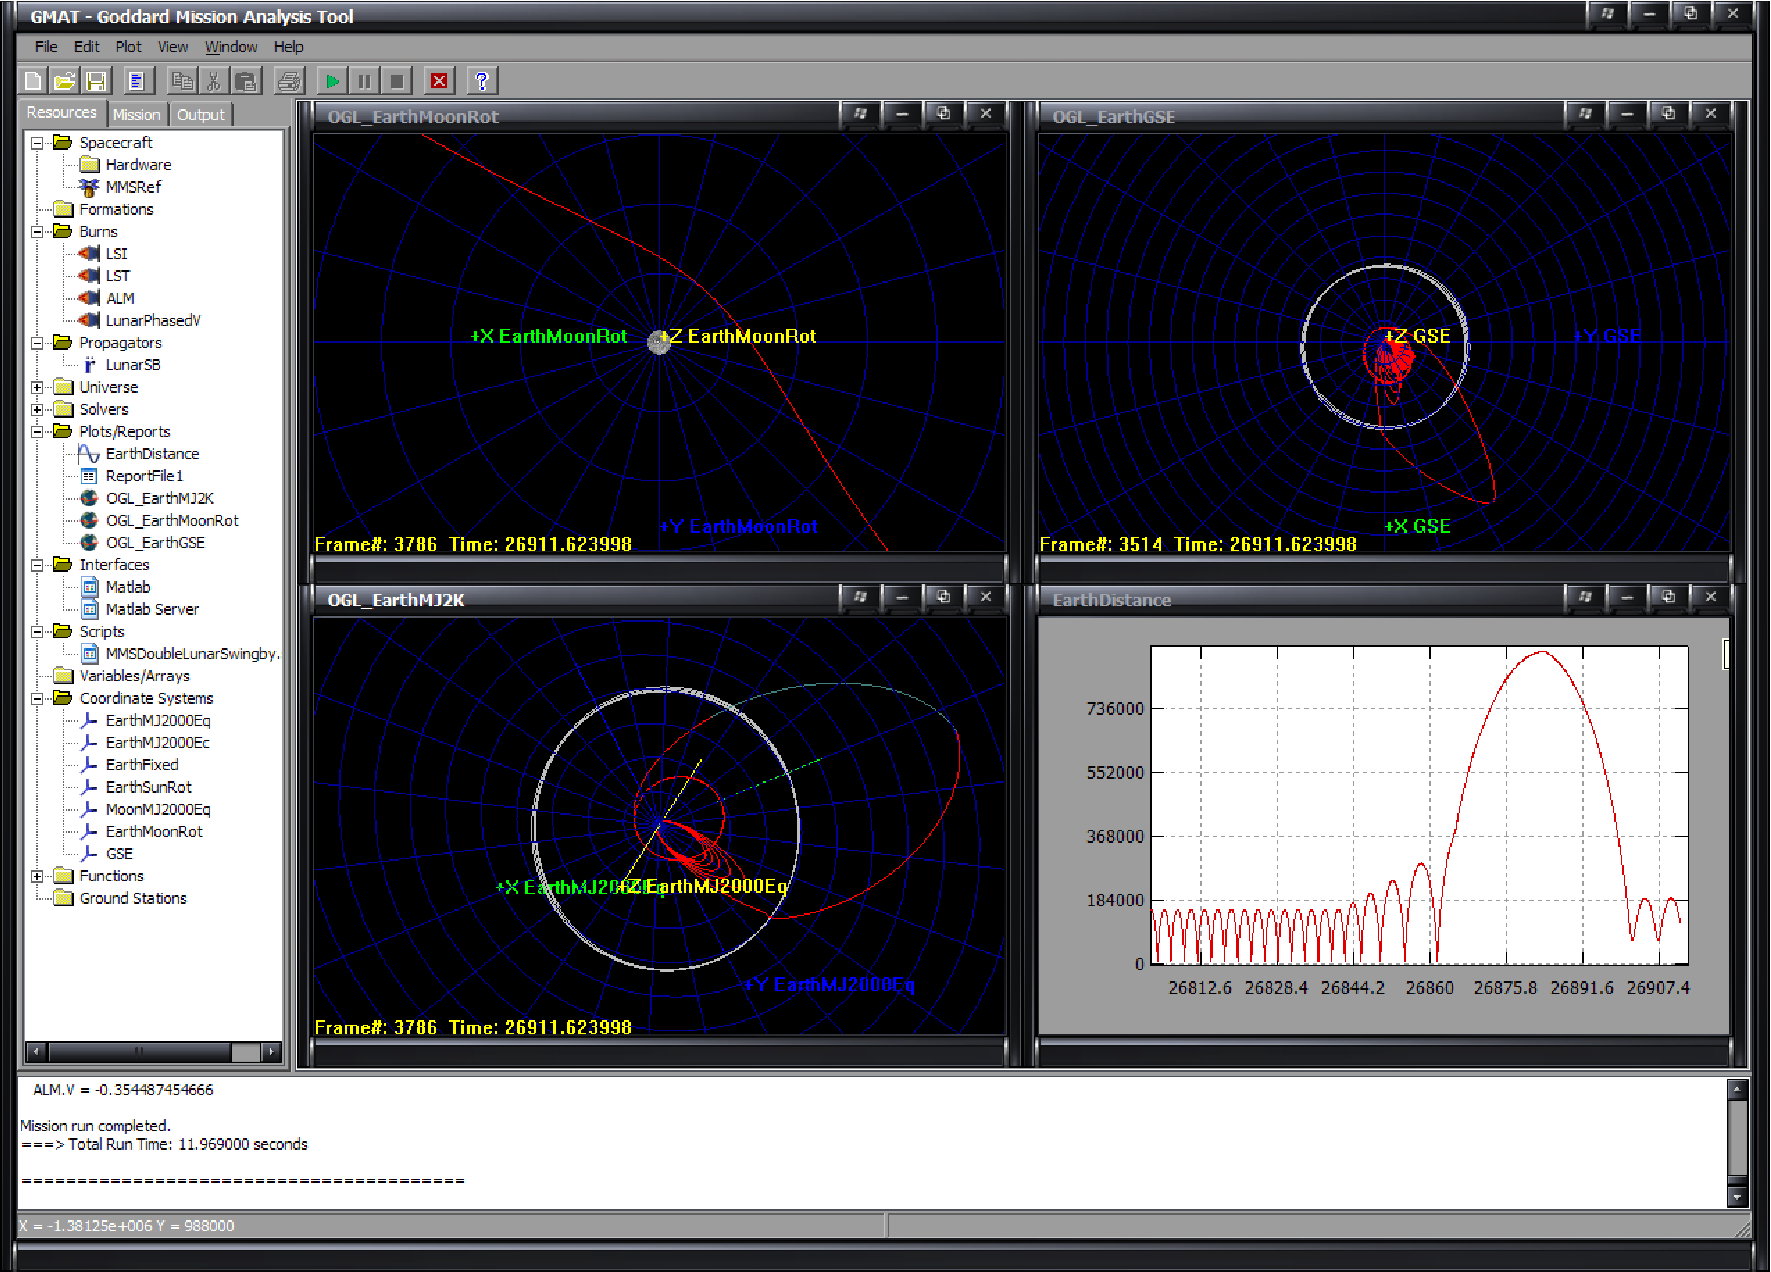
\includegraphics[width=\textwidth]{Images/DoubleLunarSwingby.png}
  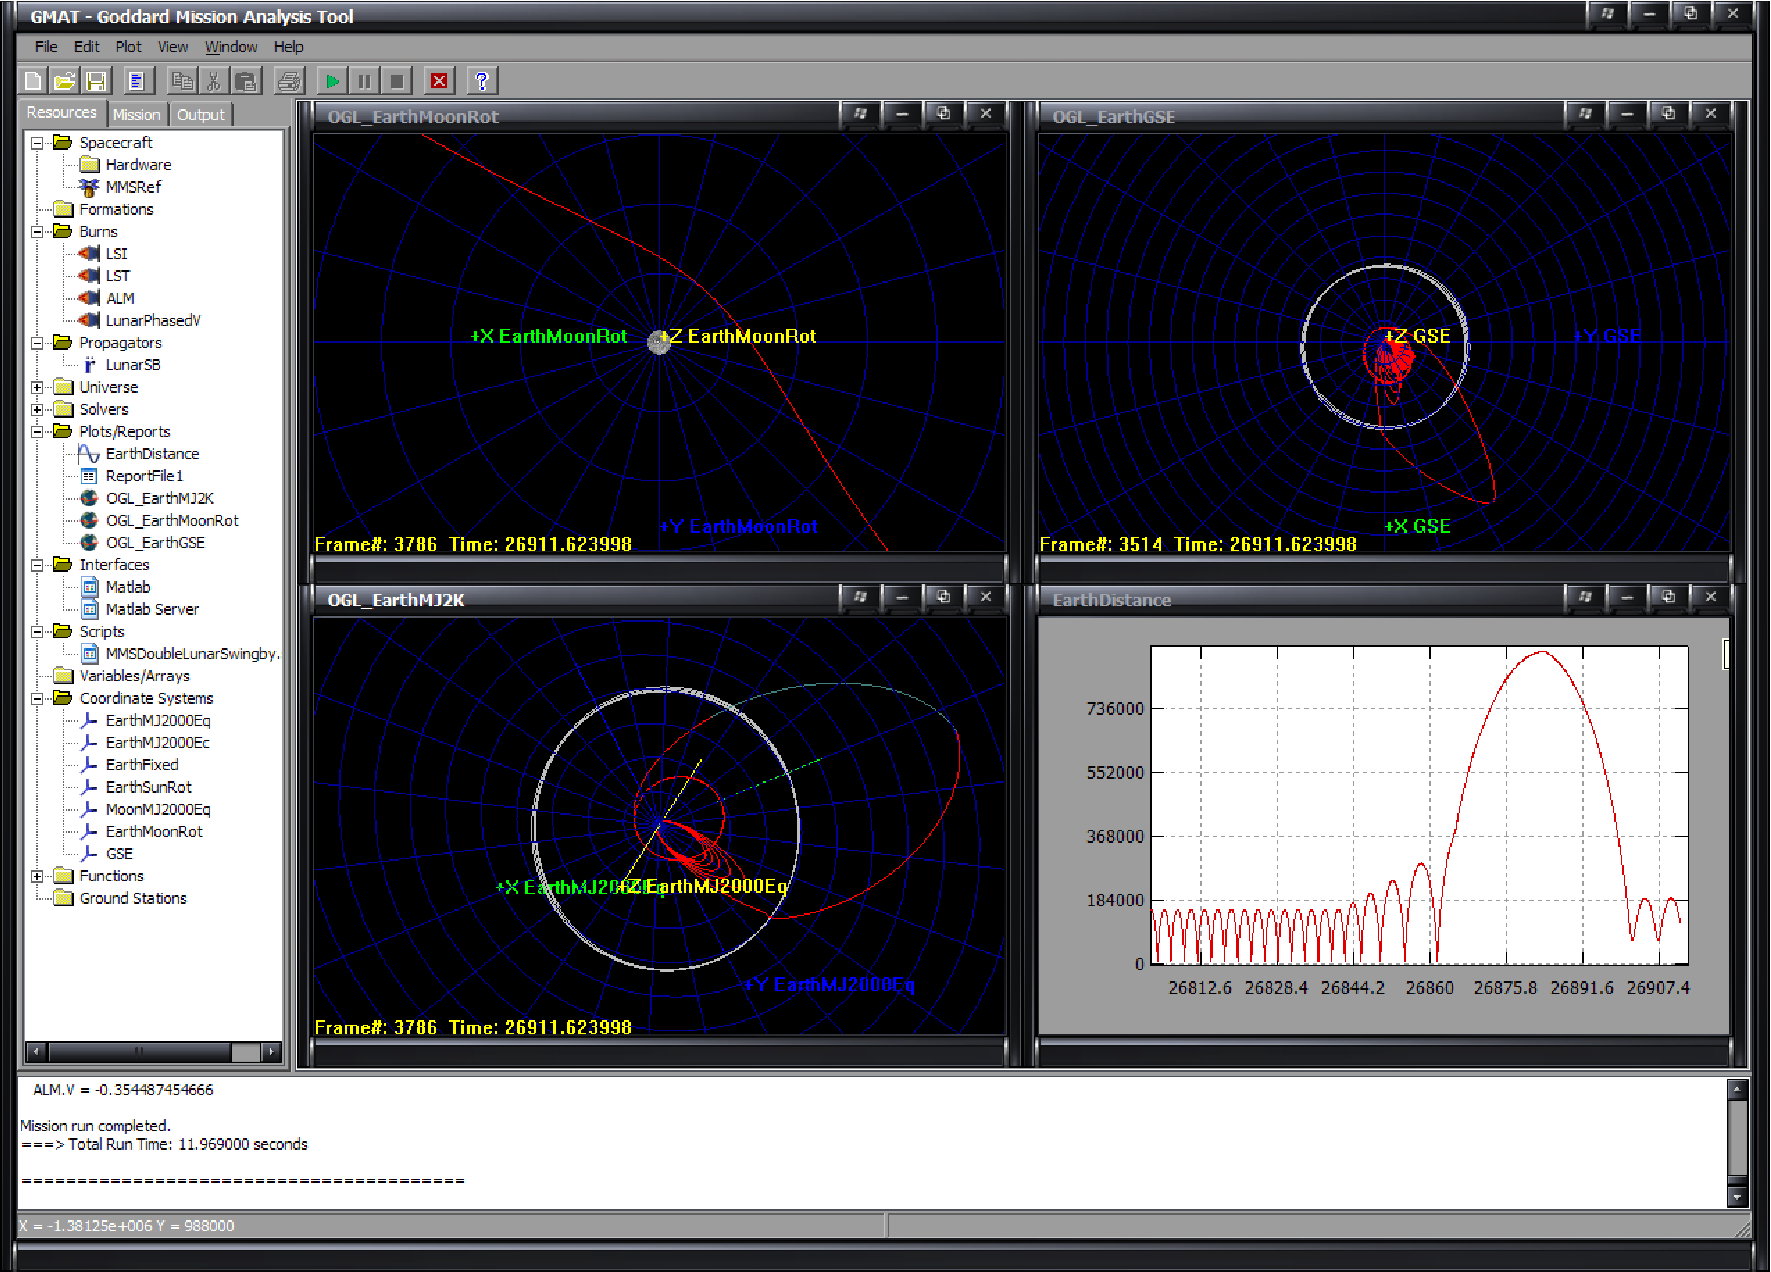
\includegraphics[scale=0.25]{Images/DoubleLunarSwingby.eps}
  \caption{A Sample GMAT Run}\label{DLS_Sample}
\end{center}
\end{figure}

\section{Design Criteria}

There are several high level requirements for GMAT that drove the design of the system.  These
requirements can be summarized in five broad categories: MATLAB Accessibility, Extensibility,
Formation Modeling, Parallel Processing, and Open Source Availability.  The system is designed to
run on Macintosh, Windows, and variants of Unix (including Linux) -- through a recompilation of the
source.

\subsection{MATLAB Accessibility}

MATLAB is a tool used at many facilities in the aerospace community to develop new algorithms and to
prototype approaches unique to new missions under consideration.  MATLAB as a system is quite
flexible, but is rather slow for precision orbit modeling work.  GMAT, by design, performs detailed
orbit and attitude modeling, providing an engine that can be called from MATLAB for tasks that
present performance issues when built in the MATLAB language.

\subsection{User Extensibility}

One prime driver for the development of GMAT was to provide a tool that allows users to try
new components and models in the system without rebuilding it from scratch.  This capability is
partially satisfied by the MATLAB interface described above.  Components of GMAT can also be added
to the system by writing new code that can be compiled into shared libraries and incorporated into
the system at run time.  All of the operating systems GMAT supports provide native methods for this
capability, and the system is designed to make the addition of new components simple using these
capabilities.

\subsection{Formation Modeling}

The current tool set used to model formations treats a formation of spacecraft as individual
spacecraft, modeled independently and then compared by matching states at specific epochs, either
on a small scale (taking single steps for each and then comparing the states) or on a large scale
(propagating ephemerides for each spacecraft and then going back afterwards to compare states at
specific epochs.  GMAT provides the ability to treat a collection of spacecraft as a single entity,
making the modeling more streamlined and providing the ability to handle formations and
constellations as simple entities.

\subsection{Parallel Processing Capabilities}

Some satellite analysis tasks require the execution of many separate orbit propagations, including
mission tuning (aka targeting or optimizing) and other mission refinements, in order to adequately
model the mission scenarios under analysis.  These tasks can take as many as several hundred
separate runs, each consisting of several minutes or more of run time on current hardware, in order
to determine the results of the analysis problem.  GMAT is designed to enable the parallelization of
these tasks across multiple processors, either within the same computer or, eventually, across a
network of computers.  While the current implementation does not leverage this capability, it is
designed to make the transition to multiple processors and distributed computing as simple as
possible.

\subsection{Open Source Availability}

GMAT is available for external users in both executable and source code form, subject to the NASA
Open Source licensing agreement.  This redistribution requirement drove design issues related to
the selection of external libraries and packages used by GMAT.

\section{Design Approach}

The categories described above drove the architecture of GMAT.  The following paragraphs describe
the architectural elements used to address these requirements.

\subsection{Modularity}

GMAT is a complicated system.  It is designed to be implemented using a ``divide and conquer''
approach that uses simple components that combine to satisfy the needs of the system.  This system
modularity makes the individual components simple, and also simplifies the addition of new
components into the system.  In addition, each type of resource has a well defined set of
interfaces, implemented through C++ base classes.  New components in each category are created by
implementation of classes derived from these base classes, building core methods to implement the
new functionality -- for example, forces used in the force model for a spacecraft all support an
interface, GetDerivatives(), that provides the acceleration data needed to model the force.  Users
can add new components by implementing the desired behavior in these interfaces and then registering
these components in the GMAT factory subsystem.

\subsection{Loose Coupling}

The modularity of the components in GMAT are implemented to facilitate ``plug and play'' capability
for the components that allows them to be combined easily using a set of common interfaces.
Components built in the system have simple interfaces to be able to communicate with MATLAB and with
one another.  Dependencies between the components are minimized.  Circular dependencies between
components minimized.

\subsection{Late Binding}

GMAT is designed to support running of multiple instances of a mission simultaneously in order to
satisfy parallel processing requirements.  This capability is built into the system by separating
the configuration of the components used in the mission from the objects used during execution.
Configured objects are copied into the running area (the ``Sandbox'') and then connected together to
execute the mission.  The connections between the components cannot be made until the objects are
placed in the Sandbox because the objects in the Sandbox are clones of the configured objects.  This
late binding makes parallelization simple to implement when the system is ready for it --
parallelization can be accomplished by running multiple Sandboxes simultaneously.

\subsection{Generic Access}

GMAT components share a common base class that enforces a set of access methods that are used to
serialize the components, facilitating both file level read and write access to the components and
simplifying communications with MATLAB and other external tools.  This capability is implemented
using parameter access methods that are themselves serialized, providing descriptors for each
parameter.  Connections between components are specified at this level by establishing parameters
that identify the connected pieces by name.  Data generated by the system is passed out of the
Sandbox through a message interface, using ``publish and subscribe'' design.

\section{Document Structure and Notations}

GMAT is written in ANSI C++.  The system is object-oriented, makes extensive use of the standard
template library (STL), and is coded based on a style guide\cite{shoan} so that the code conforms to
a consistent set of conventions.  The source is configuration managed in a CVS repository hosted at
GSFC.

This document provides a fairly in-depth introduction to the design of the software.  Throughout
this document, the architecture of the system is described using C++ nomenclature.  The design of
the system is illustrated using Unified Modeling Language (UML) diagrams to sketch the relationships
and program flow elements.  While this document is extensive, it does not completely document all
of the intricacies of each GMAT class.  These details can be found most accurately in the source
code, which is available on request under the NASA Open Source licensing agreement.  The code
includes comments written in a style compatible with the Doxygen documentation system.  When the
source code is processed by Doxygen, the output is a complete reference to the GMAT Application
Programmer's Interface (API).


\chapter{The GMAT Design Approach}

\section{Approach to Meeting Requirements}

\section{GMAT's Design Philosophy}

\section{Extendability Considerations}

\section{Platform Considerations}


% $Id: TopLevel.tex,v 1.1 2008/01/31 18:04:17 dconway Exp $
\chapter{\label{chapter:TopLevel}System Architecture Overview}
\chapauthor{Darrel J. Conway}{Thinking Systems, Inc.}

The purpose of this chapter is to introduce the key architectural elements of GMAT, and to explain
at a high level how they interact to solve mission design problems.  If you are trying to understand
how GMAT works, or if you are refreshing yourself in the basics of the GMAT architecture, this
chapter is where you should start.  After reading this chapter, you should have a high level
understanding of how the components in GMAT interact to perform mission analysis.

The chapter is written so that as you read further, you will obtain a deeper the view into the
system architecture.  We begin by identifying the key system components and grouping them according
to the functions they perform.  These groupings are referred to as ``Packages'' and are used to
provide a framework for the discussion about how GMAT works.

After presenting the functional GMAT's components, we present a high level view of how these
components interact and describe which components interact with each other.  This description
provides an overview of how messages and data flow in the system.  The next level of detail
describes how the architecture handles a simple application there a user open the system, creates a
spacecraft, configures a mission sequence, and runs the mission.

Later chapters build on these materials.  The remainder of this document is organized to take the
package descriptions presented at the start of this chapter, and present the design of the elements
of these packages.  Since the document is structured that way, we'll begin this chapter by examining
the logical packaging of GMAT's components.

\section{\label{section:Packaging}The GMAT System Framework}\index{Packages}

\begin{figure}
\begin{center}
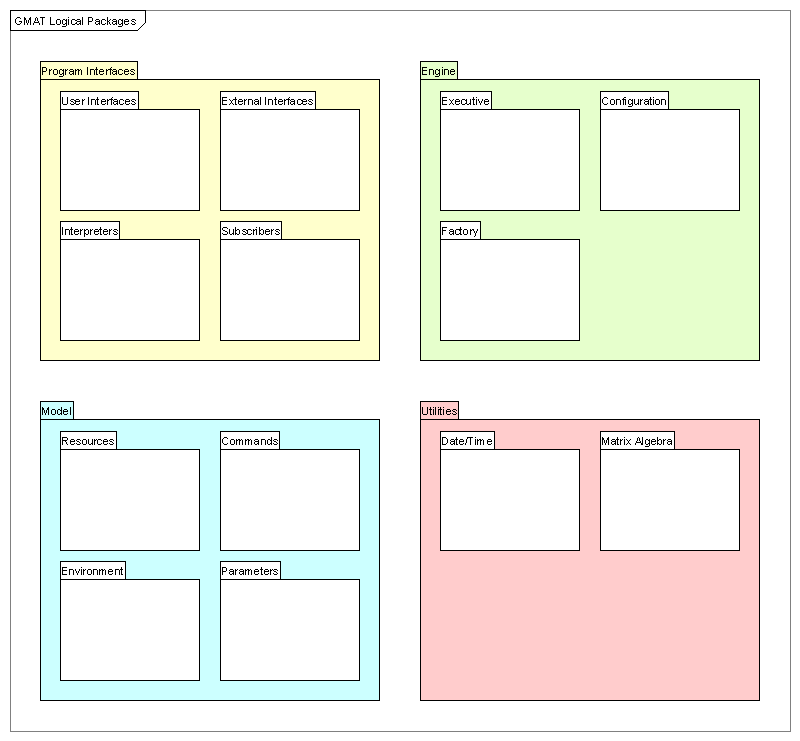
\includegraphics[400,371]{Images/GMATLogicalPackages.png}
\caption{\label{figure:TopLevelPackages}Top Level GMAT Packages: Logical Grouping}
\end{center}
\end{figure}

% Here is the packaging color scheme used throughout this chapter:
%    Interface package:  pale yellow    RGB: 255 255 153
%    Engine package:     pale green     RGB: 204 255 204
%    Model package:      pale cyan      RGB: 204 255 255
%    Utility package:    pink           RGB: 255 204 204
%    External programs:  pale orange    RGB: 255 204 153
%    GMAT Background:    light grey     RGB: 204 204 204

The GMAT architecture can be described as a set of components grouped into functional
packages\footnote{Note that these divisions are functional, and not enforced by any physical
packaging constraints like a namespace or shared library boundaries.} that interact to model
spacecraft missions.  The system is built around four packages that cooperatively interact to
model spacecraft in orbit. Figure~\ref{figure:TopLevelPackages} shows an overview of this package
grouping.  GMAT functionality can be broken into Program Interfaces, the core system Engine, the
Model used to simulate spacecraft and their environment, and Utilities providing core programmatic
functionality. The constituents of these packages are described throughout this document; this
chapter provides a framework for the more detailed discussions that follow.

Each of these functional categories can be broken into smaller units.  The next level of
decomposition is also shown in Figure~\ref{figure:TopLevelPackages}.  This next level of packaging
-- referred to as ``subpackaging'' in this document -- provides a finer grained view of the
functions provided in each package.  The next level of decomposition below the subpackages
provides a view into the class structure of GMAT, as will be seen in the next few paragraphs.

\subsection{Package and Subpackage Descriptions}

Figure~\ref{figure:PackageHierarchy} presents the packages and subpackages in a slightly different
format from that shown in the last figure.  The top level packages are represented by specific
colors matching those in Figure~\ref{figure:TopLevelPackages}\footnote{This color scheme will be
used for the remainder of this chapter as well.}.  The package names are listed at the top of each
column, with the subpackages shown indented one level from these packages.  One additional level is
shown in this diagram, showing representative members of the subpackages.  The deepest level items
in this figure are classes contained in the subpackages; for example, the Executive subpackage in
the Engine package contains the Moderator, Sandbox, and Publisher classes.  These elements will be
used in the discussion of how the packages interact in the next few pages of this document.

As is shown in these figures, three of these packages can be further broken into subpackages.  The
following paragraphs present an overview of the packages and their subdivisions.

\begin{figure}
\begin{center}
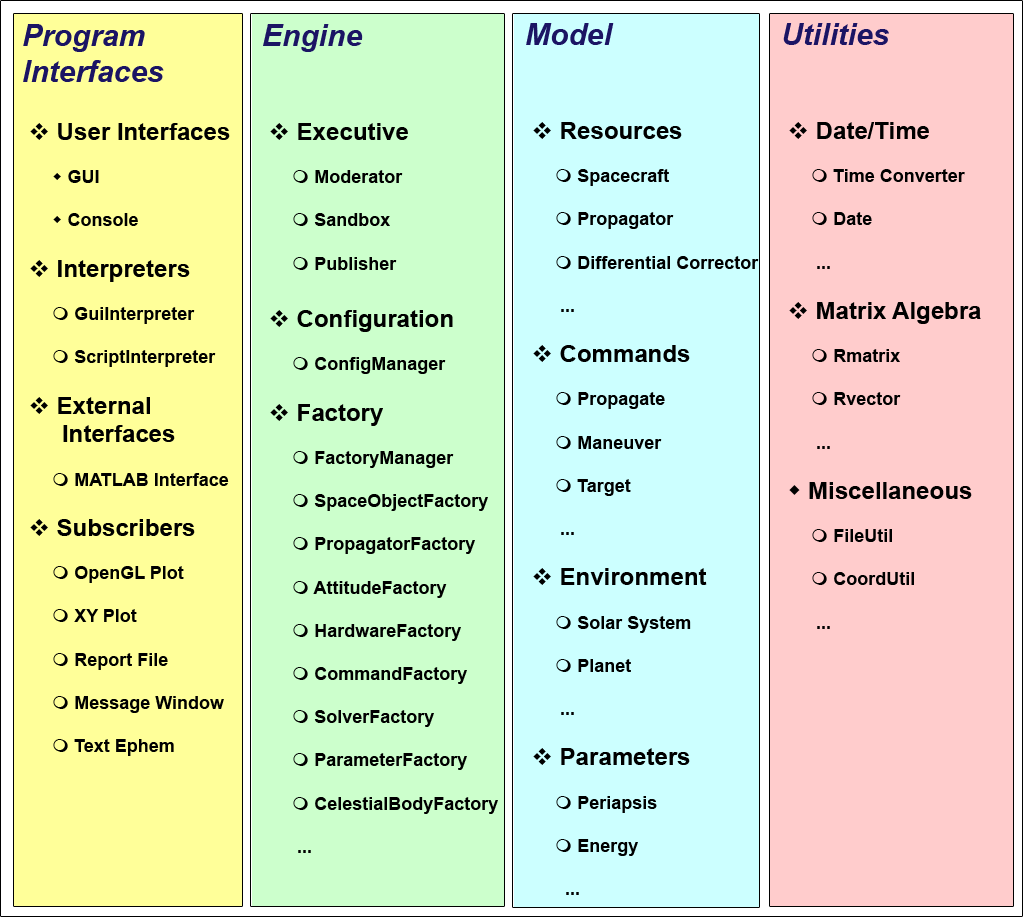
\includegraphics[445,399]{Images/PackageHierarchy.png}
\captionsetup{format=hang,justification=centerfirst,margin=96pt}
\caption[Packages, Subpackages, and Some Details]
{\label{figure:PackageHierarchy}Packages, Subpackages, and Some Details

Subpackages are indicated by a cluster of diamonds

Objects and Classes are marked by a circle

Other constructs are marked by a single diamond
}
\end{center}
\end{figure}

\begin{description}
\item[Program Interfaces] \index{Interfaces}All two-way communications between users and external
programs and GMAT are contained in the Program Interface package.  This package can be broken into
four subpackages:
  \begin{itemize}
    \item \textit{User Interfaces} \index{Interfaces!Program Interfaces}Users view GMAT through a
user interface -- usually through the GMAT Graphical User Interface (GUI), but also potentially
through a command line interface into GMAT called the GMAT console application, or Console.  These
interfaces are contained in the UserInterface subpackage.

    GMAT's GUI is coded using the wxWidgets cross-platform library\cite{wxWidgets}. The GUI provides
a rich environment that provides access to all of the features of GMAT through either panels
customized for each component or through a text based script.  Missions saved from the GUI are saved
in the script format, and scripts loaded into the GUI populate the GUI elements so that they can be
viewed on the customized interface panels.

    The console version of GMAT can be used to run script files and generate text data with little
user interaction.  The console application can run multiple scripts at once, or individual scripts
one at a time.  This version of the system is currently used for testing purposes, in situations
where the overhead of the full graphical user interface is not needed.

    \item \textit{Interpreters}\index{Interpreters!Overview} The user interface components
communicate with the core GMAT system through an interface layer known as the Interpreter
subpackage.  This layer acts as the connection point for both the scripting interface and the GUI
into GMAT.

    The Interpreter subpackage contains two specific interpreters: a GuiInterpreter, designed to
package messages between the GUI and the GMAT engine, and the ScriptInterpreter, designed to parse
script files into messages for the engine, and to serialize components in the engine into script
form for the purposes of saving these objects to file.

    The Interpreter subpackage is designed so that it can be extended to provide other means of
controlling the GMAT engine.  All that is required for this extension is the development of a new
interpreter, and interfaces for this new component into the Moderator, a component of the Executive
subpackage in GMAT's Engine package.

    \item \textit{External Interfaces} \index{Interfaces!External Interfaces}GMAT provides an
interface that can be used to communicate with external programs\footnote{At this writing, the only
external interface incorporated into the core GMAT code base is an interface to the MathWorks'
product MATLAB\cite{MATLAB}.}.  These interfaces are packaged in the ExternalInterfaces subpackage.

    \item \textit{Subscribers} \index{Interfaces!Subscribers}\index{Subscribers}Users view the
results of a mission run in GMAT through elements of the Subscriber subpackage.  Subscribers are
used to generate views of spacecraft trajectories, plots of mission parameters, and reports of
mission data in file form.

  \end{itemize}
  \item[The Engine] \index{Engine}The interfaces described above exist on top of a core simulation
engine used to control the model of flight dynamics problems in GMAT.  This engine consists of the
control and management structures for the program. The elements of the model used to simulate the
spacecraft mission are introduced in the next package description.  The Engine package consists of
three subpackages:
  \begin{itemize}
    \item \textit{Executive} \index{Engine!Executive Components}The Executive subpackage contains
the central processing component for GMAT (called the Moderator), a connection point used to capture
and distribute the results of a mission run (the Publisher), and the workspace used to run a mission
(the Sandbox).

    The Moderator acts as the central communications hub for the GMAT engine.  It receives messages
from the program interfaces through the interpreters, and determines the actions that need to be
taken based on these messages.  The Moderator sends messages to the other components of the Engine
to accomplish the requested tasks.

    GMAT is designed to run missions inside of a component called the Sandbox.  When a user requests
a mission run, the Moderator sets up the Sandbox with the elements configured for the run, and then
turns control over to the Sandbox to execute the mission.

    The Publisher acts as the connection between data generated in the Sandbox and the views of
these data presented to the User.  It receives data or instructional messages from the components in
the Sandbox, and passes those messages to the corresponding Subscribers.

    \item \textit{Configuration} \index{Engine!The Configuration}When GMAT builds a model, it starts
by building components that will be connected together based on a sequence of instructions.  Each
component is an instance of a GMAT class; as they are built, these components are stored in a local
repository of objects. The repository holding model components is known as the configuration.  The
Configuration subpackage consists of this repository and an interface used to access it, called the
ConfigurationManager.

    The components stored in the configuration are all derived from a base class named GmatBase,
described in Chapter~\ref{chapter:CoreClasses}.  In GMAT, every object that a user creates and uses
to simulate a spacecraft mission is derived from this base class.  The configuration is maintained
as a collection of pointers to GmatBase objects.  The ConfigurationManager works with this
collection to maintain the configuration repository.

    \item \textit{Factory} \index{Engine!Factories}\index{Factory!Overview}The model elements stored
in the configuration are created on request from the users.  The subpackage responsible for
processing requests for new model elements is the Factory subpackage.  It consists of an interface
into the subpackage -- the FactoryManager -- and a collection of factory classes used to create
specific types of model elements.

    Each factory in GMAT creates objects based on the type requested.  For example, Spacecraft or
Formation objects are created through a call is the corresponding type of object into the
SpaceObjectFactory.  Similarly, if a user needs a Prince-Dormand 7(8) integrator, a call is made to
the PropagatorFactory for that type of integrator.  The factory creates the object through a call to
the class's constructor, and returns the resulting object pointer.

    The Factory subpackage is constructed this way to facilitate extensibility.  Users can add user
generated classes by creating these classes and a Factory to instantiate them.  That factory can
then be registered with GMAT's FactoryManager, and users will be able to access their specialized
classes in GMAT without modifying the configured GMAT code base.  Eventually, users will be able to
load their objects through shared libraries (aka dlls in the Windows world) at run time.

    The FactoryManager registration process takes a factory and asks it what type of objects it can
create, and sends the corresponding requests to the correct factory.  Details of the factories
themselves can be found in Chapter~\ref{chapter:Factories}.  Extensibility is discussed in
Chapter~\ref{chapter:ExtendingGMAT}.
  \end{itemize}
  \item[The Model] \index{Model}The Engine package, described above, provides the programmatic
framework necessary for building and running a simulation in GMAT.  The objects that are used to
model the elements of the simulation are contained in the Model package.  All of the elements of the
Model package are derived from a common base class, GmatBase, described in
Chapter~\ref{chapter:CoreClasses}.

  When a user configures GMAT to simulate a spacecraft mission, the user is configuring objects in
the Model package.  In other words, the Model package contains all of the components that are
available to a user when setting up a mission in GMAT.  The model elements can be broken into four
subpackages:

  \begin{itemize}
    \item \textit{Environment} \index{Model!Environment}The environment subpackage provides all of
the background environmental data used in GMAT to model the solar system, along with the components
needed to perform conversions that require these elements.
    \item \textit{Resources} \index{Model!Resources}All of the model elements that do not require
some form of sequential ordering in GMAT are called Resources.  These are the model elements that
appear in the Resource tree in the GUI -- excluding the Solar System elements -- and they are the
elements that are stored in the configuration subpackage, described above.
    \item \textit{Commands} \index{Model!Commands}Commands are the elements of the model that
describe how the model should evolve over time.  Since commands are sequential, they are stored
separately, and in sequential order, in the Command subpackage.  The sequential set of commands in
GMAT is called the Mission Control Sequence.

    The Mission Control Sequence is a list of commands.  Commands that allow branching manage their
branches through ``child'' lists.  These branch commands can be nested as deep as is required to
meet the needs of the model.
    \item \textit{Parameters} \index{Model!Parameters}Parameters are values or data containers (e.g.
variables or arrays) that exist external to other objects in the GMAT model.  These objects are used
to perform calculations of data useful for analysis purposes.
  \end{itemize}
  \item[Utilities] \index{Utilities}The Utility package contains classes that are useful for
implementing higher level GMAT functions.  These core classes provide basic array computations, core
solar system independent calculations, and other useful low level computations that facilitate
programming in the GMAT system.
\end{description}

\subsection{Package Component Interactions}

The preceding section provides a static view into the components of GMAT.  In this section, a
high level view of the interactions between the elements of these packages will be described.
Figure~\ref{figure:TopLevelPackages} shows the static package view of GMAT.  Each top level package
is color coded so that the system components shown in the interaction diagram,
Figure~\ref{figure:GMATStackDiagram}, can be identified with their containing package.  The legend
on this figure identifies the package color scheme.

\begin{figure}
\begin{center}
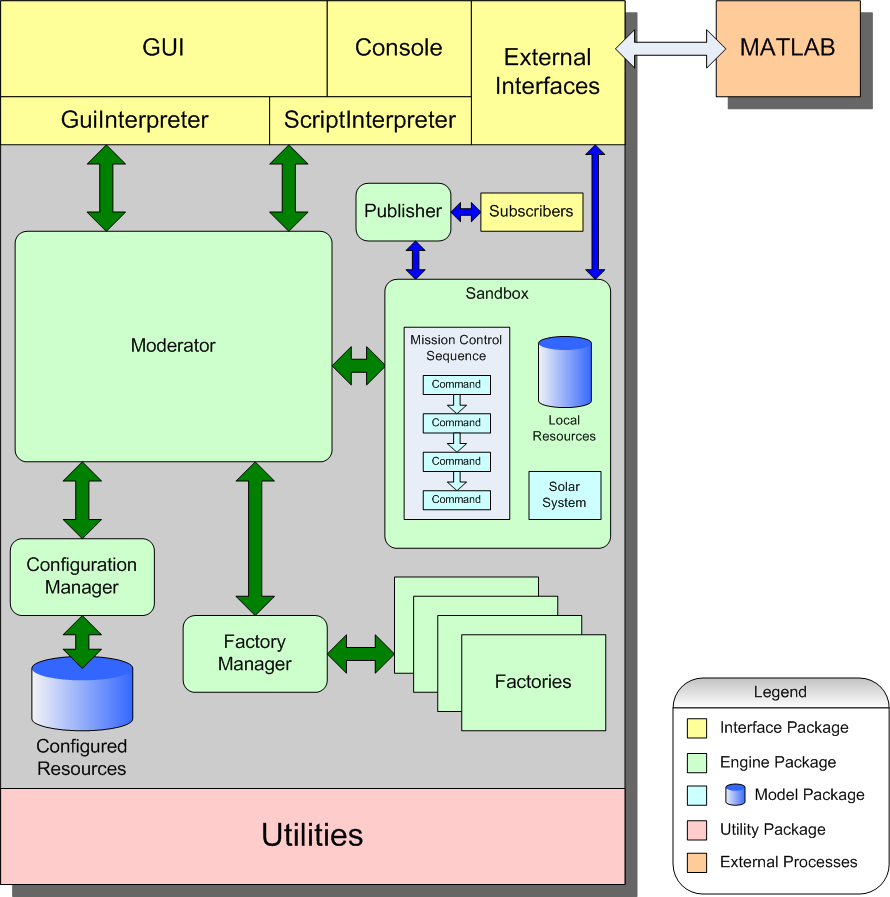
\includegraphics[445,449]{Images/GMAT_Stack.png}
\caption[Subsystem Interactions in GMAT]{\label{figure:GMATStackDiagram}Subsystem Interactions in
GMAT\\Green arrows show information flow between the core Engine components, while blue arrows show
information flow that occurs when a mission is executed.}
\end{center}
\end{figure}

Users interact with GMAT through either a Graphical User Interface (GUI) written using the
cross-platform GUI library wxWidgets, or through a console-based application designed to
run scripts without displaying graphical output.  These interfaces communicate with the GMAT engine
through interpreter singletons\footnote{\index{Singleton}\index{Design Patterns!Singleton}The GMAT
engine is run through a set of singleton class instances.  The singleton design pattern used for
these instances is introduced in Appendix~\ref{chapter:Patterns}.  The important thing to know about
singletons for this discussion is that there is only one instance of any singleton class; hence a
running GMAT executable has one and only one ScriptInterpreter, and Moderator, and at most one
GUIInterpreter.  Other singletons will be introduced during this discussion as well, when the
factories and configuration are discussed.}.  The GUI application interacts with the engine through
both the Script and GUI Interpreters, while the console application interacts through the script
interpreter exclusively.  These interpreters are designed to mediate two-way communications between
the GMAT engine and users.   The GUI and console applications drive the GMAT engine through these
interpreters.

The Interpreters in turn communicate with GMAT's Moderator singleton.  The Moderator is the central
control object in the GMAT engine.  It manages all program level communications and information flow
while the program is running.  It receives messages from the interpreters, processes those messages,
and instructs other components of the engine to take actions in response to the messages.  The
messages sent by the interpreters fall into several distinct groups:

\begin{itemize}
\item\textbf{Object Creation} messages are used to request the creation of resources stored in the
configuration database or the creation of commands stored in the Mission Control Sequence.
\item\textbf{Object Retrieval} messages are used to access created objects, so they can be modified
by users or stored to file.
\item\textbf{Run} messages prepare the Sandbox for a run of the Mission Control Sequence, and then
launch execution of the Mission Control Sequence.
\item\textbf{Polling} messages are used to control an executing Mission Control Sequence, and are
used to coordinate external communications (for example, the startup process for MATLAB) and user
actions taken during the run.
%\item\textbf{Reset} messages are used to clear the configuration database and Mission Control
% Sequence so that a new model can be built in the engine.
\end{itemize}

\noindent The message and information flow in the Engine are shown in
Figure~\ref{figure:GMATStackDiagram} with double headed arrows.  The green arrows show the central
message and information flow in the engine, while the blue arrows show information flow that occurs
while a mission control sequence is executing.  These messages are described briefly here, and more
completely through examples later in this chapter.

The Moderator responds to requests for new resources or commands by requesting a new object from the
FactoryManager.  The FactoryManager determines which Factory class can supply the requested object,
and sends a ``create'' request to that factory.  The Factory builds the requested object, and sends
the pointer to the new object to the FactoryManager, which in turn sends the pointer to the
Moderator.  The Moderator sends the new object's pointer to one of two locations, depending on the
type of object created.  If the object is a Resource, the object pointer is passed to the
ConfigurationManager.  The ConfigurationManager adds the resource to the database of configured
objects.  If the requested object is a command, it is added to the Mission Control Sequence.  The
Moderator then returns the pointer to the interpreter that requested the new object.

Object retrieval is used to retrieve the pointer to an object that was previously created.  The
Moderator receives the message asking for the object.  If the object is a configured resource, it
calls the ConfigurationManager and asks for the resource by name.  Otherwise, it traverses the
Mission Control Sequence until it finds the requested command, and returns the pointer to that
command.

% Trying to fix a small nit with figure placement here
\begin{figure}
\begin{center}
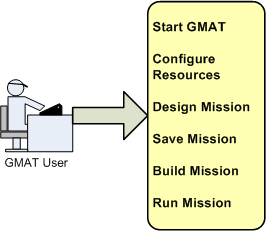
\includegraphics[133,116]{Images/GMAT_UserPerspective.png}
\caption{\label{figure:UserWorkFlow}User Interactions}
\end{center}
\end{figure}

Run messages are used to transfer the resources and Mission Control Sequence into the Sandbox and
start a run of the mission.  When the Moderator is instructed to run a Mission Control Sequence, it
starts by loading the configured components into the Sandbox.  The Moderator requests objects from
the ConfigurationManager, by type, and passes those objects to the Sandbox.  The Sandbox receives
the object pointers, and clones each object into a local resource database.  These local clones are
the objects that interact with the commands in the Mission Control Sequence to run a mission.  The
Moderator then passes the Mission Control Sequence to the Sandbox so that the Sandbox has the list
of commands that need to be executed to run the mission.  Next Moderator tells the Sandbox to
initialize its components.  The Sandbox initializes each of the local components, and establishes
any necessary connections between components in response to this message.  Finally, the Moderator
instructs the Sandbox to execute the Mission Control Sequence.  The Sandbox starts with the first
command in the sequence, and runs the commands, in order, until the last command has executed or the
run is terminated by either a user generated interrupt or an error encountered during the run.

Polling messages are used to process messages between the Moderator and the Sandbox during a run.
Typical messages processed during polling are user requests to pause or terminate the run, or to
open a connection to an external process (including the startup of that process).

The descriptions provided here for these message types may be a bit confusing at first.  The
following section provides representative cases of the message passing and object interactions in
GMAT when a user performs several common interactions.

\section{\label{section:TopLevelUseCase}GMAT Workflow Overview}

When users run GMAT, they follow a work flow like that shown in Figure~\ref{figure:UserWorkFlow}.
Users start the program, configure resources, plan their mission, save the configuration, build the
mission if working from a script file, and run the mission.  The following sections describe the top
level actions taken by GMAT when a user initiates each of these actions.

\subsection{\label{section:GMATStartup}The GMAT Startup Process}\index{Startup}

\begin{figure}[htb]
\begin{center}
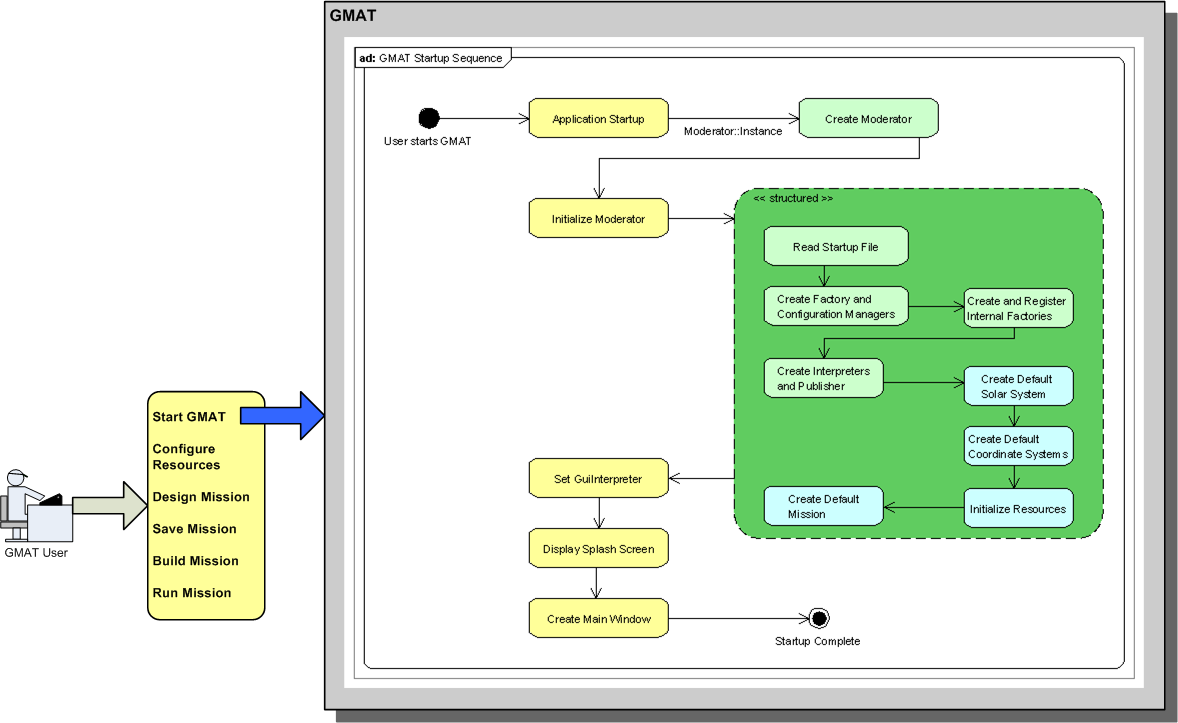
\includegraphics[450,277]{Images/GMAT_Startup.png}
\caption{\label{figure:StartupActivities}The Startup Process}
\end{center}
\end{figure}

The startup process for GMAT, shown in Figure~\ref{figure:StartupActivities}, launches the
executable program and prepares the engine for use.  Most of the work performed during startup is
performed by the Moderator.  When the application launches, the first action taken is the creation
of the Moderator singleton, made by calling the static Instance() method on the Moderator class.
This freshly created Moderator is then initialized by the application through a call to the
Initialize{} method.

The procedure followed in Initialize() is shown in the large green structured flow box in the
figure.  The Moderator reads the GMAT startup file, setting linkages to the default files needed to
model and display running missions.  The startup file resides in the same folder as the GMAT
application, and contains path and file information for planetary ephemerides, potential models,
graphical images used to provide texture maps for bodies displayed in the GUI, atmospheric model
files, and default output paths for log files and other GMAT generated outputs.

Upon successful read of the startup file, the Moderator starts creating and connecting the main
components of the engine.  It begins by creating the components used for building model elements.
The FactoryManager and ConfigurationManager are created first.  Next the Moderator creates each of
the internally configured factories, one at a time, and passes these instances into the
FactoryManager.  This process is called ``registering'' the Factories in other parts of this
document.  Upon completion of Factory registration, the Moderator creates instances of the
ScriptInterpreter and GuiInterpreter singletons and the Publisher singleton.  This completes the
configuration of the core engine elements, but does not complete the Moderator initialization
process, because GMAT starts with several default model elements.

The Moderator creates a default Solar System model, populated with a standard set of solar system
members.  Next it creates three default coordinate systems that always exist in GMAT configurations:
the Earth-Centered Mean of J2000 Earth Equator system, the Earth-Centered Mean of J2000 Ecliptic
system, and the Earth-Centered Earth body-fixed system.  Next the Moderator sets the pointers
needed to interconnect these default resources.  Finally, the Moderator creates a default mission,
and upon success, returns control to the GMAT application.

The Application retrieves the pointer for the GuiInterpreter, and sets this pointer for later use in
the GUI.  It then displays the GMAT splash screen, and then finally creates and displays the main
GMAT Window.  At this point, the GMAT GUI is configured and ready for use building models and
running missions.

\subsection{Configuring Resources}\index{Model!Resources}

\begin{figure}[htb]
\begin{center}
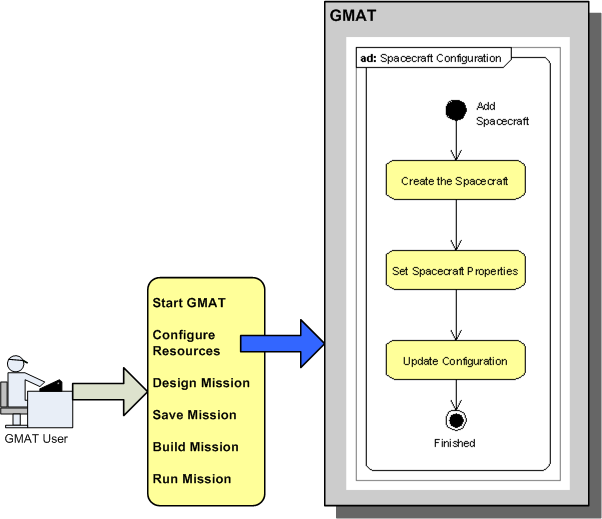
\includegraphics[301,260]{Images/GMAT_ConfigureResource.png}
\caption{\label{figure:ResourceConfig}Configuration Example: Spacecraft}
\end{center}
\end{figure}

Figure~\ref{figure:ResourceConfig} shows the top level set of actions taken by a user when
configuring a typical resource -- in this case, a Spacecraft object -- from the GUI.  The user
starts by using a right click on the Spacecraft folder (or control-click on the Mac) in the
resource tree on the left side of the main GMAT window.  This action opens a context menu; the user
selects ``Add Spacecraft'' from this menu, and a new spacecraft resource appears in the resource
tree.  This action is represented by the box labeled ``Create the Spacecraft'' in the figure.  The
user may also elect to change the name of the new Spacecraft.  This action is taken with a right
click (control-click on the Mac) on the new resource in the resource tree, and selecting
``Rename'' from the resulting context menu.

Once a resource has been created, the user can edit the properties of the resource.  From the GUI,
this action is performed with a double click on the resource.  The double click opens a new panel
tailored to the type of resource that is selected; for a Spacecraft, the panel shown in
Figure~\ref{figure:SpacecraftConfigPanel} opens.  The second block in
Figure~\ref{figure:ResourceConfig}, labeled ``Set Spacecraft Properties'', represents the actions
taken in GMAT when the user performs this selection, and when the user makes changes on the
resulting panel.

\begin{figure}[htb]
\begin{center}
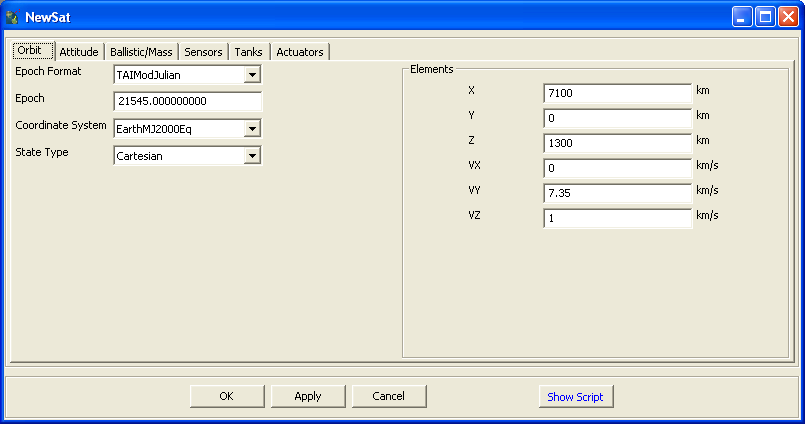
\includegraphics[403,212]{Images/SpacecraftPanel.png}
\caption{\label{figure:SpacecraftConfigPanel}The Spacecraft Configuration Panel}
\end{center}
\end{figure}

Changes made in a GUI panel like the one shown here are not automatically made on the underlying
objects in GMAT.  Changes made on the panel are fed back to the internal objects when the user
selects either the ``Ok'' or ``Apply'' button on the bottom of the panel.  This updating of the
resource is represented by the ``Update Configuration'' block in Figure~\ref{figure:ResourceConfig}.

Each of these blocks can be further decomposed into the internal actions performed in GMAT when the
user makes the selections described here.  The following paragraphs describe in some detail how GMAT
reacts to each of these user actions.

\subsubsection{\label{section:ObjectCreation}Creating the Spacecraft}

\begin{figure}[htb]
\begin{center}
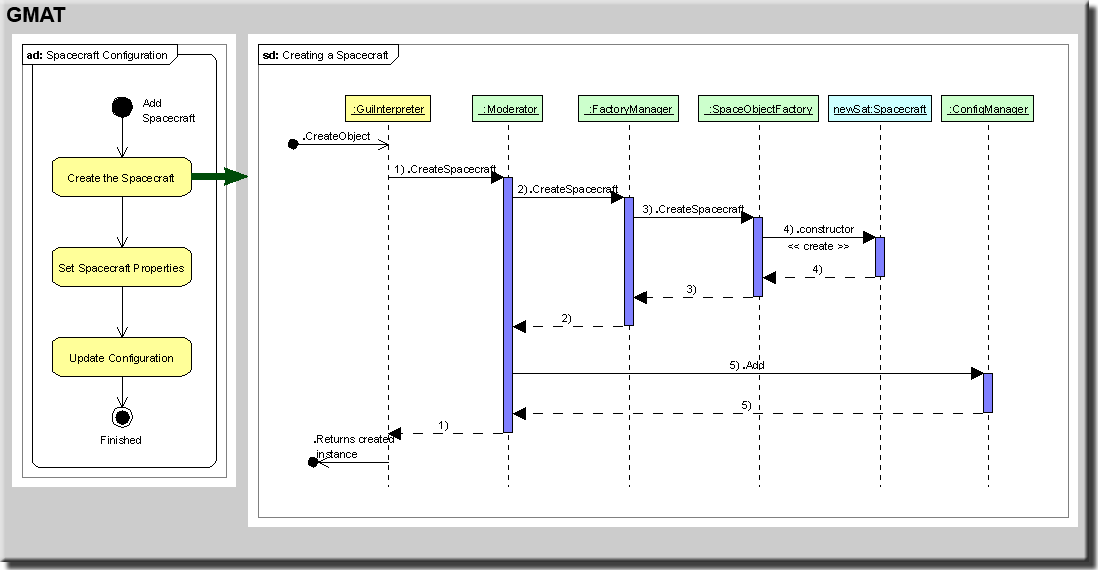
\includegraphics[460,239]{Images/SpacecraftCreation.png}
\caption[Configuration Example: Creating the
Spacecraft]{\label{figure:CreatingResource}Configuration Example: Creating the Spacecraft}
\end{center}
\end{figure}

Figure~\ref{figure:CreatingResource} shows an example of the process followed in GMAT when a new
resource is created from the GUI.  The user selected ``Add Spacecraft'' from the option menu on the
Spacecraft node of the resource tree (accessed with a right click -- control-click on the Mac -- on
the node).  This selection triggered the chain of events shown in the sequence diagram in the
figure\footnote{For an introduction to the UML diagram notation used throughout this document, see
Appendix~\ref{chapter:UMLDiagrams}}.  The sequence starts with a CreateObject() call from the GUI to
the interface into the GMAT engine.  The interface between the GUI and the GMAT engine is a
singleton instance\footnote{Singletons, and other design patterns used in GMAT, are introduced on
Appendix~\ref{chapter:Patterns}.} of the GuiInterpreter class, and is shown in green in the figure.

The GuiInterpreter singleton receives the call to create an object of type Spacecraft.  It makes a
call, in turn, into the singleton responsible for running the GMAT engine.  This singleton is an
instance of the Moderator class\footnote{For the purposes of this discussion, the singleton
instances will be referred to by their class name for the remainder of this discussion.}.  The call
into the Moderator is made in step 1 of the diagram; the call is made through the CreateSpacecraft()
method of the Moderator.

User configured objects in GMAT are always created through calls into a subsystem referred to
collectively as the Factory subsystem.  Factories are responsible for creating these objects.  The
factory subsystem is managed through a singleton class, the FactoryManager.  The Moderator accesses
the factories through this singleton.  In step 2 of the figure, the Moderator makes a call to the
CreateSpacecraft() method on the FactoryManager.  The FactoryManager finds the Factory responsible
for creating objects of the type requested -- in this case, a Spacecraft object -- and calls that
factory in turn.  Spacecraft are created in GMAT's SpaceObjectFactory, so the FactoryManager calls
the CreateSpacecraft() method on the SpaceObjectFactory, as is shown in step 3.

The SpaceObjectFactory creates an instance of the Spacecraft class by calling the class's
constructor, as shown in step 4.  The constructed object is given a name, and then returned
through the FactoryManager to the Moderator.  The Moderator receives the new object, and adds it to
the database of configured objects in GMAT.

All configured GMAT objects are managed by a singleton instance of the ConfigurationManager class.
The ConfigurationManager is used to store and retrieve objects during configuration of the model.
The Moderator adds created components to the configuration by calling Add() methods on the
ConfigurationManager.  For this example, the new Spacecraft is added to the configuration through
the call shown in step 5.

Once the steps described above have been completed successfully, the Moderator returns control to
the GuiInterpreter, which in turn informs the GUI that a new object, of type Spacecraft, has been
configured.  The GUI adds this object to the resource tree, and returns to an idle state, awaiting
new instructions from the user.

\subsubsection{\label{section:ObjectConfiguration}Setting Spacecraft Properties}

The Spacecraft that was created above has default settings for all of its properties.  Users will
typically reset these properties to match the needs of their mission.  The process followed for
making these changes from the GUI is shown in Figure~\ref{figure:ConfiguringResource}.

\begin{figure}[htb]
\begin{center}
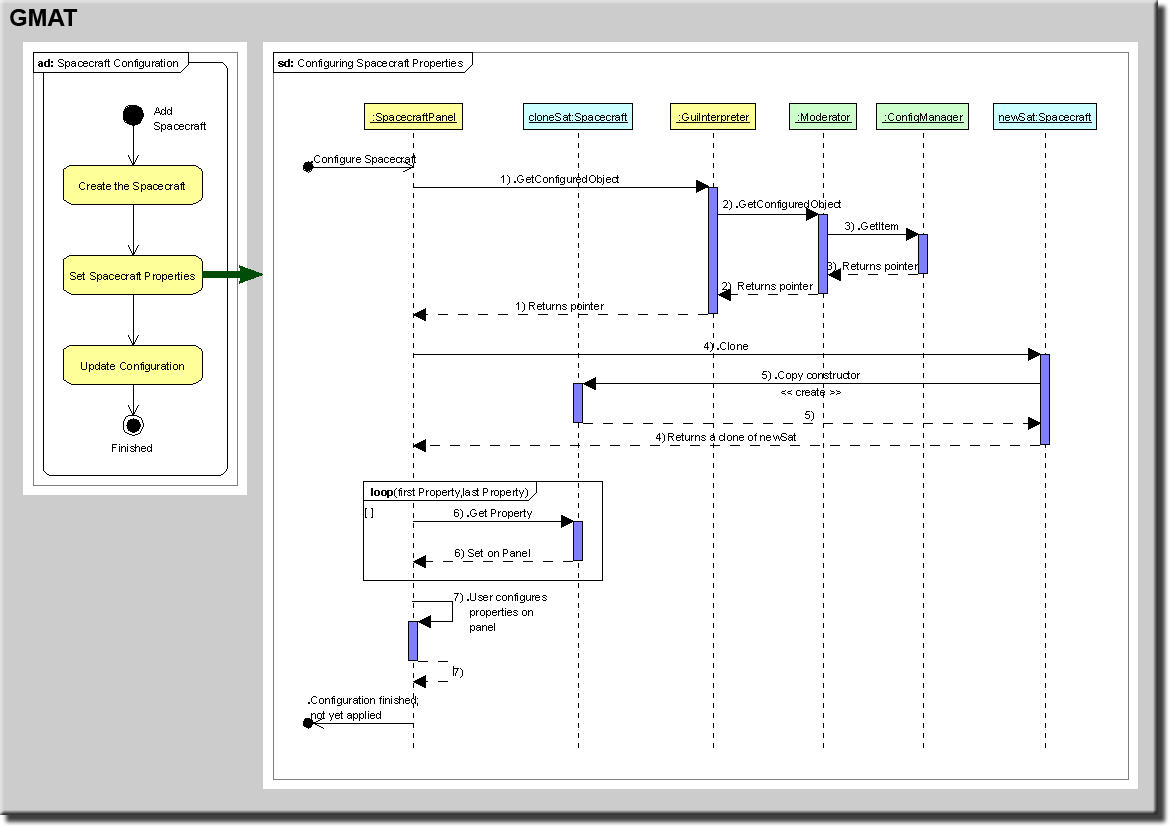
\includegraphics[460,326]{Images/SpacecraftConfiguration.png}
\caption{\label{figure:ConfiguringResource}Configuration Example: Setting Spacecraft Properties}
\end{center}
\end{figure}

As was discussed in the introduction to this section, Spacecraft properties are set on the GUI panel
shown in Figure~\ref{figure:SpacecraftConfigPanel}.  Users can open this panel at any point in the
model setup process.  Because of the free flow in the configuration process, the Spacecraft pointer
may not be accessible when the user elects to open the configuration panel with a double click on
the Spacecraft's name on GMAT's resource tree.  Therefore, the first action taken when the panel is
opened is a call from the panel to the GuiInterpreter to retrieve the configured Spacecraft with the
name as specified on the Resource tree.  The GuiInterpreter passes this request to the Moderator.
The Moderator, in turn, asks the ConfigurationManager for the object with the specified name.  The
ConfigurationManager returns that object to the Moderator, which passes it to the GuiInterpreter.
The GuiInterpreter returns the object (by pointer) to the Spacecraft Panel.

The Spacecraft Panel creates a temporary clone of the configured spacecraft so that it has an object
that can be used for intermediate property manipulations\footnote{The Spacecraft is unique in this
respect; other objects configured in the GMAT GUI are manipulated directly, rather than through a
clone.  The Spacecraft is in many respects a composite object; this added complexity makes the
intermediate clone a useful construct.}.  This clone is set on the Spacecraft Panel's subpanels,
accessed through a tabbed interface shown in the snapshot of the panel.  Each subpanel accesses the
properties corresponding to the fields on the subpanel, and sets its data accordingly. The
Spacecraft Panel is then displayed to the user.  The user then makes any changes wanted for the
model that is being configured.

\subsubsection{\label{section:ObjectPersistance}Saving the Spacecraft}

\begin{figure}[htb]
\begin{center}
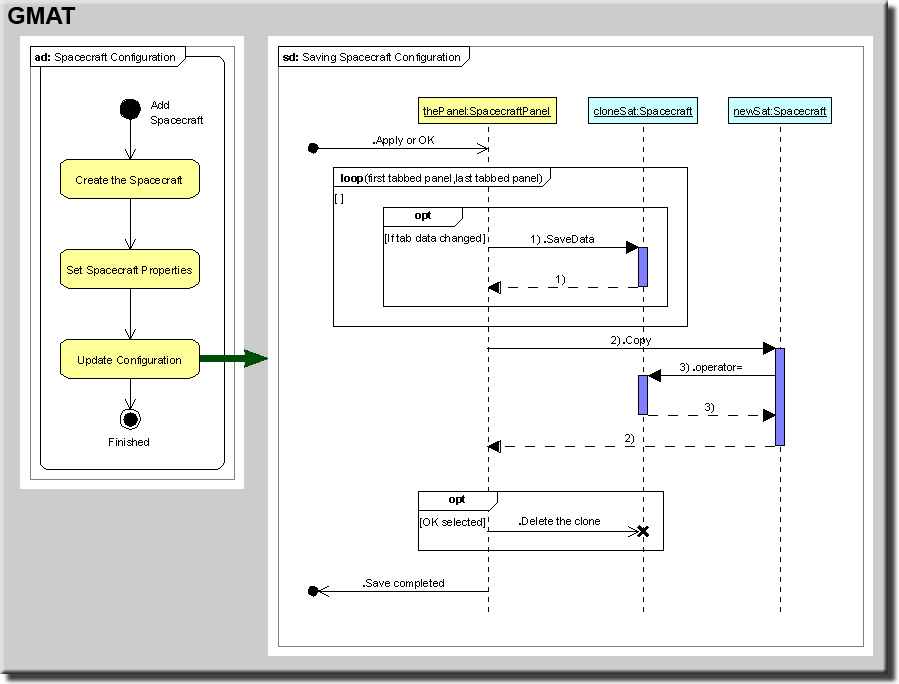
\includegraphics[450,342]{Images/SpacecraftSave.png}
\caption{\label{figure:SavingResource}Configuration Example: Saving the Spacecraft}
\end{center}
\end{figure}

The final step in the spacecraft configuration process is saving the updated data into the
configuration.  That process is shown in Figure~\ref{figure:SavingResource}.

The Spacecraft Panel has several tabbed subpanels.  The SpacecraftPanel begins the save process by
calling each of these subpanels in turn, setting the corresponding Spacecraft data one subpanel at a
time on the locally cloned Spacecraft.  Once all of the subpanels have synchronized their data with
the clone, the copy constructor of the configured Spacecraft is called with the cloned Spacecraft as
the input argument.  This action updates the configured Spacecraft, completing the save action.

There are two buttons on the Spacecraft Panel that can be used to perform the save action.  The
button labeled ``Apply'' saves the updated data to the configured object and leaves the Spacecraft
Panel open for further user manipulation.  The ``OK'' button saves the data and closes the panel.
The latter action destroys the instance of the panel.  Since the panel is going out of scope, the
cloned Spacecraft must also be deleted, as is shown in the figure.

\subsection{Configuring Commands}\index{Model!Commands}

The previous paragraphs describe the interactions between core GMAT components and the internal
message passing that occurs when a component of a GMAT Model is configured for use.  The following
paragraphs describe the analogous configuration for the commands in the Mission Control Sequence.

\begin{figure}[htb]
\begin{center}
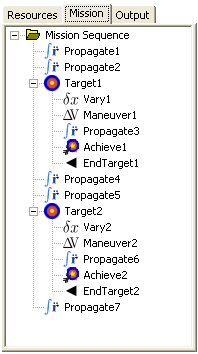
\includegraphics[99,177]{Images/MissionTree.png}
\caption{\label{figure:MissionTree}The Mission Tree in GMAT's GUI}
\end{center}
\end{figure}

The Mission Control Sequence is shown in the GMAT GUI on the tab labeled ``Mission,'' shown for a
modified Hohmann transfer problem\footnote{The modification made here is along the transfer
trajectory from the initial orbit to the final orbit.  The spacecraft in this example is propagated
through one and a half orbits on the transfer trajectory, rather than the typical half orbit needed
for the problem.} in Figure~\ref{figure:MissionTree}.  The sequence is shown as a hierarchical tree
of commands.  Each level of the hierarchy is a separate list of commands.  The top level list is the
main control sequence.  Commands that branch from this list are shown indented one level from this
sequence.  Commands branching off of these commands are indented an additional level\footnote{In
some cases sequences of similar commands are also indented to simplify the display of the Mission
Control Sequence.}.  This process continues until all of the commands in the sequence are
incorporated into the tree structure.

The Mission Control Sequence shown in the figure consists of seventeen commands, grouped as seven
commands in the main (i.e. top level) sequence, five additional commands branched off of this
sequence to perform one set of maneuver targeting, and an additional five commands to perform
targeting for a second maneuver.  The main sequence of commands shown here is the sequence Propagate
-- Propagate -- Target -- Propagate -- Propagate -- Target -- Propagate.  The Target commands are
used to tune the maneuvers at each end of the transfer orbit by applying the command sequence Vary
-- Maneuver -- Propagate -- Achieve -- EndTarget.  The inner workings of these commands is beyond
the scope of this chapter; the important thing to observe at this point is the sequencing of the
commands, and the presentation of this sequencing to the user by way of GMAT's GUI.

The tree shown in the GUI is populated by traversing the linked list of commands comprising the
Mission Control Sequence.  Each node of the Mission Tree is an instance of the class
MissionTreeItemData.  This class includes a pointer to the corresponding GmatCommand object in the
Mission Control Sequence.  When GMAT needs to build or refresh the Mission Tree, it accesses the
first node in the Mission Control Sequence and creates a corresponding MissionTreeItemData instance.
That instance is passed the pointer to the GmatCommand, and uses that command pointer to configure
its properties in the tree.  GMAT then asks for the next node in the sequence, and repeats this
operation until the tree is fully populated.

Some GmatCommands are derived from a subclass named BranchCommand.  These commands manage child
linked lists, like the ones shown for the target commands in the figure.  When the GUI encounters a
BranchCommand derivative, it indents the nodes displayed on the Mission Tree to indicate this nested
level for the child sequence of the branch command.  All of the commands that allow this type of
nesting are terminated with a corresponding ``End'' command -- for this example, the Target command
terminates the targeting child sequence when it encounters an EndTarget command.

Users interact with the Mission Control Sequence either through GMAT's scripting interface, or
through manipulations made in the GUI.  Manipulations made while scripting are pretty
straightforward; they consist of editing a script file of commands and then instructing GMAT to
parse this script.  This process will be described later.  Figure~\ref{figure:CommandConfig} shows
the steps a user takes when adding a command to the Mission Control Sequence from the GUI.

\begin{figure}[H]
\begin{center}
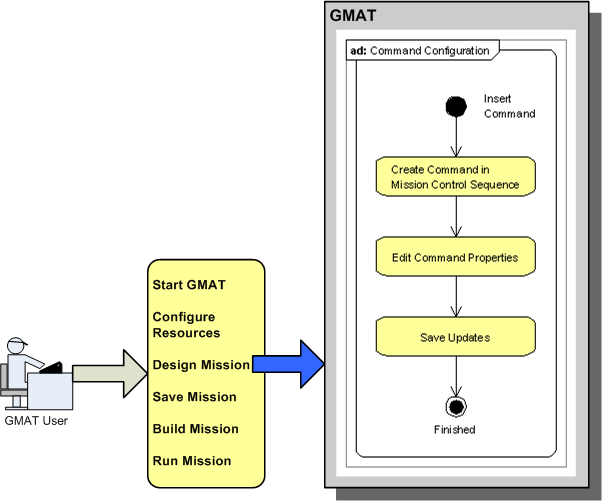
\includegraphics[301,251]{Images/GMAT_ConfigureCommand.png}
\caption{\label{figure:CommandConfig}Configuration Example: A Mission Control Sequence Command}
\end{center}
\end{figure}

The Mission Control Sequence is a doubly linked list of objects that describes the sequence of
actions that GMAT will run when executing a mission.  Each node in the linked list is an object
derived from the command base class, GmatCommand, as is described in Chapter~\ref{chapter:Commands}.
 Since GmatCommand objects are doubly linked in the list, each command has a pointer to its
predecessor and to the next command in the list.  When a user decides to add a command to the
Mission Control Sequence, a node in the Mission tree is selected and right clicked (or
control-clicked on the Macintosh).  This action opens a context menu with ``Insert Before'' and
``Insert After'' submenus as options.  The ``Before'' and ``After'' selections here refer to the
location of the new command.  The user selects the desired command type from the submenu, and the
requested command is added to the Mission Control Sequence in the specified location.  This set of
actions corresponds to the first block in the activity diagram, labeled ``Create Command in Mission
Control Sequence.''

Most of the commands in GMAT require additional settings to operate as the user intends -- for
example, Propagate commands require the identity of the propagator and spacecraft that should be
used during propagation.  The second block in the figure, ``Edit Command Properties,'' is launched
when the user double clicks on a command.  This action opens a command configuration panel designed
to help the user configure the selected command.  The user edits the command's properties, and then
saves the updates back to the command object by pressing either the ``Apply'' or ``OK'' button on
the panel.  This action is performed in the ``Save Updates'' block in the figure, and is the final
step a user takes when configuring a command.

Each of these high level actions can be broken into a sequence of steps performed between the core
elements of GMAT, as is described in the following paragraphs, which describe the interactions
followed to add a Maneuver command to the Mission Control Sequence.

\subsubsection{\label{section:CommandCreation}Creating a Maneuver Command}

Figure~\ref{figure:ManeuverCreation} shows the process followed when a Maneuver command is created
and inserted following an existing command from the GMAT GUI.  The process starts when the user
selects a command on the mission tree, right clicks it, and chooses the ``Insert After'' option
from the resulting context menu.  The resulting submenu contains a list of available commands; the
following actions occur when the user selects ``Maneuver'' from this list.

\begin{landscape}
\begin{figure}[htb]
\begin{center}
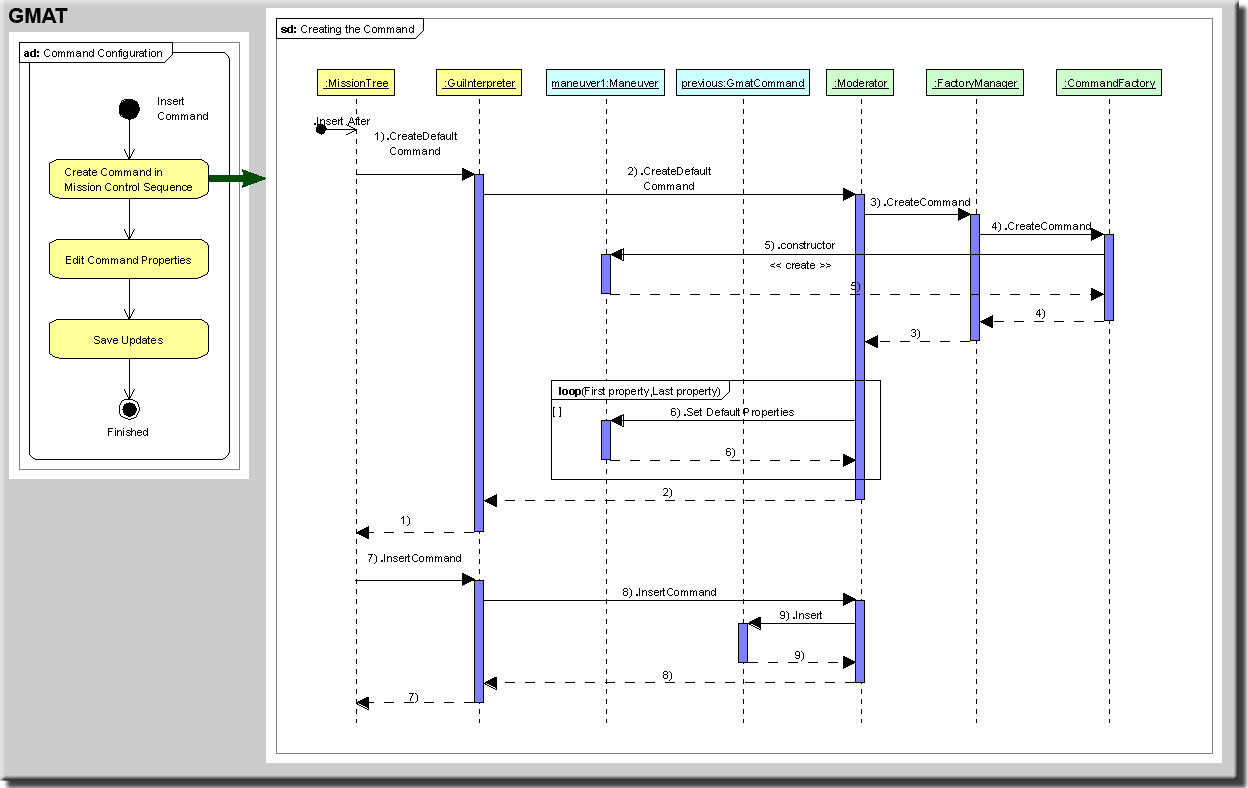
\includegraphics[560,355]{Images/ManeuverCreation.png}
\caption{\label{figure:ManeuverCreation}Command Creation Example: Creating a Maneuver Command}
\end{center}
\end{figure}
\end{landscape}

Maneuver command creation starts when the MissionTree\footnote{Here, and throughout this document,
specific instances of singleton classes are referred to by the class name -- ``MissionTree'' in this
case.  When the class or user experience of the instance is discussed, it will be referred to
 less formally -- ``mission tree'', for example.  So as an example of this style, we might discuss
the user selecting an object on the mission tree in the GUI, which causes the MissionTree to perform
some action.} object sends a request to the GuiInterpreter for a new Maneuver command instance. The
GuiInterpreter sends the request to the Moderator, which sends the request to the FactoryManager.
The FactoryManager finds the factory that creates Maneuver commands, and asks that factory for an
instance of the Maneuver command.  The resulting instance is returned from the factory, through the
FactoryManager, to the Moderator.  The Moderator sets some default data on the command, and then
returns the command pointer to the GuiInterpreter. The GuiInterpreter passes the command pointer to
the MissionTree.

Each node in the MissionTree includes a data member pointing to the corresponding command in the
Mission Control Sequence.  This structure simplifies the interactions between the GUI and the engine
when a user makes changes to the Mission Control Sequence.  Since the MissionTree already has a
pointer to the command preceding the new Maneuver command, it has all of the information needed to
request that the new command be added to the Mission Control Sequence.  The new Maneuver command is
added to the Mission Control Sequence from the MissionTree.  The MissionTree passes two pointers
through the GuiInterpreter to the Moderator: the first pointer identifies the command selected as
the command preceding the new one, and second pointer is the address of the new Maneuver command.
The Moderator passes these two pointers to the head of the Mission Control Sequence using the
``Insert'' method. This method searches the linked list recursively until it finds the node
identified as the previous command node, and adds the new command immediately after that node in the
list, resetting the linked list pointers as needed.  This completes the process of adding a command
to the Mission Control Sequence.

\subsubsection{\label{section:CommandConfiguration}Configuring and Saving the Maneuver Command}

When a new command is added to the Mission Control Sequence, it is incorporated into the sequence
with default settings selected by the Moderator.  Most of the time, the user will want to edit
these settings to match the requirements of the mission being modeled.  Command configuration is
performed using custom panels designed to display the properties users can set for each command.
Figure~\ref{figure:ManeuverConfigPanel} shows the panel that opens when a user double clicks a
maneuver command -- like the one created in the example described above -- in the mission tree.

\begin{figure}[htb]
\begin{center}
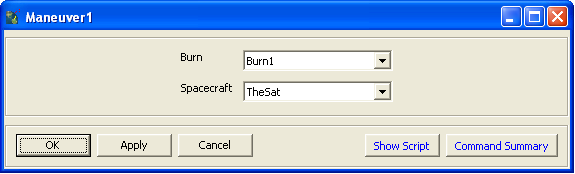
\includegraphics[288,88]{Images/ManeuverPanel.png}
\caption{\label{figure:ManeuverConfigPanel}The Maneuver Command Configuration Panel}
\end{center}
\end{figure}

The sequence diagram in Figure~\ref{figure:ManeuverConfiguration} shows the top level messages that
are passed when the Maneuver command is configured using this panel.  This view into the command
configuration includes a bit more detail about the GUI messages than was shown in the Spacecraft
configuration presented previously.

\begin{figure}[htb]
\begin{center}
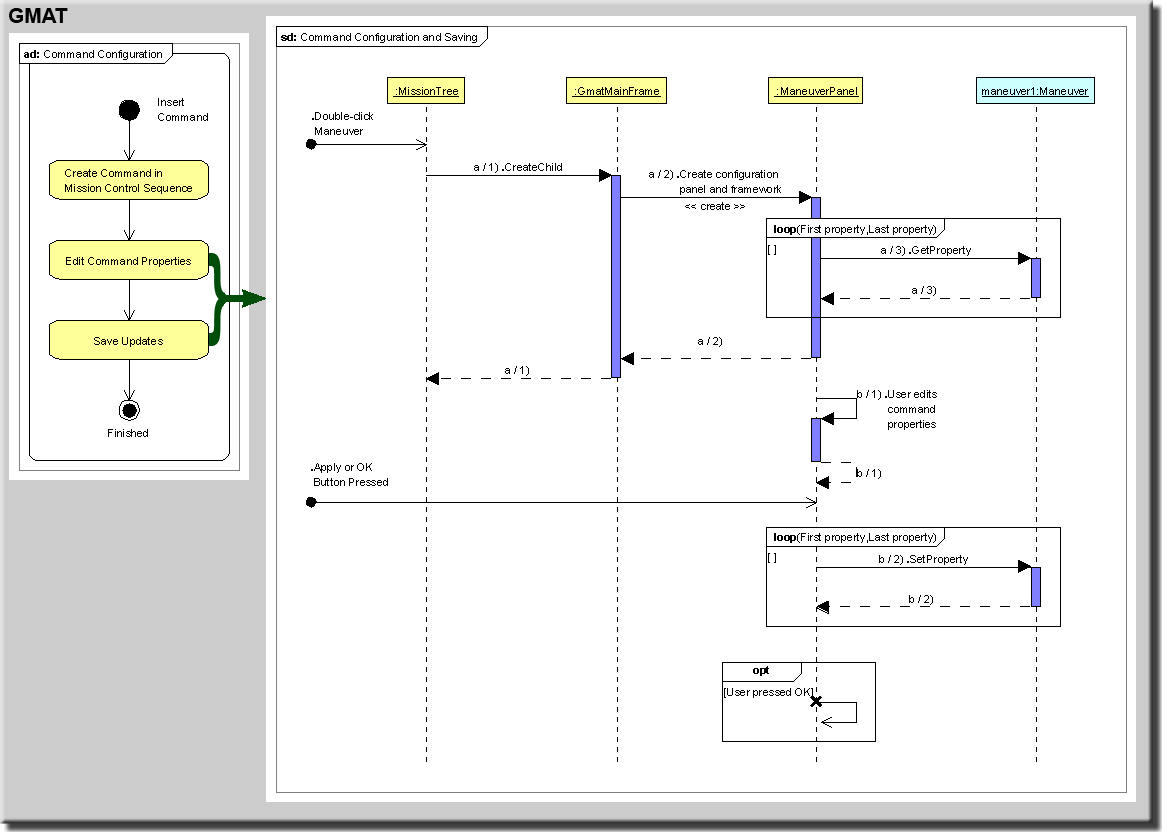
\includegraphics[455,326]{Images/ManeuverConfiguration.png}
\caption{\label{figure:ManeuverConfiguration}Command Configuration Example: Configuring the Maneuver
Command}
\end{center}
\end{figure}

The configuration process starts when the user double clicks on the command in the mission tree. 
The double click action sends a message to the MissionTree requesting the configuration panel for
the
selected node in the tree.  The MissionTree finds the item data, and sends that data to the main
GMAT window, called the GmatMainFrame, asking for a new child window configured to edit the
properties of the command contained in the item data.  The GmatMainFrame creates the child window
and displays it for the user.

More concretely, if the user double clicks on the Maneuver command created in the preceding
section, the tree item data for that maneuver command is passed from the MissionTree to the
GmatMainFrame.  The configuration window that should result from this action for display in the GUI
needs to contain the panel designed to match the underlying object that is being configured -- in
this case, a Maneuver command.  The GmatMainFrame uses the tree item data passed to it to determine
the type of panel needed by the child window during its creation. For this example, the
GmatMainFrame determines that the panel that is needed should be a ManeuverPanel because the tree
item data includes a pointer to a Maneuver command.  Accordingly, the GmatMainFrame creates an
instance of the ManeuverPanel class, and passes that panel to the child window.  The child window
receives the panel and places it into the corresponding container in the window.

Finally, the child window uses the command pointer in the tree item data to access the command and
determine the current values of its internal properties.  These data are collected from the command
and passed to the corresponding GUI components so that the user can see the current settings. Once
these data fields have been populated, the child window is displayed on the GUI, giving the GUI a
new window like that shown in Figure~{figure:ManeuverConfigPanel}.  This completes the top portion
of
the sequence shown in Figure~\ref{figure:ManeuverConfiguration}.

Once the panel is shown on the GUI, the user makes changes to the settings for the command on the
new panel.  When the settings match the needs of the mission, the user clicks on either the ``OK''
or ``Apply'' button.  This action makes the ManeuverPanel update the Maneuver command with the new
settings.  If the user pressed the OK button, the child window also passes a message to GMAT
indicating that the user is finished with the window.  When that message is processed, the child
window is closed in the GUI.

\subsection{Model and Mission Persistence: Script Files}\index{Model!Scripts}

GMAT saves configuration data in files referred to as script files.  The details of the script file
parsing can be found in Chapter~\ref{chapter:ScriptRW}.  The following paragraphs provide an
overview of these processes.

The GMAT script files can be thought of as a serialized text view of the configured objects and
Mission Control Sequence constructed by the user to model spacecraft.  GMAT provides a subsystem,
controlled by the ScriptInterpreter, that manages reading and writing of these files.  All of these
script files are ASCII based files, so they can be edited directly by users.

\lstset{numbers=left}
\lstinputlisting[caption={A Basic GMAT Script File},label=listing:BasicScript,firstnumber=1]
{script/BasicScript.script}
\lstset{numbers=none}

Listing~\ref{listing:BasicScript} shows a simple script that propagates a spacecraft for
approximately 7~days, plotting the Cartesian components of the velocity against the spacecraft's X
coordinate value.  Details of all of these settings can be found in the User's
Guide\cite{userGuide}. This script just serves as an example for the discussion that follows.

All objects that are created as configured resources from the GUI are stored in the script files
using the keyword ``Create''.  In the script shown here, there are four resources: a Spacecraft
named ``sat1'', a ForceModel named ``fm'', a Propagator (actually an instance of the PropSetup
class) named ``prop'', and an XYPlot Subscriber named ``posvel''.  Each of these resources is used
when running the mission.

In GMAT, each resource can have one or more data members that users can set.  These resource
properties are initialized to default settings.  Users can override the values of these properties.
In the GUI, this action is performed by editing data presented on the panels for the resources.
Properties are changed in the script file by assigning new values to the properties by name; for
example, in the sample script, the Spacecraft's semimajor axis is changed to 10000.0 km on the fifth
line of script:

\begin{lstlisting}
sat1.SMA = 10000.0
\end{lstlisting}

\noindent The script shown here is a script as it might be entered by a user.  Only the lines that
override default property values are shown, and the lines are written as simply as possible.  The
full set of object properties can be examined by writing this object to a script file.  When a
Spacecraft -- or any other resource -- is saved, all of the resource properties are written.  In
addition, the keyword ``GMAT'' is written to the file, and the full precision data for the numerical
properties are written as well.  The Spacecraft configured in the script file above is written to
file as shown in Listing~\ref{listing:BasicMissionSpacecraft}.

\lstset{numbers=left,firstnumber=1}
\begin{lstlisting}[caption={Script Listing for a Spacecraft},label={listing:BasicMissionSpacecraft}]
Create Spacecraft sat1;
GMAT sat1.DateFormat = TAIModJulian;
GMAT sat1.Epoch = 21545.000000000;
GMAT sat1.CoordinateSystem = EarthMJ2000Eq;
GMAT sat1.DisplayStateType = Keplerian;
GMAT sat1.SMA = 9999.999999999998;
GMAT sat1.ECC = 0.2499999999999999;
GMAT sat1.INC = 78.5;
GMAT sat1.RAAN = 45;
GMAT sat1.AOP = 7.349999999999972;
GMAT sat1.TA = 0.9999999999999002;
GMAT sat1.DryMass = 850;
GMAT sat1.Cd = 2.2;
GMAT sat1.Cr = 1.8;
GMAT sat1.DragArea = 15;
GMAT sat1.SRPArea = 1;
\end{lstlisting}
\lstset{numbers=none}

\noindent GMAT generates the scripting for resources and commands using a method,
GetGeneratingString(), which is provided in the GmatBase class.  This class provides the
infrastructure needed to read and write object properties through a consistent set of interfaces.
The GetGeneratingString() method uses these interfaces when writing most user objects and commands
to script.  Derived classes can override the method as needed to write out class specific
information.
When GMAT saves a model to a script file, it tells the ScriptInterpreter to write a script file with
a given name.  The ScriptInterpreter systematically calls GetGeneratingString() on each object in
the configuration and sends the resulting serialized form of each object to the script file.  Once
all of the objects in the configuration have been saved, GMAT takes the first command in the Mission
Control Sequence and calls its GetGeneratingString() method, writing the resulting text to the
script file.  It traverses the command list, writing each command in sequential order.

Script reading inverts this process.  When a user tells GMAT to read a script, the name of the
script file is passed to the ScriptInterpreter.  The ScriptInterpreter then reads the file, one
logical block\footnote{A ``logical block'' of script is one or more lines of text sufficiently
detailed to describe a single action taken in GMAT.  Examples include creation of a resource,
setting of a single parameter on a resource, or adding a command to the Mission Control Sequence.}
at a time, and constructs and configures the scripted objects following a procedure similar to that
described above for actions taken from the GUI.

Details of script processing can be found in Chapter~\ref{chapter:ScriptRW}.

\subsection{\label{section:SandboxMCSExecution}Running a Mission}\index{Model!Running}

Once a user has configured a model in GMAT, the model is ready to be run.  The configuration has
been populated with all of the resources needed for the run, and the resources have been configured
to match the needs of the analyst.  The Mission Control Sequence has been entered and configured to
meet the needs of the mission.  All that remains is the actual running of the model encoded in these
elements.

Figure~\ref{figure:RunningBasicScript} shows the sequence followed when a mission is executed in
GMAT.  The figure shows the sequence as initiated in the GUI.  The user chooses to run the mission
by pressing the ``Run'' button on GMAT's toolbar.  This action sends a RunMission message to the
GuiInterpreter, which then calls the Moderator's RunMission() method (Step 1 in the figure).

The Moderator begins by clearing any stale data out of the Sandbox by calling the Sandbox's Clear()
method (Step 2).  This action removes any local copies of objects in the Sandbox that may still
exist from a previous run.  Once the Sandbox has been cleared, the Moderator begins passing
resources into the Sandbox.

The Moderator passes the current Solar System into the Sandbox, and then begins making calls to
ConfigurationManager to get the current set of resources used in the model (Step 3).  The Moderator
passes these resources into the Sandbox (Step 4) by type, starting with coordinate systems, and
proceeding until all of the resources have been passed into the Sandbox.  The Sandbox receives each
resource as it is passed in and makes a copy of that resource by calling its Clone() method (Steps 5
and 6).  The Sandbox stores these local clones by name in its local object map.  The local object
map contains the objects that are manipulated during a run; the configured objects are not used when
running the mission.

After the configured objects have been passed into the Sandbox, the Moderator sends the head node of
the Mission Control Sequence to the Sandbox\footnote{Commands are not cloned into the Sandbox at
this writing.  A future build of GMAT may require cloning of commands as well as resources, so that
the system can support multiple Sandboxes simultaneously.  The system is designed to allow this
extensibility when needed.} (Step 7).  This sets the Sandbox's internal sequence pointer to the
first command in the Mission Control Sequence (Step 8), completing steps needed to begin work in the
Sandbox.

\label{section:SandboxInitializationOverview}The Moderator has completed the bulk of its work for
the run at this point.  The next action taken is a call from the Moderator to the Sandbox,
instructing it to initialize itself (Step 9).  When the Sandbox receives this instruction, it begins
initializing the local objects.  Each object is queried for a list of referenced objects that need
to be set, and the Sandbox finds these objects in the local object store and sets each one on the
requesting object (Step 10, performed iteratively through all of the objects).  After the object
initialization, the Sandbox walks through the Mission Control Sequence node by node, passing each
command a pointer to the local object map and then calling the Command's Initialize method, giving
each command the opportunity to set up data structures needed to execute the Mission Control
Sequence  (Step 11, performed iteratively through the Mission Control Sequence).  If initialization
fails at any point during this process, the Sandbox halts the initialization process and reports the
error to the Moderator.

Once initialization is complete, the Sandbox reports successful initialization to the Moderator.  At
this point the Moderator sends an Execute() message to the Sandbox (Step 12).  The Sandbox responds
by calling the Execute() method on the first command in the Mission Control Sequence (Step 13).  The
command executes this method, manipulating objects in the local object map  (Step 14) and sending
data to GMAT's Publisher (Step 15) based on the design of each command.  When data is passed to the
Publisher, it passes the data on to each Subscriber (Step 16), producing output that the user can
view to monitor the mission as it executes, or to process after the mission has finished running.

When the first command completes execution, the Sandbox asks for the next node to execute in the
Mission Control Sequence, and repeats this process on the second node.  The process continues,
calling node after node in the Mission Control Sequence until the final command has been executed.

\begin{figure}[H]
\begin{center}
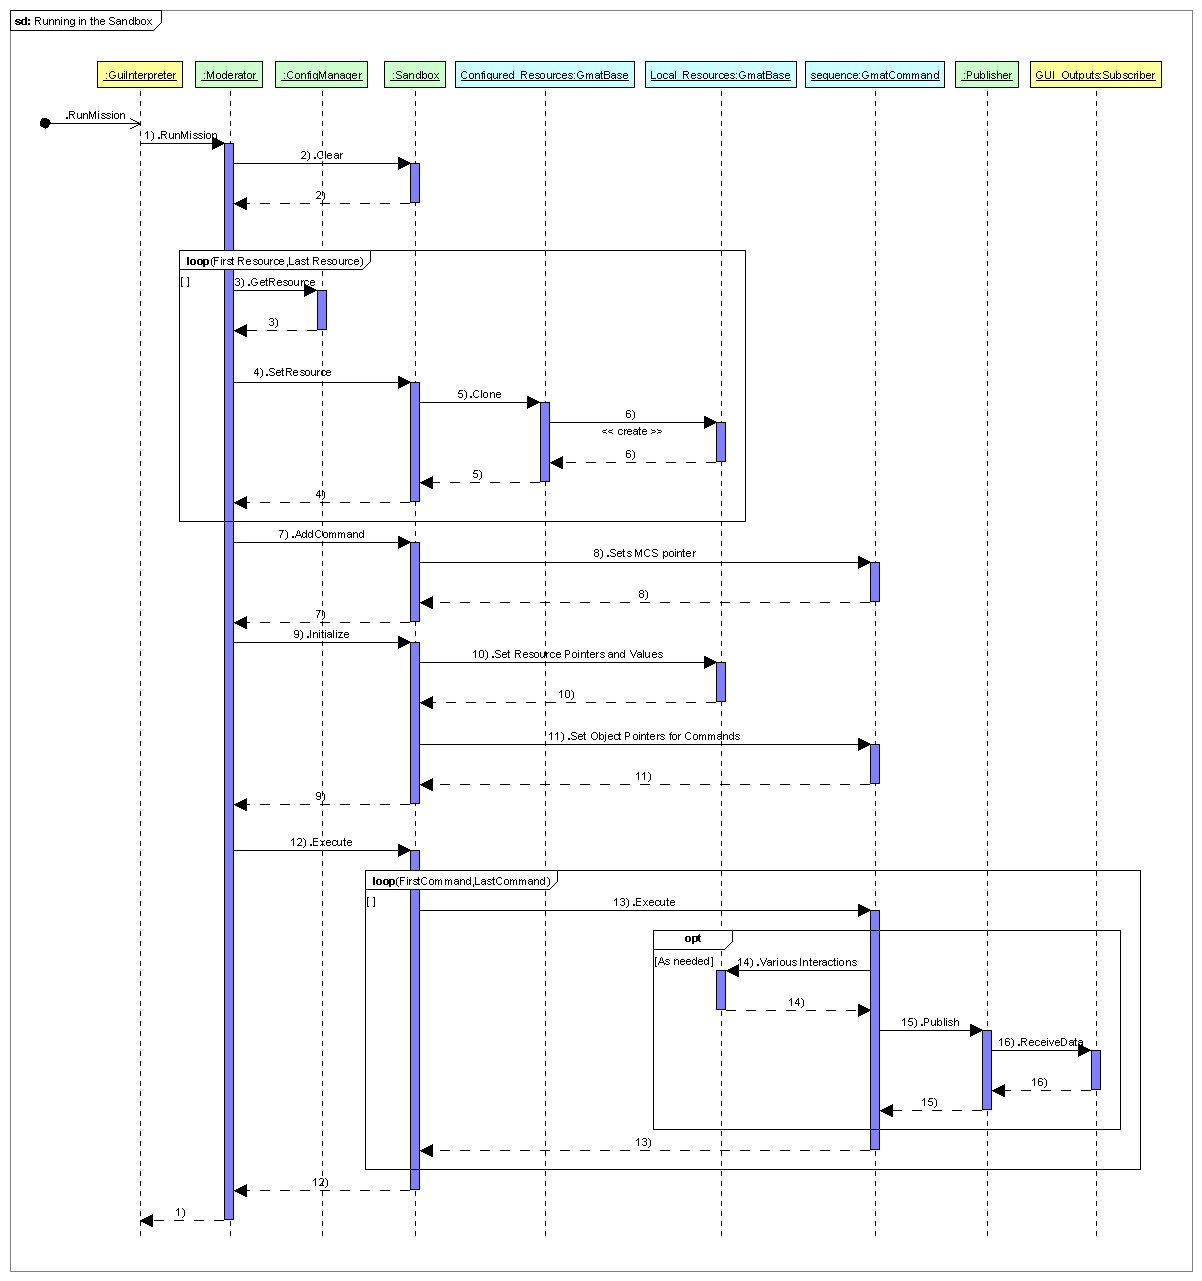
\includegraphics[455,485]{Images/RunningintheSandbox.png}
\caption{\label{figure:RunningBasicScript}The Sequence followed to Run a Mission}
\end{center}
\end{figure}

\begin{figure}[H]
\begin{center}
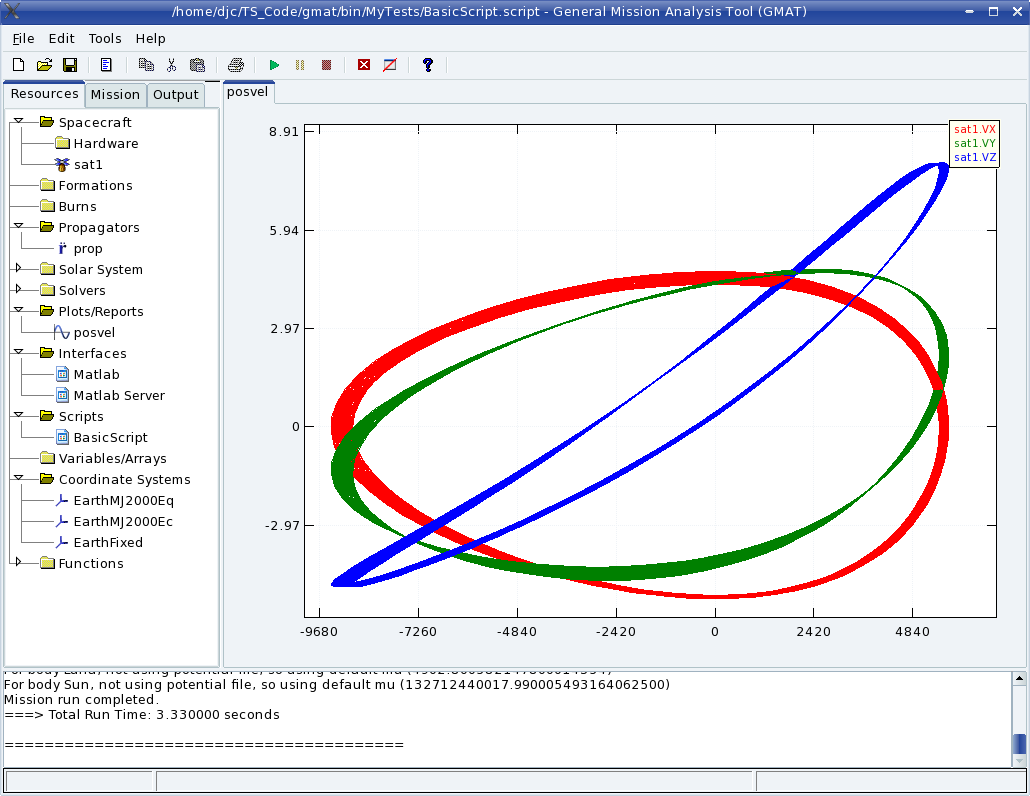
\includegraphics[455,352]{Images/BasicMissionRunLinux.png}%
\caption{\label{figure:BasicScriptOutput}Results of the Script Example, Run on Linux}%
\end{center}
\end{figure}

Once the final command has executed, the Sandbox sends a message to the Mission Control Sequence
stating that the run has completed execution, and control is returned to the Moderator from the
Sandbox.  The Moderator returns control to the GuiInterpreter, which returns control, through the
GUI, to the user, completing the mission run.  Figure~\ref{figure:BasicScriptOutput} shows the
results of this sequence when executed for the script shown in Listing~\ref{listing:BasicScript}.

\section{Summary}

This completes the presentation of the overview of GMAT's architecture.  In this chapter we have
discussed the basic architecture for GMAT, presented an overview of the arrangement of the
components of the system that we will build upon in upcoming chapters, and presented a programmatic
description of the workflow of three common tasks performed in GMAT: Starting the system, Creating
resources and comments for a spacecraft mission, and running that mission.

The next few chapters will present, in some detail, descriptions of each of the components of the
Engine package, followed by sections describing the infrastructure used for the Resources and
Commands, and then the design features of these elements.

\part{Engine Components}
\thispagestyle{empty}

% $Id: ExecComponents.tex,v 1.1 2008/01/31 18:04:16 dconway Exp $
%\chapter{\label{chapter:Engine}Components of the GMAT Engine}
%\chapauthor{Darrel J. Conway}{Thinking Systems, Inc.}

\setcounter{footnote}{0}

\section*{Overview of Chapters~\ref{chapter:Moderator} through \ref{chapter:Publisher}}

Mission modeling is performed in GMAT through the core numerical engine designed for the system.
This part of the architectural specification describes the classes that make up the core engine
components: the Moderator, the Factory Manager, the Configuration Manager, the Publisher, and
Sandboxes.  The purpose of each of these components is summarized in
Table~\ref{table:EngineComponents}.

\begin{table}[H]
\begin{center}
\caption{\label{table:EngineComponents}Key Elements of the GMAT Engine}
\setlength\extrarowheight{2pt}
\begin{tabular}{|p{1.4in}|p{1in}|p{3.4in}|}
\hline
Component & Notes & Description \\
\hline
\hline
Moderator & Singleton & Controls the program flow in the Engine.\\
Factory Manager & Singleton & Responsible for the creation of objects and Mission Control
Sequence commands used in the flight dynamics model.\\
Configuration Manager & Singleton & Stores and retrieves user objects created by the
Factory Manager.\\
Publisher & Singleton & Passes data generated during a run to the Subscribers that present these
data to users.\\
Sandbox & Multiple copies allowed\footnotemark & The component that manages initialization and
execution of the Mission Control Sequence when a mission is run.\\
\hline
\end{tabular}
\end{center}
\end{table}
\footnotetext{While GMAT is designed to allow more than one Sandbox, the current implementation only
uses a single Sandbox.}

\section*{Contents of the Chapters}

Each component of the engine is described in a separate chapter, structured on the following
outline:

\begin{description}
\item[Overview]

The introductory text for each chapter contains an overview of the component and its role in the
GMAT engine.

\item[Design Principles]

This section describes the motivation behind the component, along with the principles followed while
designing it.  It includes a description of patterns or other criteria used in the component design,
the roles and responsibilities handled by the component, and other design features that will help
you understand how the component fits into the GMAT engine.

\item[Design]

The design section presents the design for the component.  It starts with the class diagram
for the component, followed by descriptions of representative methods and attributes of the class
selected to help you understand its implementation.  It also provides an explanation of how the
class satisfies the roles and responsibilities identified in the preceding section, through the use
of activity and sequence diagrams.  Sometimes the details of these descriptions are better placed in
other portions of the design specification; when that happens, a summary is provided in the chapter
along with a reference to the detailed description.

\item[Usage and Modification]

This section of the chapter provides additional tips about how to use or change the component, and
includes text describing best practices for working with it.
\end{description}

% \section{\label{ModeratorOverview}The Moderator}
% 
% The core executive for GMAT is the Moderator.  The Moderator controls program flow, creating
% components through the factory manager that are then managed in the configuration manager and
%using
% these components to model missions in a sandbox.
% 
% \begin{figure}[htb]
% \begin{center}
% 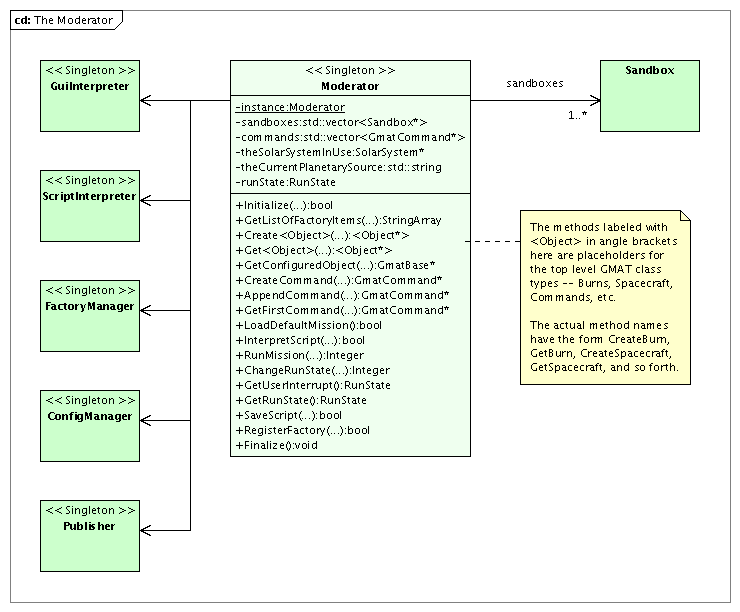
\includegraphics[370,346]{Images/TheModerator.png}
% \caption{The Moderator in its Environment}
% \label{figure:ModeratorClassDiagram}
% \end{center}
% \end{figure}
% 
% Figure ~\ref{figure:ModeratorClassDiagram} shows the Moderator, the classes it interacts with, and
% many of its key internal structures.  The interactions between the Moderator and other elements of
% GMAT's engine were presented in Chapter~\ref{chapter:TopLevel}.  The sequence diagrams presented
% there describe at a high level the interfaces to the Moderator and their usage when constructing a
% model.  The methods shown in Figure~\ref{figure:ModeratorClassDiagram} present these interfaces in
% more detail.  The following paragraphs describe these interfaces and the internal data members
%used
% by the Moderator.
% 
% \subsection{\label{section:ModeratorAttributes}Attributes and Methods of the Moderator Class}
% 
% The Moderator is a large class.  The following lists of attributes and methods provide an overview
% of the features of the class.  Interested readers should browse the code in the
% base/executive/Moderator.cpp and base/executive/Moderator.hpp, or generate the full API using
% Doxygen\cite{doxygen}, to see the full implementation details of the Moderator.
% 
% \subparagraph{\textit{Class Attributes}}
% 
% The key data members of the Moderator are the pointers to other engine elements and some core
%model
% components, as are listed here:
% 
% \begin{itemize}
% \item \textbf{static Moderator *instance}: The singleton instance of the Moderator.
% \item \textbf{std::vector<Sandbox*> sandboxes}: The sandboxes managed by the moderator.
% \item \textbf{std::vector<GmatCommand*> commands}: The Mission Control Sequences managed by this
% Moderator.  The current implementation manages one Mission Control Sequence per Sandbox.
% \item \textbf{static GuiInterpreter* theGuiInterpreter}: A pointer to the GuiInterpreter
%singleton.
% \item \textbf{static ScriptInterpreter* theScriptInterpreter}: A pointer to the ScriptInterpreter
% singleton.
% \item \textbf{ConfigManager* theConfigManager}: A pointer to the configuration manager singleton.
% \item \textbf{FactoryManager* theFactoryManager}: A pointer to the factory manager singleton.
% \item \textbf{FileManager* theFileManager}: A pointer to the file manager, a helper class used to
% manage file processing.
% \item \textbf{Publisher* thePublisher}: A pointer to the Publisher singleton.
% \item \textbf{SolarSystem* theSolarSystemInUse}: A pointer to the SolarSystem instance used when
% running a mission.
% \item \textbf{std::string theCurrentPlanetarySource}: An identifier for the current default
% planetary ephemerides source.
% \item \textbf{RunState runState}: The current state of the engine.
% \end{itemize}
% 
% \subparagraph{\textit{Engine Execution Methods}}
% 
% The methods implemented in the Moderator are broken into two categories: those used to run the
% engine, and those used to manipulate the configured objects and commands.  The following list
% describes the methods that fall into the first group.
% 
% \begin{itemize}
% \item \textbf{bool Initialize(bool isFromGui = false)}: Initializes the Moderator at the start of
% the program.  The argument to this method, isFromGui, is set to true if the Moderator was created
%in
% GMAT's GUI; otherwise, it should be set to false.  Moderator initialization is used to create the
% other singleton classes used in GMAT, some default model elements, and, when launched from the
%GUI,
% a default Mission Control Sequence.
% \item \textbf{void Finalize()}: Cleans up memory when the GMAT engine is closed down.
% \item \textbf{StringArray GetListOfFactoryItems(Gmat::ObjectType type)}: Returns a list of item
% object types, identified by generic type, that can be created in the Factory subsystem.  This
%method
% is used to determine the types of concrete objects that can be created of a given abstract type --
% for example, the list of available GmatCommands can be generated by calling this method and
% requesting the list of Gmat::COMMAND items.
% \item \textbf{bool LoadDefaultMission()}: Sets up the default mission that appears when GMAT is
% started.
% \item \textbf{void ClearAllSandboxes()}: Instructs each sandbox to clear its data and local object
% maps.
% \item \textbf{Integer RunMission(Integer sandboxNum = 1)}: This is the entry point for running a
% mission in GMAT.  The method loads the configured objects into the Sandbox, sets the Mission
%Control
% Sequence, instructs the Sandbox to initialize itself, and then to execute the control sequence.
% \item \textbf{Integer ChangeRunState(const std::string \&state, Integer sandboxNum = 1)}: Sets
% GMAT's RunState to IDLE, PAUSED, or RUNNING, based on the state description contained in the state
% string.  The sandboxNum parameter is not yet used; when multiple Sandboxes are implemented, each
% Sandbox will have its own RunState.
% \item \textbf{RunState GetUserInterrupt()}: Retrieves the RunState from the Modeartor so that the
% Sandbox can take appropriate actions in response to state changes generated by the user.  This
% method is used when the Sandbox polls the Moderator for user messages, and provides a time slice
%for
% the GUI to process user actions like selection of the Stop or Pause buttons on the toolbar.
% \item \textbf{RunState GetRunState()}: Returns the current RunState from the Moderator.
% \item \textbf{bool InterpretScript(const std::string \&filename, bool readBack, const std::string
% \&newPath)}: This method clears the current configuration and Mission Control Sequence from
%memory,
% and then  reads in and parses a script file, building a new configuration and Mission Control
% Sequence based on the contents of the script file.
% \item \textbf{bool SaveScript(const std::string \&filename, WriteMode mode = Gmat::SCRIPTING)}:
% Writes the current configuration and Mission Control Sequence to a script file, formatted in the
% mode specified by the mode flag.
% \item \textbf{std::string GetScript(WriteMode mode = Gmat::SCRIPTING)}: Writes the current
% configuration and Mission Control Sequence to a string, formatted in the mode specified by the
%mode
% flag.
% \item \textbf{Integer RunScript(Integer sandboxNum = 1)}:  Runs the current mission in the
%specified
% Sandbox.
% \end{itemize}
% 
% \subparagraph{\textit{Configured Object and Command Methods}}
% 
% The Moderator has methods to handle object and command creation for all of the user accessible
% components of the flight dynamics model, and to access these components after they have been
% created.  These facilities are used by the Interpreters during model configuration.  Future
%releases
% may also provide access to these methods from the Sandbox during a run to support object creation
% during a mission.
% 
% The configured objects are handled by type in the current implementation.  That means that there
%are
% methods with the names CreateSpacecraft and GetSpacecraft for Spacecraft objects, CreateBurn and
% GetBurn for Burn objects, and so forth for all of the configured objects created or accessed
%through
% the Moderator.  The methods used for these functions are all similar in form, so for the purposes
%of
% this chapter, they are referenced using the markers <Object> and <Object*> in the following list.
% 
% The methods used by the Moderator to create and access objects and commands are listed here:
% 
% \begin{itemize}
% \item \textbf{<Object*> Create<Object>(const std::string \&type, const std::string \&name)}:
%Creates
% an object of a given type, and assigns the specified name to that object.
% \item \textbf{<Object*> Get<Object>(const std::string \&name)}: Retrieves a named object from the
% configuration.
% \item \textbf{GmatCommand* InterpretGmatFunction(const std::string \&functionFilename)}: Builds a
% command list for a GmatFunction\footnote{GmatFunctions are not yet fully implemented.}.
% \item \textbf{GmatCommand* CreateCommand(const std::string \&type, const std::string \&name, bool
% \&retFlag)}: Creates a GmatCommand and returns it.  This method does not add commands created with
% it to the Mission Control Sequence.
% \item \textbf{GmatCommand* AppendCommand(const std::string \&type, const std::string \&name, bool
% \&retFlag, Integer sandboxNum = 1)}: Creates a GmatCommand, appends it to the Mission Control
% Sequence, and returns it.
% \item \textbf{GmatCommand* AppendCommand(GmatCommand *cmd, Integer sandboxNum = 1)}: Appends an
% existing GmatCommand to the Mission Control Sequence.
% \item \textbf{GmatCommand* GetFirstCommand(Integer sandboxNum = 1)}: Returns the head of the
%Mission
% Control Sequence for the specified Sandbox.
% \item \textbf{GmatCommand* DeleteCommand(GmatCommand *cmd, Integer sandboxNum = 1)}: Removes a
% command from the Mission Control Sequence linked list.  The removed command is returned to the
% caller for processing or deletion; the method does not call the destructor on the command.
% \item \textbf{bool InsertCommand(GmatCommand *cmd, GmatCommand *prevCmd, Integer sandboxNum~=~1)}:
% Inserts a command into the Mission Control Sequence.
% \item \textbf{GmatBase* GetConfiguredObject(const std::string \&name)}: Retrieves a configured
% object from the configuration.
% \item \textbf{bool ClearResource()}: Deletes all objects from the configuration and clears all of
% the Sandboxes.
% \item \textbf{bool ClearCommandSequence(Integer sandboxNum = 1)}: Deletes all commands from the
% Mission Control Sequence for the specified Sandbox.
% \end{itemize}
% 
% \subsection{\label{section:ModeratorStates}States of the Moderator}
% 
% The Moderator tracks the current state of the system using a parameter named runState, which is
%set
% to a value in the RunState enumeration (see Table~\ref{table:RunStateEnum}) defined in the Gmat
% namespace.  The engine states tracked in the Moderator are the IDLE, RUNNING, and PAUSED states.
% The transitions
% 
% \begin{figure}[htb]
% \begin{center}
% 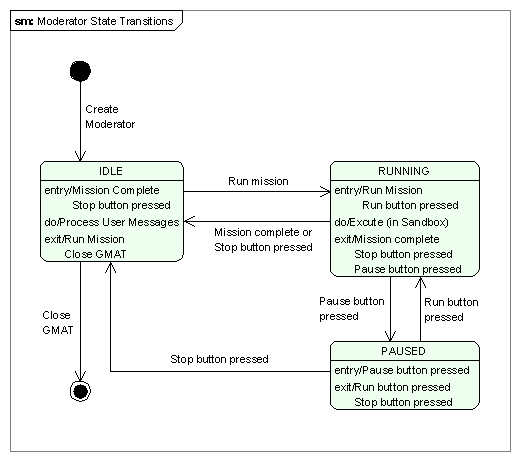
\includegraphics[260,231]{Images/ModeratorStateTransitions.png}
% \caption{State Transitions in the Moderator}
% \label{figure:ModeratorStateTransitions}
% \end{center}
% \end{figure}
% 
% Figure ~\ref{figure:ModeratorStateTransitions} shows the run state transitions tracked by the
% Moderator.  The Moderator is created with the run state set to the IDLE state.  Most of the time,
% the Moderator remains in the IDLE state, processing messages from users and managing the internal
% components of the GMAT engine\footnote{Many of the activities performed by the Moderator in the
%IDLE
% state are described in Chapter~\ref{chapter:TopLevel}.  Additional Moderator interactions with the
% other engine components are described in the appropriate sections of this document.}.
% 
% When a user executes a Mission Control Sequence, the Moderator transitions to the RUNNING state. 
%In
% this state, the Moderator performs very limited processing while the control of the system is
% managed by the sandbox that is running the mission.  The sandbox polls the Moderator for user
% activity at convenient points during the mission run.  This polling allows the Moderator to
%respond
% to user actions that either terminate the mission early or pause the mission.
% 
% If the user presses the pause button on the GUI, the Moderator transitions into the PAUSED state
% when the sandbox polls for state status.  This activity stops the mission run, but maintains data
%so
% that the run can be resumed from the point of the stop.  The user tells the Moderator to resume
%the
% run by pressing the run button on the GUI.  When the Moderator receives the run message, it
% transitions back into the RUNNING state and tells the sandbox to resume the run.
% 
% The user can terminate a run early by pressing the stop button on the GUI during a run.  This
%action
% always causes the Moderator to transition from its current state - either RUNNING or PAUSED --
%into
% the IDLE state.
% 
% \section{\label{section:FactManOverview}The Factory Manager}
% 
% Users configure GMAT by creating and using components designed to model elements or features of a
% satellite system in space.  All of these user elements are created in GMAT's factory subsystem. 
%The
% interface into this system is the FactoryManager, a singleton class that routes requests for
% specific objects into the Factory that is responsible for creating that type of object.  The
%Factory
% classes are described in Chapter~\ref{chapter:Factories}; this section describes how the
% FactoryManager interacts with the Factories and the rest of the GMAT engine to produce requested
% objects.
% 
% \subsection{\label{section:FactManAttributes}Attributes and Methods of the Factory Manager}
% 
% The Factory Manager is a singleton object, and has a fairly simple internal structure, as can be
% seen in the class diagram shown in Figure~\ref{figure:FactManClassDiagram}.  The following lists
% describe the class members shown in the figure.
% 
% \begin{figure}[htb]
% \begin{center}
% 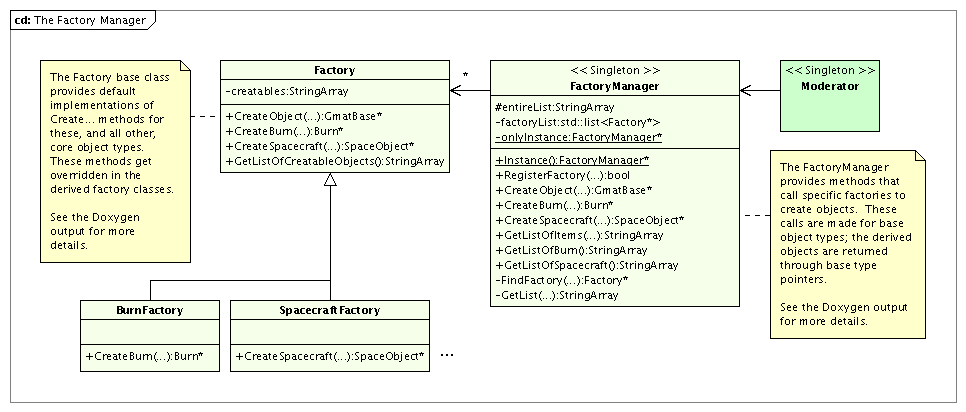
\includegraphics[455,257]{Images/TheFactoryManager.png}
% \caption{The Factory Manager in its Environment}
% \label{figure:FactManClassDiagram}
% \end{center}
% \end{figure}
% 
% \subparagraph{\textit{Class Attributes}}
% 
% The Factory Manager maintains a list of factories, and uses those factories to generate the data
% needed to respond to requests from the rest of GMAT.  There are three data members in the
% FactoryManager:
% 
% \begin{itemize}
% \item \textbf{StringArray entireList}: Array used to store the list of items requested.
% \item \textbf{std::list<Factory*> factoryList}: The array of registered factories managed by the
% Factory Manager.
% \item \textbf{static FactoryManager* onlyInstance}: The singleton pointer for the manager.
% \end{itemize}
% 
% \subparagraph{\textit{Methods}}
% 
% The Factory Manager implements methods that are used to register factories that are managed,
%access
% the lists of objects those factories can create, and access the creation methods in the factories.
% Like the Moderator, the Factory Manager provides methods that access objects by specific type.
% Those methods are described here generically, using the notation <Object> rather than explicitly
% calling out each type of object, as was done for the Moderator methods.  The Factory Manager also
% contains methods to access the class lists and object creation methods through generic calls.
% 
% The methods supported by the Factory Manager are:
% 
% \begin{itemize}
% \item \textbf{static FactoryManager* Instance()}: Access method used to get the singleton pointer.
% \item \textbf{bool RegisterFactory(Factory* fact)}: Method used to register a factory with the
% Factory Manager
% \item \textbf{GmatBase* CreateObject(const Gmat::ObjectType generalType, const std::string \\
% \&ofType, const std::string \&withName = "")}: Generic method used to create an object.
% \item \textbf{<Object*> Create<Object>(const std::string \&ofType, const std::string \&withName =
% "")}: Method used to create an object of a specific ObjectType.  Calls made through the <Object>
% methods do not need to type cast the returned objects to the appropriate object types.
% \item \textbf{StringArray GetListOfItems(Gmat::ObjectType byType)}: Method used to find the list
%of
% classes that can be created for a specific ObjectType.  This public method calls into the private
% GetList() method to find the requested data.
% \item \textbf{StringArray GetListOf<Object>()}: Method used to find the list of classes that can
%be
% created for an ObjectType.  These methods do not need the object type specifier.
% \item \textbf{Factory* FindFactory(Gmat::ObjectType ofType, const std::string \&forType)}: Method
% used to find the factory that creates instances of a specific class -- the ``forType'' class, with
%a
% specific object type.
% \item \textbf{StringArray GetList(Gmat::ObjectType ofType)}: Method used to find the list of
%classes
% that can be created for a specific ObjectType.
% \end{itemize}
% 
% \subsection{\label{section:FactoryRegistration}Registering Factories with the Factory Manager}
% 
% The Factory Manager registers factories at run time, rather than through a static list created at
% compile time.  This feature gives GMAT the ability to register factories created by users without
% forcing a recompilation of the rest of the system.  The current implementation does not support
% registration of user created factories at run time; that is a planned extension of the system. 
%The
% Factory Manager interfaces for this extension do exist in the current implementation.
% 
% \begin{figure}[htb]
% \begin{center}
% 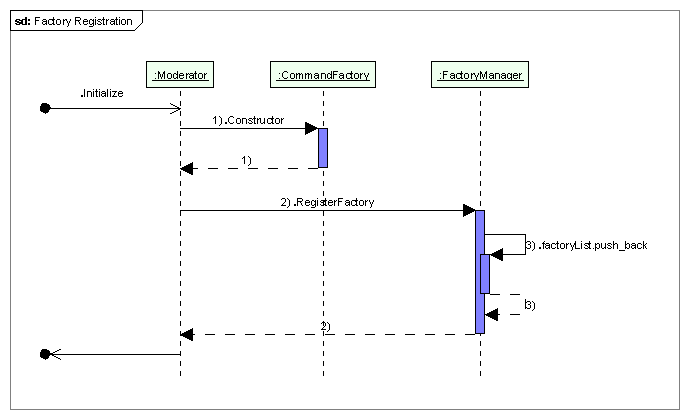
\includegraphics[345,210]{Images/FactoryRegistration.png}
% \caption{Registering a Factory}
% \label{figure:FactoryRegistration}
% \end{center}
% \end{figure}
% 
% The factory registration process, shown in Figure~\ref{figure:FactoryRegistration}, is
% straightforward.  The process starts with the Moderator.  The Moderator retrieves a pointer to the
% Factory that needs to be registered, either through object creation during initialization, or
% through the user factory registration process\footnote{The user registration process will be
% implemented in a future build.}.  In the illustrated example, the factory created is the
% CommandFactory.  The Moderator creates the CommandFactory during initialization.  It takes the
% pointer to the created factory, and passes it to the Factory Manager using the RegisterFactory
% method.  The Factory Manager receives the pointer, and adds it to the list of managed factories by
% pushing it onto the std::vector of factories.  This completes the Factory registration process.
% 
% \subsection{\label{section:CreatingObjectsWithFactMan}Object Creation through the Factory Manager}
% 
% The Factory Manager routes requests for user objects to specific factories, and passes the created
% objects back to the calling routine.  The procedure followed for this process is shown in
% Figure~\ref{figure:FactoryCreation}.
% 
% \begin{figure}[htb]
% \begin{center}
% 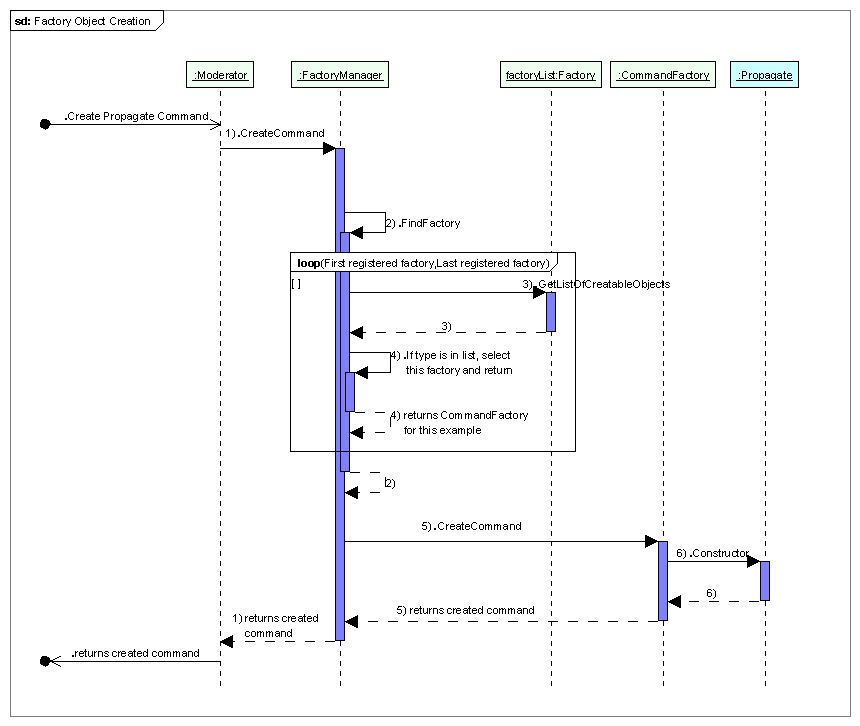
\includegraphics[430,363]{Images/FactoryObjectCreation.png}
% \caption{Creating an Object Using the Factory Subsystem}
% \label{figure:FactoryCreation}
% \end{center}
% \end{figure}
% 
% The process starts when the Moderator receives a message requesting a user object of a given type,
% optionally with a given name.  In the example shown in the figure, the request was for a Propagate
% command.  The Moderator receives the request through a call to the CreateCommand() method,
%typically
% with the syntax ``CreateCommand(``Propagate'',``'')'' for commands.  Named objects receive the
% desired name as the second parameter in this call.  The Moderator calls the Factory Manager's
% CreateCommand() method with the same parameters.
% 
% The Factory Manager calls its FindFactory() method, which locates the factory that can create
% objects of the desired type.  This method works by asking each registered factory for its list of
% creatable types.  FindFactory() checks each list returned from the registered factories until it
% finda a factory that can create the requested object type -- in this example, it searches until it
% finds a factory that can create a ``Propagate'' object.  The CommandFactory creates Propagate
% objects, so that is the factory returned from the FindFactory() method.
% 
% The factory found above is then called and asked for an object of the target type, with the name
% passed in the second parameter of the call.  The factory calls the constructor for that type of
% object -- a Propagate command object in this case -- and returns the pointer to the new object.
% This pointer is returned from the Factory Manager to the Moderator\footnote{The Moderator may
% perform other actions as well -- for instance, named objects may be passed to the Configuration
% Manager, and commands may be inserted into the Mission Control Sequence.  The Moderator actions
% taken are discussed in Chapter~\ref{chapter:TopLevel}; this discussion is only intended to provide
%a
% view into the process followed by the Factory Manager.}, and from the Moderator to the function
%that
% made the call that initiated this sequence, completing the requested task.
% 
% \section{\label{section:ConfigManOverview}The Configuration Manager}
% 
% Objects created by the Factory subsystem are stored in one of two places.  Commands are stored in
% the Mission Control Sequence.  The other objects created in the factories are stored in the
% configuration, a vector of pointers to GmatBase derivatives that is accessed by object name.  Most
% of these objects are stored directly in this vector.  Some objects are stored as objects contained
% in an object in the configuration.  An example of the latter form of object management is a
%planet,
% stored in a solar system object, which is then managed by the Configuration Manager.
% 
% \subsection{\label{section:ConfigManAttributes}Attributes and Methods of the Configuration
%Manager}
% 
% \begin{figure}[htb]
% \begin{center}
% 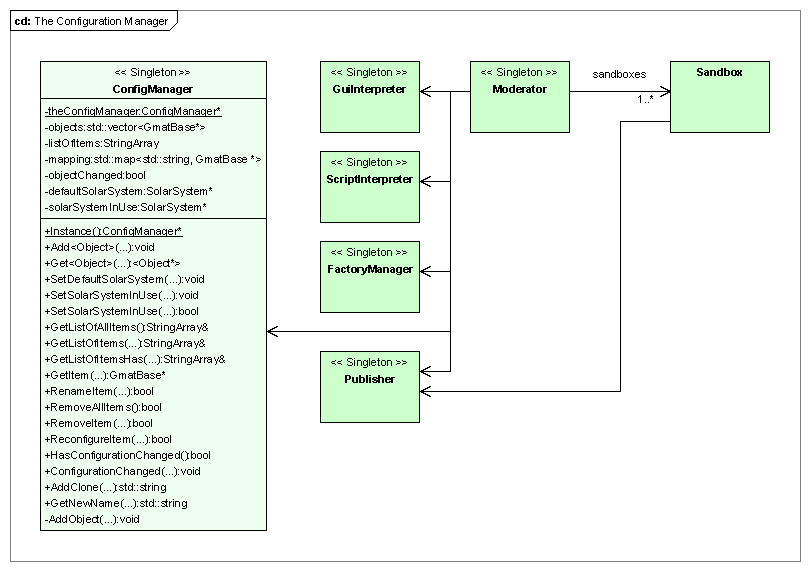
\includegraphics[405,286]{Images/TheConfigurationManager.png}
% \caption{The Configuration Manager in its Environment}
% \label{figure:ConfigManClassDiagram}
% \end{center}
% \end{figure}
% 
% The structure of the Configuration Manager is shown in Figure~\ref{figure:ConfigManClassDiagram}.
% The attributes and methods shown in this figure are described below.
% 
% \subparagraph{\textit{Class Attributes}}
% 
% The configuration is the core element managed by the Configuration Manager.  It is stored in a
% vector of GmatBase pointers named objects.  A related component, the mapping object map, keeps
%track
% of the names of the configured objects and the associated object pointers so that retrieval by
%name
% can be managed easily.  All of the Configuration Manager attributes are listed here:
% 
% \begin{itemize}
% \item \textbf{static ConfigManager* theConfigManager}: The Configuration Manager singleton.
% \item \textbf{std::vector<GmatBase*> objects}: The configuration.
% \item \textbf{StringArray listOfItems}: Array used to store lists of named items that are returned
% from some of the Configuration Manager interfaces.
% \item \textbf{std::map<std::string, GmatBase*> mapping}:  A mapping of object names to the
%pointers
% to the configured objects.  This construct simplifies retrieval of objects from the configuration.
% \item \textbf{bool objectChanged}: A flag indicating if an object in the configuration has
%changed.
% \item \textbf{SolarSystem *defaultSolarSystem}: The default solar system object.
% \item \textbf{SolarSystem *solarSystemInUse}: The current solar system selected for editing or for
%a
% run.
% \end{itemize}
% 
% \subparagraph{\textit{Methods}}
% 
% The Configuration Manager provides interfaces designed to manage insertion, access, and deletion
%of
% objects in the configuration, along with utility method that facilitate object renaming and
%queries
% into the associations between objects.
% 
% Like the Moderator and Factory Manager, the Configuration Manager has methods to add and retrieve
% objects of specific types.  These methods are listed here using the generic ``<Object>'' notation,
% rather than listing all of the specific methods.  Interested users should refer to the source code
% or Doxygen generated documentation to see the specific methods incorporated in the Configuration
% Manager.
% 
% The methods supported by the Configuration Manager are listed here:
% 
% \begin{itemize}
% \item \textbf{static ConfigManager* Instance()}:  Method used to access the Configuration Manager
% singleton.
% \item \textbf{void Add<Object>(<Object*> obj)}: Method used to add an object of a specific type to
% the configuration.
% \item \textbf{<Object*> Get<Object>(const std::string \&name)}: Used to access an object, of a
% specific type, with a specified name.
% \item \textbf{void SetDefaultSolarSystem(SolarSystem *ss)}: Sets the pointer for the default solar
% system model.
% \item \textbf{void SetSolarSystemInUse(SolarSystem *ss)}: Sets the pointer for the current solar
% system model.  In the current build of GMAT, the default and current solar system models are the
% same; this method is provided to support specification of multiple solar system models in a future
% build.
% \item \textbf{bool SetSolarSystemInUse(const std::string \&name)}: Sets the current solar system
%by
% specifying the name of a configured solar system model by name.  This method is provided to
%support
% specification of multiple solar system models in a future build.
% \item \textbf{StringArray\& GetListOfAllItems()}: Retrieves a list of the names of all of the
% objects in the configuration.
% \item \textbf{StringArray\& GetListOfItems(Gmat::ObjectType itemType)}: Retrieves a list of the
% names of all of the objects in the configuration of a specific type.
% \item \textbf{StringArray\& GetListOfItemsHas(Gmat::ObjectType type, const std::string \&name,
%bool
% includeSysParam = true)}:  Searches the configuration to determine if a specific named object is
% used by other configured objects.  For each such usage, the name of the object that uses the named
% object is added to the returned list.
% \item \textbf{GmatBase* GetItem(const std::string \&name)}:  Retrieves an object from the
% configuration and returns its pointer.
% \item \textbf{bool RenameItem(Gmat::ObjectType itemType, const std::string \&oldName, const \\
% std::string \&newName)}:  Renames an object in the configuration.
% \item \textbf{bool RemoveAllItems()}: Clears the configuration so that a new mission can be
% constructed without preserving previously created objects.
% \item \textbf{bool RemoveItem(Gmat::ObjectType type, const std::string \&name)}:  Removes a single
% object from the configuration.
% \item \textbf{bool ReconfigureItem(GmatBase *newobj, const std::string \&name)}:  Resets the
%pointer
% to a configured object with a new object pointer.
% \item \textbf{bool HasConfigurationChanged()}:  Reports the value of the objectChanged flag.
% \item \textbf{void ConfigurationChanged(bool tf)}:  Sets the value of the objectChanged flag.
% \item \textbf{std::string AddClone(const std::string \&name)}:  Clones an object and adds the
%cloned
% object to the configuration.
% \item \textbf{std::string GetNewName(const std::string \&name, Integer startCount)}:  Creates a
%new,
% unique object name based on a current name.
% \item \textbf{void AddObject(GmatBase* obj)}: Adds an object to the configuration and the object
% map.  This private method if the method that actually performs the insertion into the
%configuration
% vector.
% \end{itemize}
% 
% \section{\label{section:SandboxOverview}The Sandbox}
% 
% GMAT's model contains descriptions of the components that are used during a run and the sequence
%of
% events that needs to be executed in order to perform the run.  These pieces are assembled and
% executed in the GMAT Sandbox.  The Sandbox is created by the Moderator.  It is passed the solar
% system configuration for the run, the spacecraft and related objects used in the run, and the
% Mission Control Sequence that fires for the run.
% 
% \begin{figure}[htb]
% \begin{center}
% 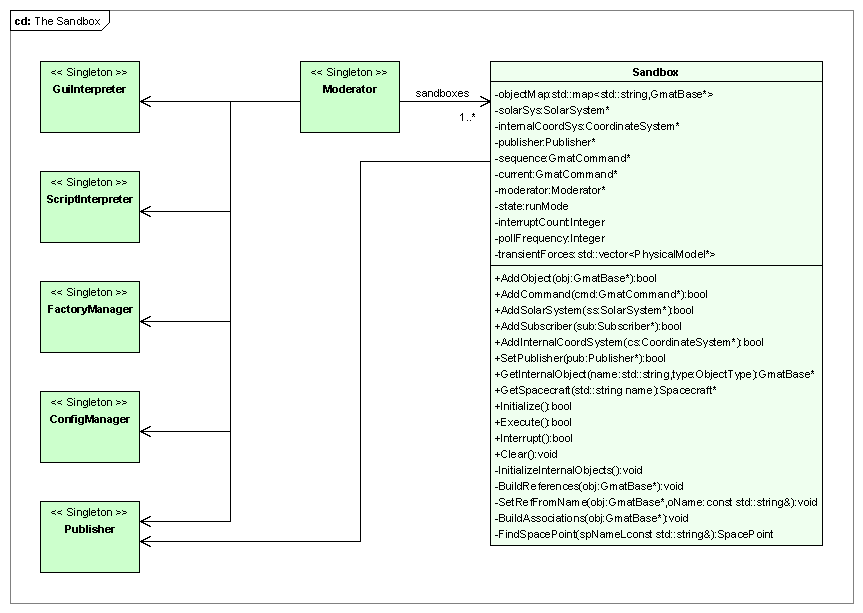
\includegraphics[432,307]{Images/TheSandbox.png}
% \caption{The Sandbox in its Environment}
% \label{figure:SandboxClassDiagram}
% \end{center}
% \end{figure}
% 
% The Sandbox manages objects internally through base class pointers, making its interfaces and
% internal data structures relatively straightforward.  The structure of the Sandbox is shown in
% Figure~\ref{figure:SandboxClassDiagram} and described in the following paragraphs.
% 
% \subsection{\label{section:SandboxAttributes}Attributes and Methods of the Sandbox Class}
% 
% The Sandbox contains the data members necessary for maintaining a local copy of the model and
% running a mission using the model.  It includes members used to communicate with the Moderator and
% Publisher, so that the processes outside of the Sandbox can control the mission run and receive
%data
% resulting from that run.  The class attributes that enable this functionality are listed here.
% 
% \subparagraph{\textit{Class Attributes}}
% 
% \begin{itemize}
% \item \textbf{std::map<std::string, GmatBase *> objectMap}: The local object map in the Sandbox,
% filled by cloning objects from the configuration.
% \item \textbf{SolarSystem *solarSys}: The solar system model used when running the Mission Control
% Sequence in the Sandbox.
% \item \textbf{CoordinateSystem *internalCoordSys}: The reference coordinate system used when
% performing conversions.
% \item \textbf{Publisher *publisher}: The GMAT publisher.
% \item \textbf{GmatCommand *sequence}: The Mission Control Sequence.
% \item \textbf{GmatCommand *current}: The current command in the Mission Control Sequence.  This
% pointer is used to traverse the linked list during a run.
% \item \textbf{Moderator *moderator}: The GMAT Moderator.
% \item \textbf{runMode state}: The current state of the Sandbox.  The Sandbox state model is
% described in Section~\ref{section:StatesintheSandbox}.
% \item \textbf{Integer interruptCount}: A counter used to track polling between the Sandbox and the
% Moderator, so that user interrupts can be processed during a run.
% \item \textbf{Integer pollFrequency}: The frequency used by the Sandbox to poll the Moderator.
% \item \textbf{std::vector<PhysicalModel *> transientForces}: A vector of forces that can be turned
% on or off in a force model during integration.
% \end{itemize}
% 
% \subparagraph{\textit{Public Methods}}
% 
% The Moderator controls model loading and the state of the Sandbox through the following public
% methods.
% 
% \begin{itemize}
% \item \textbf{bool AddObject(GmatBase *obj)}: Adds objects to the local object map.
% \item \textbf{bool AddCommand(GmatCommand *cmd)}: Sets the Mission Control Sequence.
% \item \textbf{bool AddSolarSystem(SolarSystem *ss)}: Sets the solar system model used in a run.
% \item \textbf{bool AddSubscriber(Subscriber *sub)}: Sets subscribers for the run.  This method
% registers the subscriber with the Publisher, and places the Subscriber in the local object map.
% \item \textbf{bool SetInternalCoordSystem(CoordinateSystem *ss)}: Sets the internal coordinate
% system used by the Sandbox.
% \item \textbf{bool SetPublisher(Publisher *pub = NULL)}: Sets the Publisher pointer for the
%Sandbox.
% \item \textbf{GmatBase* GetInternalObject(std::string name, Gmat::ObjectType type = \\
% Gmat::UNKNOWN\_OBJECT)}: Retrieves an object from the local object map by name.
% \item \textbf{bool Initialize()}: Initializes the Sandbox.
% \item \textbf{bool Execute()}: Runs the Mission Control Sequence.
% \item \textbf{bool Interrupt()}: Polls the Moderator to determine is a user action requires a
%state
% change in the Sandbox.
% \item \textbf{void Clear()}: Deletes clones from the local object map, clears the Sandbox's
%Mission
% Control Sequence and transient force vectors, and sets the Sandbox state to IDLE.
% \end{itemize}
% 
% \subparagraph{\textit{Private Methods}}
% 
% The Sandbox uses the following methods internally to initialize and run a mission.
% 
% \begin{itemize}
% \item \textbf{void InitializeInternalObjects()}: Sets up object references in the Sandbox's
%internal
% coordinate system and solar system.
% \item \textbf{void BuildReferences(GmatBase *obj)}: Helper method that sets all internal
%references
% for the input object.
% \item \textbf{void SetRefFromName(GmatBase *obj, const std::string \&oName)}: Finds a named object
% and sets its reference on the input object.
% \item \textbf{void BuildAssociations(GmatBase *obj)}: Finds referenced objects that need to be
% associated with the input object through cloning, creates the clones, and hands the cloned object
%to
% the owner.
% \item \textbf{SpacePoint* FindSpacePoint(const std::string \&spName)}: Finds a SpacePoint by name
% and returns it.
% \end{itemize}
% 
% \subsection{\label{section:StatesintheSandbox}State in the Sandbox}
% 
% The Sandbox maintains state information in the ``state'' member variable.  The state member is set
% to an internal enumerated value, set to one of the values of the runState enumeration designed to
% track the status of the model in the Sandbox.  This enumeration is listed in
% Table~\ref{table:SandboxRunMode}.
% 
% \begin{table}[H]
% \begin{center}
% \caption{\label{table:SandboxRunMode}Values for the Sandbox runState Enumeration}
% \setlength\extrarowheight{2pt}
% \begin{tabular}{|p{1.7in}|p{4in}|}
% \hline
% Identifier & Description \\
% \hline
% \hline
% IDLE & The Sandbox is waiting for the Moderator to prompt for a new run.  Initialized to 7001. \\
% INITIALIZED & The Sandbox has successfully initialized the local object map and the Mission
%Control
% Sequence.\\
% RUNNING & A Mission Control Sequence is executing.\\
% PAUSED & The Moderator has paused a Mission Control Sequence run.  The Sandbox is ready to resume
% the run when the Moderator triggers the run. \\
% STOPPED & The Mission Control Sequence was interrupted by the Moderator, and will not be
%resumed.\\
% RESET & The Sandbox is being reset for a new run.  This state is not used in the current
% implementation.\\
% \hline
% \end{tabular}
% \end{center}
% \end{table}
% 
% Figure~\ref{figure:SandboxStateDiagram} shows the state transitions that the Sandbox uses over the
% course of a typical session with GMAT.  The Sandbox state is initialized to the IDLE state when
%the
% Sandbox is created by the Moderator.  It remains in this state until the sandbox is needed for a
% mission run.  The sequence of events resulting in a mission run were shown in
% Figure~\ref{figure:RunningBasicScript} of Chapter~\ref{chapter:TopLevel}.  These events cause the
% sandbox transitions shown in the figure presented here.
% 
% \begin{figure}[htb]
% \begin{center}
% 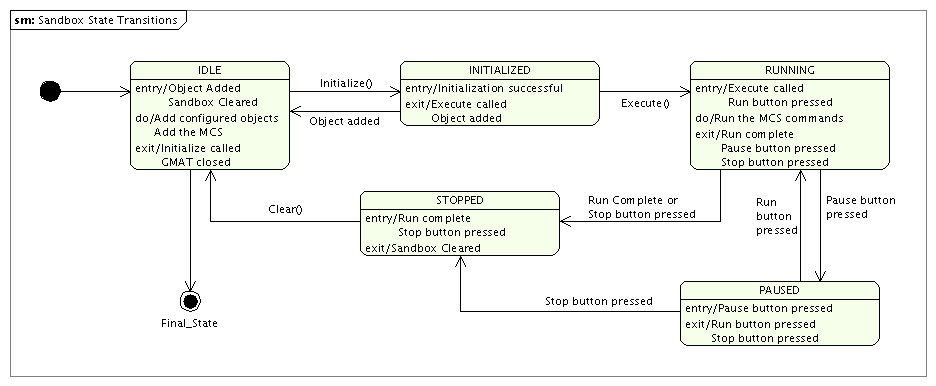
\includegraphics[455,188]{Images/SandboxStateTransitions.png}
% \caption{State Transitions in the Sandbox}
% \label{figure:SandboxStateDiagram}
% \end{center}
% \end{figure}
% 
% When the Moderator recieves a message to run a mission, it passes the configured objects and the
% Mission Control Sequence into the sandbox.  The sandbox adds the objects to the local object map
%and
% sets the sequence pointer in response to these actions, remaining in the IDLE state.  The
%Moderator
% triggers the transition from the IDLE state to the INITIALIZED state by calling the Initialize()
% method.  This method queries each object in the sandbox for referenced objects, and sets the local
% pointers to those references on each object.  If all of the local references were set
%successfully,
% the sandbox transitions to the INITIALIZED state.
% 
% \label{section:SandboxLateBinding}This binding of the reference object pointers happens inside of
% the sandbox so that the reference pointers can be set to the local clones in the sandbox.  This
%late
% binding feature is part of the GMAT design, and is incorporated in that design so that the system
% can support multiple sandboxes, and so that the system can distribute processing to multiple
% processors in future builds.
% 
% When the sandbox completes initialization, all of the components in the sandbox have their local
% references set, and the system is ready to run a Mission Control Sequence.  There are two possible
% transitions from the INITIALIZED state.  The Moderator can add additional elements to the sandbox.
% If any additional element is added, the sandbox returns to the IDLE state, indicating that object
% references have had the opportunity to be set for all of the objects in the sandbox.
% 
% The more interesting transition happens in response to a call of the Execute method from the
% Moderator.  When the Moderator calls the Execute() method, the sandbox transitions into the
%RUNNING
% state.  The sandbox starts executing the commands in the Mission Control Sequence, and runs these
% commands until either the mission runs to completion, an error occurs in the run, or the user
% interrupts processing by pressing the stop or pause button on the GUI.
% 
% If the user presses the pause button on the GUI, the sandbox transitions into the PAUSED state,
% maintaining the information required to resume the run.  From the PAUSED state, the user can
%either
% terminate the run by pressing the stop button or resume the run by pressing the run button on the
% GUI.  Pressing the stop button transitions the sandbox into the STOPPED state.  Pressing the run
% button causes a transition back into the RUNNING state, and execution of the Mission Control
% Sequence resumes from the point where the pause message was received by the sandbox.
% 
% Once the run has terminated, either by running to completion, running to an error in the sequence,
% or through a user interrupt generated by the stop button, the sandbox enters the STOPPED state. 
%In
% the STOPPED state, all of the objects in the sandbox remain in their post execution state.  This
% feature allows some limited user access to the post-run data; for example, the user can retrieve
% data at the end of execution of each command using the Command Summary panel in the GUI.  The
% sandbox's local objects remain in this post-run state until the sandbox is cleared by the
%Moderator.
% 
% The Moderator clears a sandbox by calling the Clear method.  The Clear() method destroys all of
%the
% objects in the sandbox's local object map, releases the Mission Control Sequence pointer, and
% transitions the sandbox into the IDLE state, closing the state transition loop shown
% in Figure~\ref{figure:SandboxStateDiagram}.
% 
% When GMAT closes down, the Moderator destroys the sandboxes in the system.  This last transition
% moves each sandbox from the IDLE state to the final state shown in the figure.
% 
% \subsection{\label{section:SandboxInterruptPolling}Interrupt Polling in the Sandbox}
% 
% One feature of the sandbox state transitions described above is the interaction between the
%Sandbox
% and the rest of GMAT performed to process user interrupts.  In the current implementation, the
% sandbox takes over execution when a Mission Control Sequence is running.  Each command is executed
% in order, and the sandbox moves from one command to the next in the list of commands.  Commands
%are
% executed by calling a command specific Execute() method.
% 
% Between each call to these Execute() methods, the sandbox is given the opportunity to query the
% Moderator for user interrupts.  The sandbox performs this operation periodically.  The Moderator,
% in turn, queries the GuiInterpreter for user interrupts, and the GuiInterpreter queries the GUI.
% The GUI processes any pending messages, and, if the user has presses the pause or stop button,
% sends the interrupt through the GuiInterpreter to the Moderator.  The sandbox retrieves this
% interrupt from the Moderator, and triggers the corresponding state transition, as described above.
% 
% \section{\label{section:PublisherOverview}The Publisher}
% 
% During a run users can monitor the progress through the Mission Control Sequence by watching the
% trajectory evolve in OpenGL windows, parameters change value in plot windows, and on some systems
%by
% watching data flow into output files.  GMAT uses a publish and subscribe system to drive all of
% these pipelines from the Sandbox to user viewable data sources.  The engine drives the data
%transfer
% from the Sandbox to the output objects using a singleton called the Publisher.
% 
% Data generated during a run is sent from the Sandbox containing the run to the Publisher
%singleton.
% The Publisher receives the Sandbox data, and sends the data to each Subscriber registered with the
% Publisher.  Subscribers, described in Chapter~\ref{chapter:Factories}, contain common interfaces
% that the Publisher uses to push data received from the Sandbox to the Subscribers.  Note that a
%key
% element of the publish and subscribe algorithm implemented in GMAT is that data flows in one
% direction: data is generated in the Sandbox, passed to the Publisher, and then passed from the
% Publisher to the Subscribers.
% 
% The Publisher class attributes and interfaces that enable this functionality are listed here.
% 
% \subsection{\label{section:PublisherAttributes}Attributes and Methods of the Publisher}
% 
% \begin{figure}[htb]
% \begin{center}
% 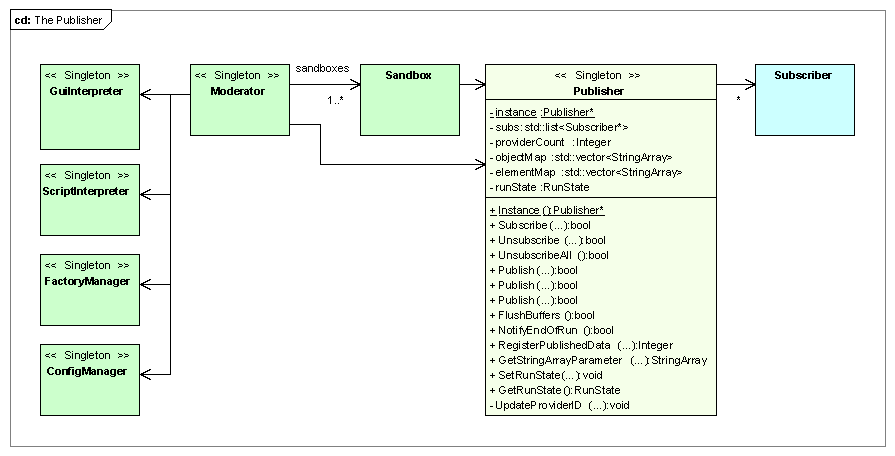
\includegraphics[445,227]{Images/ThePublisher.png}
% \caption{The Publisher in its Environment}
% \label{figure:PublisherClassDiagram}
% \end{center}
% \end{figure}
% 
% Figure~\ref{figure:PublisherClassDiagram} shows the attributes and methods incorporated in the
% Publisher.
% 
% \subparagraph{\textit{Class Attributes}}
% 
% The Publisher maintains a collection of Subscribers that are registered to receive data and
% information about the current state of GMAT in order to manage the data transfer tasks during a
%run.
%  The following attribute list is built into the Publisher to perform this maintenance:
% 
% \begin{itemize}
% \item \textbf{static Publisher *instance}:  The Publisher singleton.
% \item \textbf{std::list<Subscriber*> subs}:  The current list of Subscribers supported by the
% Publisher.
% \item \textbf{Integer providerCount}:  The number of registered data providers.
% \item \textbf{Integer currentProvider}:  The current data provider sending data to the publisher.
% \item \textbf{std::vector<StringArray> objectMap}:  List of the names of objects providing data.
% \item \textbf{std::vector<StringArray> elementMap}:  List of the names of the data elements
%provided
% to the Publisher.
% \item \textbf{Gmat::RunState runState}:  The current run state for GMAT.  The Publisher tracks the
% current run state so that Subscribers can act differently based on the current state of the
%system.
% \end{itemize}
% 
% \noindent Note that the data structures in the Publisher currently support only one set of data
% structures, mapping to a single Mission Control Sequence.  When GMAT is extended to support
%multiple
% Sandboxes, these data structures may be changed to add support for multiple Sandboxes.
% 
% \subparagraph{\textit{Methods}}
% 
% Interfaces into the Publisher are provided through the following methods:
% 
% \begin{itemize}
% \item \textbf{static Publisher* Instance()}:  Method used to access the Publisher singleton.
% \item \textbf{bool Subscribe(Subscriber *s)}:  The registration interface for the Subscribers.
% \item \textbf{bool Unsubscribe(Subscriber *s)}:  The method used to remove a Subscriber from the
% list of data receivers.
% \item \textbf{bool UnsubscribeAll()}:  Removes all Subscribers from the list of data receivers
% \item \textbf{bool Publish(Integer id, Real *data, Integer count)}:  Passes an array of Real data
% from the data source identified by id number to the Subscribers.
% \item \textbf{bool Publish(Integer id, char *data, Integer count = 0)}:  Passes an array of
% character data from the data source identified by id number to the Subscribers.
% \item \textbf{bool Publish(Integer id, Integer *data, Integer count)}:  Passes an array of Integer
% data from the data source identified by id number to the Subscribers.
% \item \textbf{bool FlushBuffers()}:  Prompts each registered Subscriber to process all received
%data
% immediately, rather than wait for an input buffer to be filled.
% \item \textbf{bool NotifyEndOfRun()}:  Tells each registered Subscriber that the Mission Control
% Sequence has finished running.
% \item \textbf{Integer RegisterPublishedData(const StringArray\& owners, const StringArray\&
% elements)}:  Registers data providers with the Publisher.  The returned value is the id for the
% registered data provider.
% \item \textbf{const StringArray\& GetStringArrayParameter(const std::string\& type)}:  Accesses
%the
% strings in the objectMap and elementMap members.
% \item \textbf{void SetRunState(const Gmat::RunState state)}:  Sets the run state for the
%Publisher.
% \item \textbf{inline Gmat::RunState GetRunState()}:  Accesses the current run state.
% \item \textbf{void UpdateProviderID(Integer newId)}:  Resets the ids for the Subscribers.
% \end{itemize}
% 
% \subsection{\label{section:PublisherStates}State Transitions in the Publisher}
% 
% \begin{figure}[htb]
% \begin{center}
% 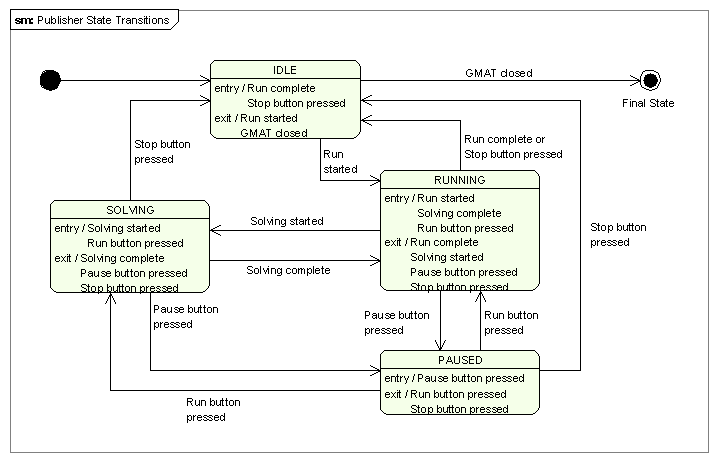
\includegraphics[359,231]{Images/PublisherStateTransitions.png}
% \caption{State Transitions in the Publisher}
% \label{figure:PublisherStateDiagram}
% \end{center}
% \end{figure}
% 
% Subscribers have the option to act differently based on the current status of the run -- for
% example, the OpenGL Subscriber can be set to show all of the published data, or only data
%published
% when the Mission Control Sequence is not running iterations through a Solver.  The Subscribers
%track
% this information through state data maintained by the Publisher.  The states tracked by the
% Publisher are shown in Figure~\ref{figure:PublisherStateDiagram}.
% 
% The Publisher starts in the IDLE state, and returns to this state when a Mission Control Sequence
% stops running.  The Publisher moves from the IDLE state to the RUNNING state when a user starts
% execution of a Mission Control Sequence.
% 
% The RUNNING state is the nominal state for the Publisher when a Mission Control Sequence is being
% executed.  The Publisher moves into the SOLVING state whenever a Solver loop is searching for a
% solution -- that is, whenever a Target command is targeting, and Optimize command is optimizing,
%or
% an Iterate command is iterating over a set of variables.  The Publisher remains in the SOLVING
%state
% until the Solver finds a solution; at that point the Publisher returns to the RUNNING state.
% 
% Users can interrupt the Mission Control Sequence by pressing either the Pause or Stop button on
%the
% GUI.  When the Pause button is pressed, the Publisher transitions into the PAUSED state.  If the
% mission resumes (i.e. if the user pressed the Run button for the paused mission), the Publisher
% returns to its previous state -- either RUNNING or SOLVING, based on the state of the Mission
% Control Sequence.  If the user presses the Stop button, the Publisher moves into the IDLE state.


\chapter{\label{chapter:Moderator}The Moderator}

The entry point into GMAT's engine is the Moderator.  The Moderator controls program flow, creating
components through the factory manager that are then managed in the configuration manager, and
then using these components to model missions in a sandbox.  The Moderator creates the engine
components, manages those components when necessary, and controls the processes in GMAT's engine. 
It initializes the Sandbox prior to a run, and launches the run in the Sandbox.  In other words, the
Moderator is the central control element of GMAT, acting as the interface between users and the
internal elements of the system, and facilitating communications between those internal elements.

The engine contains one component, the Publisher, that does not interact with the Moderator beyond
initialization.  The Publisher, described in Chapter~\ref{chapter:Publisher}, is the communications
interface between the Sandbox objects and the Subscriber objects that present data to users.  The
following sections discuss interactions between engine components and the Moderator.With the
exception of initialization, these interactions exclude the Publisher.

This chapter explains how the Moderator accomplishes its tasks.

\section{Moderator Design Principles}

Figure~\ref{figure:GMATStackDiagram} shows a high level view into GMAT's architecture.  That figure
contains arrows showing all of the allowed communications paths in the engine.
Figure~\ref{figure:ModeratorInteractions} shows the portion of that diagram that corresponds to the
Moderator's role in GMAT.  The Moderator handles all communications between the Interpreters and
the engine, and between the components of the engine used to set up and run a mission.

\begin{figure}[htb]
\begin{center}
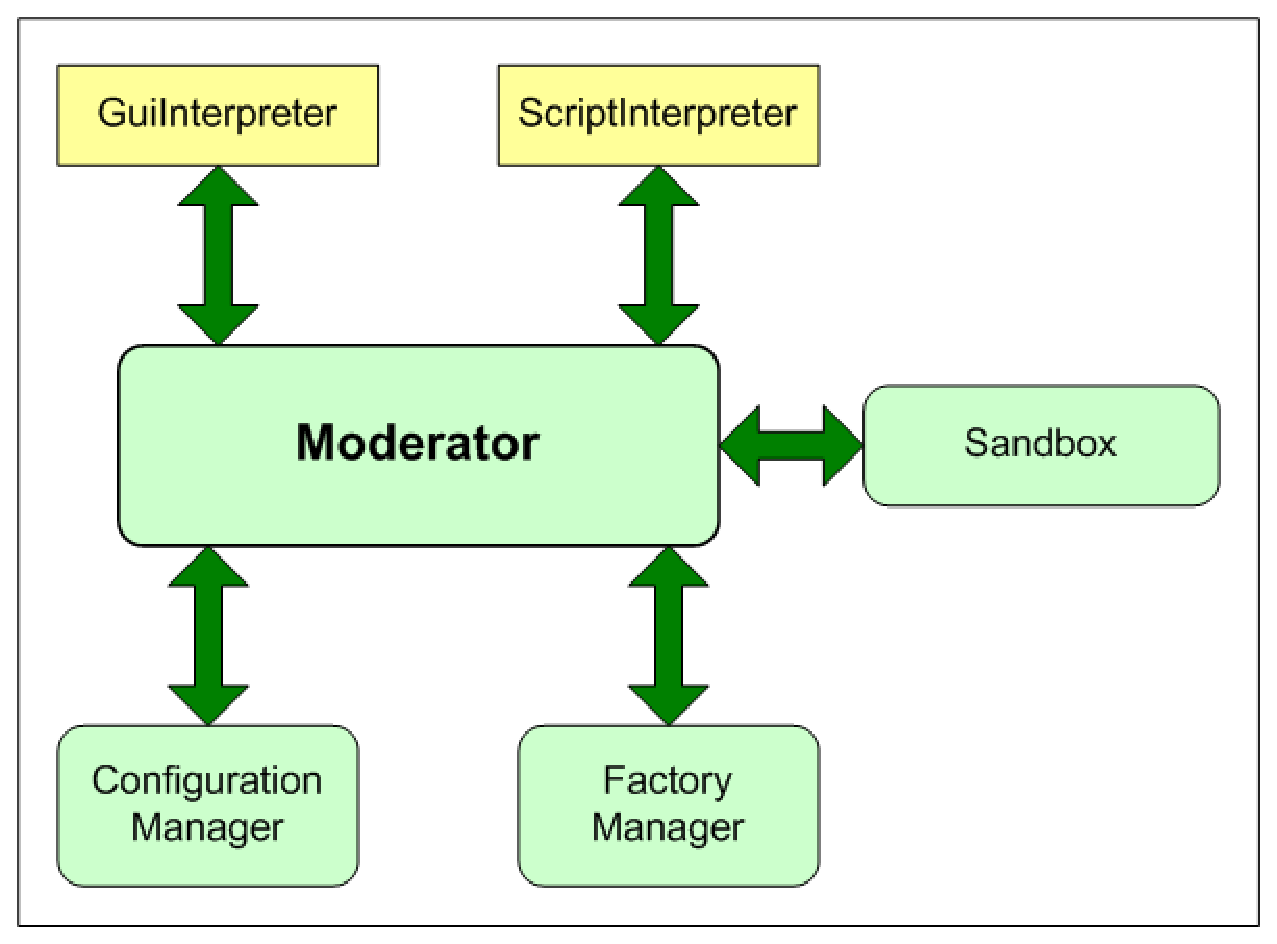
\includegraphics[scale=0.5]{Images/ModeratorInteractions.eps}
\caption{Program Flow and the Moderator}
\label{figure:ModeratorInteractions}
\end{center}
\end{figure}

While the arrows in this figure show the information flow through the Moderator, they do not state
explicitly what data or objects move along these paths.  The Moderator is the manager for all of
the tasks accomplished in the engine.

The Moderator design is built around two design patterns: the Singleton pattern and the Mediator
pattern.  The Mediator pattern is discussed in Section~\ref{section:ModeratorMediator}.  The
Moderator consolidates the management actions needed for GMAT into a central location.  It is a
singleton to ensure that this consolidation happens at only one place for the GMAT executable.  Each
instance of GMAT running in memory has exactly one Moderator managing the GMAT engine.

There are seven key actions that the Moderator is responsible for managing, described in the next
section.

\subsection{Moderator Responsibilities}

The Moderator plays a central role in seven tasks:

\begin{enumerate}
\item \textbf{Engine Initialization:}  The Moderator is responsible for initializing GMAT's engine
when the system starts.
\item \textbf{Object Creation:}  All object creation requests made by users are passed, through an
Interpreter, to the Moderator.  The Moderator starts this process by passing creation requests to
the factory subsystem, and completes it by sending the created objects to their destinations.
\item \textbf{Object Configuration:}  All object configuration requests made by users are passed,
through an Interpreter, to the Moderator.  The Moderator locates the object that needs
configuration, and passes that object to the process that performs the configuration.
\item \textbf{Loading a Script:}  The Moderator works with the Script Interpreter to manage the
creation and configuration process performed when a script file is loaded into the system.
\item \textbf{Running a Mission:}  The Moderator ensures that all of the elements needed to run a
mission are provided to the Sandbox used in the run, and then passes the initialization and run
control into that Sandbox.  The Moderator then monitors the process in the background during the
run, and handles the communications necessary when a user interrupts the run.
\item \textbf{Saving a Mission:}  The Moderator acts as an intermediary between the objects
configured in GMAT and the Interpreters when a mission is saved, locating and serving up the
objects that need to be serialized as needed by the Interpreters.
\item \textbf{User Extension:}  The Moderator provides the interfaces needed to extend GMAT using
user libraries.
\end{enumerate}

Each of these tasks involves communications between components of the engine that, were the
Moderator absent, would be made directly between the engine components.  While that approach may
seem like a more efficient avenue at first, the resulting number and types of communications that
it would necessitate would produce a much more tightly coupled system.  As the number of engine
components increases, the complexity of these component interactions would also increase.  The
Moderator reduces this communications complexity by consolidating the communications into a central
component, using a design pattern called the Mediator pattern.

\subsection{\label{section:ModeratorMediator}The Mediator Pattern Employed in the Moderator}

The Moderator is designed to enforce loose coupling between the elements of GMAT's engine, and to
simplify and standardize the communications between the other elements of the engine. It acts as an
intermediary between user inputs passed in through the script and GUI interpreters, the factory
subsystem used to build objects needed to simulate a mission, the configuration that stores these
configured objects, and the sandboxes that actually run the simulation.  It is built using the
Mediator design pattern, as described in \cite{GoF} and summarized in Appendix
\ref{chapter:Patterns}.  This pattern enforces the following features:

\subparagraph{\textit{Loose Coupling}}  The engine components communicate with each other through
calls into the Moderator.  This feature means that the other engine components do not need to know
how to communicate with each other.  Instead, they make all communications calls to the Moderator,
which is responsible for routing these calls to the appropriate recipients.  In other words, the
Interpreters, Factory Manager, Configuration Manager, and Sandboxes do not know about each other. 
Instead, all of the interactions between these components is made through calls to and from the
Moderator.

\subparagraph{\textit{Maintainability}}  All communications between the Interpreters, Factory
Manager, Configuration Manager, and Sandboxes is performed through the Moderator.  This
consolidation of the information exchange between the components centralizes the location for
communications mishaps, and simplifies the task of correcting these defects as they are detected. 
In addition, the interfaces in the Moderator are designed to be consistent, reducing the number of
different calling protocols that a maintainer needs to learn and understand.

\subsubsection{Implications}

The design of the Moderator as a Mediator produces the following benefits:

\subparagraph{\textit{Decouples Objects}}  Since the internal communications between the components
of the engine pass through the Moderator, the other elements of the engine do not need knowledge
about each other.

\subparagraph{\textit{Simplifies Object Protocols}}  The Moderator simplifies objects by replacing
direct communications between the engine components with communications through a central component.

\subparagraph{\textit{Abstracts Object Communications}}  Since the Moderator stands separate from
the actions taken by the other engine components, work performed by the Moderator has the effect of
reducing the interfaces in the engine components to the minimal set necessary to achieve these
communications.  This feature simplifies those interfaces, and encourages better encapsulation of
the workings of the other components.

\subparagraph{\textit{Centralizes Complexity}}  All of the complexity involved in the communications
between the engine components is captured in the Moderator.  The interactions between the other
engine components is greatly simplified through this design, making the engine easier to understand
and maintain.

\subsubsection{Summary}

To summarize, the design of the Moderator reduces the interaction complexity in GMAT's engine;
communications complexity resides in the Moderator, rather than in the interactions between the
Interpreters and the elements of the engine.  The other objects involved in these communications --
the Script and GUI Interpreters, the Factory Manager, the Configuration Manager, and the Sandboxes
-- are less complex because they only communicate with the Moderator, rather than with each other.
The Moderator is constructed to handle all of the interactions between the interpreters and amongst
the engine components.  You are unlikely to need to make any changes to the Moderator unless you
are adding an unanticipated feature.

\section{Moderator Design}

Figure ~\ref{figure:ModeratorClassDiagram} shows the Moderator, the classes it interacts with, and
some of its internal structures.  The interactions between the Moderator and other elements of
GMAT's engine were presented in Chapter~\ref{chapter:TopLevel}.  The sequence diagrams presented
there describe the interfaces to the Moderator and their usage when constructing and using a model. 
The methods shown in Figure~\ref{figure:ModeratorClassDiagram} present representative examples of
these interfaces in more detail.

\begin{figure}[htb]
\begin{center}
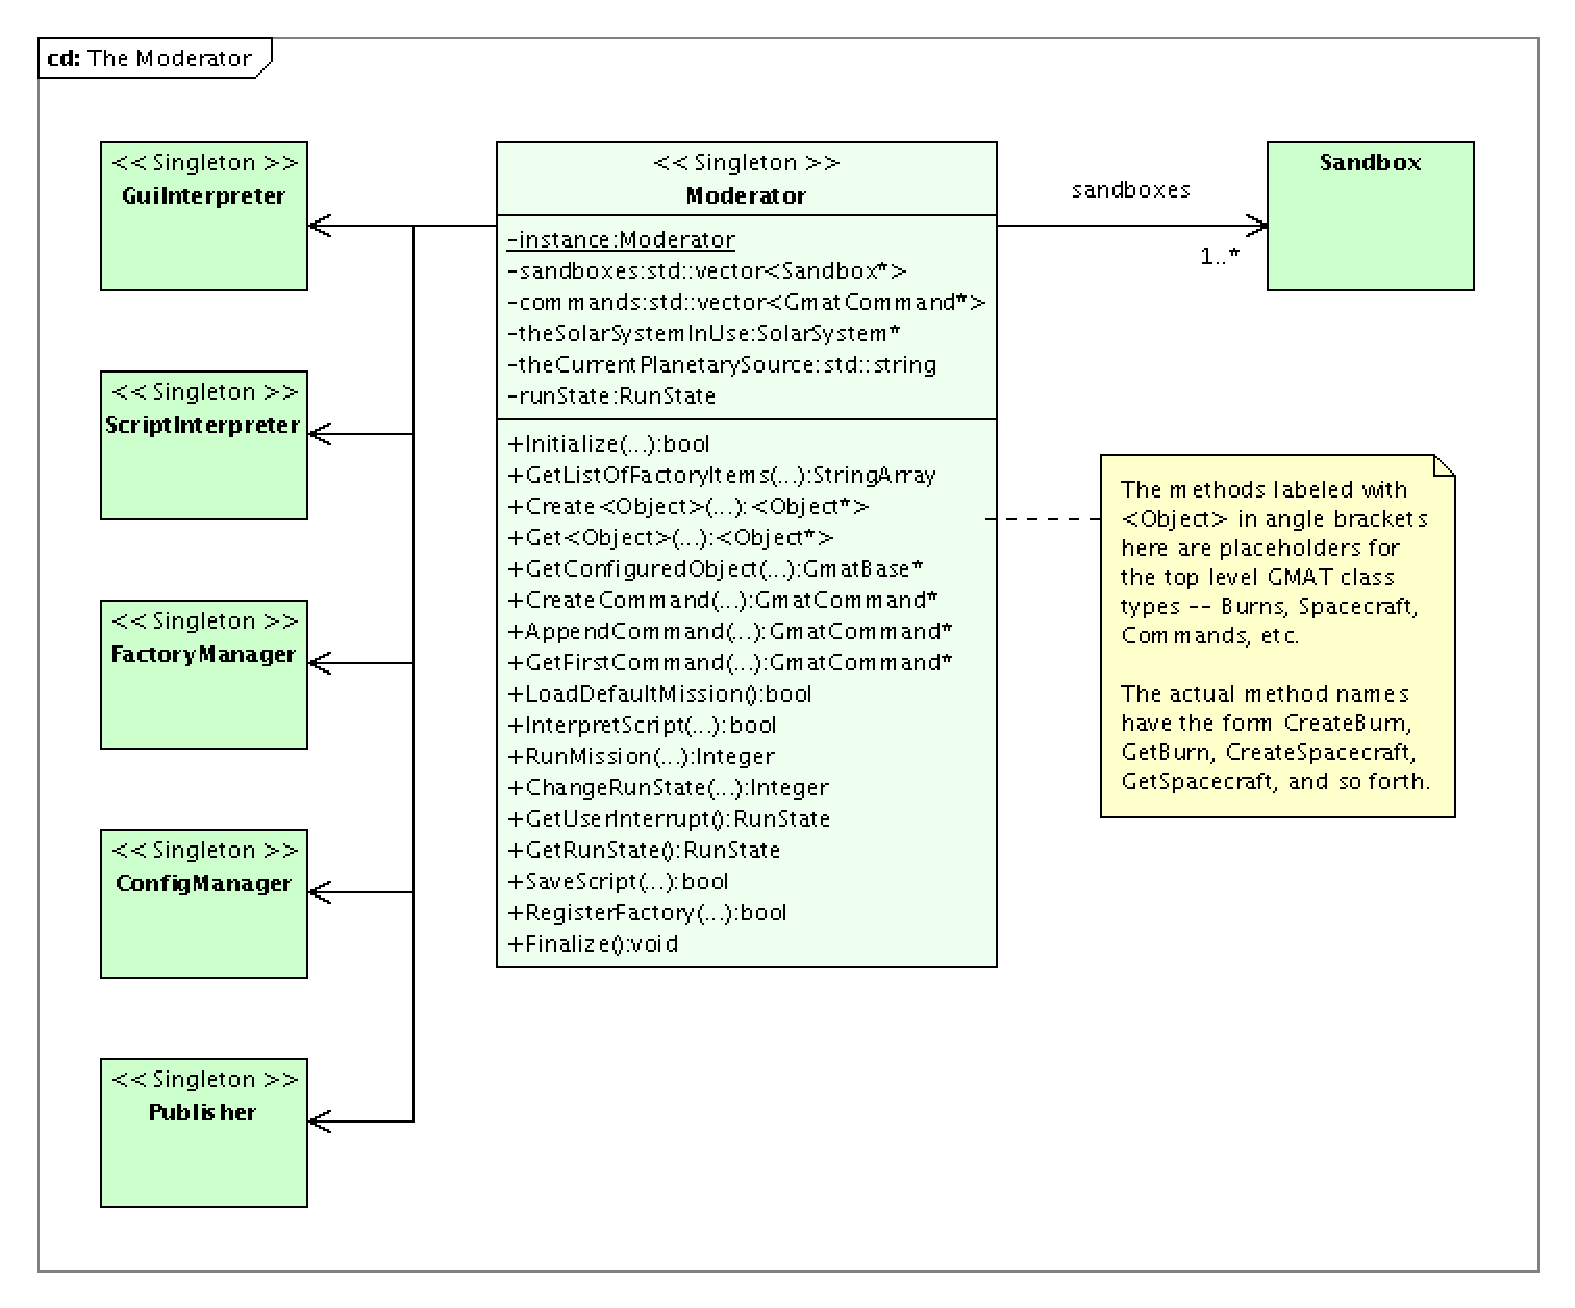
\includegraphics[scale=0.5]{Images/TheModerator.eps}
\caption{The Moderator in its Environment}
\label{figure:ModeratorClassDiagram}
\end{center}
\end{figure}

\subsection{Class Details}

The following paragraphs describe the internal data members used by
the Moderator and a brief discussion of how the methods shown in the figure are used to accomplish
its tasks.  Full details of the Moderator and its members can be found in the Doxygen
documentation, generated by running Doxygen\cite{doxygen} on GMAT's source code.

\subsubsection{Class Attributes}

There are several key data members that the Moderator uses to perform its assigned tasks.  These
members are

\begin{itemize}
\item \textbf{Moderator *instance}:  The \texttt{instance} pointer in the Moderator is the
singleton instance used throughout GMAT.
\item \textbf{std::vector<Sandbox*> sandboxes}:  GMAT's Sandbox class is used to run missions
simulating spacecraft in orbit.  The Sandbox instances are the only key players in the engine which
do not exist as singletons.  Instead, the Sandbox instances are managed by the Moderator using the
\texttt{sandboxes} vector.
\item \textbf{std::vector<GmatCommand*> commands}:  GMAT maintains a 1:1 mapping between the
Sandbox instances and the Mission Control Sequences assigned to each Sandbox.  The Moderator uses
its \texttt{commands} vector to manage the first node of the command sequence linked list for
the Mission Control Sequence of each Sandbox.
\item \textbf{SolarSystem* theSolarSystemInUse}:  GMAT's Solar System model (see
Chapter~\ref{chapter:SolarSystem}) is an aggregated object configured to include all of the bodies,
special points, and other environmental elements necessary for precision spacecraft modeling.  The
Moderator manages the Solar System used in the Sandboxes, and stores the current Solar System in
the \texttt{theSolarSystemInUse} data member.
\item \textbf{std::string theCurrentPlanetarySource}:  This string identifies the source of the
planetary ephemerides used in GMAT's environmental model.
\item \textbf{RunState runState}:  The Moderator keeps track of the current state of the Sandbox
instances in order to facilitate communications about that status between the interpreters and user
interfaces, the Publisher, and the Sandbox instances\footnote{The current implementation uses a
single runState data member.  This data structure will change to a vector when the multiple
Sandbox features of GMAT are enabled.}. The \texttt{runState} member tracks this information for the
Moderator.
\end{itemize}

Each of these class attributes plays a role in the seven tasks managed by the Moderator.
Figure~\ref{figure:ModeratorClassDiagram} also shows several methods used for these tasks.  These
methods and their roles in the Moderator's tasks are described next.

\subsubsection{Initialization and Finalization Methods}

The Moderator is responsible for starting the internal components of GMAT's engine, and for
ensuring that those components exit gracefully when GMAT is closed.  The start up process is
described in some detail in section~\ref{section:GMATStartup}.  Initialization and finalization are
performed through the following two methods:

\begin{itemize}
\item \textbf{bool Initialize(bool isFromGui = false)}:  The \texttt{Initialize} method creates the
core engine components, parses the start up file and sets up the external file pointers for
references contained in that file, and populates the Factory manager with the default factories.
This method should be called before performing any other interactions with the GMAT engine.  The
input parameter, \texttt{isFromGui}, is used to determine if the default mission should be
constructed during initialization.
\item \textbf{void Finalize()}:  The \texttt{Finalize} method is called as GMAT shuts down.  This
method frees memory that was allocated for use by the Moderator, and closes any open files managed
in the Moderator.
\end{itemize}

\subsubsection{Creation and Configuration Methods}

The creation process, described in Section~\ref{section:ObjectCreation} for configured objects and
in Section~\ref{section:CommandCreation} for commands, allocates objects and stores them in GMAT's
configuration database or the Mission Control Sequence, respectively.  These objects can then be
accessed by GMAT so that their attributes can be set as needed for the simulation, and, for the
objects in the configuration database, so that they can be copied into a Sandbox prior to a mission
run. The Moderator acts as the intermediary for the creation and object access processes, using
methods tailored to these actions.

The full set of creation and access methods are best viewed in the Doxygen files.  The following
method descriptions are representative of the full set found there.  The methods listed here use
the Burn classes to illustrate the objects that can be created in GMAT; other types of objects are
created and configured using similar methods.

\begin{itemize}
\item \textbf{StringArray GetListOfFactoryItems(Gmat::ObjectType type)}:  This method returns a
list of all of the creatable types of objects of a given supertype, described by the \texttt{type}
parameter.  For example, if the \texttt{type} parameter is set to the \texttt{BURN} type, the
returned string array contains the entries ``ImpulsiveBurn'' and ``FiniteBurn''.
\item \textbf{Burn* CreateBurn(const std::string \&type, const std::string \&name)}:  Creates a
Burn object of the specified subtype, with the specified name.  The Moderator contains creation
methods for all of GMAT's core types. These methods are all similar in form to the method shown
here; they specify the subtype and name of the requested object, and then return a pointer to the
object if it was created successfully.
\item \textbf{Burn* GetBurn(const std::string \&name)}:  Retrieves the Burn object with the
specified name.  Similar methods exist for all of GMAT's core types.
\item \textbf{GmatBase* GetConfiguredObject(const std::string \&name)}:  Returns a base class
pointer to the configured object of the specified name.
\item \textbf{GmatCommand* CreateCommand(const std::string \&type, const std::string \&name, bool
\&retFlag)}:  Creates a Mission Control Sequence command of the specified type.
\item \textbf{GmatCommand* AppendCommand(const std::string \&type, const std::string \&name, bool
\&retFlag, Integer sandboxNum = 1)}:  Creates a Mission Control Sequence command of the specified
type, and passes it into the Mission Control Sequence associated with the specified Sandbox.
\item \textbf{GmatCommand* GetFirstCommand(Integer sandboxNum = 1)}:  Retrieves the first command
in the Mission Control Sequence associated with the specified Sandbox.  Since the Mission Control
Sequence is a linked list, this method can be used to retrieve the entire Mission Control Sequence.
\end{itemize}

\subsubsection{Reading or Saving a Mission}

The processes followed when loading a mission into GMAT and when saving a mission from GMAT are
managed by the Script Interpreter.

The read process is implemented as a sequence of object creations and configurations in the
Script Interpreter.  The Moderator passes requests for these processes to the Interpreter through
several different methods, including these:

\begin{itemize}
\item \textbf{bool LoadDefaultMission()}:  Clears the current configuration and Mission Control
Sequence from memory, and then creates and configures the default GMAT mission.
\item \textbf{bool InterpretScript(const std::string \&filename, bool readBack = false, const
std::string \&newPath = "")}:  Creates and configures all of the objects in a script file.
\end{itemize}

Each object defining a mission in GMAT includes the ability to serialize itself so that is can be
passed to an external process or written to a file.  The Moderator passes requests for this
serialization to the Script Interpreter for processing.  A representative example of the Moderator
methods used for this process is the \texttt{SaveScript} method:

\begin{itemize}
\item \textbf{bool SaveScript(const std::string \&filename, Gmat::WriteMode mode =
Gmat::SCRIPTING)}:  Builds scripts from the configured objects and commands, and write them to a
file named by the \texttt{filename} parameter.  The writeMode parameter is used to determine the
style of the serialization; it can be set to either the default \texttt{SCRIPTING} style or to a
style, \texttt{MATLAB\_STRUCT}, compatible with MATLAB.
\end{itemize}

\noindent Details of the actual processes followed when reading or writing a script can be found in
Chapter~\ref{chapter:ScriptRW}.

\subsubsection{Methods Used to Run a Mission}

The process followed when GMAT runs a mission is described in
Section~\ref{section:SandboxMCSExecution}.  The process is relatively straightforward: the
configured objects and Mission Control Sequence are loaded into the Sandbox instance, initialized
to establish the connections between those objects, and then run in the Sandbox, as described in
Section~\ref{section:SandboxMCSExecution} and in Chapter~\ref{chapter:Sandbox}.  The Moderator
supports these tasks through the following methods and through similar methods that can be examined
in the Doxygen output.

\begin{itemize}
\item \textbf{Integer RunMission(Integer sandboxNum = 1)}:  Loads objects into the specified
Sandbox, initializes it, and starts the mission run in the Sandbox.
\item \textbf{Integer ChangeRunState(const std::string \&state, Integer sandboxNum = 1)}: 
Method used by the interpreters to update the run state information in the Moderator, so that the
Sandbox can later check the Moderator's run state.
\item \textbf{RunState GetUserInterrupt()}:  Method called to determine if the user has requested a
change in the run state.  This method queries the interpreter for state changes before returning
the run state, so that the interpreter code has an opportunity to update the state based on user
actions.
\item \textbf{RunState GetRunState()}:  Returns the current run state of the Sandbox.
\end{itemize}

The Moderator keeps track of the state of execution in the Sandbox instance so that it can respond
to messages from the interpreters that affect the system, like user commands to pause or terminate
the run.  The discussion in Section~\ref{section:SandboxMCSExecution} presented the program flow
exercised during a mission run.  During the loop through the Mission Control Sequence shown in
Figure~\ref{figure:RunningBasicScript}, the Sandbox polls the Moderator for the execution state.
This polling checks the Moderator's state variable and responds accordingly, as discussed in
Chapter~\ref{chapter:Sandbox}.

\begin{figure}[htb]
\begin{center}
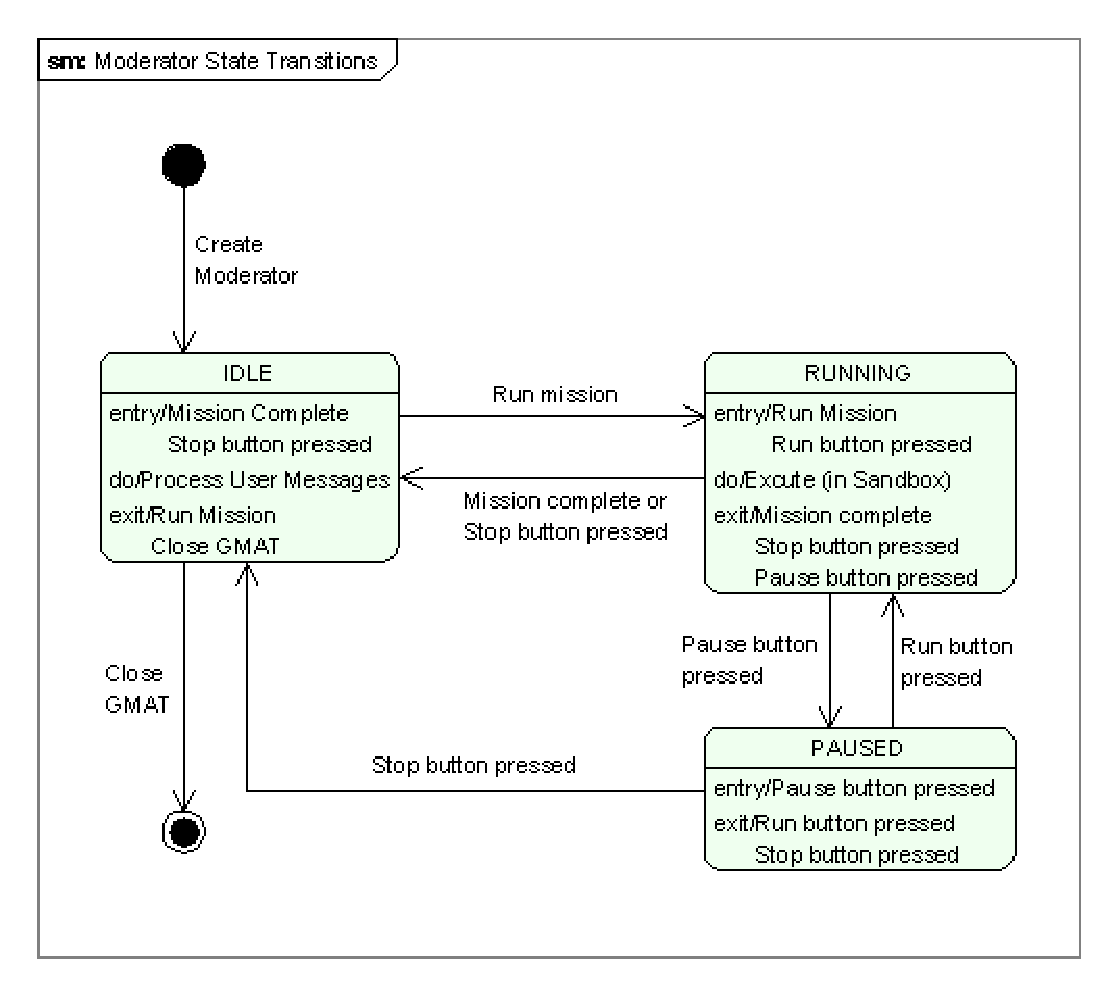
\includegraphics[scale=0.5]{Images/ModeratorStateTransitions.eps}
\caption{State Transitions in the Moderator}
\label{figure:ModeratorStateTransitions}
\end{center}
\end{figure}

\subparagraph{\label{section:ModeratorStates}\textit{State Transitions in the Moderator}}

The Moderator tracks the current state of the system using a parameter named runState, which is set
to a value in the RunState enumeration (see Table~\ref{table:RunStateEnum}) defined in the Gmat
namespace.  The engine states tracked in the Moderator are the IDLE, RUNNING, and PAUSED states.

Figure ~\ref{figure:ModeratorStateTransitions} shows the run state transitions tracked by the
Moderator.  The Moderator is created with the run state set to the IDLE state.  Most of the time,
the Moderator remains in the IDLE state, processing messages from users and managing the internal
components of the GMAT engine\footnote{Many of the activities performed by the Moderator in the IDLE
state are described in Chapter~\ref{chapter:TopLevel}.  Additional Moderator interactions with the
other engine components are described in the appropriate sections of this document.}.

When a user executes a Mission Control Sequence, the Moderator transitions to the RUNNING state.  In
this state, the Moderator performs very limited processing while the control of the system is
managed by the sandbox that is running the mission.  The sandbox polls the Moderator for user
activity at convenient points during the mission run.  This polling allows the Moderator to respond
to user actions that either terminate the mission early or pause the mission.

If the user presses the pause button on the GUI, the Moderator transitions into the PAUSED state
when the sandbox polls for state status.  This activity stops the mission run, but maintains data so
that the run can be resumed from the point of the stop.  The user tells the Moderator to resume the
run by pressing the run button on the GUI.  When the Moderator receives the run message, it
transitions back into the RUNNING state and tells the sandbox to resume the run.

The user can terminate a run early by pressing the stop button on the GUI during a run.  This action
always causes the Moderator to transition from its current state - either RUNNING or PAUSED -- into
the IDLE state.

\subsubsection{Support for Extending GMAT}

GMAT employs a design pattern that allows the objects and commands used in simulations to be
treated generically in the engine code.  The system can be extended by creating a class or
collection of classes, derived from one of GMAT's base classes, for each new feature that is added
to the system, and then creating a Factory class that constructs instances of these new classes. 
This Factory is registered with GMAT's Factory Manager through the following call in the Moderator: 

\begin{itemize}
\item \textbf{bool RegisterFactory(Factory* newFactory)}:  Adds a Factory to the object creation
subsystem managed by the Factory Manager.
\end{itemize}

\noindent  Further details of the Factory subsystem can be found in
Chapter~\ref{chapter:FactoryManager}.

\section{Usage and Modification}

The Moderator runs in the background for most of GMAT's programmatic tasks.  You'll need to
interact with it directly if you are working with the Factory Manager, Configuration Manager, or
Sandbox code, or if you are adding a new interface to GMAT that requires a new Interpreter.  Most
programmatic tasks are not that extensive, and can be performed without changing the Moderator.

If you are adding a new user class to GMAT, you'll need to register the factory that creates
instances of that class.  These extensions are made through a call to the Moderator's
\texttt{RegisterFactory} method, as described in Chapter~\ref{chapter:ExtendingGMAT}.  In addition,
if the new class is not derived from a base class matching the set of Create and Get functions in
the Moderator, you may need to add these methods to the Moderator code\footnote{The GMAT
development team has this item noted as an issue that needs to be resolved.}.

By design, the Moderator was written to support operations in GMAT's engine as it stands without
the need for further extension.  If you find a case that seems to need new functionality in the
Moderator, please start a discussion regarding the change on GMAT's message forums at
SourceForge\footnote{http://sourceforge.net/projects/gmat}.


\chapter{\label{chapter:Sandbox}The Sandbox}

\section{Design Principles}

\subsection{Sandbox Responsibilities}

\begin{enumerate}
\item Clones configured objects for use during a run.
\item Connects local objects and commands together during initialization.
\item Runs the Mission Control Sequence.
\item Responds to interrupts from teh Moderator.
\item Passes output data to the Publisher.
\item Coordinates mission-run communications with outside processes.
\item Resets itself for new runs.
\end{enumerate}

\section{Design}

\subsection{Class Details}

\subsubsection{Class Attributes}

\subsection{\label{section:SandboxLateBinding}The Late Binding Strategy}

\subsubsection{\label{section:SandboxInitialization}Sandbox Initialization Details}

Figure~\ref{figure:SequenceInit} shows the steps taken to initialize a control sequence -- either
the Mission Control Sequence or a Function Control Sequence.

\begin{figure}[htb]
\begin{center}
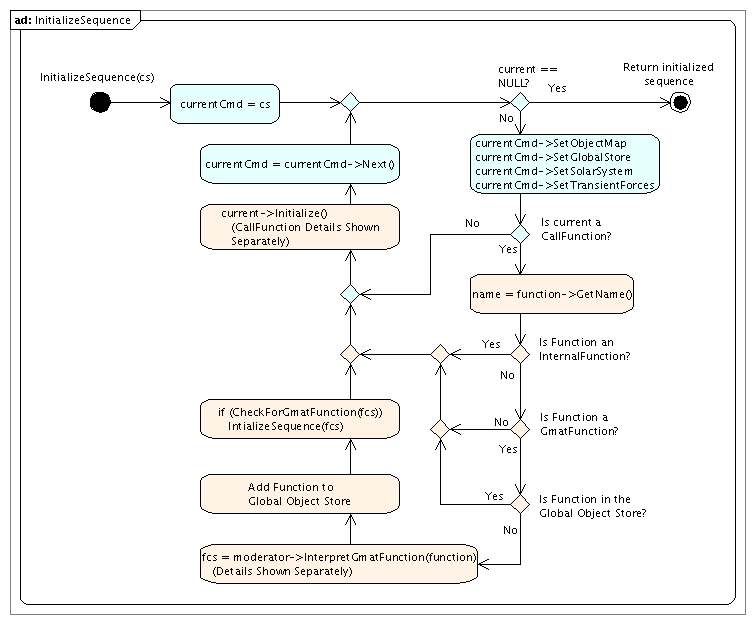
\includegraphics[378,312]{Images/InitializeSequence.png}
\caption{\label{figure:SequenceInit}Initialization of a Control Sequence in the Sandbox}
\end{center}
\end{figure}

\subsection{\label{section:SandboxInterruptPolling}Interrupt Polling During a Run}

\section{Usage and Modification}



\chapter{\label{chapter:FactoryManager}The Factory Manager}

The Factory Manager uses Factory classes to create objects for GMAT's model.  It takes creation
messages from the Moderator, passes those messages into the Factory designed to create the specific
type of object requested, and returns the created object to the Moderator.

This chapter describes the Factory Manager and introduces the Factory classes.  The Factory Manager
acts as the central junction into the Factory subsystem, managing Factories as they are created an
d registered, and routint creation requests to the specific Factory that knows how to create
a requested type of object.

Object creation is performed in a Factory derived from the Factory base class. An overview of the
Factory infrastructure is provided in Section~\ref{section:FactoryClasses}. Details about how you
use the Factory classes to extend GMAT can be found in Chapter~\ref{chapter:ExtendingGMAT}.

\section{Design Principles}

\subsection{Factory Manager Responsibilities}

\begin{enumerate}
\item Manages object creation for the engine.
\item Calls Factory classes to create objects.
\item Registers new Factories to support newly defined objects.
\item Provides a list of creatable object types.
\end{enumerate}

\subsection{The Abstract Factory Pattern, Factory Subclasses, and the Factory Manager}

\section{Design}

\begin{figure}[htb]
\begin{center}
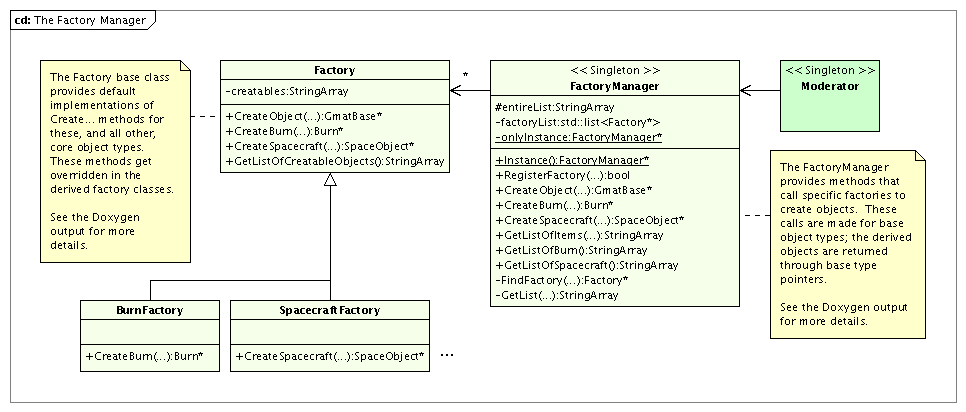
\includegraphics[460,197]{Images/TheFactoryManager.png}
\caption{The Factory Manager and Some Factories}
\label{figure:FactManClassDiagram}
\end{center}
\end{figure}



\subsection{Class Details}

\subsubsection{Class Attributes}

\subsection{\label{section:FactoryClassDesign}Design of the Factory Classes}

\subsubsection{Factory Details}


\section{Usage and Modification}



\chapter{\label{chapter:ConfigurationManager}The Configuration Manager}

User created objects are stored in a vector of object pointers called the configuration. The
Configuration Manager maintains this vector, provides access to the members, and adds new objects
to teh vector as they are created.  This chapter describes how the Configuration Manager performs
these tasks.

\section{Design Principles}

The Configuration Manager Does not initiate communications with any other components of GMAT.  It
responds to requests from the Moderator to store or retrieve components of the GMAT model.

\subsection{Configuration Manager Responsibilities}

The Configuration Manager plays a central role in object storage and retrieval for the model
elements.  It performs the following tasks:

\begin{enumerate}
\item Maintain the collection of configured objects used in the model.
\item Add new objects to the collection when they are created, ensuring that the new objects have
unique names.
\item Retrieve objects as they are needed.
\item Retrieve the list of stored objects, either by type or generically.
\item Clear the configuration in preparation for a new mission.
\end{enumerate}

\section{Design}

\subsection{Class Details}

\subsubsection{Class Attributes}

\section{Usage and Modification}


\chapter{\label{chapter:Publisher}The Publisher}

\section{Design Principles}

\subsection{Publisher Responsibilities}

\begin{enumerate}
\item Registers data Subscribers that receive data during a mission run.
\item Receives published data during a run and passes it to Subscribers.
\item Flushes data streams when needed.
\item Passes messages indicating state changes and other run information to the Subscribers.
\item Manages the subscriber list, adding or removing Subscribers as needed.
\end{enumerate}

\section{Design}

\subsection{Class Details}

\subsubsection{Class Attributes}

\section{Usage and Modification}


\part{Model Components}
\thispagestyle{empty}

%\part{Views and Interfaces}
%\thispagestyle{empty}

%\part{Utilities}
%\thispagestyle{empty}


%% $Id: GmatWorkFlow.tex,v 1.1 2008/01/31 18:04:16 dconway Exp $
\chapter{\label{chapter:WorkFlow}GMAT Work Flow}
\chapauthor{Darrel J. Conway}{Thinking Systems, Inc.}

This chapter describes, at a high level, the interactions of the objects in GMAT during a typical session.
\section{Configuring Objects}

\section{Running a Mission}

\section{Initialization}

\section{Execution}

\section{\label{section:InterfaceOverview}Interface Components}

% The interfaces to GMAT can be broken into interfaces with external system and interfaces with
% users.  The external interface component is used to provide an interface between GMAT and MATLAB.
% Other external systems may be interfaces to GMAT in future builds.  The internal interfaces are
% used to let the user control GMAT, either through custom text files called scripts, or through
% direct manipulation to objects managed in GMAT.  Figure~\ref{InterfacePackages} shows the
% main classes used to implement these interfaces.  The two major subdivisions are outlined here.
% Details of the design for these components can be found in chapters~\ref{chapter:ScriptRW},
% \ref{chapter:TheGui}, and \ref{chapter:ExternalInterfaces}.

%\begin{figure}[htb]
%\begin{center}
%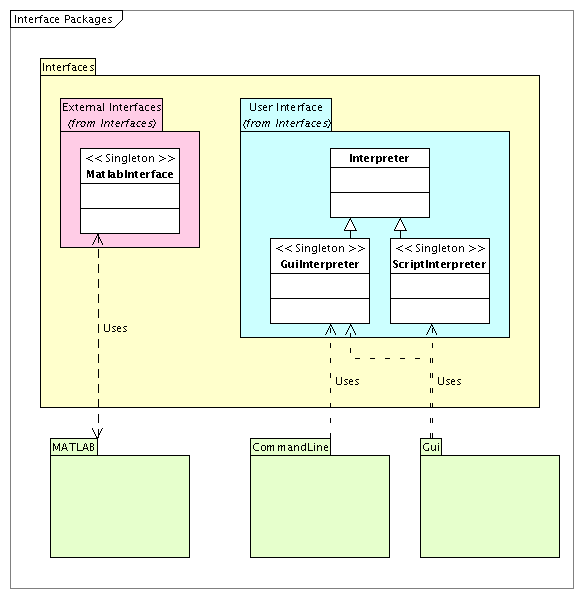
\includegraphics[420,430]{Images/InterfacePackages.png}
%\caption{\label{InterfacePackages}Interface Packages}
%\end{center}
%\end{figure}

\subsection{User Interfaces}

GMAT can be run from either a command line interface or a graphical user interface (GUI).  These
interfaces are connected to the core GMAT code through objects in the User Interface
portion of the Interface subsystem. The command line interface controls GMAT exclusively through
the singleton ScriptInterpreter  The GUI uses the ScriptInterpreter to read and write GMAT files
and to preview GMAT scripts, and the GuiInterpreter for other interactions with the internal GMAT
objects.

The command line interface provides minimal feedback during a run.  Users can use the command line
interface to execute GMAT scripts, either one at a time or in a batch mode.  The interface displays
status messages during the run, but provides no other feedback regarding the status of a script
run.  In batch mode, the interface runs multiple scripts sequentially based on the input from a
batch file.  Statistics regarding the success or failure of the individual scripts are collected
and displayed at the end of the run.

The graphical user interface is implemented using the wxWidgets GUI Library \cite{wxWidgets}.
It provides a rich development environment for the implementation of the user interface.  The GMAT
GUI is built on all three target platforms (Windows XP, MacIntosh OS X, and Linux) using the same
GUI code, with minimal customization for the different platforms.  The communications layer between
this library and core GMAT functionality is the GuiInterpreter.  Further information about the GUI
can be found in Chapter~\ref{chapter:TheGui}.

All scripting capabilities in GMAT are implemented using the ScriptInterpreter and its helper
classes.  This component is discussed in Chapter~\ref{chapter:ScriptRW}.  The GMAT scripting
language is documented in the \textbf{GMAT Mathematical Specifications and User's Guide}
\cite{mathSpec}, a companion volume to this document.

\subsection{External Interfaces}





%\part{Subsystem Designs}

% $Id: CoreClasses.tex,v 1.1 2008/01/31 18:04:16 dconway Exp $
\chapter{\label{chapter:CoreClasses}The GmatBase Class, Constants, and Defined Types}
\chapauthor{Darrel J. Conway}{Thinking Systems, Inc.}

This chapter documents GMAT's predefined data types, constants, and the core user classes used in
GMAT to implement the flight dynamics model.

\section{Defined Data Types}

GMAT uses the C++ type definition mechanism to define the data types shown in
Table~\ref{table:GmatDataTypes}.  These definitions, found in the gmatdefs.hpp header file, provide
a mechanism to generalize common data types and frequently used structures in the source code.

\begin{table}[H]
\begin{center}
\caption{\label{table:GmatDataTypes}Data Types Defined for GMAT}
\setlength\extrarowheight{2pt}
\begin{tabular}{|p{2in}|p{1.2in}|p{2.5in}|}
\hline
Defined typedef & Type Name & Description \\
\hline
\hline
double & Real & 8 byte float\\
int & Integer & 4 byte signed integer\\
unsigned char & Byte & 1 byte character\\
unsigned int & UnsignedInt & 4 byte unsigned integer\\
std::vector<Real> & RealArray & Vector of Reals\\
std::vector<Integer> & IntegerArray & Vector of signed integers\\
std::vector<UnsignedInt> & UnsignedIntArray & Vector of unsigned integers\\
std::vector<std::string> & StringArray & Vector of strings\\
std::vector<GmatBase*> & ObjectArray & Vector of GmatBase objects\\
std::vector<Gmat::ObjectType> & ObjectTypeArray & Vector of object type identifiers\\
\hline
\end{tabular}
\end{center}
\end{table}

\section{Error Handling in GMAT}

GMAT responds to critical anomalies in the configuration or other settings by throwing exceptions
reporting the error.  Every effort has been made to make GMAT's exception messages consistent and
informative.  Less serious anomalies may be reported through masseges passed as warnings to GMAT's
messaging system.  The classes implemented to support these two mechanisms are documented in
Chapter~\ref{chapter:Utilities}.

\section{\label{section:GmatBase}GmatBase}

The factory classes described in Chapter~\ref{chapter:Factories} are used to generate the resources
and Mission Control Sequence commands needed to simulate flight dynamics models.  The objects that
are generated in GMAT corresponding to these model elements are all instances of classes derived
from a base class named GmatBase.  The GmatBase class defines a common set of interfaces used to
build, configure, maintain, and store these elements.  This commonality of the interfaces into user
defined objects enforces consistency, simplifying common tasks that are performed on these objects.

Since understanding of the GmatBase is key to understanding how to work with the source code for
the model, this section of the document is written to thoroughly capture the contents of the class.
We'll begin by examining the class features in the following sections, and then provide some
information about how GMAT uses these features to set properties while reading and to serialize
model objects while writing objects to a text stream.

\subsection{GmatBase Attributes and Methods}

The features of GmatBase are broken into the class attributes and methods.  The method descriptions
are categorized into ??? subsections: (1) Constructors, Destructor, and Static Methods, (2) Object
Management Interfaces, (3) Interfaces Used for Scripting, the GUI, and External Communications, (4)
Class Attributes for Referenced and Owned Objects, (5) Class Attribute Management interfaces, and
(6 -- 9) sections for the interfaces into Reals, Integers, Strings, and other attribute types.

\subsubsection{\textit{Class Attributes}}

GmatBase contains data structures designed to manage the common elements shared by all of the
derived classes.  Configurable pieces of the derived classes are referred to as ``parameters'' in
the GmatBase code; hence the Integer attribute ``parameterCount'' reports the number of parameters
that can be accessed for instances of the derived class.  The attributes of GmatGase are described
here:

\begin{itemize}
\item \textbf{static Integer instanceCount}: Count of the number of GmatBase objects currently
instantiated.
\item \textbf{Integer parameterCount}: Count of the accessible parameters.
\item \textbf{std::string typeName}: Script string used or this class.
\item \textbf{std::string instanceName}: Name of the object -- empty if it is nameless.
\item \textbf{Gmat::ObjectType type}: Enumerated base type of the object.
\item \textbf{Integer ownedObjectCount}: Number of owned objects that belong to this instance.
\item \textbf{std::string generatingString}: Script string used to build the object.
\item \textbf{ObjectTypeArray objectTypes}: The list of generic types that this class extends.
\item \textbf{StringArray objectTypeNames}: The list types that this class extends, by name.
\item \textbf{ObjectTypeArray refObjectTypes}: The list of object types referenced by this class.
\item \textbf{StringArray refObjectNames}: The list of object names referenced by this class.
\item \textbf{bool callbackExecuting}: Flag indicating whether or not a Callback method is currently
executing.
\item \textbf{std::string errorMessageFormat}: The format string used when throwing error messages
for named objects.
\item \textbf{std::string errorMessageFormatUnnamed}: The format string used when throwing error
messages for unnamed objects.
\item \textbf{bool inMatlabMode}: Flag used to deterine if the current write is in Matlab mode.
\item \textbf{std::string commentLine}: String used to hold the comment line.
\item \textbf{std::string inlineComment}: String used to hold inline comment.
\item \textbf{StringArray attributeCommentLines}: String array used to hold the attribute comments.
\item \textbf{StringArray attributeInlineComments}: String array used to hold the attribute inline
comments.
\end{itemize}

\subsubsection{\textit{Constructor, Destructor, and Static Methods}}

GmatBase implements methods that override the default compiler-generated construction and
destruction capabilities, along with several class level utilities, as described below.

\paragraph{Default Methods}

C++ automatically defines four methods when a class is defined in code: a default constructor, a
copy constructor, a destructor, and an assignment operator.  Every user class in GMAT overrides
these methods to prevent generation of the default compiler versions.

\begin{itemize}
\item \textbf{GmatBase(Gmat::ObjectType typeId, const std::string \&typeStr, const std::string
\&nomme = "")}:  This is the default constructor for all GmatBase objects.
\item \textbf{virtual ~GmatBase() = 0}:  The base class destructor.  The destructor is set as
abstract, but it does have an implementation; designating it as abstract ensures that the compiler
will not allow GmatBase base class instances.
\item \textbf{GmatBase(const GmatBase \&a)}: The copy constructor.
\item \textbf{GmatBase\& operator=(const GmatBase \&a)}:  The assignment operator.
\end{itemize}

\paragraph{Static Methods}

The GmatBase class provides a mechanism to count object instances, provide numerical precision
setting data, and find object types and names through the following static class methods:

\begin{itemize}
\item \textbf{static Integer GetInstanceCount()}: Method to return the current number of
instantiated objects.
\item \textbf{static Integer GetDataPrecision()}: Returns the current precision setting used when
converting Real numbers into strings.
\item \textbf{static Integer GetTimePrecision()}: Returns the current precision setting used when
converting epoch data into strings.
\item \textbf{static std::string GetObjectTypeString(Gmat::ObjectType type)}: Method for getting
GMAT object type string.
\item \textbf{static Gmat::ObjectType GetObjectType(const std::string \&typeString)}: Method for
getting GMAT object type.
\end{itemize}

\subsubsection{\textit{Object Management Interfaces}}

GmatBase provides interfaces that are used to identify the object so that it can be accessed, and so
that other objects can find and connect to it.  These interfaces are described in this section.

\paragraph{Base Class Property Interfaces}

We'll begin by listing the interfaces that are used to retrieve information about the current
object.

\begin{itemize}
\item \textbf{virtual Gmat::ObjectType GetType() const}: Retrieves the core type of the object.
\item \textbf{inline std::string GetTypeName() const}: Retrieves the test description used for the
object type.
\item \textbf{inline std::string GetName() const}: Retrieves teh object's name.  Names in GMAT are
used to access objects in the Configuration; each user defined object that is stored in the
configuration is given a unique name.
\item \textbf{virtual bool SetName(const std::string \&who, const std::string \&oldName = "")}:
Renames the object.
\item \textbf{virtual Integer GetParameterCount() const}: Returns the number of parameters that can
be accessed for the object using the parameter interfaces, discussed below.
\item \textbf{bool IsOfType(Gmat::ObjectType ofType)}: Checks the object to see if it is derived
from the specified ObjectType.
\item \textbf{bool IsOfType(std::string typeDescription)}: Checks the object to see if it is derived
from the specified named type.
\end{itemize}

\paragraph{Overridable Interfaces}

The interfaces listed next are interfaces that are overrridden in the derived classes to provide
functionality as needed.

\begin{itemize}
\item \textbf{virtual GmatBase* Clone() const = 0}: Every GmatBase derived class that can be
instantiated must implement the Clone() method.  Clone() is used to copy objects from the
configuration into the Sandbox prior to the execution of the Mission Control Sequence.
\item \textbf{virtual void Copy(const GmatBase*)}: The Copy() method is provided so that objects
that need to copy data from other objects of the same class type can do so even when referenced
through GmatBase pointers.
\item \textbf{virtual bool Initialize()}: Objects that need to preform specific initialization
tasks override this method to perform those tasks.  The Sandbox calls the Initialize() method as
part of the Sandbox initialization process.
\item \textbf{virtual void SetSolarSystem(SolarSystem *ss)}: Objects that need access to GMAT's
current SolarSystem object override this method to set their SolarSystem pointer.
\item \textbf{virtual bool RequiresJ2000Body()}: Classes that need location data in the model use a
referenced body -- referred to as the J2000 body -- as the origin for spatial conversions.  Classes
that require this body override the RequiresJ2000Body method to return true from this call.
\item \textbf{virtual bool TakeAction(const std::string \&action, const std::string \&actionData =
"")}:  TakeAction() is a utility method that derived classes override to provide functionality that
cannot be implemented through basic parameter setting calls\footnote{One example of the use of the
TakeAction() can be found in the Spacecraft class.  The Spacecraft class uses TakeAction() to
manage attached tank and thruster objects.  Tanks and Thrusters are attached by name to the
Spacecraft instances during configuration, but the actual member objects are set during Sandbox
initialization through a call, ``TakeAction("SetupHardware");'', made to the Spacecraft object.}.
\item \textbf{virtual void FinalizeCreation()}: Performs initialization of GmatBase properties that
depend on the features of the derived classes.  Derived classes can touch some of the base class
properties -- the parameterCount, for example.  This method is called after the object creation
process is complete, so that any of the object's base-class properties can be updated to reflect
the object's actual properties.
\item \textbf{virtual std::string GetErrorMessageFormat()}: Returns the error message format string
used by the object.
\item \textbf{virtual void SetErrorMessageFormat(const std::string \&fmt)}: Updates the error
message format string used by the object.
\end{itemize}

\subsubsection{\textit{Interfaces Used for Scripting, the GUI, and External Communications}}

The interfaces used for scripting and callbacks are described in the following paragraphs.

\paragraph{General Purpose Interfaces}

All of the objects used in GMAT's model have the ability to produce text descriptions -- aka script
blocks -- sufficient to reproduce themselves and to incorporate text comments that help document the
intent of the setting selected by the user.  These interfaces are described here:

\begin{itemize}
\item \textbf{virtual const std::string GetCommentLine() const}: Returns the comment lines that
occur before the object definition or command line.
\item \textbf{virtual void SetCommentLine(const std::string \&comment)}: Sets the comment lines that
occur before the object definition or command line.
\item \textbf{virtual const std::string GetInlineComment() const}: Returns the comment that occurs
inline at the end of the object definition or command line.
\item \textbf{virtual void SetInlineComment(const std::string \&comment)}: Sets the comment that
occurs inline at the end of the object definition or command line.
\item \textbf{virtual const std::string GetAttributeCommentLine(Integer index)}: Returns any comment
that occurs before an attribute setting line.
\item \textbf{virtual void SetAttributeCommentLine(Integer index, const std::string \&comment)}:
Sets a comment that occurs before the attribute setting line.
\item \textbf{virtual const std::string GetInlineAttributeComment(Integer index)}: Returns the
comment that occurs at the end of an attribute setting line.
\item \textbf{virtual void  SetInlineAttributeComment(Integer index, const std::string \&comment)}:
Sets the comment that occurs at the end of an attribute setting line.
\item \textbf{virtual const std::string\& GetGeneratingString(Gmat::WriteMode mode =
Gmat::SCRIPTING, const std::string \&prefix = "", const std::string \&useName = "")}: Returns a
text string that can be used to regenerate the object.  See Section~\ref{section:GenStringModes} for
an explanation of the write modes.
\item \textbf{virtual StringArray GetGeneratingStringArray(Gmat::WriteMode mode = Gmat::SCRIPTING,
const std::string \&prefix = "", const std::string \&useName = "")}: Returns a string array that can
be used to regenerate the object.  See Section~\ref{section:GenStringModes} for an explanation of
the write modes.
\item \textbf{void CopyParameters(const GmatBase \&a)}: Copies the attributes from one object into
the current object.
\item \textbf{virtual void WriteParameters(Gmat::WriteMode mode, std::string \&prefix,
std::stringstream \&stream)}: Writes the parameter details for an object.  This method is called by
the GetGeneratingString methods to build the individual attribute lines needed to write configured
objects.
\item \textbf{void WriteParameterValue(Integer id, std::stringstream \&stream)}: Formats and
writes the attribute value portion of the attribute line.
\item \textbf{virtual void PrepCommentTables()}: A private method used to configure teh comment
tables so that they are sized correctly for the owning object.
\end{itemize}

\paragraph{Callback Interfaces}

Some GMAT classes are designed to communicate with external process through a basic callback
method.  These classes override the following methods to implement callbacks.

\begin{itemize}
\item \textbf{virtual bool ExecuteCallback()}: The method called from the external process to
execute a task in GMAT.
\item \textbf{virtual bool IsCallbackExecuting()}: Monitoring function used to determine if the
object is executing its callback method.
\item \textbf{virtual bool PutCallbackData(std::string \&data)}: Sends data from GMAT to the process
that is using the callback.
\item \textbf{virtual std::string GetCallbackResults()}: Retrieves the results of the callback.
\end{itemize}

\subsubsection{\textit{Class Attributes: Referenced and Owned Objects}}

Many of the user created objects need to interact with other model objects to correctly model the
spacecraft mission.  When an object uses the interfaces for a second named object that is stored in
the configuration, the second object is called a ``referenced object'' in this document. 
Occasionally an object will have, as a wholly owned, encapsulated member, another object.  These
internal member objects are called ``owned objects.''  The methods listed here are implemented to
work with the owned and referenced objects.

\begin{itemize}
\item \textbf{virtual std::string GetRefObjectName(const Gmat::ObjectType type) const}: Returns the
name of a referenced object of a specified type, of the object uses that type of referenced object.
\item \textbf{virtual const ObjectTypeArray\& GetRefObjectTypeArray()}: Returns an array of the
reference object types used by the current object.  Derived classes set the types in the
refObjectTypes attribute, which is returned from this call.
\item \textbf{virtual const StringArray\& GetRefObjectNameArray(const Gmat::ObjectType type)}:
Returns the reference object names used by the current object.  Derived classes override this
method to return the correct values.
\item \textbf{virtual bool SetRefObjectName(const Gmat::ObjectType type, const std::string
\&name)}: Sets the name of a referenced object.
\item \textbf{virtual bool RenameRefObject(const Gmat::ObjectType type, const std::string \&oldName,
const std::string \&newName)}: Resets the reference object name when the reference object is
renamed elsewhere.
\item \textbf{virtual GmatBase* GetRefObject(const Gmat::ObjectType type, const std::string
\&name)}: Returns the current reference object of specified type and name.
\item \textbf{virtual GmatBase* GetRefObject(const Gmat::ObjectType type, const std::string \&name,
const Integer index)}: Returns the current reference object when there are multiple objects of a
given type.  The referenced object is specified by type, name, and index.
\item \textbf{virtual bool SetRefObject(GmatBase *obj, const Gmat::ObjectType type, const
std::string \&name = "")}: Passes a referenced object's pointer into the object.
\item \textbf{virtual bool SetRefObject(GmatBase *obj, const Gmat::ObjectType type, const
std::string \&name, const Integer index)}: Passes a referenced object's pointer into the object for
use in an array of referenced objects.
\item \textbf{virtual ObjectArray\& GetRefObjectArray(const Gmat::ObjectType type)}: Retrieves an
array of referenced objects by type.
\item \textbf{virtual ObjectArray\& GetRefObjectArray(const std::string\& typeString)}: Retrieves an
array of referenced objects by type name.
\item \textbf{virtual Integer GetOwnedObjectCount()}: Retrieves the number of owned objects
contained in the object.
\item \textbf{virtual GmatBase* GetOwnedObject(Integer whichOne)}: Retrieves teh owned objects by
index into the owned object array.
\end{itemize}

\subsubsection{\textit{Class Attribute Accessors: Parameter Management}}

All of the attributes of the GmatBase classes that are accessible directly by users have associated
descriptions, ID numbers, and types.  When attributes have these features, they will be referred to
as parameters in this chapter.  Classes can have other attributes that are not directly accessible
by users.

The parameters that are reported when an object is serialized are identified and read and
write enabled parameters; those that are not contained in the serialization are nominally identified
as read only, though the base class does not enforce read-only nature on those parameters.  Classes
that need strict read-only enforcement implement that nature in the parameter access methods.

The parameter management interfaces are described here:

\begin{itemize}
\item \textbf{virtual std::string GetParameterText(const Integer id) const}: Returns the text
string associated with the parameter ID input into the method.
\item \textbf{virtual Integer GetParameterID(const std::string \&str) const}: Returns the ID
associated with a parameter's description.
\item \textbf{virtual Gmat::ParameterType GetParameterType(const Integer id) const}: Returns
the parameter type for the specified ID.
\item \textbf{virtual std::string GetParameterTypeString(const Integer id) const}: Returns the
parameter type string for the input parameter ID.
\item \textbf{virtual bool IsParameterReadOnly(const Integer id) const}: Returns true if the
parameter, identified by parameter ID, is read-only.  Derived classes override this method to
identify read-only parameters.
\item \textbf{virtual bool IsParameterReadOnly(const std::string \&label) const}: Returns true if
the parameter, identified by parameter name, is read-only.  Derived classes override this method to
identify read-only parameters.
\end{itemize}

\subsubsection{Static Members Used with Attributes}

GmatBase includes several class-level (static) members used to simplify parameter access methods.
These members are specified in the following tables.

\paragraph{String Definitions for Attributes}

The arrays shown in Table~\ref{table:PropertyTypesAndLabels} provide text strings for each of
GMAT's defined data types and object types.  These strings are used to identify types in a human
readable format.

\begin{table}[H]
\begin{center}
\caption{\label{table:PropertyTypesAndLabels}Arrays Holding Defined Type Names}
\setlength\extrarowheight{2pt}
\begin{tabular}{|p{1.35in}|p{1.75in}|p{2.7in}|}
\hline
Type & Array Name & Purpose \\
\hline
\hline
static const std::string & PARAM\_TYPE\_STRING[] & String mappings for the GMAT data types\\
static const std::string & OBJECT\_TYPE\_STRING[] & String mappings for the GMAT object types\\
\hline
\end{tabular}
\end{center}
\end{table}

\paragraph{Constants for Undefined Values}

Occasionally GMAT objects need an initial value for attribute initialization when that value is not
yet available.  The static constants shown in Table~\ref{table:GmatbaseUndefinedValues} provide
these initial values.

\begin{table}[H]
\begin{center}
\caption{\label{table:GmatbaseUndefinedValues}Constants Holding Undefined Values}
\setlength\extrarowheight{2pt}
\begin{tabular}{|p{1.1in}|p{3.1in}|p{1.8in}|}
\hline
Type & Variable Name & Value \\
\hline
\hline
const Real & REAL\_PARAMETER\_UNDEFINED & -987654321.0123e-45\\
const Integer & INTEGER\_PARAMETER\_UNDEFINED & -987654321\\
const UnsignedInt & UNSIGNED\_INT\_PARAMETER\_UNDEFINED & 987654321\\
const std::string & STRING\_PARAMETER\_UNDEFINED & "STRING\-\_PARAMETER\-\_UNDEFINED"\\
const Rvector & RVECTOR\_PARAMETER\_UNDEFINED & A 1-element Rvector, initialized to
REAL\-\_PARAMETER\-\_UNDEFINED\\
const Rmatrix & RMATRIX\_PARAMETER\_UNDEFINED & A 1-by-1 Rmatrix, initialized to
REAL\-\_PARAMETER\-\_UNDEFINED\\
\hline
\end{tabular}
\end{center}
\end{table}

The following sections describe the interfaces used to access the parameters.  These methods are
type specific; the parameter has to have the type accosiated with teh method in order to return a
valid value.

\subsubsection{\textit{Class Attributes: Real Number Interfaces}}

GmatBase objects support the following interfaces into Real number attributes:

\begin{itemize}
\item \textbf{virtual Real GetRealParameter(const Integer id) const}: Retrieves the Real value of
the parameter with the specified ID.
\item \textbf{virtual Real SetRealParameter(const Integer id,const Real value)}: Sets the Real
value of the parameter with the specified ID.
\item \textbf{virtual Real GetRealParameter(const Integer id, const Integer index) const}: Retrieves
the Real value of a parameter stored in a vector, where the vector is identified by the specified
ID, and the requested element has the specified index.
\item \textbf{virtual Real GetRealParameter(const Integer id, const Integer row, const Integer
col) const}: Retrieves the Real value of a parameter stored in an array, where the array is
identified by the specified ID, and the requested element is located in the specified row and
column.
\item \textbf{virtual Real SetRealParameter(const Integer id, const Real value, const Integer
index)}: Sets the Real value of a parameter stored in a vector, where the vector is identified by
the specified ID, and the requested element has the specified index.
\item \textbf{virtual Real SetRealParameter(const Integer id, const Real value, const Integer row,
const Integer col)}: Sets the Real value of a parameter stored in an array, where the array is
identified by the specified ID, and the requested element is located in the specified row and
column.
\item \textbf{virtual Real GetRealParameter(const std::string \&label) const}: Retrieves the Real
value of the parameter with the text label.
\item \textbf{virtual Real SetRealParameter(const std::string \&label, const Real value)}: Sets the
Real value of the parameter with the specified text label.
\item \textbf{virtual Real GetRealParameter(const std::string \&label, const Integer index)
const}: Retrieves the Real value of a parameter stored in a vector, where the vector is identified
by the specified text label, and the requested element has the specified index.
\item \textbf{virtual Real SetRealParameter(const std::string \&label, const Real value, const
Integer index)}: Sets the Real value of a parameter stored in a vector, where the vector is
identified by the specified text label, and the requested element has the specified index.
\item \textbf{virtual Real GetRealParameter(const std::string \&label, const Integer row,  const
Integer col) const}: Retrieves the Real value of a parameter stored in an array, where the array is
identified by the specified text label, and the requested element is located in the specified row
and column.
\item \textbf{virtual Real SetRealParameter(const std::string \&label, const Real value, const
Integer row, const Integer col)}: Sets the Real value of a parameter stored in an array, where the
array is identified by the specified text label, and the requested element is located in the
specified row and column.
\item \textbf{virtual const Rvector\& GetRvectorParameter(const Integer id) const}: Retrieves a
vector of Real data, contained in an Rvector instance, with the specified ID.
\item \textbf{virtual const Rvector\& SetRvectorParameter(const Integer id, const Rvector
\&value)}: Sets a vector of Real data, contained in an Rvector, with the specified ID.
\item \textbf{virtual const Rmatrix\& GetRmatrixParameter(const Integer id) const}: Retrieves an
array of Real data, contained in an Rmatrix instance, with the specified ID.
\item \textbf{virtual const Rmatrix\& SetRmatrixParameter(const Integer id, const Rmatrix
\&value)}: Sets an array of Real data, contained in an Rmatrix instance, with the specified ID.
\item \textbf{virtual const Rvector\& GetRvectorParameter(const std::string \&label) const}:
Retrieves a vector of Real data, contained in an Rvector instance, with the specified text label.
\item \textbf{virtual const Rvector\& SetRvectorParameter(const std::string \&label, const Rvector
\&value)}: Sets a vector of Real data, contained in an Rvector, with the specified text label.
\item \textbf{virtual const Rmatrix\& GetRmatrixParameter(const std::string \&label) const}:
Retrieves an array of Real data, contained in an Rmatrix instance, with the specified text label.
\item \textbf{virtual const Rmatrix\& SetRmatrixParameter(const std::string \&label, const Rmatrix
\&value)}: Sets an array of Real data, contained in an Rmatrix instance, with the specified text
label.
\end{itemize}

\subsubsection{\textit{Class Attributes: Integer Interfaces}}

The access methods used for integer parameters -- both signed and unsigned -- are listed here:

\begin{itemize}
\item \textbf{virtual Integer GetIntegerParameter(const Integer id) const}: Retrieves the Integer
value of the parameter with the specified ID.
\item \textbf{virtual Integer SetIntegerParameter(const Integer id, const Integer value)}: Sets the
Integer value of the parameter with the specified ID.
\item \textbf{virtual Integer GetIntegerParameter(const Integer id, const Integer index) const}:
Retrieves the Integer value of a parameter stored in a vector, where the vector is identified by the
specified ID, and the requested element has the specified index.
\item \textbf{virtual Integer SetIntegerParameter(const Integer id, const Integer value, const
Integer index)}: Sets the Real value of a parameter stored in a vector, where the vector is
identified by the specified ID, and the requested element has the specified index.
\item \textbf{virtual UnsignedInt GetUnsignedIntParameter(const Integer id) const}: Retrieves the
unsigned Integer value of the parameter with the specified ID.
\item \textbf{virtual UnsignedInt SetUnsignedIntParameter(const Integer id, const UnsignedInt
value)}: Sets the unsigned Integer value of the parameter with the specified ID.
\item \textbf{virtual UnsignedInt GetUnsignedIntParameter(const Integer id, const Integer index)
const}: Retrieves the unsigned Integer value of a parameter stored in a vector, where the vector is
identified by the specified ID, and the requested element has the specified index.
\item \textbf{virtual UnsignedInt SetUnsignedIntParameter(const Integer id, const UnsignedInt
value, const Integer index)}: Sets the unsigned Integer value of a parameter stored in a vector,
where the vector is identified by the specified ID, and the requested element has the specified
index.
\item \textbf{virtual const UnsignedIntArray\& GetUnsignedIntArrayParameter(const Integer id)
const}: Retrieves an array of unsigned Integers identified by the specified ID.
\item \textbf{virtual Integer GetIntegerParameter(const std::string \&label) const}: Retrieves an
Integer parameter identified by the specified text label.
\item \textbf{virtual Integer SetIntegerParameter(const std::string \&label, const Integer
value)}: Sets an Integer parameter identified by the specified text label
\item \textbf{virtual Integer GetIntegerParameter(const std::string \&label, const Integer index)
const}: Retrieves the Integer value of a parameter stored in a vector, where the vector is
identified by the specified text label and the requested element has the specified index.
\item \textbf{virtual Integer SetIntegerParameter(const std::string \&label, const Integer value,
const Integer index)}: Sets the Integer value of a parameter stored in a vector, where the vector is
identified by the specified text label and the requested element has the specified index.
\item \textbf{virtual UnsignedInt GetUnsignedIntParameter(const std::string \&label) const}:
Retrieves the unsigned Integer value of a parameter identified by a text label.
\item \textbf{virtual UnsignedInt SetUnsignedIntParameter(const std::string \&label, const
UnsignedInt value)}: Sets the unsigned Integer value of a parameter identified by a text label.
\item \textbf{virtual UnsignedInt GetUnsignedIntParameter(const std::string \&label, const Integer
index) const}: Retrieves the unsigned Integer value of a parameter stored in a vector, where the
vector is identified by a text label, and the requested element has the specified index.
\item \textbf{virtual UnsignedInt SetUnsignedIntParameter(const std::string \&label, const
UnsignedInt value, const Integer index)}: Sets the unsigned Integer value of a parameter stored in a
vector, where the vector is identified by a text label, and the requested element has the specified
index.
\item \textbf{virtual const UnsignedIntArray\& GetUnsignedIntArrayParameter(const std::string
\&label) const}: Retrieves an array of unsigned Integers identified by a text label.
\end{itemize}

\subsubsection{\textit{Class Attributes: String Interfaces}}

String interfaces are used to set reference object names, along with other textual data used inside
of the GmatBase objects.  The string interfaces into GmatBase parameters are described here:

\begin{itemize}
\item \textbf{virtual std::string GetStringParameter(const Integer id) const}: Retrieves the
string value of the parameter with the specified ID.
\item \textbf{virtual bool SetStringParameter(const Integer id, const std::string \&value)}:
Sets the string value of the parameter with the specified ID.
\item \textbf{virtual std::string GetStringParameter(const Integer id, const Integer index)
const}: Retrieves a string from a vector of strings, where the vector has the specified ID and the
retrieved string is in the vector element identified by index.
\item \textbf{virtual bool SetStringParameter(const Integer id, const std::string \&value, const
Integer index)}: Sets a string in a vector of strings, where the vector has the specified ID
and the input string is placed in the vector element identified by index.
\item \textbf{virtual std::string GetStringParameter(const std::string \&label) const}: Retrieves
the string value of the parameter with the specified text label.
\item \textbf{virtual bool SetStringParameter(const std::string \&label, const std::string
\&value)}: Sets the string value of the parameter with the specified text label.
\item \textbf{virtual std::string GetStringParameter(const std::string \&label, const Integer
index) const}: Retrieves a string from a vector of strings, where the vector has the specified text
label and the retrieved string is in the vector element identified by index.
\item \textbf{virtual bool SetStringParameter(const std::string \&label, const std::string
\&value, const Integer index)}: Sets a string in a vector of strings, where the vector has the
specified text label and the input string is placed in the vector element identified by the
specified index.
\item \textbf{virtual const StringArray\& GetStringArrayParameter(const std::string \&label)
const}: Retrieves a vector of strings stored in the vector associated with a text label.
\item \textbf{virtual const StringArray\& GetStringArrayParameter(const std::string \&label, const
Integer index) const}: Retrieves a vector of strings from a vector of string arrays identified by
a text label.  The retrieved vector is identified by index into the vector of string arrays.
\item \textbf{virtual const StringArray\& GetStringArrayParameter(const Integer id) const}:
Retrieves a vector of strings stored in the parameter associated with an ID.
\item \textbf{virtual const StringArray\& GetStringArrayParameter(const Integer id, const Integer
index) const}: Retrieves a vector of strings from a vector of string arrays identified by ID.  The
retrieved vector is identified by index into the vector of string arrays.
\end{itemize}

\subsubsection{\textit{Class Attributes: Boolean Interfaces}}

GmatBase supports two types of boolean parameters: standard C++ bool values and a sttring version
of boolean data, set to either the string ``On'' or ``Off.''  The interfaces implemented into these
parameters is presented here:

\begin{itemize}
\item \textbf{virtual bool GetBooleanParameter(const Integer id) const}: Retrieves the boolean value
of the parameter with the specified ID.
\item \textbf{virtual bool SetBooleanParameter(const Integer id, const bool value)}: Sets the
boolean value of the parameter with the specified ID.
\item \textbf{virtual bool GetBooleanParameter(const Integer id, const Integer index) const}:
Retrieves a boolean from a vector of booleans, where the vector has the specified ID and the
retrieved boolean is in the vector element identified by index.
\item \textbf{virtual bool SetBooleanParameter(const Integer id, const bool value, const Integer
index)}: Sets a boolean into a vector of booleans, where the vector has the specified ID and
the input boolean is in the vector element identified by index.
\item \textbf{virtual bool GetBooleanParameter(const std::string \&label) const}: Retrieves the
boolean value of the parameter with the specified text label.
\item \textbf{virtual bool SetBooleanParameter(const std::string \&label, const bool value)}: Sets
the boolean value of the parameter with the specified text label.
\item \textbf{virtual bool GetBooleanParameter(const std::string \&label, const Integer index)
const}: Retrieves a boolean from a vector of booleans, where the vector has the specified text label
and the retrieved boolean is in the vector element identified by index.
\item \textbf{virtual bool SetBooleanParameter(const std::string \&label, const bool value, const
Integer index)}: Sets a boolean into a vector of booleans, where the vector has the specified text
label and the input boolean is in the vector element identified by index.
\item \textbf{virtual std::string GetOnOffParameter(const Integer id) const}: Retrieves the state
value (``On'' or ``Off'') of the parameter with the specified ID.
\item \textbf{virtual bool SetOnOffParameter(const Integer id, const std::string \&value)}: Sets the
state value (``On'' or ``Off'') of the parameter with the specified ID.
\item \textbf{virtual std::string GetOnOffParameter(const std::string \&label) const}: Retrieves the
state value (``On'' or ``Off'') of the parameter with the specified text label.
\item \textbf{virtual bool SetOnOffParameter(const std::string \&label, const std::string
\&value)}: Sets the state value (``On'' or ``Off'') of the parameter with the specified text label.
\end{itemize}

\subsection{Setting GmatBase Properties}

\begin{figure}[htb]
\begin{center}
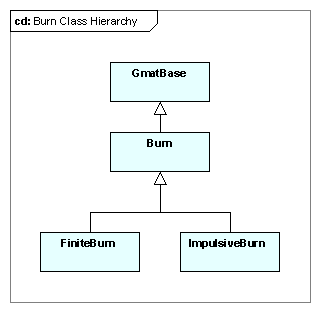
\includegraphics[160,155]{Images/BurnClassHierarchy.png}
\caption{\label{figure:BurnClassOverview}Class Hierarchy for Gmat's Burn Resources}
\end{center}
\end{figure}

The somewhat tedious descriptions provided above show the interfaces into parameters for the
configured objects in a static format.  The next two sections show in a bit more detail how these
interfaces are used to set parameters and to construct a serialized version of a GmatBase object. 
We'll begin with an example setting several properties on an ImpulsiveBurn object.  The class
hierarchy for ImpulsiveBurns is shown in Figure~\ref{figure:BurnClassOverview}.

\lstset{numbers=left,firstnumber=1,escapeinside={(*@}{@*)}}
\begin{lstlisting}[caption={Script Listing for an ImpulsiveBurn},
label={listing:ImpulsiveBurn}]
Create ImpulsiveBurn Burn1;

(*@\label{line:IBScriptFirstParameter}@*)Burn1.Origin = Earth;
Burn1.Axes = VNB;
Burn1.VectorFormat = Cartesian;
Burn1.Element1 = 3.16;
Burn1.Element2 = 0;
(*@\label{line:IBScriptLastParameter}@*)Burn1.Element3 = 0;
\end{lstlisting}
\lstset{numbers=none}

The serialized text -- that is, the scripting -- for an ImpulsiveBurn object is shown in
Listing~\ref{listing:ImpulsiveBurn}.  As can be seen on
lines~\ref{line:IBScriptFirstParameter}~--~\ref{line:IBScriptLastParameter} in this listing,
ImpulsiveBurn objects have six accessible parameters that users can manipulate: the Origin of the
burn (``Origin''), the Axes used to orient the burn in space (``Axes''), a format defining how the
burn is written relative to these axes (``VectorFormat''), and the three components necessary to
define the delta-V that this burn models (``Element1'', ``Element2'', and ``Element3'').

When GMAT reads a script containing these lines, it creates a new ImpulsiveBurn object named Burn1
and sets the values found in the script into the associated parameters on the object.  The object
creation process was described in Section~\ref{section:ObjectCreation}. 
Figure~\ref{figure:SettingBurnParameters} shows the calls made to the new object to set the
parameter values.  The steps shown in this figure are straightforward:

\begin{enumerate}
\item \textbf{Call Burn1->GetParameterType(``Origin'')} Determines that the ``Origin'' parameter
is a string.
\item \textbf{Call Burn1->SetStringParameter(``Origin'', ``Earth'')} Sets the ``Origin''
parameter to the string ``Earth''.
\item \textbf{Call Burn1->GetParameterType(``Axes'')} Determines that the ``Axes'' parameter
is a string.
\item \textbf{Call Burn1->SetStringParameter(``Axes'', ``VNB'')} Sets the ``Axes''
parameter to the string ``VNB'', denoting that the burn is specified in the
Velocity-Normal-Binormal representation.
\item \textbf{Call Burn1->GetParameterType(``VectorFormat'')} Determmines that the ``VectorFormat''
parameter is a string.
\item \textbf{Call Burn1->SetStringParameter(``VectorFormat'', ``Cartesian'')} Sets the
``VectorFormat'' parameter to the string ``Cartesian''.
\item \textbf{Call Burn1->GetParameterType(``Element1'')} Determines that the ``Element1'' parameter
is a Real number.
\item \textbf{Call Burn1->SetRealParameter(``Element1'', 3.16)} Sets the ``Element1''
parameter to the value 3.16.
\item \textbf{Call Burn1->GetParameterType(``Element2'')} Determines that the ``Element2'' parameter
is a Real number.
\item \textbf{Call Burn1->SetRealParameter(``Element2'', 0)} Sets the ``Element2''
parameter to the value 0.0.
\item \textbf{Call Burn1->GetParameterType(``Element3'')} Determines that the ``Element3'' parameter
is a Real number.
\item \textbf{Call Burn1->SetRealParameter(``Element3'', 0)} Sets the ``Element3''
parameter to the value 0.0.
\end{enumerate}

\begin{figure}[htb]
\begin{center}
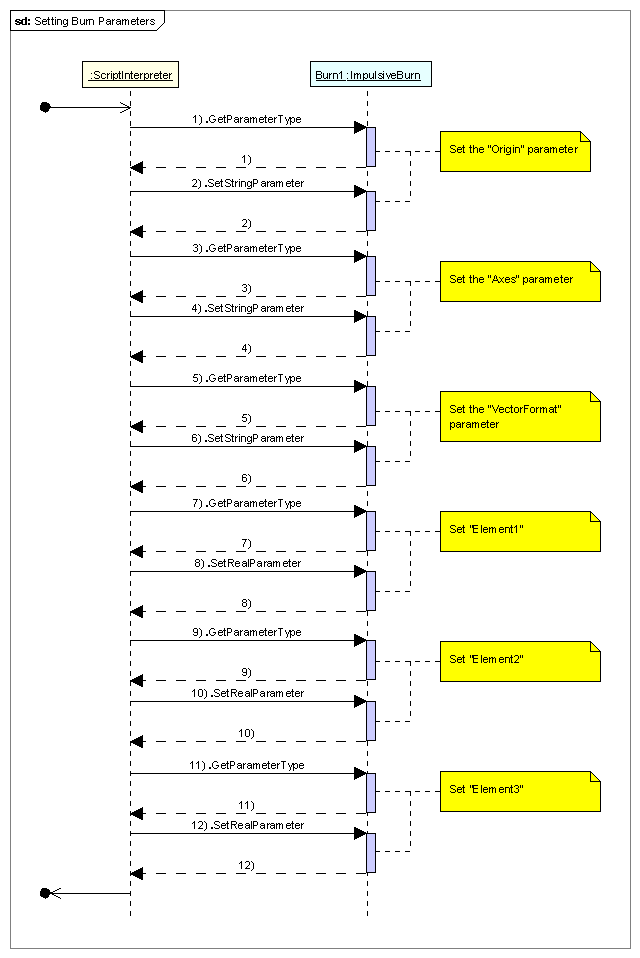
\includegraphics[241,416]{Images/SettingBurnParameters.png}
\caption{\label{figure:SettingBurnParameters}Parameter Setting for
Listing~\ref{listing:ImpulsiveBurn}}
\end{center}
\end{figure}

\subsection{Serializing GmatBase Objects}

Objects are written to text using the GetGeneratingString() method.  GetGeneratingString can
serialize objects this way for several purposes: to write an object to a script file, to pass the
object to MATLAB or a MATLAB compatible external process, or in some cases to generate data used
for the generation of an ephemeris file.  The mode used for the serialization is determined using a
setting on the call to GetGeneratingString().  That setting, the write mode, is set using the
WriteMode enumeration.

The following paragraphs describe the process followed when performing serialization of GmatBase
objects.  We begin with a brief description of the WriteMode enumeration, followed by a detailed
description of the call to GetGeneratingString that serializes an object for scripting purposes,
and conclude with a description of the differences encountered when serializing an object for
MATLAB.

\subsubsection{\label{section:GenStringModes}The WriteMode Enumeration}

Table~\ref{table:WriteModeEnum} shows the modes available to the GetGeneratingString methods for
serialization of objects in GMAT.  These modes are defined in an enumeration, WriteMode, contained
in the Gmat namespace.  GMAT uses the SCRIPTING mode as the default write mode, generating text
strings that are designed to work with the script interpreter classes when saving a model to a
script file.

\begin{table}[htb]
\begin{center}
\caption{\label{table:WriteModeEnum}The WriteMode Enumeration}
\setlength\extrarowheight{2pt}
\begin{tabular}{|p{1.7in}|p{4in}|}
\hline
Identifier & Description \\
\hline
\hline
SCRIPTING & The mode used when writing an object as it appears in GMAT's script files.\\
SHOW\_SCRIPT & Similar to the SCRIPTING mode, the SHOW\_SCRIPT mode serializes an object as it
would appear in a script file.  The SHOW\_SCRIPT mode does not guarantee that the resulting text
is indented as it would be in a written script.\\
OWNED\_OBJECT & OWNED\_OBJECT mode is used to serialize the objects owned by an object that is
being written to the text stream.\\
MATLAB\_STRUCT & Generates the serialed object as a MATLAB structuire, so that the object can be
passed into MATLAB for external processing.\\
EPHEM\_HEADER & Generates a string used in GMAT's output ephemeris headers.\\
\hline
\end{tabular}
\end{center}
\end{table}

\subsubsection{Writing to Script}

\begin{figure}[htb]
\begin{center}
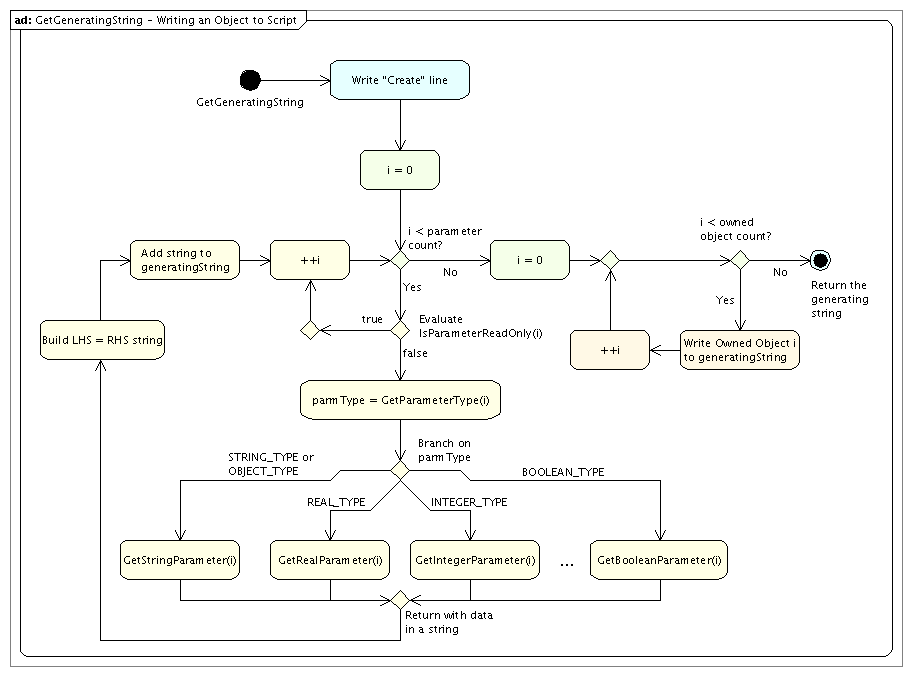
\includegraphics[385,338]{Images/GetGeneratingStringWritinganObjecttoScript.png}
\caption{\label{figure:GetGeneratingStringDetails}Flow in the GetGeneratingString() Method}
\end{center}
\end{figure}

Figure~\ref{figure:GetGeneratingStringDetails} shows the procedure followed when the
GetGeneratingString() method is called on a configured object to write that object in script
format\footnote{GetGeneratingString() can be overridden by the derived classes.  The description
provided here is the default behavior.  Command classes, in particular, always override this
method so that the command specific scripting can be generated.}. The process starts by clearing the
current generatingString attribute, and then writing the initial Create line to it.  Objects
without any parameters or owned objects are finished at this point, and simply return the resulting
string, following the path shown in green in the figure.

If the object's parameter count is not zero, then the GetGeneratingString() method calls the
WriteParameters() method, which adds text lines to the generatingString for each parameter that is
writable.  This process is shown in yellow in the figure.  The process starts by initializing an
index into the parameter list for the object.  This index is used to loop through the parameters
for the object.  For each parameter, the code calls the IsParameterReadOnly() method to determine
 if the parameter should be written to teh generating string.  If the parameter is not read only,
the current value of the parameter is sent into a string in the WriteParameterValue() method.  The
WriteParameterValue method determines the type of the parameter, and calls the corresponding access
method to retrieve the value and place it into a string.  This string is returned to the
WriteParameters() method for use as the right hand side of the text string setting the parameter's
value.  The parameter setting string is then build, using a call to GetParameterText() for the left
side of the parameter setting string and the string returned from the call to WriteParameterValue()
for the right side of the parameter setting string.  The resulting string is added to the
generating string, and the parameter index is incremented to move to the next parameter.

Once the parameter index has iterated through all of the parameters, the call to WriteParameters()
returns control to the GetGeneratingString() method.  GetGeneratingString() resets its index, and
then checks for owned objects.  If there are any owned objects, each owned object writes its data
to the generating string, following the process shown in orange in the figure.  Owned objects write
their data through calls to their GetGeneratingString() methods, with the write mode set to teh
OWNED\_OBJECT mode.  After all of the owned objects have been written, the generating string is
returned to the caller, completing the serialization process.

Listing~\ref{listing:CoordinateSystem} shown an example of the output generated when a coordinate
system is written to script.

\lstset{numbers=left,firstnumber=1,escapeinside={(*@}{@*)}}
\begin{lstlisting}[caption={Script Listing for a Coordinate System},
label={listing:CoordinateSystem}]
Create CoordinateSystem SunPointingCS;
GMAT SunPointingCS.Origin = DefaultSC;
GMAT SunPointingCS.Axes = ObjectReferenced;
GMAT SunPointingCS.UpdateInterval = 60;
GMAT SunPointingCS.OverrideOriginInterval = false;
GMAT SunPointingCS.XAxis = R;
GMAT SunPointingCS.ZAxis = N;
GMAT SunPointingCS.Primary = DefaultSC;
GMAT SunPointingCS.Secondary = Sun;
\end{lstlisting}
\lstset{numbers=none}

\subsubsection{Writing to MATLAB}

The process followed when an object is serialized for export to MATLAB is the same as that shown in
the sequence diagram for writing to script, Figure~\ref{figure:GetGeneratingStringDetails}.  The
key differences between the processes are contained in the details of the strings generated.  When
an object is serialized for MATLAB, the Create line is omitted.  The ``GMAT'' preface used for
parameter strings in SCRIPTING mode is also omitted, and strings are enclosed in single quotes to
conform to MATLAB's syntax.  Listing~\ref{listing:MATLABCoordinateSystem} shows the resulting
serailized version of the same coordinate system as was shown in the script serialization example,
above.

\lstset{numbers=left,firstnumber=1,escapeinside={(*@}{@*)}}
\begin{lstlisting}[caption={MATLAB Listing for a Coordinate System},
label={listing:MATLABCoordinateSystem}]
SunPointingCS.Origin = 'DefaultSC'
SunPointingCS.Axes = 'ObjectReferenced'
SunPointingCS.UpdateInterval = 60
SunPointingCS.OverrideOriginInterval = false
SunPointingCS.XAxis = 'R'
SunPointingCS.ZAxis = 'N'
SunPointingCS.Primary = 'DefaultSC'
SunPointingCS.Secondary = 'Sun'
\end{lstlisting}
\lstset{numbers=none}

\subsection{GmatBase Derivatives}

\begin{figure}[htb]
\begin{center}
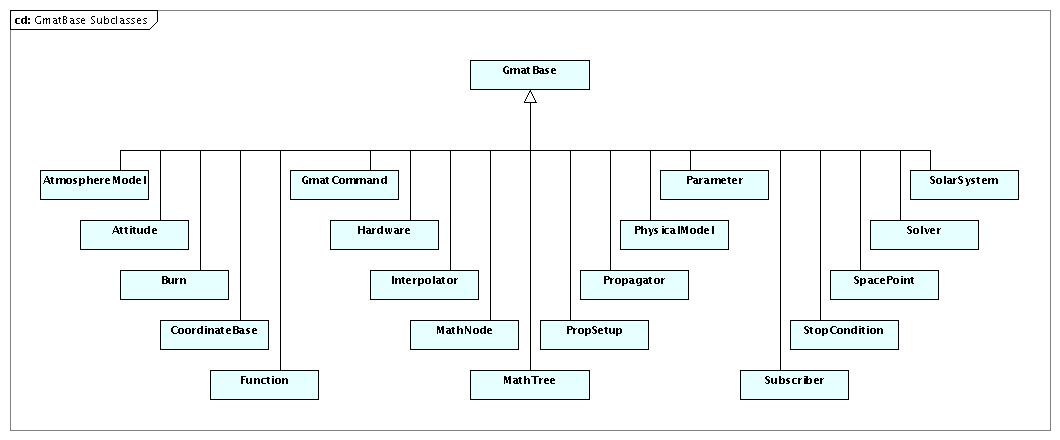
\includegraphics[455,185]{Images/GmatBaseSubclasses.png}
\caption{\label{figure:GmatBaseSubclasses}Classes Derived from GmatBase}
\end{center}
\end{figure}

Figure~\ref{figure:GmatBaseSubclasses} shows the classes derived from GmatBase.  These classes are
presented more fully in other chapters of this document.  Here is a brief description of each, with
cross references to the chapters that provide the detailed descriptions:

\begin{description}
\item \textbf{AtmosphereModel} Models the Atmosphere for bodies in the SolarSystem.  The
AtmosphereModel classes are used to determine atmospheric densities in GMAT's Drag models.  Force
modeling is described in Chapter~\ref{chapter:ForceModel}.
\item \textbf{Attitude} The base class for attitude modeling in GMAT.  Attitude modeling is
described in Chapter~\ref{chapter:Attitude}.
\item \textbf{Burn} The base class for burn modeling.  The Burn class contains the elements common
to finite and impulsive burns.  The burn classes and other components used in maneuver modeling are
described in Chapter~\ref{chapter:Maneuvers}.
\item \textbf{CoordinateBase} The base class for coordinate system modeling.  GMAT provides a quite
extensive system of coordinate system models, described in Chapter~\ref{chapter:CoordinateSystems}.
\item \textbf{Function} The base class for internal and external functions, described in
Chapter~\ref{chapter:Functions}.
\item \textbf{GmatCommand} The base class for the commands in the Mission Control Sequence. 
Commands are described in Chapters~\ref{chapter:Commands} and~\ref{chapter:SpecificCommands}.
\item \textbf{Hardware} The base class for hardware elements that can be attached to other objects. 
Fuel tanks, thrusters, sensors, and antennae are all derived from this class.  THe Hardware classes
are described in Chapter~\ref{chapter:Hardware}.
\item \textbf{Interpolator} The base class for the numerical interpolaters.  The interpolators are
described in Chapter~\ref{chapter:Utilities}.
\item \textbf{MathNode} GMAT supports mathematics performed as part of the Mission Control
Sequence. Mathematical expressions are decomposed into a tree structure for evaluation.  The
MathNode class is used for the nodes in this tree structure, as is described in
Chapter~\ref{chapter:InlineMath}.
\item \textbf{MathTree} MathTree objects are used as containers for inline mathematicas in GMAT's
Mission Control Sequence, as is described in Chapter~\ref{chapter:InlineMath}.
\item \textbf{Parameter} GMAT can calculate many different properties that are useful for analyzing
spacecraft missions.  The code that implements these calculations is derived from the Parameter
class, described in Chapter~\ref{chapter:Parameters}.
\item \textbf{PhysicalModel} The PhysicalModel class is the base class for all of the forces used
in GMAT's propagators.  Force mdodeling is described in Chapter~\ref{chapter:ForceModel}.
\item \textbf{Propagator} The Propagator class is the base class for the numerical integrators and
analytic propagators\footnote{GMAT does not currently contain any analytic propagators; when such
propagators are added to the system, they will be derived from the Propagator class.} in GMAT. 
Propagators are described in Chapter~\ref{chapter:Propagators}.
\item \textbf{PropSetup} The PropSetup class is a container class that connects propagators to
force models.  When a user creates a ``Propagator'' in GMAT, the object that is created is really a
PropSetup instance.  The PropSetup class description is in Chapter~\ref{chapter:Propagators}.
\item \textbf{SolarSystem} The SolarSystem class is the container class used to hold all of the
elements of the space environment: stars, planets, moons, other celestial bodies, calculated
points, and any other entities that are used in the environment model.  The SolarSystem instances
include specification of global sources for the model as well -- for example, identification of the
planetary ephemeris souce used.  These elements are described in Chapter~\ref{chapter:SolarSystem}.
\item \textbf{Solver} Solver classes are used to drive targeting, optimization, and parametric
analysis tasks.  The Solvers are described in Chapter~\ref{chapter:Solvers}.
\item \textbf{SpacePoint} All objects that have a physical location in the solar system are derived
from the SpacePoint class.  This class is the base class for everything from elements of the solar
system to the spacecraft and groundstations.  The SpacePoint class is described in
Chapter~\ref{chapter:SolarSystem}.
\item \textbf{StopCondition} GMAT's integrators can stop when any of a large set of conditions is
met.  This ability to stop is provided through the stopping condition class, described in
Chapter~\ref{chapter:Parameters}.
\item \textbf{Subscriber} Subscribers are the recipients of data in GMAT's publish and subscribe
subsystem, introduced in Chapter~\ref{chapter:Publisher}.  The Subscriber base class, used for all
subscribers, is described in Chapter~\ref{chapter:Factories}.
\end{description}

\section{\label{section:Namespaces}Namespaces}

GMAT uses several namespaces defined for specific purposes.  The ``Gmat'' namespace is used to
define program specific enumerations defining the types of objects users can configure in GMAT, the
types of data structures commonly used in the system, and more specialized enumerations used by
some of GMAT's subsystems.

\section{\label{section:Enumerations}Enumerations}

GMAT uses enumerations to identify some of the key types of objects and parameters in the system,
the current state of the system, and to track modes for some of the system processes.  The
remainder of this chapter tabulates the enumerations that are not listed in other places in this
document.

\subsection{The ParameterType Enumeration}

GmatBase includes a method, GetParameterType(id), which returns an integer identifier for the type
of the parameter with the ID input to the function.  The return value is a member of the
ParameterType enumeration, defined in the Gmat namespace.  This enumeration is described in
Table~\ref{table:ParameterTypeEnum}.

\begin{table}[htb]
\begin{center}
\caption{\label{table:ParameterTypeEnum}The ParameterType Enumeration}
\setlength\extrarowheight{2pt}
\begin{tabular}{|p{2.5in}|p{3.2in}|}
\hline
Identifier & Description \\
\hline
\hline
INTEGER\_TYPE & Integer parameters \\
UNSIGNED\_INT\_TYPE & Unsigned integer paramneters.\\
UNSIGNED\_INTARRAY\_TYPE & Arrays of unsigned integers.\\
REAL\_TYPE & Real numbers.\\
REAL\_ELEMENT\_TYPE & A Real number accessed from an array.\\
STRING\_TYPE & A string.\\
STRINGARRAY\_TYPE & A vector of strings.\\
BOOLEAN\_TYPE & A boolean value that evaluates to tru or false.\\
RVECTOR\_TYPE & An Rvector\\
RMATRIX\_TYPE & An Rmatrix\\
TIME\_TYPE & A Real used to represent time.\\
OBJECT\_TYPE & An object.\\
OBJECTARRAY\_TYPE & A vector of objects.\\
ON\_OFF\_TYPE & A boolean that evaluates to either ``On'' or ``Off''\\
TypeCount & The totla number of ParameterTypes available. \\
UNKNOWN\_PARAMETER\_TYPE & Unknown parameter types.\\
& Set to -1. \\
\hline
\end{tabular}
\end{center}
\end{table}


\subsection{\label{section:WrapperDataTypeEnum}The WrapperDataType Enumeration}

Some components of GMAT need to access data elements in a generic fashion.  These components, most
notably including the Command subsystem, use a class of wrapper objects that take the disparate
types and present a common interface into those types.  The WrapperDataType enumeration is used to
identify the type of underlying object presented by the wrapper classes.  More information about
this object can be found in Section~\ref{section:DataWrappers}.  The defined wrapper types used in
this enumeration are shown in Table~\ref{table:WrapperDataTypeEnum}.

\begin{table}[htb]
\begin{center}
\caption{\label{table:WrapperDataTypeEnum}The WrapperDataType Enumeration}
\setlength\extrarowheight{2pt}
\begin{tabular}{|p{1.7in}|p{4in}|}
\hline
Identifier & Description \\
\hline
\hline
NUMBER & a Real or Integer value entered explicitly into the command \\
STRING & a text string with no associated object \\
OBJECT\_PROPERTY & an internal data member of an object, accessible using the GmatBase
parameter accessor methods (GetRealParameter(), GetIntegerParameter(), etc) \\
VARIABLE & an instance of the Variable class \\
ARRAY & an instance of the Array class \\
ARRAY\_ELEMENT & an element of an Array object \\
PARAMETER\_OBJECT & any other object derived from the Parameter class \\
\hline
\end{tabular}
\end{center}
\end{table}


\subsection{The ObjectType Enumeration}

GMAT has an enumeration in the Gmat namespace designed to provide ID values for each of the core
types used in the system.  Table~\ref{table:ObjectTypeEnum} shows the identifiers for each entry in
this enumeration, along with a brief description of the type of object the entry identifies.

\begin{table}[htb]
\begin{center}
\caption{\label{table:ObjectTypeEnum}The ObjectType Enumeration}
\setlength\extrarowheight{2pt}
\begin{tabular}{|p{1.68in}|p{2.5in}|p{1.65in}|}
\hline
Identifier & Objects Identified & Notes \& References \\
\hline
\hline
SPACECRAFT & Spacecraft & Initialized to 1001\\ & & Chapter~\ref{chapter:Spacecraft} \\
FORMATION & Formations & Chapter~\ref{chapter:Spacecraft} \\
SPACEOBJECT & Spacecraft and Formations & Chapter~\ref{chapter:Spacecraft} \\
GROUND\_STATION & Groundstations & Not yet used \\
BURN & Burn objects for finite and impulsive maneuvers & Chapter~\ref{chapter:Maneuvers} \\
COMMAND & Commands in the Mission Control Sequence & Chapters~\ref{chapter:Commands}
and~\ref{chapter:SpecificCommands} \\
PROPAGATOR & Propagators and Integrators & Chapter~\ref{chapter:Propagators} \\
FORCE\_MODEL & Force Models & Chapter~\ref{chapter:ForceModel} \\
PHYSICAL\_MODEL & Individual Forces & Chapter~\ref{chapter:ForceModel} \\
TRANSIENT\_FORCE & Forces that are dynamically added or removed & Chapter~\ref{chapter:Maneuvers} \\
INTERPOLATOR & Interpolators & Chapter~\ref{chapter:Utilities} \\
SOLAR\_SYSTEM & Solar System & Chapter~\ref{chapter:SolarSystem} \\
SPACE\_POINT & Objects that have physical locations in the Solar System &
Chapter~\ref{chapter:SolarSystem} \\
CELESTIAL\_BODY & Stars, Planets, and Moons & Chapter~\ref{chapter:SolarSystem} \\
CALCULATED\_POINT & Barycenters and Libration Points & Chapter~\ref{chapter:SolarSystem} \\
LIBRATION\_POINT & Libration Points & Chapter~\ref{chapter:SolarSystem} \\
BARYCENTER & Barycenters & Chapter~\ref{chapter:SolarSystem} \\
ATMOSPHERE & Atmosphere Models & Chapter~\ref{chapter:ForceModel} \\
PARAMETER & Calculated Parameters, Variables, and Arrays & Chapter~\ref{chapter:Parameters} \\
STOP\_CONDITION & Stopping Conditions & Chapter~\ref{chapter:Parameters} \\
SOLVER & Targeters, Optimizers, and Scanners & Chapter~\ref{chapter:Solvers} \\
SUBSCRIBER & Subscribers & Chapter~\ref{chapter:Factories} \\
PROP\_SETUP & PropSetups & Chapter~\ref{chapter:Propagators} \\
FUNCTION & Internal or External Functions & Chapter~\ref{chapter:Functions} \\
FUEL\_TANK & Fuek Tanks & Chapter~\ref{chapter:Hardware} \\
THRUSTER & Thrusters & Chapter~\ref{chapter:Hardware} \\
HARDWARE & Tanks, Thrusters, Antennae, Sensors, etc.  & Chapter~\ref{chapter:Hardware} \\
COORDINATE\_SYSTEM & Coordinate Systems & Chapter~\ref{chapter:CoordinateSystems} \\
AXIS\_SYSTEM & Axis Systems & Chapter~\ref{chapter:CoordinateSystems} \\
ATTITUDE & Attitude & Chapter~\ref{chapter:Attitude} \\
MATH\_NODE & Elements of Equations & Chapter~\ref{chapter:InlineMath} \\
MATH\_TREE & Parsed Mathematical Equations & Chapter~\ref{chapter:InlineMath} \\
UNKNOWN\_OBJECT & Objects that are not otherwise identified & Objects without one of the types
listed above \\
\hline
\end{tabular}
\end{center}
\end{table}

\subsection{The RunState Enumeration}

The GMAT engine is always maintained in a specific state while the system is running, as is
described in Section~\ref{section:ModeratorStates}.  The RunState enumeration, tabulated in
Table~\ref{table:RunStateEnum} is used to track these states.

\begin{table}[htb]
\begin{center}
\caption{\label{table:RunStateEnum}The RunState Enumeration}
\setlength\extrarowheight{2pt}
\begin{tabular}{|p{1.7in}|p{4in}|}
\hline
Identifier & Description \\
\hline
\hline
IDLE & Initialized to 10000.  The IDLE state indicates that GMAT's engine is waiting for
instructions from the user.\\
RUNNING & GMAT enters the RUNNING state when the user starts a mission run.\\
PAUSED & When the user presses the Pause button on the GUI, GMAT enters the PAUSED state.\\
TARGETING & GMAT enters the TARGETING state when the Mission Control Sequence enters a Target
loop.\\
OPTIMIZING & GMAT enters the TARGETING state when the Mission Control Sequence enters an Optimize
loop.\\
SOLVING & GMAT enters the TARGETING state when the Mission Control Sequence enters other solver
loops.\\
WAITING &  GMAT defines the WAITING state for use when waiting for completion of an external
process.  The current code does not use the WAITING state.\\
\hline
\end{tabular}
\end{center}
\end{table}




% $Id: HelperUtilities.tex,v 1.1 2008/01/31 18:04:16 dconway Exp $
\chapter{\label{chapter:Utilities}Utility Classes and Helper Functions}
\chapauthor{Darrel J. Conway}{Thinking Systems, Inc.}

This chapter documents the classes and functions that are used by GMAT to support program functionality.

\section{The MessageInterface}

\section{Exception Classes}

\section{Mathematical Utilities}

\subsection{The Rvector and Rmatrix Classes}

\subsection{Interpolators}

\section{\label{section:StringUtil}The GmatStringUtil Namespace}


% $Id: Factories.tex,v 1.2 2008/10/09 16:16:11 dconway Exp $
\chapter{\label{chapter:Factories}Factories and Subscribers}
\chapauthor{Darrel J. Conway}{Thinking Systems, Inc.}

Chapter~\ref{chapter:Moderator} through \ref{chapter:Publisher} discussed the components of
GMAT's engine that are used to drive the flight dynamics model.  This chapter discusses two elements
used by the engine to construct and view the model during a run of the model: the Factory classes
and the Subscribers.

\section{\label{section:FactoryClasses}The Factory Classes}

The object factory components are responsible for creating instances of the classes registered with
GMAT for use in a run.  Each factory is configured as a node in a list.  The factory classes include
links to owned factories as well, allowing the creation of a tree structure for the factory system.

Each Factory maintains a list of core classes that it knows how to instantiate.  All of the core
classes are derived from a base class, GmatBase, which provides basic structure for
the created objects.  Each of the core objects has a group ID used to identify what type of object
it is, the name of the object's type (e.g. RungeKutta89, Drag, Spacecraft, Groundstation, etc), and
the instance's name.  The GmatBase class also provides a mechanism to find the parameter list for
instantiated objects, so that the list of available parameters can be built through calls to an
instance of a class that is being configured.

The Moderator builds lists of the recognized objects on request.  This feature allows a user
interface to make a call through the User Action Interpreter to get a list of the available objects
by class.  The Moderator can be asked for all of the objects configured in the system or all objects
of a specified type (e.g. Propagators).  This list can be used to populate selection lists in the
UI.  Once a user selects a specific type of object for configuration, the UI can make a call through
the Moderator to obtain an instance of the corresponding Atom.  That Atom is then instantiated, and
the UI makes calls to the created instance to get the list of available parameters, and to set the
values for each parameter.

The Moderator creates instances of each registered Factory during the initialization sequence.  GMAT
starts with a set of core factories that are always instantiated when the system starts.  Users can
create additional Factories and add them to GMAT dynamically.  User created factories are placed in
shared libraries compiled for the platform running GMAT -- for Windows, user created
Factories are built into DLLs; under Linux and OS X, they are built into shared libraries.

\subsection{Factory Attributes and Interfaces}

Each Factory fills in the table of creatable objects and implements code to call the constructors
for the creatable types.  The following lists describe the attributes and methods in the base class
that provide these functions.

\subparagraph{\textit{Class Attributes}}

The current factories are tailored to support a single core type in each factory, represented by
the itsType member.  All current factories are case sensitive as well.  The factory attribute list
is presented here:

\begin{itemize}
\item \textbf{Gmat::ObjectType itsType}: The type supported by the Factory.
\item \textbf{StringArray creatables}: The list of creatable objects.
\item \textbf{bool isCaseSensitive}: A flag indicating if the type name is case sensitive for the
factory.
\end{itemize}

\subparagraph{\textit{Methods}}

The Factory instances implement

\begin{itemize}
\item \textbf{virtual GmatBase* CreateObject(const std::string \&ofType, const std::string
\&withName = "")}:  Creates an object of the specified type with the specified name, and returns
the object as a GmatBase pointer.
\item \textbf{virtual SpaceObject* CreateSpacecraft(const std::string \&ofType, const std::string
\&withName = "")}:  Creates a SpaceObject object of the specified type with the specified
name, and returns the object as a SpaceObject pointer.
\item \textbf{virtual Propagator* CreatePropagator(const std::string \&ofType, const std::string
\&withName = "")}:  Creates a propagtor object of the specified type with the specified name, and
returns the object as a Propagator pointer.
\item \textbf{virtual ForceModel* CreateForceModel(const std::string \&ofType, const std::string
\&withName = "")}:  Creates a ForceModel object of the specified type with the specified name, and
returns the object as a ForceModel pointer.
\item \textbf{virtual PhysicalModel* CreatePhysicalModel(const std::string \&ofType, const
std::string \&withName = "")}:  Creates a Force used in a ForceModel of the specified type
with the specified name, and returns the object as a PhysicalModel pointer.
\item \textbf{virtual PropSetup* CreatePropSetup(const std::string \&ofType, const std::string
\&withName = "")}:  Creates a PropSetup object of the specified type with the specified name, and
returns the object as a PropSetup pointer.
\item \textbf{virtual Parameter* CreateParameter(const std::string \&ofType, const std::string
\&withName = "")}:  Creates a calculated parameter object of the specified type with the specified
name, and returns the object as a Parameter pointer.
\item \textbf{virtual Burn* CreateBurn(const std::string \&ofType, const std::string \&withName =
"")}:  Creates a burn object of the specified type with the specified name, and returns
the object as a Burn pointer.
\item \textbf{virtual StopCondition* CreateStopCondition(const std::string \&ofType, const
std::string \&withName = "")}:  Creates a stopping condition object of the specified type with the
specified name, and returns the object as a StopCondition pointer.
\item \textbf{virtual CalculatedPoint* CreateCalculatedPoint(const std::string \&ofType, const
std::string \&withName = "")}:  Creates a calculated point SpacePoint of the specified type with
the specified name, and returns the object as a CalculatedPoint pointer.
\item \textbf{virtual CelestialBody* CreateCelestialBody(const std::string \&ofType, const
std::string \&withName = "")}:  Creates a celestial body object of the specified type with the
specified name, and returns the object as a CelestialBody pointer.
\item \textbf{virtual SolarSystem* CreateSolarSystem(const std::string \&ofType, const std::string
\&withName = "")}:  Creates a SolarSystem object of the specified type with the specified name, and
returns the object as a SolarSystem pointer.
\item \textbf{virtual Solver* CreateSolver(const std::string \&ofType, const std::string \&withName
= "")}:  Creates a Solver object of the specified type with the specified name, and returns
the object as a Solver pointer.
\item \textbf{virtual Subscriber* CreateSubscriber(const std::string \&ofType, const std::string
\&withName = "", const std::string \&fileName = "")}:  Creates a subscriber object of the specified
type with the specified name, and returns the object as a Subscriber pointer.
\item \textbf{virtual GmatCommand* CreateCommand(const std::string \&ofType, const std::string
\&withName = "")}:  Creates a Command for use in the Mission Control Sequence of the specified type
with the specified name, and returns the object as a GmatCommand pointer.
\item \textbf{virtual AtmosphereModel* CreateAtmosphereModel(const std::string \&ofType, const
std::string \&withName = "", const std::string \&forBody = "Earth")}:  Creates an atmosphere model
of the specified type with the specified name, and returns the object as a AtmosphereModel pointer.
\item \textbf{virtual Function* CreateFunction(const std::string \&ofType, const std::string
\&withName = "")}:  Creates a user defined function of the specified type with the specified name,
and returns the object as a Function pointer.
\item \textbf{virtual Hardware* CreateHardware(const std::string \&ofType, const std::string
\&withName = "")}:  Creates a hardware object of the specified type with the specified name, and
returns the object as a Hardware pointer.
\item \textbf{virtual AxisSystem* CreateAxisSystem(const std::string \&ofType, const std::string
\&withName = "")}:  Creates an axis system as used in the coordimate system classes, of the
specified type with the specified name, and returns the object as an AxisSystem pointer.
\item \textbf{virtual CoordinateSystem* CreateCoordinateSystem(const std::string \&ofType, const
std::string \&withName = "")}:  Creates a coordinate system object of the specified type with the
specified name, and returns the object as a CoordinateSystem pointer.
\item \textbf{virtual MathNode* CreateMathNode(const std::string \&ofType, const std::string
\&withName = "")}:  Creates a node for use in a mathematical expression, of the specified type with
the specified name, and returns the object as a MathNode pointer.
\item \textbf{virtual Attitude* CreateAttitude(const std::string \&ofType, const std::string
\&withName = "")}:  Creates an attitude object of the specified type with the specified name, and
returns the object as a Attitude pointer.
\item \textbf{StringArray GetListOfCreatableObjects() const}: Returns the list of object types that
can be created by this Factory.
\item \textbf{bool SetListOfCreatableObjects(StringArray newList)}: Resets the list of creatable
objects.
\item \textbf{bool AddCreatableObjects(StringArray newList)}: Extends the list of creatable
objects.
\item \textbf{Gmat::ObjectType GetFactoryType() const}: Returns the type of the factory.
\item \textbf{bool IsTypeCaseSensitive() const}: Returns true if the creatable object type names
are case sensitive, false otherwise.
\end{itemize}

\subsection{An example: The BurnFactory}

Listing~\ref{listing:BurnFactory} shows the complete code implementing the BurnFactory
class\footnote{Comments and extra space have been removed from this listing to make it as short as
possible.}.  At this writing, GMAT supports two Burn classes, named ImpulsiveBurn and FiniteBurn.
The CreateBurn() method is used to build instances of these classes, as can be seen on
lines~\ref{line:BurnCreationStart} through~\ref{line:BurnCreationEnd}.  Each of the constructors for
the Factory needs to register the types of objects that can be created.  This registration of
accomplished by adding the string describing the supported object to the creatables StringArray
attrinute.  An example of this is shown on lines~\ref{line:CreatableFillingStart}
through~\ref{line:CreatableFillingEnd}.\\

\lstset{numbers=left,firstnumber=1,escapeinside={(*@}{@*)}}
\begin{lstlisting}[caption={Complete Implementation of the BurnFactory},
label={listing:BurnFactory}]
#include "BurnFactory.hpp"
#include "ImpulsiveBurn.hpp"
#include "FiniteBurn.hpp"

(*@\label{line:BurnCreationStart}@*)// Creation method
Burn* BurnFactory::CreateBurn(const std::string &ofType,
                              const std::string &withName)
{
   if (ofType == "ImpulsiveBurn")
      return new ImpulsiveBurn(withName);
   else if (ofType == "FiniteBurn")
      return new FiniteBurn(withName);

   return NULL;   // doesn't match any known type of burn
(*@\label{line:BurnCreationEnd}@*)}


// Default constructor
BurnFactory::BurnFactory() :
   Factory     (Gmat::BURN)
{
(*@\label{line:CreatableFillingStart}@*)   if (creatables.empty())
   {
      creatables.push_back("ImpulsiveBurn");
      creatables.push_back("FiniteBurn");
(*@\label{line:CreatableFillingEnd}@*)   }
}

// Support for secondary base class constructor
BurnFactory::BurnFactory(StringArray createList) :
   Factory     (createList, Gmat::BURN)
{
}

// Copy constructor
BurnFactory::BurnFactory(const BurnFactory &fact) :
    Factory     (fact)
{
   if (creatables.empty())
   {
      creatables.push_back("ImpulsiveBurn");
      creatables.push_back("FiniteBurn");
   }
}

// Assignment operator for the BurnFactory base class.
BurnFactory& BurnFactory::operator=(const BurnFactory &fact)
{
   Factory::operator=(fact);
   return *this;
}

// Destructor for the BurnFactory class.
BurnFactory::~BurnFactory()
{
}
\end{lstlisting}
\lstset{numbers=none}

\subsection{\label{section:TwentyOneFactories}Twenty-One Factories}

\begin{figure}[htb]
\begin{center}
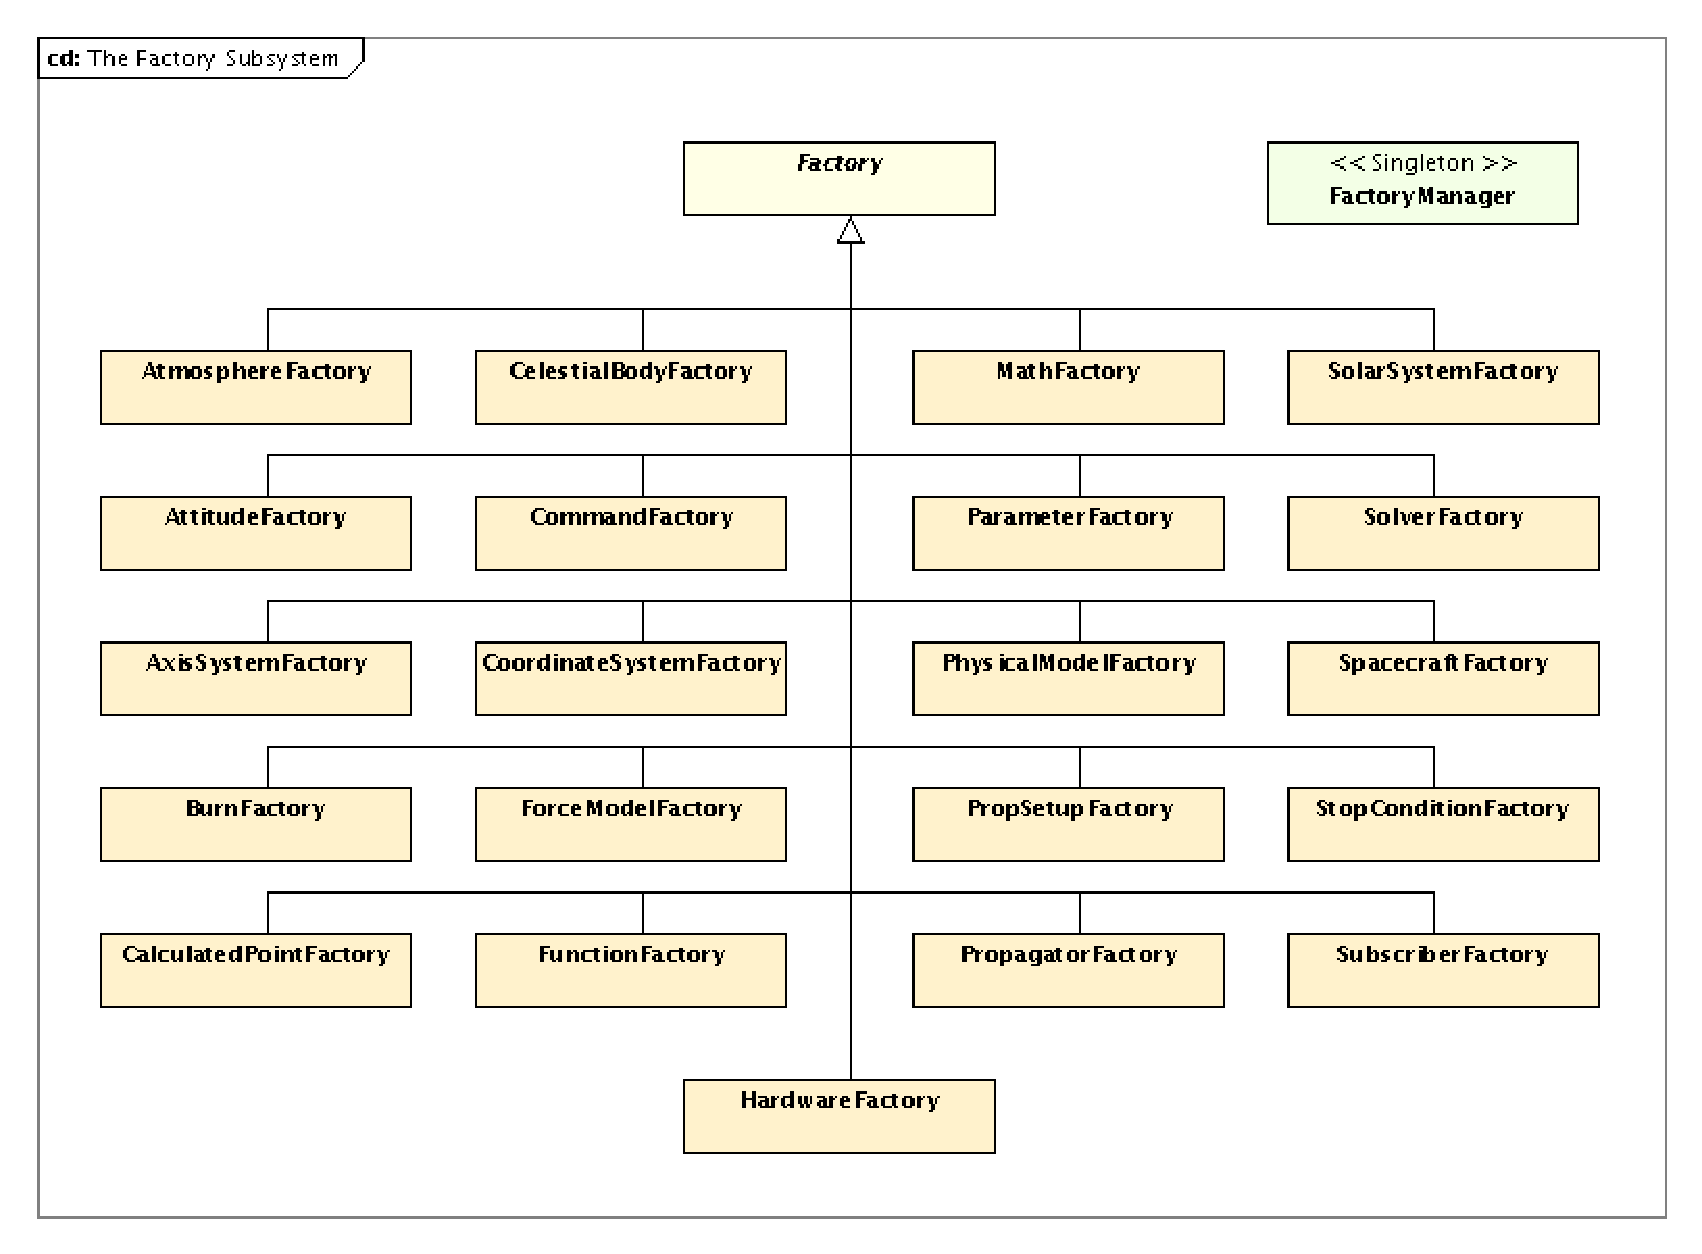
\includegraphics[scale=0.5]{Images/TheFactorySubsystem.eps}
\caption{\label{figure:TheFactorySubsystem}Class Hierarchy for 21 GMAT Factories}
\end{center}
\end{figure}

GMAT contains twenty-one factories at this writing, all implemented in a similar manner to that
shown in the previous section.  These factories are shown in
Figure~\ref{figure:TheFactorySubsystem}.

\subsection{\label{section:UserObjects}Extending GMAT}

Factories are a key element of GMAT's extensibility strategy.  A developer adds a new user component
to GMAT by taking the following steps:

\begin{enumerate}
  \item Design the new component based on GMAT's architecture.
  \item Code the new component, using GmatBase or one of its derivatives as the base class for the
component.
  \item Compile and debug the component as a stand-alone object (as much as possible).
  \item Create a new Factory that creates instances of the new component, or add the component to an
existing Factory\footnote{Factories can support many classes at once; if a convenient Factory
already exists for the developer, the new class can be added to that Factory without any loss of
functionality}.
  \item \label{item:RuntimeRegister}Either build a new shared library that contains the Factory and
the class or classes defining the new component, or incorporate the new classes and Factory in a
GMAT build.
  \item Register the new Factory with the Factory Manager.
  \item Test the new component in GMAT.
  \item Start using the new component.
\end{enumerate}

Note that step~\ref{item:RuntimeRegister} lists two possible ways to build the new code.
Chapter~\ref{chapter:ExtendingGMAT} provides a more thorough introduction to adding new classes to
GMAT, and includes a discussion of registering new components either at runtime or linked in at
compile time.

\begin{figure}[htb]
\begin{center}
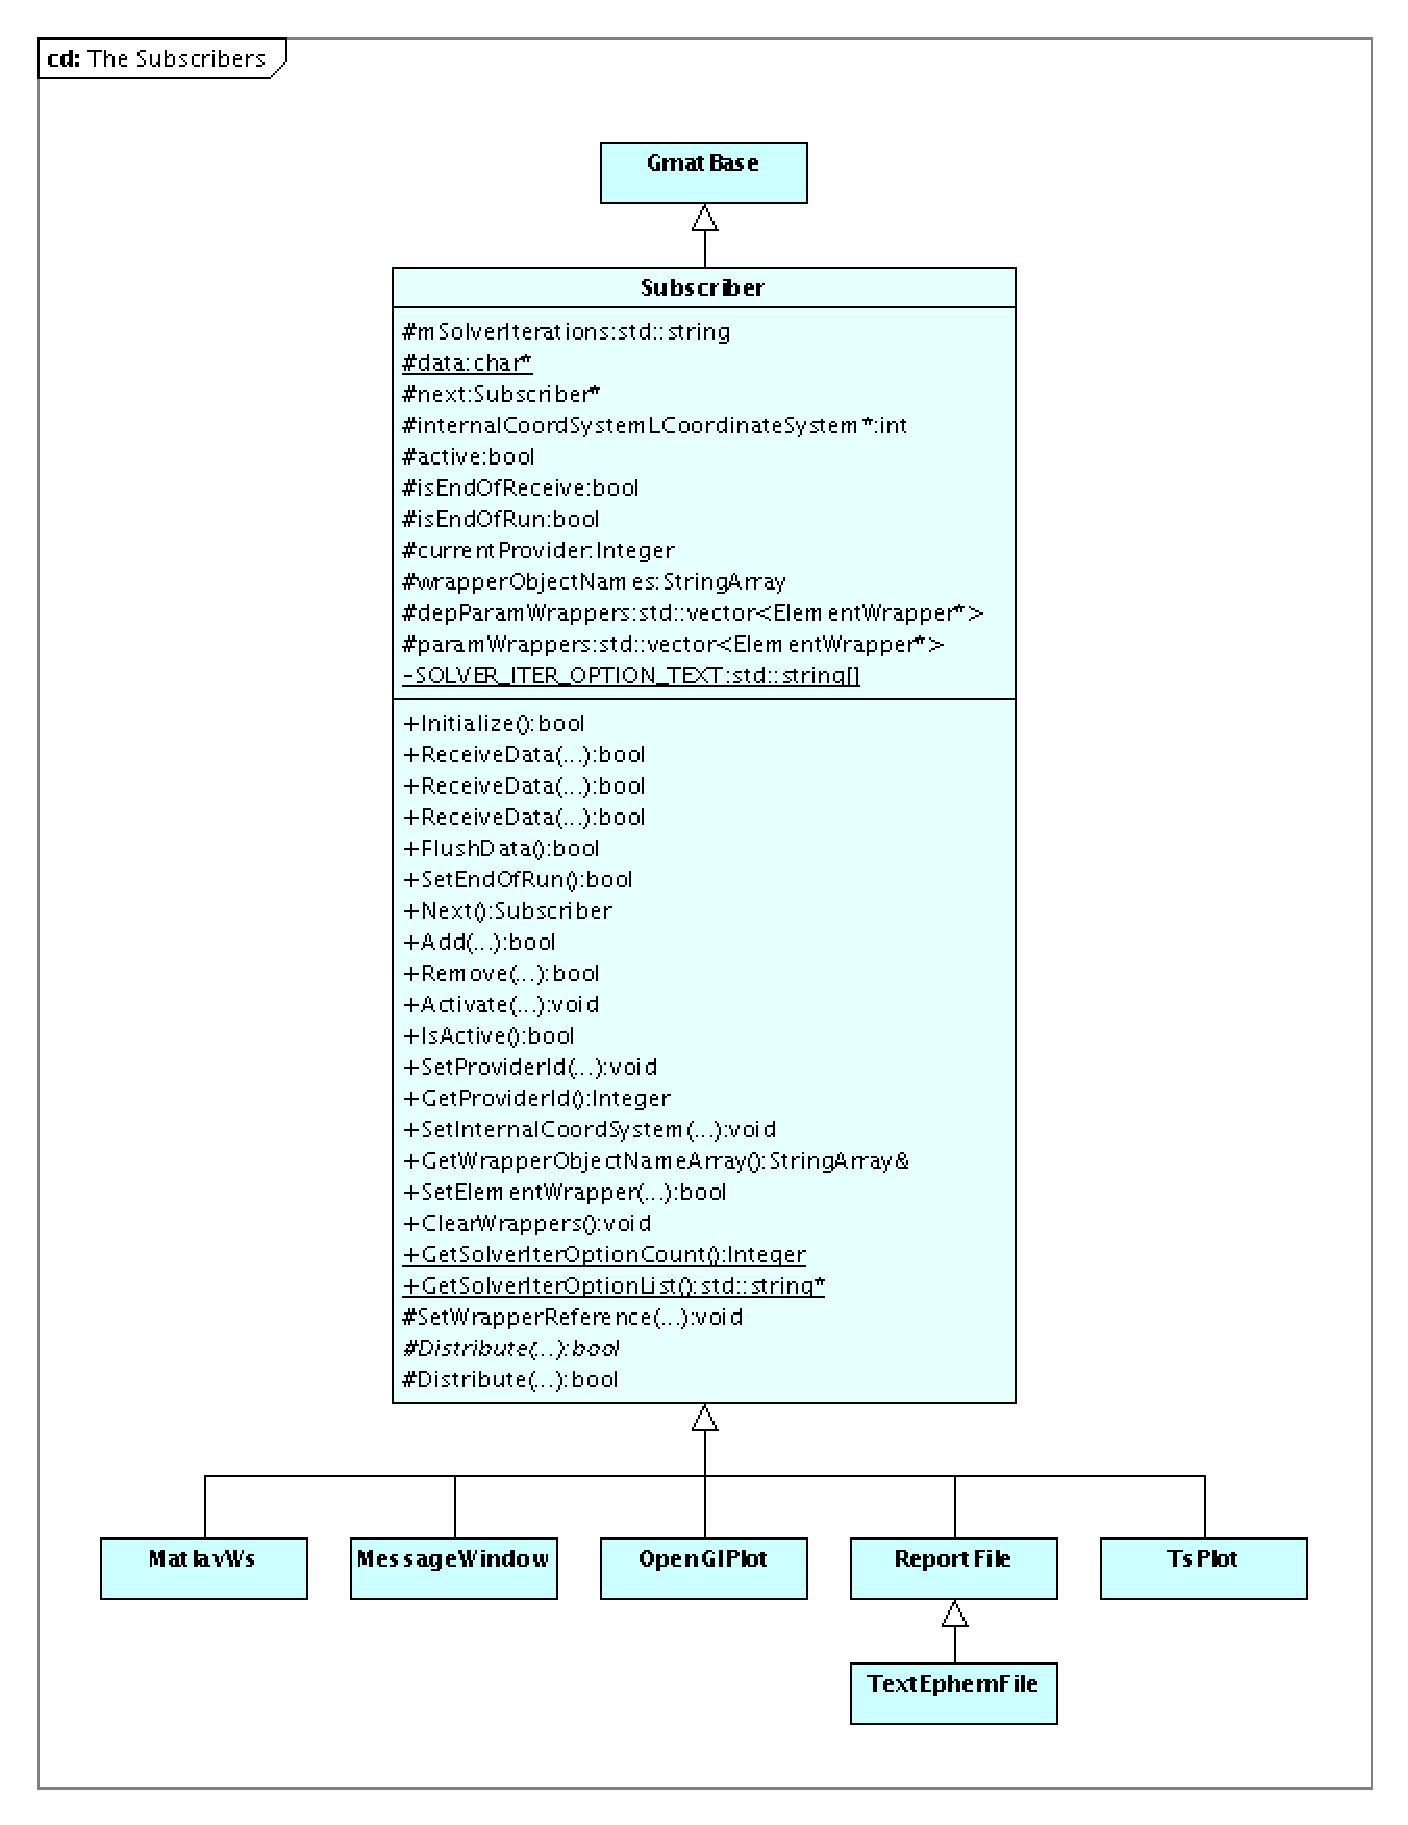
\includegraphics[scale=0.5]{Images/TheSubscribers.eps}
\caption{\label{figure:TheSubscribers}The Subscriber Class}
\end{center}
\end{figure}

\section{Subscribers}

During a Mission Control Sequence run data is sent from the Sandbox to GMAT's Publisher.  The
Publisher routes this data to two and three dimensional plots on the user's display, to report
files, and to any other output objects configured by the user prior to the run.  These output
objects are instances of classes derived from the Subscriber base class, shown in
Figure~\ref{figure:TheSubscribers}.

\subsection{Structure of the Subscribers}

The Subscribers all implement methods and structures designed to work as recipients of the data
delivered from GMAT's Publisher.  These members include several flags used to track the state of a
Mission Control Sequence run, wrappers used for published data, and methods used to pass the data
into the Subscribers and manage Subscriber processing.  The class members are describewd below.

\subparagraph{\textit{Class Attributes}}

\begin{itemize}
\item \textbf{std::string mSolverIterations}: Sets the behavior of the Subscriber when a Solver is
finding a solution.  The current options are ``All'' and ``None''.
\item \textbf{const char *data}: A pointer used in the ReceiveData method to set the input buffer
that is processed.
\item \textbf{CoordinateSystem *internalCoordSystem}: A coordinate system available for conversions
when needed.
\item \textbf{bool active}: Flag specifying if the Subscriber is currently processing data.
\item \textbf{bool isEndOfReceive}: Flag indicating that the current set of data has finished being
sent.
\item \textbf{bool isEndOfRun}: Flag indicating that the current Mission Control Sequence has
finished running.
\item \textbf{Gmat::RunState runstate}: The current run state of the Mission Control Sequence.
\item \textbf{Integer currentProvider}: The ID of the current data privider.
\item \textbf{StringArray wrapperObjectNames}: The list of data wrappers used by the Subscriber.
\item \textbf{std::vector<ElementWrapper*> depParamWrappers}: The data wrappers used for dependent
parameters.
\item \textbf{std::vector<ElementWrapper*> paramWrappers}: The data wrappers used for parameters.
\end{itemize}

\subparagraph{\textit{Methods}}

\begin{itemize}
\item \textbf{virtual bool Initialize()}:  Sets all internal pointers needed to use the Subscriber.
\item \textbf{virtual bool ReceiveData(const char* datastream)}: Receives character data from the
Publisher.  The data passed in is a standard C/C++ string, terminated with a NULL ('\\0')
character.
\item \textbf{virtual bool ReceiveData(const char* datastream, const Integer len)}: Receives
character data from the Publisher.  The data passed in fills a buffer of the indicated length.
\item \textbf{virtual bool ReceiveData(const Real* datastream, const Integer len = 0)}: Receives
Real number data from the Publisher.  The data passed inis in a C/C++ array of the indicated length.
\item \textbf{virtual bool FlushData()}: Method called to tell the Subscriber to process all
received data immediately.
\item \textbf{virtual bool SetEndOfRun()}: Tells the Subscriber that a Mission Control Sequence run
has been complted, so the Subscriber should process all unprocessed data.
\item \textbf{virtual bool SetRunState(Gmat::RunState rs)}: Updates the run state so the subscriber
can act based in state changes.
\item \textbf{void Activate(bool state = true)}: Changes the active flag to the input setting.
Subscribers can use this setting to toggle on or off the processing on input data.
\item \textbf{bool IsActive()}: Returns the value of the active flag.
\item \textbf{virtual void SetProviderId(Integer id)}:
\item \textbf{virtual Integer GetProviderId()}:
\item \textbf{virtual void SetInternalCoordSystem(CoordinateSystem *cs)}:
\item \textbf{virtual const StringArray\& GetWrapperObjectNameArray()}:
\item \textbf{virtual bool SetElementWrapper(ElementWrapper* toWrapper, const std::string \&name)}:
\item \textbf{virtual void ClearWrappers()}: Deletes and sets all wrapper pointers to NULL but
leaves size unchanged.
\item \textbf{static Integer GetSolverIterOptionCount()}:
\item \textbf{static const std::string* GetSolverIterOptionList()}:
\item \textbf{bool SetWrapperReference(GmatBase *obj, const std::string \&name)}:
\item \textbf{virtual bool Distribute(Integer len) = 0}:
\item \textbf{virtual bool Distribute(const Real *dat, Integer len)}:
\end{itemize}

\subparagraph{\textit{Deprecated Attributes and Methods}}

Subscribers were initially prototyped in a linked list structure.  Some artifacts of that design
remain in the current code, but will be removed in a later release.  These pieces are listed below.

\begin{itemize}
\item \textbf{Subscriber *next}: The pointer to the next Subscriber in the list.
\item \textbf{Subscriber* Next()}: Retrieves the next Subscriber for the current list.
\item \textbf{bool Add(Subscriber *s)}: Adds a Subscriber at the end of the list.
\item \textbf{bool Remove(Subscriber *s, const bool del)}: Removes a Subscriber from the list.
\end{itemize}

\subsection{Subscriber Initialization and Execution}

\subsubsection{Defining and Initializing Subscribers}

Each Subscriber in GMAT has an associated GmatBase derived object that is stored in the
configuration and cloned into the Sandbox prior to a run.  These objects are the connection points
between operations occuring in the Sandbox and the data presented to the user, either graphically
or in text form.

\subsubsection{Subscriber Usage During Mission Execution}



% $Id: SolarSystem.tex,v 1.1 2008/01/31 18:04:17 dconway Exp $
\chapter{\label{chapter:SolarSystem}The Space Environment}
\chapauthor{Darrel J. Conway}{Thinking Systems, Inc.}

The core purpose of GMAT is to perform flight dynamics simulations for spacecraft flying in the
solar system.  There are many different components that users interact with to produce this model.
In this chapter, the architecture for the elements that comprise the model is introduced.  The
elements that are not directly manipulated in the model -- specifically, the Sun, planets, moons,
and related points that comprise the stage on which the spacecraft and related objects perform
their actions -- are described in some detail in the chapter.  Descriptions for the other objects
-- most specifically spacecraft and formations -- introduced here appear in chapters for those
components.  References for those chapters are provided when the objects are introduced.

\section{Components of the Model}

The environmental elements that have a spatial location and evolve over time in the GMAT model are
all derived from the SpacePoint class.  The class hierarchy, shown in
Figure~\ref{figure:EnvironmentalObjects}, includes classes that model the objects and
special locations in GMAT's solar system -- referred to as ``background'' objects because their
evolution is modeled through precalculated ephemerides or computations performed off of these
precalculated data -- along with the pieces that are directly manipulated in the mission control
sequence and that evolve through numerical integration using GMAT's propagation subsystem.  In the
figure, the classes used to model background objects are shown in purple; those that evolve through
direct modeling in GMAT using the propagation subsystem are shown in blue, and other elements that
will be incorporated in the future, in red.

\begin{figure}[htb]
\begin{center}
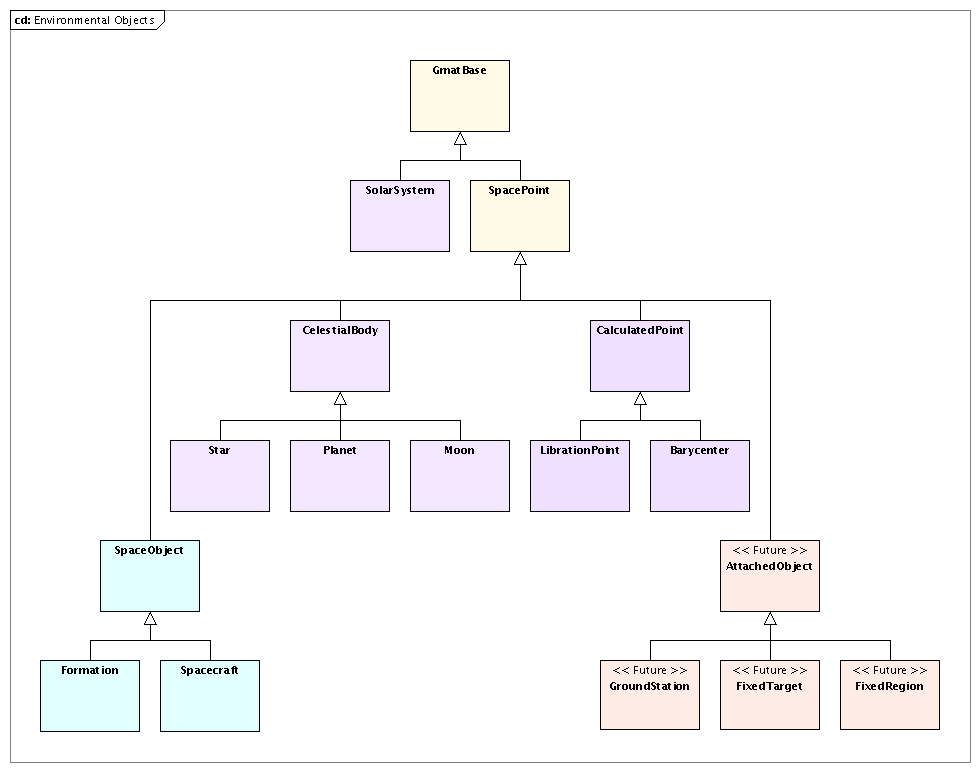
\includegraphics[scale=0.5]{Images/EnvironmentalObjects.eps}
\caption[Objects in the GMAT Model]{\label{figure:EnvironmentalObjects}Objects in the GMAT
Model.\\The elements shown in purple are core constituents of GMAT's solar system.  Classes
shown in yellow are GMAT base classes.  Elements shown in blue are the key components
studied in GMAT's model: Spacecradft and Formations of Spacecraft.  Those shown in red are future
enhancements, primarily focussed on contact analysis with different types of objects.}
\end{center}
\end{figure}

The space environment as defined in this document consists of the elements that, while dynamic, are
automatically updated as the model evolves, based on epoch data generated for the model.  These
elements are the gravitating bodies in the model -- that is, the Sun and the planets and their moons
-- and points with specialized significance in flight dynamics, like the Lagrange points and
gravitational barycenters.  All of these elements are managed in an instance of the SolarSystem
class. SolarSystem acts as a container, and manages both the objects in the space environment and
the resources needed to calculate ephemerides for these objects.  The bulk of this chapter provides
details about the classes and objects comprising this space environment.

A key feature of GMAT is the ability to model spacecraft and formations of spacecraft as they move
through the space environment.  These elements of the model are configured in detail by GMAT users,
and evolve through time using precision numerical integrators configured by the users.  The
Spacecraft and Formation classes, along with their base SpaceObject class, are discussed in detail
in Chapter~\ref{chapter:Spacecraft}.  The numerical integrators and associated force model
components are presented in Chapter~\ref{chapter:Propagators}.

The class hierarchy includes provisions for future model elements attached to components of the
space environment.  These classes, FixedObject and the derived GroundStation, FixedTarget and
FixedRegion classes, will be documented at a later date in preparation for implementation.

Before proceeding with a detailed description of GMAT's space environment, the base class used for
all of the model elements needs some explanation.  Those details are provided in the next section.

\section{\label{section:SpacePoint}The SpacePoint Class}

All spatially modeled components need some common data in order to define the positions of objects
in the model.  These data are collected in the SpacePoint base class.  This base class provides the
foundation for objects used to define coordinate systems (see
Chapter~\ref{chapter:CoordinateSystems}), for the user configured Spacecraft and Formations (see
Chapter~\ref{chapter:Spacecraft}), and for other specialized points and objects in the space
environment.

\begin{figure}[htb]
\begin{center}
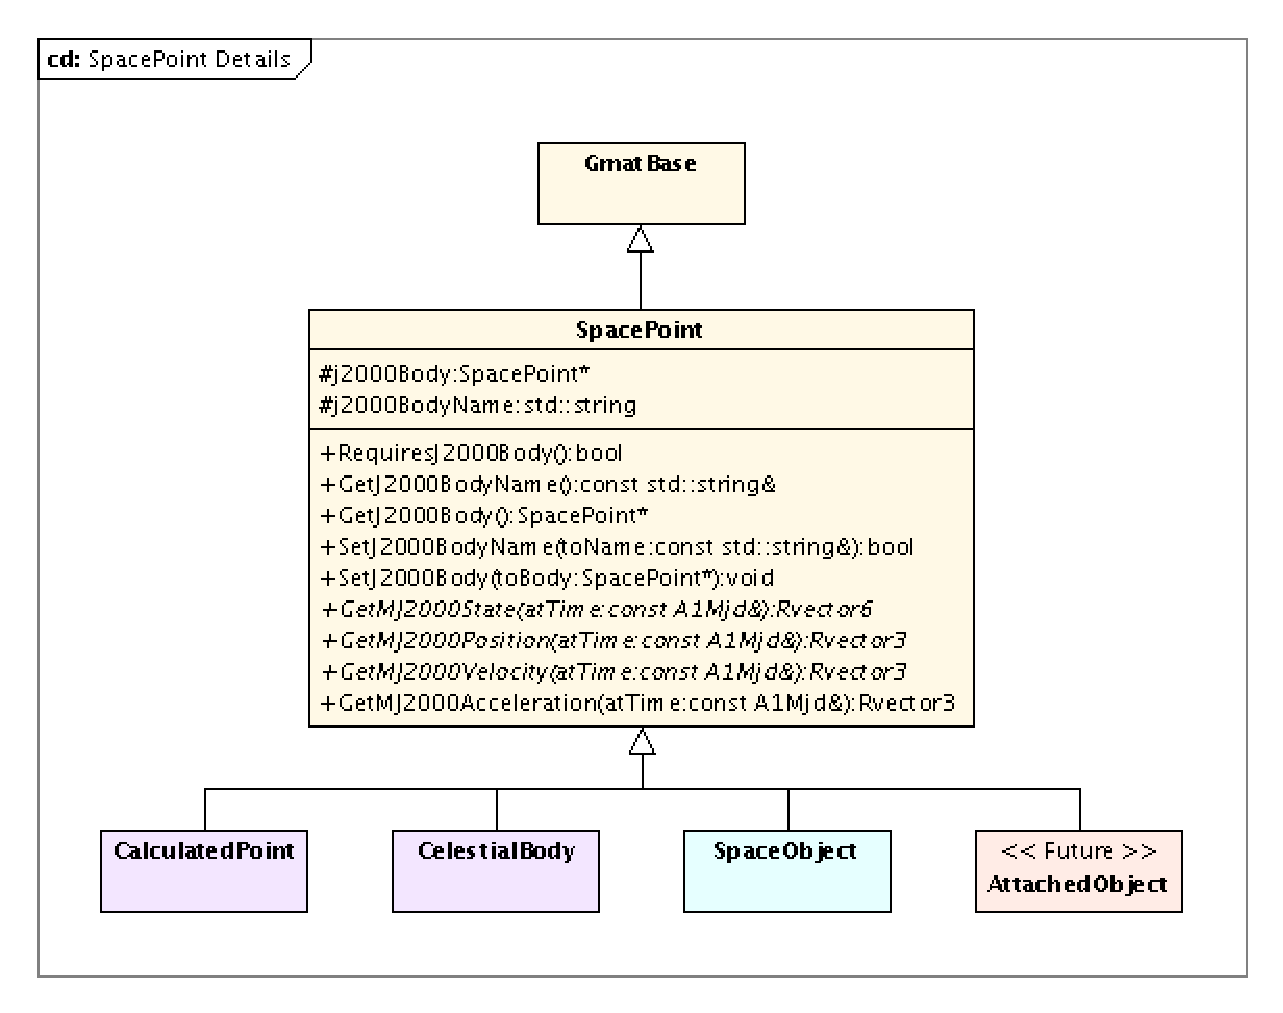
\includegraphics[scale=0.5]{Images/SpacePointDetails.eps}
\caption{\label{figure:SpacePointDetails}The SpacePoint Class}
\end{center}
\end{figure}

Figure~\ref{figure:SpacePointDetails} shows the elements of the SpacePoint class.  In
order for GMAT to accurately model flight dynamics problems, the GMAT space model needs to specify
an internal origin and coordinate system orientation used as a reference for computations.
SpacePoint defines one object, the J2000 body, which is used to define that origin.  GMAT uses the
Mean-of-J2000 Earth Equatorial axis system as the orientation for all such calculations.

\subparagraph{\textit{Class Attributes}}

SpacePoint defines two data members to track the J2000 body:

\begin{itemize}
\item \textbf{SpacePoint* j2000Body}: The body used to define the coordinate origin for the
SpacePoint.
\item \textbf{std::string j2000BodyName}: The name of the body defining the coordinate origin.
\end{itemize}

\subparagraph{\textit{Methods}}

All classes derived from SpacePoint inherit the implementation of six methods used to set and access
the J2000 body.  Five of these methods are used specifically for the internal data members; the
sixth, GetMJ2000Acceleration(), provides a default implementation so that derived classes that do
not have acceleration data do not need to provide an implementation

\begin{itemize}
\item \textbf{bool RequiresJ2000Body()}: Returns a boolean used to determine if the SpacePoint
requires a J2000 body.
\item \textbf{const std::string\& GetJ2000BodyName()}: Returns the name of the J2000 body for the
SpacePoint.
\item \textbf{SpacePoint *GetJ2000Body()}: Returns the pointer to the J2000 body for the
SpacePoint.
\item \textbf{bool SetJ2000BodyName(const std::string \&toName)}: Sets the name of the J2000 body
for the SpacePoint.
\item \textbf{void SetJ2000Body(SpacePoint *toBody)}: Sets the pointer to the J2000 body for the
SpacePoint.
\item \textbf{Rvector3 GetMJ2000Acceleration(const A1Mjd \&atTime)}: Returns the Cartesian
acceleration of the SpacePoint relative to its J2000 body at the specified epoch.  The default
implementation returns [0.0, 0.0, 0.0]; derived classes that contain acceleration data should
override this method.
\end{itemize}

\subparagraph{\textit{Abstract Methods}}

Each subclass of SpacePoint implements three pure virtual methods defined in the class, using
computations specific to that subclass.  THese abstract methods have the following signatures:

\begin{itemize}
\item \textbf{virtual Rvector6 GetMJ2000State(const A1Mjd \&atTime) = 0}: Returns the Cartesian
state of the SpacePoint relative to its J2000 body at the specified epoch.
\item \textbf{virtual Rvector3 GetMJ2000Position(const A1Mjd \&atTime) = 0}: Returns the Cartesian
location of the SpacePoint relative to its J2000 body at the specified epoch.
\item \textbf{virtual Rvector3 GetMJ2000Velocity(const A1Mjd \&atTime) = 0}: Returns the Cartesian
velocity of the SpacePoint relative to its J2000 body at the specified epoch.
\end{itemize}

\section{The Solar System Elements}

GMAT provides a container class, SolarSystem, that is used to manage the objects modeling the space
environment.

\subsection{The SolarSystem Class}

\subsubsection{Members and Methods}

\subsubsection{Ephemeris Sources}

\subsection{The CelestialBody Class Hierarchy}

\subsubsection{Stars}

\subsubsection{Planets}

\subsubsection{Moons}

\section{The PlanetaryEphem Class}



% $Id: CoordinateSystems.tex,v 1.1 2008/01/31 18:04:16 dconway Exp $
\chapter{\label{chapter:CoordinateSystems}Coordinate Systems}
\chapauthor{Darrel J. Conway}{Thinking Systems, Inc.}

\textbf{NOTE: This chapter currently contains the original design spec for the coordinate systems.
It needs to be reviewed against the current GMAT system, the figures need to be recreated, and some
of the text needs to be fitted into the rest of the design document.}

This chapter presents design guidelines for the coordinate system classes in the Goddard Mission
Analysis Tool (GMAT). It describes how the GMAT software implements the coordinate system math
described in the GMAT Mathematical Specifications\cite{mathSpec}. This description includes the
initial design for the classes that provide coordinate system support in GMAT. The interactions
between these classes and the rest of the GMAT system are also described.

\section{Introduction}

The Goddard Mission Analysis Tool (GMAT) is a multi-platform orbit simulator designed to support
multiple spacecraft missions flying anywhere in the solar system. GMAT is written in C++ and runs on
Windows, Macintosh and Linux computer systems. The tool provides an integrated interface to MATLAB,
a high level computing environment from the Mathworks, Inc\cite{MATLAB}. The GMAT graphical user
interface (GUI) is written using the wxWidgets GUI Toolkit\cite{wxWidgets}, an open source library
that compiles and runs under all of the target operating systems.

GMAT is an object-oriented system, using the full extent of the C++ language to implement the object
model that provides GMAT's functionality.  The first three builds of GMAT provided capabilities to
model orbits in the vicinity of the Earth, including detailed force modeling, impulsive
maneuvers, and parameter targeting using a differential corrector.  All of these capabilities can be
controlled either using either the GMAT graphical user interface or a custom scripting language
designed to simplify GMAT and MATLAB interactions. The fourth build of the system generalizes the
capabilities of GMAT modeling for other orbital regimes.

In order to model spacecraft trajectories in these regimes, GMAT needs to be able to represent the
spacecraft state and related quantities in coordinate systems that are convenient to each regime.
This document describes how these coordinate systems are implemented in the GMAT code.


\section{\label{sec:CSClassDescription}Coordinate System Classes}

Figure \ref{figure:HighLevelCSClasses} shows the core C++ classes (drawn using
Poseidon\cite{poseidon}) added to GMAT to provide support for coordinate systems in Build 4. The
coordinate system capabilities are provided by the incorporation of these classes into the GMAT base
subsystem\footnote{The GMAT code base consists of a set of classes that provide the core
functionality of the system, the {}``base'' subsystem, and classes that comprise the graphical user
interface, the {}``gui'' subsystem.  All of the classes described in this document are members of
the base subsystem, with the exception of the recommendations for changes to the panels on the
GUI.}.

\begin{figure}[htb]
\begin{center}
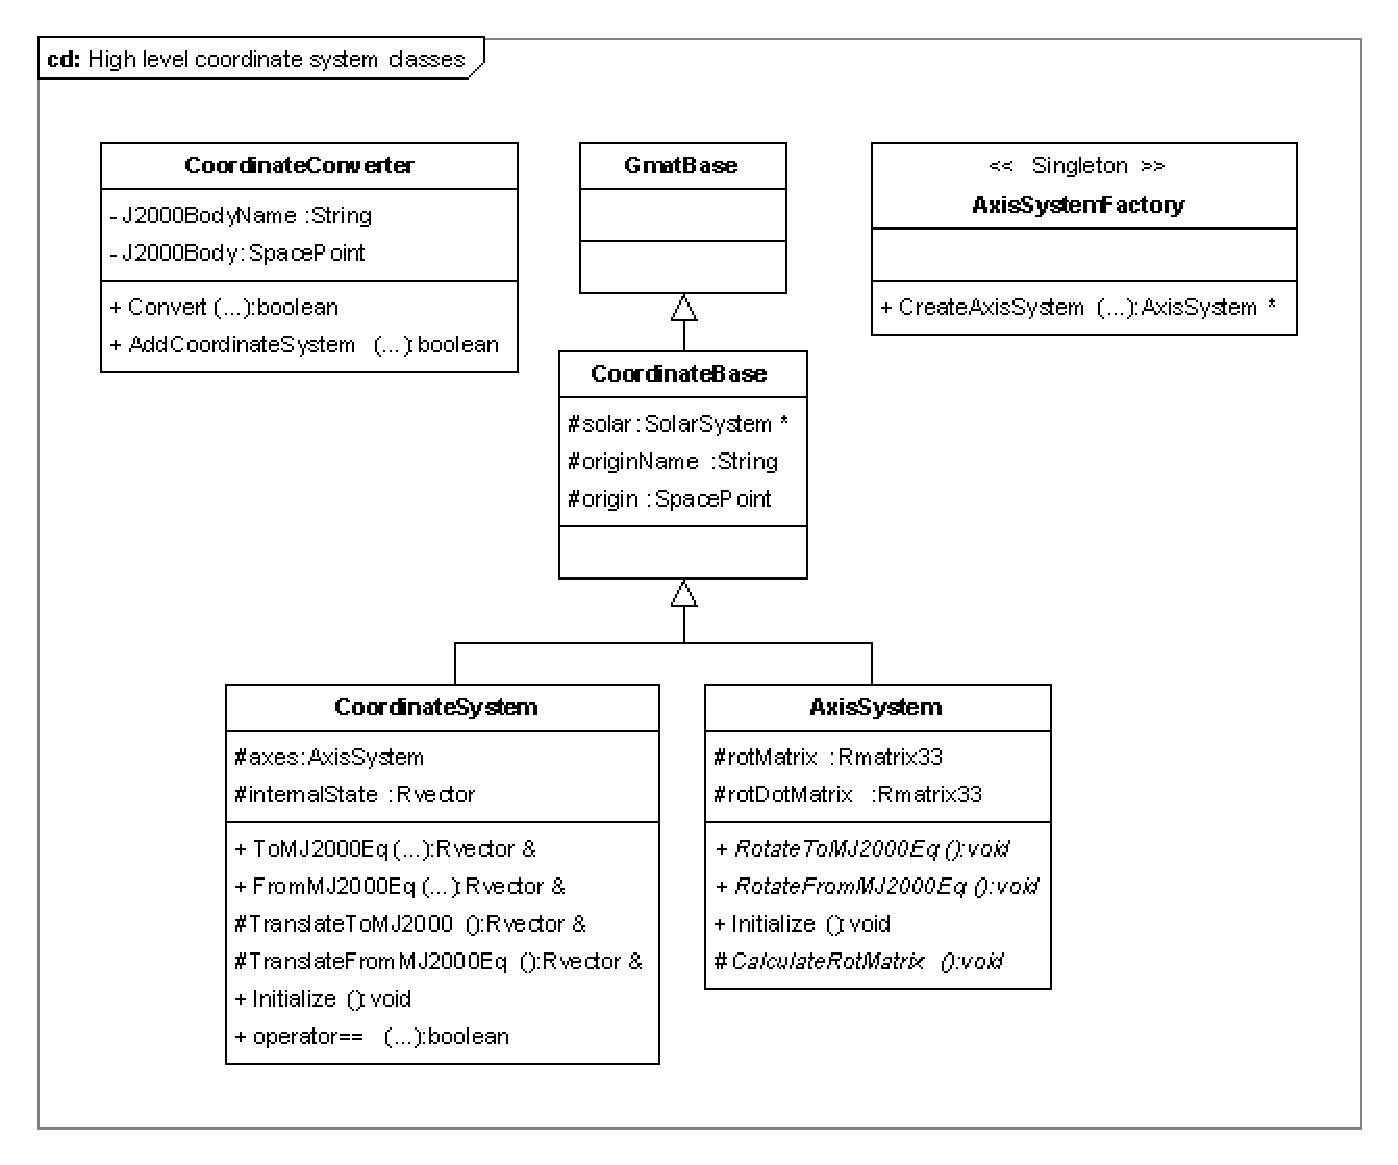
\includegraphics[scale=0.5]{Images/Highlevelcoordinatesystemclasses.eps}
\caption{\label{figure:HighLevelCSClasses}Coordinate System Classes in GMAT}
\end{center}
\end{figure}

The coordinate system classes consist of a CoordinateSystem class that acts as the interface between
the conversions and the rest of GMAT, an AxisSystem base class with a derived hierarchy used for
rotational conversions, a CoordinateConverter class that manages conversions between different
coordinate systems, and a factory constructed as a singleton that create the AxisSystem objects. The
CoordinateSystem class is the component that is instantiated when a user {}``Creates'' a coordinate
system object.

Previous builds of GMAT included classes that model spacecraft, formations, and celestial objects.
These classes were derived from a core base class named GmatBase. A new intermediate class,
SpacePoint, is implemented in GMAT to make access to position, velocity, and rotational data
available to the coordinate system classes when needed. Section~\ref{sub:SpacePointClassDescription}
describes this class.


\subsection{The CoordinateSystem Class}

The CoordinateSystem class is a configured component that implements the functionality needed to
convert into and out of a specified coordinate system. Internally, GMAT performs computations in a
Mean of J2000 Earth Equatorial coordinate system, centered at one of the celestial bodies in the
GMAT solar system (i.e. the Sun, a planet, or a moon) or at a barycenter or libration point. Each
CoordinateSystem instance provides methods to transform into and out of these J2000 coordinate
systems. It contains the data necessary for translation calculations, along with a member object
pointer that is set to an AxisSystem instance for coordinate systems whose principle axes are not
parallel to the Mean of J2000 Earth Equatorial axes, or to NULL for coordinate systems that are
oriented parallel to these axes.

The AxisSystem class provides the methods needed to rotate the coordinate system into and out of the
Mean of J2000 Earth Equator frame.  The AxisSystem is set for a given CoordinateSystem by setting
the axes member to an AxisSystem instance.

GMAT uses a late binding scheme to provide interconnections between objects used when modeling an
analysis problem. Individual components are configured from either the grapical user interface or a
script file describing the objects that need to be modeled. Connections between these objects are
defined using the names of the objects, but the actual object instances used in the model are not
set until the simulation is run. Upon execution, the configured objects are copied into the analysis
workspace, called the Sandbox, and the connections between the configured objects are established
immediately prior to the run of the simulation. The Initialize method in the CoordinateSystem class
implements this late binding for the connection between the coordinate system instance and the
related SpacePoints.


\subsection{The AxisSystem Class Hierarchy}

GMAT is capable of supporting numerous coordinate system orientations.  These orientations are
defined through the AxisSystem class; each unique axis orientation is implemented as a separate
class derived from the AxisSystem base class. Figure~\ref{figure:AxisSystemOverview} shows an
overview of the AxisSystem class hierarchy, and identifies the top level classes in this hierarchy.

\begin{figure}
\begin{center}
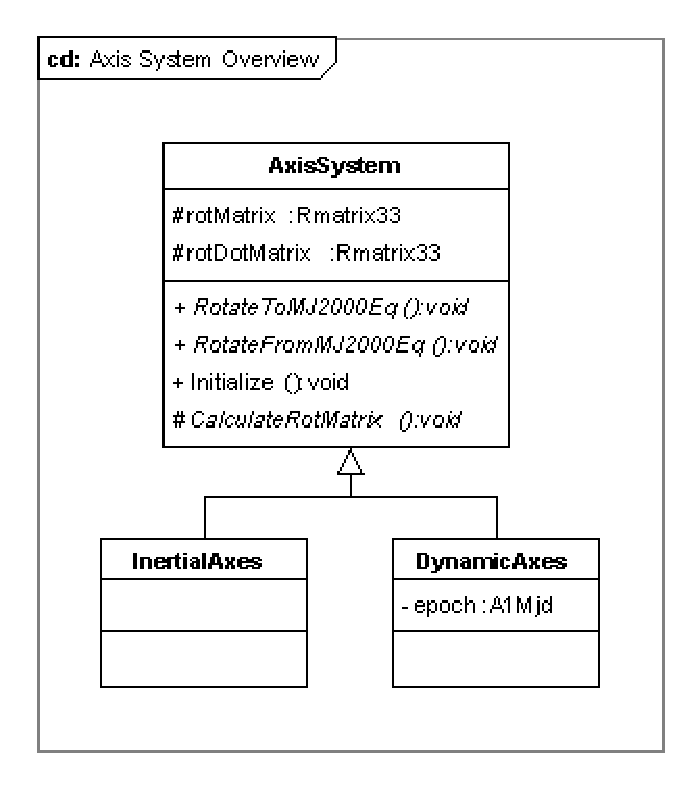
\includegraphics[scale=0.5]{Images/AxisSystemOverview.eps}
\caption{\label{figure:AxisSystemOverview}Top level AxisSystem Derived Classes}
\end{center}
\end{figure}

The orientations of the coordinate systems in GMAT fall into two broad categories: axes that change
orientation over time, and those that remain fixed in orientation. The latter category requires
computation of the rotation matrices one time, at initialization, in order to perform the rotations
into and out of the coordinate system.  Figure~\ref{figure:InertialAxisHierarchy} shows the six
inertial axis systems supported in GMAT. These systems support equatorial and ecliptic versions
of Mean of J2000, Mean of Epoch, and True of Epoch transformations.

\begin{figure}
\begin{center}
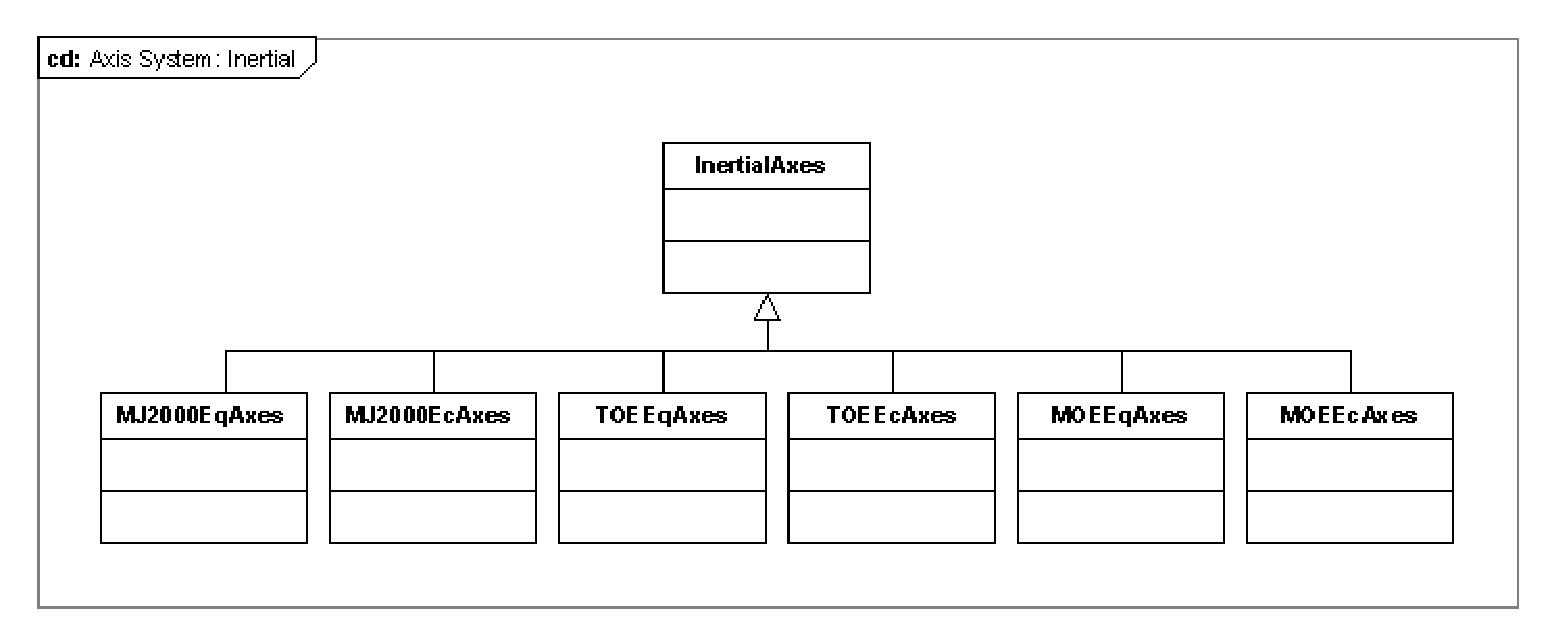
\includegraphics[scale=0.5]{Images/AxisSystemInertial.eps}
\caption{\label{figure:InertialAxisHierarchy}Inertial Axis Classes}
\end{center}
\end{figure}

Coordinate systems that are not fixed in orientation over time are derived from the DynamicAxes
class, as is shown in Figure~\ref{figure:DynamicAxisHierarchy}.  These coordinate systems include
equatorial and ecliptic versions of the mean of date and true of date axes, along with axes that
evolve with the polar motion of the body's rotational axis (implemented in the EquatorAxes class)
and axes that are fixed on the body's prime meridian (the BodyFixedAxes class). All of these classes
require recomputation of the orientation of the axes as the epoch of the model evolves.

\begin{figure}
\begin{center}
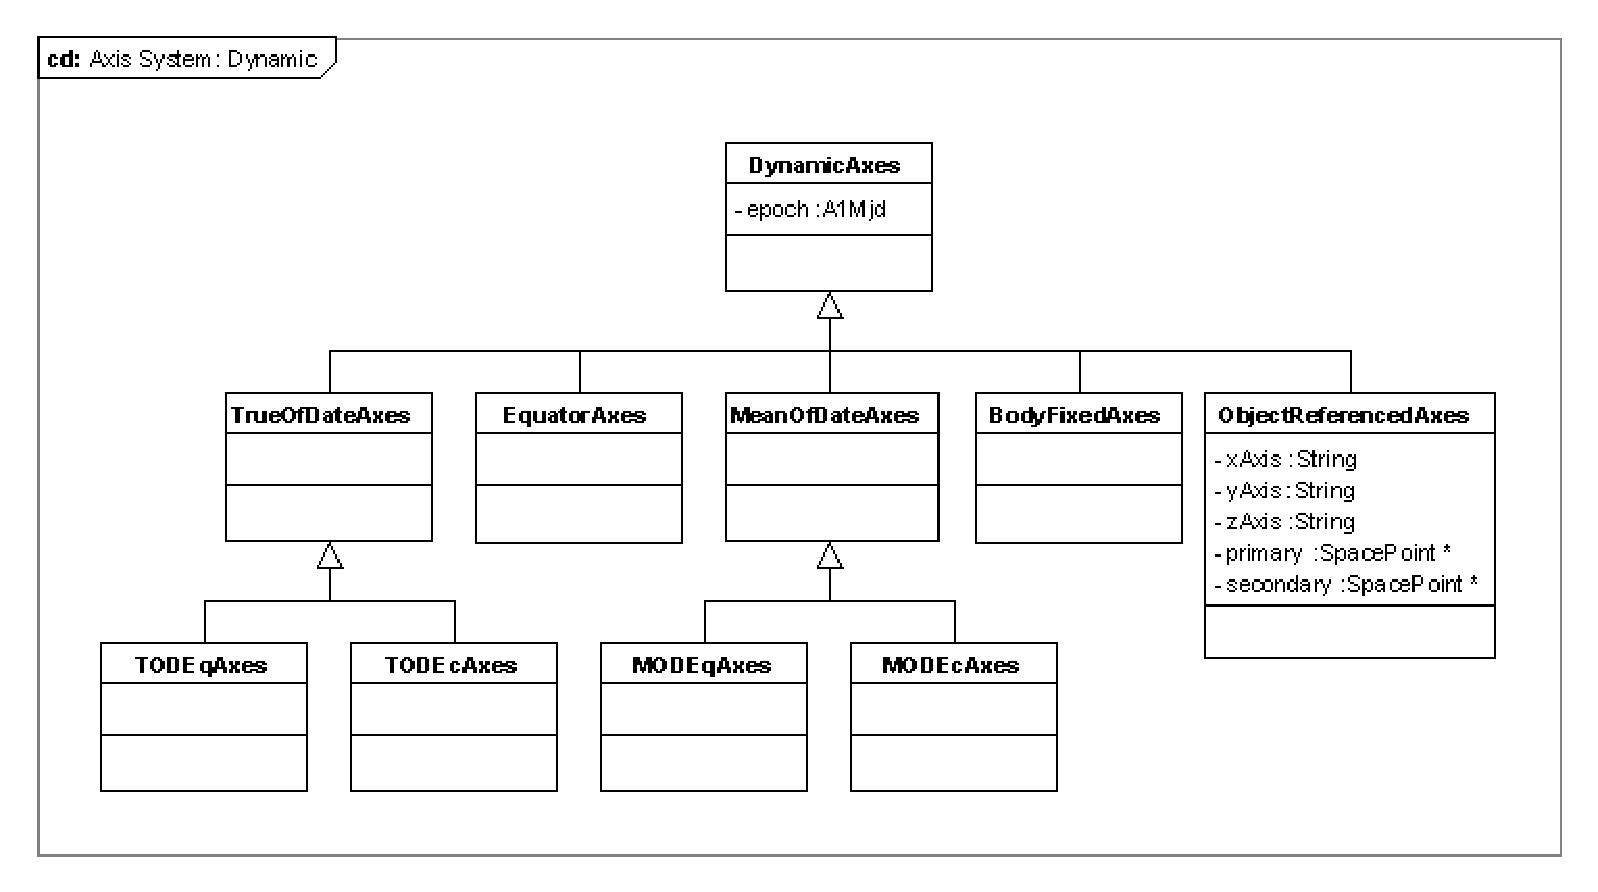
\includegraphics[scale=0.5]{Images/AxisSystemDynamic.eps}
\caption{\label{figure:DynamicAxisHierarchy}Dynamic Axis Classes}
\end{center}
\end{figure}

One additional class in Figure~\ref{figure:DynamicAxisHierarchy} bears discussion here. GMAT
supports numerous coordinate systems that reference bodies that are not celestial objects --
specifically coordinate systems that use Lagrange points, barycenters, spacecraft, and formations to
define the coordinate origins and axes. These coordinate systems use the ObjectReferencedAxes class
to construct the coordinate basis and rotation matrices. The GMAT Mathematical
Specifications\cite{mathSpec} provide detailed descriptions of how this class operates.

\subsection{CoordinateSystem and AxisSystem Collaboration}

The GMAT Mathematical Specification\cite{mathSpec} includes a flow chart that describes the
process of transforming between coordinate systems. This process is performed in the GMAT code using
the CoordinateConverter class and the public methods of the CoordinateSystem class. When GMAT needs
a conversion from one coordinate system to another, the method \texttt{CoordinateConverter::Convert}
is called with the epoch, input state, input coordinate system, output state, and output coordinate
system as parameters. The converted state vector is stored in the output state parameter.

The Convert method calls the conversion method \texttt{CoordinateSystem::ToMJ2000Eq} on the input
coordinate system, followed by \texttt{CoordinateSystem::FromMJ2000Eq} on the output coordinate
system. \texttt{ToMJ2000Eq} calls the \texttt{AxisSystem::RotateToMJ2000Eq} method followed by the
\texttt{Coordinate\-System::TranslateToMJ2000Eq} method, converting the input state from the input
coordinate system into Mean of J2000 Equatorial coordinates. Similarly, \texttt{FromMJ2000Eq} calls
the \texttt{Coordinate\-System::TranslateFromMJ2000Eq} method and then the
\texttt{AxisSystem::RotateFromMJ2000Eq} method, converting the intermediate state from Mean of J2000
Equatorial coordinates into the output coordinate system, completing the transformation from the
input coordinate system to the output coordinate system. Each of the conversion routines takes a
SpacePoint pointer as the last parameter in the call. This parameter identifies the J2000 coordinate
system origin to the conversion routine. If the pointer is NULL, the origin is set to the Earth.

The following paragraphs provide programmatic samples of these conversions.

\subsubsection{Code Snippets for a Conversion}

Figure~\ref{figure:TransformDetails}, generalized from the GMAT mathematical
specification, illustrates the procedure used to implement a transformation
from one coordinate system to another. The following paragraphs provide
code snippets with the corresponding function arguments for this process.

\begin{figure}
\begin{center}
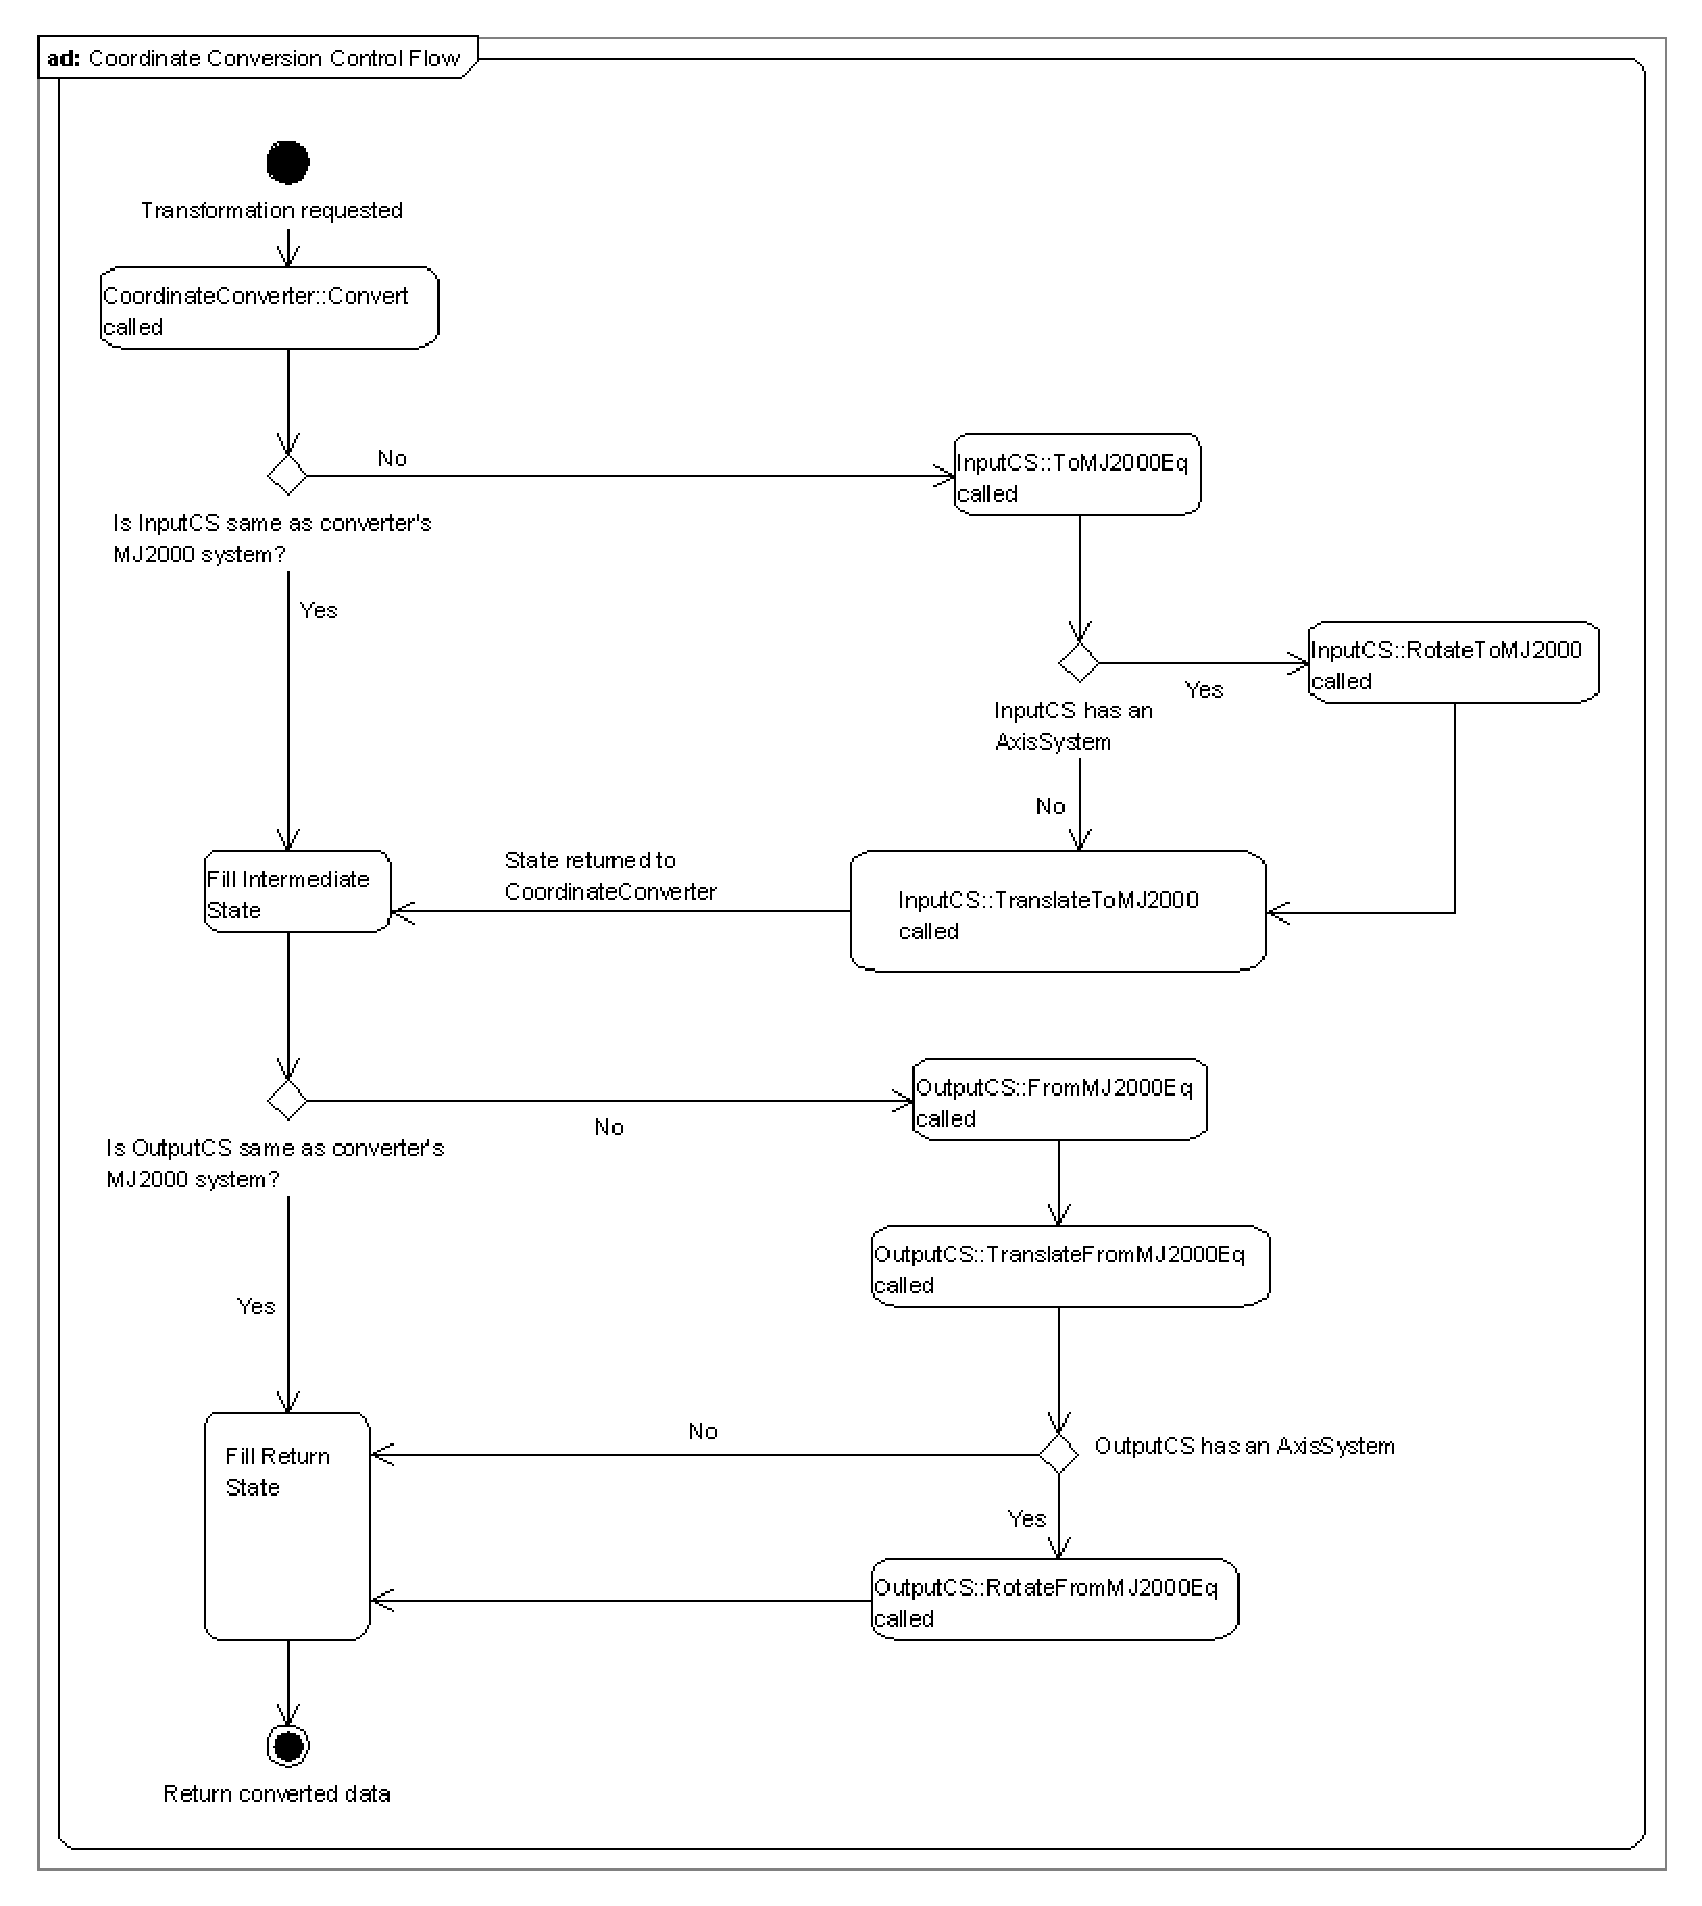
\includegraphics[scale=0.5]{Images/CoordinateConversionControlFlow.eps}
\caption{\label{figure:TransformDetails}GMAT Procedure for a Generic Coordinate Transformation}
\end{center}
\end{figure}

When GMAT needs to convert from one coordinate system to another, this method is called:

\begin{quotation}
\begin{verbatim}
if (!coordCvt->Convert(epoch, instate, inputCS, outstate, outputCS))
   throw CoordinateSystemException("Conversion from " +
      inputCS->GetName() + " to " + outputCS->GetName() + " failed.");
\end{verbatim}
\end{quotation}

This method invokes the calls listed above, like this:

\begin{quotation}
\begin{verbatim}
// Code in CoordinateConverter::Convert
if (!inputCS->ToMJ2000Eq(epoch, instate, internalState, J2000Body))
   throw CoordinateSystemException("Conversion to MJ2000 failed for " +
      inputCS->GetName());

if (!outputCS->FromMJ2000Eq(epoch, internalState, outState, J2000Body))
   throw CoordinateSystemException("Conversion from MJ2000 failed for " +
      outputCS->GetName());
\end{verbatim}
\end{quotation}

The conversion code from the input state to Mean of J2000 Equatorial
Coordinates is accomplished using the calls

\begin{quotation}
\begin{verbatim}
// Code in CoordinateSystem::ToMJ2000Eq
if (axes)      // axes == NULL for MJ2000Eq orientations
   if (!axes->RotateToMJ2000Eq(epoch, instate, internalState, J2000Body))
      throw CoordinateSystemException("Rotation to MJ2000 failed for " +
         instanceName);
else           // Set the intermediate state to the input state
   internalState = instate;

if (!TranslateToMJ2000Eq(epoch, internalstate, internalState, J2000Body))
   throw CoordinateSystemException("Translation to MJ2000 failed for " +
      instanceName);
\end{verbatim}
\end{quotation}

and the conversion from Mean of J2000 Equatorial Coordinates to the output state is performed using
these calls:

\begin{quotation}
\begin{verbatim}
// Code in CoordinateSystem::FromMJ2000Eq
if (!TranslateFromMJ2000Eq(epoch, internalstate, internalState, J2000Body))
   throw CoordinateSystemException("Translation from MJ2000 failed for " +
      instanceName);

if (axes)      // axes == NULL for MJ2000Eq orientations
   if (!axes->RotateFromMJ2000Eq(epoch, internalState, outstate, J2000Body))
      throw CoordinateSystemException("Rotation from MJ2000 failed for " +
         instanceName);
else           // Set the output state to the intermediate state
   outstate = internalState;
\end{verbatim}
\end{quotation}

\subsection{\label{sub:SpacePointClassDescription}The SpacePoint Class}

In general, coordinate systems are defined in reference to locations and directions in space. Many
of the coordinate systems used in GMAT have the direction fixed based on an external reference --
for example, the MJ2000Eq system has the z-axis pointed along the Earth's rotation axis at the J2000
epoch and the x-axis aligned with the vernal equinox at the same epoch. GMAT also supports
coordinate systems constructed in reference to objects internal to the GMAT -- typically a planet,
the Sun, a moon, or a spacecraft can be used, as can special points in space like Lagrange points or
the barycenter of a multi-body system.  The coordinate system classes need to be able to access
position and velocity data about these objects in a generic fashion. GMAT has a class, SpacePoint,
that provides this access. SpacePoint is the base class for all of the objects that model location
data in the solar system, as is shown in Figure~\ref{figure:SpacePointHierarchy}.  The SpacePoint
class is described in more detail in Chapter~\ref{chapter:SolarSystem}.

\begin{figure}
\begin{center}
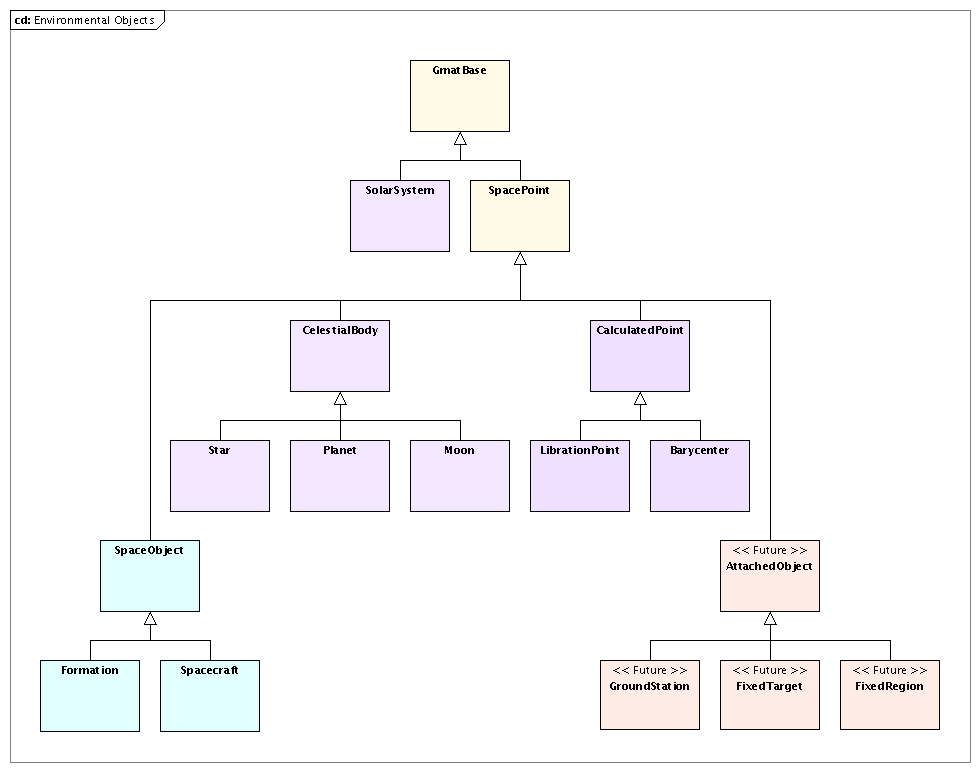
\includegraphics[scale=0.5]{Images/EnvironmentalObjects.eps}
\caption{\label{figure:SpacePointHierarchy}The SpacePoint Class Hierarchy}
\end{center}
\end{figure}

\section{\label{sec:CSScriptConfiguration}Configuring Coordinate Systems}

\subsection{Scripting a Coordinate System}

The script commands used to create a coordinate system object in GMAT are defined in the GMAT
Mathematical Specifications\cite{mathSpec}.  Coordinate System scripting is performed using the
following lines of script:

\begin{quotation}
\begin{verbatim}
Create CoordinateSystem csName
GMAT csName.Origin = <SpacePoint name>;
GMAT csName.Axes = <Axis type>;
GMAT csName.Primary = <Primary SpacePoint name, if needed>;
GMAT csName.Secondary = <Secondary SpacePoint name, if needed>;
GMAT csName.Epoch.<Format> = <Epoch data, if needed>;

% Only two of these three can exist for a given coordinate system;
% see the coordinate system table for more information
GMAT csName.XAxis = <$\pm$R, $\pm$V, or $\pm$N>;
GMAT csName.YAxis = <$\pm$R, $\pm$V, or $\pm$N>;
GMAT csName.ZAxis = <$\pm$R, $\pm$V, or $\pm$N>;
\end{verbatim}
\end{quotation}

The fields in angle brackets are used to set the parameters that define the coordinate system.
Table~\ref{table:CSParms} provides a brief description of these fields; more details are available
in \cite{mathSpec}.

%
\begin{table}
\caption{\label{table:CSParms}Coordinate System Parameters}
\begin{center}\begin{tabular}{|p{0.8in}|p{0.9in}|p{1.3in}|p{2.5in}|}
\hline
Parameter&
Required/ Optional&
Allowed Values&
Description\tabularnewline
\hline
\hline
Origin&
Required&
\begin{flushleft}Any Named SpacePoint\end{flushleft}&
Defines the location of the coordinate system origin.\tabularnewline
\hline
Axes&
Required&
\begin{flushleft}Equator, MJ2000Ec, MJ2000Eq, TOEEq, MOEEq, TODEq,
MODEq, TOEEc, MOEEc, TODEc, MODEc, Fixed, ObjectRefernced\end{flushleft}&
Defines the orientation of the coordinate axes in space.\tabularnewline
\hline
Primary&
Optional&
\begin{flushleft}Any Named SpacePoint\end{flushleft}&
Defines the primary body used to orient axes for systems that need
a primary body.\tabularnewline
\hline
Secondary&
Optional&
\begin{flushleft}Any Named SpacePoint\end{flushleft}&
Defines the secondary body used to orient axes for systems that need
a secondary body.\tabularnewline
\hline
Epoch&
Optional&
Any GMAT Epoch&
Sets the reference epoch for systems that need a reference epoch.\tabularnewline
\hline
XAxis&
Optional&
$\pm\textrm{R,}\pm\textrm{V,}\pm\textrm{N}$&
Used for ObjectReferences axes only; two of the three axes are set,
and one must reference $\pm N$.\tabularnewline
\hline
YAxis&
Optional&
$\pm\textrm{R,}\pm\textrm{V,}\pm\textrm{N}$&
Used for ObjectReferences axes only; two of the three axes are set,
and one must reference $\pm N$.\tabularnewline
\hline
ZAxis&
Optional&
$\pm\textrm{R,}\pm\textrm{V,}\pm\textrm{N}$&
Used for ObjectReferences axes only; two of the three axes are set,
and one must reference $\pm N$.\tabularnewline
\hline
\end{tabular}\end{center}
\end{table}

In the following paragraphs, the interactions between the script interpreter subsystem and the
coordinate system classes are described.

\subsubsection{Script Interpreter Actions}

In GMAT, the ScriptInterpreter reads each line of script and sets up the corresponding objects. The
lines of script above map to calls made in the ScriptInterpreter code, as described in the following
text.

The Create line causes the ScriptInterpreter to call the CoordinateSystemFactory and requests a
CoordinateSystem instance:

\begin{quotation}
\begin{verbatim}
// In the Interpreter subsystem
GmatBase *csInstance = moderator->CreateCoordinateSystem("CoordinateSystem", "csName");
\end{verbatim}
\end{quotation}

The resulting coordinate system is registered with the configuration manager.

The Origin line sets the originName parameter on this instance:

\begin{quotation}
\begin{verbatim}
// First determine that the parm is a string
Gmat::ParameterType type = csInstance->GetParameterType({}``Origin'');

// Here type is a string, so this is called:
csInstance->SetStringParameter({}``Origin'', <SpacePoint name>);
\end{verbatim}
\end{quotation}

The Axes line creates an instance of the AxisSystem and passes it to the coordinate system:

\begin{quotation}
\begin{verbatim}
// First determine that the parm is an internal object
Gmat::ParameterType type = csInstance->GetParameterType({}``Axes'');

// Here type is an object, so this is called:
GmatBase {*}axesInstance = moderator->CreateAxisSystem(<Axis type>, {}``'');

// Then the object is set on the coordinate system
csInstance->SetRefObject(axesInstance);
\end{verbatim}
\end{quotation}

The Primary line sets the primary body on the AxisSystem instance.  This is done by passing the data
through the CoordinateSystem object into the AxisSystem object:

\begin{quotation}
\begin{verbatim}
// First determine that the parm is a string
Gmat::ParameterType type = csInstance->GetParameterType({}``Primary'');

// Pass the string to the coordinate system
csInstance->SetStringParameter({}``Primary'', <SpacePoint name>);

...

// In CoordinateSystem, this parameter is passed to the AxisSystem:
axes->SetStringParameter({}``Primary'', <SpacePoint name>);
\end{verbatim}
\end{quotation}

The Secondary line is treated similarly to the primary line:

\begin{quotation}
\begin{verbatim}
// First determine that the parm is a string
Gmat::ParameterType type = csInstance->GetParameterType({}``Secondary'');

// Pass the string to the coordinate system
csInstance->SetStringParameter({}``Secondary'', <SpacePoint name>);

...

// In CoordinateSystem, this parameter is passed to the AxisSystem:
axes->SetStringParameter({}``Secondary'', <SpacePoint name>);
\end{verbatim}
\end{quotation}

The Epoch line is handled like in the Spacecraft object, and the XAxis, YAxis and ZAxis lines are
treated as string inputs, like the Primary and Secondary lines, above.

\subsection{Default Coordinate Systems}

GMAT defines several coordinate systems by default when it is initialized.  These systems are listed
in Table \ref{table:DefaultCSs}.

\begin{table}
\caption{\label{table:DefaultCSs}Default Coordinate Systems defined in GMAT}
\centerline{\begin{tabular}{|p{1in}|p{1in}|p{1.5in}|p{2in}|}
\hline
Name&
Origin&
Axis System&
Comments\tabularnewline
\hline
\hline
EarthMJ2000Eq&
Earth&
MJ2000 Earth Equator&
The default coordinate system for GMAT\tabularnewline
\hline
EarthMJ2000Ec&
Earth&
MJ2000 Ecliptic&
\tabularnewline
\hline
EarthFixed&
Earth&
Body Fixed&
The Earth fixed system is used by the gravity model for full field
modeling\tabularnewline
\hline
BodyFixed&
Other celestial bodies&
Body Fixed&
Fixed systems used by the gravity model for full field modeling at
other bodies\tabularnewline
\hline
\end{tabular}}
\end{table}

\section{Coordinate System Integration }

Sections \ref{sec:CSClassDescription} and \ref{sec:CSScriptConfiguration} describe the internal
workings of the GMAT coordinate systems, but do not explain how the coordinate system code interacts
with the rest of GMAT. This section outlines that information.


\subsection{General Considerations}

GMAT uses coordinate systems in several general areas: for the input of initial state data,
internally in the impulsive and finite burn code, force models and propagation code, in the
calculation of parameters used to evaluate the behavior of the model being run, and in the graphical
user interface (GUI) to display data as viewed from a coordinate system based perspective.

\subsection{Creation and Configuration}

\subsubsection{Coordinate System Creation}

Coordinate systems are created through a series of interactions between the GMAT interpreters, the
Moderator, and the Factory system. Figure~\ref{figure:CSCreationSequence} shows the sequence
followed by the ScriptInterpreter when a coordinate system is configured from a script.  The
procedure is similar when the GUI configures a coordinate system, with one exception. The
ScriptInterpreter translates a script file a line at a time, so it needs to look up the
CoordinateSystem object each time it is referenced in the script. The GUI configures the coordinate
system from a single panel, so the coordinate system object does not need to be found each time a
parameter is accessed.

\begin{figure}
\begin{center}
\includegraphics[scale=0.5]{Images/CSCreationSequence.eps}
\caption{\label{figure:CSCreationSequence}Coordinate System Creation and Configuration Sequence}
\end{center}
\end{figure}

\subsubsection{Startup Considerations}

When a user starts GMAT, the executable program creates a singleton instance of the Moderator. The
Moderator is the core control module in GMAT; it manages the creation and deletion of resources, the
interfaces between the core components of the system and the external interfaces (including the GUI
and the scripting engines), and the execution of GMAT simulations. When the Moderator is created, it
creates a variety of default resources, including the default factories used to create the objects
in a simulation. The factories that get created include the CoordinateSystemFactory.

After it has created the factories and constructed the default solar system, the Moderator creates
the default coordinate systems listed in Table \ref{table:DefaultCSs}, following a procedure like
the one shown in Figure \ref{figure:CSCreationSequence}. These coordinate systems are registered
with the Configuration Manager using the names in the table. Users can use these coordinate systems
without any taking any additional configuration actions.

\subsection{Sandbox Initialization}

When a user runs a mission sequence, the Moderator takes the following sequence of actions
\footnote{The description here references a Sandbox for the run. The Moderator can be configured to
manage a collection of Sandboxes; in that case, the actions described here are applied to the
current Sandbox from that collection.}:

\begin{enumerate}
\item Send the current SolarSystem to the Sandbox for cloning
\item Load the configured objects one at a time into the Sandbox. These objects are cloned
\footnote{The current build of GMAT does not fully implement cloning for the configured objects.
This issue is being corrected.} into the Sandbox.
\item The Sandbox is initialized.
\item The Mission is executed.
\end{enumerate}

\noindent The critical piece for successful execution of a GMAT mission is the third step. When the
Sandbox is initialized, the following actions are executed:

\begin{enumerate}
\item The local solar system object is set for all of the objects that need it.
\item Reference object pointers are set on objects that use them.
\item \label{enu:ObjectInit}The objects are initialized.
\item Parameters are configured.
\item The command sequence is configured.
\begin{enumerate}
\item The object table is passed to each command.
\item The solar system is passed to each command.
\item \label{enu:CS-CommandInit}The command is initialized.
\end{enumerate}
\end{enumerate}

\noindent The coordinate system objects are fully initialized and ready for use by the end of the
step \ref{enu:ObjectInit}. Commands that use the coordinate system objects have the object
associations set in step~\ref{enu:CS-CommandInit}.

\subsection{Initial States}

Users need to set the locations and initial motion of spacecraft, ground stations, and other
physical entities modeled in GMAT using a coordinate system that makes this data simple to specify.
For this reason, GMAT lets users select all or a portion of the coordinate system needed for these
objects.

\subsubsection{Spacecraft}

The initial state for a spacecraft is expressed as an epoch and six numerical quantities
representing the spacecraft's location and instantaneous motion. These quantities are typically
expressed as either six Cartesian elements -- the x, y, and z components of the position and
velocity, six Keplerian elements -- the semimajor axis, eccentricity, inclination, right ascension
of the ascending node, argument of pariapsis, and the anomaly in one of three forms (true, mean, or
eccentric), or one of several other state representations. The element representation depends on the
coordinate system used. Some representations cannot be used with some coordinate systems -- for
example, the Keplerian representation requires a gravitational parameter, $\mu=GM$, in order to
calculate the elements, so coordinate systems that do not have a massive body at the origin cannot
be used for Keplerian elements. For these cases, GMAT reports an error if the element type is
incompatible with the coordinate system.

\subsubsection{Ground Stations and Other Body Fixed Objects}

Ground station objects and other objects connected to physical locations on a body are expressed in
terms of the latitude, longitude, and height above the mean ellipsoid for the body. The coordinate
system used for these objects is a body fixed coordinate system. Users can specify the central body
when they configure these objects. The body radius and flattening factor for that body are used to
calculate the mean ellipsoid. Latitude is the geodetic latitude of the location, and longitude is
measured eastwards from the body's prime meridian.

GMAT does not currently support ground stations or other body fixed objects. This section will be
updated when this support is added to the system.

\subsection{Forces and Propagators}

Internal states in GMAT are always stored in a Mean of J2000 Earth-Equator coordinate system. The
origin for this system is set to either a celestial body (i.e. the Sun, a planet, or a moon), a
barycenter between two or more bodies, or a Lagrange point. The propagation subsystem in GMAT allows
the user to specify this origin, but no other coordinate system parameters. Propagation is performed
in the Mean of J2000 Earth-Equator frame located at the specified origin.

Individual forces in the force model may require additional coordinate system transformations. These
transformations are described in the next section.

\subsubsection{Coordinate Systems Used in the Forces }

GMAT contains models for point mass and full field gravity from both a central body and other
bodies, atmospheric drag, solar radiation pressure, and thrust from thrusters during finite
maneuvers. Table~\ref{table:ForceModelCoordinateSystems} identifies the coordinate system used for
each force. Users set the point used as the origin for the force model. This point is labeled
$\mathbf{r_{o}}$ in the table. Forces that require a central body reference that body as
$\mathbf{r_{cb}}$ in the table. Users also specify the coordinate system used for finite maneuvers.
All other coordinate systems are set up internally in the force model code, and managed by the
constituent forces.

\begin{table}
\caption{\label{table:ForceModelCoordinateSystems}Coordinate Systems Used by Individual Forces}
\centerline{\begin{tabular}{|p{1.5in}|>{\raggedright}p{1.5in}|p{3in}|}
\hline
Force&
Coordinate System&
Notes\tabularnewline
\hline
\hline
Point Mass Gravity&
$\mathbf{r_{o}}$ centered MJ2000 Earth Equator&
Point mass forces use the default representations\tabularnewline
\hline
Full Field Gravity&
$\mathbf{r_{cb}}$ centered Body Fixed&
Full field models use the body fixed system to calculate latitude
and longitude data, and calculate accelerations in the MJ2000 frame
based on those values.\tabularnewline
\hline
Drag&
$\mathbf{r_{cb}}$ centered MJ2000 Earth Equator&
Drag forces set the atmosphere to rotate with the associated body,
so the reference frame remains inertial (i.e. MJ2000 based).\tabularnewline
\hline
Solar Radiation Pressure&
$\mathbf{r_{o}}$ centered MJ2000 Earth Equator&
Solar Radiation Pressure calculations are performed in MJ2000 coordinates\tabularnewline
\hline
Finite Maneuver Thrust&
Any Defined Coordinate System, user specified&
Finite maneuvers determine the thrust direction based on the thrust vector associated with the
engines. The spacecraft are aligned with this coordinate system. A future build will add an
additional transformation to allow specification of the spacecraft's attitude in this
frame.\tabularnewline
\hline
\end{tabular}}
\end{table}

\subsubsection{Transformations During Propagation}

GMAT's propagators consist of a numerical integrator and an associated force model. Each force model
is a collection os individual forces that get added togehter to determine the net acceleration
applied to the object that is propagated. The preceding section defined the coordinate systems used
by each of these forces. Figure~\ref{figure:forceFlow} shows the procedure that is followed each
time the force model calculates the acceleration applied to an object.

\begin{figure}
\begin{center}
\includegraphics[scale=0.5]{Images/PropagationandCoordinateSystems.eps}
\caption{\label{figure:forceFlow}Control Flow for Transformations During Propagation}
\end{center}
\end{figure}

The force model calls each force in turn. As a force is called, it begins by transforming from the
internal Mean of J2000 equatorial coordinate system into the coordinate system required for that
force.  The acceleration from the force is then calculated.

\subsection{Maneuvers}

The impulsive and finite burn models are used to simulate thruster actions on a spacecraft.
Maneuvers are applied either as an impulsive delta-V or as an acceleration in the force model. In
either case, the coordinate system related operations in the maneuver object are the same: the basis
vectors for the coordinate system are calculated in the MJ2000 frame, the magnitude of the change in
the velocity is calculated for the maneuver (resulting in a delta-V magnitude for impulsive
maneuvers, or the time rate of change of velocity for finite maneuvers), and the resultant is
projected along the basis vectors using attitude data in the maneuver object.
Figure~\ref{figure:ManeuverFlow} illustrates this flow.

\begin{figure}
\begin{center}
\includegraphics[scale=0.5]{Images/Maneuverflow.eps}
\caption{\label{figure:ManeuverFlow}Calculating the Direction Used for Maneuvers}
\end{center}
\end{figure}

\subsection{Parameters}

Many of the parameters that GMAT can calculate are computed based on the coordinate system of the
input data; in some cases this dependency uses the full coordinate system, and in other cases, it
uses the origin or central body of the coordinate system. The Parameter subsystem contains flags for
each parameter taht are used to indicate the level of coordinate system information required for
that parameter. These flags indicate if the parameter is specified independently from the coordinate
system, depends only on the origin of a coordinate system, or depends on a fully specified
coordinate system.

\subsection{Coordinate Systems and the GUI }

\subsubsection{\label{sub:OpenGLViewPoints}OpenGL ViewPoints}

The OpenGL visualization component in the first three GMAT builds set the Earth at the center of the
display view and allowed users to move their Earth-pointing viewpoint to different locations. The
incorporation of coordinate systems into the code opens GMAT to a greatly expanded visualization
capability in this component. Users can set the viewing direction to point towards any SpacePoint or
an offset from that direction. Users can also set the viewpoint location to either a point in space,
to the origin of any defined coordinate system, or to locations offset from any specified
SpacePoints. The latter capability allows the OpenGL view to follow the motion of the entities
modeled in GMAT.

\subsubsection{New Panels}

GMAT needs a new GUI panel used to configure coordinate system objects.

\subsubsection{Panel Changes}

Several of the existing GUI panels in GMAT will change once the Coordinate System classes are
functional. Both the report file and the X-Y plot components use parameter data to produce output.
The configuration panels for these elements needs the ability to specify either the coordinate
system or the origin for the calculated data that requires these elements. One way to add this
capability to the GUI is shown in Figure~\ref{figure:ParameterSubpanel}. As different parameters
are selected, the {}``Coordinate System'' and {}``Coordinate Origin'' comboboxes become active or
disabled ({}``grayed out''), depending on the needs of the selected parameter.

\begin{figure}
\begin{center}
\includegraphics[scale=0.5]{Images/ParameterSubpanel.eps}
\caption{\label{figure:ParameterSubpanel}The Updated Parameter Subpanel}
\end{center}
\end{figure}

The propagator subsystem needs information about the global origin for the forces in a force model.
Figure~\ref{figure:PropPanelUpdate} shows one way to add this data to the panel.

\begin{figure}
\begin{center}
\includegraphics[scale=0.5]{Images/PropPanel.eps}
\caption{\label{figure:PropPanelUpdate}Addition of the Propagation Origin}
\end{center}
\end{figure}

The OpenGL panel needs to be updated to allow configuration of the capabilities described in Section
\ref{sub:OpenGLViewPoints}. Users can use the settings on this panel to specify both the coordinate
system used to plot the mission data and the location and orientation of the viewpoint used to
observe these data. In some cases, the viewpoint will not be a fixed point in space -- for example,
users will be able to view a spacecraft's environment in the simulation by specifying the location
and orientation of the viewpoint relative to the spacecraft in a spacecraft centered coordinate
system, and thus observe how other objects move in relation to that spacecraft.

\section{Validation}

In this section, several tables are presented that show the data for a single state in several
different coordinate systems. GMAT tests will be run that transform between these systems and
validates that the conversions are in agreement with the data in the tables to an acceptable level
of precision. The test data were generated in Astrogator by GSFC, Code 595. This output should be in
agreement with GMAT results to at least one part in $10^{12}$. (Subject to change once tests are run
-- seems like a good value as a starting point.)

\subsection{Tests for a LEO}

Table~\ref{table:LEOTests} lists the expected state data for a spacecraft orbiting near the Earth.

\begin{table}
\caption{\label{table:LEOTests}Coordinate Conversions for an orbit near the Earth}
\centerline{
%\begin{sidewaystable}
\begin{tabular}{|p{1.4in}|c|c|c|c|c|c|}
\hline
\multicolumn{7}{|c|}{\textbf{A LEO State}}\tabularnewline
\hline
\hline
\textbf{Epoch:}&
\multicolumn{2}{c|}{UTC Gregorian}&
\multicolumn{2}{c|}{UTC Julian}&
\multicolumn{2}{c|}{Ephemeris Time}\tabularnewline
\hline
\hline
&
\multicolumn{2}{c|}{1 Jan 2005 12:00:00.00}&
\multicolumn{2}{c|}{2453372}&
\multicolumn{2}{c|}{2453372.00074287}\tabularnewline
\hline
\hline
\textbf{Coordinate System}&
\textbf{X}&
\textbf{Y}&
\textbf{Z}&
$V_{x}$&
$V_{y}$&
$V_{z}$\tabularnewline
\hline
\hline
{\footnotesize Earth Centered Mean J2000 Equator}&
{\footnotesize 15999.999999999998}&
{\footnotesize 0.0000000000000}&
{\footnotesize 0.0000000000000}&
{\footnotesize 0.0000000000000}&
{\footnotesize 3.8662018270519716}&
{\footnotesize 3.8662018270519711}\tabularnewline
\hline
{\footnotesize Earth Centered Fixed}&
{\footnotesize 3100.7006422193112}&
{\footnotesize 15696.674760971226}&
{\footnotesize 7.54822029656669}&
{\footnotesize -2.6485022470204602}&
{\footnotesize 0.5213224286561129}&
{\footnotesize 3.8663431768510996}\tabularnewline
\hline
{\footnotesize Earth Centered Mean Ecliptic of Date}&
{\footnotesize 15999.988100569937}&
{\footnotesize 19.513619701949061}&
{\footnotesize 0.0163246416692983}&
{\footnotesize -0.0062037647908650}&
{\footnotesize 5.0850309969931660}&
{\footnotesize 2.0093417847447261}\tabularnewline
\hline
{\footnotesize Earth Centered Mean Ecliptic of J2000}&
{\footnotesize 15999.999999999998}&
{\footnotesize 0.0000000000000}&
{\footnotesize 0.0000000000000}&
{\footnotesize 0.0000000000000}&
{\footnotesize 5.0850575916827729}&
{\footnotesize 2.0092840576358051}\tabularnewline
\hline
{\footnotesize Earth Centered Mean of Date }&
{\footnotesize 15999.9881005699370}&
{\footnotesize 17.8969907643261870}&
{\footnotesize 7.7768465297859297}&
{\footnotesize -0.0062037647908650}&
{\footnotesize 3.8661983573941092}&
{\footnotesize 3.8662003193814876}\tabularnewline
\hline
\end{tabular}
%\end{sidewaystable}
}
\end{table}

\subsection{Tests for a Libration Point State}

Table~\ref{table:L2Tests} lists the expected state data for a spacecraft flying near the Earth-Sun.

\begin{table}
\caption{\label{table:L2Tests}Coordinate Conversions for an orbit near the Earth/Moon-Sun L2 Point}
\centerline{
%\begin{sideways}
\begin{tabular}{|p{1.25in}|c|c|c|c|c|c|}
\hline
\multicolumn{7}{|c|}{\textbf{A L2 State}}\tabularnewline
\hline
\hline
\textbf{Epoch:}&
\multicolumn{2}{c|}{UTC Gregorian}&
\multicolumn{2}{c|}{UTC Julian}&
\multicolumn{2}{c|}{Ephemeris Time}\tabularnewline
\hline
\hline
&
\multicolumn{2}{c|}{25 Sep 2003 16:22:47.94}&
\multicolumn{2}{c|}{2452908.18249931}&
\multicolumn{2}{c|}{2452908.18324218}\tabularnewline
\hline
\hline
\textbf{Coordinate System}&
\textbf{X}&
\textbf{Y}&
\textbf{Z}&
$V_{x}$&
$V_{y}$&
\textbf{$V_{z}$}\tabularnewline
\hline
\hline
{\footnotesize Earth Centered Mean J2000 Equator}&
{\footnotesize 1152413.9609139508}&
{\footnotesize 164482.90400985131}&
{\footnotesize -270853.37069837836}&
{\footnotesize -0.0237491328055502}&
{\footnotesize 0.5463496092937017}&
{\footnotesize 0.1896952705370667}\tabularnewline
\hline
{\footnotesize Sun-Earth/Moon Barycenter L1}&
{\footnotesize 2659568.8530356660}&
{\footnotesize -467.97516783879695}&
{\footnotesize -314259.10186388291}&
{\footnotesize -0.0062197634008832}&
{\footnotesize 0.3610507604664427}&
{\footnotesize -0.0425806711166933}\tabularnewline
\hline
{\footnotesize Sun-Earth L2}&
{\footnotesize -352659.29964214563}&
{\footnotesize -0.0002161438986659}&
{\footnotesize -313927.71991658572}&
{\footnotesize 0.0027515868356648}&
{\footnotesize 0.3488514802312706}&
{\footnotesize -0.0432916179713184}\tabularnewline
\hline
{\footnotesize Solar System Barycenter Mean J2000 Earth Equator}&
{\footnotesize 151524360.68432158}&
{\footnotesize 4848014.2434389694}&
{\footnotesize 1751879.7152567047}&
{\footnotesize -1.6146582474186386}&
{\footnotesize 27.776726415749529}&
{\footnotesize 11.995657174332731}\tabularnewline
\hline
\end{tabular}
%\end{sideways}
}
\end{table}

\subsection{Tests for an Earth-Trailing State}

Table~\ref{table:EarthTrailingTests} lists the expected state data for a deep space object trailing
behind the Earth.

\begin{table}
\caption{\label{table:EarthTrailingTests}Coordinate Conversions for an Earth-Trailing
state}
\centerline{
%\begin{sideways}
\begin{tabular}{|p{1.25in}|c|c|c|c|c|c|}
\hline
\multicolumn{7}{|c|}{\textbf{An Earth-Trailing State}}\tabularnewline
\hline
\hline
\textbf{Epoch:}&
\multicolumn{2}{c|}{UTC Gregorian}&
\multicolumn{2}{c|}{UTC Julian}&
\multicolumn{2}{c|}{Ephemeris Time}\tabularnewline
\hline
\hline
&
\multicolumn{2}{c|}{1 Jan 2012 00:00:00.00}&
\multicolumn{2}{c|}{2455927.5}&
\multicolumn{2}{c|}{2455927.50074287}\tabularnewline
\hline
\hline
\textbf{Coordinate System}&
\textbf{X}&
\textbf{Y}&
\textbf{Z}&
$V_{x}$&
$V_{y}$&
$V_{z}$\tabularnewline
\hline
\hline
{\footnotesize Earth Centered Mean J2000 Equator}&
{\footnotesize 18407337.2437560}&
{\footnotesize 146717552.364272}&
{\footnotesize 2436998.6080801622}&
{\footnotesize -29.85775713588113}&
{\footnotesize 3.7988731566283533}&
{\footnotesize -0.0883535323140749}\tabularnewline
\hline
{\footnotesize Earth Centered Mean Ecliptic of Date}&
{\footnotesize 18010745.506277718}&
{\footnotesize 135634904.81496251}&
{\footnotesize -56121251.238084592}&
{\footnotesize -29.8677194647804920}&
{\footnotesize 3.3629312165175098}&
{\footnotesize -1.5921471032003145}\tabularnewline
\hline
{\footnotesize Earth Centered Mean Ecliptic of J2000}&
{\footnotesize 18407337.2437560}&
{\footnotesize 135580104.86024788}&
{\footnotesize -56124988.196549937}&
{\footnotesize -29.8577571358811300}&
{\footnotesize 3.4502529604822207}&
{\footnotesize -1.5921677410083135}\tabularnewline
\hline
{\footnotesize Solar System Barycenter Mean J2000 Earth Equator}&
{\footnotesize -7095223.559007301}&
{\footnotesize 279535881.30854195}&
{\footnotesize 60015670.739229225}&
{\footnotesize -59.6890476068945470}&
{\footnotesize -0.969033406060170}&
{\footnotesize -2.1549980100429815}\tabularnewline
\hline
{\footnotesize Sun Centered Earth Equator Mean J2000}&
{\footnotesize -6610248.770514084}&
{\footnotesize 279718577.50517684}&
{\footnotesize 60095016.884433664}&
{\footnotesize -59.6964420074725410}&
{\footnotesize -0.9617072219755838}&
{\footnotesize -2.1516618821901923}\tabularnewline
\hline
{\footnotesize Venus Centered Fixed}&
{\footnotesize 234671807.87997022}&
{\footnotesize -184530264.43020287}&
{\footnotesize -49090196.384031780}&
{\footnotesize 87.7042809962516540}&
{\footnotesize 130.412316317457850}&
{\footnotesize -3.652395853117925}\tabularnewline
\hline
{\footnotesize Moon Centered Fixed}&
{\footnotesize -28218680.593746454}&
{\footnotesize -133515637.46513638}&
{\footnotesize -56782561.270103499}&
{\footnotesize -325.9434285713376800}&
{\footnotesize 70.716401043687014}&
{\footnotesize -2.3269361125638657}\tabularnewline
\hline
{\footnotesize Moon Centered Inertial Moon Equator}&
{\footnotesize 18009331.473252095}&
{\footnotesize 146686558.45310178}&
{\footnotesize 2386670.4083221816}&
{\footnotesize -29.7707871076046790}&
{\footnotesize 2.8992895961634191}&
{\footnotesize -0.4430059951218515}\tabularnewline
\hline
{\footnotesize Jupiter Centered Inertial Jupiter Equator}&
{\footnotesize -562256455.23257434}&
{\footnotesize -225513430.99244595}&
{\footnotesize -25746106.471387718}&
{\footnotesize -50.5813599808322610}&
{\footnotesize -13.854862630504574}&
{\footnotesize -0.5555336109134552}\tabularnewline
\hline
{\footnotesize Mars Centered Inertial Mars Equator}&
{\footnotesize 207783148.71266919}&
{\footnotesize -43368297.655312374}&
{\footnotesize 13161295.341311477}&
{\footnotesize -19.7427310285643220}&
{\footnotesize 35.2164929323613260}&
{\footnotesize -21.767269119097524}\tabularnewline
\hline
{\footnotesize Mars Centered Fixed}&
{\footnotesize 127577563.32704885}&
{\footnotesize -169644368.24313599}&
{\footnotesize 13138473.444519326}&
{\footnotesize -12016.3787728729480}&
{\footnotesize -9003.4840556769759}&
{\footnotesize -21.769072220711045}\tabularnewline
\hline
\end{tabular}
%\end{sideways}
}
\end{table}

\section{Some Mathematical Details}

\textbf{This section will probably appear in some form in the mathematical specifications. I'm
leaving it here until I can confirm that assumption.}

A spatial coordinate system is fully specified by defining the origin of the system and two
orthogonal directions. Given these pieces of data, space can be gridded into triplets of numbers
that uniquely identify each point. The purpose of this section is to provide some guidance into how
to proceed with the definition of the coordinate system axes once the origin and two directions are
specified.

\subsection{Defining the Coordinate Axes}

The coordinate system axes are defined from the two orthogonal directions in the system
specification. These directions are given two of the three labels $\hat{X}$, $\hat{Y}$, and
$\hat{Z}$. These labels are used to define the corresponding directions for the coordinate
system. The third axis is calculated by taking the inner product of the other two axes, using
\begin{eqnarray}
\hat{X} & = & \hat{Y}\times\hat{Z}\nonumber \\
\hat{Y} & = & \hat{Z}\times\hat{X}\nonumber \\
\hat{Z} & = & \hat{X}\times\hat{Y}\label{eq:UnitVectorTriplets}\end{eqnarray}

\subsection{Setting Directions in GMAT}

The principal directions for a coordinate system are set in GMAT by specifying a primary direction
and a secondary direction. The specified secondary axis need not be orthogonal (i.e. perpendicular)
to the primary axis. Given a primary direction $\vec{P}$ and a secondary direction $\vec{S}$, the
primary axis is oriented along a unit vector given by
\begin{equation}\hat{P}=\frac{\vec{P}}{\left|\vec{P}\right|}\end{equation}

The unit vector defining the secondary axis is constructed by projecting the secondary direction
$\vec{S}$ into the plane perpendicular to the primary direction, and unitizing the resulting vector.
This is done by calculating
\begin{equation} \hat{S}=\frac{\vec{S}-\left(\vec{S}\cdot\hat{P}\right)\hat{P}}{\left|\vec{S}
-\left(\vec{S}\cdot\hat{ P}\right)\hat{P}\right|}\end{equation}

In general, two points are needed to specify a direction.


% $Id: SpacecraftDesign.tex,v 1.2 2008/10/09 16:16:11 dconway Exp $
\chapter{\label{chapter:Spacecraft}SpaceObjects: Spacecraft and Formation Classes}
\chapauthor{Darrel J. Conway}{Thinking Systems, Inc.}

The Spacecraft and Formation classes used in GMAT are the core components studied when running the
system. Instances of these classes serve to model spacecraft state information as the model
evolves.  They also serve as containers for hardware components used to extend the model to include
finite burn analysis, contact calculations, spatial mass distributions, and full six degree of
freedom modeling.  The core elements of this modeling are presented in this chapter.  The hardware
extensions are documented in Chapter~\ref{chapter:Hardware}.

\section{Component Overview}

The central nature of Spacecraft and Formation objects in GMAT's mission model makes the design of
the supported features of these classes potentially quite complex.  The state data and related
object properties required for these objects must meet numerous requirements, including all of the
following:

\begin{enumerate}
\item Supply State information to force model
\begin{itemize}
\item Origin dependent data, MJ2000 Earth Equator orientation
\item Cartesian states
\item  <<Future>> Equinoctial states
\end{itemize}
\item  Support input representations
\begin{itemize}
\item  Convert between different representations
\item  Preserve accuracy of input data
\end{itemize}
\item Support coordinate systems
\begin{itemize}
\item  Support internal MJ2000 Cartesian system for propagation
\item  Allow state inputs in different systems
\item  Show state in different systems on demand
\end{itemize}
\item  Support time systems
\begin{itemize}
\item TAI ModJulian based internal time system
\item Support ModJulian
\item Support Gregorian
\item Convert all time systems
\end{itemize}
\item  Support mass and ballistic properties
\begin{itemize}
\item Basic spacecraft mass
\item Cd, Cr, Areas
\item Mass in tanks
\item <<Future>> Mass depletion from maneuvers
\item <<Future>> Moments of Inertia
\end{itemize}
\item  Support tanks and thrusters
\begin{itemize}
\item Add and remove tanks and thrusters
\item <<Future>> Deplete mass during finite burn
\item <<Future, partially implemented>> Model burn direction based on thruster orientations (BCS
based)
\end{itemize}
\item GUI
\begin{itemize}
\item Provide epoch information
\begin{itemize}
\item Epoch representation string
\item Epoch in that representation
\item Supply different representation on request
\item Preserve precision of input epoch data
\end{itemize}
\item Provide state information
\begin{itemize}
\item State type string
\item State in that representation
\item Provide units and labels for state elements
\item Convert to different representations
\item Preserve precision of input state data
\end{itemize}
\item Provide support for finite maneuvers
\end{itemize}
\item Scripting
\begin{itemize}
\item Support all GUI functionality from scripting
\item Provide element by element manipulations of state data
\item Allow element entry for data not in the current state type without forcing a state type change
\end{itemize}
\item Provide Range Checking and Validation for all Editable Data
\item <<Future>> Support attitude
\begin{itemize}
\item Allow attitude input
\item Convert attitude states
\end{itemize}
\item  <<Future>> Support sensors
\begin{itemize}
\item Add and remove
\item Conical modeling
\item Masking
\item Contact information based on sensor pointing (BCS based)
\end{itemize}
\end{enumerate}


GMAT defines a base class, SpaceObject, for the common elements shared by spacecraft and
formations.  The primary feature of the SpaceObject class is that it provides the data structures
and processes necessary for propagation using GMAT's numerical integrators and force models.
Classes are derived from this base to capture the unique characteristics of spacecraft and
formations.  Additional components that interface with the propagation subsystem should be added to
GMAT in this hierarchy; the propagation subsystem is designed to work at the SpaceObject level.

The SpaceObject subsystem uses three categories of helper classes: PropStates, Converters, and
Hardware.  In one sense, the SpaceObject classes can be viewed as containers supporting the
features needed to model objects in the solar system that evolve over time through numerical
integration in GMAT.

The core data needed for propagation is contained in the PropState helper class.  Each SpaceObject
has one PropState instance used to manage the data directly manipulated by the numerical
integrators.  The PropState manages the core epoch and state data used by the propagation subsystem
to model the SpaceObjects as they evolve through time.  Details of the PropState class are given in
Section~\ref{section:PropState}.

Each SpaceObject includes components used to take the data in the PropState and convert it into a
format appropriate for viewing and user interaction. The conversion subsystem described in
Section~\ref{section:ConversionClasses} provides the utilities needed to convert epoch data,
coordinate systems, and state element representations.  The conversion routines needed to meet the
requirements are contained in a triad of conversion classes: TimeConverter, CoordinateConverter, and
RepresentationConverter, that share a common base that enforces consistent interfaces into the
conversion routines.  These conversion routines interact with the state and epoch data at the
SpaceObject level on GMAT; therefore, conversions on a Formation object are performed using
identical calls to conversions for individual Spacecraft.  In other words, the state or epoch data
for a Formation is transformed for all members of the Formation with a single call, and that call
looks identical to the same transformation when performed on a single spacecraft.

The spacecraft as modeled in GMAT is a fairly simple object, consisting of several key properties
required to model ballistics and solar radiation forces.  The state complexities are managed in the
SpaceObject base class.  Additional spacecraft hardware -- fuel tanks, thrusters, and eventually
sensors and other hardware elements -- are modeled as configurable hardware elements that are added
as needed to Spacecraft objects.  Hardware elements that contribute to the spacecraft model are
broken out into separate classes modeling the specific attributes of those elements. Users configure
fuel tanks and thrusters as entities that the spacecraft uses for finite maneuvering.  These
elements include structures that allow location and orientation configuration in the Spacecraft's
body coordinate system, so that detailed mass and moment data can be calculated during the mission.
A future release of GMAT will add support for attitude calculations and, eventually, sensors, so
that attitude based maneuvering, full six degree of freedom modeling, and detailed contact modeling
can be incorporated into the system.   These components are discussed in more detail in
Chapter~\ref{chapter:Hardware}.

The remainder of this chapter details the design of the components that implement the core
SpaceObject classes, Spacecraft and Formation.  It includes the design specification for the
converters GMAT uses to support these classes, along with a discussion of how these elements
interact to provide the conversions needed to meet the system requirements.

\section{Classes Used for Spacecraft and Formations}

Figure~\ref{figure:SpacecraftandFormation} shows the details of the classes derived from SpacePoint
that are used when modeling spacecraft and formations of spacecraft.  The class hierarchy
for the spacecraft subsystem consists of three core classes: the SpaceObject class, which contains
the common elements of the subsystem, the Spacecraft class, which acts as the core component for all
spacecraft modeling, and the Formation class, which collects spacecraft and subformations into a
single unit for modeling purposes.  This subsystem also contains a helper class, the PropState,
which encapsulates the data that evolves as the model is run, simplifying the interface to the
propagation subsystem.  In addition, two of the hardware classes -- Thruster and FuelTank -- are
shown in the figure.

\begin{figure}
\begin{center}
\includegraphics[scale=0.45]{Images/SpacecraftandFormation.eps}
\caption{\label{figure:SpacecraftandFormation}Class Structure for Spacecraft and Formations}
\end{center}
\end{figure}

\subsection{Design Considerations}

The central role of the Spacecraft and Formation SpaceObjects in GMAT's models drives several
design considerations related to the consistent display and use of these objects in the model.
Before presenting the design of the classes used for these objects, several of the considerations
that went into this design will be discussed.

\subsubsection{Data Consistency Philosophy}

The SpaceObject subsystem follows a convention that requires that the state data in the PropState
always stays correct with respect to the model.  In other words, once some data in the state vector
is set, changes to other properties of the SpaceObject do not change the state with respect to the
model.  That means that if the internal origin changes for a SpaceObject, the data in the state
vector is translated to the new location, and the velocity data is updated to reflect the speed of
the SpaceObject with respect to the new origin.  In order to change the state of a SpaceObject in
GMAT's model, the actual state data must be changed.  Changing the coordinate system or origin does
not change the position or velocity of the SpaceObject with respect to other objects in the space
environment; instead, it changes the values viewed for the SpaceObject by updating the viewed data
in the new coordinate system.  The epoch also remains unchanged upon change of the coordinate
system, the representation, or elements of the state vector.

Epoch data is simpler (because it is independent of location in the space environment), but follows
the same philosophy.  Internally the epoch data is stored in the TAI modified Julian time system.
Users can view the epoch data in any of GMAT's defined time systems.  Changing the time system does
not change the internal epoch data, only the way that data is presented.  Epoch data is changes by
directly updating the epoch.  Upon change of epoch, the state of the spacecraft remains unchanged
with respect to the SpaceObject's origin.  However, a side effect of changing the epoch on a
SpaceObject is that the locations of the objects in the solar system may shift, so the location of
the SpaceObject with respect to other solar system objects may be different.

\subsubsection{Data Presented to the User}

Each SpaceObject includes data members used to track the current default views of the data.  The
epochType member is used to store the current format for viewing the epoch data.  State data
requires two components to fully define the view of the state data: the coordinateType member tracks
the coordinate system used to view the state data, and the stateType member the representation for
that view of the state data.  These three members -- epochType, coordinateType, and stateType --
define the views used when a SpaceObject is written to a file, displayed on a GUI panel, or accessed
as strings for other purposes.

Access to the state and epoch data as Real values returns the internal data elements: the epoch
is returned as a TAI modified Julian value, and the state data is returned as Cartesian
Mean-of-J2000 Earth equatorial data, referenced to the origin specified for the SpaceObject.  The
SpaceObjects provide methods that retrieve the data in other formats as well; the values described
here are those returned using the default GetRealParameter methods overridden from the GmatBase
class.

State data can be read or written either element by element or as a vector of state data.  The
former approach is taken by the Script Interpreter when setting a spacecraft's state as expressed
element-by-element in the script, like shown here:

\begin{quote}
\begin{verbatim}
Create Spacecraft sat;
sat.StateType = Keplerian;
sat.SMA = 42165.0;
sat.ECC = 0.0011;
sat.INC = 0.25;
sat.RAAN = 312.0;
sat.AOP = 90.0;
sat.TA = 270.0;
\end{verbatim}
\end{quote}

\noindent The GUI works with the state data as a single entity, rather than element-by-element.
Accordingly, the panel that displays spacecraft state data accesses this data with a single call
that returns the full state data\footnote{A future release of GMAT will provide a scripting option
to set the full state in a single script line, using the format

\begin{quote}
\texttt{Create Spacecraft sat;\\
sat.StateType = Keplerian;\\
sat.State = [42165.0, 0.0011, 0.25, 312.0, 90.0, 270.0];}
\end{quote}}.

Spacecraft states can be displayed in many different representations.  Rather than code text
descriptions for the different components of each representation into the representation converter,
each representation includes structures to provide the labels and units used for the components.
The SpaceObjects provide methods to retrieve these values.

Some state representations have optional settings for specific elements.  For example, the Keplerian
representation can specify the anomaly in one of several forms: elliptical states can specify a true
anomaly, eccentric anomaly, or mean anomaly, while hyperbolic orbits use either the hyperbolic
anomaly or a mean anomaly defined off of the hyperbolic anomaly.  Representations that support this
type of option also provide a method, SetOption(), to set the option.  SpaceObjects provide methods
to access these methods as well, so that the representation options can be set through calls to the
SpaceObject.

\subsection{The SpaceObject Class}

GMAT's force model constructs a state vector that is manipulated by the system's numerical
integrators to advance the state vector through time, as described in
Chapter~\ref{chapter:Propagators}.  The core building block for the construction of this state
vector is the SpaceObject, a class used in GMAT as the base class for Spacecraft and
Formations\footnote{A future release will include the State Transition Matrix (STM) in the
SpaceObject class hierarchy.}, as shown in the class diagram,
Figure~\ref{figure:SpacecraftandFormation}.

The SpaceObject class supports all operations and data elements that Spacecraft and Formations share
in common.  In particular, the vector used by the propagators to model evolution over time is
encapsulated in the SpaceObject class.  Conversions that involve the data in this vector are
performed at the SpaceObject level.  The SpaceObject class maintains pointers to the elements that
are necessary for these conversions.

SpaceObject instances also act as containers for several helper classes, responsible for performing
coordinate system conversions, state transformations between different state representations, and
time system conversions that allow the object's epoch information to be presented to users in common
time systems, described in Section~\ref{section:ConversionClasses}. The SpaceObject class implements
several methods that call those components to supply requested data.  The returned data from these
calls is always an std::string or StringArray.  The SpaceObject class manages the underlying Real
data internally, and uses these as checkpoints to manage the precision of the output, to validate
that the data is consistent, and to ensure that all data presented to the users is consistent with
the internal data structures in the SpaceObject.

\subparagraph{\textit{Class Attributes}}

\begin{itemize}
\item \textbf{PropState state}: The container for the raw state and epoch data that gets
propagated.  Details of the PropState class are provided in Section~\ref{section:PropState}.
\item \textbf{bool isManeuvering}: A flag used to indicate if there is a finite burn active for any
of the members of the SpaceObject.
\item \textbf{std::string originName}: The name of the SpacePoint that is the origin of the data
contained in the SpaceObject's PropState.
\item \textbf{SpacePoint *origin}: A pointer to the SpacePoint that is the origin of the data in
the state.
\item \textbf{bool parmsChanged}: A flag used to indicate if the size or data contained in the
PropState has changed, so that consumers of those data can perform updates.
\item \textbf{SpacePoint *origin}: The origin used for the state data.
\item \textbf{CoordinateSystem *baseCoordinates}: The coordinate system used for the state data.
This coordinate system is a Mean-of-J2000 Earth-Equator system, with the origin set to the
SpaceObject's origin.
\item \textbf{std::string epochType}:  Text descriptor for the current epoch type used for display.
\item \textbf{TimeConverter timeConverter}:  The time converter used by this SpaceObject.
\item \textbf{<<Future>> TimeBase* baseTimeSystem}: The time system matching the epochType.
\item \textbf{std::string coordinateType}: Text descriptor for the current coordinate system used
for display.
\item \textbf{CoordinateConverter coordConverter}:  The coordinate system converter used by this
SpaceObject.
\item \textbf{CoordinateSystem* baseCoordinates}: The coordinate system associated with the
SpaceObject's PropState.
\item \textbf{CoordinateSystem* viewCoordinates}: The coordinate system associated with the
SpaceObject's coordinateType, used for display.
\item \textbf{std::string stateType}: Text descriptor for the current state representation used for
display.
\item \textbf{RepresentationConverter repConverter}:  The representation converter used by this
SpaceObject.
\item \textbf{<<Future>> Representation* baseRepresentation}:  The representation used for display.
\item \textbf{std::string textEpoch}: The most recently accessed string version of the epoch.  This
string is only updated if the epoch field is accessed as a string using GetEpochString(), and the
epoch or epoch type has changed since the last access.
\item \textbf{StringArray textState}: The most recently accessed string version of the state.  This
string array is only updated if the state is accessed as a string array using GetStateString(), and
the coordinate type or representation has changed since the last access.
\end{itemize}

\subparagraph{\textit{Methods}}

\begin{itemize}
\item \textbf{PropState \&GetState()}:  Returns the internal PropState.
\item \textbf{Real GetEpoch()}: Returns the TAI modified Julian epoch of the SpaceObject, obtained
from the PropState.
\item \textbf{Real SetEpoch(Real ep)}: Sets the SpaceObject's epoch to a new value.  The input
parameter is the new TAI epoch.  This mathod passes the new epoch into the PropState for storage.
\item \textbf{bool IsManeuvering()}:  Returns a flag indicating if a finite burn is currently active
for the SpaceObject.
\item \textbf{void IsManeuvering(bool mnvrFlag)}:  Sets the flag indicating the presence of a finite
burn.
\item \textbf{bool ParametersHaveChanged()}:  Returns a flag indicating that the state data has been
changed outside of the propagation subsystem, and therefore the states need to be refreshed.
\item \textbf{void ParametersHaveChanged(bool flag)}:  Method used to indicate that an external
change was made, and therefore states should be refreshed before propagating.
\item \textbf{std::string GetOriginName()}:  Returns the name of the SpacePoint used as the origin
of the state data.
\item \textbf{void SetOriginName(const std::string \&cbName)}:  Sets the name of the origin used for
the state data.
\item \textbf{void SetOrigin(SpacePoint *cb)}:  Sets the SpacePoint corresponding to the origin of
the state vector.  The SpacePoint passed in the parameter cb is the new origin, and gets set on the
base coordinate system as its origin.
\item \textbf{Rvector6 GetMJ2000State(A1Mjd \&atTime)}:  Returns the Cartesian state relative to the
SpaceObject's J2000 body\footnote{The current GetMJ2000 methods take an a.1 epoch as the epoch for
the calculation.  A future release will change this call to use TAI epochs.}.
\item \textbf{Rvector3 GetMJ2000Position(A1Mjd \&atTime)}:  Returns the Cartesian position relative
to the SpaceObject's J2000 body.
\item \textbf{Rvector3 GetMJ2000Velocity(A1Mjd \&atTime)}:  Returns the Cartesian velocity relative
to the SpaceObject's J2000 body.
\item \textbf{bool SetCoordSystem(CoordinateSystem* coordsys)}:  Sets the viewCoordinates member to
the input coordinate system.
\item \textbf{std::string GetEpochString(std::string toTimeType)}:  Returns the current epoch in
string form, in the format in the toTimeType input.  If toTimeType is an empty string, epochType is
used as the format for the output.
\item \textbf{StringArray GetStateString(std::string toType, std::string toCoords, CoordinateSystem*
toCS)}:  Returns the SpaceObject state in the representation specified by toType, in the coordinate
system set by toCoords, using the internal coordinate converter and the input coordinate system,
toCS.  If toCS is NULL, the coordinate converter locates the required coordinate system.  If, in
addition, toCoords is an empty string, viewCoordinates is used for the output coordinate system.  If
the toType is also an empty string, the baseRepresentation is used.
\item \textbf{bool SetEpochFromString(std::string epochString, std::string timeType)}:  Sets the
epoch in the PropState using the input epochString, which is formatted using the input timeType.
\item \textbf{bool SetStateFromString(StringArray stateString, std::string fromType, std::string
fromCoords, CoordinateSystem* fromCS)}:  Sets the state in the PropState using the data in the
stateString array, which has the representation specified in the fromType string in coordinate
system fromCoords, which has an instance in the fromCS input.
\item \textbf{StringArray GetStateLabels()}:  Returns a string array containing the labels
identifying the state elements.
\item \textbf{StringArray GetStateUnits()}:  Returns a string array containing the units for the
state elements.
\item \textbf{void Synchronize()}:  Method used to fill the textEpoch and textState from the data in
the PropState.
\end{itemize}

\subsection{\label{section:PropState}The PropState Class}

All SpaceObjects contain a member PropState element that is designed to encapsulate all data needed
to propagate the SpaceObject.  This member class is used to provide the single state vector
propagated as the core component seen by GMAT's propagators.  The PropState objects can contain data
for a single spacecraft, multiple spacecraft (typically flown in a Formation), and related mass
depletion and state transition matrix data.  The propagator subsystem ensures that these data are
treated appropriately during propagation.

Each PropState instance defined the following data members and methods:

\subparagraph{\textit{Class Attributes}}

\begin{itemize}
\item \textbf{Real epoch}: The current epoch for the state. This value is a TAI modified Julian
value, and is used in the force model to specify the epoch for force evaluations.
\item \textbf{Real* state}: The state vector that gets propagated.
\item \textbf{Integer dimension}: The total number of elements in the state vector.
\end{itemize}

\subparagraph{\textit{Methods}}

\begin{itemize}
\item \textbf{Real \&operator[](const Integer el)}:  Provides element by element access to the state
vector, so that the components can be set using the same syntax as is used to set C++ array
elements.
\item \textbf{Real operator[](const Integer el) const}:  Provides element by element access to the
state vector, so that the components can be read using the same syntax as is used to read C++ array
elements.
\item \textbf{void SetSize(const Integer size)}: Resizes the state vector.  This method copies the
current state data into the resized vector once the new vector has been allocated.
\item \textbf{const Integer GetSize() const}: Returns the current size of the state vector.
\item \textbf{Real *GetState()}: Returns the state vector.  The returned vector is the internal
Cartesian state used by the propagators.  The state data is in Mean-of-J2000 Earth-Equatorial
coordinates, referenced to the SpaceObject's origin.
\item \textbf{bool SetState(Real *data, Integer size)}:  Sets the state vector to match the input
vector. If the size parameter is less than or equal to the dimension of the state vector, the data
vector is copied into the state vector, filling from the start until the indicated number of
elements is filled.  If size is greater than the PropState dimension, the method returns false.  The
input state is in Mean-of-J2000 Earth-Equatorial coordinates, referenced to the SpaceObject's
origin.
\item \textbf{Real GetEpoch() const}: Returns the value of the epoch data member.  The returned
value is a TAI modified Julian value.
\item \textbf{Real SetEpoch(const Real ep)}: Sets the value of the epoch data member.  The input
value is a TAI modified Julian value.
\end{itemize}

\section{The Spacecraft Class}

One key component that supplies PropState data to GMAT is the Spacecraft class, used to model
satellites in the mission control sequence.  Each satellite studied in the mission has a
corresponding Spacecraft object, configured to simulate the behavior of that satellite.  The
Spacecraft contains core data elements necessary to model the physical characteristics of the
satellite, along with the inherited SpaceObject properties that form the core state representations
used for propagation.

In GMAT, the Spacecraft model allows for the addition of new satellite components that model
specific hardware elements.  The current implementation supports fuel tanks and thrusters for use
when modeling finite maneuvers.  The base class for the hardware subsystem was designed to be
flexible, incorporating data elements designed to model the location and orientation of the hardware
relative to a satellite body coordinate system.  The orientation data is used in GMAT to set the
thruster direction during finite burns.  Once the thrust direction has been determined, it it
rotated based on the satellite's attitude to determine the thrust direction in the propagation
frame, so that the maneuver acceleration can be incorporated into the force model.  This modular
hardware incorporation is also the first step towards incorporating moments of inertia into the
model, so that full six degree of freedom modeling can be performed in GMAT.  Additional details of
the hardware model are provided in Chapter~\ref{chapter:Hardware}.

\subsection{Internal Spacecraft Members}

Spacecraft objects are SpaceObjects, so they contain all of the data structures associated with
SpaceObjects described above.  They manage a StringArray that contains the current state as
expressed in the current state representation.  This array typically contains the state as seen on
the GUI or in the script file that configured the Spacecraft; the data in this array is only updated
when needed for display purposes.

The Spacecraft class contains data members controlling the core ballistics of the object.  Mass is
handled as a core Spacecraft mass plus all masses associated with the hardware attached to the
Spacecraft.  The force model accumulates the mass into a total mass used in the acceleration
calculations.  Areas and force coefficients are included in the Spacecraft model for drag and solar
radiation pressure calculations.

\subsection{Spacecraft Members}

The Spacecraft class provides data memebers used to manage the ballistic properties of the
spacecraft.  Properties are defined to manage the spacecraft mass, incident areas for drag and
solar radiation pressure perturbations, associated coefficients of drag and reflectivity, and the
structures needed to add hardware elements to the core spacecraft objects.  The members that
provide this support are:

\subparagraph{\textit{Class Attributes}}

\begin{itemize}
\item \textbf{Real dragCoefficient}: The coefficient of drag, $C_d$ (see equation~\ref{eq:Drag}),
used when calculating atmospheric forces acting on the spacecraft.
\item \textbf{Real dragArea}:  The area of the spacecraft encountering the atmosphere.
\item \textbf{Real srpCoefficient}: The reflectivity coefficient, $C_R$ (see equation~\ref{eq:SRP}),
used when calculating accelerations from solar radiation pressure.
\item \textbf{Real srpArea}: The area exposed to solar radiation, for the purposes of calculating
the solar radiation pressure force.
\item \textbf{Real dryMass}: The total mass of the spacecraft, excluding fuel and other massive
hardware elements.
\item \textbf{StringArray tankNames}: Names of the fuel tanks that the spacecraft uses.
\item \textbf{StringArray thrusterNames}:  Names of the thrusters that the spacecraft uses.
\item \textbf{ObjectArray tanks}:  Array of fuel tanks on the spacecraft.  Fuel tanks are added to
spacecraft by making local copies of defined tanks.  Each fuel tank contributes fuel mass to the
total mass of a spacecraft.  Fuel is depleted from the tanks during finite maneuvers\footnote{Mass
depletion is scheduled for implementation during the summer of 2007.}.
\item \textbf{ObjectArray thrusters}:  Array of thrusters attached to the spacecraft.  Thrusters
are added to spacecraft by making local copies of defined thrusters.  Each thruster has a location
and pointing direction defined in teh spacecraft's body coordinate system.  The applied thrust dir
ection is computed by rotating the thrust direction based on teh spacecraft's
attitude\footnote{The current implementation uses either an inertial attitude or a
velocity-normal-binormal attitude for this calculation.}. The thruster mass should be included in
the dry mass of the spacecraft.
\item \textbf{Real totalMass}: The total mass of the spacecraft, including fuel and other massive
hardware elements.  This is a calculated parameter, available only as an output.  Users cannot set
the spacecraft's total mass.
\end{itemize}

\subparagraph{\textit{Methods}}

The support for Spacecraft state and epoch access and manipulation is provided by the SpaceObject
base class.  Access to the new data members described above is provided using the GmatBase access
methods described in Section~\ref{section:GmatBase}.  Generally speaking, the ballistic properties
are accessed using the GetRealParameter and SetRealParameter methods overrifdden from the base
class.  Hardware elements are set by name, and configured on the Spacecraft by passing in pointers
to configured hardware elements which are then cloned inside the spacecraft tto make the local copy
used when executing the mission control sequence.  Since most of the infrastructure for these steps
is described elsewhere, the list of new methods on the Spacecraft is rather sparse, consisting of
notes describing Spacecraft specific details implemented for these core methods:

\begin{itemize}
\item \textbf{virtual Real GetRealParameter(const Integer id) const}: Returns the real
parameters listed in the data member section.  Of particular interest here is the treatment of the
mass parameter.  Requests can be made for either the dry mass of the spacecraft or the total mass
of the spacecraft.  When the total mass is requested, the returned value is the output of the
UpdateTotalMass() method described below.
\item \textbf{virtual bool TakeAction(const std::string \&action, const std::string
\&actionData~=~"")}: TakeAction in the Spacecraft class adds the following new actions to the
object:
\begin{itemize}
\item \textit{SetupHardware}: Examines the hardware on the spacecraft, and sets up internal
linkages required for this hardware.  For example, each thruster reqires a pointer to a fuel tank;
that connection is configured by this action.
\item \textit{RemoveHardware}: Removes one or all hardware elements from the Spacecraft.  If a name
is specified for the hardware element, only that element is removed.  If the actionData string is
empty, all hardware elements are removed.
\item \textit{RemoveTank}: Removes one or all fuel tanks from the Spacecraft.  If a name is
specified for the fuel tank, only that tank is removed.  If the actionData string is empty, all fuel
tanks are removed.
\item \textit{RemoveThruster}: Removes one or all thrusters from the Spacecraft.  If a name is
specified for the thruster, only that thruster is removed.  If the actionData string is empty, all
thrusters are removed.
\end{itemize}
\end{itemize}

The Spacecraft Class includes the following protected methods used to maintain some of the internal
data structures, and to generate data needed for the public methods:

\begin{itemize}
\item \textbf{Real UpdateTotalMass()}: Updates the total mass by adding all hardware masses to the
dry mass.
\item \textbf{Real UpdateTotalMass() const}: Updates the total mass by adding all hardware masses to
the dry mass.  The const version does not update the internal member, and therefore can be called
by other const methods.
\end{itemize}

\section{Formations}

In GMAT, SpaceObjects can be grouped together and treated as a single entity, the Formation, which
evolves over time as a single state vector.  Each Formation can contain Spacecraft, other
Formations, or any other SpaceObject defined in the system.  Formations are modeled using instances
of the Formation class, described in this section.

\subparagraph{\textit{Class Attributes}}

\begin{itemize}
\item \textbf{StringArray componentNames}:  Names of the SpaceObjects in the formation.
\item \textbf{std::vector <SpaceObject *> components}:  Pointers to the formation members.
\item \textbf{Integer dimension}:  Size of the state vector used in propagation.
\item \textbf{UnsignedInt satCount}:  Number of SpaceObjects in the components vector.
\end{itemize}

\subparagraph{\textit{Methods}}

The Formation class defines the following methods, used to manage the objects in the Formation:

\begin{itemize}
\item \textbf{virtual void BuildState()}: Constructs the PropState for the Formation.
\item \textbf{virtual void UpdateElements()}: Updates the member SpaceObjects using the data in the
Formation PropState.
\item \textbf{virtual void UpdateState()}: Updates the internal PropState data from the member
SpaceObjects.
\item \textbf{virtual bool TakeAction(const std::string \&action, const std::string
\&actionData~=~"")}:TakeAction in the Formation class adds two actions to the object:
\begin{itemize}
\item \textit{Clear}: Calls ClearSpacecraftList() to remove all SpaceObjects from the Formation.
\item \textit{Remove}: Calls RemoveSpacecraft() with a specific SpaceObject name to remove that
SpaceObject from the Formation.
\end{itemize}
\end{itemize}

\noindent Formation also contains two protected methods that are used to pupport the public
interfaces:

\begin{itemize}
\item \textbf{bool ClearSpacecraftList()}: Clears the list of SpaceObjects in the Formation.  This
method clears both the list of SpaceObject names and the list of instance pointers.
\item \textbf{bool RemoveSpacecraft(const std::string \&name)}: Removes a SpaceObject from the list
of Formation members.  This method removes both the SpaceObject name from the componentNames
member and the instance pointer from the components list.
\end{itemize}

\section{\label{section:ConversionClasses}Conversion Classes}

GMAT's Spacecraft and Formation models act as a data provider for state information that is fed
into the propagation system.  Users interact with this aspect of the model by selecting the view of
the data, spacecraft by spacecraft, in one of many different coordinate systems and state
representations at a user specified epoch.  On a coarse level, the views into the state data can be
broken into three separate components: the time system used to track the epoch for the spacecraft,
the coordinate system that specifies the origin and orientation of coordinate axes defining the
position and velocity of the spacecraft, and the representation used to express this state data --
a set of Cartesian or Keplerian elements, or some other representation based on the needs of the
user.

Internally, these data are managed as Mean-of-J2000 Earth-Equatorial states, translated to the
origin specified for the SpaceObject, in either the Cartesian or equinoctial
representation\footnote{The current implementation in GMAT uses Cartesian elements exclusively;
equinoctial representations will be added as an option for the PropState data when the Variation of
Parameters integrators are incorporated into the system.}.  Epoch data is stored internally in
international atomic time (TAI, Temps Atomique International), in a modified Julian time format
measured in days from January 5, 1941 at 12:00:00.000.

The Conversion classes and the related base classes defining the interfaces for the conversion types
are designed to satisfy GMAT's extensibility requirements.  Users can define new coordinate systems
as needed, from either GMAT's graphical user interface or from a script file.  Representations and
time systems are more difficult to add to the system because the underlying math and is more
specialized to meet the needs of the system.  Users that need to add state representations or
time systems not currently in GMAT should refer to Chapter~\ref{chapter:ExtendingGMAT}.

The basic philosophy for conversions performed by GMAT is that all conversions proceed from the
internal data type, and go through that type when converting from one system to another.
Conversions for epoch data are referenced to the base TAI epoch.  Coordinate system conversions are
referenced to the Mean of J2000 Earth Equatorial system.  Element conversions are referenced to the
Cartesian or equinoctial state representation.

All of the conversion components that support the Spacecraft and Formation classes have a similar
structure.  Each acts as a pipeline from the data in the SpaceObject to the code that transforms
that data into the requested format.  In that sense, the converters play the role of the controller
in a simplified model-view-controller pattern, as described in Section~\ref{section:TheMVCPattern}.
 The SpaceObject plays the role of the model, and the presentation to the user -- the GMAT GUI or
the Script file -- presents a view of these data to the user.

There are three converters used by the SpaceObjects for this purpose.  Each SpaceObject has a
TimeConverter, a CoordinateConverter, and a RepresentationConverter.  The Converter classes contain
instances or references to the support classes used in the conversions.  Each support class
represents a single view of the data.  The support classes implement a conversion method that
transform the internal data into the requested view.

\begin{figure}[htb]
\begin{center}
\includegraphics[scale=0.4]{Images/ConverterClasses.eps}
\caption[Classes Used to Provide Views of the SpaceObject State
Data]{\label{figure:SpaceObjectMVCClasses}Classes Used to Provide Views of the SpaceObject
State Data.  The converter classes are shown in yellow.  Base classes for the View support classes
are green, and specific support classes are shown in blue.}
\end{center}
\end{figure}

The class hierarchy for the converters and the support classes is shown in
Figure~\ref{figure:SpaceObjectMVCClasses}\footnote{Figure~\ref{figure:SpaceObjectMVCClasses} shows
the long term design for the conversion classes.  The code base developed for the first release of
GMAT supports the interfaces needed for conversion, but only partially implements the illustrated
design.}.  Each converter is derived from the Converter base class.  All converters support the
ability to take a PropState and transform the data in that state into the requested format for
display and manipulation by the user.  They also support the inverse operation, converting a set of
user data specified into a PropState.  The interfaces for these conversions are contained in the
Converter base class.

Each Converter subclass holds a reference to the data type used in the PropState as the base
representation for the corresponding data.  The object that owns the PropState is responsible for
setting this reference.

\subsection{The Converter Base Class}

All conversions performed for spacecraft and formations are managed through the Converter classes.
GMAT provides three types of converters: time system converters, coordinate system converters, and
state representation converters.  Each of these converters manages the corresponding conversion
code.  The SpaceObjects wrap these calls in methods that simplify interface to the data.  Specific
conversions are made through the calls to the Convert method on the appropriate converters.

The Converter base class has the following internal data members and methods:

\subparagraph{\textit{Class Attributes}}

\begin{itemize}
\item \textbf{static StringArray supportedConversions}: String array of all of the defined
conversions supported by this converter.
\item \textbf{Integer precision}: Precision used for numeric data when converting to a string
format.
\end{itemize}

\subparagraph{\textit{Methods}}

\begin{itemize}
\item \textbf{void Initialize()}: Method called to prepare and validate the converter for use in a
SpaceObject.
\item \textbf{static bool AddConversion(const std::string \&conversionType, GmatBase *toBase)}:
Method used to add support for a new conversion to the Converter.  This method is used to add
configured CoordinateSystems to the CoordinateConverter.  The TimeConverter and
RepresentationConverter classes do not support addition of new systems in the current builds of
GMAT.
\item \textbf{static StringArray GetSupportedConversions()}: Method used to return the list of all
of the conversions supported by the Converter.
\item \textbf{std::vector<Real> Convert(const PropState \&fromState, std::string toType,
GmatBase*=NULL
toObject) = 0}: Abstract method that converts data from a PropState into the requested type.
\item \textbf{PropState Convert(std::vector<Real> fromState, std::string fromType, GmatBase*=NULL
fromObject) = 0}: Abstract method that fills a PropState in the internal representation from
input data of the specified type.
\item \textbf{virtual StringArray ToString(std::string toFormat, std::vector<Real> value,
std::string fromFormat) = 0}: Abstract conversion routine that takes a state in Real vector
(\texttt{value}) in a specified format (\texttt{fromFormat}) and converts it to a string array in a
target format (\texttt{toFormat}).
\item \textbf{virtual std::vector<Real> ToReal(std::string fromFormat, StringArray value,
std::string toFormat) = 0}: Abstract conversion routine that takes a the text form of a state in
StringArray (\texttt{value}) in a specified format (\texttt{fromFormat}) and converts it to a Real
vector in a target format (\texttt{toFormat}).
\end{itemize}

\subsection{Time Conversions}

The TimeConverter class provides implementations for the abstract methods inherited from the
Converter base class.  The current code base supports time conversions using C-style functions
enclosed in a namespace, TimeConverterUtil.  The TimeConverter class wraps these conversions so
that there is a time conversion interface in GMAT that looks identical to the other conversion
interfaces in the system.  A future release of the system will rework the time conversions do that
the class structure matches the class hierarchy shown in Figure~\ref{figure:SpaceObjectMVCClasses}.
 The following descriptions provide initial steps toward this goal, marked as with the prefix
``<<Future>>'' for elements that are not planned for the system until these elements are
incorporated during these time system revisions\footnote{GMAT is, by design, extensible to
incorporate new components as they are identified and constructed by the GMAT community, without
violating the integrity of the official code base. The time system code as currently implemented
would require rework in the GMAT's base code to support any new time system, violating this
requirement; the design shown here provides the framework needed to correct this discrepancy.}.

\begin{figure}[htb]
\begin{center}
\includegraphics[scale=0.5]{Images/TheTimeSystemConverterClass.eps}
\caption{\label{figure:TimeConverterClasses}Classes Used to Convert Epoch Data}
\end{center}
\end{figure}

The TimeConverter class is shown in Figure~\ref{figure:TimeConverterClasses}.  The properties of
this class, including the arguments for the methods that are hidden in the figure, are tabulated
below.

\subparagraph{\textit{Class Attributes}}

\begin{itemize}
\item \textbf{<<Future>> TimeBase *baseTime}: An instance of the base time system used internally in
GMAT. This member contains a pointer to a TAIModJulian instance so that the conversion code has the
time system for methods that use PropStates at one end of the conversion.
\item \textbf{<<Future>> std::vector<TimeBase*> timeSystems}: A vector containing pointers to
each of the defined time systems in GMAT, so that the conversion code can perform conversions
without requiring time system pointers on the function calls.
\end{itemize}

\subparagraph{\textit{Methods}}

\begin{itemize}
\item \textbf{void Initialize()}: Method called to prepare and validate the converter for use in a
SpaceObject.
\item \textbf{std::vector<Real> Convert(const PropState \&fromState, std::string toType,
GmatBase*=NULL
toObject)}: Method that converts the TAI epoch data from a PropState into the requested type.
The resulting modified Julian data is stored in the first element of the returned array.
\item \textbf{PropState Convert(std::vector<Real> fromState, std::string fromType, GmatBase*=NULL
fromObject)}: Method that sets the epoch on a PropState to the epoch contained as the first
element in the input data (\texttt{fromState}), which is expressed in the time system given by the
name in the \texttt{fromType} string.
\item \textbf{virtual StringArray ToString(std::string toFormat, std::vector<Real> value,
std::string fromFormat) = 0}: Conversion routine that takes epoch data in a vector of Reals in a
specified format (\texttt{fromFormat}) and produces the string equivalent of each element in the
requested format, given by \texttt{toFormat}, in the returned StringArray.
\item \textbf{virtual std::vector<Real> ToReal(std::string fromFormat, StringArray value,
std::string toFormat) = 0}: Conversion routine that takes one or more epochs in a StringArray
(\texttt{value}) in a specified format (\texttt{fromFormat}) and converts them into a vector of
Real data in a target format (\texttt{toFormat}).  The resulting data is a vector of modified
Julian data in the target time system.  If a request is made from Gregorian data in the Real
vector, an exception is thrown.
\end{itemize}

\subsubsection{The TimeSystem Classes}

As mentioned above, the current time system conversion code does not use a class bases system to
handle the time systems.  This section will be completed when the time system code is brought into
conformance with the conversion system design.

\subsection{Coordinate System Conversions}

Figure~\ref{figure:CoordinateConverterClasses} shows the CoordinateConverter class, used to
transform state data between different coordinate systems.  The CoordinateConverter class works
with state data expressed in Cartesian coordinates exclusively.  Consumers that have state data in
other representations first convert the data into Cartesian coordinates, and then use the
facilities provided by instances of this class to transform between coordinate systems.

\begin{figure}[htb]
\begin{center}
\includegraphics[scale=0.5]{Images/TheCoordinateConverterClass.eps}
\caption{\label{figure:CoordinateConverterClasses}Classes Used to Convert Between Coordinate
Systems}
\end{center}
\end{figure}

The CoordinateConverter objects work with any coordinate system defined by the user.  The other two
converters provided by GMAT -- the TimeConverter class and the RepresentationConverter class --
require code compiled into GMAT in order to function\footnote{A future release of GMAT may allow
dynamic definition of representations and time systems.  That facility is not planned for near term
GMAT functionality.}.  Coordinate systems in GMAT can be defined at run time, as described in
\cite{userGuide}.  The dynamic nature of these objects requires greater versatility in the
conversion
methods.  Consumers of these methods must provide pointers to instances of the coordinate systems
used in the conversions.

\subsubsection{CoordinateConverter Attributes and Methods}

\subparagraph{\textit{Class Attributes}}

\begin{itemize}
\item \textbf{CoordinateSystem *baseCoordSys}: An instance of the CoordinateSystem class used as
the base class for conversions involving a PropState.  This member is initialized to NULL, and set
by SpaceObjects that need it prior to use.
\item \textbf{Rmatrix33 lastRotMatrix}: The most recent rotation matrix used in coordinate
conversions, stored so that it can be accessed externally.
\item \textbf{std::map <std::string, CoordinateSystem*> availableCoordSys}: A map of coordinate
systems available for use in methods that do not pass on CoordinateSystem pointers.  These pointers
are stored in a map so that they can be accessed by name.
\end{itemize}

\subparagraph{\textit{Methods}}

\begin{itemize}
\item \textbf{void Initialize()}: Method called to prepare and validate the converter for use in a
SpaceObject.
\item \textbf{bool Convert(A1Mjd epoch, Rvector inState, CoordinateSystem* inCoord, Rvector
outState, CoordinateSystem* outCoord, bool forceNutationComputation = false, bool omitTranslation =
false)}: General purpose conversion routine that converts a Cartesian Rvector in a given input
coordinate system into a Cartesian Rvector in the output coordinate system.
\item \textbf{bool Convert(A1Mjd epoch, Real* inState, CoordinateSystem* inCoord, Real* outState,
CoordinateSystem* outCoord, bool forceNutationComputation=false, bool omitTranslation=false)}:
General purpose conversion routine that converts a Cartesian Real array in a given input
coordinate system into a Cartesian Real array in the output coordinate system.  This method
requires that the input and output Real arrays both contain the Cartesian state in the first six
elements.
\item \textbf{Rmatrix33 GetLastRotationMatrix() const}:  Method used to access the most recent
rotation matrix used in conversions.
\item \textbf{std::vector<Real> Convert(const PropState \&fromState, std::string toType, GmatBase*
toCS)}: Method that converts the state in the input PropState into the specified CoordinateSystem.
The toCS parameter is a pointer to an instance of the target coordinate system.  This method
uses the base coordinate system, baseCoordSys, as the coordinate system of the input PropState.
The calling code must ensure that the base coordinate system is set correctly.
\item \textbf{PropState Convert(std::vector<Real> fromState, std::string fromType, GmatBase*
fromCS)}: Method that sets the state in the data in a PropState in the base coordinate system,
given an input state in a specified CoordinateSystem.  The \texttt{fromCS} parameter is a pointer to
an instance of the coordinate system used for the input state, \texttt{fromState}.  This method
uses the base coordinate system, baseCoordSys, as the coordinate system of the target PropState.
The calling code must ensure that the base coordinate system is set correctly.
\item \textbf{StringArray ToString(std::string toFormat, std::vector<Real> value, std::string
fromFormat)}:  Method that takes a Cartesian state contained in a vector of Reals is a specified
coordinate system, and converts it into a target coordinate system, then stores the data in a
StringArray at the precision set for the converter.
\item \textbf{std::vector<Real> ToReal(std::string fromFormat, StringArray value, std::string
toFormat)}: Method that takes a Cartesian state contained in a StringArray in a specified
coordinate system, and converts it into a target coordinate system, then stores the data in a
vector of Reals.
\item \textbf{void AddCoordinateSystem(CoordinateSystem *cs)}: Method used to add a CoordinateSystem
pointer to the map of available coordinate systems.
\end{itemize}

\subsubsection{The CoordinateSystem Classes}

Coordinate Systems in GMAT are described in detail in Chapter~\ref{chapter:CoordinateSystems}.

\subsection{State Representation Conversions}

Once the coordinate system has been selected for a state, the actual format for the data must also
be selected.  The state can be displayed in many different ways: as Cartesian data, as the
corresponding Keplerian elements, or in any other representation defined in GMAT.  The conversion
from the Cartesian state into a selected representation is managed by the RepresentationConverter
class, shown in Figure~\ref{figure:RepresentationConverterClasses}.

\begin{figure}[htb]
\begin{center}
\includegraphics[scale=0.5]{Images/TheRepresentationConverterClass.eps}
\caption{\label{figure:RepresentationConverterClasses}Classes Used to Convert State Representations}
\end{center}
\end{figure}

\subsubsection{RepresentationConverter Attributes and Methods}

\subparagraph{\textit{Class Attributes}}

\begin{itemize}
\item \textbf{SpacePoint* origin}: The SpacePoint defining the coordinate system origin.  Some
representations need this object to determine the representation data; for instance, the Keplerian
representation needs the gravitational constant for the body at the origin.
\item \textbf{StringArray elements}: A vector of text string labels for the elements.  This
vector contains the labels for the most recent target conversion.
\item \textbf{StringArray units}: A vector of text string labels for the element units.  This
vector contains the units for the most recent target conversion.
\item \textbf{<<Future>> Representation baseRep}: The representation used for the PropState data.
\item \textbf{<<Future>> std::vector<Representation*> supportedReps}: A vector of instances of all
supported representations, provided so that conversions can be made without passing in a pointer to
a target representation.
\end{itemize}

\subparagraph{\textit{Methods}}

\begin{itemize}
\item \textbf{<<Future>> bool AddRepresentation(Representation* rep)}: Method used to register a new
representation with the converter.  This method is used to register new representations that are
built into shared libraries loaded at run time.
\item \textbf{std::vector<Real> Convert(const PropState \&fromState, std::string toType, GmatBase*
toRep=NULL)}: Method that converts the state in the input PropState into the specified
Representation.  The optional toRep parameter is a pointer to an instance of the target
Representation; if it is not provided, the converter finds an instance in its internal array of
Representations.  This method uses the base representation, baseRep, as the representation of the
input PropState.  The calling code must ensure that the base representation is set correctly.
\item \textbf{PropState Convert(std::vector<Real> fromState, std::string fromType, GmatBase*
fromRep)}: Method that sets the state in the data in an PropState in the base representation,
given an input state in a specified Representation.  The \texttt{fromRep} parameter is a pointer to
an instance of the Representation used for the input state, \texttt{fromState}.  This method
uses the base Representation, baseRep, as the representation of the target PropState.  The calling
code must ensure that the base representation is set correctly.
\item \textbf{std::string SupportsElement(std::string label)}: Method used to query all supported
representations to determine which representation supports a specified element.  The return value
is the name of the supporting representation.
\item \textbf{StringArray ToString(std::string toFormat, std::vector<Real> value,
std::string fromFormat="Cartesian")}: Conversion routine that generates a text view of the state
contained in the input Real vector in a target representation.  The resulting StringArray contains
data at the Converter's precision.
\item \textbf{std::vector<Real> ToReal(std::string fromFormat, StringArray value,
std::string toFormat="Cartesian")}: Conversion routine that takes a text version of a state in
a StringArray, expressed in a specified representation, and converts it into a Real vector of data
in a target representation.
\end{itemize}

\subsubsection{The Representation Classes}

<<Future>>\footnote{Like the time conversion classes, the representation conversion classes
do not currently conform to the design presented here.  Accordingly, in the following descriptions,
the elements that are not planned for immediate implementation are marked as future enhancements.}
All state representations share a common interface, enforced by the Representation base class.
Representations like the Keplerian representation that provide options for certain elements provide
the list of options for the elements on an element by element basis..

\section{\label{section:SpaceObjectConversions}Conversions in SpaceObjects}

The SpaceObject classes -- SpaceObject, Spacecraft, and Formation, and other classes as they are
added to GMAT -- all share a common representation of locations in the GMAT SolarSystem, the
PropState.  As its name implies, the PropState class is the core component that interacts with the
propagation subsystem; it contains the epoch, position and velocity data that is advanced to model
the motion of user defined objects in the solar system.  The data stored in the PropState is a TAI
epoch and the Mean-of-J2000 Cartesian positions and velocities of the objects that are propagated.
The origin for these data is a SpacePoint object defined in the solar system.  Each SpaceObject
includes a pointer to the SPacePoint defining the origin and a CoordinateSystem object configured as
a Mean-of-J2000 Earth-Equatorial origin-centered coordinate system to facilitate conversions
between the data in the encapsulated PropState and external consumers of the data.

The PropState data is encapsulated inside of SpaceObject instances.  Users interact with the
PropState indirectly, by making calls to these SpaceObjects.  This feature provides a buffering
mechanism to GMAT's SpaceObjects, so that the data in the PropState can be formatted for
presentation purposes for the user.  The SpaceObject class provides interfaces that convert the
internal PropState data into other formats for display, and that take data from those formats and
convert them into the internal PropState structures needed for computation.

SpaceObjects include four data structures used this buffering of the state data.  The epochType and
stateType data members are strings containing the current settings for the displayed format of the
epoch and state representation.  String versions of the epoch and state in these formats are stored
in the textEpoch and textState data members.  These string versions of the data are the versions
that users interact with when configuring a mission, either from the GUI or using the scripting
interface.  The following paragraphs describe the procedure followed when performing these
interactions.

\subsection{SpaceObject Conversion Flow for Epoch Data}

\begin{figure}
\begin{center}
\includegraphics[scale=0.35]{Images/TimeConversioninSpaceObjects.eps}
\caption{\label{figure:TimeConversion}Procedure for Retrieving or Setting a Formatted Epoch}
\end{center}
\end{figure}

Figure~\ref{figure:TimeConversion} shows the procedure employed to send and receive epoch data for a
SpaceObject using the string format needed for display and output purposes.  Epochs can be
displayed in either Gregorian or Modified Julian format, using one of several different supported
time systems.  The time system used and the format for the output are separate entities, and
treated as such in GMAT.  The internal epoch data is stored in the TAI system as a Modified Julian
Real number.  This data is retrieved for external manipulation as a string, using the
GetEpochString() method on the SpaceObject that owns the epoch.  Updated epoch data is passed into
the SpaceObject using the SetEpochFromString method.

The top activity diagram in the figure shows the procedure followed to retrieve the current epoch
data from the SpaceObject using the GetEpochString method.  The first action taken is a test to
determine if the target time format matches the epoch format used in the SpaceObject.  If so, then
the string that is returned is the textEpoch data member for the SpaceObject, as set immediately
after synchronizing the textEpoch with the PropState.  If the time systems do not match, the target
time system is broken into two pieces: the time system used and the format for the string. The
format portion is the suffix on the toTimeType parameter, and is either ``ModJulian'' or
``Gregorian''.  The GetEpochString method retrieves the epoch from the PropState and, if the
 target system is not TAI, converts it into the target time system.  Then it takes that ModJulian
real number, and converts it into a formatted string using the timeConverter's ToString method.

The lower activity diagram in Figure~\ref{figure:TimeConversion} shows the procedure followed when
setting the epoch from the GUI or script, using the SetEpochString method on the SpaceObject.  The
first parameter in this call specifies the format of the input time.  It is broken into the input
time system and the format of the string.  The time converter then constructs a modified Julian
real value for the input string using its ToReal method.  If the input time is not a TAI time, it
is then converted into TAI.  The resulting modified Julian epoch is then set on the PropState using
the SetEpoch method.  Finally, the Synchronize method is called on the SpaceObject to update the
string representation of the epoch with the data in the PropState.

\subsection{SpaceObject Conversion Flow for State Data}

The state data in the PropState can be manipulated either element by element or as a complete
vector.  The following paragraphs describe the conversion procedures for both approaches.

\subsubsection{Converting State Vectors}

\begin{figure}[htb]
\begin{center}
\includegraphics[scale=0.35]{Images/StateConversioninSpaceObjects.eps}
\caption{\label{figure:StateConversion}Procedure for Retrieving or Setting a Formatted State}
\end{center}
\end{figure}

Figure~\ref{figure:StateConversion} shows the procedures employed to convert the state in vector
form.  State conversions are always a two step procedure.  The state data in the PropState is
always defined with respect to the Mean-of-J2000 Earth Equatorial coordinate axes orientation, wit
h the coordinate origin located at a user specified origin. The internal data is stored in the
Cartesian representation\footnote{A future update will allow internal storage in either Cartesian
or Equinoctial elements, so that Variation of Parameters propagation methods can be implemented.}.
Users can view the state in any defined coordinate system using any representation defined in GMAT.
 Hence the procedure for building the state for display to the user potentially involves both a
coordinate transformation and an element conversion, as shown in the figure.

Conversion of the PropState data for display is shown in the top diagram in the figure.  The state
vector is requested using the GetStateString method, which contains three parameters: the target
representation in the toType parameter, the name of the target coordinate system in the toCoords
parameter, and a pointer to an instance of the target coordinate system.  The SpaceObject has a
pointer to a base coordinate system, along with the name of the base system.  If these match the
target coordinate system, then the coordinate conversion step can be skipped; otherwise, the
internal state vector in the PropState is converted into the target coordinate system.  The
resulting intermediate state vector is then converted into a StringArray in the target
representation using the ToString() method on the SpaceObject's representation converter.

The lower diagram in Figure~\ref{figure:StateConversion} shows the inverse process, used to set the
state vector on a SpaceObject through the SetStateFromString method.  This method has four
parameters: the input state in the StringArray parameter stateString, the representation that that
StringArray uses (fromType), the name of the coordinate system (fromCoords) used for the input
state, and a pointer to an instance of that coordinate system (fromCS).  First the input state is
converted into a Cartesian vector using the SpaceObject's RepresentationConverter.  Once the
Cartesian state has been constructed, it is transformed into the internal coordinate system and
stored in the SpaceObject's PropState.  Finally, the SpaceObject's text representation of the state
is updated suing the Synchronize method\footnote{If both the representation and internal coordinate
system for the PropState match the input values, the input state vector strings are copied into the
testState member, and Synchronize() is not called.}

\subsubsection{Converting Single Elements}

\begin{figure}[htb]
\begin{center}
\includegraphics[scale=0.32]{Images/SettingSingleElementsinanOrbitState.eps}
\caption{\label{figure:StateElementConversion}Procedure for Setting a Single Element in the State}
\end{center}
\end{figure}

The procedure for setting single state elements is shown in
Figure~\ref{figure:StateElementConversion}.  This procedure is slightly more involved than the
procedure employed to set a complete state because the procedure includes provisions for setting
elements from one representation while maintaining a different text representation of the state in
the textState buffer.  This allows a user to script, for example, a semimajor axis for a spacecraft
that stores its state in a Cartesian representation.  Element setting is performed using the
standard SetStringParameter method defined for all GmatBase subclasses.

The procedure employed for setting a single element when the element's name is a member of the
current state representation is straightforward.  The string containing the new element data in
inserted into the textState string array, converted into a real vector in Cartesian coordinates by
the representation converter, and then into the internal coordinate system by the coordinate system
converter.  This state is set on the PropState.

If the element is not a member of the current representation, the procedure is slightly more
complicated. The textState is converted from the current state type into a vector of real numbers
in the representation containing the element that is being set.  The element is set to the input
value, and the resulting vector is converted back into the textState StringArray.  Then the
textState is converted into the internal representation and coordinate system as described in the
previous paragraph.


\chapter{Hardware Used in Estimation}

\chapauthor{Darrel J. Conway}{Thinking Systems, Inc.}

GMAT's measurement models perform the task of calculating measurement values,
measurement derivatives, and associated properties of measurements needed for
estimation.  Many models depend on the physical characteristics of the hardware
that gathers the measurement data.  These characteristics are contained in the
hardware classes described in this chapter.

\section{Hardware Classes}

\begin{figure}[htbp]
\begin{center}
\includegraphics[scale=0.6]{Images/MeasurementHardware.eps}
% MeasurementHardware.png: 420x416 pixel, 72dpi
\caption{\label{fig:MeasurementHardware}Hardware Classes Used in Measurement
Modeling}
\end{center}
\end{figure}

\section{Estimation Interfaces}

The estimation subsystem accesses the properties and computations in the
hardware classes through a set of intefaces defined below.  The subsystem used
these interfaces to 
\begin{enumerate}
 \item \label{hw:feasibility}Evaluate signal based feasibility for a measurement
 \item \label{hw:delay}Find hardware associated delay values
 \item \label{hw:transmit}Retrieve signal properties for transmitters
 \item \label{hw:receive}Report signal properties to receivers
\end{enumerate}
\noindent
Many sensors modeled in GMAT's estimation processes have signal feasibility
constraints beyond simple line-of-sight constraints.  For example, receivers are
often constrained to specific frequency bands and optical sensors to specific
signal strengths before a measurement can be recorded.  The feasibility
interfaces (item~\ref{hw:feasibility}, above) captures these constraints. 
Detailed modeling requires that GMAT account for delays induced by electronics
in the hardware.  These delays are accessed using the interfaces supporting
item~\ref{hw:delay}.  Finally, the signal properties of transmitters need to be
accessed and passed into the signal receivers, potentially after modification
based on the signal propagation between the components.  These properties are
accessed through the transmitter and receiver interfaces,
items~\ref{hw:transmit} and~\ref{hw:receive}.

The methods supporting the estimation interfaces are defined in the Sensor
class.  The estimation hardware classes override these methods to implement the
sensor specific implementations of the methods.  GMAT's estimation subsystem
calls these interfaces to retrieve the data needed to calculate measurements and
their derivatives.  These measurement calculations are then used in the
simulation process to generate simulated measurements, or in the estimation
process to calculate the expected value of a measurement associated with teh
estimation hardware.

The following paragraphs define the interfaces that GMAT's estimation subsystem
uses for these processes.  We'll begin with a description of each method
defined fir this use in Sensor, and conclude with some representative overviews
of estimation processes that use these interfaces.



% $Id: Attitude.tex,v 1.1 2008/01/31 18:04:16 dconway Exp $
\chapter{\label{chapter:Attitude}Attitude}
\chapauthor{Wendy C. Shoan}{Goddard Space Flight Center}

\section{Introduction}

GMAT provides the capability to model the attitude of a spacecraft.  The attitude can be computed in any of three different ways: kinematically, by performing six-degree-of-freedom calculations, or by reading an attitude file (format(s) TBD).  The current version of GMAT has only two types of kinematic modeling available; other methods are to be implemented at a later date.

\section{Design Overview}

When the user creates a Spacecraft object, via the GUI or a script, and s/he needs to compute or report the attitude of that spacecraft at one or more times during the run, s/he must specify a type of attitude for the spacecraft.  The user must also set initial data on the spacecraft attitude.

A Spacecraft object therefore contains a pointer to one Attitude object, of the type specified by the user.  This object will need to be created and set for the spacecraft using its SetRefObject method.  The spacecraft object contains a method to return its attitude as a direction cosine matrix, and a method to return its angular velocity.

GMAT can model several different types of attitude, as mentioned above, each computing the attitude differently.  However, since the types of attitude representations are common to all models, many of the data and methods for handling attitude are contained in a base class, from which all other classes derive.

The base class for all attitude components is the Attitude class.  It contains data and methods required to retrieve spacecraft attitude and attitude rate data.  The method that computes the attitude is included as a pure virtual method, and must be implemented in all leaf classes.

The base Attitude class contains methods that allow the user, the spacecraft, or other GMAT subsystems, to request attitude and attitude rate data in any of several different parameterizations.  Attitude may be returned as a quaternion, a direction cosine matrix, or a set of Euler angles and a sequence.  An attitude rate is retrievable as an angular velocity or as an Euler axis and angle (computed using the Euler sequence).

Also included in the base Attitude class are many static conversion methods, allowing other parts of GMAT to convert one attitude (or attitude rate) parameterization to another, depending on its needs, without having to reference a specific spacecraft or attitude object.

As mentioned above, GMAT includes several different attitude models.  Kinematic attitude propagation options are 1) a Coordinate System Fixed (CSFixed) attitude; 2) a Spinner attitude; and 3) Three-Axis Stabilized attitude (TBD).

To implement these, GMAT currently has a Kinematic class that is derived from the Attitude class.  The CSFixed (Coordinate System Fixed) and Spinner attitude classes derive from the Kinematic class and, as leaf classes, contain implementations of the method, inherited from the base class Attitude, that computes the attitude at the requested time.

\section{Class Hierarchy Summary}

\begin{figure}
\begin{center}
\includegraphics[scale=0.5]{Images/AttitudeClasses.eps}
\caption{\label{figure:AttitudeClasses}Attitude Classes}
\end{center}
\end{figure}

This section describes the current attitude classes in GMAT, summarizing key features and providing additional information about the class members.  Figure~\ref{figure:AttitudeClasses} presents the class diagram for this subsystem.

\subsubsection{Attitude}

The Attitude class is the base class for all attitude classes.  Any type of attitude that is created by user specification, via a script or the GUI, will therefore include all public or protected data members and methods contained in the Attitude class.  Key data and methods are:

\subparagraph{\textit{Data members}}

\begin{itemize}
\item \textbf{eulerSequenceList}:  a list of strings representing all of the possible Euler sequences that may be selected by the user
\item \textbf{refCSName}: the name of the reference coordinate system - the user must supply this
\item \textbf{refCS}: a pointer to the reference coordinate system - this must be set using the attitude object's SetRefObject method
\item \textbf{initialEulerSeq}: an UnsignedIntArray containing the three values of the initial Euler sequence
\item \textbf{initialEulerAng}: an Rvector3 containing the three initial Euler angles (degrees)
\item \textbf{initialDcm}: an Rmatrix33 containing the initial direction cosine matrix
\item \textbf{initialQuaternion}: Rvector representation of the initial quaternion
\item \textbf{initialEulerAngRates}: Rvector3 containing the initial Euler angle rates (degrees/second)
\item \textbf{initialAngVel}: Rvector3 containing the initial angular velocity (degrees/second)
\end{itemize}

\subparagraph{\textit{Methods}}

\begin{itemize}
\item \textbf{GetEpoch()}: returns the epoch for the attitude
\item \textbf{SetEpoch(Real toEpoch)}: sets the value for the attitude; this method is called by the GUI, script interpreter or spacecraft
\item \textbf{SetReferenceCoordinateSystemName(const std::string \&refName)}: sets the reference coordinate system name
\item \textbf{GetEulerSequenceList()}: returns a list of strings representing all possible Euler sequence values
\item \textbf{GetQuaternion(Real atTime)}: returns the quaternion representation of the attitude, computed at the A1Mjd time atTime
\item \textbf{GetEulerAngles(Real atTime)}: returns the Euler angle representation of the attitude, computed at the A1Mjd time atTime
\item \textbf{GetCosineMatrix(Real atTime)}: returns the direction cosine matrix representation of the attitude, computed at the A1Mjd time atTime
\item \textbf{GetAngularVelocity(Real atTime)}: returns the angular velocity representation of the attitude rate, computed at the A1Mjd time atTime
\item \textbf{GetEulerAngleRates(Real atTime)}: returns the Euler angle rates representation of the attitude rate, computed at the A1Mjd time atTime
\end{itemize}

In addition to class methods, there are several static methods in the base Attitude class that may be used without instantiating an object of type Attitude.  These are all methods to convert between attitude representations or between attitude rate representations (angles are assumed to be in radians).  They are:

\begin{itemize}
\item \textbf{ToCosineMatrix(const Rvector \&quat1)}: converts the input quaternion to a direction cosine matrix
\item \textbf{ToCosineMatrix(const Rvector3 \&eulerAngles, Integer seq1, Integer seq2, Integer seq3)}: converts the input Euler angles and sequence to a direction cosine matrix
\item \textbf{ToEulerAngles(const Rvector \&quat1, Integer seq1, Integer seq2, Integer seq3)}: converts the input quaternion to Euler angles, given the input Euler sequence
\item \textbf{ToEulerAngles(const Rmatrix33 \&cosMat, Integer seq1, Integer seq2, Integer seq3)}: converts the input direction cosine matrix to Euler angles, given the input Euler sequence
\item \textbf{ToQuaternion(const Rvector3 \&eulerAngles, Integer seq1, Integer seq2, Integer seq3)}: converts the input set of Euler angles and sequence to a quaternion
\item \textbf{ToQuaternion(const Rmatrix33 \&cosMat)}: converts the input direction cosine matrix to a quaternion
\item \textbf{ToEulerAngleRates(const Rvector3 angularVel, Integer seq1, Integer seq2, Integer seq3)}: converts the input angular velocity to Euler angle rates, using the input Euler sequence
\item \textbf{ToEulerAngleRates(const Rvector3 eulerRates, Integer seq1, Integer seq2, Integer seq3)}: converts the input Euler angle rates to angular velocity, using the input Euler sequence
\end{itemize}

\subsubsection{Kinematic}

The Kinematic class is the base class for the kinematic models: Coordinate System Fixed, Spinner, and Three-Axis Stablized (TBD).  At this time, there are no additional data members or methods for this class.

\subsubsection{CSFixed}

The CSFixed class models a Coordinate System Fixed attitude.  The user supplies the initial attitude and specifies the reference coordinate system, from the current set of default and user-defined coordinate systems, to which the attitude is fixed.  Since the attitude is fixed to this coordinate system, no initial attitude rate need be provided.  The code in this class then computes the attitude at a requested time using the initial input data and the rotation matrix between the reference coordinate system and the inertial coordinate system at the specified time, obtained from the Coordinate System subsystem.  There are no significant data members.

\subparagraph{\textit{Methods}}

\begin{itemize}
\item \textbf{ComputeCosineMatrixAndAngularVelocity(Real atTime)}: computes the direction cosine matrix and angular velocity at the requested time; these data can then be retrieved in other representations as well
\end{itemize}

\subsubsection{Spinner}

This class models a Spinner attitude.  The user must supply an initial attitude and reference coordinate system when initializing a Spinner attitude.  In addition, s/he must provide an initial attitude rate.  This rate does not change over time, for this model.  The initial epoch is expected to be an A1Mjd time, input as a Real, and is assumed to be the same as the orbit epoch (i.e. when the orbit epoch is set, the spacecraft knows to use that epoch for the attitude as well).  This class can then compute the attitude at a specified time, using the initial input data and the rotation matrix from the reference coordinate system to the inertial coordinate system at the epoch time.  It contains some protected data members to store data computed on initialization.

\subparagraph{\textit{Methods}}

\begin{itemize}
\item \textbf{ComputeCosineMatrixAndAngularVelocity(Real atTime)}: computes the direction cosine matrix and angular velocity at the requested time; these data can then be retrieved in other representations as well
\end{itemize}

\section{Program Flow}

After an Attitude object is created and passed to a Spacecraft object, the initial data must be set.  Then, as it is for most objects, the Initialize method must be called on the attitude.  After that, the Attitude object is ready to compute the spacecraft attitude at any time requested.

\subsection{Initialization}

As mentioned above, the user must specify attitude initial data for a spacecraft, via the GUI or the script.  An example script appears here:

\begin{quote}
\begin{verbatim}
%------------------------------------------------------------------------
%------------------ Spacecraft Attitude Mode ----------------------------
%------------------------------------------------------------------------
Sat.AttitudeMode = {Kinematic, 6DOF, FromFile};
Sat.KinematicAttitudeType = { Spinner, CSFixed};  % 3-Axis TBD

%------------------------------------------------------------------------
%------------------ Spacecraft Attitude Coordinate System ---------------
%------------------------------------------------------------------------
Sat.AttitudeCoordinateSystem = MJ2000Ec;

%------------------------------------------------------------------------
%-------------- Spacecraft Attitude Initial Data ------------------------
%------------------------------------------------------------------------
Sat.AttitudeStateType = {EulerAngles, Quaternion, DCM};
Sat.EulerAngleSequence = {123, 132, 213, 312, ... 321};
Sat.EulerAngle1 = 5.0;    % degrees
Sat.EulerAngle2 = 10.0;    % degrees
Sat.EulerAngle3 = 15.0;    % degrees
% Sat.q1 = 0.0;   % these are set if the type is Quaternion
% Sat.q2 = 0.0;
% Sat.q3 = 0.0;
% Sat.q4 = 1.0;
% Sat.DCM11 = 1.0;     % set if attitude type is DCM
% Sat.DCM12 = 0.0;
...
% Sat.DCM33 = 1.0;

Sat.AttitudeRateStateType = {EulerAngleRates, AngularVelocity};
Sat.EulerAngleRate1 = 5.0;
Sat.EulerAngleRate2 = 5.0;
Sat.EulerAngleRate3 = 5.0;
% Sat.AngularVelocityX = 5.0;  % set if attitude rate type is angular velocity
% Sat.AngularVelocityY = 5.0;
% Sat.AngularVelocityZ = 5.0;
\end{verbatim}
\end{quote}

In all models, the initial attitude may be input as a direction cosine matrix, a quaternion, or a set of Euler angles and sequence.  The initial rate may be input as an angular velocity or as an Euler axis and angle (to be used along with an Euler sequence from the input attitude specification).

\subsection{Computation}

GMAT uses the initial data to compute the attitude at any time requested.  For better performance, GMAT keeps track of the last attitude computed, and the time for which it was computed, and only recomputes when necessary.

For the two models implemented thus far, it is necessary for GMAT to compute a rotation matrix (and for the CSFixed attitude, its derivative as well) between the inertial (MJ2000 Equatorial) coordinate system and the specified reference coordinate system.  GMAT has this capability, implemented in its Coordinate System subsystem.



% $Id: ScriptRW.tex,v 1.1 2008/01/31 18:04:17 dconway Exp $
\chapter{\label{chapter:ScriptRW}Script Reading and Writing}
\chapauthor{Darrel J. Conway}{Thinking Systems, Inc.}

GMAT stores mission modeling data in a text file referred to as a GMAT script file.  The scripting
language used in GMAT is documented in \cite{userGuide}.  This chapter describes the architecture of
the ScriptInterpreter subsystem, which is used to read and write these files.

GMAT scripts, like MATLAB scripts, are case sensitive.  In the sections that follow, script
elements, when they appear, will be written with the proper case.  That said, this chapter is not
meant to be a comprehensive text on GMAT scripting.  Script lines and portions of lines are
presented here for the purpose of describing the workings of the ScriptInterpreter and related
classes.

\section{\label{section:ReadingScript}Loading a Script into GMAT}

\begin{figure}[htb]
\begin{center}
\includegraphics[430,319]{Images/ReadingaScript.png}
\caption{\label{figure:ReadingScriptFlow}Sequence Followed when Loading a Script into GMAT}
\end{center}
\end{figure}

Figure~\ref{figure:ReadingScriptFlow} shows the sequence followed when GMAT opens a script file and
reads it, constructing internal objects that model the behavior dictated by the script.  Some of the
detailed work performed in this process is dictated by the properties of the objects; the figure
provides the general flow through the process.  The figure is color coded to reflect three basic
groupings of actions taken while reading a script file.  The large scale flow through the
ScriptInterpreter system is colored blue; actions that affect configured objects are colored green,
and actions related to the time ordered Mission Sequence are colored yellow.  This figure shows a
fair amount of complexity; the section describing the subsystem classes breaks this complexity into
more manageable pieces.

When a user instructs GMAT to read a script, either from the command line or from the graphical
user interface, the Moderator receives an InterpretScript() command containing the name of the file
that needs to be read.  This command calls the Interpret() command on the ScriptInterpreter, which
uses the classes and methods provided in the Interpreter subsystem and described in this chapter,
to read the script and configure the objects described in it.

There are four types of physical lines in a script file: (1) comment lines, which start with a
percent sign (\%), (2) object definition lines, which start with the word ``Create'', (3) command
lines, which start with the text assigned to a GmatCommand class, and (4) assignment lines, which
optionally start with the word ``GMAT''\footnote{The GMAT keyword is automatically inserted on
assignment lines when a script is written.  The ScriptReadWriter class has an internal flag that
toggles this feature on and off when writing, so that future versions of GMAT can provide the
ability to turn this feature on or off.}. Comments can be appended on the end of script lines; when
that happens, all of the text following the percent sign comment delimiter is associated with the
line and referred to as an inline comment in this document.

The script file is read one ``logical block'' at a time, using the ScriptReadWriter helper class.  A
logical block consists of one or more physical lines in the script file.  Each logical block can
have three elements: one or more lines of opening comments (identified with leading \% characters),
an instruction that tells GMAT to do something, and an inline comment appended to the end of the
instruction.  Each logical block has at least one of these elements, but need not have all three.
Inline comments cannot exist on their own -- they require the instruction component.

The instruction element can be split up over multiple physical lines in the script file, as long as
each physical line is terminated by ellipsis~(...).  Inline comments for a multiline instruction
must be placed at the end of the last physical line of the block.  White space at the beginning
of each line of an instruction is discarded.  Lines that are continued using ellipsis markers pick
up an extra space in place of the ellipsis characters.  Instructions in a logical blocks can be
terminated with a semicolon; this character has no effect in GMAT\footnote{Semicolons are used in
MATLAB to suppress display of the result of the line of text.  Since GMAT scripts can be read in the
MATLAB environment, the GMAT scripting language allows, but does not require, a semicolon at the end
of an instruction.}.  Once a logical block has been read from the file using these rules, it is
analyzed to determine the type of information contained in the block.

The ScriptInterpreter treats comment lines that start with the sequence ``\texttt{
\%\nobreakdash-\nobreakdash-\nobreakdash-\nobreakdash-\nobreakdash-\nobreakdash-\nobreakdash-}''  as
a special type of comment, called a block delimiter. These lines are ignored by the
ScriptInterpreter when reading a script.  Details concerning comment handling are presented later
in this chapter, as are the detailed control flow procedures GMAT follows when working with scripts.

\subsection{\label{section:ScriptComments}Comment Lines}

Comments in GMAT scripts are started with the percent sign~(\%).  Comments can exist in one of two
different forms: either on individual lines, or inline with other GMAT scripting, as shown here:

\begin{quote}
\linenumbers[1]
\begin{verbatim}
%---------------------------------------------------------------------
%-----------             Spacecraft Components            ------------
%---------------------------------------------------------------------

% This is the main spacecraft in the mission.
Create Spacecraft mainSat     % Not to be confused with MaineSat
GMAT mainSat.X  = 42165.0     % Start at GEO distance
GMAT mainSat.Y  = 0.0
GMAT mainSat.Z  = 0.0
     % This is the velocity part.  I've intentionally made the
     % indentation ugly to make a point: leading white space is
     % preserved in comment lines.
GMAT mainSat.VX = 0.0         % But slower than a circular orbit
GMAT mainSat.VY = 1.40
GMAT mainSat.VZ = 0.95
\end{verbatim}
\nolinenumbers
\end{quote}

\noindent Lines~1-3 and lines~5 and~10-12 are individual comment lines.  Lines~6, 7 and~13 contain
inline comments.  The individual comment lines fall into two categories: lines~1-3 here are block
delimiter lines, denoted by the delimiter identifier at the start of each line, while lines~5
and~10-12 are user supplied comments.  The ScriptInterpreter inserts the block comments
automatically when a script is written, and skips over those comment lines when reading the script.
The user provided comments like lines~5 and~10-12 are stored with the data provided immediately
after those lines.  In this script snippet, for example, the comment ``\texttt{\% This is the main
spacecraft in the mission}'' is associated with the object creation line, and stored as an object
level comment for the Spacecraft named mainSat.  The comments on lines~10-12:

\begin{quote}
\linenumbers[10]
\begin{verbatim}
     % This is the velocity part.  I've intentionally made the
     % indentation ugly to make a point: leading white space is
     % preserved in comment lines.
\end{verbatim}
\end{quote}

\noindent are associated with the assignment line ``\texttt{GMAT mainSat.VX = 0.0}'', and
stored, including linebreaks, in the data member associated with the object parameter mainSat.VX.
Each entire line is stored, including the leading whitespace, so that the ScriptInterpreter can
reproduce the comment verbatim.

Inline comments are stored with the GMAT structure that most closely matches the comment line.
Hence the inline comment on line~6 is stored in the data member associated with the Spacecraft
mainSat, while the inline comments on lines~7 and~13 are stored incorresponding members of a
StringArray in that object that maps the comment to the corresponding spacecraft parameters:
mainSat.X and mainSat.VX for this example.

\begin{figure}[htb]
\begin{center}
\includegraphics[220,229]{Images/ScriptingInterfacesinGmatBase.png}
% CommentInterfacesinGmatBase.png: 334x360 pixel, 72dpi, 12.77x11.08 cm, bb=0 0 334 360
\caption{\label{figure:GmatBaseCommentInterface}Scripting Interfaces in the User Classes}
\end{center}
\end{figure}

The ScriptInterpreter makes these associations when it finds comments in a script.  Comment lines
are buffered in the ScriptInterpreter, and written to the next resource encountered in the script
file.  The GmatBase class contains the data structures and interfaces needed to implement this
functionality.  These interfaces are shown in Figure~\ref{figure:GmatBaseCommentInterface}.

There are two additional types of comment blocks that GMAT manages.  Comments that occur at the
beginning and at the end of a script are saved in the ScriptInterpreter in case they are needed for
display on the GUI or when writing a script.  The header comment consists of all comment lines found
at the start of a script to the first blank line in the script. If an instruction is detected before
a blank line, the header comment is set to the empty string.  Similarly, the script's footer comment
consists of all comments that are found after the final instruction in the script.  If no comments
are found after the final instruction, the footer comment is set to the empty string.

\subsection{\label{section:ParsingObjectDefinitions}Object Definition Lines}

When the ScriptInterpreter detects an object definition instruction (starting with the word
``Create''), it breaks the line into three pieces: the initial ``Create'' keyword, the type name for
the object that needs to be created, and one or more names used for the created objects.  When
multiple objects are created on a single line, the object names are separated using
commas\footnote{Note that commas are required. This restriction comes from the interoperability
requirement between GMAT and MATLAB.  If the commas are omitted, then when MATLAB parses the line,
it creates a cell array for the elements following the Create keyword.  A similar constraint applies
to all script instructions when the blocks in the instruction exist outside of parentheses,
brackets, or braces.}.  Three examples of object definition are provided here:

\begin{quote}
\linenumbers[1]
\begin{verbatim}
Create Spacecraft MMSRef;
Create Spacecraft MMS1, MMS2, MMS3, MMS4;
Create Array squareArray[3, 3] notSquare[4, 7] vector[6]
\end{verbatim}
\end{quote}

\noindent The first script line here (``\texttt{Create Spacecraft MMSRef;}'') demonstrates basic
object creation. When the ScriptInterpreter parses this line, it calls the Moderator and instructs
it to create an instance of the Spacecraft class named MMSRef.  The Moderator calls the appropriate
factory (the spacecraft factory in this case) and obtains the object.  It then adds this object to
the configured objects, and returns the object pointer to the ScriptInterpreter. The
ScriptInterpreter validates the returned pointer, ensuring that the pointer is not NULL, performs
finalization on the object by calling the ``\texttt{FinalizeCreation()}'' method, and then moves to
the next line.  If no factory is available to create the object, the Moderator throws an exception
which the ScriptInterpreter handles.  The ScriptInterpreter throws an expection that is displayed to
the user, indicating the line number of the offending line, the nature of the error encountered,
and, in quotation marks, the text of the line that caused the error.

The second script line (``\texttt{Create Spacecraft MMS1, MMS2, MMS3, MMS4;}'') works
identically, calling the Moderator four consecutive times to create the four spacecraft named MMS1,
MMS2, MMS3, and MMS4.  Each object is created, validated by testing the returned pointer to
see if it is NULL, and finalized using \texttt{FinalizeCreation()}.  The ScriptInterpreter loops
through the list of requested objects, and performs this procedure one name at a time.

The array creation line (``\texttt{Create Array squareArray[3, 3] notSquare[4, 7] vector[6]}'')
requires a bit of additional parsing.  Arrays require the count of the number of rows and
columns\footnote{GMAT does not support matrices with more than 2 dimensions at this time.} in
the array before it can be constructed.  These counts are contained in square braces in the array
creation line.  Each array on the line has a separate field indicating this size.  If a user
specifies a single dimension for the array, as in the case of the array named \texttt{vector} in
this example, that dimension is the column count for the object: \texttt{vector} as specified here
is a 1 by 6 array.  Once the size parameters have been parsed, the ScriptInterpreter proceeds as
before: the Moderator is called and instructed to create an array with the desired dimensions.  This
array is created in the factory subsystem, added to the object configuration, and returned to the
ScriptInterpreter for pointer validation.  Once the pointer has been validated, the
ScriptInterpreter executed the \texttt{FinalizeCreation()} method on the new object, and then
proceeds to the next line of script.

\subsection{\label{section:ParsingCommands}Command Lines}

If the logical block is not an object definition line, the ScriptInterpreter next checks to see if
the line is a GMAT command.  GMAT commands all start with the keyword assigned to the specific
command; examples include \texttt{Propagate}, \texttt{For}, \texttt{Maneuver}, \texttt{Target}, and
\texttt{BeginFiniteBurn}.  A typical (though simple) command sequence in a script is shown here:

\begin{quote}
\begin{verbatim}
For i = 1 : 5
   Propagate propagator(satellite, {satellite.ElapsedDays = 1.0})
EndFor;
\end{verbatim}
\end{quote}

\noindent The command sequence is usually found after all of the objects used in the script have
been defined and configured in the script file.  A complete list of the commands available in the
configuration managed GMAT code\footnote{Note that since commands are user objects, the command list
can be expanded using a user defined library, as discussed in Chapter~\ref{chapter:ExtendingGMAT}.}
can be found in the User's Guide\cite{userGuide}. The ScriptInterpreter builds a list of commands in
the system upon initialization.  It uses this list to determine if a script line contains a command.
 If the first word in the script line is in the list of commands, the ScriptInterpreter calls the
Moderator, requesting a command of the indicated type.  The Moderator uses the factory subsystem to
create the command.  It then adds the command to the Mission Sequence using the \texttt{Append}
method on the first command in the sequence.  One item to note here: the commands manage the time
ordering of the sequence through the \texttt{Append} interface of the GmatCommand classes; the
ScriptInterpreter does not directly set the command sequence ordering.

Once a command has been created in the Moderator, the Moderator returns the new command to the
ScriptInterpreter.  At this point, the command has not yet been configured with the details of the
script line that was used to create it.  GMAT commands can be configured in one of two different
ways: they can parse and configure internal data using methods inside the command, or they can
receive configuration settings from the ScriptInterpreter.  Only one of these options exists for
each command -- either the command is self-configuring, or it relies on the ScriptInterpreter for
configuration. Self-configuring commands override the InterpretAction method defined in the
GmatCommand base class to parse the script line; this approach allows the creation of commands that
do not follow a generic configuration strategy.  The default implementation of the InterpretAction
method returns false, indicating that the ScriptInterpreter needs to complete the command
configuration.  Further details of command configuration can be found in
Chapter~\ref{chapter:Commands}.

The ScriptInterpreter takes the newly created command and passes the script line into it.  Then
the ScriptInterpreter calls the InterpretAction method on the command.  If the InterpretAction
method succeeds, the ScriptInterpreter considers the command fully configured, completing parsing
for this line of script.  If the InterpretAction method returns false, the ScriptInterpreter parses
the rest of the command line and configures the command accordingly.

\subsection{\label{section:ParsingAssignments}Assignment Lines}

The final type of logical block that the ScriptInterpreter can encounter is an assignment line.
GMAT assignment lines all take the form

\begin{quote}
\begin{verbatim}
<<Left Hand Side>> = <<Right Hand Side>>
\end{verbatim}
\end{quote}

\noindent Assignment lines perform multiple purposes in GMAT.  Assignment lines can be used to
initialize the internal data for an object, to reset the value of a piece of internal data, to set
one object's data to match another object's, or to perform custom calculations as described in
Chapter~\ref{chapter:InlineMath}.  This complexity adds an underlying wrinkle to GMAT's internal
structure when parsing an assignment line: assignment lines in a script can set object data or
represent Assignment commands in the Control Sequence.  The ScriptInterpreter tracks the state of
a script while parsing; it starts the parsing sequence in ``object'' mode, and toggles into
``command'' mode when the first command is encountered.  This mode switching has direct implications
on the way assignment commands are handled: when in object mode, assignment commands can set the
values of parameters on configured objects.  In command mode, this parameter setting is deferred
until the script is executed.  The following script segment illustrates this difference:

\begin{quote}
\linenumbers[1]
\begin{verbatim}
Create Spacecraft sat;                        % Start in object mode
Create Propagator prop;
GMAT sat.SMA = 10000.0;                       % Set some object parameters
GMAT sat.ECC = 0.25;
GMAT sat.TA = 0.0;

Propagate prop(sat, {sat.Apoapsis});            % Switches to command mode
GMAT sat.SMA = 12500.0;                         % Brute force circularization
GMAT sat.ECC = 0.0;
Propagate prop(sat, {sat.ElapsedDays = 1.0});
\end{verbatim}
\nolinenumbers
\end{quote}

\noindent The assignment lines in this script all begin with the GMAT keyword.  The first three
assignments (lines~3~-~5) are used to set the internal data on the Spacecraft named sat.  When the
ScriptInterpreter builds the Propagate command on line~7, it switches into command mode.  The next
assignment lines, lines 8 and 9, do not set the internal data on sat during script parsing.
Instead, they each construct an Assignment command which is inserted into the command sequence,
configured to set the internal Spacecraft data when that Assignment command fires during the run of
the mission. In effect, the assignments made here are postponed; the Spacecraft parameter is set to
the scripted value when the Assignment command executes for the scripted line, rather than when the
ScriptInterpreter parsed the line of script.  This toggling from object mode into command mode makes
it possible for a user to reset object properties partway through the execution of a script; other
uses include the ability to alter the mass of the spacecraft, modeling the release of a stage during
a mission, and adding new spacecraft to or removing spacecraft from a formation that has already
propagated for a period of time.

When an assignment line is parsed by the ScriptInterpreter, the ScriptInterpreter first breaks the
line into three pieces: the left hand side, the equals sign, and the right hand side.  If the
equals sign is missing, the ScriptInterpreter throws an exception and exits.  The left hand side
(LHS) may start with the keyword ``GMAT''. If it does, this word is ignored by the
ScriptInterpreter\footnote{The GMAT keyword simplifies script interchangability between GMAT and
MATLAB; the GMAT keywork can be used to tell MATLAB that the line is a special construct, built for
GMAT, when a script file is read in the MATLAB environment.}.  After the optional keyword, the LHS
of the line can consist of one and only one entity: either an object parameter, an object name, or
an array element identity, as shown here:

\begin{quote}
\linenumbers[1]
\begin{verbatim}
GMAT sat.X = ...                           % An object parameter
forceModel.Gravity.Earth.Degree = ...      % A nested object parameter
sat2 = ...                                 % Object assignment
GMAT squareArray(1,3) = ...                % Array element setting
vector(3) = ...                            % More array element setting
myFormation.Add = ...
GMAT SatReplacement1.Z = ...               % Another object parameter
\end{verbatim}
\nolinenumbers
\end{quote}

\noindent Note that the GMAT preface on lines 1, 4, and 7 is optional.  When a valid right hand side
(RHS) is provided, all of these lines will be parsed correctly by the ScriptInterpreter.  Line~2
deserves some special consideration here.  This line sets a parameter on an object owned by a force
model.  The ScriptInterpreter includes parsing capabilities that it uses to drill into owned
objects like this one; these capabilities are described in the class descriptions later in this
chapter.

The right side of an assignment line provides the data that is set for the left side.  This data
can be a number, a string, an object name, a GMAT or MATLAB function, an array or array element,
or an equation.  Working from the partial lines presented earlier, some examples of complete
assignment lines are:

\begin{quote}
\linenumbers[1]
\begin{verbatim}
GMAT sat.X = 7218.88861988453;         % A number
forceModel.Gravity.Earth.Degree = 12   % An integer for a nested object
sat2 = sat3                            % All object attributes (except the name)
GMAT squareArray(1,3) = sat1.VZ        % Array element set to an object property...
vector(3) = BuildZComponent(sat2)      % ...and to a function return value
myFormation.Add = SatReplacement1      % A string -- here an object name
GMAT SatReplacement1.Z = vector(3);    % An array element
\end{verbatim}
\nolinenumbers
\end{quote}

The ScriptInterpreter provides the interfaces required to configure these RHS elements as well.  It
first analyzes the RHS string and determines the type of expression encoded in the string.  The
string is then decomposed into its constituent elements, which are configured based on the detected
type information.  If the ScriptInterpreter is operating in object mode, it remains in object mode
as long as the LHS is an object parameter and the RHS provides data compatible with that parameter.
 If this condition is not met, then the ScriptInterpreter builds an Assignment command for the
assignment line, and sets up the objects for this command.

Once all of the lines in a script file have been parsed and the corresponding actions taken, the
ScriptInterpreter takes a final pass through the objects in memory.  This final pass is used to set
intermediate pointers where needed for the user interface -- for instance, Spacecraft created in a
script need to have pointers set to referenced coordinate systems so that conversions between
element representations can be performed on the user interface.

\section{\label{section:WritingScript}Saving a GMAT Mission}

\begin{figure}[tb]
\begin{center}
\includegraphics[430,357]{Images/WritingaScript.png}
% WritingaScript.png: 825x685 pixel, 72dpi, 29.10x23.81 cm, bb=0 0 825 685
\caption{\label{figure:WritingScriptFlow}Sequence Followed when Writing a Script}
\end{center}
\end{figure}

The procedure followed when writing a script file from GMAT is markedly simpler than that followed
when parsing a script file.  Figure~\ref{figure:WritingScriptFlow} shows the basic control flow
exercised when the ScriptInterpreter writes a script file.  First the ScriptInterpreter
initializes itself if it has not been initialized previously, and opens the output stream that is
the target of the script.  Then the ScriptInterpreter retrieves the configured items by type, and
writes these items to the output stream.  Comment lines are inserted at appropriate places during
this process, as indicated in the figure.  After all of the configured objects have been written,
the ScriptInterpreter walks through the command sequence, writing the commands out in order.  This
completes the script writing process.

\begin{figure}[htb]
\begin{center}
\includegraphics[400,260]{Images/GetGeneratingStringDetails.png}
\caption{\label{figure:ObjectGetGeneratingString}Sequence Followed by
\texttt{GmatBase::GetGeneratingString()} when Writing a Script}
\end{center}
\end{figure}

Script writing is significantly simplified because each user configurable object in GMAT includes a
method, \texttt{GetGeneratingString()}, which returns the full script string required to reproduce
the object.  This interface is included in the GmatBase class diagram,
Figure~\ref{figure:GmatBaseCommentInterface}.  The \texttt{GetGeneratingString()} method
essentially serializes any GMAT object derived from GmatBase (see
Section~\ref{section:GmatBase}).  When the \texttt{GetGeneratingString} function is called, the
object builds this string based on its internal data.  Command strings consist of a single
instruction, optionally decorated with preceding comments or inline comments.  Configured objects
build multi-instruction strings, consisting of an opening ``Create'' line and the assignment lines
required to set the internal object parameters.  Details of this process are shown in
Figure~\ref{figure:ObjectGetGeneratingString}.  The ScriptInterpreter just calls this method
sequentially on the objects to write the requested script.

This same facility is used at several other places in GMAT.  The MATLAB interface supports
serialization and passing of GMAT objects into MATLAB classes.  This support is also provided by the
\texttt{GetGeneratingString()} method.  Similarly, the GMAT graphical user interface includes a
popup window that shows scripting for all GMAT objects and commands.  The
\texttt{GetGeneratingString()} method is called to populate this window.

\section{\label{section:ScriptClasses}Classes Used in Scripting}

The preceding sections described the process followed when reading and writing scripts.  This
section outlines how those processes are implemented in GMAT.

\subsection{\label{section:ScriptInterpreter}The Script Interpreter}

The ScriptInterpreter is the class that manages the reading and writing of script files for GMAT.
It makes use of several helper classes when actually reading and writing scripts, along with core
Interpreter functions from the Interpreter base class.  Actions taken by the ScriptInterpreter can
be broken into two categories: script reading and script writing.  The complexity of these processes
is shown in Figures~\ref{figure:ReadingScriptFlow} and~\ref{figure:WritingScriptFlow}.  In this
section, the Interpreter and ScriptInterpreter classes are described, along with their helper
classes, the ScriptReadWriter and the TextParser.  These classes are shown in
Figure~\ref{figure:ScriptInterpreterClasses}.  Then the process followed to accomplish each of the
reading and writing tasks is presented. Script reading is particularly complex, so the script
reading procedure is broken into descriptions of the process followed for each of the four types of
script blocks GMAT supports.  The description of the class interactions performed when reading a
script can be found in Section~\ref{section:SIReadSequence}. The class interactions followed when
writing a script are outlined in Section~\ref{section:SIReadSequence}.

\begin{figure}[htb]
\begin{center}
\includegraphics[400,292]{Images/ScriptInterpreterClasses.png}
\caption{\label{figure:ScriptInterpreterClasses}Classes in the ScriptInterpreter Subsystem}
\end{center}
\end{figure}

\subsubsection{Global Considerations}

The Interpreter subsystem used several components that exist at the program scope in GMAT.  There
are three enumerations used by the Interpreters that are defined in the Gmat namespace:

\begin{itemize}
\item \textbf{Gmat::ParameterType}: An enumeration used to identify the data type for internal
parameters in GmatBase derived objects.
\item \textbf{Gmat::WriteMode}: An enumeration that identifies the type of output requested from a
call to an object's GetGeneratingString() method.
\item \textbf{Gmat::BlockType}: An enumeration identifying the type of logical block parsed from a
script.
\end{itemize}

The first two of these enumerations, ParameterType amd WriteMode, are used in a fairly rigid manner
in the Interpreter subsystem.  ParameterTypes are used to determine how to access the internal data
on objects for reading and writing; the object is queried for the type of the internal parameter,
and that parameter is accessed accordingly.  For example, when a parameter value on an object
needs to be set, the Interpreter use the results of this query to call the correct set method on
the object -- SetRealParameter for floating point data, SetIntegerParameter for integers,
SetStringParameter for strings, and other calls for their corresponding types.

When calling the GetGeneratingString methods on objects, the Interpreters need to identify the style
of text that is required.  This style is identified using the identifiers in the WriteMode
enumeration.  The ScriptInterpreter uses the Gmat::SCRIPTING entry from this list.  Objects that
are passed to MATLAB use the Gmat::MATLAB\_STRUCT entry, and so forth.

The BlockType enumeration has four members: COMMENT\_BLOCK, DEFINITION\_BLOCK, COMMAND\_BLOCK, and
ASSIGNMENT\_BLOCK.  These members are used to identify the type of logical block parsed from a
script, as described in Section~\ref{section:SIReadSequence}.

\subsubsection{The ScriptInterpreter Class}

The ScriptInterpreter class manages the script reading and writing process.  Derived from the
Interpreter class, this singleton\footnote{See Section~\ref{section:TheSingletonPattern}} has
methods that use a ScriptReadWriter to open and close file streams and to use those streams to
perform the actions required to load and save GMAT scripts.  The entry point methods that take input
from the stream include the word ``Interpret'' in their names; the methods that launch the
serialization of GMAT objects and that subsequently write them out to streams use the work ``Build''
as part of the method name.

The key ScriptInterpreter data members and methods are described below.

\subparagraph{\textit{Class Attributes}}

\begin{itemize}
\item \textbf{Integer logicalBlockCount}: A counter that counts the logical blocks of script as
they are read.
\item \textbf{bool inCommandMode}: A flag that is used to detect when a script switches from object
parameter mode into command mode, so that assignment blocks can be configured correctly.
\item\textbf{std::iostream scriptStream}: The stream used for script reading or writing.
\item\textbf{ScriptReadWriter* theReadWriter}: A pointer to the ScriptReadWriter used when reading
or writing the script.
\end{itemize}

\subparagraph{\textit{Methods}}

\begin{itemize}
\item \textbf{ScriptInterpreter* Instance()}: The method used to obtain the pointer to the
singleton.
\item \textbf{bool Build()}: Method used to write a script to the stream.  This method calls
WriteScript() to perform the actual work required when writing a script.
\item \textbf{bool Build(const std::string \&scriptfile)}:  Method used to initialize the stream to
an output file.  This method calls Build() (above) after setting up the stream.
\item \textbf{bool Interpret()}: Method used to read a script from the stream.  This method calls
the protected ReadScript() method to perform the actual script reading tasks.
\item \textbf{bool Interpret(const std::string \&scriptfile)}:  Method used to initialize the stream
to an input file.  This method calls Interpret() (above) after setting up the stream.
\item \textbf{void ReadScript()}: The method that controls script reading.  This method is called by
Interpret().  The process followed in the ScriptInterpreter::ReadScript() method and the methods it
calls is shown in Figure~\ref{figure:InterpreterReadInteractionsTopLevel} and the diagrams derived
from it, and described in Section~\ref{section:SIReadSequence}.
\item \textbf{std::string ReadLogicalBlock()}: Method that obtains a logical block from teh
ScriptReadWriter for the ReadScript() method.
\item \textbf{void Parse(std::string \&block)}: Method that interprets a logical block for the
ReadScript() method.
\item \textbf{bool WriteScript()}: Control method used to write a script.  This protected method is
called by the Build() method when a script needs to be written.  The process followed in
the WriteScript() method is shown in Figure~\ref{figure:InterpreterWriteSequence} and
described in Section~\ref{section:SIWriteSequence}.
\end{itemize}

\subsubsection{\label{section:InterpreterBaseClass}The Interpreter Base Class}

The Interpreter base class defines the interfaces into the Interpreter system, and provides
functionality shared by all GMAT Interpreters. This class contains the data structures necessary to
manage data that exists at the mission scope rather than at object scope, like header and footer
comments.

\subparagraph{\textit{Class Attributes}}

\begin{itemize}
\item \textbf{StringArray type maps}: Lists of the names of classes of corresponding types of
configurable objects.  There are separate maps for commands (\textbf{commandMap}), hardware
components (\textbf{hardwareMap}), forces (\textbf{physicalmodelMap}), solvers (\textbf{solverMap}),
parameters (\textbf{parameterMap}), stopping conditions (\textbf{stopcondMap}), and
functions (\textbf{functionMap}).  These arrays are populated when the Interpreter is initialized.
\item \textbf{std::string currentBlock}: the current logical block of script, used while parsing.
\item \textbf{std::string headerComment}: The optional commentary, provided by the user, that
precedes all instructions in a GMAT mission.
\item \textbf{std::string footerComment}: The optional commentary, provided by the user, that
completes all instructions in a GMAT mission.
\item\textbf{TextParser theParser}: A TextParser used to pieces of text.
\item \textbf{enum currentBlockType}: An identifier for the type of the current logical block of
text, used when reading a script.
\end{itemize}

\subparagraph{\textit{Methods}}

\begin{itemize}
\item \textbf{void Initialize()}: Fills or refreshes the type maps by retrieving the lists of type
names from the Moderator.
\item \textbf{bool Interpret()}: Retrieves input from a stream and translates it into GMAT actions.
 This abstract method is implemented by all derived Interpreters.
\item \textbf{bool Build()}: Accesses GMAT objects and writes them to a stream. This abstract method
is implemented by all derived Interpreters.
\item \textbf{void FinalPass()}: Invoked after objects have been interpreted from a stream, this
method sets pointers for object references that are required outside of the Sandbox, so that
required functionality can be provided prior to initialization for a mission run.  Derived
Interperters should call this method as the last call in their Interpret() methods if internal
pointers are not set during execution of the method.
\item \textbf{void RegisterAliases()}: Some GMAT script identifiers can be accessed using multiple
text strings.  The RegisterAliases() method creates a mapping for these strings so that scripts are
parsed correctly.  The current GMAT system has five aliased parameter strings: ``PrimaryBodies''
and ``Gravity'' are both aliases for ``GravityField'' forces, ``PointMasses'' is an alias for `a
PointMassForce, ``Drag'' is an alias for a DragForce, and ``SRP'' is an alias for
SolarRadiationPressure.
\item \textbf{GmatBase* FindObject(const std::string objName)}: Method used to find a configured
object.
\item \textbf{void SetParameter(GmatBase *obj, const Integer id, const std::string \&value)}:
Method used to set parameters on configured objects.  Note that while the input value is a string,
it is converted to the correct type before being set on the object.
\item \textbf{\label{method:CreateElementWrapper}ElementWrapper* CreateElementWrapper(const
std::string \&name)}: Method used to create wrapper instances needed to use object properties,
Parameters, array elements, and other types of object data inside of the commands that implement the
Mission Control Sequence. The wrapper infrastructure is described in
Section~\ref{section:DataWrappers}.
\end{itemize}

\subsection{\label{section:ScriptReadWriter}The ScriptReadWriter}

File management tasks necessary to scripting are provided by the ScriptReadWriter class.  This
class, a singleton, is used by the ScriptInterpreter to retrieve script data a logical block at a
time and to write script files out on user request.  It does not directly interact with GMAT
objects; rather, it provides the interfaces into the file system that are used to store and retrieve
GMAT configurations in the file system.

\subparagraph{\textit{Class Attributes}}

\begin{itemize}
\item \textbf{std::string fileName}:  The current script name.
\item \textbf{std::fstream script}:  an std::fstream object used to read or write the script.
\item \textbf{Integer lineWidth}:  The maximum line width to use when writing a script; the
default width is 0 characters, which is treated as an unlimited line width.
\item \textbf{bool writeGmatKeyword}: A flag used to determine if the keywork GMAT is written when
a script file is written.  This flag defaults to true, and all assignment lines are prefaed with
the GMAT keyword.  Future builds of GMAT may toggle this feature off.
\item \textbf{Integer currentLineNumber}:  The current physical line number in the script file.
\end{itemize}

\subparagraph{\textit{Methods}}

\begin{itemize}
\item \textbf{TextReadWriter* Instance()}: Accessor used to obtain the pointer to the
TextReadWriter singleton.
\item \textbf{void SetScriptFilename(const std::string \&filename)}: Sets the name of the script
file.
\item \textbf{std::string GetScriptFilename()}: Gets the current name of the script file.
\item \textbf{void SetLineWidth(Integer width)}: Sets the desired line width.  If the input
parameter is less than 20 but not 0, GMAT throws an exception stating that line widths must either
be unlimited (denoted by a value of 0) or greater than 19 characters.
\item \textbf{Integer GetLineWidth()}: Gets the desired line width.
\item \textbf{Integer GetLineNumber()}: Gets the line number for the last line read.
\item \textbf{bool OpenScriptFile(bool readMode)}:  Opens the file for reading or writing, based on
the read mode (true to read, false to write).  This method sets the fileStream object to the
correct file, and opens the stream.
\item \textbf{std::string ReadLogicalBlock()}: Reads a logical block from the file, as described
below.
\item \textbf{bool WriteText(const std::string \&textToWrite)}: Writes a block of text to the
stream.  The text is formatted prior to this call.
\item \textbf{bool CloseScriptFile()}:  Closes the file if it is open.
\end{itemize}

\subsubsection{Overview of the ReadLogicalBlock() Method}

The ReadLogicalBlock() method is designed to handle ASCII files written from any supported platform
-- Windows, Macintosh, or Linux -- without needing to update the line ending characters.  This
method works by scanning each line for CR and LF characters, and treating any such character or
combination of characters found as a physical line ending character.  This process lets GMAT handle
text files on all of the supported platforms\footnote{Here's what the Computer Dictionary
(http://computing-dictionary.thefreedictionary.com/CR/LF) says about the line ending issue:
\begin{quote}
(Carriage Return/Line Feed) The end of line characters used in standard PC text files (ASCII
decimal 13 10, hex 0D 0A). In the Mac, only the CR is used; in Unix, only the LF. When one considers
that the computer world could not standardize the code to use to end a simple text line, it is truly
a miracle that sufficient standards were agreed upon to support the Internet, which flourishes only
because it is a standard.
\end{quote}
\noindent Linux follows the Unix convention.  Macintosh can be switched to Unix format or native
Macintosh format.}.

For the purposes of the ReadLogicalBlock() method, a logical block is one or more physical lines of
text in the script file, joined together into a single block of text.  A script file indicates that
physical lines should be connected by appending ellipsis (``...'') to indicate that a line is
continued.  For example, if this scripting is found in the file:
\begin{quote}
\begin{verbatim}
   Propagate Synchronized prop1(MMS), ...
      prop2(TDRS);
\end{verbatim}
\end{quote}
\noindent the encoded instruction that is returned is
\begin{quote}
\begin{verbatim}
   Propagate Synchronized prop1(MMS),        prop2(TDRS);
\end{verbatim}
\end{quote}

\noindent Note that the white space is preserved in this process.  The ellipsis characters are
replaced by a single space.

\subsubsection{ReadLogicalBlock(): Reading Comment Lines}

Comments related to specific GMAT objects need to be preserved when reading and writing script
files.  The comments associated with specific objects are considered as part of the object's logical
block.  Thus, expanding on the example above, if the scripting reads

\begin{quote}
\begin{verbatim}
   % Single step both formations
   Propagate Synchronized prop1(MMS), ...
      prop2(TDRS);
\end{verbatim}
\end{quote}
\noindent the logical block that is returned is two physical lines:
\begin{quote}
\begin{verbatim}
   % Single step both formations
   Propagate Synchronized prop1(MMS),        prop2(TDRS);
\end{verbatim}
\end{quote}

\noindent where the line break delimits the separation between the comment prefacing the command
from the text configuring the command object.  Similarly, inline comments are preserved as part of
the logical block; for example, the following scripting

\begin{quote}
\begin{verbatim}
   % Build the spacecraft
   Create Spacecraft Indostar1   % An Indonesian GEO
   % Set up a Geostationary orbit
   GMAT Indostar1.SMA = 42165.0    % Geosynchronous
   GMAT Indostar1.ECC = 0.0005     % Circular
   GMAT Indostar1.INC = 0.05       % Nearly equatorial
\end{verbatim}
\end{quote}
\noindent produces 4 logical blocks:

\begin{enumerate}
\item The object creation block:
\begin{quote}
\begin{verbatim}
   % Build the spacecraft
   Create Spacecraft Indostar1   % An Indonesian GEO
\end{verbatim}
\end{quote}
\item The first parameter setting block, with 2 comments:
\begin{quote}
\begin{verbatim}
   % Set up a Geostationary orbit
   GMAT Indostar1.SMA = 42165.0    % Geosynchronous
\end{verbatim}
\end{quote}
\item a second parameter block:
\begin{quote}
\begin{verbatim}
   GMAT Indostar1.ECC = 0.0005     % Circular
\end{verbatim}
\end{quote}
\item and the final parameter block:
\begin{quote}
\begin{verbatim}
   GMAT Indostar1.INC = 0.05       % Nearly equatorial
\end{verbatim}
\end{quote}
\end{enumerate}

There are three additional types of comment blocks that the ReadLogicalBlock() method manages.
These blocks, (1) the script header, (2) the script footer, and (3) section delimiter blocks, are
not associated with specific GMAT objects, but rather with the script file as a whole.

GMAT script header comments are comment lines that begin on the first line of the script file, and
that are terminated by a blank line.  An example, taken, with minor edits, from one of the GMAT test
scripts, is shown here:

\begin{quote}
\begin{verbatim}
% GMAT Script File
% GMAT Release Build 6.0, February 2006
%
% This test script uses the GMAT script language to convert from
% the Cartesian to the Keplerian state.  I only implemented the
% conversion for elliptic inclined orbits, as described in the
% math spec.  I didn't implement other special cases, because it
% would not test anything different in the inline math.


%  Create a s/c
Create Spacecraft Sat;
...
\end{verbatim}
\end{quote}

\noindent This script snippet contains a header comment, read into the logical block

\begin{quote}
\begin{verbatim}
% GMAT Script File
% GMAT Release Build 6.0, February 2006
%
% This test script uses the GMAT script language to convert from
% the Cartesian to the Keplerian state.  I only implemented the
% conversion for elliptic inclined orbits, as described in the
% math spec.  I didn't implement other special cases, because it
% would not test anything different in the inline math.
\end{verbatim}
\end{quote}

\noindent and an object creation logical block:

\begin{quote}
\begin{verbatim}
%  Create a s/c
Create Spacecraft Sat;
\end{verbatim}
\end{quote}

The script header comment is stored in the headerComment data member of the ScriptInterpreter.  The
comment associated with the object creation logical block is stored with the associated object, as
described in the next section.

Some script files include comments after the last executable line of the script file.  When such
comments are found, they are collected into a single logical block and stored in the
ScriptInterpreter's footerComment data member.  The stored data in the header and footer comment
blocks are written in the appropriate locations when a script file is saved using the Build() method
of the ScriptInterpreter.

The final category of script comments, the section delimiters, are automatically generated when
writing a script file, and ignored when reading a script.  An example of a section delimiter is
shown here:

\begin{quote}
\begin{verbatim}
Create ImpulsiveBurn LunarPhasedV;
GMAT LunarPhasedV.Origin = Earth;
GMAT LunarPhasedV.Axes = VNB;
GMAT LunarPhasedV.VectorFormat = Cartesian;
GMAT LunarPhasedV.V = 0.027;

%--------------------------------------------------------------------------
%------------------------------ Propagators -------------------------------
%--------------------------------------------------------------------------

Create ForceModel LunarSB_ForceModel;
GMAT LunarSB_ForceModel.CentralBody = Earth;
GMAT LunarSB_ForceModel.PointMasses = { Earth, Sun, Luna};
\end{verbatim}
\end{quote}

\noindent Section delimiter comments exist on single lines, and always start with the string
\begin{quote}
\begin{verbatim}
%--------
\end{verbatim}
\end{quote}

\noindent with no preceding white space.   When the ReadLogicalBlock() method encounters this string
of characters at the start of a physical line, the physical line is ignored.

The ScriptInterpreter takes these logical blocks from the ScriptReadWriter, and uses the TextParser
class to process each logical block.  The facilities implemented in the TextParser and used for this
processing are described next.

\subsection{\label{section:TextParser}The TextParser Class}

The ScriptReadWriter provides the interface to script files, and includes a method,
ReadLogicalBlock(), that accesses a script file and reads it one logical block at a time.  The
ScriptInterpreter uses this method to obtain each logical block of text from a script.  When
ReadLogicalBlock() returns a script block, the ScriptInterpreter begins a process of breaking the
block into pieces until the entire block has been consumed and interpreted into internal GMAT data
structures.  The ScriptInterpreter uses the TextParser to perform this decomposition.

The TextParser class is used to process logical blocks of script, breaking them into their
constituent parts so that the Interpreters and Commands can setup the underlying class relationships
and parameter values needed to model the mission described in the script file.

The TextParser class provides methods used by the ScriptIntererpter to iteratively decompose a
logical block of text.  This class supplies all of the low level parsing functionality necessary to
manage script lines, and is used both by the ScriptInterpreter and by other classes -- notably
commands that are too complex to be treated generically.  The TextParser does not parse inline
mathematics; when inline math is detected by the ScriptInterpreter, it hands the parsing task off
to the MathParser, described in Chapter~\ref{chapter:InlineMath}.

\subparagraph{\textit{Class Attributes}}

\begin{itemize}
\item \textbf{std::string prefaceComment}: All comment lines that precede the instruction in the
current block of text.  This member is the empty string if there are no comment lines preceding the
instruction.
\item \textbf{std::string inlineComment}: Any comment text that is appended to the instruction.
This member is the empty string if there is no comment lines following the instruction.
\item \textbf{std::string theInstruction}: The text that is decomposed to tell GMAT what to do.
\item \textbf{StringArray commandList}: The list of available commands, excluding the GMAT keyword,
which is used for assignments.
\end{itemize}

\subparagraph{\textit{Methods}}

\begin{itemize}
\item \textbf{void Initialize(const StringArray \&commandList)}: Method that sets up the internal
data for the TextParser.  The parser's owner calls this method during construction, identifying all
of the commands available to the parser in the current scope.
\item \textbf{Gmat::LineType EvaluateBlock(const std::string \&block)}: The method that takes a
logical block and breaks it into three pieces: preface comments, the instruction in the block, and
inline comments.  These pieces are stored in internal TextParser data members until needed by the
ScriptInterpreter.  The method returns the type of block found, using these rules:
\begin{enumerate}
\item If theInstruction is empty, the block is a COMMENT\_BLOCK, otherwise
\item If theInstruction has the word ``Create'' as the opening word, it is a DEFINITION\_BLOCK,
otherwise
\item If theInstruction has a member of the commandList as the opening word, it is a COMMAND\_BLOCK,
otherwise
\item The line is an ASSIGNMENT\_BLOCK\footnote{Note that identifying a line as an assignment line
means that it will be used either to set an internal object parameter or to build an Assignment
command in the mission sequence.}.
\end{enumerate}
\item \textbf{StringArray ChunkLine()}: Breaks the instruction string into logical groups, called
``chunks'' in this document.  The instruction line is broken at white space and comma characters.
Blocks marked with the grouping delimiters (), \{\}, and [] are kept together as independent chunks.
\item \textbf{StringArray Decompose(std::string chunk)}: Breaks a text chunk into its constituent
pieces, and returns them in a StringArray.  This method is used to take a chunk from the
ChunkLine() method, and break it into substrings.  Decompose calls into the Separate methods
described below, looking first for brackets to break apart, then commas and spaces, and finally
periods.
\item \textbf{StringArray SeparateBrackets(const std::string \&text, const char bracket)}: Finds the
text in a bracket grouping, and separates it into its constituent pieces.  These pieces are returned
in a StringArray.  The first element of the array is the opening bracket, and the last element is
the closing bracket.
\subitem \textbf{text}: The string that contains the bracketed text.
\subitem \textbf{bracket}: The opening bracket type; this is one of the following characters: '(',
'\{', '[', or '<'.
\item \textbf{StringArray SeparateSpaces(const std::string chunk)}: Separates the chunk into pieces
at whitespace and comma characters.
\item \textbf{StringArray SeparateDots(const std::string chunk)}: Separates the chunk into pieces
at period (aka ``dot'') characters.
\item \textbf{std::string GetPrefaceComment()}: Accessor method used to get the preface comment
from the logical block.  If no preface was available, the method returns the empty string.
\item \textbf{std::string GetInlineComment()}: Accessor method used to get the inline comment
from the logical block.  If no inline comment was available, the method returns the empty string.
\item \textbf{std::string GetInstruction()}: Accessor method used to get the instruction
from the logical block.  If no instruction was available, the method returns the empty string.
\item\textbf{void Reset())}: Clears the internal data in the TextParser.
\end{itemize}

\section{\label{section:SIReadSequence}Call Sequencing for Script Reading and Writing}

The class descriptions described above provide a static picture of the components used to configure
GMAT to run a script and to save a script for later use.  In this section, the sequence followed
for script reading and writing is presented to show how the structures and methods described for
the classes interact with GMAT.

\subsection{Script Reading Call Sequence}

Script reading is the process through which the instructions in a script are translated into
internal object configuration in GMAT.  This process is, of necessity, rather complicated.
However, the division of the types of lines that a script can contain into four sets: comment
blocks, object definition blocks, command blocks, and assignment blocks, makes it possible to break
the process into more manageable pieces.  Accordingly, this section provides a top level look at
the process followed when reading a script, followed by a description of the sequence executed for
each type of logical block.

\subsubsection{Process Followed for All Logical Blocks.}

\begin{figure}
\begin{center}
\includegraphics[400,491]{Images/ScriptInterpreterSequenceTopLevel.png}
\caption{\label{figure:InterpreterReadInteractionsTopLevel}Overview of Interpreter Class
Interactions when Reading a Script}
\end{center}
\end{figure}

When the ScriptInterpreter is instructed to read a script, it performs some basic
initialization in preparation for a new script file.  The headerComment and footerComment bata
members are set to empty strings, the logicalBlockCount data member is set to zero, the the
TextParser owned by the ScriptInterpreter is reset to prevent inadvertent use of data from a
previous script.  Once these preliminary actions are completed, the script can be read.

Figure~\ref{figure:InterpreterReadInteractionsTopLevel} shows the sequence followed when the
ScriptInterpreter reads a script.  The ScriptInterpreter sends the ScriptReadWriter the name
of the script that needs to be read, and then requests that the script be opened for reading.
If these commands succeed, the ScriptInterpreter uses the ScriptReadWriter to read the file, one
logical block at a time.

The ScriptInterpreter calls the TextParser::EvaluateBlock method with each block of script that it
receives from the ScriptReadWriter.  That method breaks the logical block into three pieces: the
comment lines that precede the instruction in the block, the instruction that needs to be
interpreted to configure GMAT, and any inline comments that appear in the block.  The TextParser
examines the instruction portion of the block to determine what type of instruction is encoded in
the block, and returns the type information using the LineType enumeration from the Gmat namespace.

The ScriptInterpeter then initiates actions that translate the block into components used to
setup the script instructions, based on the type of block that was detected.  The process foloowed
for the four possible types of script line are detailed in the sections that follow this one, and
illustrated in Figures~\ref{figure:InterpreterReadInteractionsCommentBlock} --
\ref{figure:InterpreterReadInteractionsAssignmentBlock}.

Once the ScriptInterpreter has processed all of the blocks from a script, it instructs the
ScriptReadWriter to close the script.  The ScriptInterpreter then executes a final pass through the
objects in the current configuration, setting a minimal set of object cross references that are
required to make GMAT's GUI functional.  When this final pass has been performed, control is
returned to the Moderator with all of the instructions encoded in the script translated into GMAT
objects.

The following paragraphs describe the details executed when translating each of the types of
logical blocks that GMAT scripts use.

\subsubsection{Comment Blocks}

\begin{figure}[htb]
\begin{center}
\includegraphics[280,294]{Images/ScriptInterpreterSequenceCommentBlocks.png}
\caption{\label{figure:InterpreterReadInteractionsCommentBlock}Interpreter Class Interactions when
Reading a Comment Block}
\end{center}
\end{figure}

The only time the ScriptReadWriter returns a comment block -- that is, a block of script that has
no instructions, and consists only of comments -- is when the block is either the header comment
for the script or the footer comment for the script.  Script files do not necessarily have either
of these blocks.  The ScriptInterpreter maintains an internal counter tht it uses to count the
logical blocks as they are read from the file.  If that counter is zero and a comment block is
found, then the block is the header comment; otherwise it is the footer comment.
Figure~\ref{figure:InterpreterReadInteractionsCommentBlock} shows this sequence.

\subsubsection{Object Definition Blocks}

\begin{figure}
\begin{center}
\includegraphics[400,502]{Images/ScriptInterpreterSequenceDefinitionBlocks.png}
\caption{\label{figure:InterpreterReadInteractionsDefinitionBlock}Interpreter Class Interactions
when Reading an Object Definition Block}
\end{center}
\end{figure}

``Create'' lines an a script file invoke object definition instructions, which are processed
following the sequence shown in Figure~\ref{figure:InterpreterReadInteractionsDefinitionBlock}.
These instructions instantiate the user configurable objects that are used to model a mission.

When the TextParser tells the ScriptInterpreter that an object definition block has been detected,
the ScriptInterpreter asks the TextParser to break the instruction in the block into smaller
pieces, referred to as chunks.  The text parser breaks the instruction at each white space or
comma character in the instruction, and places these pieces, in order, into a StringArray,
referred to here as the ``chunkArray.''  Once the instruction has been broken into chunks, the
chunkArray is returned to the ScriptInterpreter for processing.

Object definition instructions all have the format

\begin{quote}
   \texttt{Create <ObjectType> <Name1>[, <Name 2>, ...]}
\end{quote}

\noindent where ObjectType is a string identifying what type of object is desired -- examples are a
Spacecraft, a ForceModel, a Propagator, an Array, and so on.  The instruction has one or more
object names; one object will be created for each name found in the instruction.  Object names
start at the third element in the chunkArray, chunkArray[2].  If the size of the chunkArray is less
than 3, the ScriptInterpreter throws an exception stating that no object name was found in the
object definition line.

The object names in the instruction text are separated by commas, white space, or both.  The Array
object type has, in addition, a block specifying the array's dimensions, contained in square
brackets. The array dimensions are written to a separate chunk in the chunkArray, starting from the
opening square bracket (``['') and ending with the closing bracket (``]''), when the instruction is
broken into pieces.

Once the instruction has been broken into chunks, the ScriptInterpreter starts to loop through the
list of object names found in the chunkArray.  For each object name, it calls the Moderator to
create an instance of the object.  The Moderator returns a pointer to the new object, which the
ScriptInterpreter checks.  If the pointer is NULL, the ScriptInterpreter throws an exception
stating that a requested object could not be created.  This exception includes the name of the
object, the object type, and the text of the instruction that attempted to create the object.  If
the returned pointer was not NULL, the ScriptInterpreter continues processing.

If the object created was an Array, the ScriptInterpreter takes the next chunk from the chunkArray,
and asks the TextParser to break the bracketed dimensions apart.  These dimensions are then passed
into the new Array object to set the number of rows and columns for the array.

Finally, the ScriptInterpreter sets the comment strings for the new object by accessing the preface
and inline pieces in the TextParser, and passing those pieces into the object.  This completes the
configuration of the object, so the ScriptInterpreter requests the next name from the chunkArray.
It then repeats the process until all of the named objects have been created.

\subsubsection{\label{section:ParsingCommandBlocks}Command Blocks}

\begin{figure}
\begin{center}
\includegraphics[400,512]{Images/ScriptInterpreterSequenceCommandBlocks.png}
\caption{\label{figure:InterpreterReadInteractionsCommandBlock}Interpreter Class Interactions when
Reading a Command Block}
\end{center}
\end{figure}

The time ordered sequence of events executed when GMAT runs a mission sequence are encoded in
commands -- objects that instantiate the classes derived from the GmatCommand class, as described
in Chapter~\ref{chapter:Commands}.  Figure~\ref{figure:InterpreterReadInteractionsCommandBlock}
shows the sequence of events that is followed by the Script Interpreter when a command is
configured.  The first command detected by the script interpreter toggles the ScriptInterpreter's
inCommandMode flag on, and sets the flag in the ScriptReadWriter so that all subsequent assignment
blocks are treated as Assignment commands.

When a command is detected and set for configuration, the ScriptInterpreter calls the Moderator
and asks for an instance of the command.  It then sets the generating string on the command.  Some
commands parse the generating string internally, using the bool InterpretAction() method.  Commands
that use this method create an instance of the TextParser, and use its public methods to decompose
the string into its constituent pieces.  An example of this type of command is the Propagate
command, which has a generating string that can consist of many different options.  The complexity
of the command makes it difficult to handle in a generic fashion in the ScriptInterpreter; hence it
provides the parsing service internally.  Commands that perform internal parsing return a value of
``true'' from the call to InterpretAction; those that expect to be configured by the
ScriptInterpreter return ``false.''

If the command is not parsed internally, the instruction line is broken into chunks, using the
cams call as performed for object definition.  The resulting chunks are the command components
needed to configure the command.  The instruction components embedded in a GMAT command line
typically exist in one of several different forms:

\begin{enumerate}
\item Stand alone commands.  Some commands take no parameters at all, and are simply added to the
command list unadorned.  An example of this type of command is the EndTarget command, which
identifies the end of a targeting loop.
\item Lists of referenced objects, separated by white space or commas.  An example of this type of
command is the Save command, which has the format
\begin{quote}
\begin{verbatim}
   Save <objectName>
\end{verbatim}
\end{quote}
\noindent When a Save command is encountered, the name of the object is passed to the command using
the SetReferenceObjectName()) method.
\item Lists of parameters, separated by white space or commas.  An example of this type of
command is the Report command, which has the format
\begin{quote}
\begin{verbatim}
   Report reportObject parameter1 parameter2 ...
\end{verbatim}
\end{quote}
\noindent When a Report command is encountered, the name of the items in the list are passed
to the command using the SetRefObject() method.  The command validate teh first object as a
ReportFile instance, and the subsequent objects as parameters.
\item Objects with references.  Some commands identify objects that have associated objects.  An
example of this type of command is the BeginFiniteBurn command, which has the format
\begin{quote}
\begin{verbatim}
   BeginFiniteBurn <burnName>(<spacecraftName>)
\end{verbatim}
\end{quote}
\noindent The objects identified on this line are accessed from the Moderator, and passed into the
command as reference objects.
\end{enumerate}

Once these components have been set on the command, the ScriptInterpreter sets the comment strings
for the new object by accessing the preface and inline pieces in the TextParser, and passing those
pieces into the object.  This completes the configuration of the command, so the ScriptInterpreter
requests the next name from the chunkArray.  It then repeats the process until all of the named
objects have been created.

\subsubsection{Assignment Blocks}

\begin{figure}
\begin{center}
\includegraphics[331,575]{Images/ScriptInterpreterSequenceAssignmentBlocks.png}
\caption{\label{figure:InterpreterReadInteractionsAssignmentBlock}Interpreter Class Interactions
when Reading an Assignment Block}
\end{center}
\end{figure}

All logical blocks that are not comment blocks, object definitions, or commands are assignment
blocks\footnote{Assignment lines in the current scripting for GMAT all start with the text string
``GMAT''.  Since the ScriptInterpreter treats assignment lines last in the parsing sequence, this
string is now optional, though recommended for any scripts that will be read in MATLAB to avoid
confusing that system.}.  Processing for these blocks is shown in
Figure~\ref{figure:InterpreterReadInteractionsAssignmentBlock}.  The result of parsing an assignment
block can be either a changed value in a configured object or a new command inserted into the
mission sequence, depending on the setting of the inCommandMode flag.  If the assignment line
includes a function call or inline mathematics, the ScriptInterpreter automatically switches into
command mode and an appropriate command is created.

All assignment lines consist of an object identifier, and an optional equals sign followed by a
right side expression (typically referred to as the ``right hand side'', or RHS).  The only
assignment lines that are missing the equals sign are function calls, which execute a CallFunction
command. Assignment lines fall into the following categories:

\begin{enumerate}
\item Object properties.  Object property assignments are used to set the internal data on
configured objects.  Object properties can be set to constant values, the current values of
variables, or the value of an array element.
\item Objects.  Objects can be set equal to other objects of the same type.  When this form of
assignment is used, the Copy() method of the object on the left side of the assignment is called
with the object on the right as the input parameter.
\item Function calls.  Function call lines are used to execute GmatFunctions and MatlabFunctions.
\item Mathematics.  Scripted mathematics, as described in Chapter~\ref{chapter:InlineMath}, are also
managed on assignment lines.
\end{enumerate}

Figure~\ref{figure:InterpreterReadInteractionsAssignmentBlock} shows the sequence of function calls
required to interpret assignment lines.  The command configurations segments, shown in green on the
figure, execute the sequence described in the preceding section and shown on
Figure~\ref{figure:InterpreterReadInteractionsCommandBlock}.

\subsection{\label{section:SIWriteSequence}Script Writing Call Sequence}

\begin{figure}
\begin{center}
\includegraphics[395,575]{Images/ScriptInterpreterSequenceWritingaScript.png}
\caption{\label{figure:InterpreterWriteSequence}Calls Made when Writing a Script}
\end{center}
\end{figure}

The script writing process is considerably simpler than the reading process because all of the
objects that need to be written to script already exist and are configured to meet the user's
needs.  Figure~\ref{figure:InterpreterWriteSequence} shows the interactions performed between the
GMAT classes when a script is written.

A script writing sequence is initiated then the Moderator calls the Build(std::string nameOfFile)
method on the ScriptInterrpeter.  If the nameOfFile parameter in the Build() call is not the empty
string, then the ScriptInterpreter sets the script file name on the ScriptReadWriter to the name
passed in with the call.  Next the script is opened as an output stream.  The header comment is
written to the stream, followed by any global model information contained in the current GMAT
run\footnote{The global information currently consists of the flags used by the SolarSystem to
control the update intervals for planetary positions and the Earth nutation matrix.  The Moderator
call, GetGlobalItemText(), listed here returns the result of calling GetGeneratingString on the
current SolarSystem.  This method needs to be added to the Moderator.}.

After all of these preliminary data have been written, the ScriptInterpreter writes the configured
objects stored in the ConfigurationManager to the script stream.  These configured objects are
accessed by type, so that the resulting script presents the objects in sections based on the object
type.  The ScriptInterpreter calls the Moderator to get the list of objects by type.  If the list
is empty for a given type, the ScriptInterpreter skips to the next type.  Each block of objects is
prefaced by a section delimiter comment (as shown above). The section delimiters are generated
internally in the ScriptInterpreter when it determines that there is an object of a specified type
that needs to be written.

Configured objects are written in the following order: spacecraft, hardware, formations, force
models, propagators, Burns, variables and arrays, coordinate systems, solvers, subscribers (plots,
views and reports), and functions.  Each configured object supplies its own serialized description,
encoded in an std::string.  This string is accessed using the object's GetGeneratingString()
method; the ScriptInterpreter calls GetGeneratingString, and sends the resulting string to the
ScriptReadWriter, which writes it to the script stream.

Once all of the configured objects have been written to the output stream, the ScriptInterpreter
sends the block delimiter for the mission sequence to the ScriptReadWriter.  The ScriptInterpreter
then accesses the starting command in the mission sequence by calling the GetNextCommand() method
on the Moderator.  Since the command sequence is a linked list of GmatCommand objects, the
ScriptInterpreter no longer needs to access the Moderator for command information.  It sets an
internal pointer to the first command in the list.  This pointer, the current command pointer,
is used to call GetGeneratingString() on that command.  The returned string is passed to the
ScriptReadWriter, which writes it to the script stream.  The ScriptInterpreter then accesses the
next command in the sequence by calling the Next() method.  This process repeats as long as the
pointer returned from the call to Next() is not NULL.

BranchCommands automatically include the string data for their branches when their
GetGeneratingString() method is called.  The ScriptInterpreter does not have any special code that
needs to be run when a BranchCommand appears in the command sequence.

Once all of the commands in the command sequence have been written to the script stream, the
ScriptInterpreter sends the footer comment to the TextReadWriter, which writes out the footer com
ment.  The ScriptInterpreter then tell the ScriptReadWriter to close the script stream, completing
the script write function.


\section{\label{section:InterpretingGmatFunctions}Interpreting GMAT Functions}

GMAT scripting includes the ability to load and run smaller blocks of script using the GmatFunction
class described in Section~\ref{section:GmatFunctions}.  This functionality is managed and driven
by the CallFunction command and the GmatFunction class.  The Interpreter subsystem provides a
public base class method,
\begin{quote}
Interpreter::InterpretSubsequence(GmatFunction *function),
\end{quote}
\noindent that builds the control sequence for the GmatFunction.  This section describes how that
method works.  Figure~\ref{figure:InterpretGmatFunction} shows the basic flow followed in this
process.

\begin{figure}[htb]
\begin{center}
\includegraphics[454,230]{Images/InterpretingaGMATFunction.png}
\caption{\label{figure:InterpretGmatFunction}Interpreting a Function Control Sequence}
\end{center}
\end{figure}


<Text to be completed.>

% $Id: GmatGui.tex,v 1.1 2008/01/31 18:04:16 dconway Exp $
\chapter{\label{chapter:TheGui}The Graphical User Interface}
\chapauthor{???}{???}

I'm not sure yet how to structure this piece...

\section{wxWidgets}

\section{GmatDialogs}

\section{\label{section:InterpreterOverview}The Interpreter Classes}

This section may need to be in a separate (short) chapter.

% $Id: Interfaces.tex,v 1.1 2008/01/31 18:04:16 dconway Exp $
\chapter{\label{chapter:ExternalInterfaces}External Interfaces}
\chapauthor{???}{???}
GMAT can be driven from the MATLAB environment, using the design presented in this chapter.  More
to be written later.

\section{\label{section:MatlabInterface}The MATLAB Interface}

\section{\label{section:Ephemerides}GMAT Ephemeris Files}

% $Id: Parameters.tex,v 1.1 2008/01/31 18:04:16 dconway Exp $
\chapter{\label{chapter:Parameters}Calculated Parameters and Stopping Conditions}
\chapauthor{Linda O. Jun}{Goddard Space Flight Center}
\chapauthor{Darrel J. Conway}{Thinking Systems, Inc.}

GMAT contains classes designed to perform numerous data calculations applicable to the analysis of
spacecraft trajectories, orientations, and mission goals.  These calculations are performed by the
Parameter class hierarchy.  This chapter describes, in some detail, the design of these Parameter
classes.

The Parameter classes can be used in conjunction with the propagators to perform precision
propagation, enabling the ability to stop on calculated values provided by the Parameter objects.
Section~\ref{section:StoppingConditions} provides a description of the stopping condition classes.
Stopping conditions are used by the Propagate command, described in Section~\ref{section:Propagate}.

\section{\label{section:Parameters}Parameters}

<<To be completed.>>

\section{\label{section:StoppingConditions}Stopping Conditions and Interpolators}

\begin{figure}[htb]
\begin{center}
\includegraphics[380,284]{Images/StoppingConditionClasses.png}
\caption{\label{figure:StoppingConditionClasses}Stopping Condition Classes}
\end{center}
\end{figure}

Propagation in GMAT is described in Section~\ref{section:Propagate}.  The propagation algorthme
described there include descriptions about stopping at specific locations on a SpaceObject's
trajectory, and include a discussion of the use of interpolators for these stopping points.  The
parameters and interpolators used for stopping are encapsulated in the stopping condition classes
and interpolator classes shown in Figure~\ref{figure:StoppingConditionClasses}.  These classes are
described in the following sections.

\subsection{Stopping Conditions}

Stopping conditions are implemented in two classes, as shown in the figure.  These classes are
described below.

\textit{Note: These sections need to be filled in.  There will be some updates as implementation
of the Propagate updates proceed.}

\subsubsection{The BaseStopCondition Class}

\subparagraph{Methods}
\begin{itemize}
\item \textbf{bool Initialize()}
\item \textbf{virtual bool Evaluate() = 0}
\item \textbf{virtual bool IsTimeCondition() = 0}
\item \textbf{virtual void AddToBuffer(bool isInitialPoint) = 0}
\item \textbf{bool Validate()}
\item \textbf{void Reset()}
\item \textbf{Real GetStopInterval()}
\item \textbf{Integer GetBufferSize()}
\item \textbf{Real GetStopEpoch()}
\end{itemize}

\subsubsection{The StopCondition Class}

\subparagraph{Methods}
\begin{itemize}
\item \textbf{virtual bool Evaluate()}
\item \textbf{virtual bool IsTimeCondition()}
\item \textbf{virtual void AddToBuffer(bool isInitialPoint)}
\item \textbf{Real GetStopEpoch()}
\item \textbf{GmatBase Clone()}
\end{itemize}

\subsection{Interpolators}

GMAT implements interpolators using a framework implemented in the Interpolator base class.  Each
derived class uses the Interpolator data structures and methods that implement the data buffers,
add points to them, clear the buffers, and provide buffer size information.  The base class
provides the interface to the call to obtain interpolated data as an abstract method, Interpolate().

\subsubsection{The Interpolator Class}

Interpolator is the base class for all GMAT interpolators.  It implements the data storage and
access functions needed by interpolation routines, and provide the facilities needed to store and
access the data in a ring buffer sized to match the interpolation algorithm.

\subparagraph{Class Attributes}

\begin{itemize}
\item \textbf{Real* independent}: The array of independent data used for interpolation.
\item \textbf{Real** dependent}: The dependent data arrays used for interpolation.
\end{itemize}

\subparagraph{Methods}

\begin{itemize}
\item \textbf{bool AddPoint(Real ind, Real* date)}: Adds independent and dependent data to the
arrays of data elements.  The data is stores in these arrays using a ring buffer allocation, so
that data does not need to be copied when the number of points in the buffer exceeds the allocated
array sizes.  Instead the new data overwrites the oldest values in the arrays.
\item \textbf{void Clear()}:  Resets teh rind buffer pointers, so that the buffers appear to be
empty on their next use.
\item \textbf{Integer GetBufferSize()}:  Returns the number of data points that can be stored in
the ring buffer.
\item \textbf{virtual bool Interpolate(Real ind, Real* results) = 0}: The abstract method that gets
overridden to implement specific interpolation algorithms.
\end{itemize}

\subsubsection{The Linear, Cubic Spline, and Not-a-Knot Interpolators}

GMAT implements three interpolators: a linear interpolator, a standard cubic spline interpolator
using the algorithm described in \cite{recipes}, and the not-a-knot algorithm described in
\cite{mathSpec}.  These classes implement two class specific methods:

\subparagraph{Methods}

\begin{itemize}
\item \textbf{GmatBase* Clone()}:  Calls the class's copy constructor to make an exact copy of the
interpolator.
\item \textbf{virtual bool Interpolate(Real ind, Real* results)}: Implements the specific
interpolation algorithm used by the interpolator.
\end{itemize}

\noindent The Clone method behaves as in all other GmatBase subclasses.  The Interpolate() methods
implement the interpolator specific algorithms, as described in the references.


% $Id: PropagatorOverview.tex,v 1.1 2008/10/09 16:16:11 dconway Exp $
\chapter{\label{chapter:PropagatorOverview}Propagation in GMAT}
\chapauthor{Darrel J. Conway}{Thinking Systems, Inc.}

\section{Propagator Overview}

GMAT's model contains a subsystem that is used to move a user defined mission through time,
following the sequence of events defined in the Mission Control Sequence.  That subsystem is
referred to as the propagation subsystem.  In its most generic form, GMAT's propagation subsystem
can be thought of as taking a mission state $\textbf{X}_i$ at some time $t_i$ and moving that state
by some amount $\delta t$ to some new time $t_f$, resulting in a new state $\textbf{X}_f$.  The
components that are used to perform this change of state are the elements of the propagation
subsystem.  In other words, GMAT's propagation subsystem performs the actions needed to calculate
the new state by performing the operation

\begin{equation}\label{eq:abstractProp}
\textbf{X}_f(t_f) = F(\textbf{X}_i(t_i), \delta t)
\end{equation}

\noindent This chapter provides an overview of the definition of the quantities in this equation:
the definition of the mission state vector and all of its components, the evolution operator $F$
that moves the state vector, and an overview of the construction and decomposition of these
quantities in GMAT.

GMAT's propagation subsystem is used to perform all analytic propagation and numerical integration
needed by the system.  That includes modeling the time lines for spacecraft and formations, mass
depletion modeling during finite duration maneuvers, evolution of the state transition matrix,
attitude propagation, evolution of physical properties and their variances as needed for orbit and
attitude determination problems, and evolution of costate variables needed for optimal control
problems.  The diversity of propagation issues encountered in the coverage provided by the
propagation subsystem makes it a potentially quite complicated collection of components.  For that
reason, the subsystem is broken into a collection of different elements each tailored to specific
aspects of the propagation problem regime.  The propagation problem requires a consistent, complete
description of the evolution operators and the propagation vector, which are discussed briefly below
and in detail in Chapters~\ref{chapter:Propagators} and~\ref{chapter:PropagatorStates},
respectively.  This chapter concludes with a description of the scripting elements used to drive
propagation in GMAT, using the Propagate command as an example of this scripting.

\section{Propagator Overview}

The function $F$ in equation~\ref{eq:abstractProp} defines the process that takes a vector of
numbers defining system properties at one time and finds the values of those same properties at a
different time.  This process of moving the properties through time is performed using one
or more evolution operators.  The objects in GMAT that perform this evolution are the propagators.
GMAT's propagators are designed to support evolution either forwards or backwards in time.  The
propagators can be set to run in a synchronized manner or independently of one another.  The
selection of the category and type of propagator that is used is selected by the user based on the
types of parameters that need to be propagated.

GMAT Supports three different categories of propagators, defined by the type of data available for
the propagation.  The categories are

\begin{description}
\item[Analytic] GMAT's analytic propagators take a known, closed form solution to the evolution
problem and apply that solution to the propagation vector specified at some initial time to find its
values at some other time.  GMAT's analytic propagators use embedded evolution equations to
calculate the values of parameters at the desired times.
\item[Numerical] The numerical propagators find a solution of the differential equations of motion
for the parameters using a precision numerical integrator and derivative models.  Propagators in
this category consist of a pair of objects: a numerical integrator derived from the Integrator class
and a derivative model derived from the PhysicalModel class.
\item[Precalculated]  Precalculated parameter values are retrieved -- and, if needed, interpolated
-- from files containing the time history of the parameter values.
 \end{description}

Each category of propagator supplies implementations of core methods designed to standardize
the propagation interface.  The core propagation interfaces are defined in the Propagator base
class.  Every GMAT propagator uses these interfaces to perform the following actions:

\begin{itemize}
\item Map the propagation vector to known evolution operators
\item Initialize all data structures and object references needed to propagate
\item Load the initialized data structure immediately before propagating
\item Propagate the propagation vector
\item Reset the propagator to use its initial settings
\end{itemize}

\noindent The Propagator class defines these interfaces to perform the actions listed above:

\begin{description}
\item[GetPropagatorOrder]  GMAT includes both first and second order numerical integrators.  This
interface is used to determine which is needed for a particular integrator.  The non-numerical
integrators all report order 0.
\item[SetPhysicalModel]  The SetPhysicalModel method sets the derivative model used for numerical
integration, and -- for all propagators -- performs pre-initialization tasks required before
initialization can proceed.  This method ensures that all of the elements needed for evolution have
been set for the propagator.
\item[Initialize]  All of the reference object pointers and other interconnections necessary for
propagation are set in the Initialize method.  Propagators that do not allow for dynamic resizing of
the propagation vector also use this method to initialize the propagation vector mapping needed for
the evolution.  Those that may require dynamic resizing perform a preliminary mapping during
initialization.
\item[Update]  The Update method is used to reset the propagator when the underlying physical model
changes.  This method is used to refresh the propagation vector mapping if the propagation vector
has changed -- for instance, when a transient derivative is applied or removed to model mass flow
during a finite maneuver.  It also resets some of the propagator's properties if needed, like the
initial step size for variable step propagators.
\item[ResetInitialData]  The ResetInitialData method sets a flag telling the propagator that at the
next call to propagate the propagation vector, the propagator's initial data needs to be updated
prior to propagation.
\item[Step]  State evolution is driven through calls to the Step method.  Different categories and
subcategories of propagators implement different versions of this method based on the needs and
capabilities of the propagators.
\end{description}

\noindent These methods define the minimum level of interface required for every GMAT propagator.
The Propagator subclasses extend this set based on the needs of the category of the propagator
defined in the subclass.

The design details for the propagators are provided in Chapter~\ref{chapter:Propagators}.

\section{Propagation Vector Overview}

The propagators evolve a vector of data from one epoch to another.  The data that evolves is
contained in a column vector sized to match the evolving data.  This vector is assembled and
populated prior to propagation based on specifications scripted by the user.  The propagation
vector provides methods that support the following actions:

\begin{itemize}
\item Supply epoch information
\item Supply propagation vector information, including all of the following:
\begin{itemize}
\item Size of the vector
\item Element by element types for mapping the vector onto the propagator
\end{itemize}
\item Supply the propagation vector
\end{itemize}

\noindent GMAT uses a class, PropVector, to model the propagation vector.  The PropVector objects
supply the information used to assemble the derivative vector needed for numerical integration, the
epoch and state data needed for analytic propagation, or the epoch and time step information used
for precalculated propagation.

The PropVector class defines these interfaces to perform the actions listed above:

\begin{description}
\item[GetEpoch and SetEpoch]  A PropVector contains data calculated at a single epoch.  These
GetEpoch and SetEpoch methods provide access to the epoch data in the PropVector.
\item[GetDimension]  Retrieves the current size of the PropVector -- that is, the number of
elements that evolve over time.  The dimension is used to initialize the propagator, and, in
conjuction with the vector map, to ensure that the correct operator is used to evolve each element
of the vector.
\item[GetVectorMap]  Retrieves the mapping of the PropVector, element by element, so that the
evolution components can be set correctly.
\item[GetVector]  Retireves a pointer to the Real array of data for the vector.  The retrieved
vector has the size given by the dimension of the PropVector, mapped as specified in the vector
map.  Components that use the PropVector for propagation can both read and write to this retrieved
vector.  This violation of encapsulation is intentional, in order to make the propagation process
as fast as possible in GMAT.
\end{description}

\noindent These interfaces define the minimal interfaces necessary for PropVector objects.  They
are defined as overridable interfaces so that classes can be derived form PropVector in the future
as needed.

The PropVector class is managed through a mapping class, the MissionState.  The MissionState class
is a container class -- it contains references to the objects providing state data that evolves
using GMAT's evolution operators, as defined in its Propagator classes.  The MissionState class
provides methods accessed by the propagators to construct, retrieve, and update the PropVector.  It
manages the data flow between these objects and the propagation vectors manipulated by the
Propagators.  The MissionState builds the PropVectors used by the propagators, setting up the data
vector and associated component mappings used by the propagator to assemble the elements needed for
propagation.

The MissionState class defines a set of interfaces used to manage the data soureces used to assemble
the PropVector.  The interfaces supplied by the MissionState for these tasks are:

\begin{description}
\item[AddObject]  Adds an object that supplied data to one or more PropVectors.
\item[Initialize]  Constructs the PropVector or PropVectors used by a propagator.
\item[PrepareToPropagate] Completes PropVector initialization needed prior to propagation.
\item[GetPropVector]  Retrieves an assembled PropVector designed for propagation.
\end{description}

\noindent Each one of GMAT's propagators uses a MissionState object to manage the data that is
propagated.

The PropVector and MissionState classes are described in detail in
Chapter~\ref{chapter:PropagatorStates}.

\section{Scripting Propagation}

As is described above, GMAT provides three approaches to propagation.  The system can model the
evolution of the state data by numerically integrating the equations of motion, providing a high
precision model of the evolution, by reading the data from a pre-calculated file of data points
(e.g. a SPICE file), or by using an analytical propagator that provides a fast, lower fidelity
vector of propagated data.  The propagation subsystem can perform these tasks for all of the
parameters represented in the propagation vector: for the spacecraft orbit and attitude data, mass
properties, for the state transition matrix and covariance matrices, and for any other parameters
placed in the propagation vector, as long as the underlying propagation model supporting the
parameter exists.  For the numerical integrators, that means that the  set of ordinary differential
equations describing the evolution have been coded into the system.  Similarly, analytic
propagators require encoding of the analytic equations of motion.  The precalculated data
propagators require an ephemeris or similar time based file of the evolution of the paramteres that
they propagate.  GMAT is designed to support mixed mode propagation as well; elements propagated in
a Mission Control Sequence command need not all be propagated using the same approach.  Some can be
propagated analytically or using a file while others are numerically integrated.  The design
implementing this mode is described in Chapter~\ref{chapter:Propagators} and in the descriptions of
the commands that support propagation.

Commands that drive propagation follow the process shown in
Figure~\ref{figure:CommandPropagationOverview}.  The command is initialized in the Sandbox along
with the rest of the Mission Control Sequence.  During this initialization, specific pieces
required to initialize each propagator driven by that command are performed.  There are portions of
the propagation process that cannot be initialized at this point in the mission run because they
depend on data that may be changed when commands that precede the one invoking propagation fire.
This final piece of initialization is performed in a method named PrepareToPropagate(), which is
called when the command's Execute() method is called, immediately before the actual propagation.
Finally, the propagation is performed in the body of the Execute() method associated with the
command.

\begin{figure}[htb]
\begin{center}
\includegraphics[320,84]{Images/PropagationintheMCS.png}
\caption[Command and Propagation Processes]{\label{figure:CommandPropagationOverview}Command and
Propagation Processes}
\end{center}
\end{figure}

\subsection{Example: The Propagate Command}

Propagation is scripted in GMAT through the creation of propagator objects and the incorporation of
these objects into the Mission Control Sequence through propagator enabled commands.  The
prototypical propagator enabled command is the Propagate command (described more fully in
Section~\ref{section:Propagate}), scripted in its simplest form like this:

\begin{quote}
\begin{verbatim}
Propagate prop(sat)
\end{verbatim}
\end{quote}

\noindent The command shown here consists of three elements: the Propagate keyword, the name of the
propagator that is used (``prop'' in this case), and the object that is propagated, ``sat'' in
this example.  In order for this command to run, the objects used in teh propagation must exist, so
there must be matching creation commands.  Assuming that the command exists in the main script
rather than a function, that means these lines must occur before the Propagate command line:

\begin{quote}
\begin{verbatim}
Create Spacecraft sat;
Create Propagator prop;
\end{verbatim}
\end{quote}

\noindent The propagated object can, of course, be any object that supplies a propagation vector for
propagation.

The type of propagator is specified by setting the ``Type'' property on the propagator object, like
this:
\begin{quote}
\begin{verbatim}
prop.Type = PrinceDormand78;  % Use a Prince-Dormand RK integrator
\end{verbatim}
\end{quote}

\noindent The Type setting for the propagator must be made before setting any other propagator
properties because the properties for the propagator depend on the type of Propagator object that is
being used.  Every GMAT propagator has default values for each of its properties.  Users override
these settings to tailor the behavior of the propagator.

The following sections describe the scripting for each category of Propagator.

\subsubsection{Scripting Numerical Integrators}

The numerical integrators require an additional object defining the forces and other differential
equations that are used to model the propagation.  These pieces are gathered in a container class,
the ODEModel class derived from PhysicalModel.  The ODEModel class plays several roles in the
propagation subsystem:

\begin{itemize}
\item It works with a MissionState object to create the propagation vector
\item It coordinates the data mapping between the objects that are propagated and the propagation
vector
\item It handles the superposition tasks when the differential equations defining propagation
consist of multiple components
\end{itemize}

\noindent The ODEModel class is described more fully in Section~\ref{section:TheODEModel}.
Scripting for ODEModel objects depends on context.  For orbit propagation, the ODEModel is scripted
as a ForceModel component, using this syntax:

\begin{quote}
\begin{verbatim}
Create ForceModel forces;
forces.CentralBody = Earth;
forces.PrimaryBodies = {Earth};
forces.Drag = MSISE90;
forces.SRP = On;
forces.ErrorControl = RSSStep;
forces.GravityField.Earth.Degree = 4;
forces.GravityField.Earth.Order = 4;
forces.GravityField.Earth.PotentialFile = 'JGM2.cof';
forces.PointMasses = {Sun, Luna, Mercury, Venus, Mars};

Create Propagator prop;
prop.Type = PrinceDormand78;
prop.FM = forces;
\end{verbatim}
\end{quote}

\noindent The forces that are included in the differential equations of motion are defined by
specifying the desired elements and, when needed, properties of those elements.  The resulting
ODEModel is assigned to the integrator by assigning its name to the FM property of the Propagator.

\subsubsection{Scripting Analytic Propagators}

This section is TBD, based on requirements and design for analytic propagators when they are added
to GMAT.

\subsubsection{Scripting Precalculated Propagators}

\textit{Detailed information for this section is TBD, based on requirements and design for the SPICE
file component and discussions of other ephemeris based propagators planned for GMAT.  However, the
scripting discussion is underway, and included here, subject to extensive revision.}

Propagation based on precalculated data is used in GMAT to propagate data for spacecraft, celestial
bodies not modeled elsewhere, and other elements that are described using file-based time-indexed
data.

Scripting for the precalculated propagators is similar to that for the numerical integrators.  The
precalculated propagators identify the propagator type as one of the supported file based propagator
types, and identify a file -- the file containing the ephemeris data -- rather than a force model.
An example of the setup for a SPICE file based precalculated propagator for the Clementine mission
is given here:

\begin{quote}
\begin{verbatim}
Create Spacecraft Clementine
Clementine.EphemID = -40      % Clementine's NAIF ID

Create Asteroid Geographos    % Asteroid support is a future enhancement;
                              % use a Spacecraft with the current code base
Geographos.EphemID = 2006513  % No clue about the real NAIF ID for Geographos...

Create Propagator prop
prop.type = SPICE
prop.StepSize = 300    % seconds
prop.Ephemeris = DSPSE.SPK        % Ephem containing Clementine and Geographos
prop.Ephemeris = SolarBodies.SPK  % Second ephem used to add vectors together
\end{verbatim}
\end{quote}

\noindent Propagation with a SPICE file propagator is handled identically to that performed using
other propagators.  For the asteroid encounter phase of the mission above, a user could script the
propagaton like this:

\begin{quote}
\begin{verbatim}
Create Variable i
For i = 0 : 2000
   Propagate prop(Clementine, Geographos)
EndFor
\end{verbatim}
\end{quote}

\noindent One constraint imposed in GMAT is that for a single ephemeris based propagator, each
object that is propagated must be contained in the same ephemeris file.  That means that in the
example above, the ephemeris for both the Clementine spacecraft and the asteroid Geographos must
exist in the SPICE file DSPSE.SPK.  For this case, the same result could be achieved with separate
ephemerides for the spacecraft and asteroid with this scripting:

\begin{quote}
\begin{verbatim}
Create Spacecraft Clementine
Clementine.EphemID = -40   % Clementine's NAIF ID

Create Asteroid Geographos    % Asteroid support is a future enhancement;
                              % use a Spacecraft with the current code base
Geographos.EphemID = 2006513  % No clue about the real NAIF ID for Geographos...

Create Propagator prop
prop.type = SPICE
prop.StepSize = 300    % seconds
prop.Ephemeris = Clementine.SPK   % Ephem containing Clementine
prop.Ephemeris = SolarBodies.SPK  % Second ephem used to add vectors together

Create Propagator geogProp
geogProp.type = SPICE
geogProp.StepSize = 300    % seconds
geogProp.Ephemeris = Asteroids.SPK    % Ephem containing Geographos
geogProp.Ephemeris = SolarBodies.SPK  % Second ephem used to add vectors together

Create Variable i
For i = 0 : 2000
   Propagate Synchronized prop(Clementine) geogProp(Geographos)
EndFor
\end{verbatim}
\end{quote}

\noindent Finally, you may have noted that a second ephemeris source is identified for the SPICE
propagator.  This option is scripted in these examples to allow conversion of the epheris data for
propagated objects to other bodies in the model.  For example, the ephemeris for Geographos is
likely to be calculated with respect to the Sun.  GMAT may need Earth-centered states, so the SPICE
propagator needs to load the SPICE kernel that describes the Earth's location with respect to the
Sun in order to add the position vectors together to build the state vector.

The following chapters provide details of the propagation subsystem components.
Chapter~\ref{chapter:PropagatorStates} describes the PropVector and MissionState classes, and
includes descriptions of the data mapping for vector elements and diagrams describing hte layout of
the PropVector data for single and multiple objects.  Chapter~\ref{chapter:Propagators} describes
the design of the propagator classes.  The commands that control the propagation subsystem are
described in Chapters~\ref{chapter:Commands} and~\ref{chapter:SpecificCommands}.


% \subsection{The Equations of Motion}
%
% \subsection{Division of Labor: Integrators and Forces}
%
% \section{Integrators}
%
% \section{\label{section:ForceModelOverview}The GMAT Force Model}
%
% \subsection{The PhysicalModel Class}
%
% \subsection{The ForceModel Class}
%
% \subsubsection{Adding and Removing Forces}
%
% \subsection{Applying Forces to Spacecraft}
%
% \section{The State Vector}
%
\section{\label{section:PropagationExample}Example: Propagation of Two Spacecraft}

In this section, the object creation and interactions will be examined in some detail for the
following script:

\begin{quote}
\texttt{Create Spacecraft sat1 sat2\\
sat1.TA = 90.0;\\
sat2.TA = 91.0;\\
\\
Create ForceModel fm\\
fm.CentralBody = Earth\\
fm.PrimaryBodies = \{Earth\}\\
fm.Drag = MSISE90\\
fm.SRP = On\\
fm.GravityField.Earth.Degree = 4\\
fm.GravityField.Earth.Order = 4\\
fm.PointMasses = \{Sun, Luna\}\\
\\
Create Propagator prop\\
prop.FM = fm\\
prop.Type = PrinceDormand78\\
prop.InitialStepSize = 60\\
prop.Accuracy = 1.0e-12\\
prop.MinStep = 1.0e-6\\
prop.MaxStep = 2700.0\\
prop.MaxStepAttempts = 50\\
\\
Propagate prop(sat1, sat2) \{sat1.ElapsedDays = 1.0\}}
\end{quote}

GMAT collects the integrator and force model in a container called a PropSetup.  GMAT's PropSetup
class has a member pointer for a Propagator and a second pointer for an ODEModel.  Each PropSetup
also has a StateManager member -- in the case of propagation, the StateManager is an instance of the
PropagationStateManager class -- that communicates with the other objects in the system to retrieve
the values of the data that needs to be propagated and arranges those data into a single vector that
the force model and integrator understand. GMAT's propagation subsystem -- that is, the integrator
and associated ODEModel -- use this data vector and an associated mapping of ordinary differential
equations to calculate a new vector of numbers at some different time.  In other words, GMAT's
propagation subsystem has minimal knowledge of the objects that are being propagated.  At the level
of the evolution algorithm, the propagation subsystem merely maps a vector of numbers at some epoch
into a new vector of number at some other epoch.  The propagation state manager associated with the
PropSetup container handles the communications of that vector numbers with the corresponding data in
the objects.

Returning to our example, when the scripting listed above is built, GMAT constructs two spacecraft
named sat1 and sat2.  These spacecraft are added to GMAT's configuration.  Next GMAT creates an
ODEModel named fm and adds it to the configuration.  Then GMAT creates a PropSetup named prop and
 adds it to the configuration\footnote{The command ``Create Propagator prop'' uses GMAT's factories
to build a PropSetup container named prop.}.  The PropSetup, prop, includes a member instance of the
PropagationStateManager class, and two pointers: a pointer to a Propagator object and a pointer to
an ODEModel object, both initialized to NULL.  The object configuration lines, omitted in this
example, populate the Propagator side of that PropSetup.  Finally, the line ``prop.FM = fm''
assigns the ODEModel named fm to the PropSetup.  This object creation and configuration is stored
in GMAT's configuration for use during a run.

The Propagate command is treated similarly.  An instance of the Propagate command is created using
GMAT's factory subsystem and then placed in the Mission Control Sequence.  The command is passed
the string that was used to construct it, and that string is decomposed into its constituent
elements.  Once that phase is complete, the Propagate command has strings defining the PropSetup
used for propagation, the names of the objects that need to be propagated, and strings defining the
condition or conditions that terminate propagation.  In our example, the Propagate instance has a
single string defining the PropSetup it uses, ``prop'', a StringArray defining the objects that are
propagated using that PropSetup -- ``sat1'' and ``sat2'' -- and strings identifying the object used
to determine when to stop -- ``sat1'' -- the type of condition that terminates propagation --
``ElapsedDays'' -- and the value that that condition should have when it propagation ends
--~``1.0''.

\begin{table}
\begin{center}
% use packages: array
\begin{tabular}{llll}
Object & Elements & References & Comments \\
sat1 & state vector & none &  \\
sat2 & state vector & none &  \\
fm &  & member forces &  \\
prop & psm 'fm' ['sat1' 'sat2'] & Integrator &  \\
prop.psm &  &  &
\end{tabular}
\caption[Parameter Configuration after Parsing]{Parameter Configuration for Objects Created after
Script Parsing}
\end{center}
\end{table}


\chapter{\label{chapter:Propagators}GMAT's Propagators}
\chapauthor{Darrel J. Conway}{Thinking Systems, Inc.}

Chapter~\ref{chapter:PropagatorStates} describes the classes used to represent the state of the
objects in a Mission Control Sequence, but does not define the pieces that perform the time
evolution for that state.  Those components -- the propagators -- are described in this chapter.

\section{The Propagator Classes}

The components that are instrumental in time evolution are shown in
Figure~\ref{figure:PropagatorClasses}.

\begin{figure}[htb]
\begin{center}
\includegraphics[scale=0.5]{Images/ThePropagatorClasses.eps}
\caption[Classes Used to Propagate State Data]{\label{figure:PropagatorClasses}Classes Used
to Propagate State Data.  Base classes are shown in orange.  Classes that instantiate the objects
used in numerical integration are in green.  Analytic propagation elements are in blue.  Classes
that are used to drive the propagation process, and other base level classes, are shown in yellow.}
\end{center}
\end{figure}

The numerical integration portion of the propagation system, shown in green in the figure, consists
of a differential equation model and numerical integrator paired to perform the precision
integration. The ODEModel class is a container class that accumulates all of the differential
equation data modeled in the mission, and reports the resulting changes in the elements of the
state vector. Details of the force model components of the differential equation model are described
in Chapter~\ref{chapter:ForceModel}.  Other differential equation models are described separately.

\section{The Propagator Base Class}

\subsection{Class Attributes}

\begin{itemize}
\item \textbf{PropVector *thePropVector}
\end{itemize}

\subsection{Class Methods}

\begin{itemize}
\item \textbf{bool Initialize()}
\end{itemize}

\section{Numerical Integration}


\subsection{\label{section:TheODEModel} The Derivative Models}

\begin{figure}[htb]
\begin{center}
\includegraphics[scale=0.5]{Images/ThePhysicalModelClasses.eps}
\caption[The Derivative Model Classes]{\label{figure:PhysicalModelClasses}The Derivative Model
Classes.  This figure shows the classes used to provide derivative information to GMAT's
integrators.}
\end{center}
\end{figure}

\subsection{Initialization of the Derivative Model}


\begin{figure}[htb]
\begin{center}
\includegraphics[scale=0.5]{Images/PropagatorInitialization.eps}
\caption[Propagator Initialization]{\label{figure:PropagatorInitialization}Propagator
Initialization.  This sequence diagram shows the process used to prepare a propagator for use in
the Mission Control Sequence.}
\end{center}
\end{figure}


\begin{figure}[htb]
\begin{center}
\includegraphics[scale=0.5]{Images/InitializationoftheDerivativeModel.eps}
\caption[Derivative Model Initialization]{\label{figure:DerivativeModelInitialization}Derivative
Model Initialization.  This sequence diagram shows the process used to build the data that is
numerically integrated during propagation.}
\end{center}
\end{figure}


\subsection{Finalizing Initialization: The PrepareToPropagate() Method}

\begin{figure}[htb]
\begin{center}
\includegraphics[scale=0.5]{Images/ThePrepareToPropagateMethod.eps}
\caption[Final Propagator Initialization:PrepareToPropagate())]
{\label{figure:PrepareToPropagate}Final Propagator Initialization:
PrepareToPropagate()}
\end{center}
\end{figure}


\subsection{Propagation}



\subsection{Completing Propagation}


\section{Analytic Propagation}

\section{File Based Propagation}

\section{Propagation Examples}

\subsection{\label{section:IntegratorExample}A Numerical Integration Example}

\subsection{\label{section:SpiceExample}A SPICE File Propagation Example}

\subsection{\label{section:MixedModePropagation}A Mixed Mode Example}



\chapter{\label{chapter:PropagatorStates}The State Vector for Propagation}
\chapauthor{Darrel J. Conway}{Thinking Systems, Inc.}

%\section{\label{section:MissionStateOverview}The Mission State}

% The current values of spacecraft data, the state transition matrix, and other elements that evolve
% in GMAT's model are held, in the propagation subsystem, in the mission state\footnote{Here -- and
% throughout this chapter -- the term ``mission state'' and the word ``state'' represent this
% collection of data elements, unless otherwise specified.  Other chapters in the architectural
% specification may use the word ``state'' for different purposes -- for example, the Solver classes
% all function through finite state machines, where the current location of the system in the
% solution process is assigned a specific status, called a state, and move from one of these
% enumerated stated to another as the solution process is executed.}.  GMAT's mission state can be
% further decomposed into static components, components that evolve through numerical integration,
% components that have analytic evolution operators, and components that are modeled over time using
% stochastic models.
%
% \section{Classes Supporting the Mission State}
%
% The mission state data is culled from the objects that make use of the data contained in the
%state,
% and passed into the elements that the propagators use to calculate the state evolution.  As an
% example, each Spacecraft object manages data representing the position and velocity of that
% particular Spacecraft.  When GMAT needs to model the motion of that spacecraft, it gathers the
% epoch and corresponding position and velocity information in a mission state, and passes that
% mission state to the evolution operator so that the motion associated with the change of epoch can
% be calculated.  A more complete example of this process is presented in
% Section~\ref{section:IntegratorExample}.

\section{The MissionState Class}

% The MissionState class plays two roles in GMAT.  It acts as a container class that takes pointers
% to the objects that supply state data, providing a central location for the state data for mission
% elements that use it.  It also supplies the accumulated state data to those elements in the form
% that they need in order to process it and take actions, and routes any resulting changes in state
% to the objects that receive those changes.
%
% The MissionState class collects data into vectors used by the propagators.  These vectors are
% constructed based on the needs of the propagator, and
%
% GMAT's Numerical Integrators

\subsection{Enumerations used in the MissionState}

The MissionState uses several enumerations used to identify propagation components efficiently.
This section describes each of these enumerations.

\paragraph{PropMode}  The PropMode enumeration identifies the type of propagation used with a given
set of state elements.

\begin{itemize}
\item \textbf{ANALYTIC\_PROP}
\item \textbf{INTEGRATE}
\item \textbf{PRECALCULATED\_PROP}
\end{itemize}

\paragraph{ElementType}  The ElementType enumeration identifies the kind of component contained in
a PropVector

\begin{itemize}
\item \textbf{CARTESIAN\_START}
\item \textbf{CARTESIAN}
\item \textbf{EQUINOCTIAL\_START}
\item \textbf{EQUINOCTIAL}
\item \textbf{STM\_START}
\item \textbf{STM}
\item \textbf{QUARTERNION\_START}
\item \textbf{QUARTERNION}
\item \textbf{MASS}
\item \textbf{USER\_DEFINED}
\item \textbf{UNKNOWN\_ELEMENT\_TYPE}
\end{itemize}

\subsection{MissionState Attributes}

\begin{itemize}
\item\textbf{Real epoch} The epoch of the state data managed by the MissionState.  GMAT requires
that all such state data in a MissionState use the same epoch.
\item\textbf{ObjectArray dataSource} The vector of objects that are propagated
\item\textbf{std::vector<PropMode> propModes} The propagation mode for each object that is
propagated.
\item\textbf{Integer dimension} Total number of elements that are propagated
\item\textbf{PropVector thePropVector} The state data to be propagated
\end{itemize}

\subsubsection{MissionState Methods}

\begin{itemize}
\item\textbf{bool AddSource(GmatBase* src, PropMode mode, ElementType type, Integer elementId)}
Registers an object as a data provider with the MissionState.  The mode parameter identifies the
type of propagation desired: analytic, numerically integrated, or from an ephemeris source.  The
type parameter identified the kind of element that is propagated.  The elementId parameter is the ID
for the start of the data that is propagated.  All propagated data must be accessible using the
generic access methods defined for GmatBase objects, so that the elementId can be used to access
these data.
\item\textbf{bool Initialize()}  Performs preliminary setup of the PropVector prior to propagation.
\item \textbf{bool PrepareToPropagate()}  Completes pre-propagation setup.
\end{itemize}

\section{\label{section:propVector}The PropVector Class}

%The propVector component of the MissionState is a Real array of data sized to match the data vector
%needed by GMAT's numerical integrators for propagation.  The propVector is constructed by the
%MisisonState when the PrepareToPropagate methos if executed by the command that controls the
%propagation.  Figure~\ref{figure:PropVectorComponents} shows a representative layout for a
%propVector.

Figure~\ref{figure:PropVectorComponents} shows a representative layout of the data in a PropVector
for a single spacecraft.  The vector displayed here is the PropVector used by a numerical
integrator that is modeling the evolution of the spacecraft's trajectory, state transition matrix,
and attitude during a finite burn maneuver.  When a MissionState object assembles a PropVector, it
follows a set of ordering rules designed to make the data in the PropVector fall in a specific
order so that access from the propagators is simplified.  The general order, as shown in this
example, is to place trajectory data first in the vector, followed by associated matrices that
evolve along with the trajectory, then attitude data followed by associated attitde matrices, then
user defined elements, and finally transitory elements like mass, which only changes (through
propagation) during maneuvers.

\begin{figure}[htb]
\begin{center}
\includegraphics[scale=0.5]{Images/PropVectorComponents.eps}
\caption{\label{figure:PropVectorComponents}Representative Elements of a PropVector}
\end{center}
\end{figure}

This ordering can be seen more explicitly in Figure~\ref{figure:ThreeSatPropVector}.  The
PropVector shown in this figure is a vector constructed for three spacecraft, where the mission
needs to propagate the trajectory, state transition matrix, and attitude for all three while
maneuvering all three simultaneously.

\begin{figure}[htb]
\begin{center}
\includegraphics[scale=0.5]{Images/ThreeSatPropVector.eps}
\caption{\label{figure:ThreeSatPropVector}Element Arrangement of a PropVector for Three
Spacecraft}
\end{center}
\end{figure}

Figure~\ref{figure:SelectPropVector} shown another example, where the propagation need not
integrate every element of all of the spacecraft.  In this example, the trajector is integrated for
all three spacecraft.  The state transition matrix is only propagated for the first and third
spacecraft, the attitude is propagated for the second, and the first spacecraft is depleting mass
during a maneuver.

\begin{figure}[htb]
\begin{center}
\includegraphics[scale=0.5]{Images/ThreeSatActivePropVector.eps}
\caption{\label{figure:SelectPropVector}Three Spacecraft Arrangement for Select
Propagation}
\end{center}
\end{figure}

Figure~\ref{figure:AttitudePropVector} \textbf{This figure needs updating to include the second
PropVector for the trajectory piece} shows a mixed mode propagation, where the trajectory for our
three spacecraft is propagated using a precalculated, ephemeris based propagator and the attitude is
propagated numerically.

\begin{figure}[htb]
\begin{center}
\includegraphics[scale=0.5]{Images/ThreeSatAttitudePropVector.eps}
\caption{\label{figure:AttitudePropVector}PropVector for Attitude Only Propagation on Three
Spacecraft}
\end{center}
\end{figure}



% $Id: ForceModelDetails.tex,v 1.2 2008/10/09 16:16:11 dconway Exp $
\chapter{\label{chapter:ForceModel}Force Modeling in GMAT}
\chapauthor{Darrel J. Conway}{Thinking Systems, Inc.}

Chapter~\ref{chapter:Propagators} describes GMAT's propagation subsystem, and introduced the force
model container class used to perform precision propagation.  This chapter describes the
implementation of individual components of the force model.

\section{Component Forces}

\begin{equation}
 \textbf{F} = \textbf{f}_{grav} + \sum_{bodies} \textbf{f}_{third bodies} + \textbf{f}_{SRP} +
\textbf{f}_{aero}
\end{equation}


\subsection{\label{section:PointMassModel}Gravity from Point Masses}

\begin{equation}\label{eq:pmGravity}
    a_{pm} = -\frac{\mu}{r^3}{\vec r}
\end{equation}

\subsection{\label{section:FullFieldModel}Aspherical Gravity}

\subsection{\label{section:SRPModel}Solar Radiation Pressure}

\begin{equation}\label{eq:SRP}
    a_{SRP} = -P_\odot C_R \frac{R_{AU}^2}{R_\odot^2} \frac{A}{m} \frac{\vec r_\odot}{r_\odot^3}
\end{equation}

\subsection{\label{section:DragModel}Atmospheric Drag}

\begin{equation}\label{eq:Drag}
    a_{drag} = -\frac{1}{2} \frac{C_d A}{m} \rho v_{rel}^2 \frac{\vec v_{rel}}{v_{rel}}
\end{equation}

\subsection{\label{section:ThrustModel}Engine Thrust}



% $Id: Maneuvers.tex,v 1.1 2008/01/31 18:04:16 dconway Exp $
\chapter{\label{chapter:Maneuvers}Maneuver Models}
\chapauthor{Darrel J. Conway}{Thinking Systems, Inc.}



% $Id: Commands.tex,v 1.2 2008/02/16 00:54:59 dconway Exp $
\chapter{\label{chapter:Commands}Mission Control Sequence Commands}
\chapauthor{Darrel J. Conway}{Thinking Systems, Inc.}

\section{Command Overview}

Users model the evolution of spacecraft over time in GMAT using a mission control sequence that
consists of a series of commands.  These commands are used to propagate the spacecraft, model
impulsive maneuvers, turn thrusters on and off, make decisions about how the mission should evolve,
tune parameters, and perform other tasks required to perform mission analysis.  This chapter
describes the core components of the system that implement this functionality.
Chapter~\ref{chapter:SpecificCommands} provides a more in depth examination of the specific commands
implemented in GMAT, providing details about the implementation of each.

\section{Structure of the Sequence}

The mission control sequence is designed to present users with a configurable, flexible mechanism
for controlling the GMAT model.  Commands may manipulate modeled components, control model
visualization and other output data, determine the order of subsequent operations through looping or
branching, tune parameters to meet mission criteria, or group commands together to be executed as a
single block.  Each GMAT Sandbox is assigned its own mission control sequence\footnote{While the
current implementation of GMAT has a single Sandbox, GMAT is designed to support multiple
sandboxes.}.  This design feature drives the late binding features of objects in the GMAT Sandbox
(see Section~\ref{section:SandboxLateBinding}), which, in turn, places demands for late binding
support on the GMAT commands.  The following paragraphs provide an overview of these features.
Implementation details are described later in the chapter.

\subsection{Command Categories}
GMAT commands can be broken into four distinct categories: ``Regular'' commands, Control
Logic commands, Solver commands, and Function commands, as described here.

\paragraph{Regular commands} are commands that perform a single, isolated operation and do not
depend on any other command to operate.  Examples of the regular command are the Propagate command
and the Maneuver command.  The regular commands can appear anywhere in the Mission Control Sequence.

\paragraph{Control Logic commands} are used to perform control flow operations in the Mission
Control Sequence.  Each control logic command controls a list of commands -- called the command
subsequence -- that is executed by the control logic command when that command determines that
execution is needed.  All control logic commands are paired with a matching End command.  The End
commands identify the end of the command subsequence controlled by the control logic command.

GMAT supports three control logic commands: If, While and For, which are paired with the commands
EndIf, EndWhile and EndFor.  For commands are used to iterate over the subsequence for a fixed
number of iterations.  If commands provide a mechanism to fork the Mission Control Sequence based on
conditions detected during execution.  While commands are used to iterate over the command
subsequence until some condition is met.

\paragraph{Solver commands} are similar to control logic commands in that they manage a command
subsequence and use that subsequence to explore how changes in parameters affect the results of
executing the subsequence.  GMAT has three classes of solver commands: Targeters, Optimizers, and
Iterators.  Targeters adjust parameters in order to meet a specific set of goals.  Optimizers also
adjust parameters, in order to find the set that optimizes a problem objective.  Iterators are used
to observe the results of changes to parameters, so that the statistical behavior or the solution
space of the subsequence can be measured and recorded.

One key difference between solver commands and control logic commands is that for the control logic
commands, the changes to the spacecraft and other mission components applied during a subsequence
run affect subsequent runs of the subsequence.  Solvers reset the spacecraft states from one
iteration to the next, so that the effect of changes to the input parameters are applied to the same
set of initial conditions from one iteration of the subsequence to the next.

\paragraph{Functions} are used in GMAT to generalize common tasks, to communicate with MATLAB, and
to encapsulate multistep tasks into a single call in a mission.  \textit{The function subsystem
design will be documented at a later date.}

\subsection{Command Sequence Structure}

The mission control sequence is implemented as a linked list of command objects.  The sequence is
constructed from a script by appending links to the list as they are constructed by the script
interpreter.  Commands that control subsequences build the subsequences by managing a child linked
list.  The child list is constructed by appending links until the related subsequence termination
command is encountered, terminating the subsequence list.

Users can also interact with the command sequence from the GMAT GUI; these interactions let users
append commands to the sequence, insert commands at intermediate points, and remove commands.  Users
view the sequence as a hierarchical tree, as shown in Figure \ref{figure:HierarchicalMissionTree}.
The mission is modeled by executing the commands in the linked list sequentially.  The mission tree
shown on the GUI provides a graphical view into the linked list, including the command subsequences
for commands that control subsequences.  The top node in the tree is the the first link in the list;
in the figure, that node is a Propagate command, labeled Propagate1 on the mission tree.  The entire
linked list consists of seven nodes: Propagate - Propagate - Target - Propagate - Propagate - Target
- Propagate.  Each of the target nodes controls a subsequence used in the targeting process.  The
first of these nodes is expanded in the figure to show the subsequence.  For this example, the
subsequence consists of five links: Vary - Maneuver - Propagate - Achieve - EndTarget.

\begin{figure}[htb]
\begin{center}
\includegraphics[scale=0.5]{Images/HierarchicalMissionTree.eps}
\caption{\label{figure:HierarchicalMissionTree}GMAT Command Sequence in the GUI}
\end{center}
\end{figure}

\textbf{Rework this piece -- it's not currently used} GMAT does not restrict the depth of the
nesting levels for the commands that control subsequences. The command classes include a counter
that monitors the current nesting level in the command sequence.  The nesting level is set when the
command is added to the linked list.  The main command sequence has a nesting level of 0.
Subsequences off of the main sequence increment the level to 1; subsequences contained in these
subsequences have a nesting level of 2, and so forth.  The subsequence termmination commands,
typically identified by an ``End'' prefix, have a nesting level set to the same level as the rest of
the subsequence, because they are the last command in the subsequence, and therefore exist at the
subsequence level.

\subsection{Command--Sandbox Interactions}

When a mission control sequence is run, all of the configured objects used in the run are copied
from the Configuration Manager into the Sandbox used for the run.  These copies are place into a
standard template library (STL) map matching the object names to pointers to the local copies in
the Sandbox.  These pointers need to be bound to the commands prior to execution of the mission
control sequence.  This late binding is performed during the initialization phase described below.
Additional details about the late bindign strategy implemented in GMAT can be found in
Section~\ref{section:SandboxLateBinding}.

During mission control sequence execution, the commands interact with the object copies to model
the interactions dictated for the model, as described in the execution section below.  These
interactions change the local copies, modeling the evolution of the system.  Once the command
sequence completes execution (either by finishing the sequence, encountering a ``Stop'' command, or
detecting a user generated stop event), each GMAT command is given the opportunity to complete any
pending operations.  This final step, described in the Finalization section below, is used to close
open file handles, clean up temporarily allocated memory, and perform any other housekeeping tasks
needed to maintain the mission control sequence for subsequent user actions.

\section{The Command Base Classes}

Figure~\ref{figure:CommandBaseClasses} shows core properties of the base classes used in the Command
subsystem.  The top level base class, GmatCommand, provides linked list interfaces and methods used
to parse command scripts.  BranchCommand adds capabilities to implement and execute commands that
run subsequences -- specifically, the Control Logic, Solver, and Function categories of commands.
Additional capabilities required by the Control Logic commands are provided by the ConditionalBranch
class.  Capabilities shared by all Solvers are implemented in the SolverBranchCommand class.

\begin{figure}
\begin{center}
\includegraphics[scale=0.5]{Images/CommandBaseClasses.eps}
\caption{\label{figure:CommandBaseClasses}Base Classes in the Command Subsystem}
\end{center}
\end{figure}

\subsection{List Interfaces}

\textit{To be filled in}

\subsection{Object Interfaces}

\textit{To be filled in}

\subsection{Other Interfaces}

\textit{To be filled in}

\section{Script Interfaces}

The standard script syntax for a command is the command name followed by zero or more text strings
separated by white space.  Commands that are scripted using this syntax are handled generically in
the Interpreter subsystem, as described in Chapter~\ref{chapter:ScriptRW}\footnote{Some commands
that do not follow this generic description are also handled in the Interpreters at this writing.}.
Commands that use more complex scripting than a simple list of elements manage their own parsing in
a customized implementation of the InterpretAction() method.  This section describes the command
base class structures and methods that are used by commands that override InterpretAction() and
parse their configurations internally.  Parsing for Commands that do not override the
InterpretAction() method is handled in the ScriptInterpreter.  The methods described in the
following text are not used by those Commands.

\subsection{\label{section:ParametersInCommands}Data Elements in Commands}

Commands can be scripted to describe the actions taken on elements of the model (i.e. objects
instantiating GMAT classes), or to manipulate specific data elements of these objects based on the
rules encoded into the command.  When performing the latter task, the specific data element is
accessed using an ElementWrapper helper object that can manipulate data represented by the
following types: numbers, object properties, variables, array elements, and Parameter objects.  In
addition, commands may be construsted in the future that operate on Array objects and strings; the
infrastructure needed for these objects is included in the wrapper enumerations, but not yet
implemented.

The data wrappers are described in Section~\ref{section:DataWrappers}\footnote{The ElementWrappers
use the Adapter design pattern, described in \ref{section:TheAdapterPattern}}. These wrappers are
designed to be used by commands when needed to handle single valued Real data elements in the
commands.  The Gmat namespace includes an enumeration, WrapperDataType, with entries for each of the
supported data types.  This enumeration is described in Section~\ref{section:WrapperDataTypeEnum}.
The data wrappers are used to standardize the interface to numbers, object properties, variables,
array elements, and other Parameter objects to perform the command operations. Arrays and Strings
are handled separately by the commands -- arrays, because they can have more than one value, and
strings, because they do not provide Real number data for use in the commands.

\begin{figure}[htb]
\begin{center}
\includegraphics[scale=0.5]{Images/CommandParsingandValidation.eps}
\caption[Calls Made to Build and Validate Commands]{\label{figure:CommandParsingFlow}Calls Made in
the Interpreters to Build and Validate Commands.  Specific calls to the command are prefaced on this
diagram with the C++ pointer notation, ``cmd->''.}
\end{center}
\end{figure}

Figure~\ref{figure:CommandParsingFlow} shows an overview of the process used to build and validate
commands encountered in scripts and on the GUI.  The portions of the digram colored orange are
performed through calls launched by the ScriptInterpreter.  Commands created from the GUI follow the
procedure shown in purple.  In both cases, once the command has been built and the early binding
data has been set, the command is validated using methods provided by the Interpreter base class.
The calls made for this validation include calls that build the ElementWrapper members used in the
command.  These calls are shown in the figure in blue.

The process shown in Figure~\ref{figure:CommandParsingFlow} must be performed before the mission
control sequence can be executed in a Sandbox.  That includes identifying all of the names of
configured objects that the sequence will need, creation of any Parameters (performed in the
CheckUndefinedReference method) that will be required, and creation of the DataWrappers that will
need to be populated during Initialization in the Sandbox.

THe following subsections describe the support methods provided by the Interpreter and GUI
subsystems to configure the command objects.  These paragraphs are separated to match the three
sections of Figure~\ref{figure:CommandParsingFlow}.

\subsubsection{Scripted Command Configuration: Interpreter Support}

Scripted commands are configured using the Interpreter::CreateCommand method called from the
ScriptInterpreter while parsing a script.  The parsing process followed for commands is described
at a high level in Section~\ref{section:ParsingCommandBlocks}.  The Interpreter base class provides
several methods that facilitate that process, described here:

\begin{itemize}
\item \textbf{GmatCommand* CreateCommand(const std::string \&type, const std::string \&desc, bool
\&retFlag, GmatCommand *inCmd = NULL)}:  The method that drives the command creation process for the
ScriptInterpreter.  This method takes the generating string for the command as found in the script,
and creates an instance of the corresponding GmatCommand object.  It then calls InterpretAction() on
the command; if that call fails, it calls the Interpreter's AssembleCommand method.  Finally, it
builds any wrappers needed by the command, and validates that referenced objects used in the command
have been created.
\item \textbf{bool AssembleCommand(GmatCommand *cmd, const std::string \&desc)}:  Commands that are
not internally parsed are configured in this method.
\end{itemize}

Once this step has been completed, the command has been created and strings have been set decribing
all objects and data wrappers referenced by the command.  The data wrappers are not yet created;
thaqt process is described after the next subsection.

\subsubsection{Command Configuration in the GUI}

The GMAT GUI configures commands directly, based on the entries made by a user on the GUI panel
corresponding to the command.  Commands are created when a user inserts them into the mission
control sequence, configured with default settings.  When a user opens the configuration panel,
makes changes, and then applies the changes using either the Apply of OK button, the panel calls an
internal method, ``SaveData'', which passes the data on the panel to the command object.

The data passed into the object identifies all of teh objects referenced by the command.  Commands
configured by the GUI typically get populated with valid descriptors; as we will see shortly, the
 validation is repeated after the data wrappers are built, as described in teh next section.  All
data that requires wrappers is passed into the command as an std::string, using the
SetStringParameter method. The command stores these data for use contructing the wrappers.

\subsubsection{Interpreter Support for Wrappers and Validation}

Once GMAT has completed the steps described above, the command is configured with strings
describing wrappers and referenced objects, along with any other command specific data needed to
fully configure the command.  The final steps used configuring the command are shown in blue on
Figure~\ref{figure:CommandParsingFlow}.  These steps are all encapsulated in the Interpreter method
ValidateCommand.  The methods in the Interpreter base class used for wrapper construction and
validation are provided here:

\begin{itemize}
\item \textbf{void ValidateCommand(GmatCommand *cmd)}:  The method that executes the steps shown in
blue on the figure.  This method is called directly from the GUI, and as the final piece of
CreateCommand from the ScriptInterpreter.
\item \textbf{ElementWrapper* CreateElementWrapper(const std::string \&description)}:  This method
takes the descripion of a wrapper object and builds the corresponding wrapper.
\item \textbf{bool CheckUndefinedReference(GmatBase *obj, bool writeLine = true)}:  Method used to
verify that all referenced objects needed by the object (in this case, a Command) exist.  The
command is passed in as the first parameter.  The second parameter is a flag indicating if the line
number in the script should be written; for commands, that flag is left at its default true value.
\end{itemize}

\paragraph{CreateElementWrapper}  Of these methods, the CreateElementWrapper bears additional
explanation.  The following steps are implemented in that method:

\begin{enumerate}
\item Determine if the string is a number.  If so, create a NumberWrapper, set its value, and
return the wrapper.
\item Check to see if there a parentheses pair in the string.  If so, perform the following actions:
\begin{itemize}
\item Check to see if the text preceding the opening paren is an array.  If not, throw an exception.
\item Create an ArrayElementWrapper, and set the array name to the text preceding the opening paren.
\item Separate text enclised in the parentheses into row and column strings.
\item Call CreateElementWrapper() for the row and column strings, and set the corresponding
wrappers and strings in the ArrayElementWrapper.
\item Return the wrapper.
\end{itemize}
\item Check to see if there a period in the string.  If so, the wrapper needs to be either an
ObjectPropertyWrapper or a ParameterWrapper.  Performs these steps to create the correct type:
\begin{itemize}
\item Break apart the string using the GmatStringUtil::ParseParameter method.
\item Find the owner object, and check to see if it has the type provided in the string.  If so,
create an ObjectPropertyWrapper, otherwise create a ParameterWrapper
\item Set the description string.
\end{itemize}
Return the resulting wrapper.
\item Check to see if the string describes a Variable.  If so, create a VariableWrapper, set the
description and value, and return the wrapper; otherwise, throw an exception\footnote{A later build
will detect and return NULL for Array or String objects, so that they can be handled when needed.}.
\end{enumerate}

\subsection{Command Support for Parsing and Wrappers}

The command base class, GmatCommand, includes an instance of the TextParser described in
Section~\ref{section:TextParser}, along with an include statement for the GmatStringUtil namespace
definition (see Section~\ref{section:StringUtil} for details of the GmatStringUtil namespace).
These inclusions make all of the methods used for general purpose parsing of text from the
TextParser and the low level GmatStringUtil namespace functions available for use in command
parsing.  These elements are used by custom InterpretAction() methods when they are implemented for
the commands.

The base class also provides methods used during the creation and validation of the data wrappers.
These methods are used by the ScriptInterpreter, interacting with the Moderator in the
Interpreter::CreateCommand() method, to validate the objects required by the data wrappers.  The
methods supplied by the command base class to support data wrappers are described in
Section~\ref{section:CommandScriptingSupport}.  Before describing these methods, the wrapper
classes will be described.

\subsection{\label{section:DataWrappers}Data Type Wrapper
Classes\index{Wrappers}\index{Data Wrappers|see {Wrappers}}}

Many of the commands need to be able to treat all of the usable data types through a common
interface.  Table~\ref{table:ParameterInScriptExamples} presents representative examples to the
allowed data types in commands.  The data type interface used by the commands is captured in the
ElementWrapper class, shown with its subclasses in Figure~\ref{figure:CommandWrapperClasses}.
Derived classes are available for each of the supported types, using these classes:
NumberWrapper, ObjectPropertyWrapper, VariableWrapper, ArrayElementWrapper, and ParameterWrapper.
The Array class, when accessed as an entity rather than as a data provider for a single Real number,
is handled as a special case by any command designed to work with Array instances.  As indicated in
the table, no current command uses this capability, though it will be supported in the
NonlinearConstraint command in a future release of GMAT.  Similarly, strings are handled separately.

\begin{table}[tb]
\caption{\label{table:ParameterInScriptExamples}Script Examples of Parameters Used in Commands}
\begin{center}
\begin{tabularx}{6.3in}{|>{\raggedright\hspace{0pt}}p{1.1in}|>{\raggedright\hspace{0pt}}p{1.75in}
|X|}
\hline
\textbf{Type} & \textbf{Examples} & \textbf{Notes}
\tabularnewline \hline
Number & 1, 3.1415927, 3.986004415e5, 6.023e23 & Integers and Reals are treated identically
\tabularnewline \hline
Object Parameter & Sat.X, Burn.V, Thruster.ScaleFactor & Any object parameter
\tabularnewline \hline
Parameters & Sat.Longitude, Sat.Q4 & Any Calculated Parameter
\tabularnewline \hline
Variables & I, Var & Any Variable object
\tabularnewline \hline
Array Element & A(2,~3), B(I,~J), C(D(1,~K),~E(F(2,~3),~L)) & Any array entry.  Array row and
column indices can be specified using any allowed type
\tabularnewline \hline
Array & A & An entire array. Arrays are not yet supported in GMAT commands.  The
NonlinearConstraint command will be updated to use single column arrays (aka vectors) in a later
build.
\tabularnewline \hline
String & ``This is a string'' & A block of text treated as a single entity.
\tabularnewline \hline
\end{tabularx}
\end{center}
\end{table}

\begin{figure}[htb]
\begin{center}
\includegraphics[scale=0.4]{Images/WrappersUsedbyCommands.eps}
\caption{\label{figure:CommandWrapperClasses}Parameter Wrappers Used by Commands}
\end{center}
\end{figure}

The wrapper classes implement the following methods:

\begin{itemize}
\item\textbf{std::string GetDescription()} Returns the current description string for the wrapper.
\item\textbf{void SetDescription(const std::string \&desc)} Sets the description string.
\item\textbf{const StringArray \&GetRefObjectNames()}: Returns a StringArray containing a list of
all reference objects used by the wrapper.
\item\textbf{bool SetRefObject(GmatBase *obj)}: Passes the a pointer to the reference object
into the wrapper so it can be assigned to the correct internal member.
\item\textbf{void SetupWrapper()}: Takes the description string and breaks it into components for
later use.
\end{itemize}

In addition, each ElementWrapper provides two abstract interfaces that can be used during command
execution:

\begin{itemize}
\item\textbf{Real EvaluateReal()} is used to calculate the current value of the wrapped
object, returning a Real number when fired.
\item\textbf{bool SetReal(const Real value)} takes a Real number as input, and sets the wrapped
element to that value.  It returns a flag indicating success or failure of the data setting
operation.
\end{itemize}

\noindent The derived wrapper classes implement these methods (and override the other methods as
needed) to access the data structures corresponding to each data type.

\subsection{\label{section:CommandScriptingSupport}Command Scripting Support Methods}

The Interpreter subsystem provides the methods needed to construct the data wrapper classes and
pass the wrappers into the commands.  GmatCommand provides the following methods to support this
process:

\begin{itemize}
\item\textbf{void ClearWrappers()}: Deletes all current wrappers in preparation for a new set of
wrapper instances.
\item\textbf{const Stringarray \&GetWrappedObjectNameArray()}: Returns a list of all wrapper
descriptions so that the required wrappers can be constructed.
\item\textbf{bool SetElementWrapper(ElementWrapper *wrapper)}: Sends the wrapper into the command.
If the wrapper is set correctly, this method returns true.  If the description contained in the
wrapper does not match a description in the command, the wrapper is destroyed, and false is returned
from this method.  All other error result in a thrown exception.
\end{itemize}

\noindent Note that commands own the wrappers passed in, and are responsible for managing the
associated memory.

\section{Executing the Sequence}

The mission control sequence is run in a GMAT Sandbox, following a series of steps described in
Section~\ref{section:SandboxMCSExecution}.  In this section, the command specific steps are
described in a bit more detail.

\subsection{Initialization}



\subsection{Execution}

\textit{To be filled in}

\subsection{Finalization}

\textit{To be filled in}

\subsection{Other Details}

\textit{To be filled in}



% $Id: SelectedCommands.tex,v 1.1 2008/01/31 18:04:17 dconway Exp $
\chapter{\label{chapter:SpecificCommands}Specific Command Details}
\chapauthor{Darrel J. Conway}{Thinking Systems, Inc.}

Chapter~\ref{chapter:Commands} provided an introduction and description of the GMAT command classes
and their usage when building a Mission Control Sequence.  In this chapter, the command
classes are described on a class by class level.

\section{\label{section:CommandClasses}Command Classes}

\begin{figure}[htb]
\begin{center}
\includegraphics[scale=0.5]{Images/CommandClassHierarchy.eps}
\caption[GMAT Command Classes]{\label{figure:CommandClassDiagram}GMAT Command Classes.\\Classes
shown in yellow are base classes, green are control flow commands, blue are commands related to
Solvers, and orange are stand alone commands.}
\end{center}
\end{figure}

Figure~\ref{figure:CommandClassDiagram} shows the command classes incorporated into GMAT at this
writing.  The base class elements GmatCommand, BranchCommand, ConditionalBranch, and
SolverBranchCommand are described in Chapter~\ref{chapter:Commands}.  This chapter looks at the
details of the derived classes shown in the figure, providing implementation specifics for these
commands.  The following paragraphs review the role played by the command base classes and identify
pertinent utilities supplied by these bases that the derived classes use to implement their
capabilities.

\subsection{The GmatCommand Class}

Every entry in the mission control sequence is implemented as a class derived from GmatCommand.
This base class defines the interfaces used for the linked list structures that implement the
control sequence.  The \texttt{next} and \texttt{previous} members implement the links for the list
structure.

Commands are initialized in the Sandbox, as described in
Section~\ref{section:SandboxInitialization}.  They contain three data structures, set by the
Sandbox, that are used to set pointers correctly prior to execution.  These structures,
\texttt{objectMap}, \texttt{solarSys}, and \texttt{publisher}, are the structures managed by the
Sandbox to run a misison control sequence.  The \texttt{objectMap} and \texttt{solarSys} are the
local copies of the configured objects and space environment used when running the model, and need
to be accessed and used to set the pointers required in the commands to run in the Sandbox.  This
setup is performed in the command's Initialize() method.  The \texttt{publisher} member is a
pointer to the global GMAT Publisher, used to send data to the Subscriber subsystem.

Each GmatCommand implements the Execute() method defined in GmatCommand.  This method, along with
the internal supporting data structures and support methods, distinguish one command from another.
Execute() performs the actions built into the command, manipulating the configured objects to make
the model evolve in the Sandbox.

The GmatCommand class provides a generic implementation of the InterpretAction() method, used when
parsing lines of script.  Derived classes that need special handling for this parsing override
InterpretAction() to implement the parsing.  The GmatCommand base includes an instance of the
TextParser so that derived commands have the facilities provided for parsing.

\subsection{Branch Commands}

Nesting in the mission control sequence is implemented through the BranchCommand base class.  This
class, derived from GmatCommand, adds one or more branches to the main misison sequence.  The core
feature os the BranchCommands is the ability to execute these branches when conditions dictate that
the branch should execute.  This feature provides users with the ability to execute commands
conditionally, to loop over a set of commands, and to run routines that tune the mission to meet or
optimize selected goals.

\subsubsection{Conditional Branch Commands}

Some branch commands need the ability to evaluate conditions in order to determine if a branch
should be executed.  THe ConditionalBranch class provides the structures needed to identiofy and
evaluate these conditions.

\subsubsection{Solver Commands}

The Solver subsystem uses several commands designed to interoperate with the Solvers.  Because of
the close linkage between these commands and the corresponding solvers, the description for these
commands is given in Section~\ref{section:SolverCommandDescriptions}.  The commands defined in that
section are the branch commands Iterate/EndIterate, Target/EndTarget, and Optimize/EndOptimize, and
the GmatCommands Vary, Achieve, Minimize, NonlinearConstraint, Gradient, and TBD commands
associated with the scanners.

The nature of the problem encountered when running the Solvers requires that the sytates of many of
the objects defined in the Sandbox be stored at the start of the Solver execution, so that they can
be reset as the Solver iterates over the variables used to perform its tasks.  The
SolverBranchCommand class provides the data structures and methods needed to maintain these states
while the Solvers are performing their tasks.

\subsection{Functions}

\textit{To be filled in}

\section{Command Details}

\subsection{\label{section:Assignment}The Assignment Command}

Assignment commands implement the methods necessary for users to pass data into and between objects,
and to create copies of objects at specific points in the model, for use in the mission control
sequence.  Assignment commands are used to set one or more object properties while executing the
mission control sequence.  As can be see in Table~\ref{Table:AssignmentCommand}, the command has the
general form

\begin{equation}
\texttt{LHS}=\texttt{RHS}
\end{equation}

\noindent where the \texttt{LHS} entry is a single object or object property, and the \texttt{RHS}
entry is a number, object or object property, or equation.

%-----------------------------------------------------------------------
%-----------------------Begin Table Here--------------------------------
%----- (Comment the \clearpage code if the table doesn't break ----------
%------ across multiple pages or is the first in a section) ------------
%-----------------------------------------------------------------------
%\clearpage
\noindent
\tablecaption{Assignment Command}
\tablefirsthead{\hline\hline}\label{Table:AssignmentCommand}\index{\st{Assignment}}
\tablehead{\multicolumn{2}{c}{Table~\ref{Table:AssignmentCommand}: Assignment Command \ldots
continued}\\\\ \hline\hline}
\tabletail{\hline\hline}
\tablelasttail{\hline\hline}
\begin{supertabular*}{6.5 in}{@{}p{1.5 in}@{\extracolsep{\fill}}p{5.0 in}@{}}
    \multicolumn{2}{l}{}\\
    \multicolumn{2}{l}{Script Syntax: \st{GMAT Arg1 = Arg2;}}\\\\
    \hline\hline
    Command Description\\
    \hline
    %------- New Item
    \st{Arg1} & Default: N/A . Options:[Spacecraft Parameter, Array element, Variable,
    or any other single element user defined parameter]:
    %  Description
    The \st{Arg1} option allows the user to set \st{Arg1} to \st{Arg2}. Units: N/A.\\
    \st{Arg2} & Default: N/A . Options:[Spacecraft Parameter, Array element, Variable,
    any other single element user defined parameter, or a combination of the aforementioned
    parameters using math operators]:
    %  Description
    The \st{Arg2} option allows the user to define \st{Arg1}. Units: N/A.\\\\

    \hline\hline
    \multicolumn{2}{c}{Script Examples}\\
    \hline
    \multicolumn{2}{l}{\% Setting a variable to a number}\\
    \multicolumn{2}{l}{\st{GMAT testVar = 24;}}\\
    \multicolumn{2}{l}{\% Setting a variable to the value of a math statement}\\
    \multicolumn{2}{l}{\st{GMAT testVar = (testVar2 + 50)/2;}}\\\\

\end{supertabular*}\\


\subsection{\label{section:Propagate}The Propagate Command}

Propagation is controlled in the Mission Control Sequence using the Propagate command, which has
syntax described in Table~\ref{Table:PropagateCommand}.

%--------------------------------------------------------------------
%-----------------------Begin Table Here-----------------------------
%----- (Comment the \clearpage code if the table doesn't break ------
%------ across multiple pages or is the first in a section) ---------
%--------------------------------------------------------------------
%\clearpage
\noindent \tablecaption{Propagate Command}
\tablefirsthead{\hline\hline}\label{Table:PropagateCommand}
\tablehead{\multicolumn{2}{c}{Table ~\ref{Table:PropagateCommand}:
Propagate Command \ldots continued}\\\\ \hline\hline}
\tabletail{\hline\hline} \tablelasttail{\hline\hline}
\begin{supertabular*}{6.5 in}{@{}p{1.0 in}@{\extracolsep{\fill}}p{5.0 in}@{}}
    \multicolumn{2}{c}{ScriptSyntax}\\
    \hline\\
    \multicolumn{2}{l}
    {\st{Propagate Mode BackProp \emph{PropagatorName}(SatList1,\{StopCondList1\}) \ldots}}\\
    \multicolumn{2}{l}{\st{BackProp\emph{PropagatorName}(SatListN,\{StopCondListN\})}}\\\\

    \hline\hline
    Option & Option Description\\
    \hline
    %------- New Item
    \st{BackProp} & Default: None. Options: [ Backwards or None ]:
    The \st{BackProp} option allows the user to set the flag to enable or disable backwards propagation for all
    spacecraft in the the \st{SatListN} option.
    The Backward Propagation GUI check box field stores all the data in \st{BackProp}. A check indicates backward
    propagation is enabled and no check indicates forward propagation. In the script, \st{BackProp} can be the word
    Backwards for backward propagation or blank for forward propagation. Units: N/A.
    \index{\st{Backwards Propagation}}\\\\
    %------- New Item
    \st{Mode} & Default: None.  Options: [ Synchronized or None ]:
    The \st{Mode} option allows the user to set the propagation mode for the propagator that will affect all of the
    spacecraft added to the \st{SatListN} option. For example, if synchronized is selected, all spacecraft are
    propagated at the same step size. The Propagate Mode GUI field stores all the data in \st{Mode}. In the script,
    Mode is left blank for the None option and the text of the other options available is used for their respective
    modes. Units: N/A. \index{\st{Propagation Mode}}\\\\
    %------- New Item
    \emph{PropagatorName} & Default: DefaultProp. Options: [ Default propagator or any user-defined propagator ]:
    The \emph{PropagatorName} option allows the user to select a user defined propagator to use in spacecraft and/or
    formation propagation. The Propagator GUI field stores all the data in \emph{PropagatorName}. Units: N/A.\\\\
    %------- New Item
    \st{SatListN} & Default: DefaultSC. Options: [ Any existing spacecraft or
    formations, not being propagated by another propagator in the same Propagate event.  Multiple spacecraft must be
    expressed in a comma delimited list format. ]: The \st{SatListN} option allows the user to enter all the
    satellites and/or formations they want to propagate using the \emph{PropagatorName} propagator settings.
    The Spacecraft List GUI field stores all the data in \st{SatListN}. Units: N/A.\\\\
    %------- New Item
    \st{StopCondListN} /Parameter & Default: DefaultSC.ElapsedSecs =. Options: [ Any single element user accessible
    spacecraft parameter followed by an equal sign ]. The
    \st{StopCondListN} option allows the user to enter all the parameters used for the propagator stopping condition.
    See the \st{StopCondListN}/Condition Option/Field for additional details to the \st{StopCondListN} option.
    Units: N/A. \\\\
    %------- New Item
    \st{StopCondListN} /Condition & Default: 8640.0. Options: [ Real Number, Array element, Variable, spacecraft
    parameter, or any user defined parameter ].
    The \st{StopCondListN} option allows the user to enter the propagator stopping condition's value for the
    \st{StopCondListN} Parameter field. Units: Dependant on the condition selected. \\\\

    \hline\hline
    \multicolumn{2}{c}{Script Examples}\\
    \hline
    \multicolumn{2}{l}{\% Single spacecraft propagation with one stopping condition}\\
    \multicolumn{2}{l}{\% Syntax \#1}\\
    \multicolumn{2}{l}{\st{Propagate DefaultProp(DefaultSC, \{DefaultSC.ElapsedSecs = 8640.0\});}}\\\\

    \multicolumn{2}{l}{\% Single spacecraft propagation with one stopping condition}\\
    \multicolumn{2}{l}{\% Syntax \#2}\\
    \multicolumn{2}{l}{\st{Propagate DefaultProp(DefaultSC) \{DefaultSC.ElapsedSecs = 8640.0\};}}\\\\

    \multicolumn{2}{l}{\% Single spacecraft propagation by one integration step}\\
    \multicolumn{2}{l}{\st{Propagate DefaultProp(DefaultSC);}}\\\\

    \multicolumn{2}{l}{\% Multiple spacecraft propagation by one integration step}\\
    \multicolumn{2}{l}{\st{Propagate DefaultProp(Sat1, Sat2, Sat3);}}\\\\

    \multicolumn{2}{l}{\% Single formation propagation by one integration step}\\
    \multicolumn{2}{l}{\st{Propagate DefaultProp(DefaultFormation);}}\\\\

    \multicolumn{2}{l}{\% Single spacecraft backwards propagation by one integration step}\\
    \multicolumn{2}{l}{\st{Propagate Backwards DefaultProp(DefaultSC);}}\\\\

    \multicolumn{2}{l}{\% Two spacecraft synchronized propagation with one stopping condition}\\
    \multicolumn{2}{l}{\st{Propagate Synchronized DefaultProp(Sat1, Sat2, \{DefaultSC.ElapsedSecs = 8640.0\});}}\\\\

    \multicolumn{2}{l}{\% Multiple spacecraft propagation with multiple stopping conditions and propagation settings}\\
    \multicolumn{2}{l}{\% Syntax \#1}\\
    \multicolumn{2}{l}{\st{Propagate Prop1(Sat1,Sat2, \{Sat1.ElapsedSecs = 8640.0, Sat2.MA = 90\}) \ldots}}\\
    \multicolumn{2}{l}{\st{Prop2(Sat3, \{Sat3.TA = 0.0\});}}\\\\

    \multicolumn{2}{l}{\% Multiple spacecraft propagation with multiple stopping conditions and propagation settings}\\
    \multicolumn{2}{l}{\% Syntax \#2}\\
    \multicolumn{2}{l}{\st{Propagate Prop1(Sat1,Sat2) \{Sat1.ElapsedSecs = 8640.0, Sat2.MA = 90\}} \ldots}\\
    \multicolumn{2}{l}{\st{Prop2(Sat3) \{Sat3.TA = 0.0\};}}\\
\end{supertabular*}\\


\noindent Each Propagate command identifies one or more PropSetup\footnote{The object used in this
role in GMAT is an instance of the PropSetup class.  On the GUI and in GMAT scripting, the keyword
used for PropSetup instances is ``Propagator.''  In this document I'll use the class name,
PropSetup, when referring to these objects.}, consisting of an integrator and forcemodel defined to
work together.  Each PropSetup identifies one or more SpaceObject that it is responsible for
advancing through time.  This propagation framework allows users to model the motion of one or more
SpaceObjects using different propagation modes, and to advance the SpaceObjects to specific points
on the SpaceObject's trajectories.

\subsubsection{Propagation Modes}

The Propagate command provides several different modes of propagation based on the settings passed
into the command.  These modes are described in the following list:

\begin{itemize}
\item \textbf{Unsynchronized Propagation}  Unsynchronized propagation is performed by executing the
PropSetups assigned to a Propagate command independently, allowing each PropSetup to find its
optimal step without regard for other PropSetups assigned to the command.
\item \textbf{Synchronized Propagation}  Synchronized propagation steps the first PropSetup
assigned to the command using its optimal step, and then advances the remaining PropSetups by the
same interval, so that the epochs for all of the PropSetups remain synchronized during integration.
\item \textbf{Backwards Propagation}  GMAT usually integrates SpaceObjects so that the epoch of the
SpaceObject increases.  Integration can also be performed so that the epoch decreases, modeling
motion backwards in time.
\item \textbf{Propagation to Specific Events}  Propagation can be performed
in GMAT until specific events occur along a SpaceObject's trajectory.  When the one of these
specified events occurs, the Propagate command detects that a condition requiring termination of
propagation has occurred, finds the time step required to reach the epoch for that termination, and
calls the PropSetups to propagate the SpaceObjects for that period.
\item \textbf{Single Step Propagation}  When no specific events are specified as stopping
conditions, the Propagate command takes a single propagation step and exits.
\end{itemize}

\subsubsection{The Propagation Algorithm}

\begin{figure}[htb]
\begin{center}
\includegraphics[scale=0.35]{Images/PropagationOverview.eps}
\begin{quote}
\caption[Executing the Propagate Command]{\label{figure:PropagateExecute}Executing the
Propagate Command\\The core propagation code is shown in blue.  Steps taken during startup and
shutdown are colored green.  Steps used when stopping propagation at specific events are shown in
red; additional details for the stopping condition algorithm are described below and shown in
Figure~\ref{figure:StopAlgorithm}.}
\end{quote}
\end{center}
\end{figure}

Figure~\ref{figure:PropagateExecute} shows the basic process implemented in the Propagate command.
Propagation usually consumes the bulk of the time required to run a mission in GMAT.  Because of
this feature, the Propagate command was written to support execution across several steps in the
Sandbox, so that the Sandbox can poll for user interruption during propagation.  There are several
initialization steps required at the start of propagation that should not be performed when
reentering the command from a polling check in the Sandbox.  These steps are performed in the
PrepareToPropagate() method identified in the figure.

Once the Propagate command is ready to perform propagation, the force models used in propagation are
initialized to the start of the step about to be taken, and then the PropSetups take a single
integration step.  The resulting integrated states are passed into the relevant SpaceObjects through
calls to the ForceModel's UpdateSpaceObject methods.

The next action depends on the propagation stopping mode: if the Propagate command is operating in
single step mode, propagation is complete and control exits the propagation loop.  Otherwise, the
stopping conditions are evaluated and compared to the desired stopping events.  If no stopping
conditions have been passed or met, the integrated state data is passed to GMAT's Publisher for
distribution.  The command then determines if an interrupt check is required; if so, control is
returned to the Sandbox for the check, otherwise, the propagation loop resumes with an update to the
ForceModel.

If a stopping condition was triggered, it is first tested to ensure that the triggered stopping
condition is not an artifact of a previous propagation execution.  This test is only performed
during the first propagation step of a new execution.  If the stopping condition passes this
validation, control leaves the main propagation loop and enters the control logic implemented to
terminate propagation at a specific stopping event, as described in the next section.

Once the propagation has been terminated, any transient forces set during propagation are cleared
from the force models, command summary data is set when running with stopping conditions, and
execution is completed.

\subsubsection{The Stopping Algorithm}

\begin{figure}[htb]
\begin{center}
\includegraphics[scale=0.35]{Images/PropagationStopLogic.eps}
\begin{quote}
\caption[Algorithm Used to Stop Propagation]{\label{figure:StopAlgorithm}Algorithm Used to Stop
Propagation\\The core algorithm is shown in orange, in the sequence at the top of the figure.  The
initial estimate of the time step needed to reach the stop epoch is performed using a cubic spline
algorithm; this sequence is shown in purple in the center of the diagram.  If further refinements
are needed, they are made using a secant algorithm, shown in the lower, green portion of the
figure.}
\end{quote}
\end{center}
\end{figure}

Propagation performed to reach specific events is terminated at points within a fixed tolerance of
those events.  The algorithm employed to take this final step is shown in
Figure~\ref{figure:StopAlgorithm}.  Propagation used time as the independent parameter to evolve
the states of the propagated SpaceObjects, so the stopping condition problem can be reduced to
finding the time step that moves the SpaceObjects from the propagated state immediately prior to
the desired event up to that event.  The steps shown in the figure are used to find that time
step, and to advance the SpaceObject states by that amount.

\paragraph{Stopping Condition Evaluation.}  The top portion of the figure shows the basic stopping
condition evaluation procedure in the command.  First the force model is prepared for a propagation
step.  If the stopping condition is a time based condition, the time step is estimated by
subtracting the desired time from the current time.  Stopping conditions that are not time based are
estimated using a cubic spline algorithm, designed to avoid knots at the second and fourth points
used when building the splines (see the description of the not-a-knot cubic spline in
\cite{mathSpec}).  The steps performed when running the cubic spline are shown in the central
portion of the figure and described below.

After the time step needed to reach the desired event has been estimated, the SpaceObjects are
propagated using that time step.  The resulting values for the stopping parameters are calculated
and compared to the desired stop values.  If the result is not within the stopping tolerance for
the propagation, a further refinement is made to the time step estimate using a secant based
implementation of Newton's method, described below and illustrated in the bottom portion of the
figure.

Once the final propagation step has been performed to acceptable tolerance, the resulting
propagated states are applied to the SpaceObjects.  The Publisher is passed the new state data and
instructed to empty its data buffers.  This completes the stopping algorithm.

\paragraph{Cubic Spline Details.}  The heart of the stop time estimation for events that are not
time based is the not-a-knot cubic spline algorithm.  The problem solved using this algorithm
inverts the roles of the independent variable -- the propagation time -- and the dependent variable
-- the parameter that is advancing to reach some specific event -- so that the desired time step
can be generated based on the desired event value.  Since we already know the time step that
advances the SpaceObject states from one side of the desired event to the other, we have the time
steps that bracket the stop time, and we need only refine this time using the spline interpolator.

The spline algorithm requires five pairs of data points to estimate this time.  These data points
are generating by propagating the SpaceObjects across the time interval that brackets the stop
event in four equally spaced steps, evaluating the stop parameter after each step.  These values
and associated times, along with the parameter value and time at the start of the process, are used
by the spline to estimate the time step needed to reach the target event.  The implementation
details, as shown in the figure, are described in the following paragraphs.

Before performing the necessary propagations, the SpaceObject states at the start of the procedure
are buffered so that they can be restored later.  The SpaceObjects are then propagated for a
minimum of four steps, checking to ensure that the stop event is actually crossed.  If the desired
event is not crossed, additional propagation steps -- up to a maximum of four additional steps --
are allowed in order to continue searching for the condition required for stopping.  If the event
is still not encountered, and exception is thrown and execution terminates.

Once the spline buffer has been filled with values that bracket the stop event, the spline algorithm
is called to get the time step that is estimated to produce target value.  This time step is stored,
the buffered states are reset on the SpaceObjects, and the force model is reset in proparation for a
final propagation step.  This completes the spline interpolation portion of the stopping condition
evaluation.

\paragraph{Additional Refinements using a Secant Solver.}  For most stopping reqirements encountered
in GMAT, the not-a-knot cubic spline solution described above is sufficiently accurate.  However,
there are cases in wich the propagation needs further refinement to meet mission requirements.  In
those cases, the cubic spline solution is refined using a secant based root finder.  The resulting
algorithm, shown in the bottom portion of Figure~\ref{figure:StopAlgorithm}, is described in the
following paragraphs.

The data in the force model at this point in the process is the propagated state data generated
using the time step obtained from the cubic spline.  Before proceding, these data are replaced with
the state data at the start of the final step.

The next estimate, $t_2$, for the desired time step is made using the target parameter value,
$v_T$, the calculated parameter value, $v_0$ at the epoch $t_0$ of the initial state and the value,
$v_1$, obtained after the spline step, $t_1$, was applied using the formula

\begin{equation}
t_2 = v_T \frac{t_1-t_0}{v_1-v_0}.
\end{equation}

\noindent This formula is evaluated in the SecantToStop method.  The resulting time step is then
applied to the SpaceObjects.  If the resulting parameter value is withing acceptable tolerance, the
refinement algorithm terminates.  If not, the results from this new step are stored, the state data
and force model are reset, and a new time step is calculated using the equation

\begin{equation}
t_{n+1} = v_T \frac{t_n-t_{n-1}}{v_n-v_{n-1}}.
\end{equation}

\noindent This process repeats until either an integration step is taken that meets the propagator
tolerance requirements, or an unacceptable number of attempts have been made and failed.  The
Propagate command will make 50 such attempts before raising an exception and termminating execution.

\subsubsection{The Startup and Shutdown Routines}

There are several steps that need to be applied before and after propagation to ensuree htat
propagation uses and releases data that depends on the current state of the mission control
sequence.  The following paragraphs destribe these steps.

\paragraph{During startup}, the Propagate command updates the object pointers and data structures to
match the current state of the objects in the mission.  \textit{More to come here.}

\paragraph{Upon completion} of propagation, the Propagate command resets its internal flags
indicating that the command is ready to be called at a new point in the mission and clears any
transient forces that have been set for the current propagation.  If the command is not running in
single step mode, the states of the SpaceObjects are accessed and stored in the command summary
buffers for display on user request.  (This operation is moderately expensive computationally, so it
is not performed in single step mode.)  This completes execution of the Propagate command.

\subsubsection{Propagate Command Attributes and Methods}

The class design for the Propagate command is shown in Figure~\ref{figure:PropagateCommand}.

\begin{figure}[htb]
\begin{center}
\includegraphics[scale=0.5]{Images/ThePropagateCommand.eps}
\caption{\label{figure:PropagateCommand}Propagate Command Details}
\end{center}
\end{figure}

\subparagraph{\textit{Class Attributes}}

Each Propagate command instance implements the following data elements:

\begin{itemize}
\item \textbf{StringArray propName}:  List of the PropSetups used in this command.
\item \textbf{std::vector<StringArray*> satName}:  A vector of lists of SpaceObjects.  There is a
1:1 correspondence between the propName members and the satName StringArrays.  In addition, each of
these StringArrays must have at least one member, and that member must be the name of a SpaceObject.
\item \textbf{std::string currentPropMode}:  The propagation mode setting for the PropSetups.  This
string tracks whether the propagation is synchronized or not\footnote{GMAT currently supports two
propagation modes, synchronized -- specified by the keyword ``Synchronized'', and unsynchronized,
the default setting.  Backwards propagation is treated separately, though the ``BackProp'' keyword
is parsed as a propagation mode.}.
\item \textbf{Real direction}: The propagation direction: 1.0 to propagate forwards in time, -1.0
to propagate backwards.
\item \textbf{int interruptCheckFrequency}:  The number of steps the PropSetup will take before
returning control to the Sandbox.  This setting is used to allow the Sandbox to poll for interrupts
from the user, as described in Section~\ref{section:SandboxInterruptPolling}.
\item \textbf{std::vector<PropSetup *> prop}:  The PropSetups used in this instance.
\item \textbf{std::vector<SpaceObject *> sats}:  The SpaceObjects propagated by the PropSetups.
\item \textbf{std::vector<StopCondition *> stopWhen}:  The stopping conditions used to determine
when propagation should terminate.  If no stopping conditions are specified, the PropSetups fire
the mminimum number of times allowed -- one time in unsynchronized mode, and just enough times to
meet the synchronization constraint in synchronized mode.
\end{itemize}

\subparagraph{\textit{Methods}}

The public methods implemented in the Propagate command are itemized below:

\begin{itemize}
\item \textbf{bool TakeAction(const std::string \&action, const std::string \&actionData)}:
Performs actions specific to propagation.  The Propagate command defines three actions:
\begin{itemize}
\item \textit{Clear}: Clears the arrays of reference objects used by the instance.  Clearing can
occur for two distinct types of objects:
\begin{itemize}
\item \underline{Propagator}: Clears the lists of PropSetups, propagated SpaceObjects, and the
associated StringArrays.
\item \underline{StopCondition}:  Clears the lists of stopping conditions, SpaceObjects used for
stoppign, and any associated StringArrays.
\end{itemize}
\item \textit{SetStopSpacecraft}: Adds a named SpaceObject to the list of SpaceObjects used for
stopping.
\item \textit{ResetLoopData}: Resets the PropSetups to their startup values so that Solvers obtain
consistent results when iterating to a solution.
\end{itemize}
\item \textbf{void FillFormation(SpaceObject* so, StringArray owners, StringArray elements)}:  Fills
in the components of a formation recursively.
\item \textbf{GmatCommand* GetNext()}: Returns the next command that should be executed.  Propagate
overrides the implementation provided by GmatCommand so that interrupt polling can occur without
abnormally terminating propagation.
\item \textbf{bool InterpretAction()}:  The parser for the Propagate command, overridden from the
default implementation to handle all of the variations Propagate supports.
\item \textbf{void SetTransientForces(std::vector<PhysicalModel*> *tf)}:  Tells the Propagate
command about the current list of transient forces, so taht the command can incorporate active
transient forces into the force model in the PropSetups.
\item \textbf{bool Initialize()}:  Performs initialization in the Sandbox prior to execution of the
command.
\item \textbf{bool Execute()}:  Performs the propagation.
\item \textbf{void RunComplete()}:  Cleans up the command structures after completion of
propagation.
\end{itemize}


\subsection{The Create Command}

\subsection{The Target Command}

\subsection{The Optimize Command}


\chapter{Solvers}  \label{Ch:Solvers}

\section{Differential Correction}

\section{Broyden's Method}

\section{Newton's Method}

\section{Matlab fmincon}

The user first creates a solver and names it.  An example is

 \st{ Create fminconOptimizer SPQfmincon}

 The user creates an optimization sequence by issuing an optimize
 command, followed by the name of the optimizer to use

 \st{Optimize SQPfmincon}

 \st{EndOptimize}

 \section{The Vary Command}
The user defines the independent variables by the vary command,

\begin{table}[htb]
\caption{ Available Commands in an fmincon Loop }
\begin{tabular}{p{1.5 in} p{1.5 in}}
   \hline
   Value & Command\\
   \hline \hline
     $X_i$ & \st{Vary} \\
    Upper Bound on $X_i$ & \st{Vary}  \\
   Lower Bound on $X_i$ & \st{Vary} \\
   Nondimensionalization Factor 1 & \st{Vary} \\
   Nondimensionalization Factor 2 & \st{Vary} \\
   Nonlinear constraint function& \st{NonLinearConstraint} \\
   Linear constraint function & \st{LinearConstraint} \\
   Cost Function & \st{OptimizerName.Cost = }\\
   \hline
 \end{tabular}
 \label{Table:EventFunction_dValues}
\end{table}


% $Id: SolverUtilities.tex,v 1.1 2008/10/09 16:28:29 dconway Exp $
\chapter{\label{chapter:SolverUtil}SolverUtilities}
\chapauthor{Darrel J. Conway}{Thinking Systems, Inc.}

GMAT's Solver classes may require one or more of several routine utility functions in order to
proceed towards the dictated solution.  These functions include calculation of gradients and
Jacobians, Hessians, and systematic searches in a specified direction (aka ``Line searches'') for
minima, and other routines common to the solver algorithms.  For each of these utilities, users can
provide their own implementation -- analytic or numerical -- or use an algorithm implemented in the
class.

This chapter describes the interfaces for these solver utilities and the implementation of the
algorithms internal to GMAT.  It also provides information about how user specified implementations
are used in GMAT.

\section{Overview}



\section{Gradient Calculations}

\section{Jacobian Calculations}

\section{Hessian Calculations}

\section{Line Searches}



% $Id: ScriptedMath.tex,v 1.1 2008/01/31 18:04:17 dconway Exp $
\chapter{\label{chapter:InlineMath}Inline Mathematics in GMAT}
\chapauthor{Darrel J. Conway}{Thinking Systems, Inc.}

GMAT provides a flexible mechanism that lets users place both scalar and matrix computations into
the command sequence for a mission.  This mechanism is implemented in a set of classes described in
this chapter.

\section{Scripting GMAT Mathematics}

Mathematics in GMAT scripts follow the conventions established in MATLAB; an equation consists of an
object on the left side of an equals sign, with an equation on the right.  Equations can be entered
either in script files, or using a panel on the graphical user interface.  Parentheses are used to
set the precedence of operations when the normal precedence rules are not valid.
Table~\ref{table:operators} lists the operators implemented in GMAT. The table is arranged in order
of operator precedence; operators higher in the table are evaluated before operators that appear
lower in the table. Users can override this order through selective use of parentheses.

\begin{table}[tb]

\caption{\label{table:operators}Operators and Operator Precedence in GMAT}
\begin{tabular}{|>{\raggedright\hspace{0pt}}p{1.15in}%
                |>{\raggedright\hspace{0pt}}p{1.15in}%
                |>{\raggedright\hspace{0pt}}p{1.5in}%
                |>{\raggedright\hspace{0pt}}p{1.5in}|}
\hline
  \textbf{Operator or Function}& \textbf{Implemented Cases}&\textbf{Comments}& \textbf{Example}
\tabularnewline
\hline \hline
%  Evaluate Parameters and object& Any GMAT parameter& & sat.Earth.SMA
%\tabularnewline \hline
  Evaluate Conversion Functions& DegToRad, RadToDeg& Converts between radians and
degrees&DegToRad(sat.RAAN)
\tabularnewline \hline
  Evaluate Matrix Operations& transpose and ', det, inv and \textasciicircum{}(-1), norm& & mat',
det(mat)
\tabularnewline \hline
  Evaluate Math Functions& sin, cos, tan, asin, acos, atan, atan2, log, log10, exp, sqrt& Angles in
the trig functions are in radians& sin(DegToRad(sat.TA))
\tabularnewline \hline
  Exponentiation&\textasciicircum{}& Powers are any real number& sin(radTA)\textasciicircum{}0.5
\tabularnewline \hline
  Multiplication and Division& {*} /& & sat.RMAG / sat.SMA
\tabularnewline \hline
  Addition and Subtraction& + -& & sat.RAAN + sat.AOP
\tabularnewline \hline
\end{tabular}
\end{table}

Mathematics in GMAT are scripted using the same syntax as assignments.  Three
samples of the scripting for the operations in Table~\ref{table:operators} are
provided here to and discussed in the design presentation to help explain how
GMAT manipulates its internal data structures to perform scripted mathematics.

\subsection*{Example 1: Basic Arithmetic}
In this simplest example, a user needs to write script to perform the
calculation of the longitude of periapsis,

\begin{equation}\label{eq:mathLongPeri}
\Pi=\Omega+\omega
\end{equation}

\noindent for the spacecraft named sat.  The scripting for this calculation is
straight forward:

\begin{quote}
\begin{verbatim}
Create Spacecraft sat;
Create Variable arg
GMAT arg = sat.RAAN + sat.AOP
\end{verbatim}
\end{quote}

\subsection*{Example 2: More Complicated Expressions}

This snippet calculates the separation between two spacecraft, using the
Pythagorean theorem:

\begin{equation}\label{eq:mathSatSep}
\Delta R = \sqrt{(X_1 - X_2)^2 + (Y_1 - Y_2)^2 + (Z_1 - Z_2)^2}
\end{equation}

\noindent This is a useful example because, as we will see, it exercises the
parser to ensure that operations are performed in the correct order.  The
script for this example is, again, pretty simple:

\begin{quote}
\begin{verbatim}
Create Spacecraft sat1, sat2;
Create Variable sep
GMAT sep = sqrt((sat1.X-sat2.X)^2 + (sat1.Y-sat2.Y)^2 + (sat1.Z-sat2.Z)^2)
\end{verbatim}
\end{quote}

\subsection*{Example 3: Matrix Computations}

This final example is more complex, and exercises both operator ordering and
matrix computations to calculate a component of the analytic gradient of a
function used in optimization.  This script snippet assumes that GMAT can
calculate the State Transition Matrix and provide users with access to the
corresponding 3x3 submatrices of it.  The scripting for that calculation is:

\begin{quote}
\begin{verbatim}
% This script snippet uses the following definitions for pieces of the
% State Transition Matrix (STM):
%    Sat.Phi is a 6x6 matrix that is the spacecraft STM
%    Sat.PhiA is the upper left 3x3 portion of the STM
%    Sat.PhiB is the upper right 3x3 portion of the STM
%    Sat.PhiC is the lower left 3x3 portion of the STM
%    Sat.PhiD is the lower right 3x3 portion of the STM

Create Spacecraft Sat1, Sat2
Create Array Svec[3,1] Svecdot[3,1] S[1,1] dSdotdR[1,3]

For I = 1: 100
   % Step the spacecraft
   Propagate LowEarthProp(Sat1,Sat2);

   % Calculate the relative position and velocity vectors
   GMAT Svec(1,1) = Sat2.X - Sat1.X;
   GMAT Svec(2,1) = Sat2.Y - Sat1.Y;
   GMAT Svec(3,1) = Sat2.Z - Sat1.Z;
   GMAT Svecdot(1,1) = Sat2.VX - Sat1.VX;
   GMAT Svecdot(2,1) = Sat2.VY - Sat1.VY;
   GMAT Svecdot(3,1) = Sat2.VZ - Sat1.VZ;

   % Calculate range
   GMAT S =  norm(Svec);

   % Calculate the change in the range rate due to a change in the
   % initial position of sat1
   GMAT dSdotdR = 1/S*( Svecdot' - Svec'*Svecdot*Svec'/S^2 )*(- Sat1.PhiA )...
                  + Svec'/S*(-Sat1.PhiC);
EndFor;
\end{verbatim}
\end{quote}

\noindent The last expression here, dsDotdR, will be used in the design
discussion.

\section{Design Overview}

When GMAT encounters the last line of the first script snippet:

\begin{quote}\begin{verbatim}
GMAT arg = sat.RAAN + sat.AOP
\end{verbatim}\end{quote}

\noindent it creates an assignment command that assigns the results of a calculation to the variable
named arg. The right side of this expression -- the equation -- is converted into GMAT objects using
an internal class in GMAT called the MathParser.  The MathParser sets up custom calculations by
breaking expressions -- like the ones scripted in the preceding section -- into a tree structure
using a recursive descent algorithm.  This decomposition is performed during script parsing when the
user is running from a script file, and during application of user interface updates if the user is
constructing the mathematics from the GMAT graphical user interface.  GMAT stores the tree
representation of the mathematics in an internal object called the MathTree.  During script
execution, the MathTree is populated with the objects used in the calculation during mission
initialization in the Sandbox.  The equation is evaluated when the associated Assignment command is
executed by performing a depth-first traversal of the tree to obtain the desired results.  The
algorithms implemented here are extensions of the approach presented in chapter 40 of
\cite{schildt}.

\begin{figure}[tb]
\begin{center}
\includegraphics[scale=0.5]{Images/nodePlusAop.eps}
\caption{\label{figure:longPeriapseTree}Tree View of the Longitude of Periapsis Calculation}
\end{center}
\end{figure}

The tree based structure of the computations enforces the operator precedence rules tabulated above.
 In this section the construction and evaluation of the trees for the examples is presented, and the
classes used in this process are introduced.  The sections that follow this overview present the
classes in a more systematic manner, discuss how the scripting is parsed to create the GMAT objects
used in evaluation, and then tie these pieces together by discussing how the constructed objects
interact as a program executes.

Figure~\ref{figure:longPeriapseTree}\footnote{In this figure and those that follow, the components
that can be evaluated into Real numbers are drawn on elongated octagons, and the operators are drawn
in a circle or ellipse.  Matrices are denoted by a three-dimensional box.  Empty nodes are denoted
by black circles, and numbers, by orange squares with rounded corners.} shows the tree generated for
the longitude of periapsis calculation scripted above.  This simplest example illustrates the layout
of the tree in memory that results from a simple arithmetic expression. The GMAT MathParser class is
fed the right side of the expression from the script -- in this case, that is the string "sat.RAAN +
sat.AOP".  This string is passed to the recursive descent code, which breaks it into three pieces --
two expressions that can be evaluated directly, and an operator that combines these expressions. 
These pieces are stored in an internal class in GMAT called the MathTree.  The expressions
"sat.RAAN" and "sat.AOP" are placed into the "leaves" of the tree, while the addition operator is
placed in the top, "internal" node.  The leaf nodes are all instances of a class named
"MathElement", and the internal nodes, of classes derived from a class named "MathFunction".  When
the assignment command containing this construct is executed, each of the leaves of the tree is
evaluated, and then combined using the code for the addition operator.

\begin{figure}[tb]
\begin{center}
\includegraphics[scale=0.5]{Images/satSep.eps}
\caption{\label{figure:satelliteSeparationTree}Tree View of the Satellite
Separation Calculation}
\end{center}
\end{figure}

The second example, illustrated in Figure~\ref{figure:satelliteSeparationTree},
provides a more illustrative example of the parsing and evaluation algorithms
implemented in GMAT.  This tree illustrates the equation encoded in example 2:

\begin{quote}\begin{verbatim}
GMAT sep = sqrt((sat1.X-sat2.X)^2 + (sat1.Y-sat2.Y)^2 + (sat1.Z-sat2.Z)^2)
\end{verbatim}\end{quote}

\noindent Each node in the MathTree can be one of three types: a
function node, an operator node (both of these types are embodied in the
MathFunction class), or an element node (in the MathElement class).  The
element nodes are restricted to being the leaf nodes of the tree; the internal
nodes are all either function nodes or operator nodes.

Each MathElement node consists of two separate pieces; a string containing the
text of the expression represented by the node, and either a pointer to the
object that embodies that expression or, for constants, a local member
containing the value of the expression.  The pointer member is initially set to NULL when the
MathElement node is constructed during script parsing.  When the
script is initialized in the GMAT Sandbox, these pointers are set to the
corresponding objects in the Sandbox's configuration.  Each time the assignment command associated
with the MathTree executes, an Evaluate() method is called
on the MathTree, as described below.

The function and operator nodes consist of several pieces as well.  Each of
these nodes contain subnode pointers that identify the input value or values
needed for the node evaluation, and a method that performs the actual
mathematics involved in the evaluation.  The mathematical operations for each
of these nodes is coded to work on either a scalar value or a matrix; the
specific rules of implementation are operator specific.

The Evaluate() method for the MathTree calls the Evaluate() method for the
topmost node of the tree.  This method call is evaluated recursively for all of the subnodes of the
tree, starting at the top node.  The method checks to see
if the node is a leaf node or an internal node.  If it is a leaf node, it is
evaluated and the resulting value is returned to the object that called it.  If it is an internal
node, it evaluates its subnodes by calling Evaluate() first
on the left node, then on the right node.  Once these results are obtained,
they are combined using the mathematical algorithm coded for the node, and the
resulting value is then returned to the calling object.

\begin{figure}[tb]
\begin{center}
\includegraphics[scale=0.5]{Images/MatrixExample.eps}
\caption{\label{figure:matrixMathTree}Tree View of the Matrix Calculation in
Example 3}
\end{center}
\end{figure}

Finally, the gradient component scripted in the third example:

\begin{quote}\begin{verbatim}
GMAT dSdotdR = 1/S*( Svecdot' - Svec'*Svecdot*Svec'/S^2 )*(- Sat1.PhiA )...
               + Svec'/S*(-Sat1.PhiC);
\end{verbatim}\end{quote}

\noindent produces Figure~\ref{figure:matrixMathTree}.  Evaluation for this tree proceeds as
outlined above, with a few variations.  Instead of calling the Evaluate() method for the nodes in
the tree, expressions that use matrices call the MatrixEvaluate method.  Another wrinkle introduced
by the matrix nature of this example is that the internal nodes now have an additional requirement;
each node needs to determine that the dimensionality of the subnodes is consistent with the
requested operations.  This consistency check is performed during initialization in the Sandbox,
using the ValidateInputs() method.
MatrixEvaluate may perform additional checks during execution, so that
singularities in the computation can be flagged and brought to the attention of the user.

\section{Core Classes}

\begin{figure}
\begin{center}
\includegraphics[scale=0.5]{Images/MathClasses.eps}
\caption{\label{figure:MathClasses}Classes Used to Implement GMAT Mathematics}
\end{center}
\end{figure}

Figure~\ref{figure:MathClasses} shows the class hierarchy implemented to
perform the operations described above, along with some of the core members of
these classes.  The core classes used in GMAT to perform mathematical
operations are shown in green in this figure, while the helper classes used to
setup the binary tree structure are shown in orange.  The MathTree and its
nodes are all owned by instances of the Assignment command, shown in yellow in
the figure.  Core GMAT classes are shaded in blue.  The main features of these
classes are shown here, and discussed in the following paragraphs.  At the end
of this section, the principal elements of the base classes are collected for
reference.

The MathTree class is the container for the tree describing the equation.  It
contains a pointer to the topmost node of the tree, along with methods used to
manipulate the tree during initialization and execution.  This class is used to provide the
interface between the tree and the Assignment command.

Each node in a MathTree is derived from the MathNode class.  That base class
provides the structures and methods required by the MathTree to perform its
functions.  There are two classes derived from the MathNode base: MathElement
and MathFunction.  The MathElement class is used for leaf nodes, and can store
either a numerical value, a matrix, or a GMAT object that evaluates to a
floating point number -- for example, a Parameter, or a real member of a core
GMAT object.  MathFunction instances are used to implement mathematical
operators and functions.  The left and right subnodes of these nodes contain
the function or operator operands.  Subnodes are evaluated before the operator
is evaluated, producing results that are used when evaluating the function.

The MathNode base class contains two members that are used to check the
compatibility of operands during initialization.  The EvaluateInputs() method
checks the return dimensions of the subnodes of the node, and returns true if
either the node is a MathElement or if the subnodes are compatible with the
current node's Evaluate() and MatrixEvaluate() methods.  The ReportOutputs()
method is called on subnodes to obtain the dimensions of matrices returned from calls to
MatrixEvaluate().  That method provides an interface used by the
EvaluateInputs() method to perform its evaluation.

One additional item worth mentioning in the MathNode base class is the
implementation of the MatrixEvaluate() method.  The Evaluate() method is pure
virtual, and therefore not implemented in the base class.  MatrixEvaluate(), on the other hand, is
implemented to apply the Evaluate() method element by
element to the matrix members.  In other words, the default MatrixEvaluate()
method implements the algorithm

\begin{equation}\label{eq:mathDefaultMatrixCalc}
M_{ij} = Op(L_{ij},R_{ij})
\end{equation}

\noindent where $M_{ij}$ is the [i,j] element of the resultant, $L_{ij}$ is the
[i,j] element of the left operand, and $R_{ij}$ is the [i,j] element of the
right operand.  Most classes derived from the MathFunction class will override
this implementation.

The classes implementing mathematical operations are derived from the MathFunction class.
Figure~\ref{figure:MathClasses} shows some (but not all) of these derived classes.  Operators that
have a one to one functional correspondence with MATLAB operations are named identically to the
MATLAB function.  That means that operators like the transpose operator will violate the GMAT naming
conventions, at least for the string name assigned to the class, because the MATLAB operator is
lowercase, ``transpose'', while the GMAT naming convention specified that class names start with an
upper case letter.

Operations that can rely on the algorithm presented in equation~\ref{eq:mathDefaultMatrixCalc} do
not need to implement the MatrixEvaluate() method; for the classes shown here, that means that Add,
Subtract, sin, cos, and asin only need to implement the Evaluate() method, while Multiply, Divide,
transpose, norm and Invert need to implement both the Evaluate() and MatrixEvaluate() methods.

\subsection{MathTree and MathNode Class Hierarchy Summary}

This section describes the top level classes in the MathTree subsystem, summarizing key features and
providing additional information about the class members.

\subsubsection{MathTree}

A MathTree object is a container class used to help initialize and manage the tree representing an
equation.  It standardizes the interface with the Assignment command and acts as the entry point for
the evaluation of an equation.  It is also instrumental in setting the object pointers on the tree
during initialization in the Sandbox.  Key members of this class are described below.

\subparagraph{\textit{Class Attributes}}
\begin{itemize}
\item \textbf{topNode}: A pointer to the topmost node in the MathTree.
\end{itemize}

\subparagraph{\textit{Methods}}
\begin{itemize}
\item \textbf{Evaluate()}: Calls the Evaluate() method on the topNode and returns the value obtained
from that call.
\item \textbf{MatrixEvaluate()}: Calls the MatrixEvaluate() method on the topNode and returns the
matrix obtained from that call.
\item \textbf{ReportOutputs(Integer \&type, Integer \&rowCount, Integer \&colCount)}:  Calls
ReportOutputs(...) on the topNode and returns the data obtained in that call, so that the Assignment
command can validate that the returned data is compatible with the object that receives the
calculated data (i.e. the object on the left side of the equation).
\item \textbf{Initialize(std::map<std::string,GmatBase*> *objectMap)}: Initializes the data members
in the MathTree by walking through the tree and setting all of the object pointers in the
MathElement nodes.
\end{itemize}

\subsubsection{MathNode}

MathNode is the base class for the nodes in a MathTree.  Each MathNode supports methods used to
determine the return value from the node, either as a single Real number or as a matrix.  The
MathNodes also provide methods used to test the validity of the calculation contained in the node
and any subnodes that may exist.  The core MathNode members are listed below.

\subparagraph{\textit{Class Attributes}}
\begin{itemize}
\item \textbf{realValue}: Used to store the most recent value calculated for the node.
\item \textbf{matrix}: Used to store the most recent matrix data calculated for the node, when the
node is used for matrix calculations.
\end{itemize}

\subparagraph{\textit{Methods}}
\begin{itemize}
\item \textbf{Evaluate()}: An abstract method that returns the value of the node.  For MathElements,
this method returns the current value of the element, either by evaluating a Parameter and returning
the value, accessing and returning an object's internal data, or returning a constant.  For
MathFunctions, the Evaluate() method appies the function and returns the result.  If the encoded
function cannot return a Real number, Evaluate() throws an exception.
\item \textbf{MatrixEvaluate()}: Fills in a matrix with the requested data.  For MathFunction
objects, this method performs the calculation of the operation and fills in the matrix with the
results.  The default implementation uses equation~\ref{eq:mathDefaultMatrixCalc} to fill in the
matrix element by element.  Operations that do not return matrix values, like norm and determinant,
throw exceptions when this method is called.  MathElements simply return the matrix associated with
the node.
\item \textbf{EvaluateInputs()}: Checks the inputs to the node to be sure that they are compatible
with the calculation that is being performed.  For MathElement nodes, this method always returns
true if the node was successfully initialized.  For MathFunction nodes, this method calls its
subnodes and checks to be sure that the subnodes return compatible data for the function.
\item \textbf{ReportOutputs(Integer \&type, Integer \&rowCount, Integer \&colCount)}:  This method
tells the calling object the type and size of the calculation that is going to be performed by
setting values of the parameters used in the call.  The first parameter, `type', is set to indicate
whether the return value will be a matrix or a Real number.  `rowCount' and `colCount' are set to
the dimensions of the matrix if the return value is a matrix, or to 0 if the return value is scalar.
 This method is used in the EvaluateInputs() method to determine the suitability of subnodes for a
given calculation, and by the MathTree class to obtain the size of the answer returned from a
complete calculation.
\end{itemize}

\subsubsection{MathElements}

The leaf nodes of a MathTree are all instances of the MathElement class.  The MathElement class acts
as a wrapper for GMAT objects, using the methods defined in the GmatBase base class to set these
referenced objects up for the MathElement's use.  The GmatBase methods SetRefObject(),
SetRefObjectName(), GetRefObject(), and GetRefObjectName() are overridden to set the internal data
structures in the node.  The other relevant members of this class are listed below.

\subparagraph{\textit{Class Attributes}}
\begin{itemize}
\item \textbf{refObjectName}: Holds the name of the GMAT object that is accessed by this node.
\item \textbf{refObject}: A pointer to the referenced object.  This pointer is set when the MathTree
is initialized in the Sandbox.
\end{itemize}

\subparagraph{\textit{Methods}}
\begin{itemize}
\item \textbf{SetRealValue(Real value)}: Sets the value of the node when it contains a constant.
\end{itemize}

\subsubsection{MathFunctions}

The internal nodes of a MathTree are all instances of classes derived from MathFunction.  This class
contains pointers to subnodes in the tree which are used to walk through the tree structure during
initialization and evaluation.  The relevant members ate described below.

\subparagraph{\textit{Class Attributes}}
\begin{itemize}
\item \textbf{left}: A pointer to the left subnode used in the calculation.  MathFunctions that only
require a right subnode leave this pointer in its default, NULL setting.
\item \textbf{right}: A pointer to the right subnode used in the calculation.  MathFunctions that
only require a left subnode leave this pointer in its default, NULL setting.
\end{itemize}

\subparagraph{\textit{Methods}}
\begin{itemize}
\item \textbf{SetChildren(MathNode *leftChild, MathNode *rightChild)}: Sets the pointers for the
left and right child nodes.  If a node is not going to be set, the corresponding parameter in the
call is set to NULL.
\item \textbf{GetLeft()}: Returns the pointer to the left node.
\item \textbf{GetRight()}: Returns the pointer to the right node.
\item \textbf{Evaluate()}: In derived classes, this method is overridden to perform the mathematical
operation represented by this node.
\item \textbf{MatrixEvaluate()}: In derived classes that do not use the default matrix calculations
(equation~\ref{eq:mathDefaultMatrixCalc}), this method is overridden to perform the mathematical
operation represented by this node.
\end{itemize}

\subsection{Helper Classes}

There are two classes that help configure a MathTree: MathParser and MathFactory.  In addition, the
Assignment command acts as the interface between a MathTree and other objects in GMAT, and the
Moderator provides the object interfaces used to configure the tree.  This section sketches the
actions taken by these components.

\subsubsection{MathParser}

The Interpreter subsystem (see Section~\ref{section:InterpreterOverview}) in GMAT includes an
interface that can be used to obtain a MathParser object.  This object takes the right side of an
equation, obtained from either the GMAT GUI or the ScriptInterpreter, and breaks it into a tree
that, when evaluated depth first, implements the equation represented by the equation.  The
MathParser uses the methods described below to perform this task.

\subparagraph{\textit{Methods}}
\begin{itemize}
\item \textbf{Parse(const std::string \&theEquation)}: Breaks apart the text representation of an
equation and uses the component pieces to construct the MathTree.
\item \textbf{CreateNode(const std::string \&genString)}: Uses the generating string ``genString'',
to create a node for insertion into the MathTree.
\item \textbf{Decompose(const std::string \&composite)}: This method is the entry point to the
recursive descent algorithm.  It uses internal methods to take a string representing the right side
of the equation and break it into the constituent nodes in the MathTree.  The method returns the
topmost node of the MathTree, configured with all of the derived subnodes.
\end{itemize}

\subsubsection{MathFactory}

The MathFactory is a GMAT factory (see Chapter~\ref{chapter:Factories} that is used to construct
MathNodes.  It has one method of interest here:

\subparagraph{\textit{Methods}}
\begin{itemize}
\item \textbf{CreateNode(const std::string \&ofType)}: Creates a MathNode that implements the
operation contained in the string.  If no such operator exists, the MathFactory creates a
MathElement node and sets the reference object name on that node to the test of the `ofType' string.
\end{itemize}

\subsubsection{The Assignment Command and the Moderator}

The Assignment command is the container for the MathTree described in this chapter.  All GMAT
equations are formatted with a receiving object on the left side of an equals sign, then the equals
sign, and then the equation on the right.  When the interpreter system is configuring an Assignment
command, it detects when the right side is an equation, and passes the string describing the
equation into a MathParser.  That MathParser proceeds to parse the equation, making calls into the
Moderator when a new MathNode is required.  The Moderator accesses the MathFactories through the
FactoryManager, and obtains MathNodes as required.  These nodes are not added to the Configuration
Manager, but they are returned to the MathParser for insertion into the current MathTree.  Once the
tree is fully populated, it is returned to the Assignment command, completing the parsing of the
expression.

When the Moderator is instructed to run a mission, it passes the configured objects into the
Sandbox, and then initializes the Sandbox.  The last step in Sandbox initialization is to initialize
all of the commands in the mission sequence.  When one of these commands is an Assignment command
that includes a MathTree, that command initializes the MathTree after initializing all of its other
elements, and then validates that the MathTree is compatible with the object on the left side of the
equation.  If an error is encountered at this phase, the Assignment command throws an exception that
describes the error and includes the text of the command that failed initialization.  If
initialization succeeds, the Moderator then tells the Sandbox to run the mission.  The Sandbox
starts at the first command in the mission sequence, and executes the command stream as described in
Chapter~\ref{chapter:Commands}.

\section{Building the MathTree}

\begin{figure}
\begin{center}
\includegraphics[scale=0.5]{Images/MathParserTop.eps}
\caption{\label{figure:MathParserTop}Control Flow for Parsing an Equation}
\end{center}
\end{figure}

Scripted mathematics are constructed using the MathParser class, which builds
the binary tree representing the equation that is evaluated by constructing
nodes for the tree and placing these nodes into the tree one at a time.
Figure~\ref{figure:MathParserTop} shows the high level control flow used to
create the MathTree.  An empty MathTree is created, and then that tree is
passed into the MathParser along with the string representation of the
equation.  The Mathparser takes the MathTree and populates it with MathNodes
based on the equation string.  The top node of this completed tree is then
returned from the parser, and set on the assignment command for use during
execution of the mission.

\begin{figure}
\begin{center}
\includegraphics[scale=0.4]{Images/ParseRecursion.eps}
\caption{\label{figure:ParserRecursion}Parser Recursion Sequence}
\end{center}
\end{figure}

The middle step in the process outlined in Figure~\ref{figure:MathParserTop}
encapsulates the recursive descent decomposition of the equation.
Figure~\ref{figure:ParserRecursion} provides a more detailed view of this
algorithm.  The InterpretAction method of the Assignment command determines
that the right side of the assignment is an equation, and then creates a
MathTree and a MathParser to break this equation into the components needed for evaluation during
execution.  The MathTree and the equation string are passed
into the MathParser.

The MathParser takes the input string, and attempts to break it into three
pieces: an operator, a left element, and a right element.  Any of these three
pieces can be the empty string; if the operator string is empty, only the left
string contains data, denoting that the string is used to build a MathElement
node, on one of the leaves of the MathTree.

If the operator string is not empty, the operator string is used to build a
MathFunction node.  MathFunction nodes are used to perform all mathematical
operations: basic math like addition, subtraction, multiplication, division,
and exponentiation, along with unary negation and mathematical functions.  The
arguments of the MathFunction are contained in the left and right strings.
These strings are passed into the MathParser's Parse method for further
decomposition, and the process repeats until all of the strings have been
decomposed into operators and the MathElement leaf nodes.  If either string is
empty, the corresponding child node on the MathFunction is set to NULL.

Once a leaf node has been constructed, that node is set as the left or right
node on the operator above it.  Once the left and right nodes are set on a
MathFunction, that node is returned as a completed node to the calling method,
terminating that branch of the recursion.  When the topmost node has its child
nodes filled in, the MathParser returns from the recursion with the completed
MathTree.

\section{Program Flow and Class Interactions}

The preceding section describes the construction of the MathTree that
represents an equation. The parsing described above places the instances of the
MathFunction nodes into the MathTree, along with the string names of the
MathElement nodes.  The objects evaluated in the MathElement nodes are not
placed into the MathTree, because those elements depend on local objects in the
GMAT Sandbox when a script is executed.  This section explains how those
objects are placed into the MathTree in the Sandbox, and then evaluated to
complete a calculation for an Assignment command.

\subsection{Initialization}

\begin{figure}
\begin{center}
\includegraphics[scale=0.5]{Images/MathTreeInitialization.eps}
\caption{\label{figure:MathInitialization}MathTree Initialization in the
Sandbox}
\end{center}
\end{figure}

Figure~\ref{figure:MathInitialization} shows the process of initialization of
the Command Sequence in the Sandbox, with a focus on the MathTree
initialization.  Section \ref{section:SandboxInitialization} describes the
general initialization process in the Sandbox.  Sandbox initialization proceeds
as described there, initializing the objects and then the command sequence.
When the command in the sequence is an Assignment command containing in-line
mathematics, the Assignment command performs the details shown here to
initialize the MathTree.  The command first accesses the top node of the
MathTree.  If that node has subnodes, those subnodes are initialized
iteratively until a MathElement node is encountered.

When a MathElement node is encountered, that node is queried for its referenced
object's name.  If the node returns a name, that object's pointer is accessed
in the local object map owned by the Sandbox and set on the node using the
SetRefObject() method.  If the reference object name is empty, the node is a
numerical constant, and no further initialization is required.

When all of the subnodes of a MathFunction node have been initialized, that
node validates that the dimensionality of the operands are compatible with the
mathematical operation represented by the node.  This validation is done by
calling the ReportOutputs() method on the child nodes and ensuring that the
results are consistent with the requirements of the operation.  If the results
are consistent, local variables are used to save data so that parent nodes to
the current node can obtain consistency data without recursing through the
MathTree.  When the results are inconsistent with the operation, a warning
message (which indicates the inconsistency of the calculation and the text of
the line that generate the MathTree) is posted to the user, and an internal
flag is set to false, indicating that the calculation cannot be performed.
That flag is returned when the EvaluateInputs() method is called on the node.
This completes the initialization of the MathFunction node, and control is
returned to the node above the current node.

When the topmost node in the MathTree finishes initialization, the MathTree
calls the EvaluateInputs() method for the top node.  If that call returns a
false value, an exception is thrown and initialization terminates for the
Assignment command.  When the call to EvaluateInputs() succeeds, the MathTree
reports successful initialization to the Assignment command, which validates
that the result of the calculation is consistent with the object that will be
receiving the result, and, if so, returns a flag indicating that the
calculation initialized successfully.  If the resultant of the MathTree
calculation is determined to be inconsistent with the receiving object, an
exception is thrown that contains the text of the line that generated the
Assignment command, along with information about the error encountered.

\subsection{Execution}

\begin{figure}
\begin{center}
\includegraphics[scale=0.5]{Images/MathTreeExecution.eps}
\caption{\label{figure:MathTreeExecution}Evaluation of a MathTree Assignment}
\end{center}
\end{figure}

The task of evaluating a calculation is shown in Figure~\ref{figure:MathTreeExecution}.  The
Assignment command determines if a MathTree calculation is being performed by determining if the
right side of the assignment (denoted RHS in the figure) is a MathTree.  If it is, the Assignment
command checks to see if the result of the calculation should be a scalar value or a matrix by
calling ReportOutputs() on the MathTree.  If the result of this call indicates that the output is
one row by one column, the output from the calculation is scalar; otherwise, it is a matrix.  The
corresponding Evaluate() method is called on the MathTree.

The MathTree Evaluate() methods behave identically in control flow; the
difference between Evaluate() and MatrixEvaluate() is in the return value of
the call.  Similarly, the MathNode Evaluate() and MatrixEvaluate() methods
follow identical control flow, differing only in return types.  When the
correct Evaluate() method is called on the MathTree, the MathTree calls the
corresponding Evaluate() method on the topmost MathNode in the tree.
Evaluation is then performed recursively on the nodes of the tree, as described
here.

When an Evaluate() method is called on a node, the evaluation process proceeds
based on the type of node that owns the method.  If the node is a MathFunction
node, then it calls the corresponding Evaluate() method on each of its child
nodes, evaluating the left node first, then the right node.  If one of those
nodes is NULL that phase of the evaluation is skipped.  This can occur when the
mathematical operation only requires one operand -- for example, for most of
the trigonometric functions, or for unitary matrix operations like the
transpose operation.  When the child node evaluation is complete, the returned
data from that evaluation are used as the operands for the mathematical
operation.  The operation is performed, and the resulting data are passed to
the calling method.

MathElement nodes are evaluated directly when encountered, and can return
either a real number or a matrix of real numbers based on which method is
called -- either Evaluate() for a Real, or MatrixEvaluate() for a matrix.  The
result of this evaluation is passed to the calling method.  Since all of the
leaf nodes on a MathTree are MathElement nodes, these nodes terminate the
iteration through the tree.

When the calculation iteration reaches the topmost node in the MathTree, the
operation for that node is performed and the resulting data are returned to the Assignment command. 
The Assignment command then sets the data on the GMAT
object designated on the left side of the statement, designated the LHS in the
figure.  This completes the evaluation of the Assignment command.


% $Id: Functions.tex,v 1.5 2008/10/09 16:16:11 dconway Exp $
\chapter{\label{chapter:Functions}GMAT and MATLAB Functions}
\chapauthor{Darrel J. Conway}{Thinking Systems, Inc.}

Scripts written for GMAT can become complicated as the needs of the mission evolve.  Long missions
can involve sets of commands that use the identical or nearly identical instructions in different
portions of the mission.  Some missions may also need to use mathematical computations that are
complicated enough to be implemented more easily in MATLAB\textregistered than in GMAT's inline
mathematics. These two issues -- repetitive command subsequences and mathematics better implemented
in MATLAB -- are addressed by the function classes implemented in GMAT.

Repeated command subsequences can be stored in a separate file from the main Mission Control
Sequence, and executed through either a CallFunction command or inline in mathematical expressions
(see Chapter~\ref{chapter:InlineMath}).  The actual function code is encapsulated in an instance of
the GmatFunction class.  GmatFunctions provide local resources created inside of the
function, proxies used for objects and parameters passed into the function, and access to objects
identified as available for use by all of the objects in the Sandbox, referred to as ``global''
objects for the purposes of GMAT\footnote{Note that these objects are not truly global in scope. 
Access is restricted for most of these objects to the resources in the Sandbox.  Subscribers also
provide some restricted access outside of the Sandbox through the Publisher.  This slightly larger
scoping rule for Subscribers will be defined more completely when multiple Sandbox capabilities are
added to GMAT.}.

MATLAB functions are also called using either a CallFunction command or through inline
mathematics\footnote{The inline math application of MATLAB functions is part of the design
presented in this document.  The current code has not yet been updated to support this usage.}. The
function code is contained in a MATLAB compatible m-file.  The file identifier and related data
structures needed for the function call are encapsulated in an instance of the MatlabFunction class.
 GMAT can pass variables, arrays, and objects into MATLAB for use in these functions, and can
receive Variables and Arrays back as return parameters.

Scripting for the GmatFunction and MatlabFunction resources, and for the CallFunction and inline
math commands that use these resources, is identical in GMAT's scripting language.
Listing~\ref{listing:FunctionScript} shows the syntax used in the Mission Control Sequence for both
types of functions.  Section~\ref{section:FunctionEndToEndExample} shows a more complete example of
a GMAT function used in a script.

\lstset{numbers=left}
\lstinputlisting[caption={Function Usage in a GMAT Script},
label=listing:FunctionScript,firstnumber=1]
{script/FunctionSample.script}
\lstset{numbers=none}

\section{General Design Principles}

Figure~\ref{figure:ClassesUsedInFunctions} shows the classes most directly used for the function
implementation.  Other classes in GMAT also play a role in the function implementation, but these
other classes act inside of functions in the same way that they behave in the rest of the system. 
The classes shown in the figure have behaviors driven by the design of the Function subsystem.

\begin{figure}[htb]
\begin{center}
\includegraphics[scale=0.5]{Images/ClassesUsedinGMATandMATLABFunctions.eps}
\caption{\label{figure:ClassesUsedInFunctions}Classes Used in the Function Implementations}
\end{center}
\end{figure}

This figure brings out several high level features of GMAT's function design.  GMAT uses a set of
classes derived from a Function base class to manage the function subsystem.  This base class
defines a set of interfaces that are accessed using a class called the FunctionManager.  That
class, shown in lavender in the figure, is the interface used by the CallFunction command to
execute a function.  It is also used when evaluating inline mathematics, through a specialized
MathFunction called a FunctionRunner designed specifically to evaluate members of the Function
subsystem.  Since all MathFunctions are MathNodes, the FunctionRunner is a MathNode in a MathTree.

GMAT includes three commands, and enhancements to a fourth, that were added to the system
specifically to support functions.  The CallFunction command is used to execute a function on a
single line; it is the entry point to function calls in GMAT's Control Sequences. Functions can be
called on a single script line or GUI node using this command.  Sometimes a function will need some
local resources that are not used anywhere else in the mission.  These resources can be constructed
using the Create command.  Objects built with this command only exist during a mission run -- they
are never registered in GMAT's configuration.  Some resources need to be shared between different
portions of the GMAT control sequences.  These resources are identified using the third function
specific command, the Global command.  The Global command is used to manage resources between
different Control Sequences in a Sandbox.  This command lets a user set the scope for local
resources so that they can be accessed in a separate Mission Control or Function Control Sequence.

The Assignment command can be used to perform mathematical calculations inline, as described in
Chapter~\ref{chapter:InlineMath}.  These calculations are performed using a recursive descent
algorithm, breaking the inline mathematics into separate nodes of a tree structure called a
MathTree.  Functions can be included in the MathTree through a node in the tree that instantiates
a FunctionRunner object.  The FunctionRunner class is a specialized node in the MathTree, derived
from the MathFunction base class, that executes a function and retrieves the resulting data.  It is
designed to work with functions that return a single resultant -- either a Real number or an
Rmatrix.  It throws an exception for any other function that a user attempts to use inside of
inline mathematics.  The Assignment command is enhanced to allow the identification and execution
of functions as part of the inline mathematics capabilities, by making calls to FunctionRunner
nodes.

\begin{figure}[htb]
\begin{center}
\includegraphics[scale=0.5]{Images/FunctionClasses.eps}
\caption{\label{figure:FunctionClassHierarchy}Class diagram for the Function Classes}
\end{center}
\end{figure}

Figure~\ref{figure:FunctionClassHierarchy} shows some of the details of the classes used to connect
the function subsystem into the rest of GMAT.  The two classes shown in detail here -- Function and
FunctionManager -- define the interfaces used for function calls through either a CallFunction
command or a FunctionRunner MathFunction.  These classes are described in the following paragraphs.

\subsection{The Function class}

The base class for the MATLAB, GMAT, and internal functions is the Function class.  This class
defines the interfaces used by the function manager to execute the function.  The class includes
the following attributes and methods:

\paragraph{Function Class Attributes}

The class attributes provide storage for the input and output parameters, and the path to the
function file if applicable.

\begin{itemize}
\item \textbf{std::string functionPath}: Identifies the location of the function file for MATLAB or
GMAT functions.
\item \textbf{std::map<std::string, GmatBase*> inputs}: A mapping between input names and
wrappers for the associated objects used in the function.  (For a discussion of GMAT's wrapper
classes, see Section~\ref{section:DataWrappers}.)
\item \textbf{std::map<std::string, GmatBase*> outputs}: A mapping between output names and wrappers
for the associated objects used to return data from the function.
\end{itemize}

\paragraph{Function Class Methods}

The FunctionManager uses a standard set of methods, defined here, to interface with the function
classes.  These methods enable the setup and execution of the functions, and provide access to the
results if needed for inline mathematics.

\begin{itemize}
\item \textbf{bool Initialize()}: Initializes the function.
\item \textbf{bool Execute()}: Runs the function.
\item \textbf{Real Evaluate()}: For functions that return a single Real value, this method
retrieves that value.  The method throws an exception for all other functions.
\item \textbf{Rmatrix MatrixEvaluate()}: For functions that return a single Rmatrix value, this
method retrieves that Rmatrix.  The method throws an exception for all other functions.
\end{itemize}

\noindent These methods are overridden as needed for the derived Function classes.  In addition to
the methods listed here, the Function base class provides access methods used to set the object
stores and other object references needed to run the function.

\subsection{The FunctionManager}

The CallFunction and inline math routines in GMAT use a common interface, the FunctionManager, to
use GMAT's function subsystem.  The FunctionManager is used to complete initialization of the
function, run it, and when needed return the results of that run.  This functionality is provided
through the following attributes and methods:

\paragraph{FunctionManager Attributes}

The function manager passes the Function Object Store and Global Object Store to the function if
needed.  These stores are set during initialization on the FunctionManager, using the following
attributes:

\begin{itemize}
\item \textbf{std::map<std::string, GmatBase*> functionStore}: The Function Object Store.
\item \textbf{std::map<std::string, GmatBase*> *globalStore}: The Global Object Store, set from the
Sandbox.
\end{itemize}

\paragraph{FunctionManager Methods}

The interfaces accessed by the CallFunction and FunctionRunner classes are implemented using the
following methods:

\begin{itemize}
\item \textbf{bool Execute()}: Initializes and runs the function.
\item \textbf{Real Evaluate()}: For functions that return a single Real value, this method
retrieves that value.  The method throws an exception for all other functions.
\item \textbf{Rmatrix MatrixEvaluate()}: For functions that return a single Rmatrix value, this
method retrieves that Rmatrix.  The method throws an exception for all other functions.
\end{itemize}

\section{\label{section:GmatFunctions}GMAT Functions}\index{GMAT Functions}

The preceding sections of this chapter describe features of GMAT's function model that apply to
all of the function classes in GMAT.  In this section, I'll describe the specific features of
GMAT functions.  MATLAB Functions are described in Section~\ref{section:MatlabFunctions}, and
internal functions in Section~\ref{section:InternalFunctions}.

\subsection{GMAT Function Design Principles}

GMAT functions are small sections of script that are initialized and used as part of the Mission
Control Sequence.  Each function is contained in a separate file that defines the input and output
parameters used in the function, the name of the function, and the sequence of steps executed when
running the function.  The function file name is the name of the contained function, modified to add
the extension ``.gmf'' to complete the file name.

Objects and other variables used inside of GMAT functions are limited in scope to the function
itself, except when the user explicitly modifies the scope of the underlying object by declaring it
``Global.''  Objects created outside of the function can be accessed in the function if they are
used as parameters in the function call or if they are set as global objects.  Propagators,
GmatFunctions, and Coordinate Systems are automatically defined as global objects, so all objects of
these types can be used in the Mission Control Sequence and in all included GMAT Functions.

GMAT finds GMAT function files by searching in the folders identified by the GmatFunctionPath.
That path is initialized in the startup file, and can be modified from the graphical user interface
or from a script file to meet specific mission needs.  The system searches in the most recently
added folders first, proceeding through the folders identified by the function path until the
specified function has been located.

\subsubsection{Anatomy of a Function File}

GMAT functions provide users with the ability to break out sections of a mission -- usually
portions of the Mission Control Sequence, though functions can be used to build objects used
elsewhere as well -- into smaller chunks, and thus unclutter the main Mission Control Sequence. 
GMAT functions are defined in separate files.  The function file has the same, case-sensitive,
name as the function.  Function files follow the same basic syntax as GMAT script files.  The first
uncommented line of each GMAT function defines the function using a function declaration in the
form

\begin{quote}
\texttt{function [resultants] = MyFunction(inputs)}
\end{quote}

\noindent The file name is identical to the function name, and has the extension
``.gmf''\index{.gmf Files}; thus for this example, the file containing the function would be named
``MyFunction.gmf'' and would be located in a folder on GMAT's GmatFunction path.

The remainder of the function file defines the Function Control Sequence (FCS).  The FCS defines
local and global resources used in the function, and specifies the ordered sequence of actions
executed when the function is called.

A typical script showing GMAT function calls is shown in Listing~\ref{listing:BasicFunctionScript}.
 This script calls a function named SatSep on lines~28 and~36.  That function is used to calculate
the physical separation between two spacecraft as they are propagated.  

\lstset{numbers=left}
\lstinputlisting[caption={A script that uses a Function},
label=listing:BasicFunctionScript,firstnumber=1]
{script/BasicFunction.script}
\lstset{numbers=none}

\noindent The function calls shown here are made using a CallFunction command.  When a function is
called with a CallFunction, the line of script making the call is responsible for running the
function, and copying the output data returned from the function into the output parameters listed
in the script line -- for these cases, that means setting the value of \texttt{dr} to the value
returned from the function.

Another interesting feature of this script is seen on line~24.  That line,

\begin{quote}
\texttt{Global dx dy dz;}
\end{quote}

\noindent identifies three variables created earlier in the script as variables that can be
accessed anywhere in the run.  These variables are used in the SatSep function, shown in
Listing~\ref{listing:SatelliteSeparationFunction}.

\lstset{numbers=left}
\lstinputlisting[caption={A Function that computes Satellite Separations},
label=listing:SatelliteSeparationFunction,firstnumber=1]
{script/SatSep.gmf}
\lstset{numbers=none}

The first executable line in this function file identifies the contained function, and specifies
its return (output) data, the function name, and the function inputs:

\begin{quote}
\texttt{function [delta] = SatSep(Sat1, Sat2);}
\end{quote}

\noindent Note that the argument names used in the definition of the function, and later in the
Function Control Sequence, do not necessarily match the names used in the function call made in the
main script.  For example, the output variable in this function is named ``delta,'' but the function
call uses the name ``dr'' in the script that calls this function.

Line 5 in the function identifies the global variables that are expected to execute the function. 
This line,

\begin{quote}
\texttt{Global dz dy dx;}
\end{quote}

\noindent matches the list globals defined in the calling script.  As can be seen here, the order of
these global variables is not important.  The critical feature is that each variable identified as a
global needs to be defined somewhere prior to its use in the script or function.

This function builds two local objects that are used to execute the function.  These local objects
are constructed through calls to the Create command on lines~6 and~7:

\begin{quote}
\texttt{Create Variable delta;\\
Create Array  dr(3,1);}
\end{quote}

\noindent The objects created this way are limited in scope to this function unless they are later
identified as global objects in the function.

The global objects identified on line~5 are used on lines~9--11.  These objects can be used just as
if they had been created locally, as is shown here.  Similarly, the local array, ``dr,'' is used on
lines~13 through~15 to fill the array with data for a function call made from inside of this
function.

Line 17 makes a call to another function from inside of the SatSep function.  That call,

\begin{quote}
\texttt{delta = sqrt(dot(dr, dr));}
\end{quote}

\noindent is calling a function named dot, shown later in this chapter (see
Listing~\ref{listing:Dot}).  This script line shows the use of a GMAT function inside of inline
mathematics.  The function called this way is executed using a FunctionRunner MathNode object. 
Functions that are called this way must return exactly one value, either a Real number or an
Rmatrix.  This feature of the GMAT's function subsystem makes the use of user defined and
internal functions natural for users of the system, because GMAT functions that return a single
value can be used inline in the control sequences. Users do not need to call the functions
separately before using the results in equations written in GMAT's scripting language.

This concludes the basic sample of a GMAT function.  A more complete discussion and example of
GMAT functions, along with a discussion of how the components of the function subsystem interact,
can be found in Section~\ref{section:FunctionEndToEndExample}.  Before we can tackle that
description, we'll examine the components that work together to build this functionality.

\subsubsection{An End-to-end Example\label{section:FunctionEndToEndExample}}

The GMAT releases at SourceForge include a script file named ``ExCart2KepMathTest.script'' that
demonstrates inline mathematics in GMAT's scripting language.  The script includes a number of dot
and cross product calculations, along with computations of vector magnitudes and manipulations of
vector components.  This section contains a script and several function files built based on that
sample mission, where the inline vector mathematics have been replaced by function calls.

There are four GMAT function calls that will be used in this section.  These functions are
described and listed here:

\begin{itemize}
 \item \textit{LoadCartState}  A utility function that retrieves the Cartesian state from a
Spacecraft and returns the position and velocity vectors along with their magnitudes.
\lstset{numbers=left}
\lstinputlisting[caption={The LoadCartState Function},
label=listing:LoadCartState,firstnumber=1]
{script/LoadCartState.gmf}
\lstset{numbers=none}

\item \textit{magnitude}  A function used to find the magnitude of a three-vector, stored in a 3 by
one GMAT array.
\lstset{numbers=left}
\lstinputlisting[caption={The magnitude Function},
label=listing:Magnitude,firstnumber=1]
{script/magnitude.gmf}
\lstset{numbers=none}

\item \textit{dot}  A function used to find the dot product of two three-vectors.
\lstset{numbers=left}
\lstinputlisting[caption={The dot Function},
label=listing:Dot,firstnumber=1]
{script/dot.gmf}
\lstset{numbers=none}

\item \textit{cross}  A function used to find the cross product of two three-vectors.
\lstset{numbers=left}
\lstinputlisting[caption={The cross Function},
label=listing:Cross,firstnumber=1]
{script/cross.gmf}
\lstset{numbers=none}
\end{itemize}

These function files are pretty simple, but contain several interesting features worth mentioning
before we see how they are used in the sample script.  The first line in each of these files follows
the pattern described previously; they declare that the file contains a function, specify the output
argument list, and then the function name and input argument list.

The LoadCartState function in listing~\ref{listing:LoadCartState} shows a function call inside of
the defined function (see lines~14 and~16).  This function uses the magnitude function to find the
lengths of the position and velocity vectors.  Each of these nested function calls follows the usual
CallFunction syntax, specifying the output parameter in square brackets on the left side of the
equation, with the function call on the right including its input argument list in parentheses.

The magnitude function, listing~\ref{listing:Magnitude}, shows an alternative for functions that
return exactly one parameter on line~6.  Functions with that form can be used inline with other
mathematics -- in this case, the interesting line is

\begin{quote}
\texttt{val = sqrt(dot(vec1, vec1));}
\end{quote}

\noindent The function is calling a second GMAT function, dot() -- defined in
listing~\ref{listing:Dot} -- to build the dot product of the input vector with itself.  The
returned value is a Variable, and is used directly in the equation, making a call through a
FunctionRunner MathNode in the MathTree defined by this line of script.

The nesting alluded to earlier allows further nesting with this design.  This feature is seen in
these same functions: the LoadCartState function calls the magnitude function, which in turn calls
the dot function.  GMAT functions can be nested as deeply as needed by mission analysts.

These four functions are used in a script that is used to compare GMAT's internally calculated
Keplerian element Parameters with calculations performed inline.  This script, shown in
listing~\ref{listing:FunctionExample}, performs the element computations and reports GMAT's
internal calculation, the inline calculation, and their difference to a file for review by the
analyst.

\lstset{numbers=left}
\lstinputlisting[caption={A Script that Uses GMAT Functions},
label=listing:FunctionExample,firstnumber=1]
{script/FunctionExample.script}
\lstset{numbers=none}

The example functions and script shown here will be used in the following discussions to help
clarify how the components of the Function subsystem design interact to build and run the functions.

\subsection{Steps Followed for the Sample Script}
In this section we will look at the script (shown in Listing~\ref{listing:FunctionExample}) along
with the four functions used by this script (listings~\ref{listing:LoadCartState}
through~\ref{listing:Cross}), and examine the behavior of the Mission Control Sequence, Function
Control Sequences, Configuration, Sandbox, Sandbox Object Map, Global Object Store, and Function
Object Stores as the script is loaded, executed, and removed from memory.  This discussion will be
broken into four distinct processes:

\begin{enumerate}
\item Script Parsing -- the process of reading the script in Listing~\ref{listing:FunctionExample}
and building the resources and Mission Control Sequence.
\item Initialization -- The process of passing the configuration and MCS into the Sandbox.
\item Execution -- The process of running the MCS, including calls to the functions.
\item Finalization -- Steps taken when the run is complete.
\end{enumerate}

As we will see, each of these steps can be further subdivided to a discrete set of substeps.  We'll
begin by examining what happens when the script is first read into memory.

\subsubsection[Script Parsing]{Script Parsing}
The details of script parsing are described fully in Chapter~\ref{chapter:ScriptRW},
(``Script Reading and Writing'').  That chapter discusses the modes that the interpreter goes
through when reading a script file, starting with the object property mode, moving through the
command mode, and finishing with the final pass through the mission resources.  You should review
the relevant sections of that chapter if this terminology confuses you.

Table~\ref{table:FnStatusAtStart} shows the state of the components of the engine at the start of
script reading.  This table does not include any elements specific to the Sandbox, because the
Sandbox is in an idle state at this point.  When the Sandbox elements become relevant, they will be
added to the tables summarizing the state of the system.

\begin{center}
\tablecaption{\label{table:FnStatusAtStart}Status at Start of Script Parsing}
\tablefirsthead{\hline
\multicolumn{1}{|c|}{\textbf{Configuration}} &
\multicolumn{1}{c|}{\textbf{MCS}} &
\multicolumn{1}{c|}{\textbf{Interpreter Mode}} &
\multicolumn{1}{c|}{\textbf{Sandbox}} \\
\hline}
\tablelasttail{\hline}
\begin{supertabular}{|m{1.3in}|m{1.3in}|m{1.3in}|m{1.3in}|}
Empty &
Empty &
Object Property &
Idle\\
\end{supertabular}
\end{center}

The Script Interpreter remains in Object Property mode until the first command is encountered in the
script.  That means that the following lines are all parsed in Object Property mode:

\begin{quote}
\begin{verbatim}
% Create a s/c
Create Spacecraft Sat;
Create ForceModel Prop_FModel;
GMAT Prop_FModel.PrimaryBodies = {Earth};
Create Propagator Prop;
GMAT Prop.FM = Prop_FModel;

% Variables and arrays needed in calculations
Create Variable SMA ECC RAAN;
Create Variable r v pi2 mu d2r Energy;
Create Variable SMAError ECCError RAANError;
Create Array rv[3,1] vv[3,1] ev[3,1] nv[3,1];

%  Create a report to output error data
Create ReportFile Cart2KepConvert;
GMAT Cart2KepConvert.Filename = FunctDiffs.report;
GMAT Cart2KepConvert.ZeroFill = On;

mu = 398600.4415;
pi2 = 6.283185307179586232;
d2r = 0.01745329251994329509
\end{verbatim}
\end{quote}

\noindent After these lines have been parsed, the table of objects looks like this:

\begin{center}
\tablecaption{\label{table:StatusPostObjectParse}Status after Parsing the Objects}
\tablefirsthead{\hline
\multicolumn{2}{|c|}{\textbf{Configuration}} &
\multirow{2}{*}{\textbf{MCS}} &
\multirow{2}{*}{\textbf{Interpreter Mode}} &
\multirow{2}{*}{\textbf{Sandbox}} \\
\multicolumn{1}{|c}{\textit{Type}} & \multicolumn{1}{c|}{\textit{Name}} & & & \\
\hline
}
\tablelasttail{\hline}
\begin{supertabular}{|l l|l|l|l|}
Spacecraft & Sat & Empty & Object Property & Idle\\
ForceModel & Prop\_FModel & & & \\
Propagator & Prop & & & \\
Variable & SMA & & & \\
Variable & ECC & & & \\
Variable & RAAN & & & \\
Variable & r & & & \\
Variable & v & & & \\
Variable & pi2 & & & \\
Variable & mu & & & \\
Variable & d2r & & & \\
Variable & Energy & & & \\
Variable & SMAError & & & \\
Variable & ECCError & & & \\
Variable & RAANError & & & \\
Array & rv & & & \\
Array & vv & & & \\
Array & ev & & & \\
Array & nv & & & \\
ReportFile & Cart2KepConvert & & & \\
\end{supertabular}
\end{center}

\noindent At this point, the configuration is complete.  The objects contained in the configuration
all have valid data values; those that are not set explicitly in the script are given default
values, while those that are explicitly set contain the specified values.

Note that at this point, the configuration does not contain any functions.  GMAT functions are added
to the configuration when they are encountered, as we'll see when we encounter a script line that
includes a GMAT function.  The next line of the script contains a command:

\begin{quote}
\begin{verbatim}
While Sat.ElapsedDays < 1
\end{verbatim}
\end{quote}

\noindent When the Script Interpreter encounters this line, it toggles into command mode.  Once this
line of script has been parsed, the state of the engine looks like this (note that I'm abbreviating
the configuration here -- it still contains all of the objects listed above):

\begin{center}
\tablecaption{Status after Parsing the First Command}
\tablefirsthead{\hline
\multicolumn{2}{|c|}{\textbf{Configuration}} &
\multirow{2}{*}{\textbf{MCS}} &
\multirow{2}{*}{\textbf{Interpreter Mode}} &
\multirow{2}{*}{\textbf{Sandbox}} \\
\multicolumn{1}{|c}{\textit{Type}} & \multicolumn{1}{c|}{\textit{Name}} & & & \\
\hline
}
\tablelasttail{\hline}
\begin{supertabular}{|l l|l|l|l|}
Spacecraft & Sat & While & Command & Idle\\
ForceModel & Prop\_FModel & & & \\
Propagator & Prop & & & \\
Variable & SMA & & & \\
... & ... & & & \\
Array & nv & & & \\
ReportFile & Cart2KepConvert & & & \\
\end{supertabular}
\end{center}

\noindent The Script Interpreter parses the next line (a Propagate line) as expected, giving this
state:

\begin{center}
\tablecaption{Status after Parsing the Propagate Command}
\tablefirsthead{\hline
\multicolumn{2}{|c|}{\textbf{Configuration}} &
\multirow{2}{*}{\textbf{MCS}} &
\multirow{2}{*}{\textbf{Interpreter Mode}} &
\multirow{2}{*}{\textbf{Sandbox}} \\
\multicolumn{1}{|c}{\textit{Type}} & \multicolumn{1}{c|}{\textit{Name}} & & & \\
\hline
}
\tablelasttail{\hline}
\begin{supertabular}{|l l|l|l|l|}
Spacecraft & Sat & While & Command & Idle\\
ForceModel & Prop\_FModel & +-- Propagate & & \\
Propagator & Prop & & & \\
Variable & SMA & & & \\
... & ... & & & \\
Array & nv & & & \\
ReportFile & Cart2KepConvert & & & \\
\end{supertabular}
\end{center}

\noindent The next script line is a function call:

\begin{quote}
\begin{verbatim}
[rv, vv, r, v] = LoadCartState(Sat);
\end{verbatim}
\end{quote}

\noindent When the Script Interpreter encounters this function call, several things happen:

\begin{enumerate}
\item The line is decomposed into three sets of elements: outputs (rv, vv, r, and v), the function
name (LoadCartState), and inputs (Sat)
\item The Script Interpreter builds a CallFunction command\footnote{Note that each CallFunction --
and, as we'll see later, FunctionRunner -- that is created includes an instance of the
FunctionManager class. This internal object is used to make all of the calls needed on the Function
consistent between the two avenues used to invoke a Function.  All of the Function calls needed by
the command or MathTree evaluation are made through these FunctionManager instances.}.
\item The Script Interpreter sends a request to the Moderator for a function named LoadCartState. 
The Moderator sends the request to the Configuration Manager. Since the configuration does not
contain a function with this name, the Configuration Manager returns a NULL pointer, which is
returned to the ScriptInterpreter.
\item The Script Interpreter sees the NULL pointer, and calls the Moderator to construct a
GmatFunction object named LoadCartState.  The Moderator calls the Factory Manager requesting this
object.  It is constructed in a function factory, and returned through the Moderator to the Script
Interpreter.  The Moderator also adds the function to the Configuration.
\item The Script Interpreter passes the GmatFunction into the CallFunction command.
\item The CallFunction command sends the GmatFunction to its FunctionManager instance.
\item The Script Interpreter passes the list of input and output parameters to the CallFunction.
\item The CallFunction passes the list of input and output parameters to its FunctionManager.
\end{enumerate}

This completes the parsing step for the CallFunction line.  Note that (1) the Function Control
Sequence is not yet built, and (2) the function file has not yet been located in the file system. 
These steps are performed later.  At this point, the system has this state:

\begin{center}
\tablecaption{Status after Parsing the CallFunction Command}
\tablefirsthead{\hline
\multicolumn{2}{|c|}{\textbf{Configuration}} &
\multirow{2}{*}{\textbf{MCS}} &
\multirow{2}{*}{\textbf{Interpreter Mode}} &
\multirow{2}{*}{\textbf{Sandbox}} \\
\multicolumn{1}{|c}{\textit{Type}} & \multicolumn{1}{c|}{\textit{Name}} & & & \\
\hline
}
\tablelasttail{\hline}
\begin{supertabular}{|l l|l|l|l|}
Spacecraft & Sat & While & Command & Idle\\
ForceModel & Prop\_FModel & +-- Propagate & & \\
Propagator & Prop & +-- CallFunction & & \\
Variable & SMA & & & \\
... & ... & & & \\
Array & nv & & & \\
ReportFile & Cart2KepConvert & & & \\
GmatFunction & LoadCartState & & & \\
\end{supertabular}
\end{center}

\noindent Now that we've encountered the first function in the script, it is useful to start
watching the data structures for the function.  We'll do this in a separate table:

\begin{center}
\begin{small}
\tablecaption{Function Properties after Parsing the First CallFunction}
\tablefirsthead{\hline
\multirow{2}{*}{\textbf{Function}} &
\multirow{2}{*}{\textbf{Caller\footnotemark{}}} &
\multicolumn{3}{c|}{\textbf{Function Manager}} & \multicolumn{3}{c|}{\textbf{Function Attributes}}
\\
\cline{3-8}
 & & inputs, outputs & Function Object Store & Global Object Store &
inputs & outputs & FCS\\
\hline
}
\tablelasttail{\hline}
\begin{supertabular}{|l|l|m{0.56in}|m{0.55in}|m{0.55in}|m{0.55in}|m{0.55in}|m{0.55in}|}
LoadCartState & CallFunction & Names set & Empty & NULL & Empty & Empty & Empty\\
\end{supertabular}
\end{small}
\end{center}
\footnotetext{``Caller'' in this context is the type of object -- a CallFunction or a FunctionRunner
-- that is used to execute the function in this example.  It is possible that a function could be
called from both types of object in the same script.}

One feature that it is worth noting at this point is that there are two locations used for input and
output arguments.  The list managed in the FunctionManager tracks the parameters as listed in the
function call in the control sequence that is calling the function.  These parameters are listed in
the order found in the call.  Thus for this CallFunction, the StringArrays containing the arguments
in the FunctionManager contain these data:

\begin{quote}
\begin{verbatim}
inputNames = {"Sat"}
outputNames = {"v", "vv", "r", "v"}
\end{verbatim}
\end{quote}

The inputs and outputs maps in the Function object map the names used in the function to the
associated objects.  Since the function itself has not been built at this stage, these maps are
empty, and will remain empty until the function file is parsed.

The Function Object Store itself is empty at this point.  It provides a mapping between the function
scope object names and the objects.  Since the function has not yet been parsed, this object store
remains empty.

The next two script lines do not make function calls, so they can be parsed and built using the
features described in Chapter\ref{chapter:ScriptRW}.  After these two lines are built:

\begin{quote}
\begin{verbatim}
Energy = v\^{}2/2 - mu/r;
SMA = -mu/2/Energy;
\end{verbatim}
\end{quote}

\noindent the state tables contain these data:

\begin{center}
\tablecaption{Status after Parsing the next two Commands}
\tablefirsthead{\hline
\multicolumn{2}{|c|}{\textbf{Configuration}} &
\multirow{2}{*}{\textbf{MCS}} &
\multirow{2}{*}{\textbf{Interpreter Mode}} &
\multirow{2}{*}{\textbf{Sandbox}} \\
\multicolumn{1}{|c}{\textit{Type}} & \multicolumn{1}{c|}{\textit{Name}} & & & \\
\hline
}
\tablelasttail{\hline}
\begin{supertabular}{|l l|l|l|l|}
Spacecraft & Sat & While & Command & Idle\\
ForceModel & Prop\_FModel & +-- Propagate & & \\
Propagator & Prop & +-- CallFunction & & \\
Variable & SMA & +-- Assignment & & \\
... & ... & +-- Assignment & & \\
Array & nv & & & \\
ReportFile & Cart2KepConvert & & & \\
GmatFunction & LoadCartState & & & \\
\end{supertabular}
\end{center}

\noindent and

\begin{center}
\begin{small}
\tablecaption{Function Properties after Parsing the First Two Assignment Lines}
\tablefirsthead{\hline
\multirow{2}{*}{\textbf{Function}} &
\multirow{2}{*}{\textbf{Caller}} &
\multicolumn{3}{c|}{\textbf{Function Manager}} & \multicolumn{3}{c|}{\textbf{Function Attributes}}
\\
\cline{3-8}
 & & inputs, outputs & Function Object Store & Global Object Store &
inputs & outputs & FCS\\
\hline
}
\tablelasttail{\hline}
\begin{supertabular}{|l|l|m{0.56in}|m{0.55in}|m{0.55in}|m{0.55in}|m{0.55in}|m{0.55in}|}
LoadCartState & CallFunction & Names set & Empty & NULL & Empty & Empty & Empty\\
\end{supertabular}
\end{small}
\end{center}

Both of the lines listed here generate Assignment commands.  The right side of these assignments are
MathTree elements, built using the inline math features described in
Chapter~\ref{chapter:InlineMath}.  As you might expect, the Mission Control Sequence contains these
new commands, but nothing else has changed at this level.

The next line also generates an Assignment line:

\begin{quote}
\begin{verbatim}
ev = cross(vv, cross(rv, vv)) / mu - rv / r;
\end{verbatim}
\end{quote}

\noindent This line also builds a MathTree for the right side of the equation.  The resulting tree
contains two function calls, both made to the GMAT function named ``cross.''  The MathTree built
from this Assignment line is shown in Figure~\ref{figure:TwoFunMathTree}.

\begin{figure}[htb]
\begin{center}
\includegraphics[248,194]{Images/CrossMathTree.png}
\caption{\label{figure:TwoFunMathTree}A MathTree with Two Function Calls.}
\end{center}
\end{figure}

\noindent Once this command has been built, the state of the system can be tabulated as in
Tables~\ref{table:EngineStatusWithCross} and~\ref{table:FunctionStatusWithCross}.

\begin{center}
\tablecaption{\label{table:EngineStatusWithCross}Status after Parsing the Assignment Line containing
Two Calls to the cross Function}
\tablefirsthead{\hline
\multicolumn{2}{|c|}{\textbf{Configuration}} &
\multirow{2}{1in}{\textbf{MCS}} &
\multirow{2}{*}{\textbf{Interpreter Mode}} &
\multirow{2}{*}{\textbf{Sandbox}} \\
\multicolumn{1}{|c}{\textit{Type}} & \multicolumn{1}{c|}{\textit{Name}} & & & \\
\hline
}
\tablehead{
\hline
\multicolumn{5}{|r|}{\begin{small}\textit{Continued from previous page}\end{small}}\\
\hline
\multicolumn{2}{|c|}{\textbf{Configuration}} &
\multirow{2}{1in}{\textbf{MCS}} &
\multirow{2}{*}{\textbf{Interpreter Mode}} &
\multirow{2}{*}{\textbf{Sandbox}} \\
\multicolumn{1}{|c}{\textit{Type}} & \multicolumn{1}{c|}{\textit{Name}} & & & \\
\hline }
\tabletail{\hline
\multicolumn{5}{|r|}{\begin{small}\textit{Continued on next page}\end{small}}\\ \hline }
\tablelasttail{\hline}
\begin{supertabular}{|l l|l|l|l|}
Spacecraft & Sat & While & Command & Idle\\
ForceModel & Prop\_FModel & +-- Propagate & & \\
Propagator & Prop & +-- CallFunction & & \\
Variable & SMA & +-- Assignment & & \\
... & ... & +-- Assignment & & \\
Array & nv & +-- Assignment & & \\
ReportFile & Cart2KepConvert & & & \\
GmatFunction & LoadCartState & & & \\
GmatFunction & cross & & & \\
\end{supertabular}
\end{center}

\noindent and

\begin{center}
\begin{small}
\tablecaption{\label{table:FunctionStatusWithCross}Function Properties after Parsing the cross
Assignment Line}
\tablefirsthead{\hline
\multirow{2}{*}{\textbf{Function}} &
\multirow{2}{*}{\textbf{Caller}} &
\multicolumn{3}{c|}{\textbf{Function Manager}} & \multicolumn{3}{c|}{\textbf{Function Attributes}}
\\
\cline{3-8}
 & & inputs, outputs & Function Object Store & Global Object Store &
inputs & outputs & FCS\\
\hline
}
\tablehead{
\hline \multicolumn{8}{|r|}{\begin{small}\textit{Continued from previous page}\end{small}}\\
\hline
\multirow{2}{*}{\textbf{Function}} &
\multirow{2}{*}{\textbf{Caller}} &
& \multicolumn{3}{c|}{\textbf{Function Manager}} &
\multicolumn{3}{c|}{\textbf{Function Attributes}}
\\
\cline{3-8}
 & & inputs, outputs & Function Object Store & Global Object Store & inputs & outputs & FCS\\
\hline
}
\tabletail{\hline
\multicolumn{8}{|r|}{\begin{small}\textit{Continued on next page}\end{small}}\\ \hline }
\tablelasttail{\hline}
\begin{supertabular}{|l|l|m{0.56in}|m{0.55in}|m{0.55in}|m{0.55in}|m{0.55in}|m{0.55in}|}
LoadCartState & CallFunction & Names set & Empty & NULL & Empty & Empty & Empty\\
cross & Function\-Runner & Names set & Empty & NULL & Empty & Empty & Empty\\
\end{supertabular}
\end{small}
\end{center}

There are two FunctionRunner nodes in the MathTree shown in Figure~\ref{figure:TwoFunMathTree}. 
Each one has its own FunctionManager.  The inputs and outputs StringArrays have the following values
for these FunctionManagers:

\begin{itemize}
\item Inner FunctionRunner MathNode
\end{itemize}

\begin{quote}
\begin{verbatim}
inputNames = {"rv", "vv"}
outputNames = {""}
\end{verbatim}
\end{quote}

\begin{itemize}
\item Outer FunctionRunner MathNode
\end{itemize}

\begin{quote}
\begin{verbatim}
inputNames = {"vv", ""}
outputNames = {""}
\end{verbatim}
\end{quote}

\noindent Note that at this point in the process, the unnamed arguments are marked using empty
strings in the StringArrays.  This is a general feature of the argument arrays generated in a
FunctionManager associated with a FunctionRunner: empty strings are used to indicate arguments that
must exist, but that do not have names that can be looked up in the object stores.  In general,
these empty strings indicate either output data or results that come from lower calculations
performed in the MathTree.

The next script line,

\begin{quote}
\begin{verbatim}
[ECC] = magnitude(ev);
\end{verbatim}
\end{quote}

\noindent builds another function call using a CallFunction, this time to the magnitude function. 
The resulting attributes are shown in Tables~\ref{table:EngineStatusWithMagnitude}
and~\ref{table:FunctionStatusWithMagnitude}.

\begin{center}
\tablecaption{\label{table:EngineStatusWithMagnitude}Status after Parsing the Call to the magnitude
Function}
\tablefirsthead{\hline
\multicolumn{2}{|c|}{\textbf{Configuration}} &
\multirow{2}{*}{\textbf{MCS}} &
\multirow{2}{*}{\textbf{Interpreter Mode}} &
\multirow{2}{*}{\textbf{Sandbox}} \\
\multicolumn{1}{|c}{\textit{Type}} & \multicolumn{1}{c|}{\textit{Name}} & & & \\
\hline
}
\tablehead{
\hline
\multicolumn{5}{|r|}{\begin{small}\textit{Continued from previous page}\end{small}}\\
\hline
\multicolumn{2}{|c|}{\textbf{Configuration}} &
\multirow{2}{*}{\textbf{MCS}} &
\multirow{2}{*}{\textbf{Interpreter Mode}} &
\multirow{2}{*}{\textbf{Sandbox}} \\
\multicolumn{1}{|c}{\textit{Type}} & \multicolumn{1}{c|}{\textit{Name}} & & & \\
\hline }
\tabletail{\hline
\multicolumn{5}{|r|}{\begin{small}\textit{Continued on next page}\end{small}}\\ \hline }
\tablelasttail{\hline}
\begin{supertabular}{|l l|l|l|l|}
Spacecraft & Sat & While & Command & Idle\\
ForceModel & Prop\_FModel & +-- Propagate & & \\
Propagator & Prop & +-- CallFunction & & \\
Variable & SMA & +-- Assignment & & \\
... & ... & +-- Assignment & & \\
Array & nv & +-- Assignment & & \\
ReportFile & Cart2KepConvert & +-- CallFunction & & \\
GmatFunction & LoadCartState & & & \\
GmatFunction & cross & & & \\
GmatFunction & magnitude & & & \\
\end{supertabular}
\end{center}

\noindent and

\begin{center}
\begin{small}
\tablecaption{\label{table:FunctionStatusWithMagnitude}Function Properties after Parsing the
magnitude Line}
\tablefirsthead{\hline
\multirow{2}{*}{\textbf{Function}} &
\multirow{2}{*}{\textbf{Caller}} &
\multicolumn{3}{c|}{\textbf{Function Manager}} & \multicolumn{3}{c|}{\textbf{Function Attributes}}
\\
\cline{3-8}
 & & inputs, outputs & Function Object Store & Global Object Store &
inputs & outputs & FCS\\
\hline
}
\tablehead{
\hline \multicolumn{8}{|r|}{\begin{small}\textit{Continued from previous page}\end{small}}\\
\hline
\multirow{2}{*}{\textbf{Function}} &
\multirow{2}{*}{\textbf{Caller}} &
\multicolumn{3}{c|}{\textbf{Function Manager}} &
\multicolumn{3}{c|}{\textbf{Function Attributes}}
\\
\cline{3-8}
 & & inputs, outputs & Function Object Store & Global Object Store & inputs & outputs & FCS\\
\hline
}
\tabletail{\hline
\multicolumn{8}{|r|}{\begin{small}\textit{Continued on next page}\end{small}}\\ \hline }
\tablelasttail{\hline}
\begin{supertabular}{|l|l|m{0.56in}|m{0.55in}|m{0.55in}|m{0.55in}|m{0.55in}|m{0.55in}|}
LoadCartState & CallFunction & Names set & Empty & NULL & Empty & Empty & Empty\\
cross & Function\-Runner & Names set & Empty & NULL & Empty & Empty & Empty\\
magnitude & CallFunction & Names set & Empty & NULL & Empty & Empty & Empty\\
\end{supertabular}
\end{small}
\end{center}

This process continues through the remaining lines of the script:

\begin{quote}
\begin{verbatim}
   nv(1,1)  =  x*vz-z*vx;
   nv(2,1)  =  y*vz-z*vy;
   nv(3,1)  =  0;
   [n] = magnitude(nv);
   RAAN = acos( nv(1,1)/n );
   If nv(2,1) < 0;
      RAAN = (pi2 - RAAN) / d2r;
   EndIf;

   SMAError  = Sat.SMA - SMA;
   ECCError  = Sat.ECC - ECC;
   RAANError = Sat.RAAN - RAAN;

   Report Cart2KepConvert Sat.SMA SMA SMAError ...
      Sat.ECC ECC ECCError Sat.RAAN RAAN RAANError;
EndWhile
\end{verbatim}
\end{quote}

\noindent The only line that calls a GMAT function here is the fourth line, a CallFunction command
that again calls the magnitude function.  At the end of parsing, our tables of object properties
look like this:

\begin{center}
\tablecaption{\label{table:EngineStatusAfterParsing}Status after Parsing the Script}
\tablefirsthead{\hline
\multicolumn{2}{|c|}{\textbf{Configuration}} &
\multirow{2}{*}{\textbf{MCS}} &
\multirow{2}{*}{\textbf{Interpreter Mode}} &
\multirow{2}{*}{\textbf{Sandbox}} \\
\multicolumn{1}{|c}{\textit{Type}} & \multicolumn{1}{c|}{\textit{Name}} & & & \\
\hline
}
\tablehead{
\hline
\multicolumn{5}{|r|}{\begin{small}\textit{Continued from previous page}\end{small}}\\
\hline
\multicolumn{2}{|c|}{\textbf{Configuration}} &
\multirow{2}{*}{\textbf{MCS}} &
\multirow{2}{*}{\textbf{Interpreter Mode}} &
\multirow{2}{*}{\textbf{Sandbox}} \\
\multicolumn{1}{|c}{\textit{Type}} & \multicolumn{1}{c|}{\textit{Name}} & & & \\
\hline }
\tabletail{\hline
\multicolumn{5}{|r|}{\begin{small}\textit{Continued on next page}\end{small}}\\ \hline }
\tablelasttail{\hline}
\begin{supertabular}{|l l|l|l|l|}
Spacecraft & Sat & While & Command & Idle\\
ForceModel & Prop\_FModel & +-- Propagate & & \\
Propagator & Prop & +-- CallFunction & & \\
Variable & SMA & +-- Assignment & & \\
Variable & ECC & +-- Assignment & & \\
Variable & RAAN & +-- Assignment & & \\
Variable & r & +-- CallFunction & & \\
Variable & v & +-- Assignment & & \\
Variable & pi2 & +-- Assignment & & \\
Variable & mu & +-- Assignment & & \\
Variable & d2r & +-- CallFunction & & \\
Variable & Energy & +-- Assignment & & \\
Variable & SMAError & +-- If & & \\
Variable & ECCError & +--+-- Assignment & & \\
Variable & RAANError & +-- EndIf & & \\
Array & rv & +-- Assignment & & \\
Array & vv & +-- Assignment & & \\
Array & ev & +-- Assignment & & \\
Array & nv & +-- Report & & \\
ReportFile & Cart2KepConvert & EndWhile & & \\
GmatFunction & LoadCartState & & & \\
GmatFunction & cross & & & \\
GmatFunction & magnitude & & & \\
\end{supertabular}
\end{center}

\noindent and

\begin{center}
\begin{small}
\tablecaption{\label{table:FunctionStatusAfterParsing}Function Properties after Parsing the Script}
\tablefirsthead{\hline
\multirow{2}{*}{\textbf{Function}} &
\multirow{2}{*}{\textbf{Caller}} &
\multicolumn{3}{c|}{\textbf{Function Manager}} & \multicolumn{3}{c|}{\textbf{Function Attributes}}
\\
\cline{3-8}
 & & inputs, outputs & Function Object Store & Global Object Store &
inputs & outputs & FCS\\
\hline
}
\tablehead{
\hline \multicolumn{8}{|r|}{\begin{small}\textit{Continued from previous page}\end{small}}\\
\hline
\multirow{2}{*}{\textbf{Function}} &
\multirow{2}{*}{\textbf{Caller}} &
\multicolumn{3}{c|}{\textbf{Function Manager}} &
\multicolumn{3}{c|}{\textbf{Function Attributes}}
\\
\cline{3-8}
 & & inputs, outputs & Function Object Store & Global Object Store & inputs & outputs & FCS\\
\hline
}
\tabletail{\hline
\multicolumn{8}{|r|}{\begin{small}\textit{Continued on next page}\end{small}}\\ \hline }
\tablelasttail{\hline}
\begin{supertabular}{|l|l|m{0.56in}|m{0.55in}|m{0.55in}|m{0.55in}|m{0.55in}|m{0.55in}|}
LoadCartState & CallFunction & Names set & Empty & NULL & Empty & Empty & Empty\\
cross & Function\-Runner & Names set & Empty & NULL & Empty & Empty & Empty\\
magnitude & CallFunction & Names set & Empty & NULL & Empty & Empty & Empty\\
\end{supertabular}
\end{small}
\end{center}

At this point in the process, the Configuration and Mission Control Sequence have been populated,
and three GMAT functions have been identified but not yet located.  The ScriptInterpreter has
finished parsing the script, but has not yet made its final pass through the objects created during
parsing.

During the final pass, object pointers and references are set and validated.  the ScriptInterpreter
uses the final pass to locate the function files for all of the  GmatFunction objects built during
parsing.  The path to each function is set at this time.  The ScriptInterpreter makes a call,
through the Moderator, and locates the function file on the GmatFunctionPath.  The file must be
named identically to the name of the function, with a file extension of ``.gmf'' -- so, for example,
the function file for the magnitude function must be named  ``magnitude.gmf''.  These file names
are case sensitive; a file named ``Magnitude.gmf'' will not match the ``magnitude'' function.  If
there is no matching file for the function, the ScriptInterpreter throws an exception.

Once this final pass is complete, script parsing has finished, and the ScriptInterpreter returns to
an idle state.  The steps followed to parse the Mission Control Sequence, described above, give GMAT
enough information to fully populate the GUI so that it can present users with a view of the mission
contained in the script.  The GUI includes entries for each of the functions in the main script,
and displays these functions along with all of the other configured objects on the Resource tree.

\subsubsection{Initialization in the Sandbox}

\begin{figure}
\begin{center}
\includegraphics[378,312]{Images/InitializeSequence.png}
\caption{\label{figure:InitializeControlFunctionChapter}Initializing a Control Sequence}
\end{center}
\end{figure}

At this point, GMAT knows about the functions described in the Mission Control Sequence, but has not
yet constructed any of these functions.  That step is performed when the mission is passed into the
Sandbox and initialized.  The basic initialization process is described in
Chapters~\ref{chapter:TopLevel} and~\ref{chapter:Sandbox}.  The process followed can be described in
four stages:

\begin{enumerate}
\item \textbf{Population}: The objects in GMAT's configuration are cloned into the Sandbox Object
Map, and the Mission Control Sequence is set.
\item \textbf{Object Initialization}: The objects in the Sandbox Object Map are initialized.
\item \textbf{Global Object Management}: Objects that have their isGlobal flag set are moved
into the Global Object Store.
\item \textbf{Command Initialization}: The Mission Control Sequence is initialized.
\end{enumerate}

Outside of the cloning process, the GMAT function objects are not affected by the first two of these
steps.  Figure~\ref{figure:InitializeControlFunctionChapter}\footnote{This figure needs some
modification based on the text in the rest of this document.}, copied from
Chapter~\ref{chapter:Sandbox}, shows the process followed in the fourth step to initialize the
Mission Control Sequence.

Before going into the details of Figure~\ref{figure:InitializeControlFunctionChapter}, I'll describe
the activities performed in the first two steps.

\paragraph{Initialization Step 1: Passing Objects to the Sandbox}  The first step in initialization
is cloning the objects in the configuration into the Sandbox.  At the start of this step, the system
status looks like Table~\ref{table:EngineStatusAtInitStart}.  The Interpreter subsystem will not
play a role in this part of the initialization process -- the Interpreters remain idle -- so I will
remove that column for the time being in subsequent tables.

One feature of GMAT's design that can be overlooked is that there is a separate Mission Control
Sequence for each Sandbox, and there is a one-to-one relationship between the Mission Control
Sequences and the Sandbox instances.  What that means for this discussion is that the Mission
Control Sequence shown in the table already belongs to the Sandbox shown there.  The Mission Control
Sequence is not cloned into the Sandbox\footnote{This relationship between the Mission Control
Sequences and the array of Sandboxes is managed in the Moderator.  The behavior described here is
the default behavior, and is the behavior used in current implementations of GMAT.  Implementations
that use multiple Sandboxes -- particularly when used in a distributed manner -- will implement a
different relationship between the Mission Control Sequence viewed by the user and the Mission
Control Sequences in the Sandboxes.}.

\begin{center}
\tablecaption{\label{table:EngineStatusAtInitStart}Status Immediately Before Initialization Starts}
\tablefirsthead{\hline
\multicolumn{2}{|c|}{\textbf{Configuration}} &
\multirow{2}{*}{\textbf{MCS}} &
\multirow{2}{*}{\textbf{Interpreter Mode}} &
\multirow{2}{*}{\textbf{Sandbox}} \\
\multicolumn{1}{|c}{\textit{Type}} & \multicolumn{1}{c|}{\textit{Name}} & & & \\
\hline
}
\tablehead{
\hline
\multicolumn{5}{|r|}{\begin{small}\textit{Continued from previous page}\end{small}}\\
\hline
\multicolumn{2}{|c|}{\textbf{Configuration}} &
\multirow{2}{*}{\textbf{MCS}} &
\multirow{2}{*}{\textbf{Interpreter Mode}} &
\multirow{2}{*}{\textbf{Sandbox}} \\
\multicolumn{1}{|c}{\textit{Type}} & \multicolumn{1}{c|}{\textit{Name}} & & & \\
\hline }
\tabletail{\hline
\multicolumn{5}{|r|}{\begin{small}\textit{Continued on next page}\end{small}}\\ \hline }
\tablelasttail{\hline}
\begin{supertabular}{|l l|l|l|l|}
Spacecraft & Sat & While & Idle & Idle, Sandbox Object\\
ForceModel & Prop\_FModel & +-- Propagate & & Map is Empty \\
Propagator & Prop & +-- CallFunction & & \\
Variable & SMA & +-- Assignment & & \\
Variable & ECC & +-- Assignment & & \\
Variable & RAAN & +-- Assignment & & \\
Variable & r & +-- CallFunction & & \\
Variable & v & +-- Assignment & & \\
Variable & pi2 & +-- Assignment & & \\
Variable & mu & +-- Assignment & & \\
Variable & d2r & +-- CallFunction & & \\
Variable & Energy & +-- Assignment & & \\
Variable & SMAError & +-- If & & \\
Variable & ECCError & +--+-- Assignment & & \\
Variable & RAANError & +-- EndIf & & \\
Array & rv & +-- Assignment & & \\
Array & vv & +-- Assignment & & \\
Array & ev & +-- Assignment & & \\
Array & nv & +-- Report & & \\
ReportFile & Cart2KepConvert & EndWhile & & \\
GmatFunction & LoadCartState & & & \\
GmatFunction & cross & & & \\
GmatFunction & magnitude & & & \\
\end{supertabular}
\end{center}

The objects in the configuration, on the other hand, are contained in GMAT's engine, outside of the
Sandbox.  The Moderator accesses these configured objects by type, and passes each into the Sandbox
for use in the mission.  The Sandbox makes copies of these objects using the object's Clone()
method.  These clones are stored in the Sandbox Object Map.  The clones contain identical data to
the objects in the configuration; making clones at this stage preserves the user's settings on the
configured objects while providing working copies that are used to run the mission.

Table\ref{table:EngineStatusAfterConfigCloning} shows the status of the system after the Moderator
has passed the objects into the Sandbox.  The Sandbox Object Map is a mapping between a text name
and a pointer to the associated object.  Since the map is from the name to the object, the Sandbox
Object Map in the table lists the name first.

\begin{center}
\tablecaption{\label{table:EngineStatusAfterConfigCloning}Status Immediately After Cloning into the
Sandbox}
\tablefirsthead{\hline
\multicolumn{2}{|c|}{\textbf{Configuration}} &
\multicolumn{3}{c|}{\textbf{Sandbox}} \\
\hline
\multicolumn{1}{|c}{\textit{Scripted}} &
\multicolumn{1}{c|}{\multirow{2}{*}{\textit{Name}}} &
\multicolumn{1}{c|}{\multirow{2}{*}{\textbf{MCS}}} &
\multicolumn{2}{c|}{\textbf{Sandbox Object Map}} \\
\cline{4-5}
\multicolumn{1}{|c}{\textit{Type}}& & & \textit{Name} & \textit{Type} \\
\hline
}
\tablehead{
\hline
\multicolumn{5}{|r|}{\begin{small}\textit{Continued from previous page}\end{small}}\\
\hline
\multicolumn{2}{|c|}{\textbf{Configuration}} &
\multicolumn{3}{c|}{\textbf{Sandbox}} \\
\hline
\multicolumn{1}{|c}{\textit{Scripted}} &
\multicolumn{1}{c|}{\multirow{2}{*}{\textit{Name}}} &
\multicolumn{1}{c|}{\multirow{2}{*}{\textbf{MCS}}} &
\multicolumn{2}{c|}{\textbf{Sandbox Object Map}} \\
\cline{4-5}
\multicolumn{1}{|c}{\textit{Type}}& & & \textit{Name} & \textit{Type} \\
\hline }
\tabletail{\hline
\multicolumn{5}{|r|}{\begin{small}\textit{Continued on next page}\end{small}}\\ \hline }
\tablelasttail{\hline}
\begin{supertabular}{|l l|l|l|l|}
Spacecraft & Sat & While & Sat & Spacecraft*\\
ForceModel & Prop\_FModel & +-- Propagate & Prop\_FModel & ForceModel* \\
Propagator & Prop & +-- CallFunction & Prop & PropSetup*\\
Variable & SMA & +-- Assignment & SMA & Variable* \\
Variable & ECC & +-- Assignment & ECC & Variable* \\
Variable & RAAN & +-- Assignment & RAAN & Variable* \\
Variable & r & +-- CallFunction & r & Variable* \\
Variable & v & +-- Assignment & v & Variable* \\
Variable & pi2 & +-- Assignment & pi2 & Variable* \\
Variable & mu & +-- Assignment & mu & Variable* \\
Variable & d2r & +-- CallFunction & d2r & Variable* \\
Variable & Energy & +-- Assignment & Energy & Variable* \\
Variable & SMAError & +-- If & SMAError & Variable* \\
Variable & ECCError & +--+-- Assignment & ECCError & Variable* \\
Variable & RAANError & +-- EndIf & RAANError & Variable* \\
Array & rv & +-- Assignment & rv & Array* \\
Array & vv & +-- Assignment & vv & Array* \\
Array & ev & +-- Assignment & ev & Array* \\
Array & nv & +-- Report & nv & Array* \\
ReportFile & Cart2KepConvert & EndWhile & Cart2KepConvert & ReportFile* \\
GmatFunction & LoadCartState & & LoadCartState & GmatFunction* \\
GmatFunction & cross & & cross & GmatFunction* \\
GmatFunction & magnitude & & magnitude & GmatFunction* \\
CoordinateSystem\footnote & EarthMJ2000Eq & & EarthMJ2000Eq &
CoordinateSystem* \\
CoordinateSystem & EarthMJ2000Ec & & EarthMJ2000Ec & CoordinateSystem* \\
CoordinateSystem & EarthFixed & & EarthFixed & CoordinateSystem* \\
\end{supertabular}
\end{center}
\footnotetext{The 3 coordinate systems listed at the end of the configuration table are
automatically created by the Moderator.}

Once the Moderator has passed the Configuration into the Sandbox, the mission run no longer depends
on the Configuration.  For that reason, most of the tables shown in the rest of this document will
not include a list of the contents of the configuration.  If needed, the Configuration will be
displayed separately.

\paragraph{Initialization Step 2: Object Initialization} Now that the Sandbox has been populated
with the configured objects and the Mission Control Sequence, the Moderator can pass control to the
Sandbox to continue the initialization process.  This hand off is made through a call to the
Sandbox::Initialize() method.  The Sandbox initializes objects in the following order:

\begin{enumerate}
\item CoordinateSystem
\item Spacecraft
\item All others except Parameters and Subscribers
\item System Parameters
\item Other Parameters
\item Subscribers
\end{enumerate}

\noindent The initialization of these objects follows this basic algorithm:

\begin{itemize}
\item Send the Sandbox's solar system to the object
\item Set pointers for all of objects referenced by this object
\item Call the object's Initialize() method
\end{itemize}

\noindent The basic initialization for Function objects are part of element 3 in the list above.  At
that point in the initialization process, the Function objects are not yet populated, so this step
does not perform any substantive action.  The Sandbox checks each GmatFunction to ensure that the
path to the function file is not empty as part of this initialization.

\paragraph{\label{section:GlobalObjectManagement}Initialization Step 3: Global Object Management}
Once the objects in the Sandbox Object Map are initialized, the objects flagged as global objects
are moved from the Sandbox Object Map into the Global Object Store.  The Sandbox does this by
checking the object's isGlobal flag, a new attribute of the GmatBase class added for global object
management.

Some object types are automatically marked as global objects.  All instances of the PropSetup class,
Function classes, and coordinate system classes fall into this category, and are built with the
isGlobal flag set.

\paragraph{Initialization Step 4: Control Sequence Initialization}  The final step in Sandbox
initialization is initialization of the Mission Control Sequence.  This step in the initialization
process includes construction of the Function Control Sequences, and does the first portion of
initialization that is needed before the Function Control Sequence can be executed.  At this stage
in the initialization process, the Global Object Store contains clones of all of the configured
objects marked as globals, the Sandbox Object Map contains clones of all other configured objects,
and the GmatFunction objects know the locations of the function files.  The Function Control
Sequences are all empty, and the system has not identified any functions called from inside of
functions that are not also called in the Mission Control Sequence. The objects in the Sandbox
Object Map have the connections to referenced objects set, and are ready for use in the Mission
Control Sequence.

So far, we have encountered three GmatFunctions, shown in
Table~\ref{table:FunctionStatusCSInitStart} with their data structures:

\begin{center}
\tablecaption{\label{table:FunctionStatusCSInitStart}GmatFunction Status at the Start of
Control Sequence Initialization}
\tablefirsthead{
\hline
%\color{blue}
\multicolumn{1}{|p{0.9in}|}{\textbf{Function}} &
\multicolumn{1}{m{0.8in}|}{\textbf{Function Object Store}} &
\multicolumn{1}{m{0.7in}|}{\textbf{Global Object Store}} &
\multicolumn{1}{m{0.7in}|}{\textbf{inputs}} &
\multicolumn{1}{m{0.7in}|}{\textbf{outputs}} &
\multicolumn{1}{m{0.8in}|}{\textbf{Function Control Sequence}} &
\multicolumn{1}{m{0.7in}|}{\textbf{Call Stack}} \\
%\color{black}
\hline
}
\tablehead{
% \hline
% \multicolumn{7}{|r|}{\begin{small}\textit{Continued from previous page}\end{small}}\\
% \hline
% %\color{blue}
% \multicolumn{1}{|m{0.9in}|}{\textbf{Function}} &
% \multicolumn{1}{m{0.8in}|}{\textbf{Function Object Store}} &
% \multicolumn{1}{m{0.7in}|}{\textbf{Global Object Store}} &
% \multicolumn{1}{m{0.7in}|}{\textbf{inputs}} &
% \multicolumn{1}{m{0.7in}|}{\textbf{outputs}} &
% \multicolumn{1}{m{0.8in}|}{\textbf{Function Control Sequence}} &
% \multicolumn{1}{m{0.7in}|}{\textbf{Call Stack}} \\
% %\color{black}
% \hline
}
\tabletail{
% \hline
% \multicolumn{7}{|r|}{\begin{small}\textit{Continued on next page}\end{small}}\\ \hline
}
\tablelasttail{\hline}
\begin{supertabular}{|m{0.9in}|m{0.8in}|m{0.7in}|m{0.7in}|m{0.7in}|m{0.8in}|m{0.7in}|}
LoadCartState & empty & NULL & empty & empty & empty & empty\\ \hline
cross & empty & NULL & empty & empty & empty & empty\\ \hline
magnitude & empty & NULL & empty & empty & empty & empty\\ \hline
\end{supertabular}
\end{center}

\noindent As we will see, the call stack, implemented as the ``objectStack'' attribute in the
GmatFunction class, remains empty throughout the initialization process.

The Sandbox initialized the Mission Control Sequence by walking through the list of commands in the
sequence, and performing the following tasks on each:

\begin{itemize}
\item Send the pointers to the Sandbox Object Map and the Global Object Map to the command
\item Set the solar system pointer for the command
\item Set the transient force vector for the command
\item If the command uses a GmatFunction, build that function as described below
\item Call the command's Initialize() method
\end{itemize}
\noindent In order to see how these actions work with GmatFunctions, we'll continue walking through
the sample script.  For clarity's sake, it is useful to have a complete picture of the contents of
the Mission Control Sequence.  The Mission Control Sequence, listed by node type and script line,
and numbered for reference, can be written like this:

\begin{center}
\tablefirsthead{}
\tablehead{}
\tabletail{}
\tablelasttail{}
\begin{supertabular}{lllp{4in}}
\begin{footnotesize}1\end{footnotesize} & While & & \texttt{While Sat.ElapsedDays < 1}\\
\begin{footnotesize}2\end{footnotesize} & Propagate & & \texttt{\ \ \ Propagate Prop(Sat)}\\
\begin{footnotesize}3\end{footnotesize} & CallFunction & & \texttt{\ \ \ [rv, vv, r, v] =
LoadCartState(Sat);}\\
\begin{footnotesize}4\end{footnotesize} & Assignment & & \texttt{\ \ \ Energy = v\^{}2/2 - mu/r;}\\
\begin{footnotesize}5\end{footnotesize} & Assignment & & \texttt{\ \ \ SMA = -mu/2/Energy;}\\
\begin{footnotesize}6\end{footnotesize} & Assignment & & \texttt{\ \ \ ev = cross(vv,cross(rv,
vv))/mu - rv/r;}\\
\begin{footnotesize}7\end{footnotesize} & CallFunction & & \texttt{\ \ \ [ECC] = magnitude(ev);}\\
\begin{footnotesize}8\end{footnotesize} & Assignment & & \texttt{\ \ \ nv(1,1)  =  x*vz-z*vx;}\\
\begin{footnotesize}9\end{footnotesize} & Assignment & & \texttt{\ \ \ nv(2,1)  =  y*vz-z*vy;}\\
\begin{footnotesize}10\end{footnotesize} & Assignment & & \texttt{\ \ \ nv(3,1)  =  0;}\\
\begin{footnotesize}11\end{footnotesize} & CallFunction & & \texttt{\ \ \ [n] = magnitude(nv);}\\
\begin{footnotesize}12\end{footnotesize} & Assignment & & \texttt{\ \ \ RAAN = acos( nv(1,1)/n );}\\
\begin{footnotesize}13\end{footnotesize} & If & & \texttt{\ \ \ If nv(2,1) < 0;}\\
\begin{footnotesize}14\end{footnotesize} & Assignment & & \texttt{\ \ \ \ \ \ RAAN = (pi2 - RAAN)
/ d2r;}\\
\begin{footnotesize}15\end{footnotesize} & EndIf & & \texttt{\ \ \ EndIf;}\\
\begin{footnotesize}16\end{footnotesize} & Assignment & & \texttt{\ \ \ SMAError  = Sat.SMA -
SMA;}\\
\begin{footnotesize}17\end{footnotesize} & Assignment & & \texttt{\ \ \ ECCError  = Sat.ECC -
ECC;}\\
\begin{footnotesize}18\end{footnotesize} & Assignment & & \texttt{\ \ \ RAANError = Sat.RAAN -
RAAN;}\\
\begin{footnotesize}19\end{footnotesize} & Report & & \texttt{\ \ \ Report Cart2KepConvert Sat.SMA
SMA SMAError ...}\\
& & & \ \ \ \ \ \ \ \ \texttt{Sat.ECC ECC ECCError Sat.RAAN RAAN RAANError}\\
\begin{footnotesize}20\end{footnotesize} & EndWhile & & \texttt{EndWhile}\\
\end{supertabular}
\end{center}

\noindent (The line of script associated with each node is shown on the right in this list.)

At the start of the Mission Control Sequence initialization, the Sandbox Object Map and Global
Object Store contain the following items:

\pagebreak 

\begin{center}
\tablecaption{\label{table:CSInitStartSandboxMaps}The Sandbox Maps}
\tablefirsthead{
\hline
\multicolumn{2}{|c|}{\textbf{Sandbox Object Map}} & \multicolumn{2}{c|}{\textbf{Global Object
Store}} \\
\hline
\multicolumn{1}{|c}{\textit{Name}} & \multicolumn{1}{c|}{\textit{Type}} &
\multicolumn{1}{c}{\textit{Name}} & \multicolumn{1}{c|}{\textit{Type}}\\
\hline
}
\tablehead{
\hline\multicolumn{4}{|r|}{\begin{small}\textit{Continued from previous page}\end{small}}\\
\hline
\multicolumn{2}{|c|}{\textbf{Sandbox Object Map}} & \multicolumn{2}{c|}{\textbf{Global Object
Store}} \\
\hline
\multicolumn{1}{|c}{\textit{Name}} & \multicolumn{1}{c|}{\textit{Type}} &
\multicolumn{1}{c}{\textit{Name}} & \multicolumn{1}{c|}{\textit{Type}}\\
\hline
}
\tabletail{\hline\multicolumn{4}{|r|}{\begin{small}\textit{Continued on next page}\end{small}}\\
\hline}
\tablelasttail{\hline}
\begin{supertabular}{|p{1.4in}p{1.4in}|p{1.4in}p{1.4in}|}
Sat & Spacecraft* & Prop & PropSetup* \\
Prop\_FModel & ForceModel* & EarthMJ2000Eq & CoordinateSystem* \\
Prop & PropSetup* & EarthMJ2000Ec & CoordinateSystem*\\
SMA & Variable* & EarthFixed & CoordinateSystem*\\
ECC & Variable* & LoadCartState & GmatFunction*\\
RAAN & Variable* & cross & GmatFunction*\\
r & Variable* & magnitude & GmatFunction*\\
v & Variable* & & \\
pi2 & Variable* & & \\
mu & Variable* & & \\
d2r & Variable* & & \\
Energy & Variable* & & \\
SMAError & Variable* & & \\
ECCError & Variable* & & \\
RAANError & Variable* & & \\
rv & Array* & & \\
vv & Array* & & \\
ev & Array* & & \\
nv & Array* & & \\
Cart2KepConvert & ReportFile* & & \\
LoadCartState & GmatFunction* & & \\
cross & GmatFunction* & & \\
magnitude & GmatFunction* & & \\
EarthMJ2000Eq & CoordinateSystem* & & \\
EarthMJ2000Ec & CoordinateSystem* & & \\
EarthFixed & CoordinateSystem* & & \\
\end{supertabular}
\end{center}

\noindent These maps stay the same until either a Global command is encountered or a Create command
is encountered that creates an object that is automatically global.

The steps listed above for command initialization are performed for the first two commands in the
list, items 1 and 2, without changing any of the object maps or function attributes.  Item 3:

\begin{quote}
\begin{verbatim}
[rv, vv, r, v] = LoadCartState(Sat);
\end{verbatim}
\end{quote}

\noindent is a CallFunction that initializes a GmatCommand, so we need to look more closely at the
initialization for this line.

The CallFunction at this point has a FunctionManager which contains the name of a GmatFunction
object and StringArrays for the inputs and outputs.  The StringArrays contain the following data:

\begin{quote}
\begin{verbatim}
inputNames = {"Sat"}
outputNames = {"rv", "vv", "r", "v"}
\end{verbatim}
\end{quote}

The Sandbox passes the pointers for the Sandbox Object Map and the Global Object Store to the
CallFunction command.  Once the CallFunction has received the Global Object Store, it uses that
mapping to locate the function needed by the Function Manager, and passes the pointer to that
function into the FunctionManager.  The FunctionManager determines the type of the function -- in
this example, the function is a GmatFunction.  The function attributes at this point are shown in
Table~\ref{table:GMFPostGOSSOM}.

\pagebreak 

\begin{center}
\tablefirsthead{
\hline
%\color{blue}
\multicolumn{1}{|p{0.9in}|}{\textbf{Function}} &
\multicolumn{1}{m{0.8in}|}{\textbf{Function Object Store}} &
\multicolumn{1}{m{0.7in}|}{\textbf{Global Object Store}} &
\multicolumn{1}{m{0.7in}|}{\textbf{inputs}} &
\multicolumn{1}{m{0.7in}|}{\textbf{outputs}} &
\multicolumn{1}{m{0.8in}|}{\textbf{Function Control Sequence}} &
\multicolumn{1}{m{0.7in}|}{\textbf{Call Stack}} \\
%\color{black}
\hline
}
\tablehead{
\hline
\multicolumn{7}{|r|}{\begin{small}\textit{Continued from previous page}\end{small}}\\
\hline
%\color{blue}
\multicolumn{1}{|m{0.9in}|}{\textbf{Function}} &
\multicolumn{1}{m{0.8in}|}{\textbf{Function Object Store}} &
\multicolumn{1}{m{0.7in}|}{\textbf{Global Object Store}} &
\multicolumn{1}{m{0.7in}|}{\textbf{inputs}} &
\multicolumn{1}{m{0.7in}|}{\textbf{outputs}} &
\multicolumn{1}{m{0.8in}|}{\textbf{Function Control Sequence}} &
\multicolumn{1}{m{0.7in}|}{\textbf{Call Stack}} \\
%\color{black}
\hline
}
\tabletail{
\hline
\multicolumn{7}{|r|}{\begin{small}\textit{Continued on next page}\end{small}}\\ \hline
}
\tablelasttail{\hline}
\tablecaption{\label{table:GMFPostGOSSOM}GmatFunction Status after Setting the GOS and SOM}
\begin{supertabular}{|m{0.9in}|m{0.8in}|m{0.7in}|m{0.7in}|m{0.7in}|m{0.8in}|m{0.7in}|}
\hline
LoadCartState & empty & Set & empty & empty & empty & empty\\\hline
cross & empty & NULL & empty & empty & empty & empty\\\hline
magnitude & empty & NULL & empty & empty & empty & empty\\\hline
\end{supertabular}
\end{center}

The Sandbox then passes in the pointers to the solar system and transient force vector, which the
CallFunction passes into the FunctionManager.  Since the function in the FunctionManager is a
GmatFunction, these pointers will be needed later in initialization and execution, so the
FunctionManager passes these pointers into the function for later use.  (If the function in the
FunctionManger was not a GmatFunction, the pointers would have been discarded.)

At this point, all of the items needed to build the Function Control Sequence exist.  The Sandbox
retrieves the pointer for the GmatFunction from the CallFunction command.  It checks to see if the
function's Function Control Sequence has been built.  If the Function Control Sequence is NULL, the
Sandbox calls the Moderator::InterpretGmatFunction() method to construct the Function Control
Sequence, which in turn calls the ScriptInterpreter::InterpretGmatFunction() method.  Both of these
calls take the function pointer as input arguments, so that the interpreter has the local Sandbox
instance of the GmatFunction that it uses to build the Function Control Sequence.  The
ScriptInterpreter::InterpretGmatFunction() method builds the Function Control Sequence and returns
it, through the Moderator, to the Sandbox.

The LoadCartState GmatFunction that is constructed here is built from this scripting:

\begin{quote}
\begin{verbatim}
function [rv, vv, r, v] = LoadCartState(Sat);

% This function fills some arrays and variables with
% Cartesian state data

Create Variable r v
Create Array rv[3,1] vv[3,1]

rv(1,1) = Sat.X;
rv(1,2) = Sat.Y;
rv(1,3) = Sat.Z;
vv(1,1) = Sat.VX;
vv(1,2) = Sat.VY;
vv(1,3) = Sat.VZ;

[r] = magnitude(rv);
[v] = magnitude(vv);
\end{verbatim}
\end{quote}

The process followed in the ScriptInterpreter::InterpretGmatFunction() method will be described
below.  Upon return from this function call, the functions contain the attributes shown in
Table~\ref{table:GMFPostLoadCartState}.

\pagebreak 

\begin{center}
\tablecaption{\label{table:GMFPostLoadCartState}GmatFunction Status after Building the LoadCartState
FCS}
\tablefirsthead{
\hline
%\color{blue}
\multicolumn{1}{|p{0.9in}|}{\textbf{Function}} &
\multicolumn{1}{m{0.7in}|}{\textbf{Function Object Store}} &
\multicolumn{1}{m{0.7in}|}{\textbf{Global Object Store}} &
\multicolumn{1}{m{0.75in}|}{\textbf{inputs}} &
\multicolumn{1}{m{0.75in}|}{\textbf{outputs}} &
\multicolumn{1}{m{0.8in}|}{\textbf{Function Control Sequence}} &
\multicolumn{1}{m{0.7in}|}{\textbf{Call Stack}} \\
%\color{black}
\hline
}
\tablehead{
% \hline
% \multicolumn{7}{|r|}{\begin{small}\textit{Continued from previous page}\end{small}}\\
% \hline
% %\color{blue}
% \multicolumn{1}{|m{0.9in}|}{\textbf{Function}} &
% \multicolumn{1}{m{0.7in}|}{\textbf{Function Object Store}} &
% \multicolumn{1}{m{0.7in}|}{\textbf{Global Object Store}} &
% \multicolumn{1}{m{0.75in}|}{\textbf{inputs}} &
% \multicolumn{1}{m{0.75in}|}{\textbf{outputs}} &
% \multicolumn{1}{m{0.8in}|}{\textbf{Function Control Sequence}} &
% \multicolumn{1}{m{0.7in}|}{\textbf{Call Stack}} \\
% %\color{black}
% \hline
}
\tabletail{
% \hline
% \multicolumn{7}{|r|}{\begin{small}\textit{Continued on next page}\end{small}}\\ \hline
}
\tablelasttail{\hline}
\begin{supertabular}{|p{0.9in}|p{0.7in}|p{0.7in}|p{0.75in}|p{0.75in}|p{0.8in}|p{0.7in}|}
\hline
\begin{small}LoadCartState\end{small} &
\begin{small}empty\end{small} &
\begin{small}Set\end{small} &
\begin{small}'Sat'->NULL\end{small} &
\begin{small}'rv'->NULL

'vv'->NULL

'r'->NULL

'v'->NULL\end{small} &
\begin{small}Create

Create

Assignment

Assignment

Assignment

Assignment

Assignment

Assignment

CallFunction

CallFunction\end{small} &
\begin{small}empty\end{small}\\
\hline
\begin{small}cross\end{small} & \begin{small}empty\end{small} &
\begin{small}NULL\end{small} & \begin{small}empty\end{small} &
\begin{small}empty\end{small} & \begin{small}empty\end{small} &
\begin{small}empty\end{small}\\\hline
\begin{small}magnitude\end{small} & \begin{small}empty\end{small} & \begin{small}NULL\end{small} &
\begin{small}empty\end{small} & \begin{small}empty\end{small} &
\begin{small}empty\end{small} & \begin{small}empty\end{small}\\
\hline
\end{supertabular}
\end{center}

The Sandbox then checks the Function Control Sequence generated in the ScriptInterpreter, and checks
to see if that sequence contains a GmatFunction.  If it does, then for each GmatFunction
encountered, the process is repeated.

The Sandbox checks the Function Control Sequence by starting at the first node, and checking each
Assignment and CallFunction command in that control sequence to see if it references a GmatFunction.
 Our example script does contain such a call to a GmatFunction -- it calls the magnitude function
twice, in the last two CallFunction commands in the Function Control Sequence.  Each of the
FunctionManagers associated with these CallFunction commands have StringArrays containing the names
of the input and output objects that will be used during execution -- more specifically, the
FunctionManager associated with the first CallFunction has these StringArrays:

\begin{quote}
\begin{verbatim}
inputNames = {"rv"}
outputNames = {"r"}
\end{verbatim}
\end{quote}

\noindent while the second has these:

\begin{quote}
\begin{verbatim}
inputNames = {"vv"}
outputNames = {"v"}
\end{verbatim}
\end{quote}

When the Sandbox detects the GmatFunction in the first CallFunction command, it performs the same
tasks as were performed on the CallFunction in the Mission Control Sequence -- more specifically:

\begin{enumerate}
\item The Sandbox passes the pointer for the Global Object Store to the CallFunction command.  (Note
that the Sandbox does not pass in the Sandbox Object Map; the Sandbox Object Map is only used in
commands in the Mission Control Sequence.)
\item Once the CallFunction has received the Global Object Store, it uses that mapping to locate the
function needed by the FunctionManager.
\begin{itemize}
\item If the function was found, the CallFunction passes the pointer to that function into the
FunctionManager
\item If the function was not found, the pointer referenced by the Function Manager remains NULL.
\end{itemize}
\item The FunctionManager determines the type of the function.  If the function is not a
GmatFunction, the process ends.
\item The Sandbox passes the pointers to the solar system and transient force vector to the
CallFunction, which passes them into the FunctionManager.
\item The FunctionManager passes these pointers into the function for later use.
\end{enumerate}

At this point, all of the items needed to build the nested Function Control Sequence exist. 
Returning to our example, the state of the function object attributes at this point is shown in
Table~\ref{table:GMFFirstNestedFunction}.

\begin{center}
\tablecaption{\label{table:GMFFirstNestedFunction}GmatFunction Status after Detecting the First
Nested
CallFunction}
\tablefirsthead{
\hline
%\color{blue}
\multicolumn{1}{|p{0.9in}|}{\textbf{Function}} &
\multicolumn{1}{m{0.7in}|}{\textbf{Function Object Store}} &
\multicolumn{1}{m{0.7in}|}{\textbf{Global Object Store}} &
\multicolumn{1}{m{0.75in}|}{\textbf{inputs}} &
\multicolumn{1}{m{0.75in}|}{\textbf{outputs}} &
\multicolumn{1}{m{0.8in}|}{\textbf{Function Control Sequence}} &
\multicolumn{1}{m{0.7in}|}{\textbf{Call Stack}} \\
%\color{black}
\hline
}
\tablehead{
% \hline
% \multicolumn{7}{|r|}{\begin{small}\textit{Continued from previous page}\end{small}}\\
% \hline
% %\color{blue}
% \multicolumn{1}{|m{0.9in}|}{\textbf{Function}} &
% \multicolumn{1}{m{0.7in}|}{\textbf{Function Object Store}} &
% \multicolumn{1}{m{0.7in}|}{\textbf{Global Object Store}} &
% \multicolumn{1}{m{0.75in}|}{\textbf{inputs}} &
% \multicolumn{1}{m{0.75in}|}{\textbf{outputs}} &
% \multicolumn{1}{m{0.8in}|}{\textbf{Function Control Sequence}} &
% \multicolumn{1}{m{0.7in}|}{\textbf{Call Stack}} \\
% %\color{black}
% \hline
}
\tabletail{
% \hline
% \multicolumn{7}{|r|}{\begin{small}\textit{Continued on next page}\end{small}}\\ \hline
}
\tablelasttail{\hline}
\begin{supertabular}{|p{0.9in}|p{0.7in}|p{0.7in}|p{0.75in}|p{0.75in}|p{0.8in}|p{0.7in}|}
\hline
\begin{small}LoadCartState\end{small} &
\begin{small}empty\end{small} &
\begin{small}Set\end{small} &
\begin{small}'Sat'->NULL\end{small} &
\begin{small}'rv'->NULL

'vv'->NULL

'r'->NULL

'v'->NULL\end{small} &
\begin{small}Create

Create

Assignment

Assignment

Assignment

Assignment

Assignment

Assignment

CallFunction

CallFunction\end{small} &
\begin{small}empty\end{small}\\
\hline
\begin{small}cross\end{small} & \begin{small}empty\end{small} &
\begin{small}NULL\end{small} & \begin{small}empty\end{small} &
\begin{small}empty\end{small} & \begin{small}empty\end{small} &
\begin{small}empty\end{small}\\\hline
\begin{small}magnitude\end{small} & \begin{small}empty\end{small} & \begin{small}Set\end{small} &
\begin{small}empty\end{small} & \begin{small}empty\end{small} &
\begin{small}empty\end{small} & \begin{small}empty\end{small}\\
\hline
\end{supertabular}
\end{center}

The Sandbox then calls the Moderator::InterpretGmatFunction() method to build the Function Control
Sequence for the magnitude command.  The magnitude function is scripted like this:

\begin{quote}
\begin{verbatim}
function [val] = magnitude(vec1)

% This function takes a 3-vector in a GMAT array and
% calculates its magnitude
Create Variable val
val = sqrt(dot(vec1, vec1));
\end{verbatim}
\end{quote}

\noindent so the resulting Function Control Sequence and other attributes have the values shown in
Table~\ref{table:GMFFirstNestedFunctionBuilt} when the Moderator returns control to the Sandbox.

\begin{center}
\tablecaption{\label{table:GMFFirstNestedFunctionBuilt}GmatFunction Status after Parsing the First
Nested CallFunction}
\tablefirsthead{
\hline
%\color{blue}
\multicolumn{1}{|p{0.9in}|}{\textbf{Function}} &
\multicolumn{1}{m{0.65in}|}{\textbf{Function Object Store}} &
\multicolumn{1}{m{0.62in}|}{\textbf{Global Object Store}} &
\multicolumn{1}{m{0.83in}|}{\textbf{inputs}} &
\multicolumn{1}{m{0.75in}|}{\textbf{outputs}} &
\multicolumn{1}{m{0.8in}|}{\textbf{Function Control Sequence}} &
\multicolumn{1}{m{0.7in}|}{\textbf{Call Stack}} \\
%\color{black}
\hline
}
\tablehead{
\hline
\multicolumn{7}{|r|}{\begin{small}\textit{Continued from previous page}\end{small}}\\
\hline
%\color{blue}
\multicolumn{1}{|m{0.9in}|}{\textbf{Function}} &
\multicolumn{1}{m{0.65in}|}{\textbf{Function Object Store}} &
\multicolumn{1}{m{0.62in}|}{\textbf{Global Object Store}} &
\multicolumn{1}{m{0.83in}|}{\textbf{inputs}} &
\multicolumn{1}{m{0.75in}|}{\textbf{outputs}} &
\multicolumn{1}{m{0.8in}|}{\textbf{Function Control Sequence}} &
\multicolumn{1}{m{0.7in}|}{\textbf{Call Stack}} \\
%\color{black}
\hline
}
\tabletail{
\hline
\multicolumn{7}{|r|}{\begin{small}\textit{Continued on next page}\end{small}}\\ \hline
}
\tablelasttail{\hline}
\begin{supertabular}{|p{0.9in}|p{0.65in}|p{0.62in}|p{0.83in}|p{0.75in}|p{0.8in}|p{0.7in}|}
\hline
\begin{small}LoadCartState\end{small} &
\begin{small}empty\end{small} &
\begin{small}Set\end{small} &
\begin{small}'Sat'->NULL\end{small} &
\begin{small}'rv'->NULL

'vv'->NULL

'r'->NULL

'v'->NULL\end{small} &
\begin{small}Create

Create

Assignment

Assignment

Assignment

Assignment

Assignment

Assignment

CallFunction

CallFunction\end{small} &
\begin{small}empty\end{small}\\
\hline
\begin{small}cross\end{small} & \begin{small}empty\end{small} &
\begin{small}NULL\end{small} & \begin{small}empty\end{small} &
\begin{small}empty\end{small} & \begin{small}empty\end{small} &
\begin{small}empty\end{small}\\
\hline
\begin{small}magnitude\end{small} & \begin{small}empty\end{small} & \begin{small}Set\end{small} &
\begin{small}'vec1'->NULL\end{small} & \begin{small}'val'->NULL\end{small} &
\begin{small}
Create

Assignment 
\end{small} & \begin{small}empty\end{small}\\
\hline
\end{supertabular}
\end{center}

The Assignment command in the newly created Function Control Sequence is particularly interesting,
because it contains inline mathematics, which use a previously unencountered GmatFunction named dot.
 The MathTree for this Assignment command is shown in Figure~\ref{figure:DotFunMathTree}.

\begin{figure}[htb]
\begin{center}
\includegraphics[170,140]{Images/DotMathTreeExample.png}
\caption{\label{figure:DotFunMathTree}The MathTree for the Assignment command in the magnitude
GmatFunction}
\end{center}
\end{figure}

Note that while the dot GmatFunction has been identified as a needed element for the Assignment
line, there is not yet an instance of a GmatFunction object that is associated with the dot
function, even though the MathTree shown in Figure~\ref{figure:DotFunMathTree} has a FunctionRunner
MathNode that requires it.  This issue will be resolved shortly.

The Sandbox takes this new Function Control Sequence, and checks it for the presence of a
GmatFunction by walking through the list of commands in the control sequence.  When it checks the
Assignment command, it finds that there is a function dependency, and that the associated function
does not exist in the Global Object Store.  Since all function types except for GmatFunctions must
be created before they can be used, the Sandbox assumes that the needed function is a GmatFunction
and asks the Moderator to create an unnamed GmatFunction\footnote{The GmatFunction is unnamed so
that it will not be passed to the configuration.}.

The Moderator calls the Factory Manager to create the function, and returns the pointer of the new
function to the Sandbox.  The Sandbox then sets its name to be ``dot'' and adds it to the Global
Object Store.  The Sandbox also performs the preinitialization steps described above: it sets the
solar system pointer and transient force vector pointer on the function, sets any pointers
referenced by the function, and calls the function's Initialize() method.  Finally, the Sandbox
calls the Moderator to locate the function file for the GmatFunction and sets the path to the file,
completing this piece of the initialization.  The Sandbox then passes the function pointer to the
Assignment command, which passes it, in turn, into the FunctionRunner node.  At this point, the
Sandbox can continue initializing the Assignment command.  The GmatFunction data is set as
shown in Table~\ref{table:GMFdotFunctionDiscovered}.

\begin{center}
\tablecaption{\label{table:GMFdotFunctionDiscovered}GmatFunction Status after Creating the dot
Function}
\tablefirsthead{
\hline
%\color{blue}
\multicolumn{1}{|p{0.9in}|}{\textbf{Function}} &
\multicolumn{1}{m{0.65in}|}{\textbf{Function Object Store}} &
\multicolumn{1}{m{0.62in}|}{\textbf{Global Object Store}} &
\multicolumn{1}{m{0.83in}|}{\textbf{inputs}} &
\multicolumn{1}{m{0.75in}|}{\textbf{outputs}} &
\multicolumn{1}{m{0.8in}|}{\textbf{Function Control Sequence}} &
\multicolumn{1}{m{0.7in}|}{\textbf{Call Stack}} \\
%\color{black}
\hline
}
\tablehead{
\hline
\multicolumn{7}{|r|}{\begin{small}\textit{Continued from previous page}\end{small}}\\
\hline
%\color{blue}
\multicolumn{1}{|m{0.9in}|}{\textbf{Function}} &
\multicolumn{1}{m{0.65in}|}{\textbf{Function Object Store}} &
\multicolumn{1}{m{0.62in}|}{\textbf{Global Object Store}} &
\multicolumn{1}{m{0.83in}|}{\textbf{inputs}} &
\multicolumn{1}{m{0.75in}|}{\textbf{outputs}} &
\multicolumn{1}{m{0.8in}|}{\textbf{Function Control Sequence}} &
\multicolumn{1}{m{0.7in}|}{\textbf{Call Stack}} \\
%\color{black}
\hline
}
\tabletail{
\hline
\multicolumn{7}{|r|}{\begin{small}\textit{Continued on next page}\end{small}}\\ \hline
}
\tablelasttail{\hline}
\begin{supertabular}{|p{0.9in}|p{0.65in}|p{0.62in}|p{0.83in}|p{0.75in}|p{0.8in}|p{0.7in}|}
\hline
\begin{small}LoadCartState\end{small} &
\begin{small}empty\end{small} &
\begin{small}Set\end{small} &
\begin{small}'Sat'->NULL\end{small} &
\begin{small}'rv'->NULL

'vv'->NULL

'r'->NULL

'v'->NULL\end{small} &
\begin{small}Create

Create

Assignment

Assignment

Assignment

Assignment

Assignment

Assignment

CallFunction

CallFunction\end{small} &
\begin{small}empty\end{small}\\
\hline
\begin{small}cross\end{small} & \begin{small}empty\end{small} &
\begin{small}NULL\end{small} & \begin{small}empty\end{small} &
\begin{small}empty\end{small} & \begin{small}empty\end{small} &
\begin{small}empty\end{small}\\
\hline
\begin{small}magnitude\end{small} & \begin{small}empty\end{small} & \begin{small}Set\end{small} &
\begin{small}'vec1'->NULL\end{small} & \begin{small}'val'->NULL\end{small} &
\begin{small}
Create

Assignment 
\end{small} & \begin{small}empty\end{small}\\
\hline
\begin{small}dot\end{small} & \begin{small}empty\end{small} &
\begin{small}NULL\end{small} & \begin{small}empty\end{small} &
\begin{small}empty\end{small} & \begin{small}empty\end{small} &
\begin{small}empty\end{small}\\
\hline
\end{supertabular}
\end{center}

Recall that we are at the point in the initialization where the Sandbox is checking the Function
Control Sequence for the magnitude GmatFunction for internal function calls.  The Sandbox found the
dot function as an internal dependency, and built the corresponding GmatFunction.  The final step
performed by the Sandbox at this point is to build the Function Control Sequence for the dot
command.  The text of the dot file looks like this:

\begin{quote}
\begin{verbatim}
function [val] = dot(vec1, vec2)

% This function takes two 3-vectors in a GMAT array and
% constructs their dot product
Create Variable val
val = vec1(1,1) * vec2(1,1) + vec1(2,1) * vec2(2,1) +...
      vec1(3,1) * vec2(3,1);
\end{verbatim} 
\end{quote}

The Sandbox calls the Moderator::InterpretGmatFunction() method to build the control sequence for
the dot function.  Upon return, the function attribute table has the contents shown in
Table~\ref{table:GMFdotFunctionBuilt}.

\begin{center}
\tablecaption{\label{table:GMFdotFunctionBuilt}GmatFunction Status after Interpreting the dot
Function}
\tablefirsthead{
\hline
%\color{blue}
\multicolumn{1}{|p{0.9in}|}{\textbf{Function}} &
\multicolumn{1}{m{0.65in}|}{\textbf{Function Object Store}} &
\multicolumn{1}{m{0.62in}|}{\textbf{Global Object Store}} &
\multicolumn{1}{m{0.83in}|}{\textbf{inputs}} &
\multicolumn{1}{m{0.75in}|}{\textbf{outputs}} &
\multicolumn{1}{m{0.8in}|}{\textbf{Function Control Sequence}} &
\multicolumn{1}{m{0.7in}|}{\textbf{Call Stack}} \\
%\color{black}
\hline
}
\tablehead{
\hline
\multicolumn{7}{|r|}{\begin{small}\textit{Continued from previous page}\end{small}}\\
\hline
%\color{blue}
\multicolumn{1}{|m{0.9in}|}{\textbf{Function}} &
\multicolumn{1}{m{0.65in}|}{\textbf{Function Object Store}} &
\multicolumn{1}{m{0.62in}|}{\textbf{Global Object Store}} &
\multicolumn{1}{m{0.83in}|}{\textbf{inputs}} &
\multicolumn{1}{m{0.75in}|}{\textbf{outputs}} &
\multicolumn{1}{m{0.8in}|}{\textbf{Function Control Sequence}} &
\multicolumn{1}{m{0.7in}|}{\textbf{Call Stack}} \\
%\color{black}
\hline
}
\tabletail{
\hline
\multicolumn{7}{|r|}{\begin{small}\textit{Continued on next page}\end{small}}\\ \hline
}
\tablelasttail{\hline}
\begin{supertabular}{|p{0.9in}|p{0.65in}|p{0.62in}|p{0.83in}|p{0.75in}|p{0.8in}|p{0.7in}|}
\hline
\begin{small}LoadCartState\end{small} &
\begin{small}empty\end{small} &
\begin{small}Set\end{small} &
\begin{small}'Sat'->NULL\end{small} &
\begin{small}'rv'->NULL

'vv'->NULL

'r'->NULL

'v'->NULL\end{small} &
\begin{small}Create

Create

Assignment

Assignment

Assignment

Assignment

Assignment

Assignment

CallFunction

CallFunction\end{small} &
\begin{small}empty\end{small}\\
\hline
\begin{small}cross\end{small} & \begin{small}empty\end{small} &
\begin{small}NULL\end{small} & \begin{small}empty\end{small} &
\begin{small}empty\end{small} & \begin{small}empty\end{small} &
\begin{small}empty\end{small}\\
\hline
\begin{small}magnitude\end{small} & \begin{small}empty\end{small} & \begin{small}Set\end{small} &
\begin{small}'vec1'->NULL\end{small} & \begin{small}'val'->NULL\end{small} &
\begin{small}
Create

Assignment 
\end{small} & \begin{small}empty\end{small}\\
\hline
\begin{small}dot\end{small} & 
\begin{small}empty\end{small} &
\begin{small}Set\end{small} & 
\begin{small}
'vec1'->NULL

'vec2'->NULL
\end{small} &
\begin{small}
'val'->NULL
\end{small} &
\begin{small}
Create

Assignment
\end{small} &
\begin{small}empty\end{small}\\
\hline
\end{supertabular}
\end{center}

%%% Need to fix this text: %%%%%%%%%%%%%%%%%%%%%%%%%%%%%%%%%%%%%%%%%%%%%%%%%%%%%%%%%%%%%%%%%%%%%%%%%
The Sandbox takes the Function Control Sequence built for the dot function,
and checks it for internal function calls.  There is an Assignment command
in this control sequence that references inline mathematics, but the
corresponding MathTree does not contain any functions. Therefore, the
initialization for the dot function is complete, and the method that built
it returns control to the calling method.

In this case, the calling method is actually the same method that called
the first CallFunction -- the call was a recursive call, because we were
checking the Function Control Sequence for the dot function, which was
called part way through the check of the Function Control Sequence for the
magnitude function.

That call was made for the Assignment command in the magnitude function.
The check for the magnitude Assignment command has now built all of the
functions it needs, so control is returned to the method that was
performing the check on the magnitude function.

Again, the calling method is the method that checks for function calls,
this time for the first CallFunction in the LoadCartState function. 
All of the function references in that CallFunction have been resolved
and initialized, so the function check method moves to the second
CallFunction.  That CallFunction makes a call to the magnitude
function.  All of the internal structures needed to execute the
magnitude function have been built, following the procedures discussed
above.  The check for this CallFunction does detect that there is a
GmatFunction in the call -- a call to the magnitude function.  It then
checks the magnitude GmatFunction, and finds that it has been
initialized, so it proceeds to the next command in the LoadCartState
Function Control Sequence.  Since this second CallFunction was the last
command in that Function Control Sequence, the LoadCartState function
control sequence is now fully initialized and ready to execute.
%%% Fix to here %%%%%%%%%%%%%%%%%%%%%%%%%%%%%%%%%%%%%%%%%%%%%%%%%%%%%%%%%%%%%%%%%%%%%%%%%%%%%%%%%%%%

We have now initialized all of the system except for the cross function.  The Sandbox is partway
through the check on the Mission Control Sequence for function calls -- all of the preceding
GmatFunction initialization was performed to fully initialize the CallFunction command in the
Mission Control Sequence.  The next function encountered in the main script is in the third
Assignment command.  That command was generated by the script line

\begin{quote}
\begin{verbatim}
ev = cross(vv, cross(rv, vv)) / mu - rv / r;
\end{verbatim}
\end{quote}

\noindent When the Sandbox checks that line, it finds that there are two FunctionRunner nodes in the
associated MathTree.  The first of these nodes requires an initialized cross function, so the
Sandbox follows the process described above to build the Function Control Sequence for the cross
function.  Once this first node has been handled by the Sandbox, the function attribute table looks
like Table~\ref{table:GMFcrossFunctionBuilt}.

\begin{center}
\tablecaption{\label{table:GMFcrossFunctionBuilt}GmatFunction Status after Interpreting the cross
Function}
\tablefirsthead{
\hline
%\color{blue}
\multicolumn{1}{|p{0.9in}|}{\textbf{Function}} &
\multicolumn{1}{m{0.65in}|}{\textbf{Function Object Store}} &
\multicolumn{1}{m{0.62in}|}{\textbf{Global Object Store}} &
\multicolumn{1}{m{0.83in}|}{\textbf{inputs}} &
\multicolumn{1}{m{0.75in}|}{\textbf{outputs}} &
\multicolumn{1}{m{0.8in}|}{\textbf{Function Control Sequence}} &
\multicolumn{1}{m{0.7in}|}{\textbf{Call Stack}} \\
%\color{black}
\hline
}
\tablehead{
\hline
\multicolumn{7}{|r|}{\begin{small}\textit{Continued from previous page}\end{small}}\\
\hline
%\color{blue}
\multicolumn{1}{|m{0.9in}|}{\textbf{Function}} &
\multicolumn{1}{m{0.65in}|}{\textbf{Function Object Store}} &
\multicolumn{1}{m{0.62in}|}{\textbf{Global Object Store}} &
\multicolumn{1}{m{0.83in}|}{\textbf{inputs}} &
\multicolumn{1}{m{0.75in}|}{\textbf{outputs}} &
\multicolumn{1}{m{0.8in}|}{\textbf{Function Control Sequence}} &
\multicolumn{1}{m{0.7in}|}{\textbf{Call Stack}} \\
%\color{black}
\hline
}
\tabletail{
\hline
\multicolumn{7}{|r|}{\begin{small}\textit{Continued on next page}\end{small}}\\ \hline
}
\tablelasttail{\hline}
\begin{supertabular}{|p{0.9in}|p{0.65in}|p{0.62in}|p{0.83in}|p{0.75in}|p{0.8in}|p{0.7in}|}
\hline
\begin{small}LoadCartState\end{small} &
\begin{small}empty\end{small} &
\begin{small}Set\end{small} &
\begin{small}'Sat'->NULL\end{small} &
\begin{small}'rv'->NULL

'vv'->NULL

'r'->NULL

'v'->NULL\end{small} &
\begin{small}Create

Create

Assignment

Assignment

Assignment

Assignment

Assignment

Assignment

CallFunction

CallFunction\end{small} &
\begin{small}empty\end{small}\\
\hline
\begin{small}cross\end{small} &  
\begin{small}empty\end{small} &
\begin{small}Set\end{small} & 
\begin{small}
'vec1'->NULL

'vec2'->NULL
\end{small} &
\begin{small}
'vec3'->NULL
\end{small} &
\begin{small}
Create

Assignment

Assignment

Assignment
\end{small} &
\begin{small}empty\end{small}\\
\hline
\begin{small}magnitude\end{small}
& \begin{small}empty\end{small} & \begin{small}Set\end{small} &
\begin{small}'vec1'->NULL\end{small} & \begin{small}'val'->NULL\end{small} &
\begin{small}
Create

Assignment 
\end{small} & \begin{small}empty\end{small}\\
\hline
\begin{small}dot\end{small} & 
\begin{small}empty\end{small} &
\begin{small}Set\end{small} & 
\begin{small}
'vec1'->NULL

'vec2'->NULL
\end{small} &
\begin{small}
'val'->NULL
\end{small} &
\begin{small}
Create

Assignment
\end{small} &
\begin{small}empty\end{small}\\
\hline
\end{supertabular}
\end{center}

The Sandbox then checks the second FunctionRunner node, and finds that it uses a function that has
already been built -- the cross function -- so no further action is necessary for this Assignment
command.  It moves to the next command in the Mission Control Sequence, and finds that that command
-- a CallFunction that uses the magnitude GmatFunction -- is also ready to execute.  This process
continues through all of the remaining commands in the Mission Control Sequence.  All of the
commands and called functions have been initialized, so the commands and functions used in the
Sandbox have now been fully prepared for the mission run.

\paragraph{Additional Notes on Initialization}

\subparagraph{Function and FunctionManager Status Summary}
The scripting in our example generates seven specific places where a FunctionManager interface is
built in order to implement the structure needed to run a GmatFunction. 
Table~\ref{table:GMFFunctionSummary} shows each of these interfaces, along with the string
descriptors that are set in the interface tables for each of these instances.  The actual data
structures that contain the input and output objects are not set during initialization; they are
built the first time the function is called during execution of the Mission Control Sequence.  That
process is described in the execution section of this text.

\begin{center}
\tablecaption{\label{table:GMFFunctionSummary}Summary of the Function Interfaces}
\tablefirsthead{
\hline
%\color{blue}
\multicolumn{1}{|c|}{\multirow{2}{*}{\textbf{Script Line}}} &
\multicolumn{1}{c|}{\multirow{2}{0.5in}{\textbf{Interface Type}}} &
\multicolumn{2}{c|}{\textbf{Function Manager}} &
\multicolumn{3}{c|}{\textbf{Function}} \\
\cline{3-7}
 & &
\multicolumn{1}{c|}{\textit{inputNames}} &
\multicolumn{1}{c|}{\textit{outputNames}} &
\multicolumn{1}{c|}{\textit{name}} &
\multicolumn{1}{c|}{\textit{inputs}} &
\multicolumn{1}{c|}{\textit{outputs}} \\
%\color{black}
\hline
}
\tablehead{
\hline
\multicolumn{7}{|r|}{\begin{small}\textit{Continued from previous page}\end{small}}\\
\hline
%\color{blue}
\multicolumn{1}{|c|}{\multirow{2}{*}{\textbf{Script Line}}} &
\multicolumn{1}{c|}{\multirow{2}{0.5in}{\textbf{Interface Type}}} &
\multicolumn{2}{c|}{\textbf{Function Manager}} &
\multicolumn{3}{c|}{\textbf{Function}} \\
\cline{3-7}
 & &
\multicolumn{1}{c|}{\textit{inputNames}} &
\multicolumn{1}{c|}{\textit{outputNames}} &
\multicolumn{1}{c|}{\textit{name}} &
\multicolumn{1}{c|}{\textit{inputs}} &
\multicolumn{1}{c|}{\textit{outputs}} \\
%\color{black}
\hline
}
\tabletail{
\hline
\multicolumn{7}{|r|}{\begin{small}\textit{Continued on next page}\end{small}}\\ \hline
}
\tablelasttail{\hline}
\begin{supertabular}{|p{0.9in}|p{0.5in}|p{0.62in}|p{0.73in}|p{0.65in}|p{0.8in}|p{0.8in}|}
\hline
\begin{small}
[rv, vv, r, v] = LoadCartState( Sat)
\end{small} &
\begin{small}
Call\-Function
\end{small} &
\begin{small}
'Sat'
\end{small} &
\begin{small}
'rv'

'vv'

'r'

'v'
\end{small} &
\begin{small}
Load\-Cart\-State
\end{small} &
\begin{small}
'Sat'->NULL
\end{small} &
\begin{small}
'rv'->NULL

'vv'-> NULL

'r'->NULL

'v'->NULL
\end{small}\\
\hline
% Second row
\begin{small} % Script line
ev = cross(vv, cross(rv, vv)) / mu - rv / r;
\end{small} &
\begin{small} % Interface Type
Function\-Runner (Two instances)
\end{small} &
\begin{small} % inputNames
'rv'

'vv'
\end{small} &
\begin{small} % outputNames
''
\end{small} &
\begin{small} % name
cross (inner instance)
\end{small} &
\begin{small} % inputs
'vec1'-> NULL

'vec2'-> NULL
\end{small} &
\begin{small} % outputs
'vec3'-> NULL
\end{small}\\
\cline{3-7}
 & &
\begin{small} % inputNames
'vv'

''
\end{small} &
\begin{small} % outputNames
''
\end{small} &
\begin{small} % name
cross (outer instance)
\end{small} &
\begin{small} % inputs
'vec1'-> NULL

'vec2'-> NULL
\end{small} &
\begin{small} % outputs
'vec3'-> NULL
\end{small}\\
\hline
\begin{small} % Script line
[ECC] = magnitude(ev) 
\end{small} &
\begin{small} % Interface Type
Call\-Function
\end{small} &
\begin{small} % inputNames
'ev'
\end{small} &
\begin{small} % outputNames
'ECC'
\end{small} &
\begin{small} % name
magnitude
\end{small} &
\begin{small} % inputs
'vec1'-> NULL
\end{small} &
\begin{small} % outputs
'val'-> NULL
\end{small}\\
\hline
\begin{small} % Script line
[n] = magnitude(nv)
\end{small} &
\begin{small} % Interface Type
Call\-Function
\end{small} &
\begin{small} % inputNames
'nv'
\end{small} &
\begin{small} % outputNames
'n'
\end{small} &
\begin{small} % name
magnitude
\end{small} &
\begin{small} % inputs
'vec1'-> NULL
\end{small} &
\begin{small} % outputs
'val'-> NULL
\end{small}\\
\hline
\begin{small} % Script line
[r] = magnitude(rv)
\end{small} &
\begin{small} % Interface Type
Call\-Function
\end{small} &
\begin{small} % inputNames
'rv'
\end{small} &
\begin{small} % outputNames
'r'
\end{small} &
\begin{small} % name
magnitude
\end{small} &
\begin{small} % inputs
'vec1'-> NULL
\end{small} &
\begin{small} % outputs
'val'-> NULL
\end{small}\\
\hline
\begin{small} % Script line
[v] = magnitude(vv)
\end{small} &
\begin{small} % Interface Type
Call\-Function
\end{small} &
\begin{small} % inputNames
'vv'
\end{small} &
\begin{small} % outputNames
'v'
\end{small} &
\begin{small} % name
magnitude
\end{small} &
\begin{small} % inputs
'vec1'-> NULL
\end{small} &
\begin{small} % outputs
'val'-> NULL
\end{small}\\
\hline
\begin{small} % Script line
val = sqrt(dot( vec1, vec1));
\end{small} &
\begin{small} % Interface Type
Function\-Runner
\end{small} &
\begin{small} % inputNames
'vec1'

'vec1'
\end{small} &
\begin{small} % outputNames
''
\end{small} &
\begin{small} % name
dot
\end{small} &
\begin{small} % inputs
'vec1'-> NULL

'vec2'-> NULL
\end{small} &
\begin{small} % outputs
'val'-> NULL
\end{small}\\
\end{supertabular}
\end{center}

Before we examine execution, a few items should be mentioned about the work performed in the
ScriptInterpreter when the InterpretGmatFunction() method is invoked.

\subparagraph{Details of the  ScriptInterpreter::InterpretGmatFunction() Method} The
Interpreter::Interpret\-GmatFunction()\footnote{While this method is most naturally assigned to the
ScriptInterpreter -- since it is interpreting a text file describing the function -- the method
itself is found in the Interpreter base class.} method is very similar to the
ScriptInterpreter::Interpret() method.  The differences arise in the Interpreter state, the parsing
for the function line in the function file, and the management of the commands created during the
parsing of the function file.

The InterpretGmatFunction() method has this signature:

\begin{quote}
\begin{verbatim}
GmatCommand* Interpreter::InterpretGmatFunction(Function *funct)
\end{verbatim}
\end{quote}

The InterpretGmatFunction() method does not manage state in the same sense as the Interpret()
method.  At the point that the InterpretGmatFunction() method is invoked, there is no longer a sense
of ``object mode'' and ``command mode,'' because every executable line in a GmatFunction file has an
associated command -- in other words, there is no ``object mode'' at this point in the process.
Since there is no sense in tracking state, the Interpreter treats the entire time spent reading and
building the GmatFunction as if it were in Command mode.

When the  InterpretGmatFunction() method is invoked, it takes the Function pointer from the
function's argument list and retrieves the function file name and path from that object.  It opens
the referenced file, and uses the ScriptReadWriter and TextParser helper classes to parse the
function file, one logical block at a time.

The first logical block in a GmatFunction file defines the function, and must start with the
``function'' keyword.  An example of this line can be see in the first line of the cross function in
Listing~5:

\begin{quote}
\begin{verbatim}
function [vec3] = cross(vec1, vec2)
\end{verbatim}
\end{quote}

\noindent If the keyword ``function'' is not encountered as the first element in the command section
of the the first logical block in the file, the method throws an exception stating that the
Interpreter expected a GmatFunction file, but the function definition line is missing.

The remaining elements in this logical block are used to check the function name for a match to the
expected name, and to set the input and output argument lists for the function.  The list contained
in square brackets is sent, one element at a time, into the function as the output elements using
the SetStringParameter() method.  Similarly, the function arguments in parentheses following the
function name generate calls to the SetStringParameter() method, setting the names for the input
arguments.  Thus, for example, the function definition line above for the cross function generates
the following calls into the GmatFunction object that was passed into the InterpretGmatFunction()
method:

\begin{quote}
\begin{verbatim}
// Calls that are made to the cross function.  These are not
// intended to be actual code; they are representative calls.
// The actual code will loop through the argument lists rather
// than perform the linear process shown here.

// Given these values from the TextParser:
//    inputList = {``vec1'', ``vec2''}
//    functionName = ``cross''
//    outputList = {``vec3''}

// First check the name
if (functionName != funct->GetName())
   throw CommandException("The GmatFunction \"" +
      funct->GetName() + "\" in the file \"" + 
      funct->GetStringParameter("Filename") + 
      "\" does not match the function identifier in the file.");

// Next set the input argument(s)\newline
funct->SetStringParameter(INPUTPARAM_ID, inputList[0]);
funct->SetStringParameter(INPUTPARAM_ID, inputList[1]);

// And the output argument(s):
funct->SetStringParameter(OUTPUTPARAM_ID, outputList[0]);
\end{verbatim}
\end{quote}

\noindent (Of course, the exception message should be changed to conform to GMAT's usual message
formats.)  The code in the GmatFunction is built to receive these values, and populate the internal
data structures accordingly.  This, for example, when the line

\begin{quote}
\begin{verbatim}
funct->SetStringParameter(INPUTPARAM_ID, inputList[0]);
\end{verbatim}
\end{quote} 

\noindent is executed, the GmatFunction checks the inputs map and, if the input value is not in the
map, adds it to the map, something like this:

\begin{quote}
\begin{verbatim}
// on this call: SetStringParameter(INPUTPARAM_ID, "vec1"),
// the GmatFunction does this:

if (inputs.find("vec1") == inputs.end())
   inputs["vec1"] = NULL;
else
   throw FunctionException("Invalid operation: an attempt was"
      " made to add an input argument named \"" + "vec1" +
      "\", but an argument with that name already exists.");
\end{verbatim}
\end{quote}

Once the function definition line has been parsed, the process followed to build the Function
Control Sequence begins.  The Function Control Sequence is built using the same process as is
followed for the Mission Control Sequence: the function file is read one logical block at a time,
the command corresponding to that logical block is constructed, and the command is appended to the
control sequence.  The only difference for this phase of initialization is this: when GMAT is
building a Mission Control Sequence, the sequence that receives the new commands is the Mission
Control Sequence associated with the current Sandbox.  For GmatFunction, the control sequence is the
Function Control Sequence associated with the current function.

\subsubsection{GmatFunction Execution}

Once the Mission Control Sequence and all referenced Function Control Sequences have been
initialized, they are ready for execution in the Sandbox.  The Moderator launches execution by
calling the Sandbox::Execute() method.  When this method is called, the Sandbox sets an internal
pointer to the first command in the Mission Control Sequence, and then enters a loop that walks
through the Mission Control Sequence one command at a time.  For each command in the Mission Control
Sequence, the Sandbox performs the following actions:

\begin{enumerate}
\item Check to see if a user interrupt has occurred, and if so, respond to it.
\item Call the Execute() method on the current command.
\item Set the current command pointer to the command returned by calling GetNext() on the command
that just executed.
\item If the new current command pointer is not NULL, loop to step 1; otherwise, the Mission Control
Sequence is finished executing and control returns to the Moderator.
\end{enumerate}

In this section, we will examine the behavior of the execution of the commands that reference
GmatFunctions exclusively.  Readers interested in the general execution of the Mission Control
Sequence are referred to Chapters~\ref{chapter:TopLevel} through~\ref{chapter:Sandbox} and
Chapter~\ref{chapter:Commands} of the GMAT Architectural Specification.

The first command that references a GmatFunction is the command near the top of the While loop which
was generated by this text:

\begin{quote}
\begin{verbatim}
[rv, vv, r, v] = LoadCartState(Sat);
\end{verbatim}
\end{quote}

This script line generates a CallFunction command.  That CallFunction has a FunctionManager that
references the LoadCartState GmatFunction.  The first time Execute() is called for this
CallFunction, these objects have the attributes shown in Table~\ref{table:LCFBeforeFirstExec}.  (For
the CallFunction, only the pointers needed in this discussion are shown in the object stores.  The
example used here does not use any global objects, so just the status of the Global Object Store is
not indicated.)

\begin{center}
\tablecaption{\label{table:LCFBeforeFirstExec}CallFunction Attributes Prior to First Execution}
\tablefirsthead{
\hline
%\color{blue}
\multicolumn{2}{|c|}{\textbf{CallFunction}} &
\multicolumn{3}{c|}{\textbf{FunctionManager}} &
\multicolumn{4}{c|}{\textbf{LoadCartState Function}} \\
\hline
\multicolumn{1}{|m{0.5in}|}{\centering\textit{Sandbox Object Store}} &
\multicolumn{1}{m{0.5in}|}{\centering\textit{Global Object Store}} &
\multicolumn{1}{m{0.4in}|}{\centering\textit{input\-Names}} &
\multicolumn{1}{m{0.4in}|}{\centering\textit{output\-Names}} &
\multicolumn{1}{m{0.5in}|}{\centering\textit{Function Object Store}} &
\multicolumn{1}{c|}{\centering\textit{inputs}} &
\multicolumn{1}{c|}{\centering\textit{outputs}} &
\multicolumn{1}{m{0.5in}|}{\centering\textit{Function Object Store}} &
\multicolumn{1}{m{0.5in}|}{\centering\textit{Global Object Store}} \\
%\color{black}
\hline
}
\tablehead{
\hline
\multicolumn{9}{|r|}{\begin{small}\textit{Continued from previous page}\end{small}}\\
\hline
%\color{blue}
\multicolumn{2}{|c|}{\textbf{CallFunction}} &
\multicolumn{3}{c|}{\textbf{FunctionManager}} &
\multicolumn{4}{c|}{\textbf{LoadCartState Function}} \\
\hline
\multicolumn{1}{|m{0.5in}|}{\centering\textit{Sandbox Object Store}} &
\multicolumn{1}{m{0.5in}|}{\centering\textit{Global Object Store}} &
\multicolumn{1}{m{0.4in}|}{\centering\textit{input\-Names}} &
\multicolumn{1}{m{0.4in}|}{\centering\textit{output\-Names}} &
\multicolumn{1}{m{0.5in}|}{\centering\textit{Function Object Store}} &
\multicolumn{1}{c|}{\centering\textit{inputs}} &
\multicolumn{1}{c|}{\centering\textit{outputs}} &
\multicolumn{1}{m{0.5in}|}{\centering\textit{Function Object Store}} &
\multicolumn{1}{m{0.5in}|}{\centering\textit{Global Object Store}} \\
%\color{black}
\hline
}
\tabletail{
\hline
\multicolumn{9}{|r|}{\begin{small}\textit{Continued on next page}\end{small}}\\ \hline
}
\tablelasttail{\hline}
\begin{supertabular}{|p{0.5in}|p{0.5in}|p{0.4in}|p{0.4in}|p{0.5in}|p{0.68in}|p{0.67in}|p{0.5in}|
p{0.5in}|}
\hline
\begin{small}
Sat

rv

vv

r

v
\end{small} &
\begin{small}
set
\end{small} &
\begin{small}
'Sat'
\end{small} &
\begin{small}
'rv'

'vv'

'r'

'v'
\end{small} &
\begin{small}
empty
\end{small} &
\begin{small}
Sat->NULL
\end{small} &
\begin{small}
rv->NULL

vv->NULL

r->NULL

v->NULL
\end{small} &
\begin{small}
NULL
\end{small} &
\begin{small}
NULL
\end{small} \\
\end{supertabular}
\end{center}

The first time a CallFunction or FunctionRunner is executed, the final piece of initialization is
performed so that all of the data structures used for the execution are set and the Function Control
Sequence is fully initialized.  Subsequent calls into the same CallFunction or FunctionRunner
updates the data used in the function calls by copying the data into the Function Object Store using
the object's assignment operator.  Both of these processes are described below, and illustrated
using our sample functions.

\paragraph{Steps Performed on the First Execution} The first time a CallFunction or FunctionRunner
executes, the following processes are performed:

\begin{enumerate}
\item The CallFunction tells the FunctionManager to build the Function Object Store.  The
FunctionManager performs the following actions in response:
\begin{itemize}
\item First the input arguments are set up:
\begin{itemize}
\item The FunctionManager looks first in the Local Object Store, then in teh Global Object Store,
and finds each input object listed in the inputNames StringArray
\item The input object is cloned, using its Clone() method, and wrapped in an
ObjectWrapper\footnote{For the examples shown here, the function arguuments are all objects, so
they use ObjectWrappers.  Other data types -- real numbers, for example -- use wrappers compatible
with their type.}
\item The Function is queried for the name of the matching input argument
\item The clone is set in the Function Object Store, using the function's argument name as the map
key
\item An ElementWrapper is built for the clone
\item The ElementWrapper is passed to the Function as the input argument
\end{itemize}
\item Then the output arguments are set up:
\begin{itemize}
\item The FunctionManager finds each output object listed in the outputNames StringArray
\item The output object is stored in an ObjectArray for later use
\end{itemize}
\item If this process fails for any input or output object, an exception is thrown and the process
terminates
\item The Function Object Store and Global Object Store are passed into the Function
\end{itemize}
\end{enumerate}

At this point, the objects managed by this CallFunction have the attributes shown in
Table~\ref{table:LCFAfterFOSBuild}.

\begin{center}
\tablecaption{\label{table:LCFAfterFOSBuild}CallFunction Attributes After Building the Function
Object Store}
\tablefirsthead{
\hline
%\color{blue}
\multicolumn{2}{|c|}{\textbf{CallFunction}} &
\multicolumn{3}{c|}{\textbf{FunctionManager}} &
\multicolumn{4}{c|}{\textbf{LoadCartState Function}} \\
\hline
\multicolumn{1}{|m{0.5in}|}{\centering\textit{Sandbox Object Store}} &
\multicolumn{1}{m{0.5in}|}{\centering\textit{Global Object Store}} &
\multicolumn{1}{m{0.4in}|}{\centering\textit{input\-Names}} &
\multicolumn{1}{m{0.4in}|}{\centering\textit{output\-Names}} &
\multicolumn{1}{m{0.5in}|}{\centering\textit{Function Object Store}} &
\multicolumn{1}{c|}{\centering\textit{inputs}} &
\multicolumn{1}{c|}{\centering\textit{outputs}} &
\multicolumn{1}{m{0.5in}|}{\centering\textit{Function Object Store}} &
\multicolumn{1}{m{0.5in}|}{\centering\textit{Global Object Store}} \\
%\color{black}
\hline
}
\tablehead{
\hline
\multicolumn{9}{|r|}{\begin{small}\textit{Continued from previous page}\end{small}}\\
\hline
%\color{blue}
\multicolumn{2}{|c|}{\textbf{CallFunction}} &
\multicolumn{3}{c|}{\textbf{FunctionManager}} &
\multicolumn{4}{c|}{\textbf{LoadCartState Function}} \\
\hline
\multicolumn{1}{|m{0.5in}|}{\centering\textit{Sandbox Object Store}} &
\multicolumn{1}{m{0.5in}|}{\centering\textit{Global Object Store}} &
\multicolumn{1}{m{0.4in}|}{\centering\textit{input\-Names}} &
\multicolumn{1}{m{0.4in}|}{\centering\textit{output\-Names}} &
\multicolumn{1}{m{0.5in}|}{\centering\textit{Function Object Store}} &
\multicolumn{1}{c|}{\centering\textit{inputs}} &
\multicolumn{1}{c|}{\centering\textit{outputs}} &
\multicolumn{1}{m{0.5in}|}{\centering\textit{Function Object Store}} &
\multicolumn{1}{m{0.5in}|}{\centering\textit{Global Object Store}} \\
%\color{black}
\hline
}
\tabletail{
\hline
\multicolumn{9}{|r|}{\begin{small}\textit{Continued on next page}\end{small}}\\ \hline
}
\tablelasttail{\hline}
\begin{supertabular}{|p{0.5in}|p{0.5in}|p{0.4in}|p{0.4in}|p{0.5in}|p{0.68in}|p{0.67in}|p{0.5in}|
p{0.5in}|}
\hline
\begin{small}
Sat

rv

vv

r

v
\end{small} &
\begin{small}
set
\end{small} &
\begin{small}
'Sat'
\end{small} &
\begin{small}
'rv'

'vv'

'r'

'v'
\end{small} &
\begin{small}
'Sat'-> Sat clone
\end{small} &
\begin{small}
Sat-> clone wrapper
\end{small} &
\begin{small}
rv->NULL

vv->NULL

r->NULL

v->NULL
\end{small} &
\begin{small}
set
\end{small} &
\begin{small}
set
\end{small} \\
\end{supertabular}
\end{center}

\begin{enumerate}
\setcounter{enumi}{1}
\item Initialize the Function by calling
Function-{\textgreater}Initialize().  This call makes the Function complete initialization for each
command in the Function Control Sequence.  Each command in the Function Control Sequence
(1)~receives the pointer to the Function Object Store, Global Object Store, transient force vector,
and Solar System, and then (2)~calls the Initialize() method on the command.

\item Execute the Function Control Sequence by walking through the linked list of commands in the
sequence, calling Execute() on each command in the sequence and using the command's GetNext() method
to access the next command that is executed.  Some details are provided below for the behavior of
CallFunction commands and FunctionRunner MathNodes encountered during this process.

Create commands encountered during this execution sequence add their objects to the Function Object
Store.  Global commands add the identified objects to the Global Object Store as well.  At the end
of the execution step, the attributes for the CallFunction example are listed in
Table~\ref{table:LCFAfterCreateCmd}.  Note that the pointers in the outputs attribute have not been
set yet.
\end{enumerate}

\begin{center}
\tablecaption{\label{table:LCFAfterCreateCmd}CallFunction Attributes After Executing the Create
commands}
\tablefirsthead{
\hline
%\color{blue}
\multicolumn{2}{|c|}{\textbf{CallFunction}} &
\multicolumn{3}{c|}{\textbf{FunctionManager}} &
\multicolumn{4}{c|}{\textbf{LoadCartState Function}} \\
\hline
\multicolumn{1}{|m{0.5in}|}{\centering\textit{Sandbox Object Store}} &
\multicolumn{1}{m{0.5in}|}{\centering\textit{Global Object Store}} &
\multicolumn{1}{m{0.4in}|}{\centering\textit{input\-Names}} &
\multicolumn{1}{m{0.4in}|}{\centering\textit{output\-Names}} &
\multicolumn{1}{m{0.5in}|}{\centering\textit{Function Object Store}} &
\multicolumn{1}{c|}{\centering\textit{inputs}} &
\multicolumn{1}{c|}{\centering\textit{outputs}} &
\multicolumn{1}{m{0.5in}|}{\centering\textit{Function Object Store}} &
\multicolumn{1}{m{0.5in}|}{\centering\textit{Global Object Store}} \\
%\color{black}
\hline
}
\tablehead{
\hline
\multicolumn{9}{|r|}{\begin{small}\textit{Continued from previous page}\end{small}}\\
\hline
%\color{blue}
\multicolumn{2}{|c|}{\textbf{CallFunction}} &
\multicolumn{3}{c|}{\textbf{FunctionManager}} &
\multicolumn{4}{c|}{\textbf{LoadCartState Function}} \\
\hline
\multicolumn{1}{|m{0.5in}|}{\centering\textit{Sandbox Object Store}} &
\multicolumn{1}{m{0.5in}|}{\centering\textit{Global Object Store}} &
\multicolumn{1}{m{0.4in}|}{\centering\textit{input\-Names}} &
\multicolumn{1}{m{0.4in}|}{\centering\textit{output\-Names}} &
\multicolumn{1}{m{0.5in}|}{\centering\textit{Function Object Store}} &
\multicolumn{1}{c|}{\centering\textit{inputs}} &
\multicolumn{1}{c|}{\centering\textit{outputs}} &
\multicolumn{1}{m{0.5in}|}{\centering\textit{Function Object Store}} &
\multicolumn{1}{m{0.5in}|}{\centering\textit{Global Object Store}} \\
%\color{black}
\hline
}
\tabletail{
\hline
\multicolumn{9}{|r|}{\begin{small}\textit{Continued on next page}\end{small}}\\ \hline
}
\tablelasttail{\hline}
\begin{supertabular}{|p{0.5in}|p{0.5in}|p{0.4in}|p{0.4in}|p{0.5in}|p{0.68in}|p{0.67in}|p{0.5in}|
p{0.5in}|}
\hline
\begin{small}
Sat

rv

vv

r

v
\end{small} &
\begin{small}
set
\end{small} &
\begin{small}
'Sat'
\end{small} &
\begin{small}
'rv'

'vv'

'r'

'v'
\end{small} &
\begin{small}
'Sat'-> Sat clone

'rv'->rv

'vv'->vv

'r'->r

'v'->v

\end{small} &
\begin{small}
Sat-> clone wrapper
\end{small} &
\begin{small}
rv->NULL

vv->NULL

r->NULL

v->NULL
\end{small} &
\begin{small}
set
\end{small} &
\begin{small}
set
\end{small} \\
\end{supertabular}
\end{center}

\begin{enumerate}
\setcounter{enumi}{3}
\item Retrieve the output data generated from the execution, and use it to set data in the output
arguments that were stored in step 1.  The output arguments are retrieved through a call to

\begin{quote}
\begin{verbatim}
ElementWrapper* Function::GetOutputArgument(Integer argNumber)
\end{verbatim}
\end{quote}

\noindent which finds the output argument at the indicated location and returns it

\item Reset the Function Control Sequence so it is ready for subsequent calls to this function.  The
final state of the function attributes is shown in Table~\ref{table:LCFAfterExecOne}.
\end{enumerate}

\begin{center}
\tablecaption{\label{table:LCFAfterExecOne}CallFunction Attributes After Execution}
\tablefirsthead{
\hline
%\color{blue}
\multicolumn{2}{|c|}{\textbf{CallFunction}} &
\multicolumn{3}{c|}{\textbf{FunctionManager}} &
\multicolumn{4}{c|}{\textbf{LoadCartState Function}} \\
\hline
\multicolumn{1}{|m{0.5in}|}{\centering\textit{Sandbox Object Store}} &
\multicolumn{1}{m{0.5in}|}{\centering\textit{Global Object Store}} &
\multicolumn{1}{m{0.4in}|}{\centering\textit{input\-Names}} &
\multicolumn{1}{m{0.4in}|}{\centering\textit{output\-Names}} &
\multicolumn{1}{m{0.5in}|}{\centering\textit{Function Object Store}} &
\multicolumn{1}{c|}{\centering\textit{inputs}} &
\multicolumn{1}{c|}{\centering\textit{outputs}} &
\multicolumn{1}{m{0.5in}|}{\centering\textit{Function Object Store}} &
\multicolumn{1}{m{0.5in}|}{\centering\textit{Global Object Store}} \\
%\color{black}
\hline
}
\tablehead{
\hline
\multicolumn{9}{|r|}{\begin{small}\textit{Continued from previous page}\end{small}}\\
\hline
%\color{blue}
\multicolumn{2}{|c|}{\textbf{CallFunction}} &
\multicolumn{3}{c|}{\textbf{FunctionManager}} &
\multicolumn{4}{c|}{\textbf{LoadCartState Function}} \\
\hline
\multicolumn{1}{|m{0.5in}|}{\centering\textit{Sandbox Object Store}} &
\multicolumn{1}{m{0.5in}|}{\centering\textit{Global Object Store}} &
\multicolumn{1}{m{0.4in}|}{\centering\textit{input\-Names}} &
\multicolumn{1}{m{0.4in}|}{\centering\textit{output\-Names}} &
\multicolumn{1}{m{0.5in}|}{\centering\textit{Function Object Store}} &
\multicolumn{1}{c|}{\centering\textit{inputs}} &
\multicolumn{1}{c|}{\centering\textit{outputs}} &
\multicolumn{1}{m{0.5in}|}{\centering\textit{Function Object Store}} &
\multicolumn{1}{m{0.5in}|}{\centering\textit{Global Object Store}} \\
%\color{black}
\hline
}
\tabletail{
\hline
\multicolumn{9}{|r|}{\begin{small}\textit{Continued on next page}\end{small}}\\ \hline
}
\tablelasttail{\hline}
\begin{supertabular}{|p{0.5in}|p{0.5in}|p{0.4in}|p{0.4in}|p{0.5in}|p{0.68in}|p{0.67in}|p{0.5in}|
p{0.5in}|}
\hline
\begin{small}
Sat

rv

vv

r

v
\end{small} &
\begin{small}
set
\end{small} &
\begin{small}
'Sat'
\end{small} &
\begin{small}
'rv'

'vv'

'r'

'v'
\end{small} &
\begin{small}
'Sat'-> Sat clone

'rv'->rv

'vv'->vv

'r'->r

'v'->v
\end{small} &
\begin{small}
Sat-> clone wrapper
\end{small} &
\begin{small}
rv->rv

vv->vv

r->r

v->v
\end{small} &
\begin{small}
NULL
\end{small} &
\begin{small}
set
\end{small} \\
\end{supertabular}
\end{center}

\paragraph{Steps Performed on the Subsequent Executions}  Subsequent calls into a CallFunction or
FunctionRunner that has executed once have a simplified first step, because the structures in the
FunctionManager are initialized in the first call.  Subsequent calls follow the following procedure:

\begin{enumerate}
\item The CallFunction tells the FunctionManager to refresh the Function Object Store.  The
FunctionManager performs the following actions in response:
\begin{itemize}
\item The input arguments are updated using the assignment operator to set the clones equal to the
original objects.
\item The Function Object Store is passed into the Function.
\end{itemize}

\noindent At this point, the objects managed by this CallFunction have the attributes shown in
Table~\ref{table:LCFAfterExecTwo}.
\end{enumerate}

\begin{center}
\tablecaption{\label{table:LCFAfterExecTwo}CallFunction Attributes After Execution}
\tablefirsthead{
\hline
%\color{blue}
\multicolumn{2}{|c|}{\textbf{CallFunction}} &
\multicolumn{3}{c|}{\textbf{FunctionManager}} &
\multicolumn{4}{c|}{\textbf{LoadCartState Function}} \\
\hline
\multicolumn{1}{|m{0.5in}|}{\centering\textit{Sandbox Object Store}} &
\multicolumn{1}{m{0.5in}|}{\centering\textit{Global Object Store}} &
\multicolumn{1}{m{0.4in}|}{\centering\textit{input\-Names}} &
\multicolumn{1}{m{0.4in}|}{\centering\textit{output\-Names}} &
\multicolumn{1}{m{0.5in}|}{\centering\textit{Function Object Store}} &
\multicolumn{1}{c|}{\centering\textit{inputs}} &
\multicolumn{1}{c|}{\centering\textit{outputs}} &
\multicolumn{1}{m{0.5in}|}{\centering\textit{Function Object Store}} &
\multicolumn{1}{m{0.5in}|}{\centering\textit{Global Object Store}} \\
%\color{black}
\hline
}
\tablehead{
\hline
\multicolumn{9}{|r|}{\begin{small}\textit{Continued from previous page}\end{small}}\\
\hline
%\color{blue}
\multicolumn{2}{|c|}{\textbf{CallFunction}} &
\multicolumn{3}{c|}{\textbf{FunctionManager}} &
\multicolumn{4}{c|}{\textbf{LoadCartState Function}} \\
\hline
\multicolumn{1}{|m{0.5in}|}{\centering\textit{Sandbox Object Store}} &
\multicolumn{1}{m{0.5in}|}{\centering\textit{Global Object Store}} &
\multicolumn{1}{m{0.4in}|}{\centering\textit{input\-Names}} &
\multicolumn{1}{m{0.4in}|}{\centering\textit{output\-Names}} &
\multicolumn{1}{m{0.5in}|}{\centering\textit{Function Object Store}} &
\multicolumn{1}{c|}{\centering\textit{inputs}} &
\multicolumn{1}{c|}{\centering\textit{outputs}} &
\multicolumn{1}{m{0.5in}|}{\centering\textit{Function Object Store}} &
\multicolumn{1}{m{0.5in}|}{\centering\textit{Global Object Store}} \\
%\color{black}
\hline
}
\tabletail{
\hline
\multicolumn{9}{|r|}{\begin{small}\textit{Continued on next page}\end{small}}\\ \hline
}
\tablelasttail{\hline}
\begin{supertabular}{|p{0.5in}|p{0.5in}|p{0.4in}|p{0.4in}|p{0.5in}|p{0.68in}|p{0.67in}|p{0.5in}|
p{0.5in}|}
\hline
\begin{small}
Sat

rv

vv

r

v
\end{small} &
\begin{small}
set
\end{small} &
\begin{small}
'Sat'
\end{small} &
\begin{small}
'rv'

'vv'

'r'

'v'
\end{small} &
\begin{small}
'Sat'-> Sat clone
\end{small} &
\begin{small}
Sat-> clone wrapper
\end{small} &
\begin{small}
rv->NULL

vv->NULL

r->NULL

v->NULL
\end{small} &
\begin{small}
set
\end{small} &
\begin{small}
set
\end{small} \\
\end{supertabular}
\end{center}

\begin{enumerate}
\setcounter{enumi}{1}
\item Initialize the Function by calling Function-{\textgreater}Initialize().  This call makes the
Function complete initialization for each command in the Function Control Sequence.  Each command in
the Function Control Sequence (1)~receives the pointer to the Function Object Store, Global Object
Store, transient force vector, and Solar System, and then (2)~calls the Initialize() method on the
command.  (This repetition of step 2 is required because the same function can be called from
multiple locations, with different input objects, so the object pointers in the Function Control
Sequence have to be refreshed each time a function is entered.)
\item Execute the Function Control Sequence by walking through the linked list of commands in the
sequence, calling Execute() on each command in the sequence and using the command's GetNext() method
to access the next command that is executed.
\item Retrieve the output data generated from the execution, and use it to set data in the output
arguments.
\item Reset the Function Control Sequence so it is ready for subsequent calls to this function.
\end{enumerate}

\paragraph{Functions within Functions}  GmatFunctions can call other GmatFunctions, either in a
nested manner, or by calling recursively into the same function.  When a GmatFunction detects that
it is about to call into a GmatFunction in this manner, it needs to preserve the current state of
the function data so that, upon return from the nested call, the function can resume execution. 
This preservation of function data is accomplished using a call stack, implemented as the
GmatFunction::\-objectStack data member.

An example of the use of the call stack can be seen in the example script that we've been working
through.  The first function call, made to the LoadCartState function, uses a CallFunction in the
Mission Control Sequence.  When the Sandbox calls this function, the steps outlined in the previous
section are performed, initializing and setting the Function Object Store and Function Control
Sequence, and then calling the Execute method on each command in the Function Control Sequence to
run the function.  The use of the call stack can be seen when we examine the details of this
process, as we will do in the following paragraphs.

When the Sandbox receives a message to execute the Mission Control Sequence, it sets its state to
``RUNNING'' and sets the current command pointer to the first command in the Mission Control
Sequence.  For our example, that means the current pointer start out pointing to the While command
generated by this line of script:

\begin{quote}
\begin{verbatim}
While Sat.ElapsedDays {\textless} 1
\end{verbatim}
\end{quote}

\noindent The command is executed, and control returned to the Sandbox.  The Sandbox then calls the
GetNext() method to determine the next command to execute.  The command pointer returned from that
call points back to the While command again, because the While command is a branch command.  The
Sandbox polls for a user interrupt, and then calls the Execute() method on the While command again. 
The While command begins the execution of the commands inside of the While loop by calling its
ExecuteBranch() method.  That call executes the first command in the while loop,

\begin{quote}
\begin{verbatim}
Propagate Prop(Sat)
\end{verbatim}
\end{quote}

\noindent which advances the spacecraft one step and returns control to the While command.  The
While command then calls GetNext() on the Propagate command that just executed, and sets its loop
command pointer to the returned value -- in this case, a pointer to the CallFunction command
generated by this line:

\begin{quote}
\begin{verbatim}
[rv, vv, r, v] = LoadCartState(Sat);
\end{verbatim}
\end{quote}

\noindent The While command then returns control to the Sandbox.  The Sandbox calls GetNext() on the
While command, and receives, again, a pointer back to the While command, since the While command is
running the commands in the while loop.  The Sandbox polls for interrupts, and then calls Execute()
on the While command, which calls ExecuteBranch(), which, in turn, calls Execute() on the
CallFunction command.  The CallFunction command and FunctionManager have completed initialization
of the GmatFunction as described above, and the CallFunction has made a call into the
FunctionManager::\-Execute() method to run the function. The following discussion picks up at that
point.  I'll refer to this long sequence of calls as the ``Sandbox call chain'' for the rest of this
section -- in other words, the Sandbox call chain is the sequence

\begin{quote}
\begin{verbatim}
Sandbox::Execute() --> While::Execute()
                   --> While::ExecuteBranch()
                   --> CallFunction::Execute()
                   --> FunctionManager::Execute()
\end{verbatim}
\end{quote}

The function that is executing at this point is the LoadCartState GmatFunction, which has the
Function Control Sequence, Function Object Store, and call stack shown in
Table~\ref{table:FunSubfunStart}.  The functions called during execution of this function are also
listed in this table, along with their attributes. The pointer in the FCS column shows the next
command that will be executed; for example, the first Create command in the LoadCartState will be
executed at the point where we resume discussion of the actual process in the next paragraph.

\begin{center}
\tablecaption{\label{table:FunSubfunStart}Attributes of the LoadCartState GmatFunction and
Subfunctions}
\tablefirsthead{
\hline
%\color{blue}
\multicolumn{3}{|c|}{\textbf{LoadCartState}} &
\multicolumn{3}{c|}{\textbf{magnitude}} &
\multicolumn{3}{c|}{\textbf{dot}} \\
\hline
\multicolumn{1}{|m{0.75in}|}{\centering\textit{FCS}} &
\multicolumn{1}{m{0.45in}|}{\centering\textit{FOS}} &
\multicolumn{1}{m{0.45in}|}{\centering\textit{Call Stack}} &
\multicolumn{1}{m{0.69in}|}{\centering\textit{FCS}} &
\multicolumn{1}{m{0.45in}|}{\centering\textit{FOS}} &
\multicolumn{1}{m{0.45in}|}{\centering\textit{Call Stack}} &
\multicolumn{1}{m{0.69in}|}{\centering\textit{FCS}} &
\multicolumn{1}{m{0.45in}|}{\centering\textit{FOS}} &
\multicolumn{1}{m{0.45in}|}{\centering\textit{Call Stack}} \\
%\color{black}
\hline
}
\tablehead{
\hline
\multicolumn{9}{|r|}{\begin{small}\textit{Continued from previous page}\end{small}}\\
\hline
%\color{blue}
\multicolumn{3}{|c|}{\textbf{LoadCartState}} &
\multicolumn{3}{c|}{\textbf{magnitude}} &
\multicolumn{3}{c|}{\textbf{dot}} \\
\hline
\multicolumn{1}{|m{0.75in}|}{\centering\textit{FCS}} &
\multicolumn{1}{m{0.45in}|}{\centering\textit{FOS}} &
\multicolumn{1}{m{0.45in}|}{\centering\textit{Call Stack}} &
\multicolumn{1}{m{0.69in}|}{\centering\textit{FCS}} &
\multicolumn{1}{m{0.45in}|}{\centering\textit{FOS}} &
\multicolumn{1}{m{0.45in}|}{\centering\textit{Call Stack}} &
\multicolumn{1}{m{0.69in}|}{\centering\textit{FCS}} &
\multicolumn{1}{m{0.45in}|}{\centering\textit{FOS}} &
\multicolumn{1}{m{0.45in}|}{\centering\textit{Call Stack}} \\
%\color{black}
\hline
}
\tabletail{
\hline
\multicolumn{9}{|r|}{\begin{small}\textit{Continued on next page}\end{small}}\\ \hline
}
\tablelasttail{\hline}
\begin{supertabular}{|p{0.75in}|p{0.45in}|p{0.45in}|p{0.69in}|p{0.45in}|p{0.45in}|p{0.69in}|
p{0.44in}|p{0.44in}|}
\hline
\begin{small}
>Create

Create

Assignment

Assignment

Assignment

Assignment

Assignment

Assignment

CallFunction

CallFunction
\end{small} &
\begin{small}
Sat clone
\end{small} &
\begin{small}
empty
\end{small} &
\begin{small}
Create

Assignment
\end{small} &
\begin{small}
NULL
\end{small} &
\begin{small}
empty
\end{small} &
\begin{small}
Create

Assignment
\end{small} &
\begin{small}
NULL
\end{small} &
\begin{small}
empty
\end{small} \\
\end{supertabular}
\end{center}

The first call on the Sandbox call chain at this point executes the Create command

\begin{quote}
\begin{verbatim}
Create Variable r v
\end{verbatim}
\end{quote}

placing the variables r and v into the function object store, as is shown in
Table\ref{table:FunSubfunCreate1}.

\begin{center}
\tablecaption{\label{table:FunSubfunCreate1}Attributes of the LoadCartState GmatFunction After the
Executing the First Create Command}
\tablefirsthead{
\hline
%\color{blue}
\multicolumn{3}{|c|}{\textbf{LoadCartState}} &
\multicolumn{3}{c|}{\textbf{magnitude}} &
\multicolumn{3}{c|}{\textbf{dot}} \\
\hline
\multicolumn{1}{|m{0.75in}|}{\centering\textit{FCS}} &
\multicolumn{1}{m{0.45in}|}{\centering\textit{FOS}} &
\multicolumn{1}{m{0.45in}|}{\centering\textit{Call Stack}} &
\multicolumn{1}{m{0.69in}|}{\centering\textit{FCS}} &
\multicolumn{1}{m{0.45in}|}{\centering\textit{FOS}} &
\multicolumn{1}{m{0.45in}|}{\centering\textit{Call Stack}} &
\multicolumn{1}{m{0.69in}|}{\centering\textit{FCS}} &
\multicolumn{1}{m{0.45in}|}{\centering\textit{FOS}} &
\multicolumn{1}{m{0.45in}|}{\centering\textit{Call Stack}} \\
%\color{black}
\hline
}
\tablehead{
\hline
\multicolumn{9}{|r|}{\begin{small}\textit{Continued from previous page}\end{small}}\\
\hline
%\color{blue}
\multicolumn{3}{|c|}{\textbf{LoadCartState}} &
\multicolumn{3}{c|}{\textbf{magnitude}} &
\multicolumn{3}{c|}{\textbf{dot}} \\
\hline
\multicolumn{1}{|m{0.75in}|}{\centering\textit{FCS}} &
\multicolumn{1}{m{0.45in}|}{\centering\textit{FOS}} &
\multicolumn{1}{m{0.45in}|}{\centering\textit{Call Stack}} &
\multicolumn{1}{m{0.69in}|}{\centering\textit{FCS}} &
\multicolumn{1}{m{0.45in}|}{\centering\textit{FOS}} &
\multicolumn{1}{m{0.45in}|}{\centering\textit{Call Stack}} &
\multicolumn{1}{m{0.69in}|}{\centering\textit{FCS}} &
\multicolumn{1}{m{0.45in}|}{\centering\textit{FOS}} &
\multicolumn{1}{m{0.45in}|}{\centering\textit{Call Stack}} \\
%\color{black}
\hline
}
\tabletail{
\hline
\multicolumn{9}{|r|}{\begin{small}\textit{Continued on next page}\end{small}}\\ \hline
}
\tablelasttail{\hline}
\begin{supertabular}{|p{0.75in}|p{0.45in}|p{0.45in}|p{0.69in}|p{0.45in}|p{0.45in}|p{0.69in}|
p{0.44in}|p{0.44in}|}
\hline
\begin{small}
Create

>Create

Assignment

Assignment

Assignment

Assignment

Assignment

Assignment

CallFunction

CallFunction
\end{small} &
\begin{small}
Sat clone

r

v
\end{small} &
\begin{small}
empty
\end{small} &
\begin{small}
Create

Assignment
\end{small} &
\begin{small}
NULL
\end{small} &
\begin{small}
empty
\end{small} &
\begin{small}
Create

Assignment
\end{small} &
\begin{small}
NULL
\end{small} &
\begin{small}
empty
\end{small} \\
\end{supertabular}
\end{center}

The next call executes the second Create command

\begin{quote}\begin{verbatim}

Create Array rv[3,1] vv[3,1]
\end{verbatim}
\end{quote}

\noindent adding the rv and vv arrays to the Function Object Store.  The next six calls execute the
six assignment commands that are used to set the elements of the rv and vv arrays:

\begin{quote}
\begin{verbatim}
rv(1,1) = Sat.X;
rv(1,2) = Sat.Y;
rv(1,3) = Sat.Z;
vv(1,1) = Sat.VX;
vv(1,2) = Sat.VY;
vv(1,3) = Sat.VZ;
\end{verbatim} \end{quote}

Once all of these commands have executed, the attributes contain the data shown in
Table~\ref{table:FunSubfunSixAssigns}, the next command to be executed is the first CallFunction
command, and the function is ready to call the first nested function.

\begin{center}
\tablecaption{\label{table:FunSubfunSixAssigns}Attributes of the LoadCartState Function After the
Executing the Six Assignment Commands}
\tablefirsthead{
\hline
%\color{blue}
\multicolumn{3}{|c|}{\textbf{LoadCartState}} &
\multicolumn{3}{c|}{\textbf{magnitude}} &
\multicolumn{3}{c|}{\textbf{dot}} \\
\hline
\multicolumn{1}{|m{0.75in}|}{\centering\textit{FCS}} &
\multicolumn{1}{m{0.45in}|}{\centering\textit{FOS}} &
\multicolumn{1}{m{0.45in}|}{\centering\textit{Call Stack}} &
\multicolumn{1}{m{0.69in}|}{\centering\textit{FCS}} &
\multicolumn{1}{m{0.45in}|}{\centering\textit{FOS}} &
\multicolumn{1}{m{0.45in}|}{\centering\textit{Call Stack}} &
\multicolumn{1}{m{0.69in}|}{\centering\textit{FCS}} &
\multicolumn{1}{m{0.45in}|}{\centering\textit{FOS}} &
\multicolumn{1}{m{0.45in}|}{\centering\textit{Call Stack}} \\
%\color{black}
\hline
}
\tablehead{
\hline
\multicolumn{9}{|r|}{\begin{small}\textit{Continued from previous page}\end{small}}\\
\hline
%\color{blue}
\multicolumn{3}{|c|}{\textbf{LoadCartState}} &
\multicolumn{3}{c|}{\textbf{magnitude}} &
\multicolumn{3}{c|}{\textbf{dot}} \\
\hline
\multicolumn{1}{|m{0.75in}|}{\centering\textit{FCS}} &
\multicolumn{1}{m{0.45in}|}{\centering\textit{FOS}} &
\multicolumn{1}{m{0.45in}|}{\centering\textit{Call Stack}} &
\multicolumn{1}{m{0.69in}|}{\centering\textit{FCS}} &
\multicolumn{1}{m{0.45in}|}{\centering\textit{FOS}} &
\multicolumn{1}{m{0.45in}|}{\centering\textit{Call Stack}} &
\multicolumn{1}{m{0.69in}|}{\centering\textit{FCS}} &
\multicolumn{1}{m{0.45in}|}{\centering\textit{FOS}} &
\multicolumn{1}{m{0.45in}|}{\centering\textit{Call Stack}} \\
%\color{black}
\hline
}
\tabletail{
\hline
\multicolumn{9}{|r|}{\begin{small}\textit{Continued on next page}\end{small}}\\ \hline
}
\tablelasttail{\hline}
\begin{supertabular}{|p{0.75in}|p{0.45in}|p{0.45in}|p{0.69in}|p{0.45in}|p{0.45in}|p{0.69in}|
p{0.44in}|p{0.44in}|}
\hline
\begin{small}
Create

Create

Assignment

Assignment

Assignment

Assignment

Assignment

Assignment

>CallFunction

CallFunction
\end{small} &
\begin{small}
Sat clone

r

v

rv

vv
\end{small} &
\begin{small}
empty
\end{small} &
\begin{small}
Create

Assignment
\end{small} &
\begin{small}
NULL
\end{small} &
\begin{small}
empty
\end{small} &
\begin{small}
Create

Assignment
\end{small} &
\begin{small}
NULL
\end{small} &
\begin{small}
empty
\end{small} \\
\end{supertabular}
\end{center}

\noindent The CallFunction that is about to be invoked was generated from the script line

\begin{quote}
\begin{verbatim}
[r] = magnitude(rv);
\end{verbatim}
\end{quote}

Whenever the Sandbox call chain invokes a command, the following actions occur in the
FunctionManager\-::Execute() method:

\begin{enumerate}
\item The FunctionManager::Execute() method checks to see if the command that needs to be executed
makes a function call.  If it does:
\begin{itemize}
\item\label{enum:SetNestedRunExecutingFlag}  A flag is set indicating that a nested function is
being run. (This flag is used to prevent repetition of the following bullets when the
FunctionManager::Execute() method is reentered after polling for a user interrupt.)
\item\label{enum:MakeFOSClone} The Function Object Store is cloned.
\item The Function Object Store is placed on the call stack.
\item The nested function (or functions, if more than one function call is made) is initialized. 
The clone of the Function Object Store made in step~\ref{enum:MakeFOSClone} is used as the Local 
Object Map that supplies the arguments that are set in the new Function Object Store, which is then
passed to the nested function during this initialization.
\end{itemize}
\item The Execute() method is called for the command.
\item The GetNext() method is called for the command.  If the pointer returned from this call is
NULL, the flag set in step~\ref{enum:SetNestedRunExecutingFlag} is cleared.
\item Control is returned to the caller so that interrupt polling can occur.
\end{enumerate}

\noindent Once this process is started, calls from the Sandbox call chain into the
FunctionManager::Execute() method as the result of polling for user interrupts skip the first step.

For the CallFunction command under discussion here, the attribute table shown in
Table~\ref{table:FunSubfunCall1Init} describe the internal state of the data immediately following
the initialization in step one.

\begin{center}
\tablecaption{\label{table:FunSubfunCall1Init}The LoadCartState Function after Initializing the
First CallFunction}
\tablefirsthead{
\hline
%\color{blue}
\multicolumn{3}{|c|}{\textbf{LoadCartState}} &
\multicolumn{3}{c|}{\textbf{magnitude}} &
\multicolumn{3}{c|}{\textbf{dot}} \\
\hline
\multicolumn{1}{|m{0.75in}|}{\centering\textit{FCS}} &
\multicolumn{1}{m{0.45in}|}{\centering\textit{FOS}} &
\multicolumn{1}{m{0.45in}|}{\centering\textit{Call Stack}} &
\multicolumn{1}{m{0.69in}|}{\centering\textit{FCS}} &
\multicolumn{1}{m{0.45in}|}{\centering\textit{FOS}} &
\multicolumn{1}{m{0.45in}|}{\centering\textit{Call Stack}} &
\multicolumn{1}{m{0.69in}|}{\centering\textit{FCS}} &
\multicolumn{1}{m{0.45in}|}{\centering\textit{FOS}} &
\multicolumn{1}{m{0.45in}|}{\centering\textit{Call Stack}} \\
%\color{black}
\hline
}
\tablehead{
\hline
\multicolumn{9}{|r|}{\begin{small}\textit{Continued from previous page}\end{small}}\\
\hline
%\color{blue}
\multicolumn{3}{|c|}{\textbf{LoadCartState}} &
\multicolumn{3}{c|}{\textbf{magnitude}} &
\multicolumn{3}{c|}{\textbf{dot}} \\
\hline
\multicolumn{1}{|m{0.75in}|}{\centering\textit{FCS}} &
\multicolumn{1}{m{0.45in}|}{\centering\textit{FOS}} &
\multicolumn{1}{m{0.45in}|}{\centering\textit{Call Stack}} &
\multicolumn{1}{m{0.69in}|}{\centering\textit{FCS}} &
\multicolumn{1}{m{0.45in}|}{\centering\textit{FOS}} &
\multicolumn{1}{m{0.45in}|}{\centering\textit{Call Stack}} &
\multicolumn{1}{m{0.69in}|}{\centering\textit{FCS}} &
\multicolumn{1}{m{0.45in}|}{\centering\textit{FOS}} &
\multicolumn{1}{m{0.45in}|}{\centering\textit{Call Stack}} \\
%\color{black}
\hline
}
\tabletail{
\hline
\multicolumn{9}{|r|}{\begin{small}\textit{Continued on next page}\end{small}}\\ \hline
}
\tablelasttail{\hline}
\begin{supertabular}{|p{0.75in}|p{0.45in}|p{0.45in}|p{0.69in}|p{0.45in}|p{0.45in}|p{0.69in}|
p{0.44in}|p{0.44in}|}
\hline
\begin{small}
Create

Create

Assignment

Assignment

Assignment

Assignment

Assignment

Assignment

>CallFunction

CallFunction
\end{small} &
\begin{small}
Clones of:

Sat clone

r

v

rv

vv
\end{small} &
\begin{small}
Original FOS:

Sat clone

r

v

rv

vv
\end{small} &
\begin{small}
>Create

Assignment
\end{small} &
\begin{small}
'vec1'-> clone of vv clone
\end{small} &
\begin{small}
empty
\end{small} &
\begin{small}
Create

Assignment
\end{small} &
\begin{small}
NULL
\end{small} &
\begin{small}
empty
\end{small} \\
\end{supertabular}
\end{center}

The magnitude GmatFunction is now ready to be run through the LoadCartState function.  The next call
through the Sandbox call chain invokes a call to the magnitude function's Create() command, which
builds a variable named val.  Table~\ref{table:FunSubfunCall1cmd1} shows the attributes after
running this command.

\begin{center}
\tablecaption{\label{table:FunSubfunCall1cmd1}Attributes of the Function After Running the First
magnitude Command}
\tablefirsthead{
\hline
%\color{blue}
\multicolumn{3}{|c|}{\textbf{LoadCartState}} &
\multicolumn{3}{c|}{\textbf{magnitude}} &
\multicolumn{3}{c|}{\textbf{dot}} \\
\hline
\multicolumn{1}{|m{0.75in}|}{\centering\textit{FCS}} &
\multicolumn{1}{m{0.45in}|}{\centering\textit{FOS}} &
\multicolumn{1}{m{0.45in}|}{\centering\textit{Call Stack}} &
\multicolumn{1}{m{0.69in}|}{\centering\textit{FCS}} &
\multicolumn{1}{m{0.45in}|}{\centering\textit{FOS}} &
\multicolumn{1}{m{0.45in}|}{\centering\textit{Call Stack}} &
\multicolumn{1}{m{0.69in}|}{\centering\textit{FCS}} &
\multicolumn{1}{m{0.45in}|}{\centering\textit{FOS}} &
\multicolumn{1}{m{0.45in}|}{\centering\textit{Call Stack}} \\
%\color{black}
\hline
}
\tablehead{
\hline
\multicolumn{9}{|r|}{\begin{small}\textit{Continued from previous page}\end{small}}\\
\hline
%\color{blue}
\multicolumn{3}{|c|}{\textbf{LoadCartState}} &
\multicolumn{3}{c|}{\textbf{magnitude}} &
\multicolumn{3}{c|}{\textbf{dot}} \\
\hline
\multicolumn{1}{|m{0.75in}|}{\centering\textit{FCS}} &
\multicolumn{1}{m{0.45in}|}{\centering\textit{FOS}} &
\multicolumn{1}{m{0.45in}|}{\centering\textit{Call Stack}} &
\multicolumn{1}{m{0.69in}|}{\centering\textit{FCS}} &
\multicolumn{1}{m{0.45in}|}{\centering\textit{FOS}} &
\multicolumn{1}{m{0.45in}|}{\centering\textit{Call Stack}} &
\multicolumn{1}{m{0.69in}|}{\centering\textit{FCS}} &
\multicolumn{1}{m{0.45in}|}{\centering\textit{FOS}} &
\multicolumn{1}{m{0.45in}|}{\centering\textit{Call Stack}} \\
%\color{black}
\hline
}
\tabletail{
\hline
\multicolumn{9}{|r|}{\begin{small}\textit{Continued on next page}\end{small}}\\ \hline
}
\tablelasttail{\hline}
\begin{supertabular}{|p{0.75in}|p{0.45in}|p{0.45in}|p{0.69in}|p{0.45in}|p{0.45in}|p{0.69in}|
p{0.44in}|p{0.44in}|}
\hline
\begin{small}
Create

Create

Assignment

Assignment

Assignment

Assignment

Assignment

Assignment

>CallFunction

CallFunction
\end{small} &
\begin{small}
Clones of:

Sat clone

r

v

rv

vv
\end{small} &
\begin{small}
Original FOS:

Sat clone

r

v

rv

vv
\end{small} &
\begin{small}
Create

>Assignment
\end{small} &
\begin{small}
'vec1'-> clone of vv clone

val
\end{small} &
\begin{small}
empty
\end{small} &
\begin{small}
Create

Assignment
\end{small} &
\begin{small}
NULL
\end{small} &
\begin{small}
empty
\end{small} \\
\end{supertabular}
\end{center}

The next call through the Sandbox call chain invokes the magnitude function's Assignment command,
built off of this line of script:

\begin{quote}
\begin{verbatim}
val = sqrt(dot(vec1, vec1));
\end{verbatim}
\end{quote}

\noindent The right side of this equation generates a MathTree.  One node of that MathTree is a
FunctionRunner, constructed to run the dot GmatFunction.  Hence the check performed by the
FunctionManager that is running the magnitude function detects that there is a nested function call
in its Assignment command.  Accordingly, when it is time to evaluate the MathTree, the controlling
FunctionManager passes a pointer to itself, through the Assignment command, into the MathTree, which
passes that pointer to each FunctionRunner node in the tree.  Then when the MathTree makes the call
to evaluate the FunctionRunner node, the FunctionRunner starts by calling the controlling
FunctionManager::\-PushToStack() method, which clones its local Function Object Store, places the
original on its call stack, and build the Function Object Store for the nested function.  It then
sets the clone as the Function Object Store for the FunctionManager inside of the FunctionRunner,
and calls that FunctionManager's Evaluate() method.  The Evaluate method starts by initializing the
function, using the newly cloned Function Object Store as the source for the objects needed for
initialization.  The resulting attributes are shown in Table~\ref{table:FunSubfunCall1FunRunPrep}.

\begin{center}
\tablecaption{\label{table:FunSubfunCall1FunRunPrep}LoadCartState Attributes After Running the First
magnitude Command}
\tablefirsthead{
\hline
%\color{blue}
\multicolumn{3}{|c|}{\textbf{LoadCartState}} &
\multicolumn{3}{c|}{\textbf{magnitude}} &
\multicolumn{3}{c|}{\textbf{dot}} \\
\hline
\multicolumn{1}{|m{0.75in}|}{\centering\textit{FCS}} &
\multicolumn{1}{m{0.45in}|}{\centering\textit{FOS}} &
\multicolumn{1}{m{0.45in}|}{\centering\textit{Call Stack}} &
\multicolumn{1}{m{0.69in}|}{\centering\textit{FCS}} &
\multicolumn{1}{m{0.45in}|}{\centering\textit{FOS}} &
\multicolumn{1}{m{0.45in}|}{\centering\textit{Call Stack}} &
\multicolumn{1}{m{0.69in}|}{\centering\textit{FCS}} &
\multicolumn{1}{m{0.45in}|}{\centering\textit{FOS}} &
\multicolumn{1}{m{0.45in}|}{\centering\textit{Call Stack}} \\
%\color{black}
\hline
}
\tablehead{
\hline
\multicolumn{9}{|r|}{\begin{small}\textit{Continued from previous page}\end{small}}\\
\hline
%\color{blue}
\multicolumn{3}{|c|}{\textbf{LoadCartState}} &
\multicolumn{3}{c|}{\textbf{magnitude}} &
\multicolumn{3}{c|}{\textbf{dot}} \\
\hline
\multicolumn{1}{|m{0.75in}|}{\centering\textit{FCS}} &
\multicolumn{1}{m{0.45in}|}{\centering\textit{FOS}} &
\multicolumn{1}{m{0.45in}|}{\centering\textit{Call Stack}} &
\multicolumn{1}{m{0.69in}|}{\centering\textit{FCS}} &
\multicolumn{1}{m{0.45in}|}{\centering\textit{FOS}} &
\multicolumn{1}{m{0.45in}|}{\centering\textit{Call Stack}} &
\multicolumn{1}{m{0.69in}|}{\centering\textit{FCS}} &
\multicolumn{1}{m{0.45in}|}{\centering\textit{FOS}} &
\multicolumn{1}{m{0.45in}|}{\centering\textit{Call Stack}} \\
%\color{black}
\hline
}
\tabletail{
\hline
\multicolumn{9}{|r|}{\begin{small}\textit{Continued on next page}\end{small}}\\ \hline
}
\tablelasttail{\hline}
\begin{supertabular}{|p{0.75in}|p{0.45in}|p{0.45in}|p{0.69in}|p{0.45in}|p{0.45in}|p{0.69in}|
p{0.44in}|p{0.44in}|}
\hline
\begin{small}
Create

Create

Assignment

Assignment

Assignment

Assignment

Assignment

Assignment

>CallFunction

CallFunction
\end{small} &
\begin{small}
Clones of:

Sat clone

r

v

rv

vv
\end{small} &
\begin{small}
Original FOS:

Sat clone

r

v

rv

vv
\end{small} &
\begin{small}
Create

>Assignment
\end{small} &
\begin{small}
Clones of: 
'vec1'-> clone of vv clone

val
\end{small} &
\begin{small}
Original FOS:

'vec1'-> clone of vv clone

val
\end{small} &
\begin{small}
>Create

Assignment
\end{small} &
\begin{small}
'vec1'-> clone of clone of vv clone

'vec2'-> clone of clone of vv clone
\end{small} &
\begin{small}
empty
\end{small} \\
\end{supertabular}
\end{center}

The dot function can now be run.  This execution is made by calling the Evaluate() method on the
FunctionRunner.  In turn, the FunctionRunner executes the function.  Fortunately, this function does
not call another.  Upon completion of the execution of the dot function, the attributes have the
values shown in Table~\ref{table:FunSubfunCall1FunRundotDone}.

\begin{center}
\tablecaption{\label{table:FunSubfunCall1FunRundotDone}LoadCartState Attributes After Evaluating the
dot Function in the magnitude Function}
\tablefirsthead{
\hline
%\color{blue}
\multicolumn{3}{|c|}{\textbf{LoadCartState}} &
\multicolumn{3}{c|}{\textbf{magnitude}} &
\multicolumn{3}{c|}{\textbf{dot}} \\
\hline
\multicolumn{1}{|m{0.75in}|}{\centering\textit{FCS}} &
\multicolumn{1}{m{0.45in}|}{\centering\textit{FOS}} &
\multicolumn{1}{m{0.45in}|}{\centering\textit{Call Stack}} &
\multicolumn{1}{m{0.69in}|}{\centering\textit{FCS}} &
\multicolumn{1}{m{0.45in}|}{\centering\textit{FOS}} &
\multicolumn{1}{m{0.45in}|}{\centering\textit{Call Stack}} &
\multicolumn{1}{m{0.69in}|}{\centering\textit{FCS}} &
\multicolumn{1}{m{0.45in}|}{\centering\textit{FOS}} &
\multicolumn{1}{m{0.45in}|}{\centering\textit{Call Stack}} \\
%\color{black}
\hline
}
\tablehead{
\hline
\multicolumn{9}{|r|}{\begin{small}\textit{Continued from previous page}\end{small}}\\
\hline
%\color{blue}
\multicolumn{3}{|c|}{\textbf{LoadCartState}} &
\multicolumn{3}{c|}{\textbf{magnitude}} &
\multicolumn{3}{c|}{\textbf{dot}} \\
\hline
\multicolumn{1}{|m{0.75in}|}{\centering\textit{FCS}} &
\multicolumn{1}{m{0.45in}|}{\centering\textit{FOS}} &
\multicolumn{1}{m{0.45in}|}{\centering\textit{Call Stack}} &
\multicolumn{1}{m{0.69in}|}{\centering\textit{FCS}} &
\multicolumn{1}{m{0.45in}|}{\centering\textit{FOS}} &
\multicolumn{1}{m{0.45in}|}{\centering\textit{Call Stack}} &
\multicolumn{1}{m{0.69in}|}{\centering\textit{FCS}} &
\multicolumn{1}{m{0.45in}|}{\centering\textit{FOS}} &
\multicolumn{1}{m{0.45in}|}{\centering\textit{Call Stack}} \\
%\color{black}
\hline
}
\tabletail{
\hline
\multicolumn{9}{|r|}{\begin{small}\textit{Continued on next page}\end{small}}\\ \hline
}
\tablelasttail{\hline}
\begin{supertabular}{|p{0.75in}|p{0.45in}|p{0.45in}|p{0.69in}|p{0.45in}|p{0.45in}|p{0.69in}|
p{0.44in}|p{0.44in}|}
\hline
\begin{small}
Create

Create

Assignment

Assignment

Assignment

Assignment

Assignment

Assignment

>CallFunction

CallFunction
\end{small} &
\begin{small}
Clones of:

Sat clone

r

v

rv

vv
\end{small} &
\begin{small}
Original FOS:

Sat clone

r

v

rv

vv
\end{small} &
\begin{small}
Create

>Assignment
\end{small} &
\begin{small}
Clones of: 
'vec1'-> clone of vv clone

val
\end{small} &
\begin{small}
Original FOS:

'vec1'-> clone of vv clone

val
\end{small} &
\begin{small}
Create

Assignment
\end{small} &
\begin{small}
'vec1'-> clone of clone of vv clone

'vec2'-> clone of clone of vv clone

val
\end{small} &
\begin{small}
empty
\end{small} \\
\end{supertabular}
\end{center}

At this point we can start unwinding the call stack.  The Function Object Store for the dot function
includes a Variable, val, that has the scalar product of the vv Array with itself.  Once the dot
function has completed execution, the FunctionManager retrieves this value, and saves it so that it
can be passed to the MathTree as the result of the Evaluate() call on the FunctionRunner node.  The
FunctionManger then finalizes the dot function, clearing the Function Object Store pointer in the
dot function.  The FunctionRunner then calls the controlling FunctionManager's PopFromStack()
method, which deletes the cloned call stack and restores the Function Object Store that was on the
call stack.  The MathTree completes its evaluation, retrieving the values obtained from the dot
function, and using that value to build the resultant needed by the Assignment command that contains
the MathTree.  The attributes at this point are shown in
Table~\ref{table:FunSubfunCall1FunRunmagDone}.

\begin{center}
\tablecaption{\label{table:FunSubfunCall1FunRunmagDone}LoadCartState Attributes After Evaluating the
magnitude Assignment Command}
\tablefirsthead{
\hline
%\color{blue}
\multicolumn{3}{|c|}{\textbf{LoadCartState}} &
\multicolumn{3}{c|}{\textbf{magnitude}} &
\multicolumn{3}{c|}{\textbf{dot}} \\
\hline
\multicolumn{1}{|m{0.75in}|}{\centering\textit{FCS}} &
\multicolumn{1}{m{0.45in}|}{\centering\textit{FOS}} &
\multicolumn{1}{m{0.45in}|}{\centering\textit{Call Stack}} &
\multicolumn{1}{m{0.69in}|}{\centering\textit{FCS}} &
\multicolumn{1}{m{0.45in}|}{\centering\textit{FOS}} &
\multicolumn{1}{m{0.45in}|}{\centering\textit{Call Stack}} &
\multicolumn{1}{m{0.69in}|}{\centering\textit{FCS}} &
\multicolumn{1}{m{0.45in}|}{\centering\textit{FOS}} &
\multicolumn{1}{m{0.45in}|}{\centering\textit{Call Stack}} \\
%\color{black}
\hline
}
\tablehead{
\hline
\multicolumn{9}{|r|}{\begin{small}\textit{Continued from previous page}\end{small}}\\
\hline
%\color{blue}
\multicolumn{3}{|c|}{\textbf{LoadCartState}} &
\multicolumn{3}{c|}{\textbf{magnitude}} &
\multicolumn{3}{c|}{\textbf{dot}} \\
\hline
\multicolumn{1}{|m{0.75in}|}{\centering\textit{FCS}} &
\multicolumn{1}{m{0.45in}|}{\centering\textit{FOS}} &
\multicolumn{1}{m{0.45in}|}{\centering\textit{Call Stack}} &
\multicolumn{1}{m{0.69in}|}{\centering\textit{FCS}} &
\multicolumn{1}{m{0.45in}|}{\centering\textit{FOS}} &
\multicolumn{1}{m{0.45in}|}{\centering\textit{Call Stack}} &
\multicolumn{1}{m{0.69in}|}{\centering\textit{FCS}} &
\multicolumn{1}{m{0.45in}|}{\centering\textit{FOS}} &
\multicolumn{1}{m{0.45in}|}{\centering\textit{Call Stack}} \\
%\color{black}
\hline
}
\tabletail{
\hline
\multicolumn{9}{|r|}{\begin{small}\textit{Continued on next page}\end{small}}\\ \hline
}
\tablelasttail{\hline}
\begin{supertabular}{|p{0.75in}|p{0.45in}|p{0.45in}|p{0.69in}|p{0.45in}|p{0.45in}|p{0.69in}|
p{0.44in}|p{0.44in}|}
\hline
\begin{small}
Create

Create

Assignment

Assignment

Assignment

Assignment

Assignment

Assignment

>CallFunction

CallFunction
\end{small} &
\begin{small}
Clones of:

Sat clone

r

v

rv

vv
\end{small} &
\begin{small}
Original FOS:

Sat clone

r

v

rv

vv
\end{small} &
\begin{small}
Create

Assignment
\end{small} &
\begin{small}
'vec1'-> clone of vv clone

val
\end{small} &
\begin{small}
empty\end{small} &
\begin{small}
Create

Assignment
\end{small} &
\begin{small}
NULL
\end{small} &
\begin{small}
empty
\end{small} \\
\end{supertabular}
\end{center}

%%% Try to make clearer %%%%%%%%%%%%%%%%%%%%%%%%%%%%%%%%%%%%%%%%%%%%%%%%%%%%%%%%%%%%%%%%%%%%%%%%%%%%

The Assignment command that called into the dot function used the results of that function to set
the value of the val Variable in the magnitude function's Function Object Store.  That Assignment
command was the last command in the magnitude function's Function Control Sequence, so the call to
the magnitude function made from the LoadCartState function has completed execution.  The
FunctionManager for the LoadCartState function retrieves the output argument -- in this case, the
val Variable -- from the magnitude function.  It then deletes the cloned function object store, pops
the Function Object Store off of the call stack, locates the object set to contain the output --
that is, the r Variable -- in this Function Object Store, and calls the assignment operator to set
these two objects equal.  That process is followed for all of the output arguments in the function
call, and then the FunctionManager clears the magnitude function, completing the execution of the
CallFunction command.  These steps result in the attributes tabulated in
Table~\ref{table:FunSubfunCall1FunRunmagClear}.
%%% To here %%%%%%%%%%%%%%%%%%%%%%%%%%%%%%%%%%%%%%%%%%%%%%%%%%%%%%%%%%%%%%%%%%%%%%%%%%%%%%%%%%%%%%%%

\begin{center}
\tablecaption{\label{table:FunSubfunCall1FunRunmagClear}LoadCartState Attributes After Clearing the
magnitude Function}
\tablefirsthead{
\hline
%\color{blue}
\multicolumn{3}{|c|}{\textbf{LoadCartState}} &
\multicolumn{3}{c|}{\textbf{magnitude}} &
\multicolumn{3}{c|}{\textbf{dot}} \\
\hline
\multicolumn{1}{|m{0.75in}|}{\centering\textit{FCS}} &
\multicolumn{1}{m{0.45in}|}{\centering\textit{FOS}} &
\multicolumn{1}{m{0.45in}|}{\centering\textit{Call Stack}} &
\multicolumn{1}{m{0.69in}|}{\centering\textit{FCS}} &
\multicolumn{1}{m{0.45in}|}{\centering\textit{FOS}} &
\multicolumn{1}{m{0.45in}|}{\centering\textit{Call Stack}} &
\multicolumn{1}{m{0.69in}|}{\centering\textit{FCS}} &
\multicolumn{1}{m{0.45in}|}{\centering\textit{FOS}} &
\multicolumn{1}{m{0.45in}|}{\centering\textit{Call Stack}} \\
%\color{black}
\hline
}
\tablehead{
\hline
\multicolumn{9}{|r|}{\begin{small}\textit{Continued from previous page}\end{small}}\\
\hline
%\color{blue}
\multicolumn{3}{|c|}{\textbf{LoadCartState}} &
\multicolumn{3}{c|}{\textbf{magnitude}} &
\multicolumn{3}{c|}{\textbf{dot}} \\
\hline
\multicolumn{1}{|m{0.75in}|}{\centering\textit{FCS}} &
\multicolumn{1}{m{0.45in}|}{\centering\textit{FOS}} &
\multicolumn{1}{m{0.45in}|}{\centering\textit{Call Stack}} &
\multicolumn{1}{m{0.69in}|}{\centering\textit{FCS}} &
\multicolumn{1}{m{0.45in}|}{\centering\textit{FOS}} &
\multicolumn{1}{m{0.45in}|}{\centering\textit{Call Stack}} &
\multicolumn{1}{m{0.69in}|}{\centering\textit{FCS}} &
\multicolumn{1}{m{0.45in}|}{\centering\textit{FOS}} &
\multicolumn{1}{m{0.45in}|}{\centering\textit{Call Stack}} \\
%\color{black}
\hline
}
\tabletail{
\hline
\multicolumn{9}{|r|}{\begin{small}\textit{Continued on next page}\end{small}}\\ \hline
}
\tablelasttail{\hline}
\begin{supertabular}{|p{0.75in}|p{0.45in}|p{0.45in}|p{0.69in}|p{0.45in}|p{0.45in}|p{0.69in}|
p{0.44in}|p{0.44in}|}
\hline
\begin{small}
Create

Create

Assignment

Assignment

Assignment

Assignment

Assignment

Assignment

CallFunction

>CallFunction
\end{small} &
\begin{small}
Sat clone

r

v

rv

vv
\end{small} &
\begin{small}
empty
\end{small} &
\begin{small}
Create

Assignment
\end{small} &
\begin{small}
NULL
\end{small} &
\begin{small}
empty\end{small} &
\begin{small}
Create

Assignment
\end{small} &
\begin{small}
NULL
\end{small} &
\begin{small}
empty
\end{small} \\
\end{supertabular}
\end{center}

This process is repeated for the last CallFunction in the LoadCartState Function Control Sequence,
resulting in calls that set the value of the v Variable in the LoadCartState Function Object Store. 
Once this final CallFunction has been evaluated, the FunctionManager in the Mission Control Sequence
CallFunction command that started this process -- that is, the FunctionManager that is running the
LoadCartState function -- retrieves the output objects, one at a time, and sets the objects in the
Sandbox Object Map referenced by the CallFunction command equal to the objects found in the
LoadCartState Function Object Store using the corresponding assignment operators.  This completes
the LoadCartState function execution, so the CallFunction FunctionManager finalizess the
LoadCartState function, resulting in the attributes shown in
Table~\ref{table:FunSubfunCall1FunRunAllClear}.  The LoadCartState function is now ready for a new
call, should one be encountered later in the mission.

\begin{center}
\tablecaption{\label{table:FunSubfunCall1FunRunAllClear}Attributes after running the LoadCartState
Function}
\tablefirsthead{
\hline
%\color{blue}
\multicolumn{3}{|c|}{\textbf{LoadCartState}} &
\multicolumn{3}{c|}{\textbf{magnitude}} &
\multicolumn{3}{c|}{\textbf{dot}} \\
\hline
\multicolumn{1}{|m{0.75in}|}{\centering\textit{FCS}} &
\multicolumn{1}{m{0.45in}|}{\centering\textit{FOS}} &
\multicolumn{1}{m{0.45in}|}{\centering\textit{Call Stack}} &
\multicolumn{1}{m{0.69in}|}{\centering\textit{FCS}} &
\multicolumn{1}{m{0.45in}|}{\centering\textit{FOS}} &
\multicolumn{1}{m{0.45in}|}{\centering\textit{Call Stack}} &
\multicolumn{1}{m{0.69in}|}{\centering\textit{FCS}} &
\multicolumn{1}{m{0.45in}|}{\centering\textit{FOS}} &
\multicolumn{1}{m{0.45in}|}{\centering\textit{Call Stack}} \\
%\color{black}
\hline
}
\tablehead{
\hline
\multicolumn{9}{|r|}{\begin{small}\textit{Continued from previous page}\end{small}}\\
\hline
%\color{blue}
\multicolumn{3}{|c|}{\textbf{LoadCartState}} &
\multicolumn{3}{c|}{\textbf{magnitude}} &
\multicolumn{3}{c|}{\textbf{dot}} \\
\hline
\multicolumn{1}{|m{0.75in}|}{\centering\textit{FCS}} &
\multicolumn{1}{m{0.45in}|}{\centering\textit{FOS}} &
\multicolumn{1}{m{0.45in}|}{\centering\textit{Call Stack}} &
\multicolumn{1}{m{0.69in}|}{\centering\textit{FCS}} &
\multicolumn{1}{m{0.45in}|}{\centering\textit{FOS}} &
\multicolumn{1}{m{0.45in}|}{\centering\textit{Call Stack}} &
\multicolumn{1}{m{0.69in}|}{\centering\textit{FCS}} &
\multicolumn{1}{m{0.45in}|}{\centering\textit{FOS}} &
\multicolumn{1}{m{0.45in}|}{\centering\textit{Call Stack}} \\
%\color{black}
\hline
}
\tabletail{
\hline
\multicolumn{9}{|r|}{\begin{small}\textit{Continued on next page}\end{small}}\\ \hline
}
\tablelasttail{\hline}
\begin{supertabular}{|p{0.75in}|p{0.45in}|p{0.45in}|p{0.69in}|p{0.45in}|p{0.45in}|p{0.69in}|
p{0.44in}|p{0.44in}|}
\hline
\begin{small}
Create

Create

Assignment

Assignment

Assignment

Assignment

Assignment

Assignment

CallFunction

CallFunction
\end{small} &
\begin{small}
NULL
\end{small} &
\begin{small}
empty
\end{small} &
\begin{small}
Create

Assignment
\end{small} &
\begin{small}
NULL
\end{small} &
\begin{small}
empty\end{small} &
\begin{small}
Create

Assignment
\end{small} &
\begin{small}
NULL
\end{small} &
\begin{small}
empty
\end{small} \\
\end{supertabular}
\end{center}

\subsubsection{Finalization}
The final step in running scripts that use GMAT functions is the cleanup after the function has been
run.  The normal procedure followed in the Sandbox is to call RunComplete() on the Mission Control
Sequence, which gives each command the opportunity to reset itself for a subsequent run.  The
CallFunction and Assignment commands that access GmatFunctions use this call to execute the
RunComplete() method in the Function Control Sequences contained in those functions.

The Sandbox Object Map and Global Object Store are left intact when GMAT finishes a run.  Subsequent
runs in GMAT start by clearing and reloading these object stores.  The preservation of the final
states of the objects in the Sandbox makes it possible to query these objects for final state data
after a run completes execution.

\subsection{Global Data Handling: Another Short Example}
In this section, we will examine another short sample to show how global data is managed in GMAT
when functions are present.  The main script that drives this example is shown here:

\begin{quote}
\begin{verbatim}
Create ImpulsiveBurn globalBurn;
Create Spacecraft globalSat;
Create Variable index;

Create ForceModel fm
fm.PrimaryBodies = {Earth}
Create Propagator prop
prop.FM = fm

Create OpenGLPlot OGLPlot1;
GMAT OGLPlot1.Add = {globalSat, Earth};

Global globalBurn globalSat
Propagate prop(globalSat) {globalSat.Earth.Periapsis}
For index = 1 : 4
  RaiseApogee(index);
  Propagate prop(globalSat) {globalSat.Earth.Periapsis}
EndFor
\end{verbatim} 
\end{quote} 

The function called here, RaiseApogee, applies a maneuver to the spacecraft so that subsequent
propagation moves the spacecraft on different trajectory.  The function is defined like this:

\begin{quote}
\begin{verbatim}
function [] = RaiseApogee(burnSize)

Global globalBurn globalSat
globalBurn.Element1 = burnSize / 10.0;
Maneuver globalBurn(globalSat);
\end{verbatim}
\end{quote}

This function uses two objects that are not defined in the function, and that are also not passed in
using arguments to the function.  These objects are placed in the Sandbox's Global Object Store.  In
the next few pages we will examine this object repository during initialization, execution, and
finalization.

\subsubsection{Globals During Initialization}

At the start of initialization in the Sandbox, the Global Object Store is empty, the Sandbox Object
Map contains the objects from the Configuration, and the Mission Control Sequence has been built
from parsing of the script.  The state of the objects in the Sandbox immediately before the start of
Mission Control Sequence initialization is shown in Table~\ref{table:GlobalExampleStart}.

\begin{center}
\tablecaption{\label{table:GlobalExampleStart}The Objects in the Globals Example at the
Start of Initialization}
\tablefirsthead{
\hline
%\color{blue}
\multicolumn{3}{|c|}{\textbf{Mission Objects}} &
\multicolumn{3}{c|}{\textbf{RaiseApogee Function}} \\
\hline
\multicolumn{1}{|m{0.95in}|}{\centering\textit{Sandbox Object Map}} &
\multicolumn{1}{m{0.95in}|}{\centering\textit{Global Object Store}} &
\multicolumn{1}{m{0.95in}|}{\centering\textit{Mission Control Sequence}} &
\multicolumn{1}{m{0.95in}|}{\centering\textit{Function Object Store}} &
\multicolumn{1}{m{0.95in}|}{\centering\textit{Global Object Map}} &
\multicolumn{1}{m{0.95in}|}{\centering\textit{Function Control Sequence}} \\
%\color{black}
\hline
}
\tablehead{
\hline
\multicolumn{6}{|r|}{\begin{small}\textit{Continued from previous page}\end{small}}\\
\hline
%\color{blue}
\multicolumn{3}{|c|}{\textbf{Mission Objects}} &
\multicolumn{3}{c|}{\textbf{RaiseApogee Function}} \\
\hline
\multicolumn{1}{|m{0.95in}|}{\centering\textit{Sandbox Object Map}} &
\multicolumn{1}{m{0.95in}|}{\centering\textit{Global Object Store}} &
\multicolumn{1}{m{0.95in}|}{\centering\textit{Mission Control Sequence}} &
\multicolumn{1}{m{0.95in}|}{\centering\textit{Function Object Store}} &
\multicolumn{1}{m{0.95in}|}{\centering\textit{Global Object Map}} &
\multicolumn{1}{m{0.95in}|}{\centering\textit{Function Control Sequence}} \\
%\color{black}
\hline
}
\tabletail{
\hline
\multicolumn{6}{|r|}{\begin{small}\textit{Continued on next page}\end{small}}\\
\hline
}
\tablelasttail{\hline}
\begin{supertabular}{|p{0.95in}|p{0.95in}|p{0.95in}|p{0.95in}|p{0.95in}|p{0.95in}|}
\hline
\begin{small}
globalBurn

globalSat

index

fm

prop

EarthMJ2000Eq

EarthMJ2000Ec

EarthFixed

OGLPlot1

RaiseApogee
\end{small} &
\begin{small}
empty
\end{small} &
\begin{small}
Global

Propagate

For

CallFunction

Propagate

EndFor
\end{small} &
\begin{small}
NULL
\end{small} &
\begin{small}
NULL
\end{small} &
\begin{small}
empty
\end{small} \\
\end{supertabular}
\end{center}

The first thing the Sandbox does after initializing the objects in the Sandbox Object Map is to
collect all objects in the Sandbox Object Store that are marked as globals via the isGlobal flag,
and moves those objects into the Global Object Store.  This includes the objects that are
automatically set as global in scope.  Other objects are set as globals using a check box on the
GUI, or using the ``MakeGlobal'' object property in the script file.  For this example, neither case
is met, so the only global objects are the automatic globals -- the Propagator and the
Function found in the script, along with the three coordinate systems that GMAT automatically
creates. Table~\ref{table:GlobalExampleMoved} shows the resulting rearrangement of objects.  Note
that the objects marked by the Global command in the script are not put into the Global Object
Store at this point.  They are moved when the Global command is executed.

\begin{center}
\tablecaption{\label{table:GlobalExampleMoved}The Objects in the Globals Example after moving the
Globals}
\tablefirsthead{
\hline
%\color{blue}
\multicolumn{3}{|c|}{\textbf{Mission Objects}} &
\multicolumn{3}{c|}{\textbf{RaiseApogee Function}} \\
\hline
\multicolumn{1}{|m{0.95in}|}{\centering\textit{Sandbox Object Map}} &
\multicolumn{1}{m{0.95in}|}{\centering\textit{Global Object Store}} &
\multicolumn{1}{m{0.95in}|}{\centering\textit{Mission Control Sequence}} &
\multicolumn{1}{m{0.95in}|}{\centering\textit{Function Object Store}} &
\multicolumn{1}{m{0.95in}|}{\centering\textit{Global Object Map}} &
\multicolumn{1}{m{0.95in}|}{\centering\textit{Function Control Sequence}} \\
%\color{black}
\hline
}
\tablehead{
\hline
\multicolumn{6}{|r|}{\begin{small}\textit{Continued from previous page}\end{small}}\\
\hline
%\color{blue}
\multicolumn{3}{|c|}{\textbf{Mission Objects}} &
\multicolumn{3}{c|}{\textbf{RaiseApogee Function}} \\
\hline
\multicolumn{1}{|m{0.95in}|}{\centering\textit{Sandbox Object Map}} &
\multicolumn{1}{m{0.95in}|}{\centering\textit{Global Object Store}} &
\multicolumn{1}{m{0.95in}|}{\centering\textit{Mission Control Sequence}} &
\multicolumn{1}{m{0.95in}|}{\centering\textit{Function Object Store}} &
\multicolumn{1}{m{0.95in}|}{\centering\textit{Global Object Map}} &
\multicolumn{1}{m{0.95in}|}{\centering\textit{Function Control Sequence}} \\
%\color{black}
\hline
}
\tabletail{
\hline
\multicolumn{6}{|r|}{\begin{small}\textit{Continued on next page}\end{small}}\\
\hline
}
\tablelasttail{\hline}
\begin{supertabular}{|p{0.95in}|p{0.95in}|p{0.95in}|p{0.95in}|p{0.95in}|p{0.95in}|}
\hline
\begin{small}
globalBurn

globalSat

index

fm

OGLPlot1
\end{small} &
\begin{small}
prop

EarthMJ2000Eq

EarthMJ2000Ec

EarthFixed

RaiseApogee
\end{small} &
\begin{small}
Global

Propagate

For

CallFunction

Propagate

EndFor
\end{small} &
\begin{small}
NULL
\end{small} &
\begin{small}
NULL
\end{small} &
\begin{small}
empty
\end{small} \\
\end{supertabular}
\end{center}

\noindent Note that the global objects have been moved from the Sandbox Object Map into the Global
Object Store.  This feature -- glossed over in the earlier discussion -- makes memory management for
the objects at the Sandbox level simple.  When the Sandbox is cleared, all of the objects in the
Sandbox Object Map and the Global Object Store are deleted.

This feature has implications for global objects created inside of functions as well.  If an object
created inside of a function is declared global, either explicitly using a Global command or
implicitly by virtue of its type, the Create or Global command checks the Global Object Store to see
if an object of that name is already stored in it.  If the object already exists in the Global
Object Store, the types of the objects are compared, and if they do not match, an exception is
thrown. Additional discussion of the interplay between the Create command and the Global command are
provided in the design specifications for those commands.

Once the automatic globals have been moved into the Global Object Store, the Sandbox proceeds with
initialization of the commands in the Mission Control Sequence.  This process follows the procedure
described in the preceding sections, so the results are summarized here, with details related to
global objects discussed more completely.

The first command of interest in this discussion is the Global command.  At construction, this
command was given the names of the global objects identified for the command.  These names are
stored in the command for use at execution time.  No action is applied for this command during
initialization.

The next command of interest is the CallFunction command.  When the CallFunction command
initializes, the Global Object Store pointer is passed into the function contained in the
CallFunction -- in this case, the RaiseApogee function.  Then the solar system and transient force
vector pointers are set in the function.  The function is then retrieved by the Sandbox, and passed
to the ScriptInterpreter::InterpretGmatFunction() method, which builds the Function Control
Sequence.  Upon return, the attributes are set as shown in Table~\ref{table:GlobalExampleIGFReturn}.

\begin{center}
\tablecaption{\label{table:GlobalExampleIGFReturn}The Objects in the Globals Example on return from
InterpretGmatFunction}
\tablefirsthead{
\hline
%\color{blue}
\multicolumn{3}{|c|}{\textbf{Mission Objects}} &
\multicolumn{3}{c|}{\textbf{RaiseApogee Function}} \\
\hline
\multicolumn{1}{|m{0.95in}|}{\centering\textit{Sandbox Object Map}} &
\multicolumn{1}{m{0.95in}|}{\centering\textit{Global Object Store}} &
\multicolumn{1}{m{0.95in}|}{\centering\textit{Mission Control Sequence}} &
\multicolumn{1}{m{0.95in}|}{\centering\textit{Function Object Store}} &
\multicolumn{1}{m{0.95in}|}{\centering\textit{Global Object Map}} &
\multicolumn{1}{m{0.95in}|}{\centering\textit{Function Control Sequence}} \\
%\color{black}
\hline
}
\tablehead{
\hline
\multicolumn{6}{|r|}{\begin{small}\textit{Continued from previous page}\end{small}}\\
\hline
%\color{blue}
\multicolumn{3}{|c|}{\textbf{Mission Objects}} &
\multicolumn{3}{c|}{\textbf{RaiseApogee Function}} \\
\hline
\multicolumn{1}{|m{0.95in}|}{\centering\textit{Sandbox Object Map}} &
\multicolumn{1}{m{0.95in}|}{\centering\textit{Global Object Store}} &
\multicolumn{1}{m{0.95in}|}{\centering\textit{Mission Control Sequence}} &
\multicolumn{1}{m{0.95in}|}{\centering\textit{Function Object Store}} &
\multicolumn{1}{m{0.95in}|}{\centering\textit{Global Object Map}} &
\multicolumn{1}{m{0.95in}|}{\centering\textit{Function Control Sequence}} \\
%\color{black}
\hline
}
\tabletail{
\hline
\multicolumn{6}{|r|}{\begin{small}\textit{Continued on next page}\end{small}}\\
\hline
}
\tablelasttail{\hline}
\begin{supertabular}{|p{0.95in}|p{0.95in}|p{0.95in}|p{0.95in}|p{0.95in}|p{0.95in}|}
\hline
\begin{small}
globalBurn

globalSat

index

fm

OGLPlot1
\end{small} &
\begin{small}
prop

EarthMJ2000Eq

EarthMJ2000Ec

EarthFixed

RaiseApogee
\end{small} &
\begin{small}
Global

Propagate

For

CallFunction

Propagate

EndFor
\end{small} &
\begin{small}
NULL
\end{small} &
\begin{small}
set
\end{small} &
\begin{small}
Global

Assignment

Maneuver
\end{small} \\
\end{supertabular}
\end{center}

Like the Mission Control Sequence, the Function Control Sequence contains a Global command.  The
names of the global objects identified for this command are set in the InterpretGmatFunction()
method when the GmatFunction is parsed.  Nothing else happens for the Global command during the
initialization that builds the Function Control Sequence.

The Sandbox continues initializing the commands in the Mission Control Sequence until they are all
initialized, completing the process.

\subsubsection{Globals During Execution}
Next we will examine the behavior of the Global commands during execution of the Mission Control
Sequence.  The first command that is executed in the Mission Control Sequence is the Global command
defined by the line

\begin{quote}
\begin{verbatim}
Global globalBurn globalSat
\end{verbatim}
\end{quote}

\noindent in the Function Control Sequence.  This command contains a list of the global objects,
specified as objects named ``globalBurn'' and ``globalSat''.  When the Global::\-Execute() method is
called, it takes this list and, for each element in the list, performs these actions:

\begin{enumerate}
\item\label{enum:GlobalEnumStart} Check the command's object map (in this case the Sandbox Object
Store) for the named object. 
\item If the object was found:
\begin{enumerate}
\item Check the Global Object Store for an object with the same name.
\item\label{enum:MoveToGlobal} If no such object was found, remove the object from the object map
and set it in the Global Object Store.  Continue at step~\ref{enum:ContinueOrExit}.
\item If the object was found in the Global Object Store, throw an exception stating that an object
was found in the Global Object Store with the same name as one that was being added, and terminate
the run.
\end{enumerate}
\item The object is not in the object map, so the Global command needs to verify that it was set by
another process in the Global Object store.  Looks for the object, and verify that it in the Global
Object Store and that its pointer is not NULL.  If the pointer is NULL, throw an exception and
terminate the run.
\item\label{enum:ContinueOrExit} Get the next name from the list of global objects.  If the list is
finished, exit, otherwise, return to step~\ref{enum:GlobalEnumStart} to process the next global
object.
\end{enumerate}

The Global command in the Mission Control Sequence follows the process shown in
step~\ref{enum:MoveToGlobal}, moving the declared objects into the Global Object store, as shown in
Table~\ref{table:GlobalExampleIGFRunDone}.

\begin{center}
\tablecaption{\label{table:GlobalExampleIGFRunDone}The Objects in the Globals Example after
Executing the Global Command in the Mission Control Sequence}
\tablefirsthead{
\hline
%\color{blue}
\multicolumn{3}{|c|}{\textbf{Mission Objects}} &
\multicolumn{3}{c|}{\textbf{RaiseApogee Function}} \\
\hline
\multicolumn{1}{|m{0.95in}|}{\centering\textit{Sandbox Object Map}} &
\multicolumn{1}{m{0.95in}|}{\centering\textit{Global Object Store}} &
\multicolumn{1}{m{0.95in}|}{\centering\textit{Mission Control Sequence}} &
\multicolumn{1}{m{0.95in}|}{\centering\textit{Function Object Store}} &
\multicolumn{1}{m{0.95in}|}{\centering\textit{Global Object Map}} &
\multicolumn{1}{m{0.95in}|}{\centering\textit{Function Control Sequence}} \\
%\color{black}
\hline
}
\tablehead{
\hline
\multicolumn{6}{|r|}{\begin{small}\textit{Continued from previous page}\end{small}}\\
\hline
%\color{blue}
\multicolumn{3}{|c|}{\textbf{Mission Objects}} &
\multicolumn{3}{c|}{\textbf{RaiseApogee Function}} \\
\hline
\multicolumn{1}{|m{0.95in}|}{\centering\textit{Sandbox Object Map}} &
\multicolumn{1}{m{0.95in}|}{\centering\textit{Global Object Store}} &
\multicolumn{1}{m{0.95in}|}{\centering\textit{Mission Control Sequence}} &
\multicolumn{1}{m{0.95in}|}{\centering\textit{Function Object Store}} &
\multicolumn{1}{m{0.95in}|}{\centering\textit{Global Object Map}} &
\multicolumn{1}{m{0.95in}|}{\centering\textit{Function Control Sequence}} \\
%\color{black}
\hline
}
\tabletail{
\hline
\multicolumn{6}{|r|}{\begin{small}\textit{Continued on next page}\end{small}}\\
\hline
}
\tablelasttail{\hline}
\begin{supertabular}{|p{0.95in}|p{0.95in}|p{0.95in}|p{0.95in}|p{0.95in}|p{0.95in}|}
\hline
\begin{small}
index

fm

OGLPlot1
\end{small} &
\begin{small}
prop

EarthMJ2000Eq

EarthMJ2000Ec

EarthFixed

RaiseApogee

globalBurn

globalSat
\end{small} &
\begin{small}
Global

Propagate

For

CallFunction

Propagate

EndFor
\end{small} &
\begin{small}
NULL
\end{small} &
\begin{small}
set
\end{small} &
\begin{small}
Global

Assignment

Maneuver
\end{small} \\
\end{supertabular}
\end{center}

\noindent Execution of the Global command in the Mission Control Sequence simply verifies that the
global objects are set as specified.

\subsection{Additional Notes and Comments}
This section contains a few items that may need additional notes to fully explain the function
design.

\subsubsection{Search Order for Reference Objects}
Previous builds of GMAT contain a single mapping for reference object names, the Sandbox Object Map.
 The function subsystem design requires the addition of two new mappings between names and object
pointer: the Global Object Store and the Function Object Store.  

In context, a command only has access to two of these three possible mappings.  The Global Object
Store is visible to all commands.  Commands that are part of the Mission Control Sequence also
access the Sandbox Object Map, while commands in a Function Control Sequence access the function's
Function Object Store.  I'll refer to this second mapping -- either the Sandbox Object Map or the
Function Object Store, depending on context -- as the Local Object Store.

It is possible that objects in the Local Object Store have identical names to objects in the Global
Object Store.  As an example, both the dot and cross functions described in the function example in
this document use local objects named vec1 and vec2.  If one of these functions declared vec1 as a
global object, a call to execute that function would move the local vec1 object into the Global
Object Store.  A subsequent call to the other function would result in a case where both the Local
Object Store and the Global Object Store contain an object named vec1, and the commands that use
this object would need a rule that specifies how to resolve the referenced object between these two
object mappings.

The general rule for resolving reference objects for this type of scenario is that local objects
have precedence over global objects.  When reference object pointers are located prior to executing
a command, the Local Object Store is searched first for the named object.  If the Local Object Store
does not contain the reference object, then the Global Object Store is used to resolve the
reference.  If the object is not found there either, an exception is thrown stating that a
referenced object -- with a specified name that is states in the exception message -- was not
available for use by the command.

\subsubsection{Identifying Global Objects using the isGlobal Flag}

The GmatBase base class gains a new attribute as part of the function design.  This attribute is a
boolean data member named isGlobal, which defaults to false in the base class.  The isGlobal
attribute can be accessed using the Get/SetBooleanParameter methods through the script
identifier ``MakeGlobal''.  Thus, in parameter mode, the following scripting:

\begin{quote}
\begin{verbatim}
Create Spacecraft Satellite
Satellite.MakeGlobal = true
\end{verbatim} 
\end{quote} 

\noindent specifies that the Spacecraft named Satellite is a global object, and should be placed in
the Global Object Store when that mapping is populated -- for example, as part of the global object
mapping described in Initialization Step 3 (see section~\ref{section:GlobalObjectManagement}).

The isGlobal flag is used by GMAT's GUI to determine the state of the Global checkbox on resource
panels -- if the isGlobal flag is true, then a call to the Get\-Boolean\-Parameter(\-"MakeGlobal")
method returns true, and the box is checked.  When a user changes the state of the checkbox, that
change is passed to the object using a call to the Set\-Boolean\-Parameter(\-``MakeGlobal'',
newValue) method.

In the Sandbox, the Global command moves local objects into the Global Object Store.  When the
command moves an object, it also toggles the isGlobal flag so that queries made to the object can
identify that the object is globally acessible.  This state data can be used by the Create command
to determine if an object that it manages has been added to the Global Object Store, and therefore
does not need to be resent to an object map.


\subsubsection{Function Object Management}

Each GMAT function can define input parameters and output parameters.  Neither set is required. 
Functions that omit a set of parameters also omit the brackets for the parameter, as is shown here:

\begin{quote}
\texttt{function MyFunctionWithoutResultants(inputs)}
\end{quote}
\noindent here:
\begin{quote}
\texttt{function [resultants] = MyFunctionWithoutInputs}
\end{quote}
\noindent and here:
\begin{quote}
\texttt{function MyFunctionWithoutParameters}
\end{quote}

\noindent The input and output parameters, marked in the sample above with the names ``inputs'' and
``resultants,'' respectively, consist of labels for data that is passed between the calling object
and the function.  Each of the fields indicated that way in the examples above consist of one or
more actual parameters.  When GMAT's Script Interpreter encounters a function call, it creates
either a CallFunction command or a FunctionRunner object that encapsulates the function call.  This
object analyzes the parameters for the function and stores them for use at runtime.  During
execution of the Mission Control Sequence, the CallFunction or FunctionRunner passes an object
associated with each parameter into a member FunctionManager object, which in turn places the
associated objects into the Function Object Store and them passes this store into the GmatFunction
object that manages the call.

\begin{table}[htb]
\begin{center}
\caption{\label{table:ObjectMaps}Object Maps used to Set References in Control Sequences}
\setlength\extrarowheight{2pt}
%\begin{tabular*}{6in}{|l|l|l|l|}
\begin{tabular}{|p{1.3in}|p{1.4in}|p{0.8in}|p{2in}|}
\hline
Object Map & Contents & Manager & Source \\
\hline
\hline
Sandbox Object Map & Clones of Configured Objects & Sandbox & Objects built from the Create keyword,
in object mode \\
Global Object Store & Pointers to Global Objects & Sandbox & Objects identified as Globals \\
Function Object Store & Input and Output parameters, and locally created
objects & CallFunction or FunctionRunner & Clones of the parameters, or created using the
Create command\\
\hline
%\end{tabular*}
\end{tabular}
\end{center}
\end{table}

Objects used inside of the GMAT function can be obtained from three sources, shown in
Table~\ref{table:ObjectMaps}. The first source is the set of parameters defined in the function call
-- that is, the input and output variables.  These clones are made by locating the objects named in
the parameter lists (either the Sandbox Object Map or the Global Object Store), making copies, and
placing these copies in the Function Object Store.  GMAT provides a command, the Create command,
that can be used to create local variables in a control sequence.  Variables created this way are
also stored in the Function Object Store of the function, providing a second supply of objects used
in the function.

The final source is the Global Object Store, managed by the Sandbox and supplied at initialization
to the function.  The Global Object Store contains every object that has been identified as
available for use in all functions and sequences in the Sandbox.  Objects are identified as members
of the Global Object Store using the GMAT keyword ``Global'' in a script, or by checking the
``global'' checkbox on the object's configuration panel on the GUI.  Coordinate Systems,
Propagators, and Functions are automatically included in the Global Object Store.

GmatFunctions can call other GmatFunctions, and can call themselves iteratively.  This feature of
the class is implemented through a call stack incorporated into the GmatFunction class.  When a
GmatFunction is executing, calls to a CallFunction or FunctionRunner in the Function Control
Sequence are preceded by a push of the Function Object Store onto the call stack.  Once the
called object completes execution, the call stack pops the Function Object Store off of the call
stack and continues execution of the Function Control Sequence.

\subsubsection{The Function Control Sequence}\index{Function Control
Sequence}\index{FCS|see{Function Control Sequence}}

Each GmatFunction object manages a list of commands called the Function Control Sequence.  The
Function Control Sequence acts similarly to the Mission Control Sequence.  It is a linked list of
commands that defines a sequential set of actions taken by GMAT to perform a user designed task. 
The FCS differs from the Mission Control Sequence in several key ways: (1) it does not have direct
access to the configuration or to the Sandbox's Object Map, (2) every object created for
local use in the FCS is created at run time rather than when the Mission Control Sequence is opened,
and (3) the corresponding object linkages and validation occur at build and run time.

GMAT parses the FCS for each function used in a script when the CallFunction command or
FunctionRunner MathNode that calls the function is initialized in the Sandbox prior to a run.  This
function parsing is idempotent -- in other words, if a given function is parsed in a CallFunction
command or in a FunctionRunner, subsequent CallFunctions and FunctionRunners that access the same
function do not force a reparsing of the function file.

The FCS is initialized when the CallFunction or FunctionRunner that calls the function is executed. 
At that point, the Function Object Store for the FCS is constructed, passed to the commands in the
FCS, and used to initialize the commands in the FCS\footnote{This late binding may prove to be
prohibitively expensive for performance.  If that turns out to be the case, we'll need to move the
command initialization from run time to build time.}.

Functions are executed through a call to the Execute() method on the FunctionManager that runs
the function for the calling control sequence.  This process mimics the execution of the Mission
Control Sequence, as run by either the Sandbox or (for nested calls) an enclosing CallFunction or
FunctionRunner.  The sequence controlled by this caller is:

\begin{enumerate}
\item The CallFunction or FunctionRunner is prepared for execution:
\begin{itemize}
\item The current command pointer is set to the first command in the FCS.
\item The FCS Function Object Store is built and passed into the FCS.
\item The FCS is initialized.
\item The commandExecuting flag for the CallFunction or Assignment command containning the function
call is set to true.
\item The commandComplete flag is set to false.
\end{itemize}
\item The caller calls the Execute() method on the CallFunction or Assignment command.
\item \label{item:FCSLooping}The CallFunction or FunctionRunner calls the Execute() method on the
FunctionManager, which in turn calls the Execute() method on the FCS command pointed to by the
current command pointer.
\item Upon return, the FunctionManager advances the current command pointer by calling Next() on the
command that was just executed.
\item The FunctionManager returns control to the caller so that interrupt polling can occur.
\item The caller calls the CallFunction::Next() or Assignment::Next() method.
\begin{itemize}
\item If the current command pointer is NULL, the function has completed execution, and the next
pointer in the control sequence is returned.
\item If the current command pointer is not NULL, the pointer to this command is returned.
\end{itemize}
\item The caller calls the Execute() method on the pointer returned from the call to Next().
\begin{itemize}
\item If that pointer is the pointer for this command, and execution through the function loop
resumes at step~\ref{item:FCSLooping}.
\item If that pointer is neither the current command nor a NULL pointer, the command has
completed its work, and the calling control sequence proceeds to the next command in its list.
\item If that pointer is NULL, the script has completed execution and control is returned to the
user.
\end{itemize}
\end{enumerate}

The interactions between the CallFunction and Assignment command and the GmatFunction object, as
enumerated here, are the focus of the design features presented in the following sections.
Section~\ref{section:GmatFunctionDesign} presents the class design for the GmatFunction class.

The CallFunction command is described in Section~\ref{section:CallFunctionDesign}.

Details of the interplay between these component and the rest of GMAT are presented in
Section~\ref{section:GmatFunctionFlow}.  Global object management is presented in the discussion of
the Create and Global commands, in Sections~\ref{section:CreateCommandDesign}
and~\ref{section:GlobalCommandDesign}, respectively.

\subsection{\label{section:GmatFunctionDesign}Design}

Figure~\ref{figure:GmatFunctionClass} shows the Function class hierarchy, with the details relevant
to the GmatFunction class explicitly displayed.  GmatFunction is derived from the Function base
class, which, in turn, is a child of the GmatBase root class.  Using GmatBase as the root class for
the function classes provides GMAT with all of the infrastructure needed to configure and manipulate
the function classes, including type identifiers, names, and standardized interfaces.  More details
about the GmatBase class can be found in Section~\ref{section:GmatBase}.

\begin{figure}[htb]
\begin{center}
\includegraphics[scale=0.5]{Images/TheGmatFunctionClass.eps}
\caption{\label{figure:GmatFunctionClass}Class diagram for the GmatFunction Class}
\end{center}
\end{figure}

\subsubsection{GmatFunction Attributes}

The GmatFunction class is the most complicated of the function classes.  It provides mechanisms to
manage objects used in the function, provide storage for nested calls (including iteration),
receive input and output parameters and global objects, and manage the Function Control Sequence. 
The data attributes used for these functions are itemized here:

\begin{itemize}
\item \textbf{std::map<std::string, GmatBase*> objectStore}:  The GmatFunction's local object store.
\item \textbf{std::stack<std::map<std::string, GmatBase*>> objectStack}:  The function stack used
to support recursion and function nesting.
\item \textbf{std::map<std::string, GmatBase*> *globalStore}:  The global object store.
\item \textbf{GmatCommand *sequence}: The Function Control Sequence (FCS).
\item \textbf{SolarSystem *solar}:  The SolarSystem instance used in the Sandbox, passed to the
GmatFunction for use in the FCS.
\end{itemize}

\subsubsection{GmatFunction Methods}

GmatFunctions include methods specific to the needs of the GmatFunctions, listed here:

\begin{itemize}
\item \textbf{void SetSolarSystem(SolarSystem *ss)}: Sets the solar system used in the FCS.
\item \textbf{void SetGlobalObjectStore(std::map<std::string, GmatBase*> gos)}: Sets the global
object store pointer.
\item \textbf{bool SetRefObject(GmatBase *obj, const Gmat::ObjectType type, const std::string \&name
= "")}: Virtual method overridden from GmatBase.  The Sandbox and CallFunction use this method to
set up the GmatFunction, passing in the input and output parameters and Function Control Sequence.
\item \textbf{bool Initialize()}: Method used to set up all of the inter-object connections and
verify that all required objects are available to run the FCS.
\item \textbf{bool ExecuteFunction()}: Executes the FCS.  This method is called to run the Function
Control Sequence.
\item \textbf{bool ExecuteCallFunction()}:  This method is called when a CallFunction is found in
the FCS to run the nested function.
\end{itemize}

The following paragraphs describe how these attributes and methods interact with the rest of GMAT
to provide the function implementation.

\subsection{\label{section:GmatFunctionFlow}GmatFunction Details: Construction, Initialization, and
Execution}

Before a GmatFunction can be used, it must be constructed through interactions between the
FunctionManager, GmatFunction instance, and Sandbox. 
Figure~\ref{figure:FunctionInitializationOverview} shows the Sandbox's role in these interactions. 
The figure shows the process for a CallFunction; FunctionRunner initialization is similar.

\begin{figure}[htb]
\begin{center}
\includegraphics[scale=0.5]{Images/GMATFunctionInitializationSandboxTasks.eps}
\caption[CallFunction Initialization
Details]{\label{figure:FunctionInitializationOverview}CallFunction Initialization Details.  The blue
boxes show the path followed for all function types.  The orange and yellow blocks are specific to
GmatFunctions.  The yellow blocks are have additional diagrams explaining how they work.}
\end{center}
\end{figure}

An overview of Sandbox initialization and execution is provided in
Section~\ref{section:SandboxMCSExecution}, with additional details in the chapter describing the
Sandbox (Chapter~\ref{chapter:Sandbox}).  The steps shown in
Figure~\ref{figure:FunctionInitializationOverview} illustrate the steps taken to initialize a
CallFunction command.  This command is used to execute any of the function types supported in GMAT
-- GMAT functions, MATLAB functions, and internal functions -- on a single line.  Functions can
also be run using the FunctionRunner MathNode when they are called to generate input for inline
mathematics.  Of the three Function types described here, GMAT functions alone require extensive
interactions with the other components of the GMAT engine and Interpreter subsystems.  The figure
shows an overview of these interactions in the orange and yellow boxes of the activity diagram.

The basic flow through CallFunction and FunctionRunner initialization can be described in the
following~\ref{item:FunctionInitFinalStep} steps:

\begin{enumerate}
\item The Sandbox passes the Sandbox Object Map and the Global Object Store to the CallFunction
or FunctionRunner.
\item The CallFunction or FunctionRunner passes the Global Object Store to the Function Manager.
\item The Sandbox calls the Initialize() method on the CallFunction or FunctionRunner.  It locates
the Function and the input and output parameters in the Sandbox Object Map or the Global Object
Store, and uses these objects to populate the Function Object Store in the FunctionManager.
\item The Sandbox checks to see if the function is a GmatFunction.  If so, additional actions,
described below, are taken.
\item \label{item:FunctionInitFinalStep}The CallFunction or FunctionRunner sets its initialized flag
to true, completing initialization.
\end{enumerate}

The initialization procedure for GMAT functions includes the construction of the Function Control
Sequence for the GmatCommand.  Each FunctionManager begins the initialization process by checking to
see if the contained function is a GmatFunction. If it is, the FunctionMagnager reports this
information to the Sandbox through the containing CallFunction or FunctionRunner, which then
retrieves the GmatFunction pointer from the FunctionManager and performs the following actions:

\begin{enumerate}
\item The input and output parameter objects are cloned into the FunctionManager.
\item The FunctionManager passes the input and output parameters to the GmatFunction object.
\item The FunctionManager passes the Global Object Store to the GmatFunction object.
\item The Sandbox checks to see if the Function Control Sequence for the GmatFunction has been
interpreted.  If not, it builds the Function Control Sequence using the
Sandbox::InterpretSubsequence() method.  The steps taken to build the Function Control Sequence are
shown in Figure~\ref{figure:FunctionInterpreterFlow} and explained below.
\item If the GmatFunction is not in the Global Object Store, it is added to it.
\item The FunctionManager initializes the Function Control Sequence, following the process shown in
Figure~\ref{figure:GmatFunctionInitialization} and described below.
\end{enumerate}

\subsubsection{Interpreting the Function Control Sequence}

GMAT's Interpreter subsystem, described in Chapter~\ref{chapter:ScriptRW}, is responsible for
reading the text files containing GMAT scripting.  This responsibility includes the pieces
necessary to interpret GMAT function files.  The Interpreter base class has a public method,

\begin{quote}
GmatCommand *InterpretGmatFunction(GmatFunction *function);\footnote{The current code has a
function, GmatCommand* InterpretGmatFunction(const std::string \&pathAndName), which is mostly
commented out but can be used as a starting point for the function described here.  The method
described here replaces that method. See Chapter~\ref{chapter:ScriptRW} for more details.}
\end{quote}

\noindent designed to access the GmatFunction file and build the associated Function Control
Sequence.  Each time the Sandbox encounters a CallFunction command during initialization that
references a GmatFunction, the Sandbox checks to see if the Function Control Sequence has been
built.  If the Function Control Sequence needs to be built, the Initialize method calls the
Sandbox's InterpretSubsequence() method to build it.

\begin{figure}[htb]
\begin{center}
\includegraphics[scale=0.5]{Images/ProcessFlowforGMATFunctionConstruction.eps}
\caption{\label{figure:FunctionInterpreterFlow}Message Flow for Interpreting the Function Control
Sequence}
\end{center}
\end{figure}

The Sandbox::InterpretSubsequence() method is shown in Figure~\ref{figure:FunctionInterpreterFlow}. 
The method starts by building the list of commands comprising the Function Control Sequence.  
This construnction is done by passing control to the Moderator, which, in turn, passes the build
request to an interpreter for processing.  The interpreter locates the function file and parses its
contents, setting global objects in the Global Object Store as needed and building up the Function
Control Sequence.  Once the function file has been parsed, the interpreter sets the Function Control
Sequence pointer on the GmatFunction and returns the head of the sequence, through the Moderator, to
the Sandbox.

Once the Function Control Sequence has been built, the InterpretSubsequence() method checks the
returned sequence for CallFunction commands and FUnctionRunner nodes.  For each CallFunction or
FunctionRunner encountered, it checks to see if the object uses a GmatFunction, and if so, if
the Function Control Sequence for that GmatFunction has been built.  If not, the method sets the
needed data structures on the nested object and GmatFunction, and then calls InterpretSubsequence()
for the nested function.  This process continues until all of the GmatFunctions references in the
Function Control Sequence have been built.

These steps are performed to prepare the GmatFunctions for initialization.  The initialization
steps are described in the next few paragraphs.

\subsubsection{Initializing the FunctionManager}

\begin{figure}[htb]
\begin{center}
\includegraphics[scale=0.5]{Images/InitializeSequence.eps}
\caption{\label{figure:SequenceInitGmatFunctionRecap}Initialization of a Control Sequence in the
Sandbox (Copied from Figure~\ref{figure:SequenceInit})}
\end{center}
\end{figure}

Figure~\ref{figure:SequenceInitGmatFunctionRecap}, discussed in detail in
Section~\ref{section:SandboxInitialization}, shows the process followed by the Sandbox to
initialize a control sequence.  This method, Sandbox::InitializeSequence(), provides the core
work performed when initializing any control sequence -- either a Mission Control Sequence or a
Function Control Sequence.  As part of the initialization process, the Sandbox method checks each
command as it initializes it and performs additional processing on the CallFunction commands and
FunctionRunner nodes in the sequence.  Each of these objects acts as a container for a
FunctionManager object, which performs the actual Function initialization.  These details are
described here.

FunctionManager objects are used to run the code contained in the classes derived from the Function
base class.  There are three categories of Functions that the FunctionManager manages: internal
functions, GMAT functions that run a Function Control Sequence, and functions executed using an
external system like MATLAB.  The initialization procedure for the FunctionManager object, shown in
Figure~\ref{figure:GmatFunctionInitialization}, contains branches specific to each of these
function types.

\begin{figure}[htb]
\begin{center}
\includegraphics[scale=0.5]{Images/CallFunctionInitializeDetails.eps}
\caption{\label{figure:GmatFunctionInitialization}Message Flow for Initializing in the
FunctionManager}
\end{center}
\end{figure}

The first branch tests to see if the FunctionManager references an internal function.  Internal
functions are function objects instantiating classes derived from the InternalFunction class. 
GMAT's internal functions take one or more input and output parameters.  The FunctionManager
completes initialization of the InternalFunction objects by querying the function object for the
name or names of these parameters and setting the references to the associated objects for the
InternalFunction instance.

Every function that is not an internal function is either a GMAT function or an external function.
 The current build of GMAT has only one type of external function, the MatlabFunction.  Future
builds may extend the external function hierarchy; when that happens, the same considerations as
described here for MATLAB functions will apply to the other external function classes.  When the
Sandbox determines that the function referenced by the FunctionManager is an external function, it
immediately moves to the next command in the control sequence because external functions do not
require any additional initialization.

The final function type is the most complex of the three categories: the GMAT function.  The
FunctionManagers that exercise GMAT functions need to build the local object stores for these
functions, pass these stores into the functions, and then initialize the function objects, including
the contained Function Control Sequences.  This process is discussed in the following paragraphs.

Before a GMAT function can be executed, it must set all of the internal object pointers to access
existing objects in the Global Object Store, as parameters in the function call, or locally
created.  Some of this initialization cannot be performed until the Mission Control Sequence is
executing.  For that reason, the object pointers used when running the mission are set in the
FunctionManager::Execute() method during the run.

During initialization, a preliminary pass is made through each Function Control Sequence to check
that all of the objects referenced in the Function Control Sequence have been defined.  This ensures
that the scripted functions can access objects that they need in order to execute their control
sequences.  In other words, it checks the necessary condition that the objects must exist, but it
does not guarantee that everything needed is of the correct type for successful execution.  In
particular, objects created using the Create command have their names registered for use, but the
objects themselves are not available for validation and use until the Create command is executed
during the run.  Since these objects are not available, they cannot be validated during
initialization.  However, since the names are available, GMAT can ensure that an object of the
specified name is expected.  Initialization capitalizes on this state of the object lists to ensure
that all of the needed objects are expected to exist, validating the Function Control Sequences
based on these conditions.

The FunctionManager builds the GmatFunction's Function Object Store by populating it with clones of
the objects associated with its input and output parameters.  The resulting Function Object Store is
a mapping between object names and the associated object clones, stored in the FunctionManager
member

\begin{quote}
\texttt{std::map<std::string, GmatBase*> functionStore}
\end{quote}

\noindent The Function Object Store mapping is built during initialization and populated with the
parameter names and NULL pointers.  Once the input and output parameters have filled the Local
Object Store, the Sandbox Object Map and Global Object Store are checked for the associated
objects, using the following procedure for each input and output parameter:

\begin{itemize}
\item The GmatCommand looks for the object in the Function Object Store.  If found, then:
\begin{enumerate}
\item The object is cloned.
\item The pointer to the clone is set as the object reference in the Function Object Store.
\end{enumerate}
\item If a parameter is not found in the Function Object Store, the GmatCommand looks for
the object in the Global Object Store.  If it is found there\footnote{The treatment of global
objects when used as input or output parameters to GmatFunction objects may need to be modified
once we have a working implementation.  The current design calls for all input and output
parameters to be passed into the functions as clones.  That means that the global objects, when
passed into a function as an input or output parameter, is not modified inside of that function.}:
\begin{enumerate}
\item If the Global Object Store reference is not NULL, the object is cloned and the pointer
to the clone is set as the object reference in the Function Object Store.
\item If the Global Object Store pointer is NULL, the Function Object Store pointer is left pointing
to NULL as well.  The object clone will be made in the FunctionManager during execution.
\end{enumerate}
\item If the object is not in either the Function Object Store or the Global Object Store, the
object has not been defined, and an exception is thrown identifying the missing object.
\end{itemize}

Once the Function Object Store is built, the FunctionManager sends all of the necessary object
pointers to the GmatFunction.  This process starts by passing the internal coordinate system pointer
to the function.  This is followed by pointers to the Publisher, Solar System, and Function Object
Store.  The GmatFunction clears the object references in the Function Control Sequence, and then
passes these object pointers to the control sequence.  Finally, the FunctionManager initializes the
Function Control Sequence, completing the initialization process.

One final note on initialization is needed.  The process performed here is iterative in nature. 
That means that FunctionManager objects contained inside of a Function Control Sequence are
initialized using these same steps, and Function calls inside of GmatFunctions in those calls also
follow this process, and so on until all of the GmatFunctions used in the Mission Control Sequence
have been initialized.  After a GmatFunction has been initialized once, it is not reinitialized by
another FunctionManager.  The function initialization operates on the assumption that if the
function has been initialized once, then it is ready for use during a mission run.  This
initialization termination is necessary to prevent iterative calls of a function on itself from
recursing forever.

\begin{figure}[H]
\begin{center}
\includegraphics[scale=0.5]{Images/ExecutingaGMATFunction.eps}
\caption{\label{figure:GmatFunctionExecution}The Sequence Followed to Run a GmatFunction
Command}
\end{center}
\end{figure}

\subsubsection{Executing a GMAT Function}

At the end of initialization, all of the objects used in the function that can be preset are set and
ready for use.  Pointers to objects that are obtained from the Global Object Store might not be set
yet, depending on their status at initialization time.  Locally created objects are not yet set;
they are set when the corresponding Create command is executed.  Details about setting these final
pointers are provided in the discussions of the Create and Global commands,
Sections~\ref{section:CreateCommandDesign} and~\ref{section:GlobalCommandDesign}, respectively.

Execution for the Function Control Sequence, shown in Figure~\ref{figure:GmatFunctionExecution} is
very similar to execution of the Mission Control Sequence in the Sandbox.  The process starts when
the Mission Control Sequence prepares to execute a CallFunction or FunctionRunner that uses a
GmatFunction. The Sandbox checks first to see if a user interrupt has occurred, following the
process common to all commands as described in Section~\ref{section:SandboxInterruptPolling}. Once
this initial check has been performed, GMAT is ready to prepare and execute the function.

Execution of a Function Control Sequence can be broken into two distinct pieces: the final piece of
initialization and the actual execution of the Function Control Sequence.  These processes are
managed in the Sandbox through repeated calls to the CallFunction's Execute() method, or the the
Assignment command's Execute() method for FunctionRunner nodes.  The process for the CallFunction
calls differs in detail from that for a FunctionRunner, and will be described first here. 
FunctionRunner details are similar, and will be summarized following this discussion.

\paragraph{CallFunction Details} For a CallFunction, each call to Execute() causes the CallFunction
to run a portion of the process needed to execute the function, as is described below, and then
returns control to the Sandbox so that it can perform interrupt processing.  The Sandbox then calls
the CallFunction's GetNext() method to determine the next command that needs to execute.  The
CallFunction returns its pointer as long as the Function Control Sequence is initializing or
executing.  Once the function has completed its task, the CallCunction clears its commandExecuting
flag and returns the pointer to the next command in its control sequence, completing the function
execution.

When Execute() is called for a CallFunction that is not already running a Function Control Sequence,
the CallFunction accesses the GmatFunction that contains the Function Control Sequence and
retrieves the head of that control sequence.  That node is stored in the CallFunction's
FunctionManager's internal data and used to set the pointer to the current command for the Function
Control Sequence.  The CallFunction then finalizes initialization of the Function Object Store by
setting the input and output parameter pointers for the current function call.  This object store is
then sent to the commands in the Function Control Sequence, those commands finalize their
initialization, and, if everything is constructed successfully, the function is ready for execution.
 If an error is encountered during this process, an exception is thrown reporting the error and
execution terminates.  The CallFunction handles the thrown exception, adds its own information to
the error message so that the user can see information about both the error thrown in the function
and information about the CallFunction that encountered the error, and then throws the resulting
exception in turn for handling in the GMAT engine.

Once these steps have been performed, the CallFunction is ready to run the Function Control
Sequence.  All of the linkages and cloning necessary for execution have been performed.  Running
the Function Control Sequence follows the same process as is followed when running a branch inside
of a BranchCommand.  The Sandbox calls the Execute() method on the CallFunction, which calls
Execute on the FunctionManager.  The FunctionManager calls the Execute() method on the current
command in the Function Command Sequence.  That command runs, and returns control to the
FunctionManager, which returns control to the CallFunction in turn.  The CallFunction then returns
control to the Sandbox. The Sandbox then calls GetNext() on the CallFunction.  The CallFunction
uses the FunctionManager to call GetNext() on the current command in the Function Control
Sequence. That call returns with either a pointer to the next command in the Function Control
Sequence, a pointer to itself, or a NULL pointer.  In either of the former two cases, the Function
Control Sequence has not completed execution, so the FunctionManager reports a valid next pointer,
and the CallFunction returns a pointer to itself to the Sandbox.  If the current Function Control
Sequence command returns NULL, the FunctionManager reports this value to the CallFunction,
informing it that the Function Control Sequence has completed execution.  The CallFunction has
finished running the Function Control Sequence, so it clears its commandExecuting flag, and returns
its next pointer to the Sandbox so that the Sandbox can run the next command in the Function Control
Sequence.

The process followed to execute nested GmatFunctions proceeds identically to that described above,
except that the CallFunction containing the Function Control Sequence that has the nested
CallFunction plays the role of the Sandbox in the description above.  The Execute() method on the
outer CallFunction walks the inner CallFunction through the function initialization and execution
following an identical procedure to that described above.

\paragraph{FunctionRunner Differences}  The key difference in this process for a FunctionRunner
node is in the handling of interrupt processing.  FunctionRunner nodes are part of a larger
mathematical expression in a MathTree.  This makes interrupt processing impractical for functions
called through a FunctionRunner.  Instead, the FunctionRunner runs the Function Control Sequence
until it has completed execution, and then obtains the return value from the function using the
Evaluate() or MatrixEvaluate() method on the FunctionManager to retrieve the results for the
calculation.

\subsection{Usage and Modification}

GMAT Functions behave similarly to the Sandbox.  You are not likely to need to make changes to the
implementation of the GmatFunction class structure unless you are making similar changes to the
Sandbox itself.  Similarly, you are not likely to need to do anything special to use the
GmatFunction class.  All of the interfaces from the class are provided through the CallFunction
command.

\section{\label{section:MatlabFunctions}MATLAB Functions}

\subsection{Design}

\subsection{\label{section:MatlabFunctionFlow}Usage and Modification}

\section{\label{section:InternalFunctions}Internal Functions}

The specifications for internal functions is TBD.

\subsection{\label{section:InternalFunctionDesign}Design}

\subsection{\label{section:InternalFunctionFlow}Usage and Modification}

\section{Related Classes: Command Classes}

\subsection{\label{section:CallFunctionDesign}Design for the CallFunction Command}



\subsection{\label{section:CreateCommandDesign}Design for the Create Command}



\subsection{\label{section:GlobalCommandDesign}Design for the Global Command}



\section{Related Classes: Engine Components}

The function classes interact with engine components in some very specific ways, as are described
in Sections~\ref{section:GmatFunctionFlow}, \ref{section:InternalFunctionFlow},
and~\ref{section:MatlabFunctionFlow}.  The Sandbox features specific to functions are described in
Chapter~\ref{chapter:Sandbox}.  The features added to the Interpreters and the Moderator can be
found in their Chapters~\ref{chapter:ScriptRW} and~\ref{chapter:Moderator}, respectively.

<These chapters are yet to be filled in.  I'll post their updates when they are ready.>



% $Id: ExtendingGMAT.tex,v 1.1 2008/01/31 18:04:16 dconway Exp $
\chapter{\label{chapter:ExtendingGMAT}Adding New Objects to GMAT}
\chapauthor{Darrel J. Conway}{Thinking Systems, Inc.}

Chapter~\ref{chapter:Factories} provided an introduction to the GMAT Factory subsystem.  This
feature of the GMAT design provides an interface that users can use to extend GMAT without
impacting the core, configuration managed, code base.  Any of the scriptable object types in the
system can be extended using this feature; this set of objects includes hardware elements,
spacecraft, commands, calculated parameters, and any other named GMAT objects.  This chapter
provides an introduction to that interface into the system.
\section{Shared Libraries}

\section{Adding Classes to GMAT}

\subsection{Designing Your Class}

This is a list of steps taken to construct the steepest descent solver.

\begin{itemize}
\item Create the class (.cpp and header, comment prologs, etc.).
\item Add shells for the abstract methods.
\item Fill in code for the shells.
\item Add the object file to the list of objects in the (base) makefile.
\item Unit test if possible.
\item Build the code and debug what can be accessed at this point.
\end{itemize}

\subsection{Creating the Factory}

This is a list of steps taken to incorporate the steepest descent solver.

\begin{itemize}
\item Create the factory (in this case I edited SolverFactory).
\item Add constructor call to the appropriate ``Create...'' method.
\item Add the new object type name to the ``creatables'' lists in the factory constructors.
\item Build and fix any compile issues.
\item Test to see if the object can be created from a script.
\end{itemize}

\subsection{Bundling the Code}

\subsection{Registering with GMAT}

\section{An Extensive Example}


\part{Appendices}

\appendix

% $Id: UMLRef.tex,v 1.1 2008/01/31 18:04:17 dconway Exp $
\chapter{\label{chapter:UMLDiagrams}Unified Modeling Language (UML) Diagram Notation}
\chapauthor{Darrel J. Conway}{Thinking Systems, Inc.}

This appendix presents an overview of the Unified Modeling Language diagrams used throughout the
text, including mention of non-standard notations in the presentation.  A more thorough presentation
is given in \cite{fowler}.

The presentation made here uses UML to sketch out how GMAT implements specific components of the
architecture.  What that means is that the UML diagrams in the text do not necessarily present the
full implementation details for a given system component.

All of the UML diagrams in this document were drawn using Poseidon for UML, Professional edition
\cite{poseidon}.  The compressed UML files for these diagrams are configuration managed in a
repository at Thinking Systems' home office.

\section{Package Diagrams}

\begin{figure}[htb]
\begin{center}
\includegraphics[360,340]{Images/UmlPackageSample.png}
\caption{\label{figure:UmlPackageExample}GMAT Packaging, Showing Some Subpackaging}
\end{center}
\end{figure}

Package diagrams are used to present an overview of a collection of objects, ranging from the top
level parts of an entire system to subelements of subsystems.  Figure~\ref{figure:UmlPackageExample}
shows an example of a
package diagram.  In this figure, four primary GMAT system subsystems are shown: the Executive
subsystem, the Interfaces, the Factory subsystem, and the model elements.

Each box on the diagram represents a group of one or more classes that perform a task being
discussed.  Package diagrams may include both package boxes and class boxes.  The packages are
represented by a box with a tab on the upper left corner; classes are represented by boxes which may
be subdivided into three regions, as described in the Class Diagram section.  Packages can be
further divided into constituent elements, either subpackages within a given package, or classes in
the package.  For example, in the figure, the interface package consists of an External Interface
package and a User Interface package.  The User Interface package is further broken into three
classes: the Interpreter base class and the ScriptInterpreter and GuiInterpreter derived classes.

Sometimes important interactions are included in the Package diagram.  When this happens, the
interaction is drawn as a dashed arrow connecting two elements on the diagram, and the nature of the
interaction is labeled.  In the example, the relationship between the Factory package and the Model
Element package is included: Factories are used to construct model elements.

In this document, package diagrams are used to communicate design structure.  The packages shown in
the figures do not explicitly specify namespaces used in the GMAT code, even though UML does allow
that use for package diagrams.  When a package documented here has implications for a namespace used
in GMAT, that implication will be explicitly presented in the accompanying text.

\section{Class Diagrams}

\begin{figure}[htb!]
\begin{center}
\includegraphics[300,344]{Images/UmlClassSample.png}
\caption{\label{figure:UmlClassExample}Solver Classes}
\end{center}
\end{figure}

Figure~\ref{figure:UmlClassExample} shows a typical class diagram for this document.  This figure is
an early version of the class diagram for the solver subsystem.  The classes directly used in that
subsystem are colored differently from the related base classes -- in this figure, the Solver
classes have a yellow background, while the base classes are blue.  Each box on the diagram denotes
a separate class; in this example, the classes are GmatBase, Solver, Optimizer, SteepestDescent,
SequentialQuadratic, DifferentialCorrector, Factory, and SolverFactory.  Abstract classes are
denoted by italicizing the class name; here the classes GmatBase, Solver, Optimizer, and Factory are
all abstract because they contain pure virtual methods.

The box representing the class is broken into three pieces.  The top section indicates the name of
the class.  The center section lists the attributes (i.e. data members) of the class, and the bottom
section stores the operations (aka methods) available for the class.  Attributes and operations are
prefaced by a symbol indicating the accessibility of the class member; a `+' prefix indicates that
the member is publicly accessible, `\#' indicates protected access, and `-' indicates private
access.  Static members of the classes are underlined, and singleton classes receive a
$<<$Singleton$>>$ designation above the class name.

The class diagrams included in this document suppress the argument list for the methods.  This is
done for brevity's sake; the model files include the argument lists, as does the code itself, of
course.  When a method requires arguments, that requirement is indicated by ellipses on the diagram.

Classes are connected to one another using lines with arrows.  If the arrowhead for the line is a
three-sided triangle, the line indicates inheritance, with the line pointing from the derived class
to its base.  For example, in the figure, SolverFactory is derived from the Factory base class. 
SolverFactory is not abstract, and can be instantiated, but Factory is an abstract class as
represented in this figure (the class name is italicized), even though the figure does not
explicitly provide a reason for the class to be abstract.

Lines terminated by an open arrowhead, like the line connecting SolverFactory to the Solver base
class, indicates an association.  The arrow points in the direction that the association is applied
-- in this case, the SolverFactory creates instances of Solvers.  The decorations at the ends of
these lines indicates multiplicity.  An asterisk indicates 0 or more, so for this example, a
SolverFactory can create 0 or more Solvers, depending on the needs of the program during execution.

\section{Sequence Diagrams}

\begin{figure}[htb]
\begin{center}
\includegraphics[430,162]{Images/UmlSequenceSample.png}
\caption{\label{figure:UmlSequenceExample}A Sequence Diagram}
\end{center}
\end{figure}

Sequence Diagrams are used to indicate the sequence of events followed when performing a task.  The
task shown in Figure~\ref{figure:UmlSequenceExample} is the creation of an instance of the
Spacecraft class from the ScriptInterpreter.  Sequence diagrams are used in this document to
illustrate a time ordered sequence of interactions taken in the GMAT code.  In this example, the
interactions between the ScriptInterpreter and the other elements of GMAT are shown when a "Create
Spacecraft..." line of script is parsed to create a Spacecraft object.

Each of the players in the illustrated action receive a separate timeline on the figure, referred to
as a ``lifeline''.  Time flows from top to bottom.  The player is described in the label at the top
of the lifeline.  In the example shown here, each player is a method call on a core GMAT object --
for example, the line labeled CreateSpacecraft:Moderator represents the
Moderator::CreateSpacecraft(...) method.  Sequence diagrams in this document can also use lifelines
to for larger entities -- for instance, the sequence diagram that illustrates the interaction
between the GUI, ConfigManager, Moderator, Sandbox, and mission components when a mission is run,
Figure~\ref{figure:RunningBasicScript}.  The vertical blocks on each lifeline indicate the periods
in which the lifeline is active, either because it is being executed, or because it is waiting for a
called method to return.

Blocks are nested to indicate when a function is called inside of another.  In the example, the
ConfigManager::AddObject(...) call is nested inside of the Moderator::CreateSpacecraft(...) call
because that inner call is performed before control returns from the Moderator function.  Arrows
from one lifeline to another are used to indicate the action that is being performed -- in the
example, line 4 shows when the newly created Spacecraft is handed to the Config manager.  (Note that
this is a bit more verbose than in the UML standard; the standard is to just list the method that is
called, while I prefer to give a bit more description of the invoked operation.)

Iteration can be indicated on these diagrams by enclosing the iterated piece in a comment frame. 
Similarly, recursion is indicated by a control line that loops back to the calling timeline.  When
this type of action occurs, a note is also included on the figure to indicate how the recursion or
self reference gets resolved; an example can be seen in Figure~\ref{figure:ParserRecursion}.  (These
notes are called "Interaction Frames" in the UML documentation.)

\section{Activity Diagrams}

\begin{figure}[htb]
\begin{center}
\includegraphics[387,356]{Images/UmlActivitySample.png}
\caption{\label{figure:UmlActivityExample}An Activity Diagram}
\end{center}
\end{figure}

Activity Diagrams are used to illustrate the work flow for a given task, particularly when the steps
taken in the task can occur in parallel, and when the order of these steps is not necessarily fixed.
 An example of this type of diagram is shown in Figure~\ref{figure:UmlActivityExample}.  This
diagram, which is a subset of the activity diagram shown in Figure~\ref{figure:MathTreeExecution},
shows the actions that occur when an equation is evaluated in a MathTree object.

Action starts at the black circle, in this case in the upper left of the figure, and follows the
arrows through the blocks on the figure, terminating when it reaches the other circular marker, a
filled circle with a concentric circle around it.  Each rounded block in the diagram represents a
step in the task, referred to as an activity in the UML documentation.  These blocks include text
indicating the activity to be accomplished.

Diamond shaped markers are used to indicate splits in the control flow through the diagram.  There
are two types markers used for this purpose: branches, which have a single input with multiple
exits, and merges, which bring together multiple paths to a single output.  Text labels are placed
on the branch markers indicating the test that is performed for the branching.  Labels on each
branch indicate which path is followed based on the test.  For example, in the figure, the branch
point labeled ``Has child nodes?'' proceeds downwards if the current node has child nodes, and to
the right if the current node does not have child nodes.

Activity diagrams also have fork nodes, which are displayed as heavy, black horizontal line
segments.  Fork nodes are used to split the work flow into parallel paths that are all executed. 
The example in the figure shows the evaluation of the subnodes nodes of a MathNode object.  Each
MathNode operator can have a left subnode and a right subnode.  These subnodes must be evaluated
before the operator can execute, but it does not matter which subnode is evaluated first, as long as
the results of both are available when the operator is applied.  The diagram indicates this behavior
by forking the process into parallel paths, and then showing the process logic for each of these
paths.  When both lines of execution complete, the work flow comes back together into a single
execution path.  This merging of the control paths is shown by a second heavy black line segment,
called a Join Node in the UML specifications.

\section{State Diagrams}

\begin{figure}[htb]
\begin{center}
\includegraphics[400,158]{Images/UmlStateSample.png}
\caption{\label{figure:UmlStateExample}A State Diagram}
\end{center}
\end{figure}

State diagrams are similar in format to activity diagrams.  The start and end nodes are marked the
same way as in an activity diagram, and the program flow is shown using similar transition arrows. 
The differences lie in the objects represented by the diagram, and interpretation of the figure. 
Activity diagrams are used to illustrate the interactions amongst various objects that collectively
perform a task.  State diagrams are used to model how a specific component evolves over time.

In this model of the component being described, that component is always modeled as being in a
specific system state, and transitioning from that state to another state based on changes in the
system.  The Solvers in GMAT are implemented explicitly as finite state machines, so they provide a
prime example for this type of diagram; the finite state machine for a differential corrector object
is shown in Figure~\ref{figure:UmlStateExample}.

Each block in a state diagram represents one of the states available for the object.  These blocks
are divided into two sections.  The upper portion of the block provides a label for the state.  The
lower portion of the block provides information about the process executed within that block -- in
this case, the method called on the object -- and may also provide information about the outcome of
that process.  For the differential corrector shown here, the states are Initializing, Nominal,
CheckingRun, Perturbing, Calculating, and Finished.  Each of these states includes the descriptor
for the function called when the state machine is executed.

The arrows connecting the blocks in this figure show the allowed state transitions.  Each arrow is
labeled with the check that is made to ensure that it is time to make the corresponding transition.


% $Id: DesignPatterns.tex,v 1.1 2008/01/31 18:04:16 dconway Exp $
\chapter{\label{chapter:Patterns}Design Patterms Used in GMAT}
\chapauthor{Darrel J. Conway}{Thinking Systems, Inc.}

The GMAT design was influenced by many different sources: prior experience with Swingby, Navigator,
FreeFlyer, and Astrogator, exposure to analysis and operational systems for Indostar, Clementine,
WIND, ACE, and SOHO, and design experiences on other software projects.  Part of the theoretical
background for the GMAT design comes from exposure to the object oriented design community,
captured in the writings of Scott Meyers, Herb Sutter, Bruce Eckel, Martin Fowler, and the Gang of
Four\cite{GoF}.

This latter reference provides a framework for describing recurrent patterns in software systems.
Patterns that are used by reference in this document are summarized here for completeness; avid
readers will also want to read the Gang of Four text or a similar book derived from it.

\section{\label{section:TheSingletonPattern}The Singleton Pattern}

\subsection{Motivation}
Some of the components of GMAT require implementation such that one and only one instance of the
component exist.  Examples of these components are the Moderator, the ScriptInterpreter, the
Publisher, the ConfigurationManager, and the FactoryManager.  These objects are implemented using
the Singleton design pattern.

\begin{figure}[htb]
\begin{center}
\includegraphics[232,130]{Images/TheSingletonPattern.png}
\caption{\label{figure:TheSingletonPattern}Structure of a Singleton}
\end{center}
\end{figure}

\subsection{Implementation}

Figure~\ref{figure:TheSingletonPattern} shows the key elements of a singleton.  The class is
defined so that there is only one possible instance during the program's execution.  This instance
is embodied in a private static pointer to a class instance; in the figure, this pointer is the
``theSingleton'' member.  This pointer is initialized to NULL, and set the first time the singleton
is accessed.

The class constructor, copy constructor, assignment operator, and destructor are all private in
scope.  The copy constructor and assignment operator are often declared but not implemented, since
they cannot be used in practice for singleton objects.  All access to the Singleton is made through
the Instance() method.

The first time Instance() is called, the pointer to the singleton is constructed.  Subsequent calls
to Instance() simply return the static pointer that was set on the first call.  A sample
implementation of the Instance() method is shown here:

\begin{quote}
\begin{verbatim}
Singleton* Instance()
{
   if (theSingleton == NULL)
      theSingleton = new Singleton();
   return theSingleton;
}
\end{verbatim}
\end{quote}

\subsection{Notes}

In GMAT, the Singletons are all terminal nodes in the class hierarchy.  Some designs allow
subclassing of Singletons so that the final singleton type can be selected at run time.  GMAT does
not subclass its singletons at this time.

\section{The Factory Pattern}

\subsection{Motivation}

The Factory design pattern -- sometimes called the Factory Method, defines an interface for creating
objects, and uses that interface in subclasses to create objects os specific types.  GMAT uses this
pattern for user created objects.  The Factory base class specifies the creation interfaces into
GMAT's factories.  Derived factory classes override the interfaces specific to the type of factory
that is being implemented.

\subsection{Implementation}

The factory classes as implemented in GMAT are discussed, with sample code, in
Section~\ref{section:FactoryClasses}.  Please refer to that section for implementation details.

\section{The Observer Pattern}


\section{\label{section:MediatorPattern}The Mediator Pattern}

\subsection{Motivation}

The Mediator design pattern centralizes the communications between objects into a single component.
 This consolidation of the communications simplifies the interfaces that the mediator's clients
need to support, and helps decouple the objects from one another.  Additionally, the interfaces can
be made more consistent by keeping the Mediator interfaces consistent.

\subsection{Implementation}

GMAT uses the Mediator pattern in the engine code.  The Moderator is the mediator for GMAT's
engine.  Details of the implementation for the Moderator are in Chapter~\ref{chapter:Moderator}.

\subsection{Notes}

The colmmon terminology in the literature refers to the mediator as the core class for the Mediator
pattern, and calls the classes that are mediated ``Colleagues.''  For the GMAT engine, the Mediator
is the Moderator, and the Colleagues are the Factory Manager, the Configuration Manager, and the
Sandboxes.

\section{\label{section:TheAdapterPattern}The Adapter Pattern}

GMAT uses adapters to simplify invocation of calculations on different types of objects, making the
interface identical even though the underlying classes are quite different.  One example of the use
of adapters in GMAT is the ElementWrapper classes used by the command subsystem.  Many of the
commands in GMAT need a source of Real data in order to function correctly.  This data can be
supplied as a number, an object property, a GMAT Parameter, an Array element, or any other source of
Real data in the system.  ElementWrappers encapsulate the disparate interfaces to these objects so
that the commands can use a single call to obtain the Real data, regardless of the underlying
object.

\section{\label{section:TheMVCPattern}The Model-View-Controller (MVC) Pattern}


% $Id: CommandWrapperExample.tex,v 1.2 2008/02/16 00:54:58 dconway Exp $
\chapter{\label{chapter:CommandWrapperExample}Command Implementation: Sample
Code\index{Wrappers!Example}}
\chapauthor{Darrel J. Conway}{Thinking Systems, Inc.}

The wrapper classes described in Chapter~\ref{chapter:Commands} encapsulate the data used by
commands that need information at the single data element level, giving several disparate types a
common interface used during operation in the GMAT Sandbox.  This appendix provides sample code for
the usage of these wrappers, starting with sample setup code, and proceeding through
initialization, execution, and finalization.  The Vary command, used by the Solvers, is used to
demonstrate these steps.

\section{Sample Usage: The Maneuver Command}

Maneuver commands are used to apply impulsive velocity changes to a spacecraft.  They take the form

\begin{quote}
\begin{verbatim}
Maneuver burn1(sat1)
\end{verbatim}
\end{quote}

\noindent where burn1 is an ImpulsiveBurn object specifying the components of the velocity change
and sat1 is the spacecraft that receives the velocity change.  The Maneuver command overrides
InterpretAction using the following code:

\begin{quote}
\begin{verbatim}
//------------------------------------------------------------------------------
//  bool InterpretAction()
//------------------------------------------------------------------------------
/**
 * Parses the command string and builds the corresponding command structures.
 *
 * The Maneuver command has the following syntax:
 *
 *     Maneuver burn1(sat1);
 *
 * where burn1 is an ImpulsiveBurn used to perform the maneuver, and sat1 is the
 * name of the spacecraft that is maneuvered.  This method breaks the script
 * line into the corresponding pieces, and stores the name of the ImpulsiveBurn
 * and the Spacecraft so they can be set to point to the correct objects during
 * initialization.
 */
//------------------------------------------------------------------------------
bool Maneuver::InterpretAction()
{
   StringArray chunks = InterpretPreface();

   // Find and set the burn object name ...
   StringArray currentChunks = parser.Decompose(chunks[1], "()", false);
   SetStringParameter(burnNameID, currentChunks[0]);

   // ... and the spacecraft that is maneuvered
   currentChunks = parser.SeparateBrackets(currentChunks[1], "()", ", ");
   SetStringParameter(satNameID, currentChunks[0]);

   return true;
}
\end{verbatim}
\end{quote}

\noindent The maneuver command works with GMAT objects -- specifically ImpulsiveBurn objects and
Spacecraft -- but does not require the usage of the data wrapper classes.  The next example, the
Vary command, demonstrates usage of the data wrapper classes to set numeric values.

\section{Sample Usage: The Vary Command}

The Vary command has a much more complicated syntax than does the Maneuver command.  Vary commands
take the form
\begin{quote}
\begin{verbatim}
Vary myDC(Burn1.V = 0.5, {Pert = 0.0001, MaxStep = 0.05, Lower = 0.0, ...
    Upper = 3.14159, AdditiveScaleFactor = 1.5, MultiplicativeScaleFactor = 0.5);
\end{verbatim}
\end{quote}

\noindent The resulting InterpretAction method is a bit more complicated:

\begin{quote}
\begin{verbatim}
//------------------------------------------------------------------------------
//  void Vary::InterpretAction()
//------------------------------------------------------------------------------
/**
 * Parses the command string and builds the corresponding command structures.
 *
 * The Vary command has the following syntax:
 *
 *     Vary myDC(Burn1.V = 0.5, {Pert = 0.0001, MaxStep = 0.05, ...
 *               Lower = 0.0, Upper = 3.14159);
 *
 * where
 *
 * 1. myDC is a Solver used to Vary a set of variables to achieve the
 * corresponding goals,
 * 2. Burn1.V is the parameter that is varied, and
 * 3. The settings in the braces specify features about how the variable can
 * be changed.
 *
 * This method breaks the script line into the corresponding pieces, and stores
 * the name of the Solver so it can be set to point to the correct object
 * during initialization.
 */
//------------------------------------------------------------------------------
bool Vary::InterpretAction()
{
   // Clean out any old data
   wrapperObjectNames.clear();
   ClearWrappers();

   StringArray chunks = InterpretPreface();

   // Find and set solver object name --the only setting in Vary not in a wrapper
   StringArray currentChunks = parser.Decompose(chunks[1], "()", false);
   SetStringParameter(SOLVER_NAME, currentChunks[0]);

   // The remaining text in the instruction is the variable definition and
   // parameters, all contained in currentChunks[1].  Deal with those next.
   currentChunks = parser.SeparateBrackets(currentChunks[1], "()", ", ");

   // First chunk is the variable and initial value
   std::string lhs, rhs;
   if (!SeparateEquals(currentChunks[0], lhs, rhs))
      // Variable takes default initial value
      rhs = "0.0";

   variableName = lhs;
   variableId = -1;

   variableValueString = rhs;
   initialValueName = rhs;

   // Now deal with the settable parameters
   currentChunks = parser.SeparateBrackets(currentChunks[1], "{}", ", ");

   for (StringArray::iterator i = currentChunks.begin();
        i != currentChunks.end(); ++i)
   {
      SeparateEquals(*i, lhs, rhs);
      if (IsSettable(lhs))
         SetStringParameter(lhs, rhs);
      else
         throw CommandException("Setting \"" + lhs +
            "\" is missing a value required for a " + typeName +
            " command.\nSee the line \"" + generatingString +"\"\n");
   }

   MessageInterface::ShowMessage("InterpretAction succeeded!\n");
   return true;
}
\end{verbatim}
\end{quote}


% $Id: SDTools.tex,v 1.1 2008/01/31 18:04:16 dconway Exp $
\chapter{GMAT Software Development Tools}
\chapauthor{Darrel J. Conway}{Thinking Systems, Inc.}

GMAT is a cross-platform mission analysis tool under development at Goddard Space Flight Center and
Thinking Systems, Inc.  The tool is being developed using open source principles, with initial
implementations provided that run on 32-bit Windows XP, Linux, and the Macintosh (OS X).  This
appendix describes the build environment used by the development team on each of these platforms.

The GMAT code is written using ANSI-standard C++, with a user interface developed using the
wxWindows toolkit available from http://www.wxwidgets.org.  Any compiler supporting these standards
should work with the GMAT code base.  The purpose of this document is to describe the tools that
were actually used in the development process.

Source code control is maintained using the Concurrent Versions System (CVS 1.11) running on a
server at Goddard.  Issues, bugs, and enhancements are tracked using Bugzilla 2.20 running on a
server at Goddard.

\section{Windows Build Environment}
\begin{itemize}
   \item Compiler: gcc version 3.4.2 (mingw special)
   \item IDE Tool: Eclipse 3.1.1, with CDT 3.0.1 plug-in
   \item wxWindows Version: wxMSW 2.6.2
\end{itemize}

On Windows, GMAT has also been built using the Dev-C++ environment.

\section{Macintosh Build Environment}
\begin{itemize}
   \item Compiler: gcc 4.0.1, XCode v. 2.2
   \item IDE Tool: Eclipse 3.1.2, with CDT 3.0.1 plug-in
   \item wxWindows Version: wxMac 2.6.2
\end{itemize}

\section{Linux Build Environment}

GMAT is regularly built on two different Linux machines at Thinking Systems, one running Mandriva
Linux, and the second running Ubuntu Linux.  Both build environments are listed here.

\paragraph{On Mandriva 2006}
\begin{itemize}
   \item Compiler: gcc version 4.0.1 (4.0.1-5mdk for Mandriva Linux release 2006.0)
   \item IDE Tool: Eclipse 3.1.1, with CDT 3.0.1 plug-in
   \item wxWindows Version: wxGTK 2.6.2
\end{itemize}

\paragraph{On Ubuntu 5.10, Breezy Badger}
\begin{itemize}
   \item Compiler: gcc version 4.0.2 20050808 (prerelease) (Ubuntu
4.0.1-4ubuntu9)
   \item IDE Tool: Eclipse 3.1.2, with CDT 3.0.2 plug-in
   \item wxWindows Version: wxGTK 2.6.2
\end{itemize}


\chapter{Definitions and Acronyms}

% This chapter may change if I figure out how to make the glossary environment work!

\section{Definitions}

\begin{description}
\item[ad] A UML Activity Diagram.  For diagrams generated in Poseidon, this label appears in the
diagram's title box, located at the top left corner of the diagram.
\item[Application] The GMAT executable program.
\item[cd] A UML Class Diagram.  For diagrams generated in Poseidon, this label appears in the
diagram's title box, located at the top left corner of the diagram.
\item[Command] One step in the Mission Control Sequence.
\item[Control Sequence] Either a Mission Control Sequence or a Function Control Sequence.
\item[Engine] The ``guts'' of GMAT, consisting of all of the classes, control structures, objects,
and other elements necessary to run a mission.
\item[Factory or Factories] Components used to create pieces that users use when modeling a mission.
\item[Function Control Sequence] The time ordered steps taken in a GMAT function.
\item[GMAT] General Mission Analysis Tool.
\item[Graphical User Interface] The graphical front end for GMAT, built using the wxWidgets
toolkit.  GMAT can also be built as a console application, but most users work from the GUI.
\item[GUI] The Graphical User Interface.
\item[Interface] The connection between GMAT and external systems, like MATLAB.
\item[Interpreter] The connection point between users and the Application.  GMAT uses a
ScriptInterpreter when constructing a mission from a script file, and a GuiInterpreter when
configuring from the GUI.
\item[Mission] All of the elements configured by the user to solve a specific problem.  Every
element of a GMAT Mission is contained in the Model, but the Model may include components that are
not part of a specific Mission.
\item[Mission Control Sequence] The time ordered steps taken to run a mission.
\item[Model] All of the elements configured by a user in the GMAT Application.
\item[Moderator] The central control point in the Engine.
\item[Parameter] A value or other property calculated outside of a GMAT object.  Parameters as used
in this context are all elements derived from the Parameter base class, as described in
Chapter~\ref{chapter:Parameters}.
\item[Property] A data member of a Resource or Command.  Properties are the internal data associated
with the objects used in a GMAT model.
\item[Resource] An element of the GMAT model that represents an object used when running the Mission
Control Sequence.
\item[Sandbox] The portion of GMAT used to run a mission.
\item[Script] A text file that contains all of the instructions required to configure a mission in
GMAT.
\item[sd] A UML Sequence Diagram.  For diagrams generated in Poseidon, this label appears in the
diagram's title box, located at the top left corner of the diagram.
\item[sm] A UML State Diagram.  For diagrams generated in Poseidon, this label appears in the
diagram's title box, located at the top left corner of the diagram.
\end{description}

\section{Acronyms}

\begin{description}
\item[GMAT] General Mission Analysis Tool
\item[GSFC] Goddard Space Flight Center
\end{description}


\backmatter

%\printglossaries

\begin{thebibliography}{poseidon} % start the bibliography

\bibitem[conway]{philosophy} Darrel J.Conway, ``The GMAT Design Philosophy'', Internal
Communications between Thinking Systems and Goddard, May 9, 2004.

\bibitem[doxygen]{doxygen} Dimitri van Heesch, Doxygen, available from www.doxygen.org.

\bibitem[fowler]{fowler} Martin Fowler, \textbf{UML Distilled}, 3rd Edition, Addison-Wesley,
2004.

\bibitem[GoF]{GoF} Erich Gamma, Richard Helm, Ralph Johnson, and John Vlissides, \textbf{Design
Patterns: Elements of Reusable Object-Oriented Software}, Addison-Wesley, 1995.

\bibitem[MathSpec]{mathSpec} Steven P. Hughes, ``General Mission Analysis Tool (GMAT) Mathematical
Specifications.''

\bibitem[UsersGuide]{userGuide} Steven P. Hughes, ``General Mission Analysis Tool (GMAT) User's
Guide.''

\bibitem[matlab]{MATLAB} The MathWorks, Inc, ``MATLAB'', available from http://www.mathworks.com.

\bibitem[opttools]{opttools} The MathWorks, Inc, ``Optimization Toolbox'', available from
http://www.mathworks.com.

\bibitem[poseidon]{poseidon} Gentleware AG, ``Poseidon for UML, Professional Edition'',
http://gentleware.com/, 2005.

\bibitem[NRecipes]{recipes} William H. Press, Saul A. Teukolsky, William T. Vetterling, and Brian
P. Flannery, \textbf{Numerical Recipes in C}, 2nd Edition, Cambridge University Press, 1992.

\bibitem[schildt]{schildt} Herbert Schildt, \textbf{C++: The Complete Reference}, 4th Edition,
McGraw-Hill/Osborne, 2003.

\bibitem[shoan]{shoan} Wendy C. Shoan and Linda O. Jun, ``GMAT C++ Style Guide.''

\bibitem[smart]{wxBook} Julian Smart, Kevin Hock and Stefan Csomor, \textbf{Cross-Platform GUI
Programming with wxWidgets}, Prentice Hall, 2006.

\bibitem[vallado]{Vallado}D. Vallado, \textbf{Fundamentals of Astrodynamics and Applications},
2nd Ed., Microcosm Press, 2001.

\bibitem[wx]{wxWidgets} wxWidgets Cross Platform GUI Library, available from http://wxWidgets.org.

\end{thebibliography}

\printindex

\end{document}
